%% fcup-thesis.tex -- document template for PhD theses at FCUP
%%
%% Copyright (c) 2015 João Faria <joao.faria@astro.up.pt>
%%
%% This work may be distributed and/or modified under the conditions of
%% the LaTeX Project Public License, either version 1.3c of this license
%% or (at your option) any later version.
%% The latest version of this license is in
%%     http://www.latex-project.org/lppl.txt
%% and version 1.3c or later is part of all distributions of LaTeX
%% version 2005/12/01 or later.
%%
%% This work has the LPPL maintenance status "maintained".
%%
%% The Current Maintainer of this work is
%% João Faria <joao.faria@astro.up.pt>.
%%
%% This work consists of the files listed in the accompanying README.

%% SUMMARY OF FEATURES:
%%
%% All environments, commands, and options provided by the `ut-thesis'
%% class will be described below, at the point where they should appear
%% in the document.  See the file `ut-thesis.cls' for more details.
%%
%% To explicitly set the pagestyle of any blank page inserted with
%% \cleardoublepage, use one of \clearemptydoublepage,
%% \clearplaindoublepage, \clearthesisdoublepage, or
%% \clearstandarddoublepage (to use the style currently in effect).
%%
%% For single-spaced quotes or quotations, use the `longquote' and
%% `longquotation' environments.


%%%%%%%%%%%%         PREAMBLE         %%%%%%%%%%%%

%%  - Default settings format a final copy (single-sided, normal
%%    margins, one-and-a-half-spaced with single-spaced notes).
%%  - For a rough copy (double-sided, normal margins, double-spaced,
%%    with the word "DRAFT" printed at each corner of every page), use
%%    the `draft' option.
%%  - The default global line spacing can be changed with one of the
%%    options `singlespaced', `onehalfspaced', or `doublespaced'.
%%  - Footnotes and marginal notes are all single-spaced by default, but
%%    can be made to have the same spacing as the rest of the document
%%    by using the option `standardspacednotes'.
%%  - The size of the margins can be changed with one of the options:
%%     . `narrowmargins' (1 1/4" left, 3/4" others),
%%     . `normalmargins' (1 1/4" left, 1" others),
%%     . `widemargins' (1 1/4" all),
%%     . `extrawidemargins' (1 1/2" all).
%%  - The pagestyle of "cleared" pages (empty pages inserted in
%%    two-sided documents to put the next page on the right-hand side)
%%    can be set with one of the options `cleardoublepagestyleempty',
%%    `cleardoublepagestyleplain', or `cleardoublepagestylestandard'.
%%  - Any other standard option for the `report' document arclass can be
%%    used to override the default or draft settings (such as `10pt',
%%    `11pt', `12pt'), and standard LaTeX packages can be used to
%%    further customize the layout and/or formatting of the document.

%% *** Add any desired options. ***
%PDF
%\documentclass[a4paper,narrowmargins,11pt,oneside,draft,onehalfspaced,singlespacednotes]{fcup-thesis}
%\documentclass[a4paper,narrowmargins,11pt,oneside,onehalfspaced,singlespacednotes]{fcup-thesis}
%Print
%\documentclass[draft,a4paper,narrowmargins,11pt,twoside,openright,onehalfspaced,singlespacednotes]{fcup-thesis}
\documentclass[a4paper,narrowmargins,11pt,twoside,openright,onehalfspaced,singlespacednotes]{fcup-thesis}

%% *** Add \usepackage declarations here. ***
%% The standard packages `geometry' and `setspace' are already loaded by
%% `ut-thesis' -- see their documentation for details of the features
%% they provide.  In particular, you may use the \geometry command here
%% to adjust the margins if none of the ut-thesis options are suitable
%% (see the `geometry' package for details).  You may also use the
%% \setstretch command to set the line spacing to a value other than
%% single, one-and-a-half, or double spaced (see the `setspace' package
%% for details).


%%%%%%%%%%%%%%%%%%%%%%%%%%%
% Overfull statements fix %
%%%%%%%%%%%%%%%%%%%%%%%%%%%
\pretolerance=150
\setlength{\emergencystretch}{3em}

%%%%%%%%%%%%%%%%%%%%%%%%%%
% Standard british babel %
%%%%%%%%%%%%%%%%%%%%%%%%%%
\usepackage[english]{babel}

% Enable array for text formatting 
\usepackage{array}

% Standard Mathematics library 
\usepackage{amsmath}  

% Standard symbols for asmath library
\usepackage{amssymb}

%%%%%%%%%%%%%%%%%%%%%%%%%%%%%%%%%%%%%%%%%%%
% Override the basic math font with arial %
%%%%%%%%%%%%%%%%%%%%%%%%%%%%%%%%%%%%%%%%%%%
% Math font specification package
\usepackage{mathspec}

% Proporitional lining for digits latin and greek letters
\setmathsfont(Digits)[Numbers={Lining,Proportional}]{Arial}
\setmathsfont(Latin)[Numbers={Lining,Proportional}]{Arial}
\setmathsfont(Greek)[Numbers={Lining,Proportional}]{Arial}

% Main direction symbols for integrals derivations etc
\usepackage{mdsymbol}

% asmath symbols and additional library
\usepackage{amsthm}      

% Enable usage of Eulerscript for special math symbols
\usepackage[mathscr]{euscript}

%%%%%%%%%%%%%%
% Algorithms %
%%%%%%%%%%%%%%
% Enable algorithms - nice format use chapter numbering
\usepackage[ruled,algochapter]{algorithm2e}

% custom keywords for alggorithms
\usepackage{algorithmic}

%%%%%%%%
% Misc %
%%%%%%%%
% Enable bold symbols in math mode (unused ?)
\usepackage{bm}

% Enhanced support for graphics (ugly hack on big schemes)
\usepackage{graphicx}       

% Replace strings in encapsulated PostScript figures (Arial to my PS files ...)
\usepackage{psfrag}         

% Sophisticated verbatim text (nice notes and foootnotes)
\usepackage{fancyvrb}    

%Im­proves the in­ter­face for defin­ing float­ing ob­jects such as fig­ures and ta­bles. In­tro­duces the boxed float, the ruled float and the plain­top float. You can de­fine your own floats and im­prove the be­haviour of the old ones.  The pack­age also pro­vides the H float mod­i­fier op­tion of the ob­so­lete here pack­age. You can se­lect this as au­to­matic de­fault with \float­place­ment{fig­ure}{H}. (Nice floats and fixed figures/algorithms/equations).
\usepackage{float}

%Mod­i­fies the tab­u­larx en­vi­ron­ment to com­bine the fea­tures of the tab­u­larx pack­age (auto-sized columns in a fixed width ta­ble) with those of the longtable pack­age (multi-page ta­bles). 
\usepackage{ltablex}

%Library bibtex wrapper, square brackets, sort by first author surname, use coma seprarator, use number labeling
\usepackage[square,sort,comma,numbers]{natbib}        

%A sym­bol font (dis­tributed as METAFONT source) that con­tains many of the sym­bols of the Zapf ding­bats set, to­gether with an NFSS in­ter­face for us­ing the font.
\usepackage{bbding}

%The dcol­umn pack­age makes use of the ar­ray pack­age to de­fine a "D" col­umn for­mat for use in tab­u­lar en­vi­ron­ments. (Multicollumn enviroment , layered tables)
\usepackage{dcolumn}        

%The pack­age en­hances the qual­ity of ta­bles in LATEX, pro­vid­ing ex­tra com­mands as well as be­hind-the-scenes op­ti­mi­sa­tion. Guide­lines are given as to what con­sti­tutes a good ta­ble in this con­text. From ver­sion 1.61, the pack­age of­fers longtable com­pat­i­bil­ity. (Yet another table hacks)
\usepackage{booktabs} 

%The pack­age has a lot of flex­i­bil­ity, in­clud­ing an op­tion for spec­i­fy­ing an en­try at the “nat­u­ral” width of its text. (Multirow cells in table headres)
\usepackage{multirow}

%Pro­vides enu­mer­ate and item­ize en­vi­ron­ments that can be used within para­graphs to for­mat the items ei­ther as run­ning text or as sep­a­rate para­graphs with a pre­ced­ing num­ber or sym­bol. (Nice paragraph/itemize/enumerate) package
\usepackage{paralist}     

%Draft only enviromental enabler (Deprecated - for table debug mainly)
\usepackage{ifdraft}  

% indentfirst – Indent first paragraph after section header by default disabled 
%\usepackage{indentfirst}    

% Add bibliography/index/contents to Table of Contents (\bibliography{*} command)
\usepackage[nottoc,notlof,notlot]{tocbibind}

% Pretty and clickable urls in 
\usepackage{url}

% multiline collumn tables (Nomenclature)
\usepackage{tabularx}

%%%%%%%%%%%%%%%%%%%%%%%%%%%%%%%%%%%
% Table figure caption subcaption %
%%%%%%%%%%%%%%%%%%%%%%%%%%%%%%%%%%%
% use font size for captions like 8pt -> normalisize 11pt, scriptsize->8pt
\usepackage[font={scriptsize}]{caption}

% use font size for captions like 8pt -> normalisize 11pt, scriptsize->8pt
\usepackage[font={scriptsize}]{subcaption}

% Other packages caption setup, just for ensurance
\captionsetup{font=scriptsize}

% Hypper references - clickable labels 
\usepackage[unicode]{hyperref}

% Specific color package - color by name hex, cmyk etc.
\usepackage{xcolor}

%%%%%%%%%%%%%%%%%%%%%%%%%%%%%%%%%%
% Document setup for referencing %
%%%%%%%%%%%%%%%%%%%%%%%%%%%%%%%%%%
\hypersetup{pdftitle=Obstacle Avoidance Framework based on Reach Sets, 
            pdfauthor=Alojz Gomola,
            colorlinks=false,
            urlcolor=blue,
            pdfstartview=FitH,
            pdfpagemode=UseOutlines,
            pdfnewwindow,
            breaklinks
          }
%%%%%%%%%%%%%%%%%%%%%%          
%% Arrays in tables %%
%%%%%%%%%%%%%%%%%%%%%%       
% Array package import
\usepackage{array}

% Left alignement
\newcolumntype{L}[1]{>{\raggedright\let\newline\\\arraybackslash\hspace{0pt}}m{#1}}

% Center alignement
\newcolumntype{C}[1]{>{\centering\let\newline\\\arraybackslash\hspace{0pt}}m{#1}}

% Right alignement
\newcolumntype{R}[1]{>{\raggedleft\let\newline\\\arraybackslash\hspace{0pt}}m{#1}}         

% Multiline column with text filling
\newcolumntype{B}{X}

% Multiline column with X percentage of text width
\newcolumntype{S}[1]{>{\hsize=#1\textwidth}X}

% twoline cell definition macro
\newcommand{\twolinecellr}[2][r]{%
  \begin{tabular}[#1]{@{}r@{}}#2\end{tabular}}

% Section state macro - deprecated used during writting of thesis
\newcommand{\secState}[1]{
	\ifdraft{(#1) }{}
}

%%%%%%%%%%%%%%%%%%%%
% Figure directory %
%%%%%%%%%%%%%%%%%%%%
\newcommand{\FIGDIR}{./Pics}    %%% directory containing figures

%%%%%%%%%%%%%%%%%%%%%%%%%%%%%%%%%%%%%%%%%%%%%%%%
% Theorems/defs and other structured referables%
%%%%%%%%%%%%%%%%%%%%%%%%%%%%%%%%%%%%%%%%%%%%%%%%
% Plain style of theorems - inline in text
\theoremstyle{plain}

% Theorem keyword definition
\newtheorem{theorem}{Theorem}

% Lemma for theorem keyword definition
\newtheorem{lemma}[theorem]{Lemma}

% Proposition for theorem keyword definition 
\newtheorem{proposition}[theorem]{Proposition}

% If different theorem type for proof/problem/definition is required
\theoremstyle{plain}

% Definition keyword
\newtheorem{definition}{Definition}

% Problem keyword
\newtheorem{problem}{Problem}

% Example keyword
\newtheorem{example}{Example}

% Assumnption keyword
\newtheorem{assumption}{Assumption}

% Remark style without numbering
\theoremstyle{remark}

% Corollary keyword definition
\newtheorem*{corollary}{Corollary}
% Note keyword definition
\newtheorem*{note}{Note}

%Proof of the theorem, without numbering (discontinued)
\newenvironment{dokaz}{
  \par\medskip\noindent
  \textit{Proof}.
}{
\newline
\rightline{\SquareCastShadowBottomRight}
}

%Contraint of the theorem/proof numbering (discontinued)
\newenvironment{constraints}[1]{
  \par\medskip\noindent
  \textit{Constraints #1} \\
}{
\newline
\rightline{\SquareCastShadowBottomRight}
}

%%%%%%%%%%%%%%%%%%%%%%%%%%%%%%%%%%%%%%
%% Additional bibliography settings %%
%%%%%%%%%%%%%%%%%%%%%%%%%%%%%%%%%%%%%%
%\bibliographystyle{plainnat}     %% Author (year) style
\bibliographystyle{unsrt}        %% [number] style
\setcitestyle{square}

%%%%%%%%%%%%%%%%%%%%%%%%%%%%%%%
% Section  4.7 Challenge list %
%%%%%%%%%%%%%%%%%%%%%%%%%%%%%%%
\newif\ifproblemchallenge   %# Build block for problem challenges
\problemchallengetrue       %# Show comments

%%%%%%%%%%%%%%%%%%%%%%%%%%
%% Custom Math commands %%
%%%%%%%%%%%%%%%%%%%%%%%%%%
% Real numbers set
\newcommand{\R}{\mathbb{R}}

% Natural numbers set
\newcommand{\N}{\mathbb{N}}

% Natural distribution
\DeclareMathOperator{\pr}{\textsf{P}}

% Euclid distribution
\DeclareMathOperator{\E}{\textsf{E}\,}

% Standard derivation
\DeclareMathOperator{\var}{\textrm{var}}

% Variation
\DeclareMathOperator{\sd}{\textrm{sd}}

% Top description
\newcommand{\T}[1]{#1^\top}        

% Reference 
\newcommand{\goto}{\rightarrow}

% Reference top
\newcommand{\gotop}{\stackrel{P}{\longrightarrow}}

% Average complexity of algorithm
\newcommand{\maon}[1]{o(n^{#1})}

% absolute value of compbound equation
\newcommand{\abs}[1]{\left|{#1}\right|}

% Inverted sqare of the value
\newcommand{\isqr}[1]{\frac{1}{\sqrt{#1}}}

% Norm of the compobound equation
\newcommand{\norm}[1]{\left\lVert#1\right\rVert}

% random distribution box
\newcommand{\pulrad}[1]{\raisebox{1.5ex}[0pt]{#1}}

% another ugly multicolum in equation
\newcommand{\mc}[1]{\multicolumn{1}{c}{#1}}

% To be done block in red collor only in draft mode
\newcommand{\TBD}[1]{\color{red}\emph{--TBD:}#1\color{black}}

%%%%%%%%%%%%%%%%%%%%%%%%%%%%%%%%%%%%%%%%%%%%%%%%%%%%%%%%%%%%%%%%%%%%%%
% Set arial as default font using MS word 2003 Arial font definition %
%%%%%%%%%%%%%%%%%%%%%%%%%%%%%%%%%%%%%%%%%%%%%%%%%%%%%%%%%%%%%%%%%%%%%%
\usepackage{fontspec}
\setmainfont[
	Path={fonts/},
	UprightFont=*-Regular,
	ItalicFont=*-Italic,
	BoldFont=*-Bold,
	BoldItalicFont=*-Bold-Italic
]{Arial}

%%%%%%%%%%%%%%%%%%%%%%%%
% Renew title section  %
%%%%%%%%%%%%%%%%%%%%%%%%
\usepackage{titlesec}

% Define special thick after header lines for chapter/section/subsection
\newcommand{\hchapterspoce}{\hspace{20pt}}
\newcommand{\hsectuibspoce}{\hspace{15pt}}
\newcommand{\hsubsectuibspoce}{\hspace{10pt}}

%Chapter hanger 20 pt
\titleformat{\chapter}[hang]{\Huge}{Chapter \thechapter.\hchapterspoce}{0pt}{\Huge}[{\titlerule[1pt]}]

%Section hanger 16 pt
\titleformat{\section}[hang]{\huge}{\thesection.\hsectuibspoce}{0pt}{\huge}[{\titlerule[0.7pt]}]

%Subsection hanger 14 pt
\titleformat{\subsection}[hang]{\Large}{\thesubsection.\hsubsectuibspoce}{0pt}{\Large}[{\titlerule[0.4pt]}]

%Renew commands for sin cos max min
\renewcommand{\sin}{\text{sin}}
\renewcommand{\cos}{\text{cos}}
\renewcommand{\max}{\text{max}}
\renewcommand{\min}{\text{min}}
%%%%%%%%%%%%%%%%%%%%%%%%%%%%%%%%%%%%%%%%%%%%%%%%%%%%%%%%%%%%%%%%%%%%%%%%
%%                                                                    %%
%%                   ***   I M P O R T A N T   ***                    %%
%%                                                                    %%
%%  Fill in the following fields with the required information:       %%
%%   - \degree{...}       name of the degree obtained                 %%
%%   - \department{...}   name of the graduate department             %%
%%   - \gradyear{...}     year of graduation                          %%
%%   - \author{...}       name of the author                          %%
%%   - \title{...}        title of the thesis                         %%
%%%%%%%%%%%%%%%%%%%%%%%%%%%%%%%%%%%%%%%%%%%%%%%%%%%%%%%%%%%%%%%%%%%%%%%%

%% *** Change this example to appropriate values. ***
\degree{Doctor of Philosophy}
\department{Departamento de Matem\'{a}tica}
\gradyear{2019}
\author{Alojz Gomola}
\title{Obstacle Avoidance Framework based on Reach Sets}

%% *** NOTE ***
%% Put here all other formatting commands that belong in the preamble.
%% In particular, you should put all of your \newcommand's,
%% \newenvironment's, \newtheorem's, etc. (in other words, all the
%% global definitions that you will need throughout your thesis) in a
%% separate file and use "\input{filename}" to input it here.


%% *** Adjust the following settings as desired. ***

%% List only down to subsections in the table of contents;
%% 0=chapter, 1=section, 2=subsection, 3=subsubsection, etc.
\setcounter{tocdepth}{3}

%% Make each page fill up the entire page.
\flushbottom


%%%%%%%%%%%%      MAIN  DOCUMENT      %%%%%%%%%%%%

\begin{document}

%% This sets the page style and numbering for preliminary sections.
\begin{preliminary}

%% This generates the title page from the information given above.
\maketitle

%% There should be NOTHING between the title page and abstract.
%% However, if your document is two-sided and you want the abstract
%% _not_ to appear on the back of the title page, then uncomment the
%% following line.
\cleardoublepage


%% This generates a "dedication" section, if needed
%% (uncomment to have it appear in the document).
\begin{dedication}
%% *** Put your Dedication here. ***
\noindent This work is a commutation of a five year long journey. A lot of sacrifices were made along the way, at least now you may hold the summary of it. The book in your hands is applicable in many areas of land/sea/air transportation. Please proceed with care and apply the knowledge to empower human kind.  
\\ \\
I \emph{dedicate} this work to anyone who is seeking knowledge. I would be glad if it can help you to find missing piece in jigsaw of science. You can expect a detailed cookbook with many useful ideas which needs to reach maturity. 
\\\\
The best is yet to come in field of autonomous systems, the full autonomy is in our grasp. To get there its geed to know what are the limits of your maneuverability in given situation. This work offers you that.
\\ 
\\
\begin{flushright}
Feel free to \emph{reach} it !
\end{flushright}
\end{dedication}

%% This generates an "acknowledgements" section, if needed
%% (uncomment to have it appear in the document).
\begin{acknowledgements}
% *** Put your Acknowledgements here. ***
\paragraph{This thesis was developed under} \emph{MarineUAS} - Innovative Training Network on Autonomous Unmanned Aerial Systems for Marine and Coastal Monitoring.

\paragraph{This project has received funding from} the European Union`s Horizon 2020 research and innovation programme, under the Marie Sklodowska-Curie grant agreement No. 642153. 

\paragraph{Acknowledgements:} The author acknowledges the support received from following parties and organizations/scientists:

\begin{itemize}
    \item \emph{Laboratório de Sistemas e Tecnologias Subaquáticas} (LSTS FEUP):
    \begin{itemize}
        \item João Tasso de Figueiredo Borges de Sousa (supervisor)
    \end{itemize}
    
    \item Departamento de Engenharia Eletrotécnica e de Computadores (DEEC FEUP):
    \begin{itemize}
        \item Fernando Manuel Ferreira Lobo Pereira (co-supervisor)
        \item António Pedro Rodrigues Aguiar (lecturer)
    \end{itemize}
    
    \item \emph{Unmanned Aerial Vehicles Laboratory} (UAV-Lab ITK NTNU):
    \begin{itemize}
        \item Tor Arne Johansen (project manager)
        \item Kristian Klausen (researcher)
    \end{itemize}
    
    \item \emph{Department of Electrical Engineering} (ISY LIU):
    \begin{itemize}
        \item Martin Enqvist (professor)
        \item Gustaf Hendeby (associated professor)
    \end{itemize}
    
    \item \emph{Honeywell International} (HISRO):
    \begin{itemize}
        \item Tomáš Kábrt (Technical Manager)
        \item Václav Mareš (Research \& Development)
        \item Milan Hrusecky (Supervisor)
    \end{itemize}
\end{itemize}
\end{acknowledgements}



%% This generates the abstract page, with the line spacing adjusted
\begin{abstract}
%% *** Put your Abstract here. ***
\noindent This work addresses an issue of \emph{event-based/reactive obstacle avoidance} for \emph{Unmanned Autonomous Systems} (UAS) operating in non-segregated airspace. 

The \emph{UAS} is controlled through \emph{movement automaton}; this enables trajectory discretization and \emph{control independence}. The movement automaton acts as an \emph{interface} consuming movement \emph{command chain} to control UAS or generate a reference trajectory for low-level control.

The \emph{sensor readings} and \emph{information sources} are fused through rating-based \emph{data fusion}; this provides \emph{sensor-platform independence}. The situational assessment is projected into operational space.

The UAS \emph{operational space} is represented as a \emph{planar grid}; this is separated into non-uniform cells. The \emph{threats} are tracked for each cell, namely obstacles or intruders presence, geo-fencing or weather impact. 

The \emph{avoidance} or \emph{navigation strategy} of UAS is represented as a \emph{reach set} in operational space. The \emph{reach set} is approximated as a tree where the root is initial system state; the nodes are expected states after movements application. The reach set is calculated for a range of initial states prior the flight, giving a low computational footprint, enabling approach implementation on embedded platforms. 

The reach set approximation can include various \emph{maneuvering properties}, like \emph{high space coverage} or \emph{trajectory smoothness}, for avoidance or navigation tasks. The \emph{customization} is used to integrate UAS into \emph{controlled airspace}, where \emph{separation requirements} are included in \emph{reach set}.

The basic services of \emph{UAS Traffic Management} like position notification, airspace restriction, directives, and micromanagement are implemented to prove the operational feasibility of approach in controlled airspace. 

The \emph{verification of approach feasibility} was proven through \emph{border-line case test scenarios} taken from general aviation practices and experience. The complete simulation environment with wide customization options is presented.
%% (At most 150 words for M.Sc. or 350 words for Ph.D.)
\end{abstract}

\begin{abstract-pt}
%% *** Put your Abstract here. ***
\noindent Este trabalho aborda uma questão de prevenção de obstáculos reativa / baseada em eventos para sistemas autônomos não tripulados (UAS) operando em espaço aéreo não-segregado.

O UAS é controlado por meio de autômato de movimento, isso permite a discretização da trajetória e a independência do controle. O autômato de movimento atua como uma interface consumindo cadeia de comando de movimento para controlar UAS ou gerar uma trajetória de referência para controle de baixo nível.

As leituras do sensor e as fontes de informação são fundidas através da fusão de dados baseada em classificação, o que proporciona independência da plataforma do sensor. A avaliação situacional é projetada no espaço operacional.

O espaço operacional UAS é representado como uma grade planar, isso é separado em células não uniformes. As ameaças são rastreadas para cada célula, ou seja, presença de obstáculos ou intrusos, geofencing ou impacto climático.

A estratégia de evitação ou navegação do UAS é representada como um conjunto de alcance no espaço operacional. O conjunto de alcance é aproximado como uma árvore onde a raiz é o estado inicial do sistema, os nós são estados esperados após a aplicação de movimentos. O conjunto de alcance é calculado para uma gama de estados iniciais antes do voo, dando uma baixa pegada computacional, permitindo a implementação da abordagem em plataformas incorporadas.

A aproximação do conjunto de alcance pode incluir várias propriedades de manobra, como alta cobertura de espaço ou suavidade de trajetória, para evitar tarefas de navegação. A personalização é usada para integrar o UAS no espaço aéreo controlado, onde os requisitos de separação são incluídos no conjunto de alcance.

Os serviços básicos de Gerenciamento de Tráfego da UAS, como notificação de posição, restrição de espaço aéreo, diretivas e microgestão, são implementados para comprovar a viabilidade operacional da abordagem em espaço aéreo controlado.

A verificação da viabilidade da abordagem foi comprovada através de cenários de teste de caso de linha de fronteira, retirados das práticas e da experiência da aviação geral. 
%% (At most 150 words for M.Sc. or 350 words for Ph.D.)
\end{abstract-pt}



%% Anything placed between the abstract and table of contents will
%% appear on a separate page since the abstract ends with \newpage and
%% the table of contents starts with \clearpage.  Use \cleardoublepage
%% for anything that you want to appear on a right-hand page.


%% This generates the Table of Contents (on a separate page).
\tableofcontents

%% This generates the List of Tables (on a separate page), if needed
%% (uncomment to have it appear in the document).
\listoftables

%% This generates the List of Figures (on a separate page), if needed
%% (uncomment to have it appear in the document).
\listoffigures

%% You can add commands here to generate any other material that belongs
%% in the head matter (for example, List of Plates, Index of Symbols, or
%% List of Appendices).
\listofalgorithms

\newpage
\cleardoublepage
\section*{\secState{R}Nomenclature}
\noindent
This chapter summarize used symbols (tab. \ref{tab:symbols}), acronyms (tab. \ref{tab:acronym}), terminology (tab. \ref{tab:TerminologyExplanation}) and, organizations (tab. \ref{tab:organizations}) mentioned in work. 

\begin{tabularx}{\textwidth}{l|X} 
    Acronym & Meaning\\ \hline\hline
    UAV & Unmanned Aerial Vehicle\\ 
    UAS & Unmanned Autonomous System(including naval vehicles)\\ 
    RPAS & Remotely Piloted Aerial System(lesser degree of autonomy)\\ 
    OPA & Optionally Piloted Aircraft\\
    RPV & Remotely Piloted Vehicle\\
    PIC & Pilot-in-Command\\\hline
    LOS & Line Of Sight\\ 
    VLOS & Visual Line Of Sight\\ 
    BLOS & Behind Line Of Sight\\ \hline
    SAA & Sense And Avoid\\ 
    DAA & Detect And Avoid \\ 
    MAC & Mid-Air Collision \\
    OAC & Off-Air Collision \\
    ABSAA & Airborne Sense and Avoid\\
    GBSAA & Ground Based Sense and Avoid\\
    POA & Preemptive Obstacle Avoidance\\
    ROA & Reactive Obstacle Avoidance \\\hline
    TCAS &Traffic Alert and Collision Avoidance System\\
    ACAS X & Airborne Collision Avoidance System X\\
    ACAS XU & Airborne Collision Avoidance System X for UAS\\
    CD\&R & Collision Detection and Resolution\\ \hline
    RTK & Real-Time Kinematik\\ 
    GPS & Global Positioning System\\ 
    IMU & Internal Measurement Unit\\ 
    LiDAR &  Light Detection and Ranging \\ 
    ADS-B & Automatic Dependent Surveillance – Broadcast\\ 
    GSE & Ground Support Equipment\\\hline
    ATC & Air Traffic Control \\
    ATO & Air Traffic Organization\\
    C2 & Control and Communications\\\hline
    MASPS & Minimum Aviation System Performance Standard\\
    MOPS & Minimum Operational Performance Standard\\
    RVSM & Reduced Vertical Separation Minimum\\
    RHSM & Reduced Horizontal Separation Minimum\\
    SM & Safety Margin \\
    \caption{List of Acronyms}
    \label{tab:acronym}
\end{tabularx}

\begin{tabularx}{\textwidth}{l|X}
    Acronym & Organization name \\ \hline\hline
    ICAO & International Civil Aviation Organization (UN)\\
    ITU & International Telecommunication Union (UN)\\\hline
    EASA & European Aviation Safety Agency (EU)\\ 
    JARUS&  Joint Authorities for Regulation of Unmanned Systems (EU)\\ \hline
    FAA & Federal Aviation Administration (USA)\\
    FCC & Federal Communications Commission (USA)\\\hline
    LSTS & Laboratório de Sistemas e Tecnologia Subaquática (PT)\\ 
    FEUP &Faculdade de Engenharia da Universidade do Porto (PT)\\ 
    ITK & Institutt for teknisk kybernetikk NTNU (NO)\\ 
    NTNU& Norges teknisk-naturvitenskapelige universitet (NO)\\ 
    IST & Instituto Superior Técnico - Universidade de Lisboa (PT)\\ 
    HWI & Honeywell International (CZ/USA)\\ 
    \caption{List of Organizations}
    \label{tab:organizations}
\end{tabularx} 
    



\begin{tabularx}{\textwidth}{l|X}  
    Symbol & Explanation \\ \hline\hline
    $A,B,C,D,\dots$ & Capital letters are used for matrices\\
    $A(\dots),B(\dots),\dots$ & Functional matrices, $(\dots)$ denotes parameters\\\hline
    $f(\dots),g(\dots),\dots$ & Vector or scalar functions $(\dots)$ denotes parameters\\
    $\vec{f}(\dots),\vec{g}(\dots),\dots$ & Explicit vector functions, when equation contains both types of scalar and vector functions\\\hline
    $t,x,y,z,\dots$ & Vectors or scalar coefficients \\
    $\vec{x},\vec{o},\vec{g},\dots$ & Explicit vectors, when function contains both types of scalar and vector parameters.\\\hline
    $\theta,\varphi$ & Greek letters denoting angles in radians\\
    \caption{List of symbols}
    \label{tab:symbols}
\end{tabularx} 



\begin{tabularx}{\textwidth}{S{0.22}|X} 
    \toprule
     Terminology &Definition  \\\hline
    \midrule
    \endhead
     Air Traffic Control & A service operated by appropriate authority to promote the safe, orderly, and expeditious flow of air traffic\\\hline
     Aircraft & A device that is used or intended to be used for flight in the air\\\hline
     Airspace & Any portion of the atmosphere sustaining aircraft flight and which has defined boundaries and specified dimensions. Airspace may be classified as to the specific types of flight allowed, rules of operation, and restrictions in accordance with International Civil Aviation Organization standards or State regulation\\\hline
     Civil Aircraft & Aircraft other than public aircraft. \\\hline
     Collision \mbox{Avoidance} & The Sense and Avoid system function where the UAS takes appropriate action to prevent an intruder from penetrating the collision volume. Action is expected to be initiated within a relatively short time horizon before closest point of approach. The collision avoidance function engages when all other modes of separation fail.\\\hline
     Communication Link & The voice or data relay of instructions or information between the UAS pilot and the air traffic controller and other NAS users.\\\hline
     Control Station & The equipment used to maintain control, communicate with, guide, or otherwise pilot an unmanned aircraft.\\\hline
     Crewmember (UAS) & In addition to the crewmembers identified in 14 CFR Part 1, a UAS flightcrew member includes pilots, sensor/payload operators, and visual observers, but may include other persons as appropriate or required to ensure safe operation of the aircraft.\\\hline
     Data Link & A ground-to-air communications system which transmits information via digital coded pulses.\\\hline
     Detect and Avoid & Term used instead of Sense and Avoid in the Terms of Reference for RTCA Special Committee 228. This new term has not been defined by RTCA and may be considered to have the same definition as Sense and Avoid when used in this document.\\\hline
     ICAO & International Civil Aviation Organization is a specialized agency of the United Nations whose objective is to develop the principles and techniques of international air navigation and to foster planning and development of international civil air transport.\\\hline
     Manned Aircraft & Aircraft piloted by a human onboard.\\\hline
     Model Aircraft & An unmanned aircraft that is capable of sustained flight in the atmosphere; flown within visual line-of-sight of the person operating the aircraft and flown for hobby or recreational purposes.\\\hline
     Optionally Piloted Aircraft & An aircraft that is integrated with UAS technology and still retains the capability of being flown by an onboard pilot using conventional control methods.\\\hline
     Pilot-in-Command & Pilot-in-command means the person who:\\
     &1.~ has final authority and responsibility for the operation and safety of the flight;\\
     &2.~has been designated as pilot-in-command before or during the flight; and\\
     &3.~ holds the appropriate category, class, and type rating, if appropriate, for the conduct of the flight.\\\hline
     Public Aircraft & An aircraft operated by a governmental entity (including federal, state, or local governments, and the U.S. Department of Defense and its military branches) for certain purposes\\\hline 
     RTCA & RTCA, Inc. is a private, not-for-profit corporation that develops consensus-based recommendations regarding communications, navigation, surveillance, and air traffic management system issues. RTCA functions as a Federal Advisory Committee. Its recommendations are used by the FAA as the basis for policy, program, and regulatory decisions and by the private sector as the basis for development, investment and other business decisions  (\url{www.rtca.org})\\\hline
     See and Avoid & When weather conditions permit, pilots operating instrument flight rules or visual flight rules are required to observe and maneuver to avoid another aircraft. \\\hline
     Self-Separation & Sense and Avoid system function where the UAS maneuvers within a sufficient time-frame to remain well clear of other airborne traffic.\\\hline 
     Sense and Avoid & The capability of a UAS to remain well clear from and avoid collisions with other airborne traffic. Sense and Avoid provides the functions of self-separation and collision avoidance to establish an analogous capability to “see and avoid” required by manned aircraft.\\\hline
     Unmanned Aircraft & 1.~ A device used or intended to be used for flight in the air that has no onboard pilot. This devise excludes missiles, weapons, or exploding warheads, but includes all classes of airplanes, helicopters, airships, and powered-lift aircraft without an onboard pilot.\\
     &2.~An aircraft that is operated without the possibility of direct human intervention from within or on the aircraft.\\\hline
     Unmanned Aircraft System & An unmanned aircraft and its associated elements related to safe operations, which may include control stations (ground, ship, or air-based), control links, support equipment, payloads, flight termination systems, and launch/recovery equipment.\\
     &~An unmanned aircraft and associated elements (including communications links and the components that control the unmanned aircraft) that are required for the pilot-in-command to operate safely and efficiently in the national airspace system. \\\hline
     Visual Line of Sight & Unaided (corrective lenses and/or sunglasses exempted) visual contact between a pilot-incommand or a visual observer and a UAS sufficient to maintain safe operational control of the aircraft, know its location, and be able to scan the airspace in which it is operating to see and avoid other air traffic or objects aloft or on the ground.\\
     \caption{Terminology}
     \label{tab:TerminologyExplanation}
\end{tabularx}

\begin{note}
\emph{Acronyms} (tab. \ref{tab:acronym}) and \emph{Terminology} (tab. \ref{tab:TerminologyExplanation}) are in compliance with \emph{ICAO}, \emph{FAA}, and, \emph{EASA} definitions, refer to  \cite{huerta2013integration} for more detailed information.
\end{note}
%% End of the preliminary sections: reset page style and numbering.
\end{preliminary}


%%%%%%%%%%%%%%%%%%%%%%%%%%%%%%%%%%%%%%%%%%%%%%%%%%%%%%%%%%%%%%%%%%%%%%%%
%%  Put your Chapters here; the easiest way to do this is to keep     %%
%%  each chapter in a separate file and `\include' all the files.     %%
%%  Each chapter file should start with "\chapter{ChapterName}".      %%
%%  Note that using `\include' instead of `\input' will make each     %%
%%  chapter start on a new page, and allow you to format only parts   %%
%%  of your thesis at a time by using `\includeonly'.                 %%
%%%%%%%%%%%%%%%%%%%%%%%%%%%%%%%%%%%%%%%%%%%%%%%%%%%%%%%%%%%%%%%%%%%%%%%%

%% *** Include chapter files here. ***
%01-Introduction
    \cleardoublepage
\chapter{\secState{R/W}Introduction}\label{ch:introduction}

\noindent This works present an approach based on \emph{reach set approximation} to \emph{detect \& avoid} various sort of threats in \emph{controlled/non-controlled} airspace environment. 

The \emph{motivation} is summarized in (sec. \ref{s:motivation}). The work \emph{goals} are given in (sec. \ref{s:goals}). A \emph{thesis organization} with notes is summarized in (sec. \ref{s:Overview}). A notable contributions of work are listed in (sec. \ref{s:Contributions}). The listing of student publications/technical reports/open source contributions are given in (sec. \ref{sec:listOfPublications}).
    \section{\secState{R}Motivation}\label{s:motivation}
\noindent The commercial potential of \emph{Unmanned Autonomous Systems} (UAS) is significant  enough to initiate one of the most significant changes in \emph{aviation} history \cite{airbusUTM2018blueprint}. The current \emph{usage} of UAS is limited by \emph{strict regulations} \cite{icao4444,icaoAnnex2,icaoAnnex11}. The goal is to enable \emph{full integration} of UAS in \emph{European airspace} by end of the year 2035 \cite{eurocontrol2018rpasatm}.


\begin{figure}[H]
    \centering
    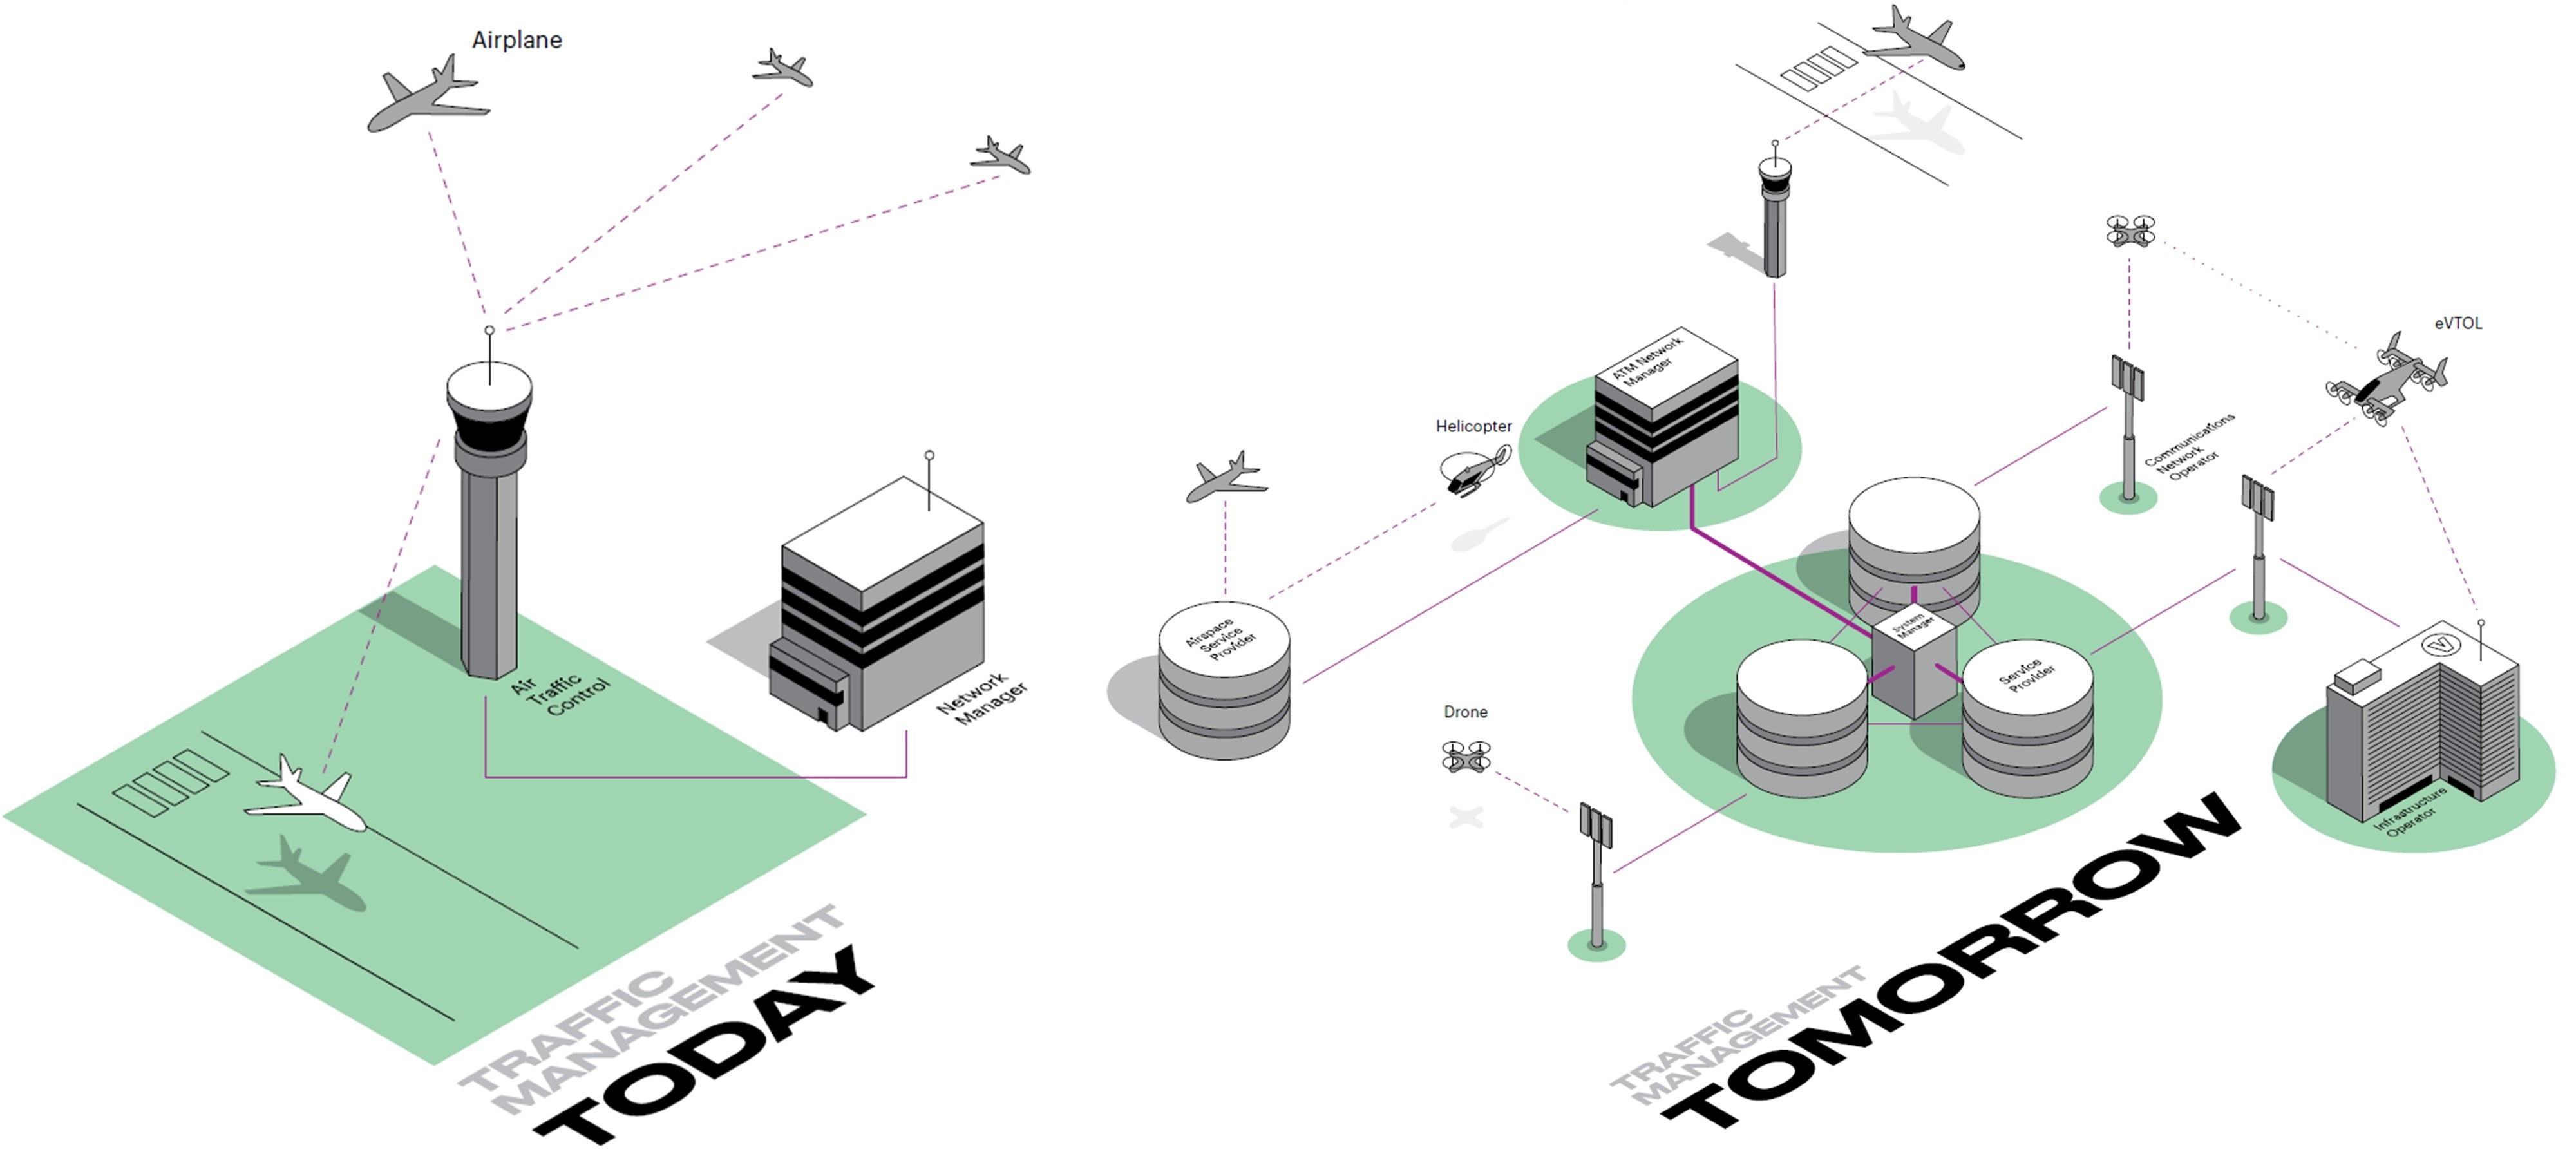
\includegraphics[width=0.9\textwidth]{\FIGDIR/I001TrafficManagement}
    \caption{Present and future \emph{Air Traffic Management} (ATC) \cite{airbusUTM2018blueprint}.}
    \label{fig:airTrafficManagementEvolution}
\end{figure}

\paragraph{UAS integraiton into Air Traffic:} The major effort is focused on \emph{Air Traffic Control} (ATC) changes. The \emph{actual} organization (sec. \ref{sec:AirspaceClassification}) and management (sec. \ref{sec:WellClear}) of airspace is centralized and \emph{human operated}.  

The \emph{ongoing changes} are shown in (fig. \ref{fig:airTrafficManagementEvolution}). The \emph{UAS Traffic Management} (UTM) (sec. \ref{sec:UTM}) complementing ATC is introduced to manage unmanned aviation. The additional traffic hubs, for UAS \emph{delivery \& transportation} services are added. The greatest change is on previously \emph{low-altitude uncontrolled} airspace, this space has new authority (UTM). The future UAS must implement mechanisms for \emph{event-based} navigation and avoidance (sec. \ref{sec:EventBasedAvoidance}).

Since 2014, there is a visible strong political support for developing rules on drones but regulations are harmonizing slowly. The European Aviation Safety Agency (EASA) has been tasked to develop a regulatory framework for drone operations and proposals for the regulation of "low-risk" UAV operations. In achieving this, EASA is working closely with the Joint Authorities for Regulation of Unmanned Systes (JARUS) \cite{jarus2016regulations}.

The \emph{operational rules} (sec. \ref{sec:AircraftOperationRules}) with \emph{rules of the air} \cite{icaoAnnex2} which are enforced now are simple. The \emph{future flight rules} (fig. \ref{fig:flightRulesIntro}) will be more complicated including the precise waypoint system and more complex missions. The future flight rules will be micro-managed by UTM. The example of such micro-management is shown in (sec. \ref{sec:UASTrafficManagement}, \ref{s:RuleEngineArchitecture}). 

The \emph{increase} of \emph{traffic density} increases the \emph{accident probability/severity}.  There are different threats endangering UAS, the \emph{obstacles} imposes eminent destruction threat, intruders can cooperate in mutual avoidance, the weather avoidance becomes more critical, the international/national authority can impose additional operational constraints. These threats needs to be well managed and prioritized to guarantee safe UAS operations.

\begin{figure}[H]
    \centering
    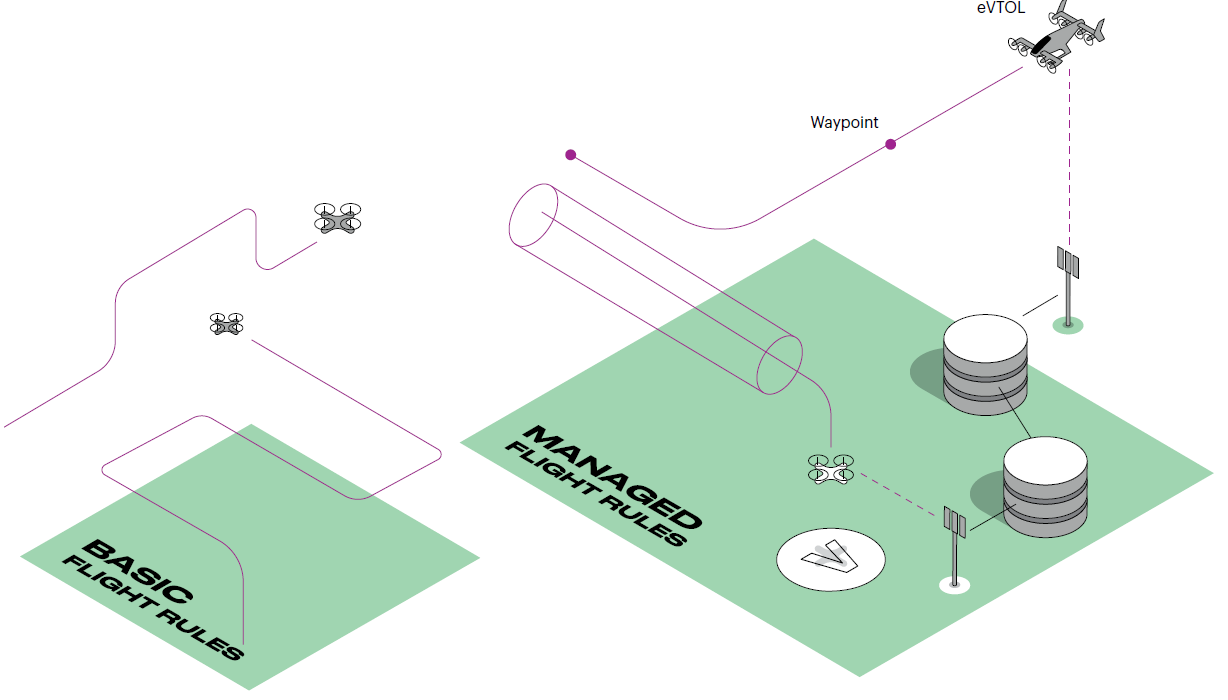
\includegraphics[width=0.8\textwidth]{\FIGDIR/I002FlightRules}
    \caption{Flight rules overview. \cite{airbusUTM2018blueprint}.}
    \label{fig:flightRulesIntro}
\end{figure}

\paragraph{Detect \& Avoid:} The other approach is bottom-up, that means the development of basic adaptable functionality to cover complex navigation/avoidance tasks in \emph{controlled airspace}. The intuitive definition of \emph{Detect \& Avoid} (DAA) functionality is given in (fig. \ref{fig:detectAdnAvoidIntroduction}).

\begin{figure}[H]
    \centering
    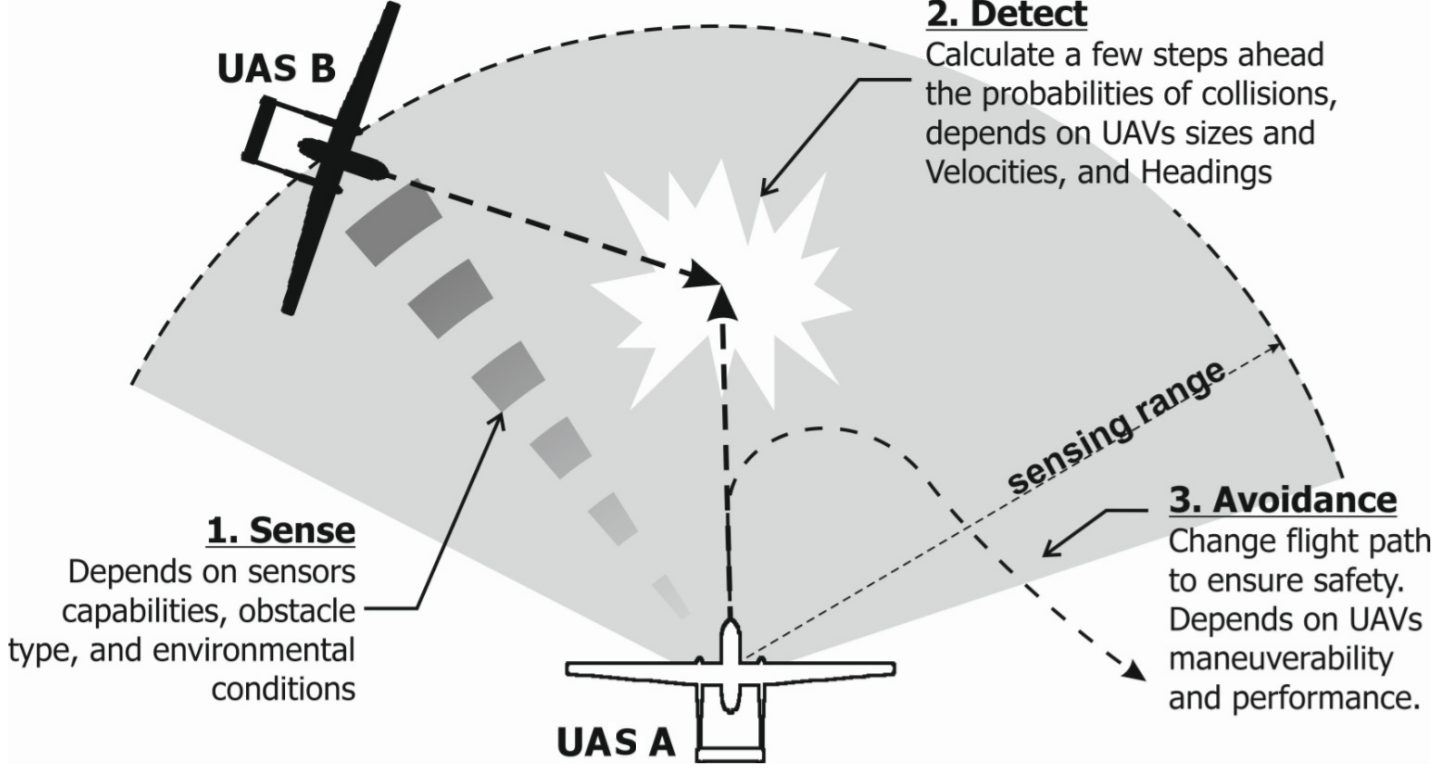
\includegraphics[width=0.6\textwidth]{\FIGDIR/I003DetectAndAvoid}
    \caption{\emph{Detect \& Avoid} (DAA) principle \cite{jenie2014velocity}.}
    \label{fig:detectAdnAvoidIntroduction}
\end{figure}

\noindent The DAA can be applied in short term (avoidance) and long term (navigation) tasks. It consist from three continuously repeating major steps:
\begin{enumerate}
    \item \emph{Sense} - the processing of intermediate sensor reading, the physical world approximation creation.
    
    \item \emph{Detect} - an addition of information from other sources to create complex situation assessment scenario, future possibilities projection and control strategy selection.
    
    \item \emph{Avoid} - execution of selected control strategy while checking possible changing events.
\end{enumerate}

The \emph{short term avoidance} (sec. \ref{s:aviudabceGridRun}) can be chained into \emph{long term navigation} (sec. \ref{s:missionControlRun}). This long term navigation can be used to solve \emph{UTM/ATM} imposed constraints, under assumption that there is sufficient \emph{data fusion} (sec. \ref{s:sensorFusion}).

\paragraph{Challenge Motivation:} Both \emph{Air Traffic Control} and \emph{Detect \& Avoid} requires a tool to assess possible UAS maneuvering:

\begin{enumerate}
    \item \emph{Air Traffic Control} needs to know the UAS maneuvering capabilities in order to \emph{validate} feasibility of \emph{issued orders} and to predict future \emph{trajectory} for \emph{collision prevention}.
    
    \item \emph{Detect \& Avoid} needs to calculate feasible \emph{system constraints feasible maneuvering strategy} in finite time to ensure own safety. 
\end{enumerate}

\paragraph{Reach Sets:} These challenges are addressable by employment of \emph{reach sets} (sec. \ref{s:ReachSets}). The \emph{reach set} is self-validating set of possible maneuvering strategies for some initial UAS state and some time-period. 

To guarantee finite time evaluation, the discretization of \emph{operation space} (sec. \ref{s:AvoidanceGrid}) and \emph{movement discretization} (sec. \ref{sec:MovementAutomatonBackground}) needs to be introduced. The discretization gives finite countable sets of choices, therefore it also guarantees finite time evaluation process.

Our \emph{implementation} of \emph{reach set approximation} (sec. \ref{s:reachSet}) enables to encode some sought behavioral patterns as natural properties (sec. \ref{s:constrainedTrajectoryExpansion}). This enables to generate specific task oriented \emph{reach set approximation} for navigation (sec. \ref{s:chaoticReachSet}), avoidance (sec. \ref{s:harmonicReachSet}), UTM behavior predictions (sec. \ref{sec:collisionCase}). 


    \section{Goals}\label{s:goals}
\paragraph{Situation:} The \emph{UAS} equipped with cooperative/non-cooperative surveillance sensors, with prior knowledge of operation space has to fly a mission represented ordered set of waypoints. The set of sensors can change depending on UAS construction. The minimal airworthiness for a given operation is assumed.

\paragraph{Problem:} Given environment and artifact definitions (sec. \ref{s:basicDefinitions}) with \emph{initial assumptions} (sec. \ref{s:initialAssumptions}) and \emph{incremental problem definition} (sec. \ref{s:IncrementalProblemDefinition}) develop \emph{obstacle avoidance framework} which will satisfy \emph{avoidance} (sec. \ref{s:AvoidanceRequirements}) and \emph{navigation} (sec. \ref{s:navigationRequirements}).

\paragraph{Expected Solution:} Define an approach based on \emph{reach sets} which are capable of:

\begin{enumerate}
    \item \emph{Static obstacle avoidance} - to avoid the ground, man-made structures in open terrain. 
    
    \item \emph{Intruders avoidance} - to avoid flying objects which does not have the intention to harm our UAS, detected in sufficient distance. 

    \item \emph{Geo-fencing support} - to avoid known zones/airspace portions, which have forbidden entry.

    \item \emph{Weather avoidance} - to avoid known zones of harmful weather conditions.

    \item \emph{Cooperative conflict resolution} - to communicate own position to authority and to follow authority orders.
    
    \item \emph{Treat prioritization} - to assess avoidance according to natural or man-made priorities. (Rather break geo-fence, than crashing into the ground).
\end{enumerate}

\paragraph{Validation:} Develop test-framework to showcase approach properties. Define \emph{test scenarios} (sec. \ref{s:testingApproach}) to validate \emph{Expected Solution Performance} (sec.  tab. \ref{tab:testCasesSummary}) concerning \emph{avoidance capability} (sec. \ref{s:performanceEvaluationTable}) and \emph{computational feasibility} (sec. \ref{s:ComputaitonFootprint}).

\paragraph{Application Requirements:} There are  following application requirements, based on similar applications for \emph{manned aviation} and \emph{industry expectations}:

\begin{enumerate}
    \item \emph{Low-performance requirements} - the computational footprint of the approach should be polynomial. The most of actual UAS systems have \emph{embedded computer} with low computation power.
    
    \item \emph{Deterministic} - the \emph{avoidance strategy} should be achieved in finite time frame. The mandatory requirement for \emph{airborne operation support application}, the advice needs to be reproducible under the same conditions.
    
    \item \emph{Scalability} - the \emph{avoidance framework} should be portable to the different platforms, and it should work with different sensor array. The interface requirement for \emph{control} and \emph{data fusion} coming from other \emph{collision avoidance systems}.
    
    \item \emph{Adaptability} - the \emph{avoidance process} should have tuning points where is possible to change behavior according to UAS context. The regulations are changing with location, time and circumstances, the part of calculation/control process needs to be implemented dynamically.
\end{enumerate}
    \section{ Overview}\label{s:Overview}

\noindent The thesis is organized like follows:

\begin{enumerate}
    \item \emph{Introduction} (ch. \ref{ch:introduction}) - the introduction chapter giving an overview of work motivation, goals, contributions and \emph{author`s list of publication}.
    
    \item \emph{Collision Avoidance} (ch. \ref{ch:CollisionAvoidance}) - This chapter gives aerospace-related background. The manned aviation is serving as the knowledge base for an assumption of future UAS Detect \& Avoid functionality. The chapter gives overview of airspace classification, which told us where and what we can do or expect. Aircraft operational rules for general are reflected into \emph{separation functionality}. The separation can be passively enforced by Air Traffic Management authority or active enforced by \emph{ACAS-X/TCAS} systems. The \emph{UAS Traffic Management} is parallel to manned aviation practices with additional layer of complexity.  The \emph{Event-Based avoidance} is introduced to give overview of concepts used later.
    
    \item \emph{Background Theory} (ch. \ref{ch:backGroundTheory}) - this chapter outlines background necessary for approach understanding. The \emph{control theory} system models are used as a base for the \emph{reach set} calculation. The important concept of \emph{hybrid automaton} (special case of hybrid automaton) is introduced. The LiDAR related theory and complements are presented at last. 
    
    \item \emph{Problem Statement} (ch. \ref{c:problemStatement}) - this chapter states the problem solved in this work. The basic definition and terminology are established at beginning with initial problem and assumptions. Incremental problem is introduced with increasing complexity and relaxed conditions. Avoidance and Navigation functional and non-functional requirements are stated at last. 
    
    \item \emph{State of Art} (ch. \ref{ch:stateOfArt}) - this chapter covers important results of other researcher works in topics of Movement Automaton, Sensor \& Data Fusion, Navigation Algorithm, Reach Sets, and Testing Approach. The \emph{UAS Traffic Management} concept relevant to this work is introduced.  
    
    \item \emph{Approach} (ch. \ref{ch:approach}) - this chapter describes the approach, it starts with an overview (sec. \ref{s:approachOverview}), outlining the block scheme of the system (fig. \ref{fig:AvoidanceFrameworkConceptNew}). The discretization of the space, trajectories, and system model are covered in (sec. \ref{s:modelMAImplementation} - \ref{s:AvoidanceGrid}), the following topics are covered:
    \begin{enumerate}[a.]
        \item \emph{Reach Set Estimation} (sec. \ref{s:reachSet}) - the discretization, performance evaluation, and generation algorithms.
        
        \item \emph{Encounter Modeling} (sec. \ref{s:staticObstacles} - \ref{s:intruders}) - static obstacles, intruders, static/moving constraints, and more.
        
        \item \emph{Collision Avoidance} (sec. \ref{s:avoidanceConcept}) - the avoidance/navigation loop with global data fusion procedure, complexity and safety margin calculations.
        
        \item \emph{Further to Cooperative Operations} (sec. \ref{sec:UASTrafficManagement} - \ref{sec:ruleEngine}) - the approach to satisfy scalability and \emph{UTM} requirements.
    \end{enumerate}
    
    \item \emph{Simulations} (ch. \ref{Simulations}) the simulations cover aspects developed in approach, the test plan (tab. \ref{tab:testCasesSummary}) summarizes test cases. The results are outlined in (tab. \ref{tab:testCasesPerformacneEvaluation}), the computation load statistics are summarized in (tab. \ref{tab:computationLoadStatistics}). The tests are divided into the following categories:
    
    \begin{enumerate}[a.]
        \item \emph{Non-cooperative Test Cases} (sec. \ref{s:noncooperativeTestCases}) - various obstacles, weather constraints, and non-cooperative intruders test cases
    
        \item \emph{Cooperative Test Cases} (sec. \ref{s:cooperativeTestCases}) - maneuvers in controlled airspace under supervision of traffic management.
    
        \item \emph{Reach Set Estimation Performance and Properties} (sec. \ref{sec:reducedReachSetPerformance}) - the comparison of various estimation methods, the impact on complexity.
    \end{enumerate}
    
    \item \emph{Conclusion and Future Work} (ch. \ref{ch:Conclusion}) - work conclusion, summarizing achieved results, comparing other approaches, outlining reusable modular parts of approach, utilizing the future work on approach shortcomings.
\end{enumerate}
    \section{(R) Contributions}\label{s:Contributions} 
\noindent The \emph{contributions} of this work can be divined into two categories:
    
\paragraph{Conceptual Contributions:} The contributions enhancing and enriching the conceptual level of \emph{Detect \& Avoid} systems, namely:

\begin{enumerate}
    \item \emph{Movement automaton control and prediction} -  necessity to abstract the control of the system from the \emph{detect and avoid} systems, leads to customization of hybrid automaton (sec. \ref{s:HybridAutomaton}) to \emph{movement automaton} (def. \ref{s:MovementAutomatonDefinitionAndProperties}). The movement automaton can be adapted to nonlinear system (sec. \ref{s:UASNonlinearModel}) as a instance (sec. \ref{s:movementAutomatonDefinition}). The movement automaton can be also used as a predictor of the system (sec. \ref{s:referenceTrajectoryGenerator}). The \emph{initial state disparity issue} \cite{gomola2017obstacle} has been addressed in (sec. \ref{s:segmentedMovementAutomaton}).
    
    \item \emph{Trajectory as a discrete command chain} -  the \emph{movement automaton} as a control interface consuming the discrete command chain enabled the \emph{finite discrete representation} of trajectory (eq. \ref{eq:ourTrajectoryImplementation}).
    
    \item \emph{Reach set discretization} - the \emph{infinite reach set} (def. \ref{}) can be represented as a tree of movements from system initial state (def. \ref{def:ReachSetApproximationByMovementAutomaton}). This tree can have associated properties, like reachibility of each trajectory segment (eq. \ref{eq:trajectoryReachibility}).  The advantage of having finite maneuver set, with little precision sacrifice, which can be calculated prior the flight have huge impact on \emph{computation complexity} (sec. \ref{sec:MCRcomputationalComplexity}). Enabling to use approach on different platforms with small computational power. 
    
    \item \emph{Operational space assessment} - the operational space is separated by grid into finite set of the cells. Each cell has properties to track like the occurrence of obstacle, presence of intruder or impact of constraint. The \emph universal data fusion procedure (sec. \ref{s:sensorFusion}) is enabling accumulation of treat information from various sources.
    
    \item \emph{Hierarchical threat assessment} -  the \emph{various threat} sources (obstacles, intruders, constraints) are categorized according to operational environment/rules and their avoidance priority is handled according to that (fig. \ref{fig:missionControlRunActivityDiagram}).
    
    \item \emph{UAS Traffic Management} - the architecture proposal for traffic management  as cooperative authority (sec. \ref{sec:utmArchitecture}) covers some basic maneuvers (sec. \ref{sec:handlingHeadOnApproach}, \ref{sec:handlingConvergingManuever},\ref{sec:handlingOvertakeManuever}), the more important is the adaptability of presented approach to cooperative (sec. \ref{sec:cooperativeConflictResolution}) and non-cooperative (sec. \ref{sec:nonCooperativeConflictResolution}) avoidance modes, showing adaptability. 
\end{enumerate}

\paragraph{Implementation Contributions:} The concepts, which solve implementation issues for \emph{Detect \& Avoid} systems, namely:

\begin{enumerate}
    \item \emph{Operational space segmentation} - the \emph{planar grid} (sec. \ref{s:AvoidanceGrid}) slice (fig. \ref{fig:LidarSpaceSegmentation}) have been selected, because it can be used for fast assessment of LiDAR scan data to estimate, obstacle (\ref{fig:P01CountOfLiDARHits}) or visibility (\ref{fig:P02OvershadowedMapobstacle}). The cell volume is increasing with distance from UAS, this gives us decreased space status assessment complexity.
    
    \item \emph{Wave-front algorithm for avoidance estimation} - to estimate reach set the space exploration method has been developed. The \emph{rapid exploration tree} (fig. \ref{fig:rapidExplorationTrajectoryTree}) is employed as \emph{wave-front} expansion (alg. \ref{alg:Wavefront Propagation}). Various shapes and properties of \emph{reach set estimation} can be achieved employing the \emph{constrained expansion functions} for \emph{chaotic} (alg. \ref{alg:ExpansionConstraintFunctionForChaoticReachSet}), harmonic (alg. \ref{alg:ExpansionConstraintFunctionForHarmonicReachSet}), and, \emph{ACAS-like} (alg. \ref{alg:ExpansionConstraintFunctionForACASLikeReachSet}) reach set approximations.
    
    \item \emph{Encounter and constraints models} - the planar grid used in solution required a development of encounter models for static obstacles, constraints (sec. \ref{s:staticObstacles}), intruders, moving constraints (sec. \ref{s:intruders}). The intersection algorithms can be reused in other approaches using unusual grid.
    
    \item \emph{Avoidance process enhancement (Rule engine)} - the air traffic rules are changing based on time and geographic location, the UTM concept is under development. These reasons are calling to use flexible implementation architecture, rule engine (sec. \ref{s:RuleEngineArchitecture}). The rule engine can be set to cover any kind of rules (fig. \ref{fig:RuleEngineInstanceLevels}).
\end{enumerate}
    \section{\secState{R}List of Publications}\label{sec:listOfPublications}

\noindent This \emph{section} contains the list of published articles, proceedings, technical reports and module projects, relevant to the \emph{thesis topic}.

%   My First Article Ever!
\paragraph{Article:} Alojz Gomola, Joao Borges de Sousa, Fernando Lobo Pereira, and Pavel Klang. Obstacle avoidance framework based on reach sets. In Iberian Robotics conference, pages 768–779. Springer, 2017. \cite{gomola2017obstacle}\footnote{Draft available online: \url{https://goo.gl/kZujZE}}.

\emph{Summary:} This report on preliminary investigations concerning the development of a LiDAR-based detect and avoid (DAA) system with a low computational footprint for small Unmanned Air Systems. The focus is on the integration with nominal flight control systems and computational feasibility. The proposed system decomposes the SAA problem into the following components detection, space assessment, escape trajectory estimation and avoidance execution. The control logic is encoded with the help of a hybrid automaton. The properties of the system are studied with the help of approximations to time slices of the UAV reach set.


\paragraph{Article:}  Juraj {\v{S}}tevek,  Michal  Kvasnica,  Miroslav  Fikar,  and  Alojz  Gomola. A  parametric programming  approach  to  automated  integrated  circuit  design. IEEE Transactions on Control Systems Technology, 26(4):1180–1191, 2018. \cite{vstevek2018parametric}\footnote{IEEE copy online: \url{https://ieeexplore.ieee.org/stamp/stamp.jsp?arnumber=7981386}}.

\emph{Summary:} The proposal of an optimization-based slotting approach to automated \emph{integrated circuit} design for generating a power transistor. The original slotting problem is formulated as a mixed-integer linear program. It is solved through parametric optimization with an advantage that usage of any commercial optimization solvers on user’s side is avoided with short evaluation time and simple implementation. The approach is applied in specific very large scale integration production technology and demonstrated on an example.

\emph{Contributions:} Point-location algorithm for MPC region selection. 

\paragraph{Proceedings:} Kristian Klausen, Jostein Borgen Moe, Jonathan Cornel van den Hoorn, Alojz Gomola, Thor I Fossen, and Tor Arne Johansen. Coordinated control concept for recovery of a fixed-wing uav on a ship using a net carried by multirotor UAVs.  In Unmanned Aircraft Systems (ICUAS), 2016 International Conference on, pages 964–973. IEEE, 2016, \cite{klausen2016coordinated}\footnote{Public copy available online: \url{http://folk.ntnu.no/torarnj/ICUAS2016_singlecolumn.pdf}}.

\emph{Summary:} Ship-based Unmanned Aerial Vehicle (UAV) operations represent an important field of research which enables a large variety of mission types. Most of these operations demand a high level of endurance which normally requires the use of a fixed-wing UAV. Traditionally, a net located on the ship deck is used for recovering the fixed-wing UAV. However, there are numerous challenges when attempting autonomous landings in such environments. Waves will induce heave motion, and turbulence near the ship will make approaches challenging. In this paper, we present a concept using multi-rotor UAVs to move the recovery operation off the ship deck. To recover the fixed-wing UAV, a net is suspended below two coordinated multirotor UAVs which can synchronize the movement with the fixed-wing UAV. The approach trajectory can be optimized with respect to the wind direction, and turbulence caused by the ship can be avoided. In addition, the multirotor UAVs can transport the net at a certain speed along the trajectory of the fixed-wing UAV, thus decreasing the relative velocity between the net and fixed-wing UAV to reduce the forces of impact. This paper proves the proposed concept through a simulation study and a preliminary control system architecture.

\emph{Contributions:} Ground station maneuver implementation, messaging between ground station/UAVs. RTK-GPS for precise navigation integration, Net-release mechanism design, Mechanical parts for 3D printer modeling. 

\paragraph{Proceedings:}  Alojz Gomola.  An aspect-oriented solution for mutual exclusion in embedded systems. In Alena Kozakova, editor, ELITECH15: 17th Conference of doctoral students, pages 964–973, Bratislava, Slovak Republic, May 2015. Online publication, \cite{gomola2015aspectOriented}\footnote{Draft available online: \url{https://github.com/logomo/Elitech15-paper}}.

\emph{Summary:} Embedded systems are developed for a wide range of applications. The best-known applications are industrial process control and banking solutions. Fault tolerance is a crucial requirement in long-term embedded systems. This paper presents solution for mutual exclusion in embedded systems. The usual mutual exclusion solution using semaphores is a crosscutting concern. Semaphores are difficult to maintain in code, and their failure rate is high. We propose new aspect-oriented solution for mutual exclusion. Our solution utilizes aspect-oriented approach, is usable in other systems and designed to be robust against program changes, and it provides a solution to aspect fragility problem.

\paragraph{Technical report:} Alojz Gomola, Pavel Klang, and Jan Ludvik. Probabilistic approach in data fusion for obstacle avoidance framework based on reach sets. In Internal publication collection, pages 1–93. Honeywell, 2017, \cite{gomola2017probabilistic}\footnote{Public copy available online: \url{https://github.com/logomo/Data-Fusion-Report}}.

\emph{Summary:} The \emph{sensor input} and \emph{information sources} fusion procedure design to obtain rated space assessment for visibility, obstacle occupancy, and reachability evaluation. A unique statistical approach was proposed to couple partial ratings under reading and time uncertainty. The key contribution is scalable approach to evaluate \emph{UAS action space} and \emph{Feasible Trajectories} properties. 

\paragraph{Technical report:}  Alojz Gomola. Model predictive control of unmanned air vehicles with obstacle avoidance capabilities, technical report, FEUP, 2017, \cite{gomola2017mpc}\footnote{Public copy available online: \url{https://github.com/logomo/Predictive-control---Final-report}}.

\emph{Summary:} Initial solution of \emph{predictive control} problem for \emph{UAS} navigation in constrained, non-controlled airspace. The key contribution is \emph{Movement Automaton} (a special type of hybrid automaton) establishment in current form (sec. \ref{sec:MovementAutomatonBackground}). The \emph{stability}, \emph{controllability} and \emph{observability} properties have been proven. The \emph{feasibility} of \emph{Movement Automaton} as \emph{control interface} and \emph{future state predictor} has been shown through formal proof and excessive testing.

\paragraph{Technical report:} Alojz  Gomola.   Optimal  control  of  unmanned  air  vehicles  with  obstacle  avoidance capabilities in partially known environment.  Technical report, FEUP, 2017. \cite{gomola2017optimal}\footnote{Public copy available online: \url{https://github.com/logomo/Optimal-Control}}.

\emph{Summary:} The \emph{optimization problem} for \emph{obstacle avoidance} (eq. \ref{eq:trajectoryTrackingOptimalizaitonProblem}) to satisfy \emph{avoidance requirements} (sec. \ref{s:AvoidanceRequirements}) 

\paragraph{Framework:} Feature-based ACAS\footnote{Matlab prototype available online: \url{https://github.com/logomo/Feature-based-ACAS}} implementation to support claims of this work has been developed through the course of years \emph{2016-2019}. The framework provides: 
\begin{enumerate}
    \item \emph{Simulation environment} - full support for single/multiple UAS simulation support in controlled/non-controlled airspace.
    
    \item \emph{Mission Control Support} - standard mission control support for \emph{sparse ordered waypoint} mission type. 
    
    \item \emph{UAS Traffic Management} - support for \emph{collaborative} weather and collision avoidance with general authority in controlled airspace. The configurable \emph{event-handling} through \emph{rule-engine}.
    
    \item \emph{Encounter Models} - the model for \emph{static obstacles} supporting point-cloud generation of LiDAR sensor, various intruders model supporting the ADS-B like encounter model, static/dynamic polygon constraints with altitude range. 
    
    \item \emph{Collision Avoidance} - the support for \emph{cooperative} and \emph{non-cooperative} behavior in controlled airspace, \emph{non-collaborative, non-adversary} behavior in non-controlled airspace. 
    
    \item \emph{Reach Set Estimation Methods} - four methods for various property focused \emph{Reach Set Estimations}.
\end{enumerate}

%02-Collision Avoidance
    \cleardoublepage
\chapter{Collision Avoidance}\label{ch:CollisionAvoidance}
\noindent The context of Collision Avoidance is introduced in (tab. \ref{tab:CASContext}), the structure was taken from Gardi \cite{gardi2015automated}. The \emph{state of art} changes was incorporated into the table.

\begin{tabularx}{\textwidth}{S{0.20}||S{0.55}} 
    \centering \emph{Function} &  \emph{Equipment/Task}\\ \hline\hline
    \centering Communication & Telecommunication datalinks,\newline Controller Pilot Data Link-Control (CPDLC), \newline Voice Communication\\\hline
    \centering Navigation & Navigation sensors including GNSS, INS, etc. providing 3D/4D navigation capabilities.\\\hline
    \centering Surveillance & Cooperative Systems (TCAS, ACAS, etc.)\newline Non-cooperative Sensors (LiDAR,Cameras, etc.)\\\hline
    \centering Situation\newline Awareness& Early Warning Systems, \newline CDTI Display\\\hline
    \centering{Autonomous\newline{Decision}\newline{Making}}& Strategic, Tactical, Emergency Flight Planning,\newline Intelligent Collision Detection,\newline Conflict Resolution and Prevention,\newline Weather/Terrain/Constraints Avoidance\\
    \caption{Collision avoidance systems context overview \cite{gardi2015automated}.}
    \label{tab:CASContext}
\end{tabularx}

\newpage
\section{Overview}\label{s:collisionAvoidanceOverview}
\noindent The \emph{Detect and Avoid}, as a part of \emph{Collision Avoidance}, impacts all collision avoidance aspects (tab. \ref{tab:CASContext}). This work focuses on the \emph{Reach Sets} which gives us the following focus area:

\begin{enumerate}
    \item \emph{Communication} - it is assumed the command \& control communication link is stable. This aspect is not affected by reach sets.
    
    \item \emph{Navigation} - minimal navigation framework needs to be implemented for full experimentation with the navigation capabilities of the \emph{Reach Set} based trajectory generation.
    
    \item \emph{Surveillance} - the surveillance will be covered with necessary low-cost technologies, the simulated sensor inputs for following surveillance equipment is considered:
    \begin{enumerate}[a.]
        \item \emph{Non-cooperative} - LiDAR Sensor.
        \item \emph{Cooperative} - ADS-B In/Out.
    \end{enumerate}
    
    \item \emph{Situation  awareness} - the situation awareness focuses on \emph{space segmentation} and \emph{safety evaluation} to support proper safe trajectory selection from \emph{reach set}.
    
    \item \emph{Autonomous decision making} - the \emph{reach set} covers all possible avoidance strategies, to know how to select proper strategy is key in successfully avoidance maneuvering.
\end{enumerate}

\paragraph{Communication:} An overview elaboration on capability, reliability, security, architecture have been summarized  by Johansen et al. in \cite{johansenetal2018surveyCommunicaiton}.

The current state of art \emph{communication lines} and relay approaches are sufficient to provide necessary utilities. The use of an existing 4G/3G mobile network is the most probable candidate for low altitude UAS operations. The necessity to build a back-up network for communication is still an open topic.

\paragraph{Navigation:} An overview is given by Nex \cite{nex2014uav} \emph{Waypoint planning in a 3D environment} is elaborated in \cite{bodin2007navigating}. \emph{Waypoint Tracking and Test Environments} are thoughtfully discussed in \cite{how2008real,girard2004border,andrade2017autonomous,klausen2017nonlinear}. 

All navigation methods are fairly similar. Consisting of the following steps in the loop:
\begin{enumerate}
    \item Select goal waypoint.
    \item Evaluate feasible navigation strategies (cost function).
    
    \item Select navigation strategy and generate reference trajectory.
    
    \item Follow the reference trajectory with UAS system.
\end{enumerate}
The \emph{evaluation process} and selection criteria need to be designed in the context of \emph{reach sets}.

\paragraph{Surveillance:} TCAS and ACAS systems cover the cooperative surveillance, an interesting aspect of these systems are \emph{Resolution Advisories} \cite{kennedy1995resolution} for TCAS \cite{marston2015acas}, for ACAS.  These advisories are giving the suggestions for the pilot to avoid an occurring collision. The responsibility for following advisories and avoiding collision is on the pilot.  

This mechanism needs to be changed to increase the determinism of UAS behavior. The voluntary approach of advisories needs to be replaced with a mandatory approach (directives).

\paragraph{Situation awareness:} The aspect of the situation awareness of surroundings has been introduced in \cite{blaskovich2007declutter}. \emph{LiDAR}-based \emph{SAA} system has been introduced by Sabatini \cite{sabatini2014lidar} further enhanced by Ramasay \cite{ramasamy2016lidar}. Other \emph{Non-Cooperative} sensors and their feasibility have been outlined in Ramasay work \cite{ramasamy2014avionics}. 

The common ground of these works is an operational space discretization into various forms of finite discrete sets to enable deterministic decision making. The key issue is to find a good rate between space democratization and solution precision. The large cells in the grid usually hide many escape routes. The small cells in grid usually increase the computational complexity and diminish computation time optimal solution.

Examples of \emph{situation awareness:} implementation can be found mainly in \emph{human-centered} systems, \emph{Early Warning System} has been proposed by Lee \cite{lee2002collision} and an adaptive version by Miller \cite{miller2002adaptive}. Effects of \emph{CDTI Display} visualization and human decision impact have been examined by Thomas \cite{thomas2005effects}. \emph{Self Separation} aspect has been examined by Williams \cite{williams1983self}.

\noindent
The important concept for \emph{UAS} is internal data representation and autonomous situation resolution. The autonomous situation resolution (decision-making process) can be extracted from human pilot operation procedures.  

\paragraph{Manned Aviation Concepts:} The introduction of necessary concepts from manned aviation is organic in UAS concept understanding. 
Many of the concepts are taken directly from manned aviation. The main contribution is to change the \emph{human decisions} into \emph{autonomous system decisions}.

\paragraph{Airspace Classification:} For integration of the UAS systems into non -segregated airspace it is necessary to know the classification of the \emph{operational space}. Who is the authority, in which space, and when the authority is enforced. The general overview of airspace classes and concepts accepted by ICAO/FAA/EASA are outlined in (sec. \ref{sec:AirspaceClassification}). The common viewpoint is emphasized. 
    
\paragraph{Aircraft Operational Rules:} It is necessary to know the basic rules in controlled/uncontrolled airspace. What is expected to be done by the aircraft in various flight modes. What is minimal equipment's, what is airworthiness and so on. The basic regulations are outlined in (sec. \ref{sec:AircraftOperationRules}). Visual Flight Rules (VFR) interesting parts can be found in (sec. \ref{sec:VisualFlightRules}). Instrumental Flight Rules interesting parts can be found in (sec. \ref{sec:InstrumentalFlightRules}).
        
\paragraph{Active/Passive Separation and Self-Separation:} The \emph{safe navigation} in \emph{airspace} have multiple levels, going from least strict to very strict and keeping aircraft or UAS \emph{well clear} of all threats. There is first protective barrel known as \emph{well clear}; then there is a smaller protective barrel representing \emph{near miss}, then the smallest protective barrel representing \emph{crash zone}. The \emph{Well clear} state of aircraft/UAS in airspace  important parts are mentioned in (sec.\ref{sec:WellClear}). 

The important role of \emph{Air Traffic Control} for manned aircraft is introduced in  (sec. \ref{sec:AirTrafficControl}). The general aviation \emph{routing} principles can be used on the various scale for \emph{UAS routing}. The form of \emph{ATC} commands and directives must persist in future UAS traffic management, for compatibility reasons.

The current Collision Avoidance Systems systems TCAS (\ref{sec:TCAS}) and ACAS-X (\ref{sec:ACASX}) which can be used as unmanned approach base are introduced.

\paragraph{UAS Traffic Management:} The traffic management functionality is analyzed in (sec. \ref{sec:UTM}), two major movements EU USPACE (\ref{sec:USpace}) and US NASA UTM (\ref{sec:NASAUtm}) exists. The most notable information from operation specification is extracted there.

\emph{Event-Based Avoidance} (sec. \ref{sec:EventBasedAvoidance}) defines basic event-based control invoked by \emph{UTM}; two major categories are analyzed in \emph{Mid-Air Collision Prevention} (sec. \ref{sec:MidairCollisionPrevention}) and \emph{Weather Impact} (sec. \ref{sec:WeatherImpact}).
    \section{(W) Airspace classification}\label{sec:AirspaceClassification}
\begin{itemize}
    \item Airspace classes,
    \item Controlled airspace (Risk analysis, Actors)
    \item Uncontrolled airspace (Risk analysis, Actors)
    \item Aircraft categorization
    \item MOPS for different airspace 
\end{itemize}
    \section{(R) Aircraft Operational Rules}\label{sec:AircraftOperationRules}
\paragraph{Motivation:} The \emph{aircraft operation rules} are ranging from personal, trough technical, to standardization category. In this section the \emph{flight rules} will be outlined in necessary depth for \emph{collision avoidance}. the goal of this section is to give an overview of airspace constraints. 

\paragraph{Rules Origin:} The \emph{Rules of the Air} are provided by following documents:

\begin{enumerate}
    \item \emph{SERA Regulation 923/2012} - laying down the common rules of the air and operational provisions regarding services and procedures in air navigation and amending Implementing Regulation (EU) No 1035/2011 and Regulations (EC) No 1265/2007, (EC) No 1794/2006, (EC) No 730/2006, (EC) No 1033/2006 and (EU) No 255/2010 \cite{rulesOfTheFlight2012} notable contributions:
    \begin{enumerate}[a.]
        \item \emph{Table of cruising levels} - Appendix III.
        \item \emph{ATS airspace classes — services provided and flight requirements} - Appendix IV.
    \end{enumerate}
    
    \item \emph{SERA Regulation 2016/1185} - Commission Implementing Regulation (EU) 2016/1185 of 20 July 2016 amending Implementing Regulation (EU) No 923/2012 as regards the update and completion of the common rules of the air and operational provisions regarding services and procedures in air navigation (SERA Part C) and repealing Regulation (EC) No 730/2006.

    \item \emph{ICAO  Annex II.} - the \emph{mostly accepted} rules of the air document \cite{icaoAnnex2}, providing general rules of the air (sec. \ref{sec:handlingHeadOnApproach}, \ref{sec:handlingConvergingManuever}, \ref{sec:handlingOvertakeManuever}).
\end{enumerate}

\begin{note}
    This section contains important parts from previously mentioned documents. 
\end{note}

\subsection{(W) Visual Flight Rules (VFR)}\label{sec:VisualFlightRules}
\begin{itemize}
    \item Rules of the Air
    \item Visual separation
\end{itemize}

\subsection{(W) Instrumental Flight Rules (IFR)}\label{sec:InstrumentalFlightRules}
\begin{itemize}
    \item Instrumental separation
    \item Alert/Notice definition
    \item Prioritization IFR/VFR
\end{itemize}

	%02-04 Remaining well clear
    \section{\secState{R}Separation from Air Traffic}\label{sec:WellClear}

\paragraph{Remaining "Well Clear":} The separation from \emph{air traffic} is an activity when \emph{our airplane} tries to stay away from other traffic in safe manner.  

Before the definition of what is safe, there is a need for some margin definitions around the aircraft. The margins are enclosing a space in form of barrel, where \emph{airplane position} is center, the horizontal plane is base for circular boundary, the vertical axis is base for \emph{distance boundary} (fig. \ref{fig:WellClearTreshold}).

\begin{figure}[H]
    \centering
    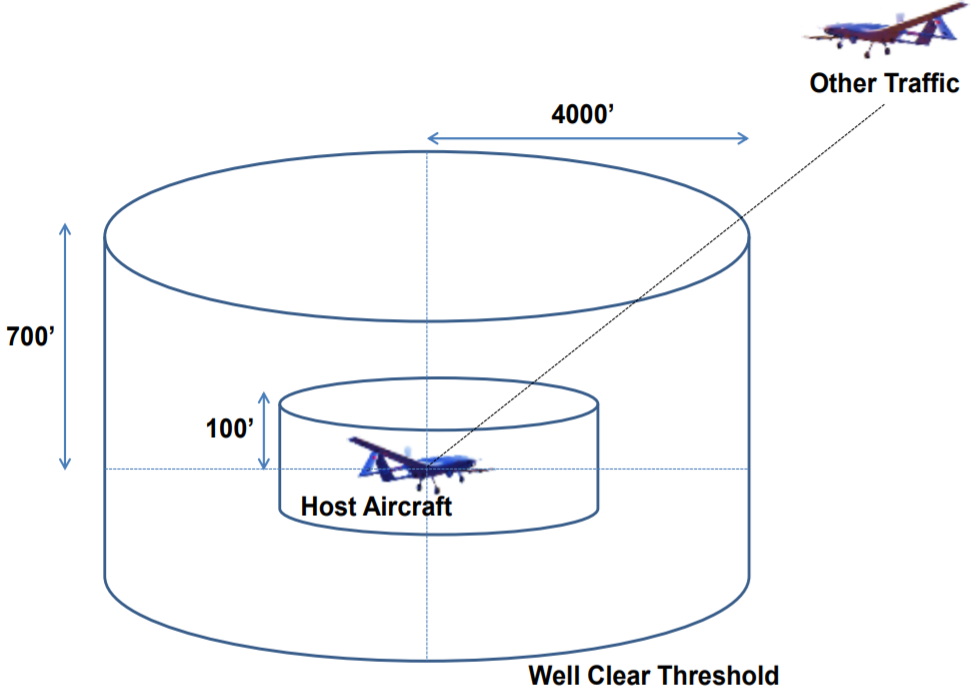
\includegraphics[width=0.6\textwidth]{\FIGDIR/02_05_WellClearTreshold}
    \caption{Well Clear Threshold \cite{valavanis2015uav,united1983pilots}.}
    \label{fig:WellClearTreshold}
\end{figure}

\noindent The boundaries and margins classification is taken from \cite{united1983pilots,valavanis2015uav} and goes like follow:

\begin{enumerate}
    \item \emph{"Alert"} - the distance to at least one surrounding aircraft is within \emph{alert margin}, the pilot is alerted about the possible threat, no action is required from pilot side.
    
    \item \emph{"Well Clear"} - the intruder enters into \emph{well clear range}, the intruder is threatening the \emph{airplane} directly, the pilot is noticed about security incident.
    
    \item \emph{"Near Miss"} - the intruder gets very close to \emph{airplane}, the body hit or \emph{turbulence impact} is very probable. 
    
    \item \emph{"Body Hit"} - the intruder stuck the \emph{airplane body}.
\end{enumerate}

\noindent These incidents are increasing their severity, the goal of separation is to keep every airspace attendant \emph{well clear}, outside well clear threshold (fig. \ref{fig:WellClearTreshold}). 
\paragraph{Air Traffic Control:} The air traffic control have passive role in separation, it manages the airspace and gives \emph{clearance} for air space users actions. There is active support for VFR (sec. \ref{sec:VisualFlightRules}) and IFR (sec. \ref{sec:InstrumentalFlightRules}). The role of \emph{Air Traffic Control} is discussed in (sec. \ref{sec:AirTrafficControl})

\paragraph{ACAS-X/TCAS:} There is support systems fo prevent \emph{Airborne Collision}, which are supporting the \emph{active avoidance} for \emph{IFR} flights (sec. \ref{sec:InstrumentalFlightRules}). Their role is to provide the surveillance of \emph{airplane} surroundings and give advisories to pilot. More about next generation system family ACAS-X can be read in (sec. \ref{sec:ACASX}). The current generation \emph{Airborne Collision} System TCAS is discussed in (sec. \ref{sec:TCAS}).


    	\subsection{(R) Air Traffic Control}\label{sec:AirTrafficControl}
\paragraph{Motivation:} The modern \emph{Air Traffic Control} (ATC) procedures are outlined in ICAO 4444 \cite{icao4444}. The ATC roles and responsibilities in terms of \emph{clearance}, \emph{self-separation}, and, \emph{provided traffic information} are summarized in (tab. \ref{tab:airspaceResponsibilitiesIcao}). 

The \emph{main role} of \emph{Air Traffic Control} (ATC) is to support the organization of the \emph{airspace} in terms of \emph{preemptive} detect and avoid.

\begin{note}
    The \emph{Reactive} and \emph{Event Based} detect and avoid for manned aviation are covered by \emph{ACAS-X/TCAS systems} (sec. \ref{sec:ACASX}, \ref{sec:TCAS})
\end{note}

\paragraph{Commands issued by ATC:} There is multiple levels of commands issued by ATC, their characteristics and compulsory level is defined as folow:

\begin{enumerate}
    \item \emph{Notification} - the information notification, commonly known as \emph{NoTice to AirMan} (NOTAM), depending on flight mode, can be transmitted as voice message or information broadcast. They usually contains information about weather and traffic situation in given sector.
    
    \item \emph{Warning} - directed message to specific general aviation  which may require some direct action. The information is usually informative, but the action is not mandatory.
    
    \item \emph{Recommendation} - directed message to specific general aviation  which requires direct action. The order is usually specific action, but the action is not mandatory to be executed by pilot.
    
    \item \emph{Directive} - directed message to specific general aviation  which requires direct action. The order is specific action and the order fulfillment is mandatory for the pilot. 
\end{enumerate}

\paragraph{Separation enforcement:} The \emph{separation} is main feature of the ATC in controlled airspace of airports (B, C, D class). Its enforced by management of \emph{action clearance}. The ATC issues the clearance for take-off/landing sequence. 

The clearance for climb/descent is given at the beginning when flight plan is approved. The ATC issues the time slots for selected pathways. The continuous monitoring of air traffic is executed in periods. The airplane deviation from cleared plan should be minimal. 

If there is any incident the the \emph{ATC} can take following actions:
\begin{enumerate}
    
    \item \emph{Heading change} - order \emph{general aviation} to change heading in given time frame (horizontal navigation). This command is usually issued to correct horizontal deviations in path tracking.
    
    \item \emph{Velocity change} - order \emph{general aviation} to change velocity in given time frame. This command is usually issued to correct time deviations in path tracking.
    
    \item \emph{Altitude change} (Flight Level) - order \emph{general aviation} to climb or descent in given time frame. This command is usually issued to correct vertical deviations in path tracking (wrong flight level).
    
    \item \emph{Divergence} - order \emph{general aviation} to follow different waypoint in flight plan (goal change). This command is usually used to resolve incidents or to reroute traffic to other hub.
    
    \item \emph{Convergence} - order \emph{general aviation} to return to following original waypoint (goal return). This command is usually used when incident have been resolved in short time and original flight \emph{path} can be re-established.
    
    \item \emph{Restrictions Enforcement} - order \emph{general aviation} to avoid some point with defined distance.  
\end{enumerate}

\begin{note}
    All ATC commands can be requested be \emph{general aviation} for clearance to be granted. Meaning the airplane can ask ATC to perform any of listed actions. 
\end{note}

The \emph{separation} can be divined into two distinctive types to form \emph{well clear barrel} (fig. \ref{fig:WellClearTreshold}). The separation types are following:

\begin{enumerate}
    \item \emph{Horizontal separation} - keep clear of any intruders on horizontal plane (flight level plane).
    
    \item \emph{Vertical separation} - keep clear of any intruders on given altitude (flight level) range.
\end{enumerate}

\begin{note}
    The \emph{horizontal/vertical} separation is enforced independently, reducing 3D avoidance problem to 2D/1D avoidance problem.
\end{note}

\paragraph{Traffic Information:} The air traffic information is delivered to general aviation depending on airspace type (tab. \ref{tab:airspaceResponsibilitiesIcao}). 

\begin{note}
    The \emph{D class} airports usually do not have a radar or transponder therefore they can provide only visual guidance in altitude/horizontal range around "control tower".
\end{note}


\paragraph{Dynamic Airspace Management:} A real-time \emph{Airspace Management} approach have been presented in \cite{gardi2014real}. Following \emph{Dynamic Airspace Management} \cite{gerdes2016dynamic}. 

The \emph{airspace is usually} divided into the \emph{clusters} where each cluster is managed by separate ATC. When airplane is leaving one cluster, airplane hand-over is executed.

There is a problem when some airspace cluster is \emph{congested} or overloaded by controlled airplanes. The example of such situation is given in (fig. \ref{fig:DAMExample}). 

\begin{figure}[H]
    \centering
    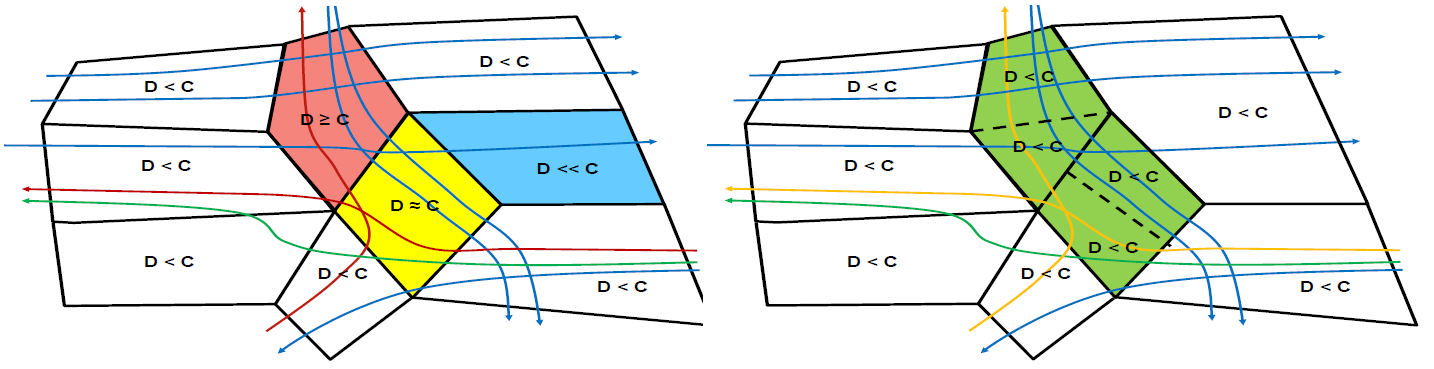
\includegraphics[width=1\textwidth]{\FIGDIR/02_02_DAM_Example}
    \caption{Example of DAM flight rerouting to homogenize traffic density \cite{gerdes2016dynamic}.}
    \label{fig:DAMExample}
\end{figure}

\begin{note}
    The air ways can not be changed, because the real time change of airways is difficult. The change of cluster authority is possible, because there is no changes for aircraft.
\end{note}

\noindent The airspace clusters are divined into three categories (fig. \ref{fig:DAMExample}):
\begin{enumerate}
    \item \emph{Under-fill} (blue) - there is less airplanes than its authority capacity.
    
    \item \emph{Saturated} (yellow) - there is enough airplanes to fill authority capacity.
    
    \item \emph{Over-fill} (red) - there is more airplanes than its authority capacity.
\end{enumerate}


\noindent The algorithm \cite{gerdes2016dynamic} will swap some airspace portions between neighbouring authorities to balance the load (all authorities should be saturated in ideal conditions) (green) (fig. \ref{fig:DAMExample}).
    	\subsection{(R) Airborne Collision Avoidance System X}\label{sec:ACASX}
\noindent This section follows the summary leaflet \cite{netalert2013n17}. The standard is still under development, the principles relevant for this work are outlined. 

\paragraph{Overview:} A development of \emph{ACAS-X} system is the FAA funded research and development program of a new approach to airborne collision avoidance. It has been ongoing since early 2008. ACAS-X approach takes an advantage of years of TCAS development. The main purpose of new system development is rapid evolution of computational capabilities and emergence of \emph{Unmanned Autonomous  Systems}.

The main purpose for manned aviation is to provide necessary advisories to pilot for \emph{Mid-Air Collision} (MAC) avoidance. There are following improvements:

\begin{enumerate}
    \item \emph{Reduce Unnecessary Advisories} - The pilot/UAS is receiving avoidance advisories or warning. 
    
    \item \emph{Extending collision avoidance to other classes of aircraft} - the current TCAS system is available mainly for bigger manned aviation, the future lies in integration of UAS systems into non-segregated airspace.
    
    \item \emph{Improvement of Surveillance Environment} - There is development in ADS-B technology and modern non cooperative sensors like LiDAR or milimeter radar, which are enhancing surviliance cappabilites of current and future airplanes.
\end{enumerate}

\paragraph{AcAS-X variants:} The \emph{ACAS-X} is not universal "\emph{one-size fits all}" system. There are multiple variations for different type of aviation:
\begin{enumerate}
    \item \emph{ACAS-X\textsubscript{P}} - the general purpose ACAS-X that makes active interrogations to establish the range of intruders. The successor to TCAS II.
    
    \item \emph{ACAS-X\textsubscript{P}} - a version of ACAS-X that relies solely on passive ADS-B to track intruders and does not make active interrogations. It is intended for general aviation (a class of aircraft not currently required to fit TCAS II).
    
    \item \emph{ACAS X\textsubscript{O}} - a mode of operation of ACAS X designed for particular operations for which ACAS-X\textsubscript{A} is unsuitable and might generate an unacceptable number of nuisance alerts (e.g. procedures with reduced separation, such as closely spaced parallel approaches).
    
    \item \emph{ACAS X\textsubscript{U}} - designed for \emph{Unmanned Aircraft Systems} (UAS).
\end{enumerate}

\begin{note}
    The \emph{ACAS X\textsubscript{U}} is mean also for \emph{reduced separation} approach in tightly packed airspace (ex. air-taxi). The determinism and \emph{false-positive} alerts occurrence minimization must be assured in order to enable UAS systems into non-segregated airspace.
\end{note}

\paragraph{ACAS-X Concept:} The \emph{ACAS-X} collision avoidance logic (fig. \ref{fig:acasxConceptScheme}) is distinguished into two phases:
\begin{itemize}
    \item[1.] \emph{Offline development phase} (Pre-calculation) similar to (sec. \ref{s:reachSet}) - ACAS-X is based on a \emph{probabilistic model} providing a statistical representation of the aircraft position in the future (position cone). It also takes into account the safety and operational objectives of the system (payload/weather/visibility/airspace/aircraft class). This enables the logic to be tailored to particular procedures or \emph{airspace configurations}.
    
    This is fed into an \emph{optimization process} called dynamic programming to determine the best course of action to follow according to the context of the conflict. This takes account of a reward (safety) to the cost (fuel consumption). The concurrent optimization enables to explore multiple maneuvers to determine which will increase \emph{separation level} (safety) and which will decrease \emph{fuel consumption} (cost).
    
    Key metrics for \emph{operational sustainability} and pilot acceptability include \emph{minimizing} the frequency of resolution advisories (UAS/GA) and traffic alerts (GA). This results into decrease of reversals/intentional intruder altitude crossing cases.
    
    \item[2.] \emph{Real-time operation} (Avoidance run) similar to (sec. \ref{s:missionControlRun}) - the \emph{look-up table} is used in real-time on-board the aircraft to resolve conflicts. An ACAS-X system collects \emph{surveillance measurements} form an array of \emph{information sources} and \emph{sensors}. The \emph{situation evaluation} is executed every second (decision time).
    
    Various models are used (e. g. a probabilistic sensor model accounting for sensor error characteristics) to estimate a state distribution, which is a probability distribution over the current positions and velocities of aircraft and intruders. The \emph{state distribution} determines where to look in the numeric look-up table to determine the best action to take. If deemed necessary \emph{Resolution Advisory} are issued to pilots/UAS control module.
    
\end{itemize}

\begin{figure}[H]
    \centering
    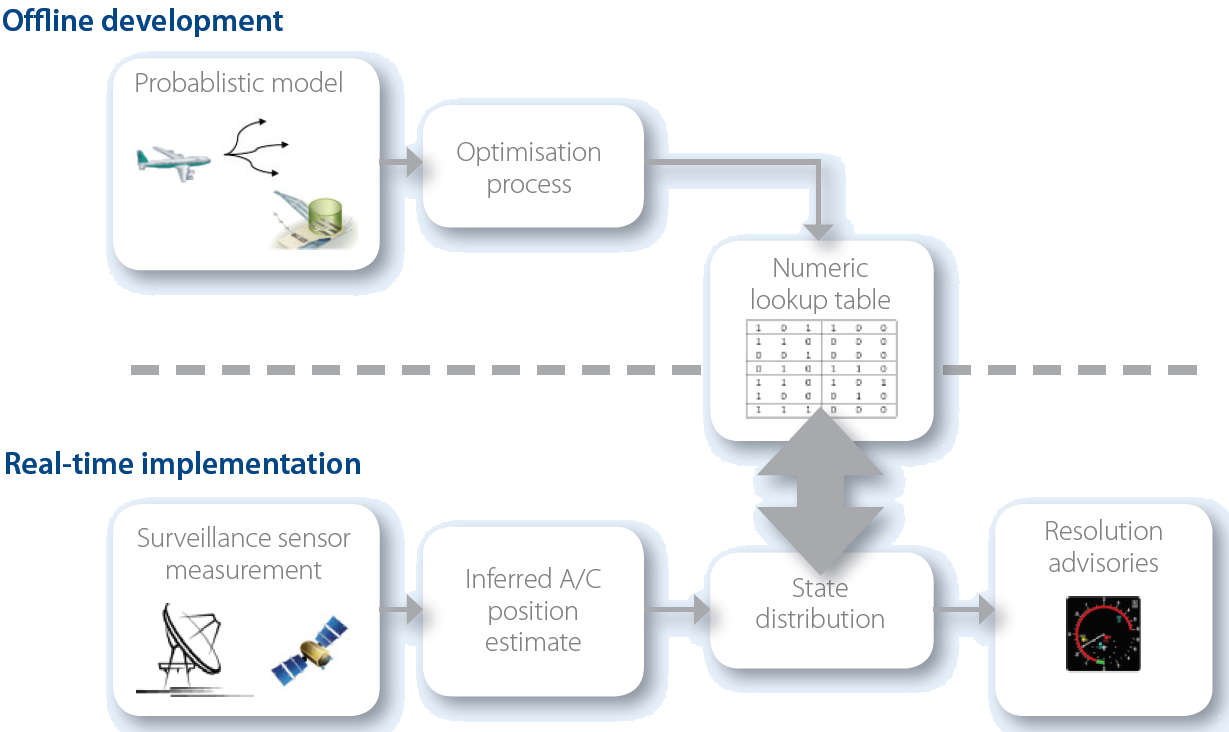
\includegraphics[width=.8\linewidth]{\FIGDIR/TE058TwoPhasesACASX}
    \caption{ACAS-X concept scheme \cite{netalert2013n17}.}
    \label{fig:acasxConceptScheme}
\end{figure}

\begin{note}
    \emph{Two-phase calculation} with offline development and real-time operation phase concept, will be used in different manner in our method. (sec. \ref{s:avoidanceConcept})
\end{note}

\paragraph{Advisories:} The \emph{ACAS-X} is taking the advisories categorization from \emph{ICAO Annex 10.} \cite{annex200710}. The advisories are recommended (directives for UAS) actions to take.


Airborne Collision Avoidance Systems (ACAS) equipment provides two types of advisories to pilots: Resolution Advisories (RAs) and Traffic Advisories (TAs). These are defined as follows:

\begin{enumerate}
    
    \item \emph{Resolution advisory} (RA) - an indication given to the flight crew recommending:
    
    \begin{enumerate}[a.]
        \item Manoeuvre intended to provide separation from all threats.
        
        \item Manoeuvre restriction intended to maintain existing separation.
    \end{enumerate}
    
    \item \emph{Corrective resolution advisory} - a resolution advisory that advises the pilot to deviate from the current flight path.
    
    \item \emph{Preventive resulution advisory} - a resolution advisory that advises the pilot to avoid certain deviations from the current flight path but does not require any change in the current flight path.

    \item \emph{Traffic advisory} (TA) - An indication given to the flight crew that a certain intruder is a potential threat.
\end{enumerate}

\begin{note}
    The \emph{UAS} system with full autonomy must handle the solution of the \emph{directives} (advisories) form UTM and other systems. The example of configurable handling mechanism - \emph{Rule engine} is given in (sec. \ref{s:RuleEngineArchitecture}).
\end{note}

\paragraph{Example Overview of the Incident:} The \emph{example of incident} and  a resolution is outlined in (fig. \ref{fig:axasxincidentoverviewexample}). The \emph{example} is given for better understanding of \emph{ACAS-X} roles \& responsibilities. 

\begin{itemize}
    \item[1.] \emph{Initial state} - the initial state is given like follow:
    
    \emph{Green Airplane} (A/C 1) is cruising on \emph{flight level} FL-390 (39 000 feet)
    
    \emph{Orange Airplane} (A/C 2) is cruising on \emph{flight level} FL-370 (37 000 feet)
    
    \item[2.] \emph{Orange aircraft transponder mishap} - the \emph{orange airplane} appears on flight level FL-405 (45 000 feet).  The \emph{green aircraft} controller (pilot) wants to \emph{descent} to oragne aircraft real flight level (FL-370). 
    
    \item[3.] \emph{Green airplane descent} - the \emph{Green aircraft} starts to descent. The \emph{Orange aircraft} keeps the flight level (FL-370). 
    
    \item[4.] \emph{Green aircraft Active Surveillance} - the \emph{green aircraft} uses \emph{active surveillance} to detect \emph{orange aircraft}. 
    
    The \emph{ACAS-X} issues \emph{Adjust Vertical Speed, Adjust - Resolution Advisory} (AVSA RA) to  the \emph{green aircraft} to \emph{level off} and stop \emph{descent} or at least slow it.
    
    Then as \emph{ACAS-X} issues \emph{Climb Resolution Advisory} to the \emph{green aircraft} mandating to get altitude. 
    
    \begin{note}
        The main issue is that \emph{pilot} is responsible decision maker, therefore pilot can refuse to follow \emph{ACAS-X advisories}.
    \end{note}
    
    \item[5.] \emph{Orange airplane starts descending} -  the \emph{orange aircraft} detects the \emph{flight level disparity} due the \emph{active surveliance} deteciton of \emph{green aircraft} on \emph{FL-370}.
    
    The \emph{Green aircraft} is tail-gating \emph{orange aircraft} from above. The \emph{ACAS-X} evaluates situation and issues a \emph{Descent Resolution Advisory} to avoid pursuit. 
    
    The \emph{pilot} of \emph{orange aircraft} follows the order of RA
\end{itemize}


\begin{figure}[H]
    \centering
    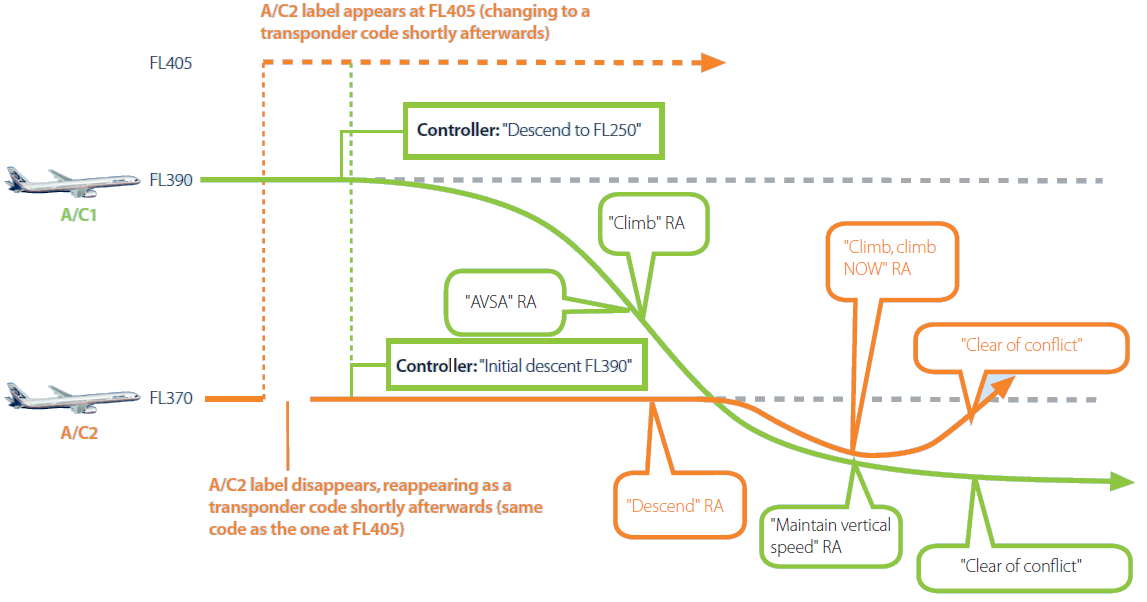
\includegraphics[width=\linewidth]{\FIGDIR/TE059ACASConflictExample}
    \caption{ACAS-X incident overview \cite{netalert2013n17}.}
    \label{fig:axasxincidentoverviewexample}
\end{figure}

\begin{itemize}
    \item[6.] \emph{Tailgating detection} - the \emph{orange airplane} is in front of \emph{green airplane}, both airplanes are descending at same rate. 
    
    \begin{note}
        This situation is very dangerous, because it is very close to \emph{intentional pursuit scenario}.
    \end{note}
    
    The \emph{orange airplane} is \emph{pursued}, its own \emph{ACAS-X} issues the \emph{Climb Now Resolution Advisory}. The pilot follows the advisory.
    
    The \emph{green airplane} is \emph{pursuing} and its goal is to \emph{descent} to flight level FL-250. Its \emph{ACAS-X} issues \emph{maintain vertical speed resolution advisory}.
    
    \item[7.] \emph{Conflict resolution} - both airplanes follow \emph{Resolution Advisories}.  When significant vertical distance is reached. The conflict is marked as resolved. 
\end{itemize}


    	\subsection{Traffic Collision Avoidance System}\label{sec:TCAS}

\noindent The \emph{TCAS} functionality is equal to ACAS-X\textsubscript{A} (sec. \ref{sec:ACASX}) functionality. The TCAS II. version 7.1 technical specification can be found in \cite{federal2011introduction}. A \emph{Resolution Advisory} (RA) detection algorithm is outlined in  \cite{munoz2013tcas}.
	
	%02-05 UTM section    
    \section{UAS Traffic Management (UTM)}\label{sec:UTM}
\paragraph{Introduction:} This section strongly follows \cite{eurocontrol2018rpasatm}, which outlined the basic concept of operations for Remotely Piloted Aerial Systems (RPAS)/Unmanned Autonomous Systems (UAS) Air Traffic Management (ATM) (later re-branded as UTM).

The \emph{RPAS/UAS} integration into \emph{non-segregated airspace} follows the general manned aviation procedure:
\begin{itemize}
    \item[$\to$] For a selected type of Operations VLOS/BVLOS/VFR/IFR:
    \begin{itemize}
        \item[$\to$] For a selected class of Air traffic (class 1. - class 7):
        \begin{itemize}
            \item[$\to$] For a selected class of airspace (class A -  class G):
            \begin{itemize}
                \item[$\to$] Deliver Operation Performance Standards ($\ge$ General Aviation)
            \end{itemize}
        \end{itemize}
    \end{itemize}
\end{itemize}

\noindent  The prototype of regulation for \emph{RPAS/UAS} standard from EASA can be found at \cite{easa2016rpasroperegul}. The section will continue with an outline of important functionality.

\paragraph{Airspace Assessment:} The future \emph{UTM} must be capable of \emph{airspace} assessment. In manned aviation, the \emph{airspace assessment} is normally triggered by either rise of traffic, environmental issues, capacity issues, and safety concerns or adapting the design to meet forecasted demands.

Presently RPAS/UAS operations have not triggered an airspace assessment s most areas are indicated as \emph{no RPAS/UAS zones}. The \emph{restricted areas} are already known on aviation maps (airport, nuclear power station, etc.). However, there are similarities with RPAS/UAS operations below 500 ft (AGL), that can trigger this requirement for an airspace assessment like, but not exclusive:

\begin{enumerate}
    \item \emph{The increase of operations density} - UAS taxi can lead to an increase in traffic density in class C and F airspaces, the UAS delivery system can lead to increased traffic density in F class airspace. 
    
    \item \emph{Introduction of BVLOS, autonomous VLOS/ELOS/BLOS operations} - current RPAS/ UAS operations are limited to VLOS which limits operation space. When this limitation is lifted, new business cases will open, leading to an \emph{increase} of RPAS/UAS traffic.
    
    \item \emph{Safety Concerns} - there is not enough accidents or critical RPAS/UAS misuse cases, to increase safety concerns, especially G class airspace does not have many manned aviation parallels.
    
    \item \emph{Environmental Aspect} - the RPAS/UAS is not constructed from clean and safe materials, any accident can lead to serious habitat damage (ex. gasoline in water reservoir).
\end{enumerate}

The \emph{assessment} should develop a new type of airspace organization able to cater to the new demand of operations and ensure safety levels are met. The airspace assessment can take into considerations the following aspects:

\begin{enumerate}
    \item \emph{Airspace classification} - further airspace decomposition in F/G  uncontrolled airspace to establish \emph{flight routes} and controlled areas. Further flight levels in C class airspace segmentation to enforce manned/unmanned aviation separation.
    
    \item \emph{Traffic complexity and density} - the \emph{congestion} of traffic is very common on the road. The capability to stop or stay still in the air is very costly to implement and maintain both in manned/unmanned aviation.
    
    \item \emph{Geographical situation} - flat-lands vs. mountains, urban vs. rural areas.
    
    \item \emph{Privacy} - in \emph{very low altitude} operations the privacy is always a concern.  The current restrictions to flew over private properties needs to be lifted in order to enable increased higher traffic density.
    
    \item \emph{Security} - the \emph{UTM} and \emph{RPAS/UAS} systems are creating a network of \emph{autonomous agents}; this network is venerable to any kind of \emph{cyber/physical} threat.
\end{enumerate}

\paragraph{Types of RPAS/UAS operations:} The \emph{future UTM functionality} must cover a wide range of functionality. It is envisaged that RPAS/UAS will operate in a mixed environment adhering to the requirements of the specified airspace it is operating in. RPAS/UAS will be able to operate as follows:

\begin{enumerate}
    \item \emph{Very Low-Level (VLL) operations} ($<500 feet (AGL)$).
    
    \item  \emph{IFR (Instrumental Flight Rules) or VFR (Visual Flight Rules)} ($500 feet \le altitude < 60 000 feet (AMSL)$) - following the same rules that apply to manned aircraft. These can be conducted in RLOS or B-RLOS conditions.
    
    \item  \emph{Very High-Level operations (VHL suborbital IFR operations above FL600)} ($\ge$ $60 000$ $feet$ $(AMSL)$).
\end{enumerate}

\paragraph{VLL operations (Below 500 feet AGL):} Operations performed at altitudes below 500 feet are not new to manned aviation as many operators - police, armed forces, balloons, gliders, training crafts, fire-fighting, ultra-light aircraft are allowed to operate in this environment. The rule allows VFR traffic to operate, under specific conditions prescribed by the competent national authorities, conditions that can differ from State to State. RPAS/UAS operating in this volume of airspace do not however confirm either IFR or VFR as given in ICAO Annex 2. \cite{icaoAnnex2}.

\begin{enumerate}
    \item \emph{VLOS (Visual Line Of Sight)} - RPAS/UAS operations within 500 meters range and max 500 feet  altitude from the a pilot. One of the main responsibilities of the pilot is the safe execution of the flight through visual means. The distance can be increased by the use of one or more observers, sometimes referred to as Extended-VLOS (E-VLOS).
    
    \item \emph{BVLOS (Beyond Visual Line Of Sight)} -  RPAS/UAS operations beyond 500 meters range but below 500ft. BVLOS does not require the operator to ensure the safety of the flight visually, and technical solutions such as DAA and C2 data link are required. RPAS/UTM does not adhere to VFR or IFR requirements; however, it is foreseen that these flights could be conducted in IMC or VMC conditions. BVLOS operations are already being conducted in several States. Some examples are:
    
    \begin{enumerate}[a.]
        \item Power-line control.
        
        \item Maritime surveillance.
        
        \item Pipeline control.
        
        \item  Agriculture.
    \end{enumerate}
\end{enumerate}

\noindent\emph{VLL Management System:} In order to accommodate the expected growth of traffic in this airspace and ensure a sufficient level of safety, it is anticipated the necessity for a supporting UTM system. This VLL Traffic Management system will provide a series of localization and information services, aiming to the provision of information to the RPAS pilots and manned traffic. The VLL UTM system will not provide an active control service for RPAS in a normal ATC fashion, due to a large number of RPAS/UAS involved. Such a system could be based on existing technologies, such as the mobile phone network. Specific RPAS/UAS reporting systems, providing authorization and information capability, are already in use in several states.

The RPAS/UAS management system will have to cater to the following aspects:

\begin{enumerate}
    \item  RPAS/UAS Flight planning.
    
    \item  RPAS/UAS Flight authorization.
    
    \item  Real-time RPAS/UAS tracking capability.
    
    \item  Provision of actual weather and aeronautical information.
\end{enumerate}

\noindent As previously mentioned, it is envisaged that the VLL management system will not support the active controlling of RPAS/UAS at lower altitudes. The large number of RPAS/UAS will not make this possible, notwithstanding any liability aspects. The system will be supporting operations and will be able to provide sufficient data to safely execute an RPAS/UAS flight, based on the information available to it. Data required could include, but are not limited to:

\begin{enumerate}
    \item Planned flight plans.

    \item Active RPAS/UAS flight plans/missions.

    \item Airspace data.

    \item NOTAM (NOtice To AirMan).
    
    \item Weather.

    %\item Infrastructure availability.

    \item Geo-fencing.

    \item Manned operations below 500 feet (AGL).
\end{enumerate}



\noindent The following assumptions have been made for future ATM/UTM systems:
\begin{enumerate}
    \item A C2 service is provided.

    \item The State has executed airspace, and assessment geo-fencing is in place.
    
    \item  RPAS/UAS have surveillance capability similar concerning performance and compatible to manned aircraft surveillance capability.
    
    \item  Specific RPAS/UAS traffic management system is in place.
\end{enumerate}

\begin{note}
    RPAS/UTM vehicle categorization is outlined in \emph{U-SPACE section} (sec. \ref{sec:USpace}).
\end{note}

\noindent The classification of traffic in this airspace segment goes like follow:


\paragraph{Class I.:} Class I traffic is primarily reserved for RPAS Category A (buy and fly). In areas of low traffic density this class can operate from the ground up to 500ft and is a subject to the following requirements:
    \begin{itemize}
        \item[1.]  Mandatory declaration of operation.
        
        \item[2.]  RPAS must be capable to self-separate in 3D.
        
        \item[3.]  VLOS operations only.
        
        \item[4.]  Geo-fencing capability which ensures that this category remains separated from no-drone zones.
    \end{itemize}
    
\paragraph{Class II.:} Class II traffic operates in free flight due to the nature of their operations like Surveys, filming, search and rescue and other operations that have no fixed route structure. Class II can operate from the ground up to 500 feet (AGL) and is a subject to the following requirements:
    \begin{itemize}
        \item[1.] Mandatory authorization for operation.
        
        \item[2.] Surveillance capability (C2 4G chip or other means).
        
        \item[3.] VLOS and BVLOS operations.
        
        \item[4.]  Free flight Capability.
        
        \item[5.]  RPAS/UAS must be capable to self-separate in 3D.
        
        \item[6.]  BVLOS will have barometric measurement equipage.
    \end{itemize}
    
    
\paragraph{Class III.:} Class III traffic only operates in BVLOS and is mainly used for transport purposes. It can operate as free flight or within a route structure pending on the requirements set by the airspace assessment.
    \begin{itemize}
        \item[1.] Mandatory authorization for operation.
        
        \item[2.] Has surveillance capability.
        
        \item[3.] BVLOS operations only.
        
        \item[4.] Free flight or route structure.
        
        \item[5.] Shall have barometric measurement equipage.
        
        \item[6.] Can operate from the ground up to 500 ft.
    \end{itemize}
    
\paragraph{Class IV.:} Class IV traffic can operate within the layer between the ground and 500 feet. This category is designed for highly specialized operations and as such not many of these types RPAS/UAS are expected. These can be civil, state or military operations and as such:
    \begin{itemize}
        \item[1.] Require special authorization.
        
        \item[2.] Should be addressed on a case by case basis.
        
        \item[3.] VLOS and BVLOS.
        
        \item[4.] Could require surveillance capability.
    \end{itemize}

\paragraph{IFR/VFR Operations (between 500ft - FL 600):} For RPAS/UAS to fly either IFR/VFR requires that they meet the airspace requirements as set for manned aviation. These operations include airports, TMA and Enroute. For IFR capable RPAS additional requirements can be set for flying in the volumes of airspace where normal transport aircraft operate. As such it is envisaged to have minimum performance standards for elements such as speed, climb/descent speed, turn performance and latency.

\emph{Operations of Small RPAS above 500 feet:} In principle operations above 500 feet by small RPAS/UAS are not allowed unless they meet the IFR/VFR airspace requirements and have a solution to be visible to manned traffic. Other aspects like wake turbulence and separation standards would also have to be addressed. However, States can still on a case by case basis accommodate RPAS/UAS above 500ft if the risk assessment of the intended operation is acceptably low.

\noindent The classification of traffic in this airspace segment goes like follow:

\paragraph{Class V.:} Class V is IFR/VFR operations outside the Network not flying SIDs and STARs. In this environment, RPAS/UAS not meeting Network performance requirements will be able to operate without negatively impacting manned aviation. Operations at airports will be accommodated through segregation of launch and recovery.

    Ground operations can also be accommodated through either towing or wing walking.

    Operations from uncontrolled airports or dedicated launch and recovery sites are to be conducted initially under VLOS/VFR until establishing radio contact with ATC.

    No additional performance requirements will be set in this environment compared to manned aviation.
    
    RPAS/UAS operating in the environment will file a flight plan including information such as:
    \begin{itemize}
        \item[1.] Type of RPAS/UAS, 2. Mission plan, 3. Contingency procedure.
        
        \item[4.] RPAS/UAS will meet CNS airspace requirements.
        
        \item[5.] RPAS/UAS will be able to establish two-way communication with ATC/UTM if required.
        
        \item[6.]  RPAS/UTM will remain clear of manned aircraft.
        
        \item[7.]  RPAS operator must be able to contact ATC/UTM (if required) regarding special conditions such as data link loss, emergency, controlled termination of flight.
        
        \item[8.] RPA/UTM DAA capability will be cooperative with existing ACAS systems.
    \end{itemize}
    
\paragraph{Class VI.:} Class VI. is IFR operations, including Network, TMA and Airport operations with RPAS/UAS capable of flying SIDs and STARs as designed for manned operations. These are either manned transport aircraft enabled to fly unmanned with similar capabilities or new types able to meet the set performance requirements for the Network, TMA and airports. General requirements RPAS/UAS operating in this environment will file a flight plan (mission) including:
    \begin{itemize}
        \item[1.] Type of RPAS/UAS.
        \item[2.] Contingency procedure.
        \item[3.] Mission plan (navigation, route, level).
        \item[4.] RPAS/UAS will meet CNS airspace requirements.
        \item[5.] RPAS/UAS will be able to establish two-way communication with ATC/UTM.
        \item[6.] RPAS/UAS operator must be able to contact ATC (if required) in regard regarding special conditions such as data link loss, emergency, controlled termination of flight.
        \item[7.] RPAS/UAS DAA capability will have ACAS functionality.
    \end{itemize}

\begin{note}
    The class operation class $V.-VI.$ is covered mostly in this work.
\end{note}

\paragraph{VHL operations (Above FL 600):} Suborbital unmanned flights operating at altitudes above FL 600 are expected to grow fast in numbers. Apart from military HALE RPAS, several other vehicles (i.e., space rockets, Virgin Galactic, etc.) operate through or in this block of airspace. At this moment, no management of this traffic is foreseen in most parts of the world. Particular attention should be given to the entry and exit of this high altitude volume as they need to interact with the airspace below.

\noindent The classification of traffic in this airspace segment goes like follow:


\paragraph{Class VII.:} Class VII consists solely of IFR operations above FL600 and transiting non-segregated airspace.
    
    These types of RPAS/UAS are solely designed for operations at very high altitudes. The launch and recovery of fixed-wing RPAS/UAS can be from dedicated airports and outside congested airspace unless Class VI requirements are met. This airspace will be shared with many different RPAS/UAS. Although their operations will not directly impact the lower airspace, however, they will have to transit through either segregated or non-segregated airspace to enter or exit the airspace above FL 600.
    
    For such cases, temporary segregated airspace should be considered. Transition performance in segregated or non-segregated airspace below FL600 will be very limited since they will be focusing on long missions (up to several months).

    The airspace in which these types of operation take place is mostly seen as uncontrolled. This requires no management of this traffic; however due to the expected numbers - estimated to be around 18000 just for Google and Facebook - it will become necessary to manage this type of operation since the performance envelopes differ a lot. Speeds can vary from average wind speed at those altitudes (for Google balloons) up to above-mach.

    Launch and recovery of unmanned balloons or aircraft, together with emergency situations, will also require a set of procedures and pre-arranged coordination capabilities to ensure the safety of traffic below this altitude.



    	\subsection{U-Space}\label{sec:USpace}

\noindent The \emph{Concept Of OpeRations of U-Space} (CORUS) \cite{corus2018} has been released recently. This concept describes the difference between the standard ATM and proposed European UTM solution. This section will get through the interesting part of this pivotal document.

\newpage\noindent The \emph{U-space} is separated into following functionality based phases:
\begin{itemize}
    \item[\texttt{U1}] (year $<$ 2020) - sets the scene with registration and geo-fencing.
    
    \item[\texttt{U2}] (year$<$ 2025) - introduces tracking, flight planning and messages sent to the remote pilot during flight.
    
    \item[\texttt{U3}] (year$<$ 2030) introduces collaborative detect and avoid and tactical conflict resolution.
    
    \item[\texttt{U4}] (year $<$ 2035) brings safe interoperation with manned aviation.
\end{itemize}

The \emph{Aspects} important for \emph{Obstacle avoidance} will be outlined and discussed over this section. Our work focuses on \emph{European Airspace} (EASA); therefore more focus will be on \emph{U-space}

\paragraph{Small UAS Classification:} Manned aviation is covered by existing rules, for example \cite{icaoAnnex2,ec201208ref5}. Excluding some specific situations, manned aviation does not fly below VFR airspace, do not enter \emph{very low level} (VLL) altitudes \cite{ec200802ref4}. 

The certified airworthiness is mandatory for \emph{airspace attendants} with \emph{Maximum Take-Off Mass} (MTOM) over $150 kg$. The other \emph{airspace attendants} need to fulfill only \emph{Minimal Operation Performance Specification} (MOPS). 

In \cite{easa201801op} EASA proposed several classes for UAS below $150kg$ MTOM; see Appendix 1 of the annex to Opinion 1-2018 entitled "…on making available on the market of unmanned aircraft intended for use in the ‘open’ category" and on third-country UAS operators. In that text, the next smaller mass mentioned below 150kg is 25kg MTOM. A similar break is proposed in some national legislation, for example in the UK at 20kg. As a working definition, this little chart shows a possible breakdown by MTOM. Note
that EASA classes depend on many factors, not only MTOM.

\begin{table}[H]
    \centering
    \begin{tabular}{c||c|l}
    \begin{tabular}[c]{@{}c@{}}EASA\\ class\end{tabular} & \begin{tabular}[c]{@{}c@{}}Maximum \\ take-off mass\end{tabular} & Remarks \\\hline\hline
     C0 & $\le 250 g$   & "Child`s Toy" with very limited capabilities \\\hline
     C1 & $\le 900 g$   & "Adult`s Toy" small flying camera \\\hline
     C2 & $\le 4 kg$    & "Small UAS" with the package \\\hline
     C3 & $\le 25 kg$   & "Standard UAS" attainable AGL altitude $\le 120m$ \\\hline
     C4 & $\le 25 kg$   & "Standard UAS" no automatic control mode  altitude $> 120m$\\\hline
     -  & $\le 150 kg$  & "Heavy UAS", not defined in \cite{easa201801op} \\\hline
     -  & $> 150 kg kg$ & Regulated by EASA like the manned aircraft \cite{ec200802ref4} 
    \end{tabular}
    \caption{Small UAS Classes according to EASA. \cite{corus2018}}
    \label{tab:smallDroneClessesAccordingtoEASA}
\end{table}

\begin{note}
    The class C3 and C4 are different in operational restrictions. This work focuses mainly on UAS classes C2/C3/C4 because they have enabled \emph{automatic control mode} 
\end{note}
\newpage
\paragraph{Separation Minima:} The \emph{Separation Minima} defines \emph{minimal distances} between airspace attendants to ensure secure \emph{operation}.  The separation minima are taken from Corus \cite{corus2018}. 

All ideas for safe concurrent operation of UAS are based on the idea of keeping the UAS systems apart or physically distant from some risk source. 

A geo-fence, for example, is simply a method of providing separation. There will need to be separation minima for UAS just as there are for manned aircraft and these will be needed by services such as Monitoring which seeks to warn about loss of separation and Tactical Conflict Resolution which may act to avoid the loss of separation.

Separation minima will be different from those for manned aircraft as small UAS systems are generally much smaller and often slower moving than manned aircraft. CORUS proposes the following as separation minima (tab. \ref{tab:proposedseparationMinimaforUAS})

\begin{table}[H]
    \centering
    \begin{tabular}{l||l|l|l}
        \multicolumn{1}{c||}{\begin{tabular}[c]{@{}c@{}}Flight Type\\ Interaction\end{tabular}} & \multicolumn{1}{c|}{Horizontal} & \multicolumn{1}{c|}{Vertical|} & \multicolumn{1}{c}{Remark} \\\hline\hline
        %TableLine 1
        \begin{tabular}[c]{@{}l@{}}
            Any UAS - Manned or\\
            person carrying
        \end{tabular} & 
        \begin{tabular}[c]{@{}l@{}}
            2.5 NM
        \end{tabular} & 
        \begin{tabular}[c]{@{}l@{}}
            500 ft
        \end{tabular} & 
        \begin{tabular}[c]{@{}l@{}}
            Half the current manned\\
            aircraft separation
        \end{tabular}\\\hline
        
        %TableLine 2
        \begin{tabular}[c]{@{}l@{}}
            VLOS - VLOS
        \end{tabular} & 
        \begin{tabular}[c]{@{}l@{}}
            Remain\\
            "Well Clear"
        \end{tabular} & 
        \begin{tabular}[c]{@{}l@{}}
            Remain\\
            "Well Clear"
        \end{tabular} & 
        \begin{tabular}[c]{@{}l@{}}
            The remote pilot is not\\
            expected to judge distance by\\
            sight from the remote piloting\\
            position.
        \end{tabular}\\\hline
        
        %TableLine 3
        \begin{tabular}[c]{@{}l@{}}
            VLOS - BVLOS
        \end{tabular} & 
        \begin{tabular}[c]{@{}l@{}}
            Remain\\
            "Well Clear"\\
            + 200 ft
        \end{tabular} & 
        \begin{tabular}[c]{@{}l@{}}
            Remain\\
            "Well Clear"\\
            + 200 ft
        \end{tabular} & 
        \begin{tabular}[c]{@{}l@{}}
            The remote pilot is not\\
            expected to judge distance by\\
            sight from the remote piloting\\
            position.
        \end{tabular}\\\hline
        %TableLine
        \begin{tabular}[c]{@{}l@{}}
            BVLOS – BVLOS
        \end{tabular} & 
        \begin{tabular}[c]{@{}l@{}}
            200 ft
        \end{tabular} & 
        \begin{tabular}[c]{@{}l@{}}
            150 ft
        \end{tabular} & 
        \begin{tabular}[c]{@{}l@{}}
            Figures come from a \\
            pessimistic estimate of\\
            satellite navigation\\
            performance.
        \end{tabular}
\end{tabular}
    \caption{Proposed separation minima for UAS. \cite{corus2018}}
    \label{tab:proposedseparationMinimaforUAS}
\end{table}

\begin{note}
    The \emph{BVLOS – BVLOS} separation minima are interesting because the \emph{autonomous mode} is considered as BVLOS to  BVLOS avoidance in case of autonomous UAS.
    
    The \emph{separation minima} for \emph{UAS - Manned aviation} is unreasonably huge (2 nautical miles), and in current it should be considered as moving constraint.
\end{note}

\newpage
\paragraph{Flight Rules:} The \emph{aspects} of UAS flight rules for U-SPACE concept is summarized in the table:
\begin{table}[H]
    \centering
    \begin{tabular}{l||l}
        \multicolumn{1}{c||}{
        \begin{tabular}[c]{@{}c@{}}
            Aspect
        \end{tabular}} & 
        %\multicolumn{1}{c}{Hobby Flight Rules} &
        \multicolumn{1}{c}{UAS Flight Rules} \\\hline\hline
        %riadok 1
        \begin{tabular}[c]{@{}l@{}}
            Flight plan required
        \end{tabular} & 
        %\begin{tabular}[c]{@{}l@{}}
        %    No, but allowed
        %\end{tabular} & 
        \begin{tabular}[c]{@{}l@{}}
            Yes
        \end{tabular}\\\hline
        %riadok 2
        \begin{tabular}[c]{@{}l@{}}
            Allowed flight type
        \end{tabular} & 
        %\begin{tabular}[c]{@{}l@{}}
        %    VLOS, EVLOS
        %\end{tabular} & 
        \begin{tabular}[c]{@{}l@{}}
            VLOS, EVLOS, BVLOS
        \end{tabular}\\\hline
        %riadok 3
        \begin{tabular}[c]{@{}l@{}}
            Provision of separation in U1,\\
            VLOS \& EVLOS
        \end{tabular} & 
        %\begin{tabular}[c]{@{}l@{}}
        %    Pilot
        %\end{tabular} & 
        \begin{tabular}[c]{@{}l@{}}
            Pilot
        \end{tabular}\\\hline
        %riadok 4
        \begin{tabular}[c]{@{}l@{}}
            Provision of separation in U1,\\
            BVLOS
        \end{tabular} & 
        %\begin{tabular}[c]{@{}l@{}}
        %    N/A
        %\end{tabular} & 
        \begin{tabular}[c]{@{}l@{}}
            Geo-fence / Geo-cage
        \end{tabular}\\\hline
        %riadok 5
        \begin{tabular}[c]{@{}l@{}}
            Provision of separation in U2
        \end{tabular} & 
        %\begin{tabular}[c]{@{}r@{}l@{}}
        %    1. & Pilot (visual)\\
        %    2. & Limited support may be\\
        %       & obtained by using a Traffic\\
        %       & Information Service\\
        %\end{tabular} & 
        \begin{tabular}[c]{@{}r@{}l@{}}
            1. &  Strategic Conflict Resolution\\
               &  enabled by flight planning\\
            2. &  Traffic Information Service\\
               &  enabled by position reporting\\
            3. &  Pilot (visual)\\
        \end{tabular}\\\hline
        %riadok 6
        \begin{tabular}[c]{@{}l@{}}
            Provision of separation in U3 \&\\
            U4
        \end{tabular} & 
        \begin{tabular}[c]{@{}r@{}l@{}}
            1. &   Strategic Conflict Resolution\\
               &   enabled by flight planning\\
            2. &   Traffic Information Service\\
               &   enabled by position reporting\\
            3. &   Cooperative Tactical\\
               &   Conflict Resolution\\
            4. &   Detect and Avoid\\
            5. &   Pilot (visual)
        \end{tabular}\\\hline
        %riadok 7
        \begin{tabular}[c]{@{}l@{}}
            Separation from manned\\
            aviation in U2, VLOS or EVLOS\\
            UAS flight
        \end{tabular} & 
        \begin{tabular}[c]{@{}l@{}}
            The pilot is responsible\\
            to get the UAS out of the way\\
            of the manned aircraft.\\
        \end{tabular}\\\hline
        %riadok 8
        \begin{tabular}[c]{@{}l@{}}
            Separation from manned\\
            aviation in U2, BVLOS UAS\\
            flight\\
        \end{tabular} & 
        \begin{tabular}[c]{@{}l@{}}
            Flight plan required from both.\\
            Separation by planning.\\
            BVLOS pilot should use traffic\\
            information to avoid the\\
            manned aircraft (which is\\
            tracked).
        \end{tabular}\\
    \end{tabular}
    \caption{Aspects of UAS flight rules.\cite{corus2018}}
    \label{tab:aspectsOfUasFlightRules}
\end{table}

\noindent Following \emph{detect and avoid} requirements can be outlined based on (tab. \ref{tab:aspectsOfUasFlightRules}).
\begin{enumerate}
    \item \emph{Separation in U1} - only \emph{identification services} are provided in this phase. The \emph{Detect And Avoid} support can be provided only to UAS pilot in the form of visual or sound advisories. 
    
    \item \emph{Separation in U2} - the \emph{position notifications} are added, enabling, preemptive collision avoidance by flight planning (mission control). The \emph{traffic information} can be added to pilot software for better situation awareness.  


    \item \emph{Separation in U3 \& U4} - the \emph{advanced} avoidance concepts, from our perspective following aspects are interesting: 
    \begin{enumerate}[a]
        \item \emph{Cooperative Tactical Conflict Resolution} - The UTM infrastructure and hierarchy for \emph{cooperative conflict} resolution must be established. In form of UTM \emph{directives} and UAS \emph{fulfillment}.
        
        \item \emph{Detect and Avoid} - reactive obstacle/intruder avoidance and situation awareness on a very high level.
    \end{enumerate}
    
    \item \emph{Separation from Manned Aviation} - the \emph{well clear threshold} (fig. \ref{fig:WellClearTreshold}) for manned aviation  (tab.\ref{tab:proposedseparationMinimaforUAS}) are too big. The \emph{effective} application of \emph{reactive obstacle avoidance} is not reasonable, because the manned aviation will be out of range for most sensors (except ADS-B).
\end{enumerate}

\begin{note}
    Our work covers \emph{cooperative conflict resolution} and \emph{detect \& avoid}.
\end{note}

\paragraph{Geo-fencing Modes:} A Geo-fencing appears in U1, U2, and U3 and is successively refined. It is supported by aeronautical information for UAS systems. This table summarizes the different features by level:

\begin{table}[H]
    \centering
    \begin{tabular}{l||l|l}
        \multicolumn{1}{c||}{Capability} & \multicolumn{1}{c|}{Level} & \multicolumn{1}{c}{Features} \\\hline\hline
        %line 1
        \begin{tabular}[c]{@{}l@{}}
            Pre-Tactical \\Geo-Fencing
        \end{tabular} & 
        \begin{tabular}[c]{@{}l@{}}
            U1
        \end{tabular} & 
        \begin{tabular}[c]{@{}l@{}}
            Information provided before flight. The user should have\\
            access to AIP and NOTAM defined geo-fences in a form that\\
            can be used when planning and that can be loaded onto the\\
            UAS if it has geo-fence fence features in its navigation\\
            system
        \end{tabular}\\\hline
        %line 2
        \begin{tabular}[c]{@{}l@{}}
            On-board \\Geo-Fencing
        \end{tabular} & 
        \begin{tabular}[c]{@{}l@{}}
            U1
        \end{tabular} & 
        \begin{tabular}[c]{@{}l@{}}
            The ability of the UAS to keep itself on the correct side of a\\
            geo-fence by having geo-fence definitions (location, time,\\
            height) within its navigation system\\
        \end{tabular}\\\hline
        %line
        \begin{tabular}[c]{@{}l@{}}
            Tactical \\Geo-Fencing
        \end{tabular} & 
        \begin{tabular}[c]{@{}l@{}}
            U2
        \end{tabular} & 
        \begin{tabular}[c]{@{}l@{}}
            This service delivers to the pilot and /or UAS operator\\
            updates to and new definitions of Geo-Fences occurring at\\
            any time, including during flight.\\
            The creation of geo-fences with immediate effect require\\
            that they are defined outside the AIP. 
        \end{tabular}\\\hline
        %line
        \begin{tabular}[c]{@{}l@{}}
            UAS \\Aeronautical\\
            Information\\ Management
        \end{tabular} & 
        \begin{tabular}[c]{@{}l@{}}
            U2
        \end{tabular} & 
        \begin{tabular}[c]{@{}l@{}}
            U2 include a non-AIP repository of Geo-Fences. The\\
            UAS Aeronautical Information Management service\\
            includes all information coming from such a source,\\
            combined with information from the AIP and NOTAMS\\
            together with any other UAS relevant sources.
        \end{tabular}\\\hline
        %line
        \begin{tabular}[c]{@{}l@{}}
            Dynamic\\Geo-Fencing
        \end{tabular} & 
        \begin{tabular}[c]{@{}l@{}}
            U3
        \end{tabular} & 
        \begin{tabular}[c]{@{}l@{}}
            This service delivers updates definitions of geo-fences\\
            directly into the UAS, even in flight. This service\\
            relies on capabilities of the UAS in U3 to receive\\
            communications from U-space and to deal with geo-fence\\
            updates.
        \end{tabular}
    \end{tabular}
    \caption{Geo-fencing in U-space. \cite{corus2018}}
    \label{tab:geofencingInUspace}
\end{table}

\noindent The \emph{impact of geo-fencing} on \emph{Detect and Avoid} system is following:
\begin{enumerate}
    \item \emph{Pre tactical} - The \emph{flight plan} (mission) is prepared to avoid all \emph{known forbidden areas}. In this phase, the geo-fence covers static space constraints.
    
    \item \emph{Onboard} - The \emph{flight plan} (mission) specification does not contain all static space constraints. These constraints are known prior the flight. If UAS approaches such constraints, it needs to avoid them. The concept of soft constraints - restricted, but breakable space constraints emerge. 
    
    \item \emph{Tactical} - The \emph{space constraints} are updated during the flight. This can also be used for notifying the weather situations, restricted airspace, and all sort of \emph{static or moving constraints}.
    
    \item \emph{Dynamic} - The \emph{space constraints} the updates are real time.
\end{enumerate}

\begin{note}
    The work covers dynamic and tactical \emph{Geo-fencing}.
\end{note}

\paragraph{Actively maintaining separation during flight:} The standard ATM functionality \cite{icao4444} and \emph{Rules Of the Air} \cite{icaoAnnex2,icaoAnnex11} are covered and to be implemented for \emph{U-Space}.
    	\subsection{\secState{R}NASA UTM}\label{sec:NASAUtm}

\noindent The \emph{NASA UTM}\footnote{Related research and articles: \url{https://utm.arc.nasa.gov/documents.shtml}} is UAS Traffic Concept developed by \emph{National Aeronautics and Space Administration} (NASA) in cooperation \emph{Federal Aviation Administration} (FAA). The \emph{concept} is very similar to \emph{EASA U-SPACE}.

\begin{note}
    This work is focused on \emph{European Airspace}; the \emph{details} will be omitted. 
\end{note}

\paragraph{Useful concepts:} The \emph{NASA UTM} concept has greater maturity level concerning \emph{Detect \& Avoid} concept than European \emph{U-Space}. There is vast amount of publications which can be used in \emph{U-Space} from these publications the following useful studies containing DAA concepts were taken into account:

\begin{enumerate}    
    \item The non-cooperative intruder avoidance concept \cite{cone2017uas} provides a general idea about the \emph{topic}. The \emph{vertical separation} and \emph{vertical encounter model} is presented.
    
    \item The \emph{Detect and Avoid} performance evaluation is crucial for system performance assessment. The assessment framework \cite{lee2016wide} provides us with methodological guidelines. The used concepts are abstracting the multidimensional performance criteria into simple metrics:
    
    \begin{enumerate}[a.]
        \item \emph{Crash Distance} - the distance to the obstacle/intruder margin.
        
        \item \emph{Safety Margin} - the virtual margin around obstacle/intruder.
    \end{enumerate}
    
    \item To \emph{Ensure} the compatibility between \emph{UAS Detect And Avoid System} and \emph{Manned Aviation Collision Avoidance} (ACAS/TCAS) systems the following approach was proposed \cite{thipphavong2017ensuring}.
\end{enumerate}

    	
    %02-06 Event Based Avoidance
    \section{(W) Event Based Avoidance}\label{sec:EventBasedAvoidance}
\begin{itemize}
    \item Introduce the context for Event based avoidance: 
    \begin{itemize}
        \item Preventive DAA - before flight preparation
        \item Event-based DAA - reaction window in minutes, usually cooperative via notifications and other methods
        \item Reactive DAA - you know the drill boys ..., reaction window in 10th of seconds ...
    \end{itemize}
    \item Introduce the process of notification and Event Resolution
    \item Outline hierarchy in U(A)TM controlled space 
    \item Outline expected minimal set of data sources
\end{itemize}

\subsection{(W) Mid-Air Collision Prevention}\label{sec:MidairCollisionPrevention}
\begin{itemize}
    \item Identify and dispute shortcomings of Aircraft classification in ICAO
    \item List of MAC events
    \item For each event describe trigger and resolution 
    \item cite barrel \cite{welzl1991smallest}
\end{itemize}

\subsection{(W) Weather Impact}\label{sec:WeatherImpact}

    \begin{itemize}
        \item do not use term "climate change"
        \item critical events are getting more localized and their magnitude is increased
        \item List of Weather event
        \item Discuss weather mitigation
    \end{itemize}
    
    \emph{Weather Impact} on transportation in general has been introduced by Koetse in study \cite{koetse2009impact}.
    
    \emph{Weather-based} preemptive planning have been introduced into manned aviation in 2015 \cite{yamashita2015climate}. \TBD{This one shows global model impact}
    
    \emph{Severe Weather Condition Detection Capabilities} for current level of standard aviation equipment have been reviewed in \cite{smith2016multi} \TBD{This one shows intermediate weather detection}
    
    \begin{figure}[H]
	\centering
	\begin{subfigure}{0.45\textwidth}
		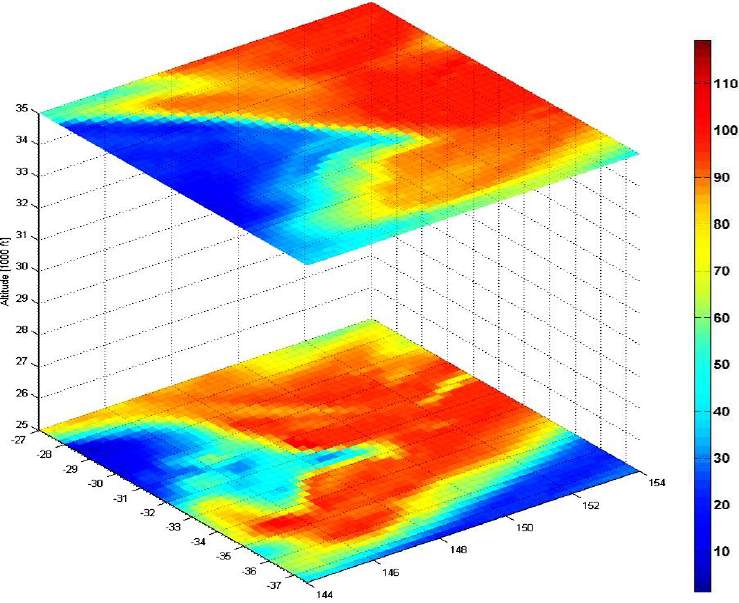
\includegraphics[width=\textwidth]{\FIGDIR/02_03_RelativeHumidity}
		\caption{Relative Humidity.} 
	\end{subfigure}
	\vspace{1em} 
	\begin{subfigure}{0.45\textwidth} % width of right subfigure
		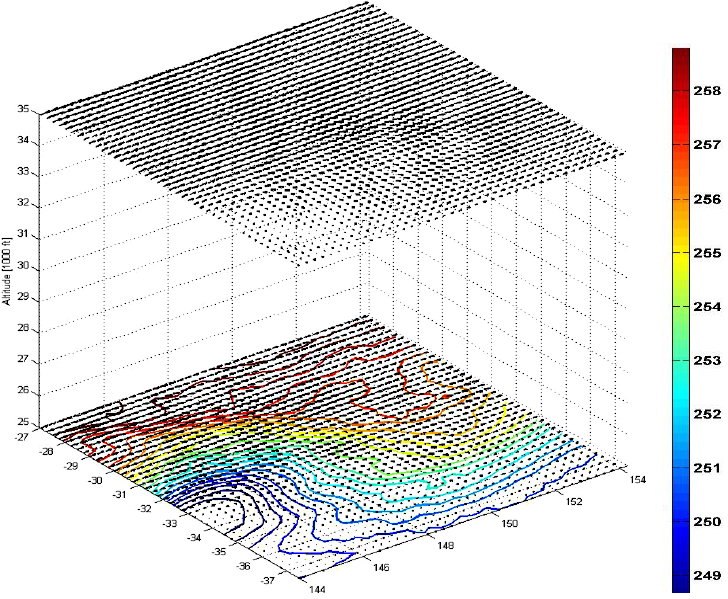
\includegraphics[width=\textwidth]{\FIGDIR/02_04_WindTemperature}
		\caption{Localized Wind Vectors.} % subcaption
	\end{subfigure}
	\caption{Localized Weather Model \cite{balaban2017dynamic}.} % caption for whole figure
    \end{figure}
    
    \emph{Icing risk} in localized environment have been predicted based on numerical model \cite{thompson2017numerical}. It is shown that icing can be prevented by \emph{planned} and \emph{reactive} avoidance.
    
    \emph{Weather Models} can be extracted from \emph{Climate and weather model archive at the National Oceanic and Atmospheric Administration} \cite{rutledge2006nomads}.
    
    \begin{figure}[H]
        \centering
        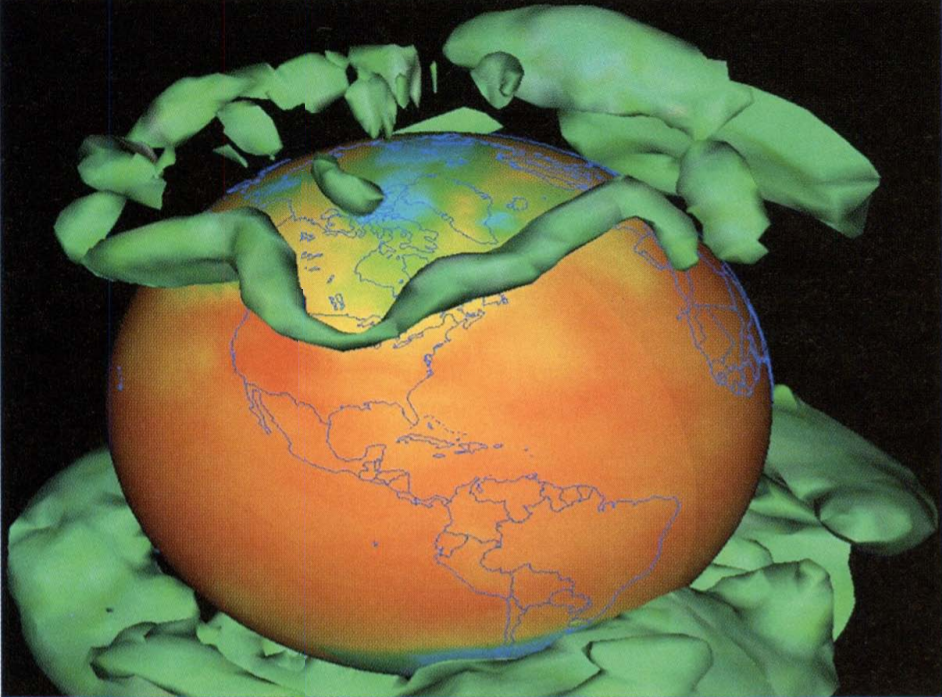
\includegraphics[width=0.7\textwidth]{\FIGDIR/02_01_IVS_Model}
        \caption{Example of upper troposphere winds \cite{rutledge2006nomads}.}
        \label{fig:ExampleOfTroposphereWinds}
    \end{figure}


    \subsection{(R) Mid-Air Collision Prevention}\label{sec:MidairCollisionPrevention}
\paragraph{Idea:} The first fatal mid-air collision occurred in 1912. The occurrence rate increased with technological progress. The \emph{European airspace management} is thoroughly analyzed in \cite{cook2007european}. 

\emph{Mid-Air Collision Situations:} The most common situations when \emph{Mid Air Collision} occurs are:

\begin{enumerate}
    \item \emph{Approach} (airport landing sequence) - the traffic density is increasing with proximity to traffic hub (airport). The aircraft lowers velocity in early approach phase to critical level which significantly reduces maneuverability. The \emph{final approach} phase is most dangerous, because the aircraft is close to the ground prepare to the landing.  
    
    \item \emph{Descent} (decrease of altitude) - the pilot is heading plane down, the dead angle is much greater than in other situations.
    
    \item \emph{Cruise}  (keeping same altitude) - the pilot is  keeping the altitude and heading, the awareness usually decreases significantly in this slight phase. 

    \item \emph{Climb} (increase of altitude) - the pilot is heading plane up, the dead angle is increased significantly. 
\end{enumerate}

\begin{note}
    The \emph{Mid-Air Collision} occurrence is strongly correlating with \emph{traffic density}. Therefore the most of \emph{near miss /collision cases} happens in vicinity of airport. It is expected to elevate the risk of \emph{Mid-Air Collision} by enabling \emph{UAS} into \emph{B, C, D, airports class}  airspace.
\end{note}

\paragraph{Collision Situation Awareness:} The surveillance capability of manned aviation is limited by \emph{pilot`s field of vision} in case of VFR (sec. \ref{sec:VisualFlightRules}) and by \emph{technical limitations} in case of IFR (sec. \ref{sec:InstrumentalFlightRules}). The \emph{surveillance and avoidance} support systems like TCAS (sec. \ref{sec:TCAS}) and ACAS (sec. \ref{sec:ACASX}) can be used as a base of future \emph{DAA} system.

The \emph{UAS} collision situation awareness system is taking the \emph{mid-air} collision prevention to another level, additional functionality needs to be implemented:

\begin{enumerate}
    \item \emph{Intruder trajectory prediction} - anticipate future \emph{intruder actions} based on gathered knowledge. Recognize dangerous actions or triggering situations. The triggering events of future dangerous situations are processed by pilot in manned aviation.
    
    \item \emph{Intruder intersection model} - anticipate future maneuverability and physical properties (turbulence, body size) in intersection model of the intruder and try to estimate an impact area in future. This process is done by pilot in manned aviation. Some supplementary information like \emph{aircraft type} and some properties are provided by surveillance system. The final decision and estimate needs to be automatized in form of impact probability or impact rating. 
    
    \item \emph{Decision making process} - the situation assessment gives an outline of the surrounding space properties, this process is well covered by \emph{surveillance}. The decision making process needs to be flexible and adaptable, but the limited computational resources needs to be taken into account (discretization problem).
\end{enumerate}

\begin{note}
    The \emph{example} of \emph{enclosed operational space} which is necessary for \emph{intruder intersection} detection is given in \cite{welzl1991smallest}.
\end{note}
    \subsection{\secState{R}Weather Impact}\label{sec:WeatherImpact}

\paragraph{Idea:} The \emph{climate} have stable properties over the course of the year. There are observations that climate is shifting in Europe, the periods of sprint/autumn weather are shortening, the periods of summer and winter are prolonging. 

Overall the \emph{European Climate} is getting similar to \emph{North America`s} continental climate. This has severe impact on many aspects of modern society including transportation, specially aviation, emerging UAS industry. 

The key fact is that occurrence of critical weather conditions, like storms or heavy winds is increasing. Along with increasing intensity of these events, the magnitude increases to non-construction mitigable levels.

\paragraph{Transportation Impact:} The \emph{train transportation} is most robust and very infrastructure dependant transportation type. On the other hand, the \emph{aerial transportation} infrastructure is sparse and most of the maneuvering is done in open airspace. 

\emph{Weather Impact} on transportation in general has been introduced by Koetse in study \cite{koetse2009impact}. The \emph{bad weather} situations are well avoidable by \emph{general aviation}. The \emph{general aviation} avoidance capability comes from \emph{high organization} of controlled \emph{airspace}, high grade of surveillance equipment (weather radar).

The situation with \emph{UAS} systems is different, they usually have more delicate construction and significantly smaller take off weight. The \emph{weather} could be even harsher on the lower altitudes. The \emph{implementation} of \emph{weather avoidance} is necessary for \emph{safe UAS operations} in non-controlled airspace. The \emph{UAS operations} can stick to existing \emph{existing} weather avoidance approaches in controlled airspace. 

The \emph{challenge} to avoid weather situations is similar to geo-fencing problem on low altitudes. The \emph{serious weather case} can be encapsulated into protected area with some \emph{altitude limitations}.

\paragraph{Weather avoidance:} \emph{Weather-based} preemptive planning have been introduced into manned aviation in 2015 \cite{yamashita2015climate}. There is an  global approach to weather avoidance. Meaning there is one global \emph{weather model}. Similar impact on every \emph{controlled airspace} attendant. This impact model needs to be refined for various \emph{aircraft classes}.  

\begin{note}
    The \emph{UAS classes} are summarized in (tab. \ref{tab:smallDroneClessesAccordingtoEASA}), the \emph{separation minima} is specified in (tab. \ref{tab:proposedseparationMinimaforUAS}). This needs to be accounted in weather impact calculation. 
    
    The \emph{separation minima} is also accounted for \emph{weather} separation. The \emph{UAS} must keep minimal distance to \emph{dangerous weather condition}.
    
    The radius and impact zone of \emph{dangerous weather condition} is evaluated in relation to \emph{UAS} class, the 5 kg machine is more impacted than 150 kg machine or \emph{autonomous personal transportation}.
\end{note}
    
\emph{Severe Weather Condition Detection Capabilities} for current level of standard aviation equipment have been reviewed in \cite{smith2016multi}. The capability is sufficient for medium scale \emph{UAS} (25 kg). The \emph{numeric models} for \emph{local airspace cluster} can have precision up to one cubic meter of air. The precision of \emph{numeric prediction} is depending \emph{weather stations} density and equipment precision.

The \emph{dynamic} routing of \emph{aircraft} (manned aviation) have been outlined in Balaban et. al. \cite{balaban2017dynamic}. The operational space is separated into \emph{altitude layers} where each layer is separated into homogeneous euclidean grid cells. Each cell (fig. \ref{fig:localizedWeatherModelExample}) has evaluation of \emph{relative humidity} (fig. \ref{fig:humidityRelativeLocalizedExample}), \emph{temperature}, \emph{wind velocity and heading} (fig.\ref{fig:localizedWindVectorsExample}). There is possible to make an prediction and route all aircraft in advance. The scaling challenge remains also for this approach. 

\begin{figure}[H]
	\centering
	\begin{subfigure}{0.45\textwidth}
		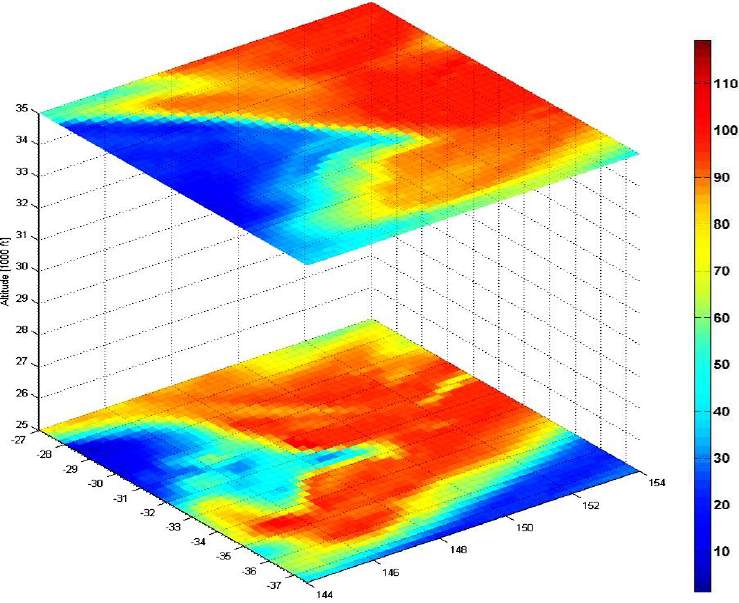
\includegraphics[width=\textwidth]{\FIGDIR/02_03_RelativeHumidity}
		\caption{Relative Humidity.} 
		\label{fig:humidityRelativeLocalizedExample}
	\end{subfigure}
	\vspace{1em} 
	\begin{subfigure}{0.45\textwidth} % width of right subfigure
		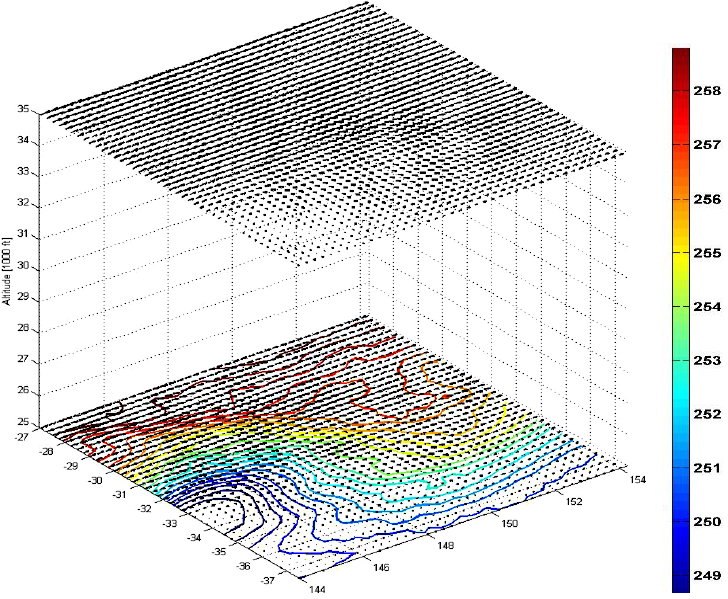
\includegraphics[width=\textwidth]{\FIGDIR/02_04_WindTemperature}
		\caption{Localized Wind Vectors.} % subcaption
		\label{fig:localizedWindVectorsExample}
	\end{subfigure}
	\caption{Localized Weather Model \cite{balaban2017dynamic}.} % caption for whole figure
	\label{fig:localizedWeatherModelExample}
\end{figure}
    
\paragraph{Localized Weather Impact Example:} An \emph{Icing Risk} in localized environment have been predicted based on numerical model \cite{thompson2017numerical}. It is shown that icing can be prevented by \emph{planned} and \emph{reactive} avoidance. The prevention can be done by placing hard or soft constraint into an environment. 

    
\paragraph{Weather Models:} \emph{Weather Models} can be extracted from \emph{Climate and weather model archive at the National Oceanic and Atmospheric Administration} \cite{rutledge2006nomads}. There is an example of troposphere winds (0 - 60 000 feet AMSL) (fig. \ref{fig:ExampleOfTroposphereWinds}) which can be useful in fuel efficient route planning. 
    
\begin{figure}[H]
    \centering
    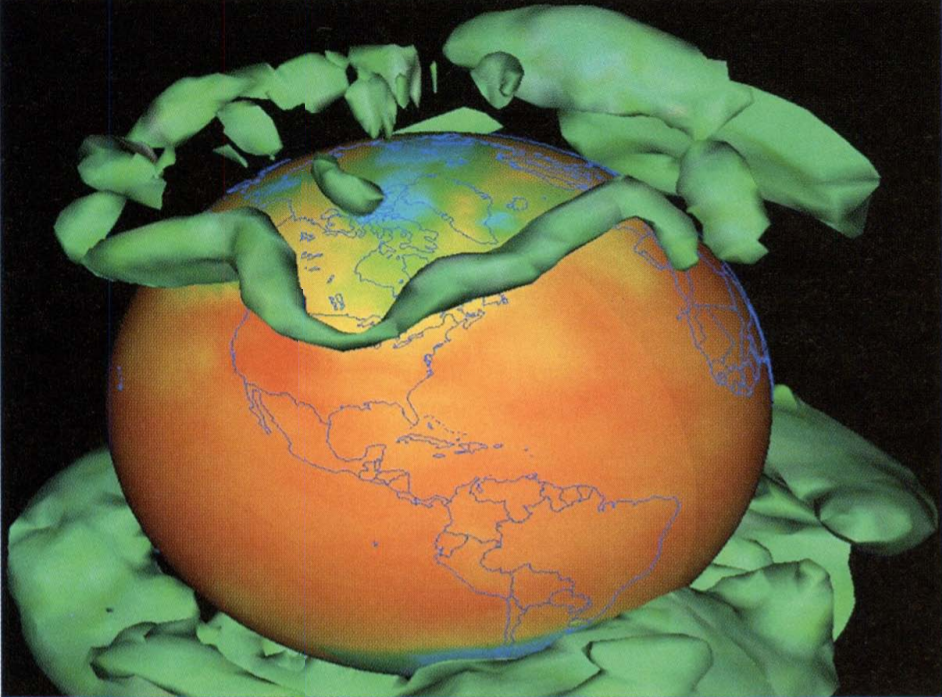
\includegraphics[width=0.7\textwidth]{\FIGDIR/02_01_IVS_Model}
    \caption{Example of upper troposphere winds \cite{rutledge2006nomads}.}
    \label{fig:ExampleOfTroposphereWinds}
\end{figure}
    %Functional decomposition removed
    %\section{(W) UTM Functional Decomposition}\label{sec:UTMFunctionaalDecomposition}
\begin{itemize}
    \item general thinking, approach 
    \item notification run
    \item resolution run
\end{itemize}

\subsection{(W) Information Exchange Principles}\label{sec:InformationExchangePrinciples}
\begin{itemize}
    \item Information Exchange schematics in general, describe data flow and actors
\end{itemize}

\subsubsection{ Collision Case}\label{sec:CollisionCase}
\begin{itemize}
    \item what collision case contains and how is calculated
    \item define conditions and role prioritization
    \item define blank spaces in VFR procedures 
\end{itemize}

\subsubsection{ Weather Case}\label{sec:WeatherCase}
\begin{itemize}
    \item This section needs to be discussed with subject matter expert.
\end{itemize}

\subsection{(W) Resolution Advisories}\label{sec:ResolutionAdvisiories}
\begin{itemize}
    \item just describe the resolution format from ATM
    \item discuss manned/unmanned interaction and reaction delays, reaction uncertainity, etc ...
\end{itemize}
\subsubsection{Movement Restriction}\label{sec:MovementRestriction}
\subsubsection{Convergence/Divergence}\label{sec:ConvergenceDivergence}

    
%03-Background theory
    \cleardoublepage
\chapter{Background Theory}\label{ch:backGroundTheory}

\paragraph{Motivation:} Cooperative and Non-Cooperative \emph{Sense and Avoid} (SAA) systems are key enablers for the \emph{Unmanned Aerial Systems} (UAS) to routinely access non-segregated airspace \cite{spriesterbach2013unmanned}. Both cooperative and non-cooperative SAA systems are being developed to address this integration requirement.

The \emph{DAA capability} is defined as the automatic detection of possible conflicts by the UAS platform under consideration and performing avoidance maneuvers to prevent the identified collisions. An analysis of the available DAA candidate technologies and the associated sensors for both cooperative and non-cooperative SAA systems is presented in \cite{muraru2011critical}. 

Non-cooperative \emph{Collision Detection and Resolution} (CD\&R) for UAS is considered as one of the major challenges that need to be addressed \cite{lai2012see} for the insertion of UAVs in non-segregated air space. As a result, many non-cooperative sensors for the SAA system have been adopted. Light Detection and Ranging (LIDAR)is used for detecting, warning and avoiding obstacles for low-level flying \cite{sabatini2014lidar}.

An approach to the definition of encounter models and their applications to SAA strategies is presented in \cite{kochenderfer2008encounter} for both cooperative and non-cooperative scenarios.

Since 2014, there is a visible strong political support for developing rules on drones, but regulations are harmonizing slowly. The European Aviation Safety Agency (EASA) has been tasked to develop a regulatory framework for drone operations and proposals for the regulation of "low-risk" UAS operations. In achieving this, EASA is working closely with the Joint Authorities for Regulation of Unmanned Systems (JARUS) \cite{jarus2016regulations}.

\paragraph{Background Areas:} Following Areas are introduced in this chapter:
\begin{enumerate}
    \item \emph{UAS System Model} (sec. \ref{s:uavMotionModel}) - continuous and discrete mathematical models.
    
    \item \emph{Reach Sets} (sec. \ref{s:ReachSets}) - introduction to representation and calculation methods.
    
    \item \emph{Hybrid Automaton} (sec. \ref{s:HybridAutomaton}) - intuitive definition  of the \emph{hybrid automaton}.
    
    \item \emph{LiDAR} (sec. \ref{sec:LiDARStateOfArt}) - a summary of \emph{LiDAR} technology and terminology introduction.
\end{enumerate}

    \section{(R) UAS System Model}\label{s:uavMotionModel}
\noindent
This section strongly follows \cite{lee2011structure}.

\subsection{Continuous-time systems}\noindent

\noindent Consider a class of systems given by functions:
\begin{equation}
    \begin{aligned}
    State Evolution &: input(time)  \to state(state_0,time) \\
    input(time)&: [0,FinalTime] \to \R^p \\
    input(time)&\in \mathbb{R}^p , state(t) \in \mathbb{R}^n \\
    \end{aligned}
\end{equation}
where $input(time)$ and $state(state_0,time)$ are a sets of continuous-time signals. These are often called continuous-time systems because they operate on continuous-time signals. 

Frequently, such systems can be defined by differential equations that relate the input signal to the output signal.

A prototypical description of a controlled (there is a control input signal) continuous-time system is:
\begin{multline}\label{eq:nonlinearsystem}
    \partial/\partial\text{t state}(time) =\\ f(time,state(time),input(time)), input(time) \in Inputs(time)
\end{multline}
where $f:\mathbb{R}\times\mathbb{R}^n\times\mathbb{R}^p\to\mathbb{R}^n$ satisfies the conditions for existence and uniqueness of the ordinary differential equation and $u$ is our control \cite{butcher1987numerical}.

\subsection{Discrete-time systems}
\noindent
\noindent Consider another class of systems given by functions
\begin{equation}\label{eq:Discretegenericuavmodel}
    \begin{aligned}
    State Evolution:& input(k)  \to state(k), \\
    k \in& \{0, t_s, 2.t_s, 3.t_s, \dots i.t_s\}, i \in \N^+\\
    input(k)\in& \mathbb{R}^p , state(k) \in \mathbb{R}^n\\
    \end{aligned}
\end{equation}
where $input(k)$, $state(k)$ is a set of discrete-time signals. They can be represented by a function $f$ like $f:\{0, t_s, 2.t_s, 3.t_s, \dots i.t_s\} \to \R^n,  i \in \N^+$ where $t_s$ is sampling time and $i$ is discrete step \cite{shampine1997matlab}.

\subsection{Adversarial behaviour in continuous systems}
\noindent Consider a subclass of continuous time systems where are two sets of control signals $uas(time)$ and $adversary(time)$ which are accommodated in following system:
\begin{equation}\label{eq:Adversarial}
    \begin{aligned}
    \partial / \partial \text{t state}(time)&= f(t,state(time),uas(time),adversary(time)), \\
    uas(time) &\in UAS Inputs(time) \subset \R^u, \\
    adversary(time) &\in Adversary Inputs(time) \subset \R^v \\
    \end{aligned}
\end{equation}
This system representation is often used in definition of problem of pursuit/evasion problem. Krasovskii developed a solution approach to this problem in \cite{game1987}. A complex example of can be found in article \cite{game1988}.
    \section{Reach Sets}\label{s:ReachSets}
    \noindent Informally, the \emph{Reach Set} of a UAS system described by a differential equation is the \emph{set of all states that can be reached from an initial state within a given time interval}.

\subsection{Definitions}\label{sec:reachSetIncrementalDefinition}
    \paragraph{For following definitions} consider \emph{nonlinear UAS system} described in (sec. \ref{s:uavMotionModel}).
    
    \begin{definition}[Reach set starting at a given point]\label{def:reachset01}
        Suppose the initial position
        and time $(state_0, time_0)$ are given. The reach set $ReachSet[\tau, time_0, state_0]$ of \emph{nonlinear system} at time $\tau \ge time_0$, starting at $(state_0, time_0)$ is given by:
        \begin{equation}
            ReachSet[\tau, time_0, state_0] = \bigcup \{state(\tau):input(s)\in Inputs(s),s \in (time_0,\tau]\}
        \end{equation}
    \end{definition}
    
    \paragraph{Reach set starting at given set} can be used to determine reach set in case of \emph{hybrid system} input control switch and it is defined as follow:
    \begin{definition}\label{def:ReachSetBasic} set starting at a given set]
        The reach set at time $\tau > t_0$ starting from set $States_0$ is defined as:
        \begin{equation}
            ReachSet[\tau, time_0, States_0] = \bigcup \{ReachSet[\tau, time_0, state_0]: state_0 \in States_0\}
        \end{equation}
    \end{definition}

    \paragraph{Reach set for adversarial behavior} can be used to calculate possible escape routes from pursuer and it is defined as follow:

    \begin{definition}[Reach set under adversarial behavior]
        Consider now the case of adversarial behavior(\cite{game1987,game1988}).
        where $input(t)$ is our control and $adversary(t)$ is adversary control which is independent of $input(t)$, let $differentialControl(t)=input(t)-$ $\sup_{{state} \in state(t)}$\\ $adversary(t)$, which represents worst possible input change in given state and time, then \emph{reach set for system} is represented as:
        \begin{equation}
            ReachSet\left[\begin{gathered}\tau,\\ time_0,\\ state_0\end{gathered}\right] = \bigcup \left\{state(\tau): 
                \begin{aligned}
                    differentialControl(s)\in\\  DifferentialControlSet(s)
                \end{aligned}
            ,s \in (time_0,\tau]\right\}
        \end{equation}
    \end{definition}

    \paragraph{Reach set under constraints} are usable to define state constrained systems in terms of dynamics and technical capabilities.
    
    \begin{definition}[Reach set under state constraints]
        Suppose the initial position and time $(state_0, time_0)$ and $state$ constraints are given $state(t) \in \mathbb{A} \subset \R^n, \dot{x}(t) \in \mathbb{B} \subset \R^n$. The reach set $ReachSet[\tau, time_0, \vec{state}_0]$ of \emph{nonlinear UAS system} at time $\tau \ge time_0$, starting at position and time $(state_0, time_0)$ is given by:
        
        \begin{equation}
            ReachSet\left[\begin{gathered}\tau,\\ time_0,\\ state_0\end{gathered}\right] = \bigcup 
            \left\{
                state(\tau):
                \begin{gathered}
                    \forall s\in (time_0,\tau], state(s) \in \mathbb{A},\\ 
                    \dot{state}(s) \in \mathbb{B},\\ 
                    \exists input(s) \in Inputs(s)
                \end{gathered}
            \right\}
        \end{equation}
        
    \end{definition}


    \subsection{Computation of Reach Sets}
    \noindent   Several techniques for reachability analysis of systems have been proposed. They can be (roughly) classified into two kinds:
    
    \begin{enumerate}
    \item Purely symbolic methods based on: 
        \begin{enumerate}[a.]
        \item the existence of analytic solutions of the differential equations and 
    
        \item the representation of the state space in a decidable theory of the real numbers.
        \end{enumerate}
    \item Methods that combine 
    \begin{enumerate}[a.]
        \item numeric integration of the differential equations
    
        \item symbolic representations of approximations of state space typically using (unions of) polyhedra or ellipsoids.
        \end{enumerate}
    \end{enumerate}
    These techniques provide the algorithmic foundations for the tools that are available for computer-aided verification of hybrid systems (\cite{daws1996tool}, \cite{henzinger1994symbolic}, \cite{henzinger1995hytech}).

    The set-valued Lebesgue integral provides a conceptual tool for the direct computation of the reach set. In what follows we describe techniques from dynamic optimization which are used to compute reach sets for dynamic systems.

    The relation between dynamic optimization and reachability was first observed in \cite{leitmann1982optimality}. A typical problem of optimal control can be formulated as follows:

    \begin{equation}
        \max \left(
        \begin{gathered}
            \int_{initialTime}^{finalTime} cost(time,state(time),contro(time)) \textnormal{d}time + \dots \\ \dots +FinalCost(state(finalTime))\end{gathered}
        \right)
    \end{equation}
    
    \noindent For nonlinear system:
    \begin{equation}
        \dot{state}(t) = f(t,state(t),control(t)), control(t) \in ControlSet(t) \subset \R^p
    \end{equation}
    
    Where $cost$ is given as cost function of time,state and input and $FinalCost$ represents cost functional.
    There are two main techniques to solve this problem: 
    
    \begin{enumerate}
        \item The maximum principle
        
        \item Dynamic programming. The maximum principle gives necessary conditions of optimality. Dynamic programming may be used to derive sufficientconditions of optimality.
    \end{enumerate}

    A good reference on the maximum principle is \cite{pontryagin1962ef}. A less known reference with detailed geometric interpretations is \cite{girsanov2012lectures}. A good reference on dynamic programming is \cite{bardi2008optimal}.
    
    %\section{(W) Space Segmentation}\label{s:spaceSegmentation}
    \emph{To be done here:}
    \begin{itemize}
        \item Polar space segmentation.
        \item local vs global space segmentation.
        \item benefits of uneven space segmentation.
    \end{itemize}
    \newpage
\section{(R) Movement Automaton}\label{sec:MovementAutomatonBackground}

    \noindent\emph{Movement Automaton} is basic interface approach for discretization of \emph{trajectory evolution}  or \emph{control input} for any \emph{continuous or discrete system model}.
    
    \emph{Main function} of \emph{Movement Automaton is} for system given by equation $\dot{state}=f(time,state,input)$ with initial state $state_0$ to generate \emph{reference trajectory} $\hat{state}(t)$ or \emph{control signal} $input(t)$.
    
    Using \emph{Movement Automaton} as \emph{Control Proxy} will provide us with \emph{discrete command chain} interface. This will reduce the \emph{non deterministic} element from \emph{Evasive trajectory} generation, by reducing infinite maneuver set to finite \emph{movement set}.
    
    \emph{Non determinism} of \emph{Avoidance Maneuver} have been discussed as an issue in following works:
    \begin{enumerate}
        \item Newton gradient method for evasive car maneuvers \cite{vsantin2011combined}.
        \item Non-holistic methods for trajectory generation \cite{pin1990autonomous}.
        \item Stochastic approach to elliptic trajectories generation \cite{andrzejak2001epileptic}.
    \end{enumerate}
    
    \emph{Examples} of \emph{Movement Automaton Implementation} as \emph{Control Element} can be mentioned as follows:
    \begin{enumerate}
        \item Control of traffic flow \cite{kuwata2009real}.
        \item Complex air traffic collision situation resolution system  \cite{frazzoli2001robust,frazzoli2000trajectory}.
        \item SAA/DAA capable avoidance system \cite{gomola2017obstacle}.
    \end{enumerate}


    \subsection{Hybrid Automaton}\label{s:HybridAutomaton}
    \noindent First the notion of  \emph{hybrid} automaton  \cite{lazar2006model,borrelli2006mpc,daws1996tool} needs to be introduced:

    \begin{definition}{Hybrid automaton} (\ref{eq:hybridAutomaton}) is given as structure:
        \begin{equation}\label{eq:hybridAutomaton}
        \begin{aligned}
            HybridAutomaton(&States,SystemState,VectorField,\\
                            &DiscreteTransition,ResetMap)
        \end{aligned}
        \end{equation}
    
        \emph{States} ($Q$) is given as set of discrete states, for every time $t\in Domain$ hybrid automaton stays in exactly one of \emph{states}.
    
        \emph{SystemState} ($x$), is given in domain $x\in\R^n,n\in\N^+$, representing the trajectory evolution.
        
        \emph{VectorField} ($f$) (\ref{eq:vectorField}) is bounded to single $State\in States$ and represents local SystemState evolution, when given automaton State is Active.
        
        \begin{equation}\label{eq:vectorField}
            VectorField: State\times SystemState \to SystemState
        \end{equation}
        
        \emph{DiscreteTransition} ($\varphi$) (eq. \ref{eq:discreteTransition}) indicates changes of states in automaton, the changes are triggered by satisfying specific condition given by State and SystemState. 
        
        \begin{equation}\label{eq:discreteTransition}
            DiscreteTransition:State\times SystemState \to State
        \end{equation}
        
        \emph{ResetMap} ($\rho$) (eq. \ref{eq:resetMap}) defines changes of State to some default value, this change is triggered by specific automaton State and SystemState.
        
        \begin{equation}\label{eq:resetMap}
            ResetMap:State\times SystemState \to SystemState
        \end{equation}
    
    \end{definition}

\subsection{Building Blocks}\label{s:MovementAutomatonBuidlingBlocks}
    \begin{definition}{Movement Primitive:}\label{def:MovementPrimitive}\\\emph{States} from \emph{Hybrid automaton} can be taken as \emph{Movements} in \emph{Movement Automaton}. \emph{MovementPrimitive} (eq. \ref{eq:movementPrimitive}) is describing the \emph{Movement} behaviour as transfer function \emph{VectorField} enriched with parameters. 

    \begin{equation}\label{eq:movementPrimitive}
        \begin{aligned}
            &MovementPrimitive(vectorField,minimalDuration,parameters)\\
            &VectorField:SystemState\times parameters \to SystemState
        \end{aligned}
    \end{equation}
    \end{definition}



    \paragraph{Example: }Let say that \emph{UAS} system is given as $\dot{position}=velocity$, then let us have two \emph{MovementPrimitives}:
    
    \begin{enumerate}
        \item \textit{Stay} - $minimalTime=1s$, $parameters=\{\}$, $VectorField:\dot{position}=0$.
        \item \textit{Move} - $minimalTime=1s$, $parameters=\{velocity\}$, $VectorField:\dot{position}=velocity$.
    \end{enumerate}
    
    \paragraph{Trajectory from Movement Primitives:} The \emph{UAS} should \emph{Move} for $5s$ with velocity $10 m/s$, then \emph{Stay} for $10s$, then move for $7s$ with velocity $4 m/s$, with initial position $position_0=0$ and initial time $t_0=1$ The standard approach is to derive transfer function $position = \Theta(\dots)$
    \begin{equation}\label{eq:trajectoryExample}
        position(t)=\Theta(\dots)
        \begin{cases}
            t \in [0,5] &: 10\times t + position(0)\\
            t \in (5,15] &: 0\times (t-5) + position(5)\\
            t \in (15,22]&: 4\times (t-15) + position(15)
        \end{cases}
    \end{equation}

    The \emph{example} given by (eq. \ref{eq:trajectoryExample}) is fairly primitive, but imagine UAS system given by nonlinear dynamics $\dot{x}=f(x,u,t)$ \cite{fossen2011mathematical}. Then defining transfer function for given command chain can be impossible.

    \begin{definition}{Movement Transition:}\label{def:movementTransition}\\
        \emph{System state} can be different than intended movement application, the notion of \emph{Transition} is therefore introduced as stabilizing element in movement chaining (eq. \ref{eq:movementTransition}).
        \begin{equation}\label{eq:movementTransition}
            Transition:MovementPrimitive\times SystemState \to MovementPrimitive    
        \end{equation}
    \end{definition}

    \paragraph{Trajectory with Transitions:} Introducing two transitions $Transition(Move,Stay)$ and $Transition(Stay,Move)$ reflecting periods when vehicle stop moving or speed-up to desired velocity. The transfer function (eq. \ref{eq:trajectoryExample}) can be rewritten as combination of \emph{MovementPrimitives} (eq. \ref{eq:movementPrimitive}) and \emph{Transitions} (eq. \ref{eq:movementTransition}):
    
    \begin{multline}
        Transition(Stay,Move), Move(5s,10m/s),\\
        Transition(Move,Stay), Stay(10s),\\ 
        Transition(Stay,Move), Move(7s,4m/s)
    \end{multline}.

    \begin{note} There are two types of \emph{MovementPrimitives}:
    \begin{enumerate}
        \item \emph{Stationary} - when system state is considered neutral and they are considered as entry point for automaton.
        \item \emph{Dynamic} - when the system state is considered evolving and they needs to be terminated with \emph{stationary} transition.
    \end{enumerate}
    \end{note}

    \paragraph{Movement Mapping Example:} Transition/MovementPrimitive pairs (eq. \ref{eq:movementTransition}) can be mapped into movements (eq. \ref{eq:movementMappingExample}).
    
    \begin{equation}\label{eq:movementMappingExample}
    \begin{aligned}
        Move(5s,10m/s) &:Transition(Stay,Move), Move(5s,10m/s),\\
        Stay(10s) &: Transition(Move,Stay), Stay(10s),\\ 
        Move(7s,4m/s) &: Transition(Stay,Move), Move(7s,4m/s)
    \end{aligned}    
    \end{equation}

    \begin{definition}{Movement:}\label{def:Movement}\\
        Movement can consist from multiple \emph{Transitions} (eq. \ref{eq:movementTransition}) and one \emph{MovementPrimitive} (eq. \ref{eq:movementPrimitive}), the duration of \emph{MovementPrimitive} can be shortened by \emph{Transitions} duration. \emph{Movement} is defined as follows:
        
        \begin{equation}
            \small Movement \left(
                \begin{gathered}
                    \scriptstyle initialState,\\
                    \scriptstyle initialTime[0..1],\\ 
                    \scriptstyle duration,\\ 
                    \scriptstyle parameters[0..1]
                \end{gathered}\right)
            = \small Chain \left(
            \begin{gathered}
            \small InitialTransition(\dots)[0..*],\\
            \small MovementPrimitive\left(
            \begin{gathered}
                \scriptstyle transitionState,\\
                \scriptstyle remainingDuration,\\
                \scriptstyle parameters
            \end{gathered}\right)\\
            \small LeaveTransition(\dots)[0..*],\\
            \end{gathered}
            \right)
        \end{equation}
        
        \emph{Chain function} connects multiple \emph{initial Transitions} which are appliead at \emph{initialState} at \emph{initialTime}. Then own \emph{MovementPrimitive} (eq. \ref{eq:movementPrimitive}) is invoked with \emph{transitionnsState}. \emph{Transitions state} is state changed by \emph{Initial Transitions}. After \emph{Movement Primitive} there can be \emph{Leave Transitions Movement}
    \end{definition}

    \paragraph{Minimal Movement Time:} Given by (eq. \ref{eq:minimalMovementTime}) for \emph{movement} is given as sum of \emph{MovementPrimitive} (eq. \ref{eq:movementPrimitive}) minimal time, and \emph{Transition} (eq. \ref{eq:movementTransition}) in/out combined minimal time.
    
    \begin{equation}\label{eq:minimalMovementTime}
        minimalTime(Movement)=
        \begin{aligned}
        &minimalTime(MovementPrimitive) +\\ &\text{max}_{in/out}\left\{time(Transition)\right\}
        \end{aligned}
    \end{equation}

	\newpage    
    \paragraph{Movement Chaining:}\emph{Movements} can be \emph{chained} and applied to initial \emph{system state} to generate \emph{system trajectory}. Example of trajectory is given by (eq. \ref{eq:trajectoryExample}). Movements are reversibly obtained by participation such \emph{trajectory} into \emph{Movement primitives} and \emph{Transitions}. Then sample \emph{Trajectory} for $n\in \N^+$ movements looks like (eq. \ref{eq:movementChaining}).
    \begin{equation}\label{eq:movementChaining}
        \begin{aligned}
        &Trajectory(t_0)=State(t_0)\\
        &Trajectory(t_0,t_1]=Movement_1(Trajectory(t_0),t_0,duration_1,parameters_1)\\
        &Trajectory(t_1,t_2]=Movement_2(Trajectory(t_1),t_1,duration_2,parameters_2)\\
        &Trajectory(t_2,t_3]=Movement_3(Trajectory(t_2),t_2,duration_3,parameters_3)\\
        &\vdots\\
        &Trajectory(t_{n-1},t_n]=Movement_n(Trajectory(t_{n-1}),t_{n-1},duration_n,parameters_n)\\
        \end{aligned}
    \end{equation}

    Given \emph{Trajectory} at time $t_0$ is given as initial \emph{State} of \emph{System}. For time interval $(t_0,t_1)$, which length is equal to $duration_1$, the \emph{State} is given by $Movement_1$ with $parameters_1$ and base time $t_0$. This behaviour continues for movements $2,\dots,n$. 

    \begin{definition}{Movement Buffer:}\label{def:MovementBuffer}\\
        \noindent\emph{Movements} can be chained into \emph{Buffer} with assumption of \emph{continuous movement execution}. \emph{Continuous movement executions} each movement in chain (eq. \ref{eq:movementChaining}) is executed in time interval $\tau_i=(t_{i-1},t_{i}]$ where $i$ is movement order and $\forall$ $Movement_i$ starting time is $t_0$ or $t_{i-1}$ from previous movement. With given assumption \emph{Buffer} is given as (eq. \ref{eq:movementBuffer}) with parameters $t_{i-1},t_{i}$ omitted, due $t_0$ and $duration_i$ dependency.
        
        \begin{equation}\label{eq:movementBuffer}
            Buffer = \left\{Movement_i(duration_i,parameters_i)\right\}i\in\N^+
        \end{equation}
    \end{definition}
    
    \begin{definition}{Movement Automaton Trajectory:}\label{def:MovementAutomatonTrajectory}\\
        Let say system \emph{State}$\in\R^n$ which \emph{Trajectory} is defined by movement chaining (eq. \ref{eq:movementChaining}), applied on some \emph{initial time} $t_0\in\R^+$ and final time $t_f=t_0+\sum_{i=1}^{I}duration_i$, with movements contained in \emph{Buffer} (eq. \ref{eq:movementBuffer}) is given as \emph{Trajectory} (eq. \ref{eq:TrajectoryDefinition}).
        
        \begin{equation}\label{eq:TrajectoryDefinition}
            Trajectory(t_0,State(t_0),Buffer)\text{ or } Trajectory(State_0,Buffer) \text{ if } t_0=0
        \end{equation}
    \end{definition}


    \begin{note}
        The space dimension of \emph{Trajectories} is $\R^{n+1}$ if the space dimension of state \emph{Space} is $R^n$, because \emph{Trajectory space} contains evolution of \emph{Space} in time interval $T[t_0,t_f]$.
        
        The transformation from \emph{transfer function} (eq. \ref{eq:trajectoryExample}) to \emph{trajectory} (eq. \ref{eq:TrajectoryDefinition}) is natural, only set of \emph{Movement primitives} (eq. \ref{eq:movementPrimitive}) and set of \emph{Transitions} (eq. \ref{eq:movementTransition}) is required.
    \end{note}

    \paragraph{State Projection:} \emph{Trajectory} (eq. \ref{eq:TrajectoryDefinition})is naturally evolution of space over time, then there exists \emph{StateProjection} function (eq. \ref{eq:stateprojection}) which returns \emph{State} for specific \emph{Time}.
    
    \begin{equation}\label{eq:stateprojection}
        StateProjection:Trajectory\times Time \to State(Time)
    \end{equation}

\newpage    
\subsection{Definition}\label{s:MovementAutomatonDefinitionAndProperties}

    \begin{definition}\label{def:movementAutomaton}Movement Automaton is given as follow:
    
    \begin{align}   
        \label{eq:madInitialState}
        InitialState&: \in \R^h, h\in \N^+\\
        \label{eq:madSystemdefinition}
        System&: \dot{State}=f(Time,State,Input)\text{ or } vectorField\\
        \label{eq:madMovementPrimitive}
        Primitives &= \left\{MovementPrimitive_i\left(
                                \begin{aligned}
                                &vectorField,\\
                                &minimalDuration,\\
                                &parameters
                                \end{aligned}\right)
                            \right\} i \in \N^+\\
        \label{eq:madTransitions}
        Transitions&= \left\{Transition_j\left(
                                \begin{aligned}
                                    &MovementPrimitive_l,\\
                                    &MovementPrimitive_k
                                \end{aligned}\right)_{k\neq l}\right\} j\in N^+\\
        \label{eq:madMovements}
        Movements&= \left\{Movement_m\left[
                                \begin{aligned}
                                    &Transition_o[0..*],\\
                                    &MovementPrimitive_p\\
                                    &Transition_r[0..*],\\
                                \end{aligned}\right]_{o \neq r}\right\}  m\in N^+\\
        \label{eq:madBuffer}
        Buffer&= \left\{Movement_s(duration_s,parameters_s)\right\} s\in \N^+\\
        \label{eq:madExecuted}
        Executed&= \left\{Movement_s(duration_s,parameters_t)\right\} t\in \N^+\\
        \label{eq:madBuilder}
        Builder&:Movement \times MovementPrimitive \to Movement\\
        \label{eq:madTrajectory}
        Trajectory&:InitialState\times Movement^u \to State \times Time, u\in N^+\\
        \label{eq:madStateProjection}
        StateProjection&:Trajectory\times Time \to State(Time)  
    \end{align}
    
    \noindent \emph{System} (eq. \ref{eq:madSystemdefinition}) is given in form of \emph{differential equations} $\dot{x} = f(t,x,u)$ or \emph{other transformable equivalent}, with \emph{initial state} (eq. \ref{eq:madInitialState}).
    
    \emph{Movements} (eq. \ref{eq:movementChaining}) are defined as sequence of necessary \emph{initial transitions} (eq. \ref{eq:madTransitions}), \emph{movement primitive} (eq. \ref{eq:madMovementPrimitive}), and, \emph{leave transitions} (\ref{eq:madTransitions}).
    
    \emph{Buffer} contains a set of \emph{movement primitives} (eq. \ref{eq:madMovementPrimitive}) to be executed in order to achieve desired goal. \emph{Builder} (eq. \ref{eq:madBuilder}) assures that first \emph{movement primitive} (eq. \ref{eq:movementPrimitive})from \emph{Buffer} (eq. \ref{eq:madBuffer}) is transformed into \emph{next movement} (eq. \ref{eq:madMovements}) based on \emph{current movement} (eq.\ref{eq:madMovements}).
    
    System \emph{trajectory} (eq. \ref{eq:madTrajectory}) is defined in (eq. \ref{eq:TrajectoryDefinition}). \emph{State projection} (eqs. \ref{eq:stateprojection},\ref{eq:madStateProjection}) is giving \emph{State} variable for time $t\in[t_0,t_{max}]$ where $t_max$ is given by:
    \begin{equation}
    t_{max}=t_0+\sum_{i=1,u}Buffer.Movement(i).movementDuration    
    \end{equation}
    \end{definition}
    
    \begin{note}{From Continuous Reach set to Movement Automaton Control Reach Set:}\label{eq:fromContRStoMARS}

\emph{The reach set $R$} (\ref{eq:reachSetExample1}) for system $\partial/\partial \text{t state} =model(state,input)$ with initial state $state_0=state(t_i)$ in time interval $[t_i,t_{i+1}[$  is with existing control strategy $input(t)\in Control Strategy(t)$. The reach set $R(state_0, t_0,t_1)$ where $t_1 > t_0$.
\begin{equation}\label{eq:reachSetExample1}
    R(state_0, t_0,t_1) = \bigcup \left\{state(s):input(s)\in Control Strategy(s), s\in (t_0,t_1]\right\} 
\end{equation}


\noindent\emph{The reach set $\mathscr{R}$} (\ref{eq:reachSetExample2}) of the system under the control of the \emph{movement automation} consist from the set of trajectories $Trajectory(initialState,buffer)$, which are executed in constrained time period $[t_i,t_{i+1}[$.
\begin{multline}\label{eq:reachSetExample2}
     ReachSet(state_0,t_i,t_{i+1})=\\\left\{Trajectory(state_0,buffer):\text{duration}(buffer) \le (t_{i+1}-t_i)\right\}
\end{multline}
\end{note}

\begin{note}{Weak Invariance:}

When the UAS is under the control of the movement automaton  for the obstacle avoidance problem,  by design of the avoidance algorithm, the trajectories of the UAV will not intersect any threat. This means that the controlled system $\partial/\partial \text{t state} =model(state,input)$ is \emph{weakly invariant} with respect to the complement of the threats, and with respect to the free space. A pair $(state, SafeSpace)$, where $\partial/\partial \text{t state} =model(state,input)$ and $SafeSpace$ is a closed set, is weakly invariant if there exist controls such that a trajectory starting inside $State_0\in SafeSpace$ remains inside $State (t)\in SafeSpace$ \cite{blanchini1999set}.
 \end{note}
    \section{(R) LiDAR}\label{sec:LiDARStateOfArt}
\noindent \paragraph{LiDAR(Light Detection And Ranging)} is active form of remote sensing: information is obtained from a signal which is sent from a transmitter and reflected by a target, and detected by a receiver back at the source. Following types of information can be obtained:
\begin{enumerate}
\item \textit{Range to target} - topographic LiDAR or laser altimeter.
\item \textit{Chemical properties of target} - differential absorption LiDAR.
\item \textit{Velocity of target} - Doppler LiDAR.
\end{enumerate}

\noindent Chemical properties of target are out of scope. Velocity of  target seems as interesting property to investigate, but this type of LiDAR is usually used for meteorological measurements of wind currents \cite{martin2011meteorological}. Extended research in LiDAR as obstacle detection sensor has been executed by research group around Sabatini \cite{sabatini2014lidar} and Ramasy \cite{ramasamy2016lidar}. 

LiDAR output is represented as point cloud it is described by following definition.
\begin{definition}[Scanned point and Point-cloud]
Consider viewpoint as origin of $\R^3$ space,  Let  $point \in Planar Coordinates$ be defined as:
    \begin{equation}
        point = [ distance, horizontal^\circ, vertical^\circ, time ]^T
    \end{equation}
    Where $horizontal^\circ$ is horizontal angle from origin, $vertical^\circ$ is vertical angle to origin, and, $time$ is time of retrieval.\\

    \noindent Point-cloud is set of points scanned in small enough time-frame, based on processing raw point data it can have following representations:
    
    \begin{enumerate}
        \item Local point-cloud - position of sensor is used as origin of space and points can be represented in orthogonal or planar representation. 
        
        \item Global point-cloud -global position of sensor is used as reference to calculate global position of points.
    \end{enumerate}
\end{definition}

\paragraph{Point-cloud} is usually addressed as \textit{raw point-cloud} in case if its represented in Local planar coordinates. Other forms of point cloud require further processing and they are not feasible for real-time obstacle detection and avoidance \cite{chen2007airborne}.

\begin{figure}[H]
    
    \begin{subfigure}{0.5\textwidth}
        \centering
        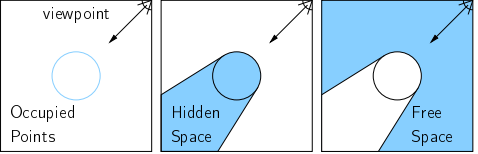
\includegraphics[width=0.9\linewidth]{\FIGDIR/10_Lidar_sets1.PNG} 
        \caption{Space type definitions}
        \label{fig:Spacetypes}
    \end{subfigure}
    \begin{subfigure}{0.5\textwidth}
        \centering
        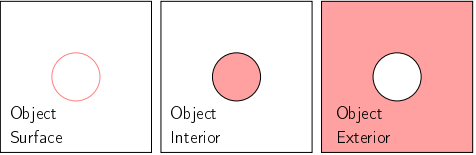
\includegraphics[width=0.9\linewidth]{\FIGDIR/11_Lidar_sets2.PNG}
        \caption{Object properties definitions}
        \label{fig:ObectProperties}
    \end{subfigure}
    
    \caption{Six space classifications \cite{yapo2008probabilistic}.}
    \label{fig:Spaces of interests}
 \end{figure}
 
\noindent  Because of real-time obstacle avoidance it is necessary to introduce following terminology:
\begin{enumerate}
    \item \textit{Occupied points} - points which have been detected by LiDAR (also addressed as visible points).
    \item \textit{Hidden space} - space which is hidden behind occupied points, from viewpoint it is uncertain what is in that space. 
    \item \textit{Free space} - space which is visible from viewpoint and it is not occupied by known objects.
    \item \textit{Object surface} - detected and undetected object surface
    \item \textit{Object interior} - occupied space by object.
    \item \textit{Object exterior} - free space around known objects.
\end{enumerate}

\noindent Existing method for space segregation \cite{yapo2008probabilistic} leads to following definition:

\begin{definition}[Accessible space]\label{def:accessibleSpace}
    Consider known space as space explored by sensor (it can have different viewpoint along previous 3D trajectory).
    Intersection between \textit{object exterior} ($Exterior$) and \textit{free space} $Free$ gives us \textit{Accessible space} ($Accessible$).
    \begin{equation}
        Accessible = Exterior(object) \cap Free(object)
    \end{equation}
\end{definition}
 
 \noindent Accessible space $S_A$ (def. \ref{def:accessibleSpace}) is our bordering limitation for reachable space of system $ReachSet[\tau, time_0, state_0]$ (def. \ref{def:reachset01}.).

%04-Problem Statement
    %%\chapter{Problem Statement}


\section{Basic Definitions}\label{s:basicDefinitions}
    \begin{definition}{\emph{Obstacle} $o$} is given as any inaccessible set of points $o\subset\R^3$ it can be represented as polygon, space boundary, thick point-cloud, separation plane.
    \end{definition}
    
    \begin{definition}{Information source $s$}\label{def:informationSource} is source of obstacle information to relative vehicle position and orientation $\vec{p}\in\R^6$ with time $t$ mapping capability. The information source can be sensory reading, obstacle map,weather forecast zones, and, \emph{Air Traffic Management} restrictions.
    
    Information sources are aggregated in \emph{information source set} $\mathscr{S}$.
    
    \emph{Information source} $s\in\mathscr{S}$ provides \emph{obstacle feed} $\mathscr{O}_s$ depending on vehicle position and orientation $\vec{p}$ and time $t$. Overall obstacle set is aggregation of obstacle feeds from \emph{information source set}
    \begin{equation}\label{eq:obstacleSet}
        \mathscr{O}(\vec{p},t)=\bigcup_{s\in\mathscr{S}} \mathscr{O}_s(\vec{p},t), \quad \mathscr{O}_s(\vec{p},t)=s(\vec{p},t)
    \end{equation}
    \end{definition}
    
    \begin{definition}{\emph{Field of vision}}\label{def:} (FOV) of vehicle or sensor is given as subset $\mathscr{F}\subset\R^3$ with position and orientation $\vec{p}\in\R^6$, for time $t$. Field of the vision is denoted $\mathscr{F}(\vec{p},t,s)$, where $s\in\mathscr{S}$ is sensor from sensory field, or $\mathscr{F}(t)$, in case $\vec{p}$ is implicit from vehicle position $\vec{p}=\vec{x}(t)\to\R^6$ and sensor is implicit.
    \end{definition}
    
    \begin{note} Field of the vision for vehicle is combination of all field of the visions from information sources $\mathscr{S}$:
    \begin{equation}\label{eq:fieldOfVisonFixedTime}
        \mathscr{F}(t)=\bigcap_{s\in\mathscr{S}} \mathscr{F}(\vec{p},t,s)
    \end{equation}
    \end{note}
    
    \begin{definition}{Space segmentation}\label{def:spaceSegmentation} of any space $\mathscr{A}=\R^k, k\in\N^+$ is given as separation of space to exclusive sets $c_\mathbb{I}\subset\mathscr{A}$ called cells, with index vector $\mathbb{I}\subset\mathbb{Z}^l$ serving as unique identifier.The segmentation holds following properties:
    \begin{enumerate}
        \item Cells are covering segmented space $\bigcup_{\forall i\in \mathbb{I}\subset\mathbb{Z}^l} c_i = \mathscr{A}$
        \item Each cell $c_\mathbb{I}\in\mathscr{A}$ is nonempty set.
        \item Each point $\vec{p}\in\R^k$ in one cell $\vec{p}\in c_i$ shares same property value $P(\vec{p},\dots)$ with any point $\vec{r}\neq\vec{p}$ 
    \end{enumerate}
    
    \end{definition}
    
    \begin{definition}{Obstacle space $\mathscr{O}$} is segmentation (def. \ref{def:spaceSegmentation}) of obstacle set $\mathscr{O}(\vec{p},t)$ (\ref{eq:obstacleSet}).
    \end{definition}
    
    \begin{definition}{Free space $\mathscr{F}$} is space where exists direct visibility between observation point $\vec{p}\in\R^m$ and points in segmented space (def. \ref{def:spaceSegmentation}).
    \end{definition}
    
    \begin{definition}{Uncertain space $\mathscr{U}$} contains space segments (def. \ref{def:spaceSegmentation}) which are not in obstacle or free space.
    \begin{equation}
        \mathscr{U}=(\mathscr{A}-\mathscr{F})-\mathscr{O}
    \end{equation}
    \end{definition}
    
    \begin{definition}{\emph{Intruder}(moving obstacle) $i$} is identified via information source $s\in\mathscr{S}$ with minimal set of properties bounded to time of detection $t$:
    \begin{enumerate}
        \item position $\vec{p}\in\R^k$,
        \item velocity $\vec{v}\in\R^k$,
        \item intruder body radius (vehicle class) $r\in\R^+$,
        \item uncertainty spread $\Theta\in\R^{k-1}$.
    \end{enumerate}
    
    \end{definition}

\section{Avoidance set}\label{s:AvoidanceSet}
    \begin{definition}{Avoidance set $\mathscr{A}(t,\vec{x}_0,\vec{u}_0,\mathscr{S})$} is defined for vehicle system:
    \begin{equation}
        \dot{\vec{x}}(t)=\vec{f}(t,\vec{x},\vec{u})
    \end{equation}
    With system state $\vec{x}(t)\in\R^n$, control signal $\vec{u}(t)\in\R^k$. Regardless of system class the system entry point is given as $\vec{e}$:
    \begin{equation}
        \vec{e}= [\vec{x}_0,\vec{u}_0,t_0,d_0]\in\R^{n+k+1+1}
    \end{equation}
    Initial state $x_0$ at time $t_0$ is accompanied with initial input signal $u(t)$, initial time $t_0$, and initial decision $d_0\in\N$. Note that structure can store multiple system trajectories due the discrete decision dimension $d\in\N$.
    
    For time period $\tau\in[t_0,t]$ vehicle fly along the trajectory $\vec{x}(\tau)$ based on taken decisions $D=\{d_0,d_1,\dots,d_i\},i\in\N$ in decision times $T_D=\{t_{d1},t_{d2},\dots,t_{di}\}, t_{di}\le t$. Field of the vision $\mathscr{F}(\tau)$ along trajectory $\vec{x}(\tau)$ is given as:
    \begin{equation}
        \mathscr{F}(\tau) = \bigcup_{t_d\in T_D} \mathscr{F}(\vec{x}(t_d)\to\vec{p},t_d,\forall s\in\mathscr{S}) \quad (\ref{eq:fieldOfVisonFixedTime})
    \end{equation}
    \end{definition}
    Aggregated field of the vision $\mathscr{F}(\tau)$ is separated into obstacle space $\mathscr{O}(\tau)$ uncertain space $\mathscr{U}(\tau)$ and free space $\mathscr{F}(\tau)$. Then for any fixed time $t_{fix}\in[t_0,\infty)$ all system trajectories $x(t)$ starting within entry point $\vec{e}$ holds following conditions:
    \begin{enumerate}
        \item Each projected point $\vec{p}=\vec{x}(t_{fix})\to\mathscr{F}(\tau)$ belongs to free space $\mathscr{F}(\tau)$.
        \item Each projected point $\vec{p}$ has minimal distance from obstacle space $\mathscr{O}(t_{fix})$ or $\mathscr{U}(t_{fix})$ greater than safety margin $s_m$.
    \end{enumerate}
    
    \begin{note} Note following attributes of avoidance set ($\mathscr{A}(t,\vec{x}_0,\vec{u}_0,\mathscr{S})$):
    \begin{enumerate}
        \item \emph{Avoidance set respects vehicle dynamics} - avoidance set contains trajectories which are feasible for vehicle dynamics and control.
        \item \emph{Avoidance set stores multiple system trajectories} due the added decision dimension.
        \item \emph{Avoidance set respects all sources of obstacles} due the incorporation of information source set $\mathscr{S}$ which is depending on vehicle position, orientation and time.
        \item \emph{Avoidance set definition} is not giving away construction method it only defines relationship to free obstacle and uncertain spaces within aggregated field of vision.
        \item \emph{Avoidance set contains all previously executed trajectory segments and future possible to execute trajectories}
    \end{enumerate}
    \end{note}
    
    \begin{definition}{Safety of Avoidance set $\mathscr{A}(t,\vec{x}_0,\vec{u}_0,\mathscr{S})$} is guaranteed by its property where each projected point $\vec{p}$ has minimal distance from obstacle space $\mathscr{O}(t_{fix})$ or $\mathscr{U}(t_{fix})$ greater than safety margin $s_m$.
    \end{definition}
    
    \begin{definition}{Reachibility of Avoidance set $\mathscr{A}(t,\vec{x}_0,\vec{u}_0,\mathscr{S})$} is given by respect to the vehicle dynamics. The reach set for time period $\tau\in[t_0,t]$ and control strategy $u(\tau)\in U(\tau)$ is given as:
    \begin{equation}\label{eq:ReachibilityofAvoidanceSet}
        \mathscr{R}(\vec{x_0}:t_0,\tau)=\left\{\vec{x}(\tau):\vec{x}(\tau)=\vec{f}(\vec{x}(\tau),\vec{u}(\tau)),u(\tau)\in U(\tau)\right\}
    \end{equation}
    Each trajectory $\vec{x}(t)$ extracted from avoidance set $\mathscr{A}(t,\vec{x}_0,\vec{u}_0,\mathscr{S})$ based on decision chain $D$ is then included in reach set $\mathscr{R}$ (\ref{eq:ReachibilityofAvoidanceSet}).
    \end{definition}
    
    \begin{definition}{Weak invariance of Avoidance set $\mathscr{A}(t,\vec{x}_0,\vec{u}_0,\mathscr{S})$} is invariant for Each trajectory $\vec{x}(t)$ based on decision chain $D$.
    \end{definition}
    
    \begin{definition}{Obstacle collision time} is depending on vehicle position and vehicle velocity. Obstacle collision time can be infinite in case the vehicle is avoiding an obstacle at current path. Only obstacles where collision time is finite are possessing threat of collision with vehicle. 
    \end{definition}
    
    \begin{definition}{Avoidance execution time period} is given by subsequent decision times from avoidance set $\mathscr{A}(t,\vec{x}_0,\vec{u}_0,\mathscr{S})$ as:
    \begin{equation}
        \tau = (t_{d,k},t{d,k+1}]
    \end{equation}
    The duration of avoidance execution time period is bounded by field of the vision range $r(\mathscr{F}(t))$ and mean vehicle velocity until it reach Field of vision boundary. 
    \end{definition}
    
    \begin{definition}{Decision time $t_d \in T_D$} is given by avoidance execution time boundary at maximum and by control signal granularity $u$(t) at minimum, decision time can be forced by event related to information source, rule application or other type of event. 
    \end{definition}
    
\section{Efficient Avoidance}\label{s:efficienctAvoidance}
    \emph{To be done in addition of textual description from meeting:}
    \begin{itemize}
        \item Definition - pragmatic and formally corectt definition of the weather:
	    \item wind
	    \item disability
	    \item placeholder definition
	    \item rewrite  definition
	    \item Rules will be encoded in hybrid automaton
    \end{itemize}
    

\section{Task Oriented Avoidance}\label{s:taskOrientedAvoidance}
    \noindent text from text file

\section{Problem Statement}
    \paragraph{Situation:} A vehicle equipped with LiDAR and ADS-B receiver is flying close to the surface, with the mission given as ordered set of reachable waypoints. Obstacle map, containing prior knowledge of the vehicle is precise to some extent. 

    \paragraph{Sensing}: The vehicle is sensing static obstacles in Field of Vision (FOV) with bounded distance, horizontal range, and vertical range. Intruders are discovered and accounted in detection space bounded by ADS-B receiver range. 

    \paragraph{Space representation}
        Avoidance grid is partitioning combined sensing spaces into cells with defined boundaries. The cell can achieve following states depending on contained features:
        \begin{itemize}
            \item{Obstacle} – contains the feature of terrain or intruder intersection which intersects projected vehicle trajectory.
            \item{Occupied} – contains the feature of terrain or intruder intersection not leading to the collision.
            \item{Free} – does not contain any feature of terrain or intersection
        \end{itemize}
    \paragraph{Trajectories:}
        The set emergency maneuvers are represented as the set of trajectories originating in actual vehicle position, the trajectories can be in relation to Avoidance Grid:
        \begin{itemize}
            \item Unbounded – assume that some trajectories will leave FOV, there are no guarantees that emergency maneuver will lead to safe escape from obstacle. 
            \item Contained – assume that all trajectories are contained within FOV and there exist decision point when the vehicle can decide return to the safe area, with the implementation of conservative avoidance strategy it is possible to guarantee safe movement of the vehicle. 
        \end{itemize}

    \paragraph{Problems to be addressed}
    If emergency maneuvers are contained avoidance strategy can be defined to solve following problems:
    \begin{itemize}
        \item Safe exploration of uncharted area – guarantee vehicle safety during uncharted area exploration. 
        \item Terrain following – low altitude flight safely following terrain  to hide vehicles presence
    \end{itemize}
    
    \emph{To be done here:}
    \begin{itemize}
        \item Formal requirements
        \item Definitions
        \item Sub-problems
    \end{itemize}
    


 - NEVER USE
    \cleardoublepage
\chapter{Problem Statement}\label{c:problemStatement}

\noindent A \emph{UAS} equipped with several types of sensors is tasked to fly several types of \emph{Missions} in a 3-dimensional space. There is a \emph{Terrain} map, an \emph{Object map}, and a \emph{Weather} forecast for target region that are  known a priori. The map of the \emph{Terrain} may not be up to date, and \emph{Uncharted obstacles} may affect flight safety. The \emph{UAS} has to comply with a set of \emph{Flight Rules} specifying \emph{Flight Constraints}. The performance of the \emph{UAS}, including sensor performance, is affected by the \emph{Weather}.


Several difficulties must be faced.  First, the design space of is large and complex. Second, \emph{Trajectory calculation} Third, \emph{Navigation}.
    \section{Basic Definitions}\label{s:basicDefinitions}
\noindent A few definitions are needed.

\subsection{World}\label{s:World} 
    \noindent The world of interest consists of:

    \emph{Space} has a Global Reference Frame with three axes $X^+,Y^+,Z^+$. 
    \begin{equation}\label{eq:SpaceDefinition}
        Space \subseteq \R^3:\text{main axes:} X^+,Y^+,Z^+\text{, center} [x_0,y_0,z_0] 
    \end{equation}

    \emph{Object} (\ref{eq:ObjectDefinition}) is a generic subset of \emph{Space} which has \emph{Boundary}.
    \begin{equation}\label{eq:ObjectDefinition}
        Object \subset Space: \forall point \in Object, point \text{ is solid}
    \end{equation}

    A nonlinear first order state-space model gives the dynamic model of the UAS:
    \begin{equation}\label{eq:vehicleModelAbstract}
        \dot{x} = f(t,x,u)
    \end{equation}

    \noindent Where $x\in\R^{6+n}, n\in\N^{0+}$ is \emph{system state} containing minimal information about UAS position $[x,y,z]$ and orientation $[\theta,\varphi,\rho]$ (roll, pitch yaw), and $u(t)$ is \emph{control signal} belonging to $R^k,k\in\N^+ $, bounded by control set $u(t)\in U$.
    
    The map of the terrain is given by \emph{TerrainMap} mapping $(x,y)$ to the terrain elevation
    \begin{equation}\label{eq:TerrainMap}
        TerrainMap: (x,y) \rightarrow z 
    \end{equation}
   
    \noindent\emph{Weather} (\ref{eq:weatherProjection}) can impact the performance of the \emph{UAS}. \emph{Wind} can decrease flying capabilities and maneuverability, \emph{visibility} can impair the performance of sensors such as LiDAR and cameras, \emph{humidity} can be a serious danger to electronic equipment, and in combination low \emph{temperature} it can cause icing on the UAS body, and \emph{air pressure} can impact ranging sensor and flight performance. 
    \begin{equation}\label{eq:weatherProjection}
        Weather:\left(position\in Space\right) \times time \to
        \left[
        \begin{aligned}
            \text{wind } & \begin{aligned}&(w_x,w_y,w_z)\\&[m/s,m/s,m/s]\end{aligned}\\
            \text{visibility }& v\,[m]\\
            \text{humidity }& h\,[0-100 \%] \\
            \text{air pressure }& a\,[hPa]\\
            \text{temperature: }& \tau\,[C]\\
        \end{aligned}
        \right]
    \end{equation}

\subsection{Mission}\label{s:mission}
    \noindent\emph{Mission} (\ref{eq:missionAbstractSet}) which UAS should fly is given as a set of \emph{ordered, feasible regarding UAS dynamic (\ref{eq:vehicleModelAbstract}), waypoints} in a subspace of $Space$ (\ref{eq:SpaceDefinition}).
    
    \begin{equation}\label{eq:missionAbstractSet}
        Mission = \left\{
        \begin{aligned}
            &waypoint_1, waypoint_2, \dots,waypoint_m:\\
            &\forall_{i=1\dots m} waypoint_i \in  Space
        \end{aligned}
        \right\}, \quad m\in\N^{+},m\ge2
    \end{equation}

    \emph{Waypoint Passing} (\ref{eq:waypointPassingFunction}) function maps system (\ref{eq:vehicleModelAbstract}) trajectory \emph{projection in Space} and \emph{Mission} waypoints (\ref{eq:missionAbstractSet}) to a vector of \emph{passing times}.
    
    \begin{equation}\label{eq:waypointPassingFunction}
        WaypointPassing:TrajectoryProjection \times Mission \to Time^m
    \end{equation}

    \begin{note}
        The \emph{Mission} (\ref{eq:missionAbstractSet}) is considered as completed if and only if $\forall$ waypoints are reached and in the given order (check the output of \ref{eq:waypointPassingFunction}).
    \end{note}



\subsection{Flight Constraints}\label{s:FlightConstraints}

    \noindent Flight constraints arise from aviation rules and ATM/UTM. 

    There are $H$ sets of hard flight constraints expressed as subsets of \emph{Space}:

    \begin{equation}\label{eq:HFlightConstraints}
        HFlightConstraints=\left\{HFlightConstraint_1, \dots, HFlightConstraint_H \right\}
    \end{equation}

    The union of all \emph{$HFlightConstraint_i$} is the set \emph{$HFlightConstraint$}. \emph{Example:} turning radius of UAS, climb rate, etc. 
    
    There are $S$ sets of soft flight constraints expressed as subsets of \emph{Space}:

    \begin{equation}\label{eq:SFlightConstraints}
        SFlightConstraints=\left\{SFlightConstraint_1, \dots, SFlightConstraint_S \right\}
    \end{equation}

    The union of all \emph{$SFlightConstraint_i$} is the set \emph{SFlightConstraint}. \emph{Example:} sharp maneuvers, restricted flight areas etc.

    The \emph{Weather} may impose either soft or hard flight constraints.



\subsection{Partition of Space}\label{s:partitionOfSpace}

    \noindent In what follows it is convenient at each time $t$ to partition the \emph{Space} into four disjoint subsets \emph{Free(t)}, \emph{Restricted(t)}, \emph{Occupied(t)} and \emph{Uncertain(t)}.

    There is a \emph{SpaceClassification}  function (\ref{eq:spaceCassificationFunction})
    
    \begin{equation}\label{eq:spaceCassificationFunction}
        SpaceClassification: y \in \emph{Space} \mapsto s \in \{Free, Restricted, Occupied, Uncertain \}
    \end{equation}

    \begin{note}
        \emph{SpaceClassification} (\ref{eq:spaceCassificationFunction}) is a \emph{total} function mapping each element of \emph{Space}. Other followup \emph{classifications} are considered as \emph{total} functions. 
    \end{note}

    There is set of \emph{Space} Hard constraints, where one \emph{HardConstraint} (\ref{eq:hardSpaceConstraints}) is given as:

    \begin{equation}\label{eq:hardSpaceConstraints}
        \emph{HardConstraint} = \{point \in \emph{Space}: \emph{SpaceClassification}(point) = Occupied \}
    \end{equation}

    There is set of \emph{Space} Soft constraints, where one \emph{SoftConstraint} (\ref{eq:softSpaceConstraints}) is given as:

    \begin{equation}\label{eq:softSpaceConstraints}
        \emph{SoftConstraint} = \{point \in \emph{Space}: \emph{SpaceClassification}(point) = Restricted \}
    \end{equation}

\subsection{Information Source}\label{s:informationSources}
    \begin{definition}{Information source} \label{def:InformationSurceDefinition}         
        (\ref{eq:InformationSurceDefinition}) represents a priori information for each \emph{point} in \emph{Space} at time prior mission execution mapping it into one of distinctive categories \emph{Free, Occupied, Restriced}, and \emph{Uncertain}.
        
        \begin{equation}\label{eq:InformationSurceDefinition}
            InformationSource = SpaceClassification(PriorTime)
        \end{equation}
    \end{definition}

    \begin{definition}{Landmark}\label{def:Landmark} 
        is a partition of \emph{Space} (\ref{eq:SpaceDefinition}) which is notable in the context of \emph{society} or \emph{law} given properties. Landmark can be notable buildings, notable natural structures or crucial infrastructure. Landmark is part of terrain map, but it`s special status can induce additional properties.
    \end{definition}

    \noindent For obstacle avoidance problem following \emph{Information sources} are available:
    
    \begin{enumerate}
        \item\emph{Terrain map} - a map of terrain with notable landmarks.
        
        \item\emph{Object map} - a map of notable structures with \emph{protection zones} considered as \emph{occupied} or \emph{restricted} space.
        
        \item\emph{Fly zones restriction map} - a map of restricted flight areas considered as \emph{restricted} constraints.
    \end{enumerate}

\subsection{Single Observation by Single Sensor Classification} \label{singleObservationSingle sensor}
    \noindent The\emph{UAS} is equipped with single \emph{Sensor}, which returns \emph{Space} classification for given \emph{observation position} and observation time.


    Observation (\ref{eq:observationClassification}) at given UAS \emph{position}, \emph{time}, and for given \emph{sensor} sorts points from \emph{sensor reading} into following distinguish sets (\ref{eq:observationClassification}):
    
    \begin{enumerate}
        \item $Free_O(position,sensor,time)$ - observable space by sensor and considered as $Free$ by sensor reading,
        \item $Occupied_O(position,sensor,time)$ -  observable space by sensor and considered as $Occupied$ by sensor reading,
        \item $Uncertain_O(position,sensor,time)$ - all other points.
    \end{enumerate}
    
    \begin{equation}\label{eq:observationClassification}
        Observation(position,sensor,time)\to
        \begin{cases}
            Free_O(position,sensor,time)\\
            Occupied_O(position,sensor,time)\\
            Uncertain_O(position,sensor,time)\\
        \end{cases}
    \end{equation}


\subsection{Multiple Observations by Single Sensor Classification}\label{multipleObservationsBySingleSensor}
    \noindent Let Let add pairs of \emph{observation position} and \emph{observation time} in manner $\{(position_1,t_1),$ $(position_2,t_2),$ $\dots(position_k,t_k)\}, k\in\N^+$ that point position is independent and time is ordered in fashion $t_1 < t_2 < \dots < t_k$.
 
 
    \emph{Free space} from multiple sensor \emph{reading} over multiple \emph{positions} is inclusive space because we are obtaining additional information regarding space reachability by sensor reading independent on sensor space and orientation limitation. Therefore the union of single instances of observations is used to represent \emph{Combined free space} $Free_O(sensor)$ (\ref{eq:freeObservableSpaceForOneSensor}).

    \begin{equation}\label{eq:freeObservableSpaceForOneSensor}
        Free_O(sensor)= \bigcup_{i=\{1,\dots,k\}}Free_O(sensor,position_i,time_i)
    \end{equation}
 
    \emph{Occupied space} (\ref{eq:occupiedObservableSpaceForOneSensor}) from multiple sensor \emph{reading} over multiple \emph{positions} is inclusive space, because of increased information; therefore it has similar handling to \emph{Free space}.
    \begin{equation}\label{eq:occupiedObservableSpaceForOneSensor}
        Occupied_O(sensor)= \bigcup_{i=\{1,\dots,k\}}Occupied_O(sensor,position_i,time_i)
    \end{equation}
 
    \emph{Uncertain space} (\ref{eq:uncertainObservableSpaceForOneSensor}) from multiple sensor \emph{reading} over multiple \emph{positions} is exclusive space, because of decrease in uncertainty. 
 
    \begin{equation}\label{eq:uncertainObservableSpaceForOneSensor}
         Uncertain_O(sensor)= \bigcap_{i=\{1,\dots,k\}}Uncertain_O(sensor,position_i,time_i)
    \end{equation}

\subsection{Sensor Fusion}\label{s:SensorFusionDefinition}
    \noindent The observation at fixed time $t_{fix}$ can be made by multiple sensors $sensor_1,$ $sensor_2,$ $\dots,$ $sensor_k,$ $k\in\N^k$, for $k$ sensors execute observations $Observation_1$ $(sensor_1,$ $position_1,$ $t_{fix}),$ $Observation_2$ $(sensor_2,$ $position_2,$ $t_{fix}),$ $\dots,$ $Observation_k($ $sensor_k,$ $position_k,$ $t_{fix})$. 

    \emph{Sensor Fusion} (\ref{eq:SensorFusionFunction}) function with \emph{data fusion parameters} is introduced which combines \emph{Observations} for each \emph{sensor} and \emph{Weather}, then  uniquely maps each point into four distinguish sets: \emph{$Free(t_{fix})$, $Occupied(t_{fix})$, $Restricted(t_{fix})$, and $Uncertain(t_{fix})$} (special case of (\ref{eq:spaceCassificationFunction})).

    \begin{equation}\label{eq:SensorFusionFunction}
        SensorFusion:
        \left[
        \begin{aligned}
            &Observation_1 (sensor_1, position_1, t_{fix})\times\\
            &Observation_2 (sensor_2, position_2, t_{fix})\times\\
            &\times\dots\times\\
            &Observation_k (sensor_k, position_k, t_{fix})\times\\
            &Weather(\dots)\\
            &\textit{fixed time }t_{fix}\times\\
            &sensorFusionParameters\\
        \end{aligned}
        \right]
        \to
        \begin{cases}
            Free(t_{fix})\\
            Occupied(t_{fix})\\
            Restricted(t_{fix})\\
            Uncertain(t_{fix})
        \end{cases}
    \end{equation}

\subsection{Data Fusion}\label{s:dataFusionDefinition}
    \noindent Multiple \emph{Information Sources}: \emph{InformationSource}$_1$, \emph{InformationSource}$_2$, $\dots$, \emph{InformationSource}$_l$, $l\in\N$, where $l$ is the count of information sources needs to be fused with \emph{Sensor Fusion} function (\ref{eq:SensorFusionFunction}) outcome at \emph{fixed time} $t_{fix}$.

    \emph{Data fusion} function (\ref{eq:DataFusionFunction}) combines the classification from various \emph{Information Sources} with classification from \emph{Sensor Fusion} function (\ref{eq:SensorFusionFunction}) for UAS position at \emph{fixed time} $t_{fix}$, under given \emph{Data Fusion Parameters}. 

    \begin{equation}\label{eq:DataFusionFunction}
        DataFusion:
        \left[
        \begin{aligned}
            &InformationSource_1 \times\\
            &InformationSource_2 \times\\
            &\times\dots\times\\
            &InformationSource_l \times\\
            &SensorFusion(\dots)\times\\
            &Weather(\dots)\\
            &position\times\\
            &\textit{fixed time }t_{fix}\times\\
            &dataFusionParameters
        \end{aligned}
        \right]
        \to 
        \begin{cases}
            Free(t_{fix})\\
            Occupied(t_{fix})\\
            Restricted(t_{fix})\\
            Uncertain(t_{fix})
        \end{cases}
    \end{equation}

    Each $point$ in $Space$ is uniquely classified into one of sets\emph{Free$(t_{fix})$, Occupied$(t_{fix})$, Restricted$(t_{fix})$, Uncertain($t_{fix}$)} (special case (\ref{eq:spaceCassificationFunction})).
    
    
    \begin{note}
    Moreover \emph{Data Fusion} function is covering the case of \emph{Multiple information sources, combined with multiple sensor readings over multiple times}, including \emph{Weather} as \emph{sensor impact factor} and \emph{information source}. 
    \end{note}

\subsection{Known World}\label{s:KnownWorld}
   \noindent \emph{Known world} (\ref{eq:knownWorldSet}) for some \emph{fixed time}$t_{fix}$ is given as the joint set of points which belongs to one of \emph{Data Fusion} (\ref{eq:DataFusionFunction}) output sets $Free(t_{fix})$ or $Occupied(t_{fix})$ or $Restricted(t_{fix})$. The \emph{Known World} is compact set with existing boundary.
    
    \begin{equation}\label{eq:knownWorldSet}
        KnownWorld(t_{fix})= Free(t_{fix}) \cup Occupied(t_{fix}) \cup Restricted(t_{fix})
    \end{equation}



\subsection{Safety Margin}\label{s:SafetyMarginDefinition}
    \noindent Let say that \emph{mission} was executed in \emph{time} interval $t\in [missionStart,missionEnd]$ in \emph{Known world} (\ref{eq:knownWorldSet}). For every $position$, extracted from \emph{UAS model state} $x(t)$, keeps distance from any point in $Occupied(t)$  with greater or equal to $safetyMargin$ $(s_m)$ (\ref{eq:safetyMarginAbstract}).  
    
    \begin{multline}\label{eq:safetyMarginAbstract}
        \forall t\in [missionStart,missionEnd]:\\distance(x(t),Occupied(t),t) \ge safetyMargin
    \end{multline}


    \section{Basic Obstacle Avoidance Problem}\label{s:BasicProblemDefinition}
    \noindent Given:

    \begin{enumerate}
        \item Initial system state $state_0$, for UAS model (eq. \ref{eq:vehicleModelAbstract}).
        
        \item Mission (eq. \ref{eq:missionAbstractSet}) to be executed.
        
        \item Space (eq. \ref{eq:SpaceDefinition}), with existing objects (eq. \ref{eq:ObjectDefinition}).
        
        \item Sensor system $\{sensor_1, sensor_2,\dots,sensor_k\}$ with \emph{sensor fusion} function (eq. \ref{eq:SensorFusionFunction}).
        
        \item Weather information (eq. \ref{eq:weatherProjection}) during the flight is available.
        
        \item Information sources $informationSource_1$, $informationSource_2$, $\dots$, $informationSource_l$ containing hard (eq. \ref{eq:hardSpaceConstraints}) and soft space constraints (eq. \ref{eq:softSpaceConstraints}),with existing data fusion function (eq. \ref{eq:DataFusionFunction}).
        
        \item \emph{Hard} (eq. \ref{eq:HFlightConstraints}) and \emph{Soft} (eq. \ref{eq:SFlightConstraints}) flight constraints given by ATM and rules of the air. 
    \end{enumerate}

    \noindent Generate \emph{Control command chain to} complete a mission (eq. \ref{eq:missionAbstractSet}) with the satisfaction of following conditions:
    
    \begin{enumerate}
        \item Waypoint passing function condition (eq. \ref{eq:waypointPassingFunction}).
        
        \item Set safety margin $s_m$ to $Occupied$  space in $KnownWorld(time)$ (eq. \ref{eq:knownWorldSet}) is not breached at any time (eq. \ref{eq:safetyMarginAbstract}).
    \end{enumerate}

    \newpage
\section{Initial Assumptions} \label{s:initialAssumptions}
    \noindent\emph{Initial assumptions} are the following:

    \begin{assumption}
        {Filtered sensor readings are available}\label{ass:filteredSensors}.\\
        \emph{SensorObservation} (\ref{eq:observationClassification}) for a given \emph{position}, \emph{time} returns classification of \emph{Space} which is corresponding with the real situation.
    \end{assumption}
    
    \begin{assumption}
        {There are no moving obstacles}\label{ass:noMovingObstacles}.\\
        The initial \emph{Space Classification Function} (\ref{eq:spaceCassificationFunction}) is static for all observation times $t \in (-\infty,\infty)$. Moreover, there are no \emph{intruders} or \emph{adversaries} present. 
    \end{assumption}

    \begin{assumption}
        {The movement takes place in the unrestricted airspace.}\label{ass:openAir}
    \end{assumption}

    \begin{assumption}
        {The mission consists of a set of reachable waypoints}\label{ass:reachableWaypoints}.\\
        For specific \emph{UAS system} (\ref{eq:vehicleModelAbstract}) and  \emph{Mission} (\ref{eq:missionAbstractSet}), there exists a control which satisfies \emph{Waypoint passing} (\ref{eq:waypointPassingFunction}) criterion and \emph{SafetyMargin} (\ref{eq:safetyMarginAbstract}) condition.
    \end{assumption}
    
    \begin{assumption}
        {The UAS is moving with constant velocity}\label{ass:constantVelocity}.\\
        For given \emph{UAS system} (\ref{eq:vehicleModelAbstract}) there is a subset of state $velocity(t)\subset x(t)$ which contains velocity parameters. Then there exist transformation function $LinearVelocity(\circ)$ which maps $velocity(t)$  to \emph{linear velocity} $\in\R^1$. For time $t$ in \emph{missionStart} and \emph{missionEnd} in \emph{Mission} (\ref{eq:missionAbstractSet}) constraint (\ref{eq:constantVelocityAssmunption}) with some $constantVelocity \in \R^+$ holds.

        \begin{equation}\label{eq:constantVelocityAssmunption}
            \forall t \in \left[\begin{aligned}&missionStart,\\&missionEnd\end{aligned}\right]: LinearVelocity(velocity(t))=constantVelocity
        \end{equation}    
    \end{assumption}

    \begin{note}
        \emph{Initial assumptions} \ref{ass:filteredSensors}., \ref{ass:noMovingObstacles}., \ref{ass:openAir}., \ref{ass:reachableWaypoints}, and \ref{ass:constantVelocity}. will be relaxed in \emph{Incremental problem definition}.
    \end{note}
	\section{\secState{R}Incremental Problem Definition}\label{s:IncrementalProblemDefinition}

\noindent This section contains \emph{incremental problem definition} as increments of (sec. \ref{s:BasicProblemDefinition}). Each problem contains definition and references to addressed issues.

\begin{problem}{Basic Avoidance}\label{pro:knownWorldEvolution} (sec. \ref{s:BasicProblemDefinition}) is to navigate through \emph{KnownWorld} under the assumption that every \emph{waypoint} in \emph{Mission} is reachable. The \emph{KnownWorld} is fed through \emph{SensorFusion} function which is joining \emph{LiDAR} scanning into \emph{Free(t), Occupied(t),} and, \emph{Unknown(t)} sets in \emph{discrete scan times} $t$. 

    \begin{equation}\label{eq:basicProblemDefinition}
        \begin{aligned}
            KnownWorld:&= SensorFusion(t)\forall point\in KnownWorld(t)\\
                       &=Free(t) \cup Occupied(t) \cup Unknown(t)\\
            Mission:&= \forall waypoint\in Mission \text{ are reachable}\\
            Sensors:&= \{LiDAR\}\\
            SensorFusion:&= \{\text{Clasificaiton function}\}\\
            HFlightConstraints:&=\{\text{vehicle dynamic}\}\\
        \end{aligned}
    \end{equation}
    
    
    \noindent \emph{Challenges for problem  \ref{pro:knownWorldEvolution}. :}
    \begin{enumerate}
        \item \emph{Navigation Loop Implementation} (sec. \ref{s:missionControlRun}).
        
        \item \emph{Avoidance Loop Implementation}  (sec. \ref{s:aviudabceGridRun}).
    \end{enumerate}   
\end{problem}


\begin{problem}{Intruder Problem}\label{pro:intruderDetection}
    in addition to \emph{Known world evolution} (pr.\ref{pro:knownWorldEvolution}) the \emph{ADS-B} sensor is introduced into \emph{Sensors} array, this imposes \emph{HardConstraint} of \emph{Flight corridor} for detected intruders impacting the evolution of \emph{Free}(t), and \emph{Occupied}(t) sets significantly.
    
    \begin{equation}\label{eq:intruderDetectionProblemdefinition}
        \begin{aligned}
            KnownWorld:&= SensorFusion(t)\forall point\in KnownWorld(t)\\
                       &=Free(t) \cup Occupied(t) \cup Unknown(t)\\
            Mission:&= \forall waypoint\in Mission \text{ are reachable}\\
            Sensors:&= \{LiDAR,ADS-B\}\\
            SensorFusion:&= \{\text{Advanced joint sets}\}\\
            HFlightConstraints:&=\{\text{vehicle dynamic}\}\\
            HardConstraints:&=\{\text{intruder corridors}\}\\
        \end{aligned}
    \end{equation}
    

    \noindent \emph{Challenges for problem  \ref{pro:intruderDetection}. :}
    \begin{enumerate}
        \item \emph{Intruder Intersection Models} (minimal operation requirements achieved):
        \begin{enumerate}[a.]
            \item \emph{Linear Intersection Model} (sec. \ref{s:linearIntersectionModel}).
            \item \emph{Body-volume intersection} (sec. \ref{s:bodyvolumeIntersection}).
            \item \emph{Maneuverability uncertainty intersection} (sec. \ref{s:uncertaintyIntersection}).
        \end{enumerate}
        
        \item \emph{Flight Corridors} (sec. \ref{s:virtualConstraints}).
    \end{enumerate}
    
    \noindent \emph{Relaxed Assumption: } \ref{ass:noMovingObstacles}., the \emph{UAS} encountering cooperative and non-cooperative intruders.
\end{problem}




\begin{problem}{Static restrictions}\label{pro:staticRestrictions},
    in addition to the \emph{Intruder} problem (pr. \ref{pro:intruderDetection}) the \emph{InformationSources} are expanded by \emph{static restriction} sources: 
    \begin{enumerate}
        \item \emph{ObstacleMap} - a database containing notable landmarks, buildings, structures, with well-defined \emph{protection zones}.
        \item \emph{FlightRestrictions} - a database containing ATM flight restrictions in non-segregated airspace for UAS relevant airspace categories. 
    \end{enumerate}
    \noindent This change impacts \emph{DataFusion} by splitting \emph{Free(t)} set into \emph{Free(t)} and \emph{Restricted(t)} disjoint sets. Also \emph{SoftConstraints} are introduced which contain restricted areas from relevant information sources.  
    
    \begin{equation}\label{eq:staticRestrictionsProblemDefinition}
        \begin{aligned}
            KnownWorld:&= DataFusion(t)\forall point\in KnownWorld(t)\\
                       &=Free(t) \cup Occupied(t) \cup Unknown(t)\cup Restricted(t)\\
            Mission:&= \forall waypoint\in Mission \text{ are reachable}\\
            Sensors:&= \{LiDAR,ADS-B\}\\
            SensorFusion:&= \{\text{Advanced joint sets}\}\\
            InformationSources:&=\{Terrain Map,Obstacle Map,Flight Restriction\}\\
            DataFusion:&= \{\text{Advanced data fusion}\}\\
            HFlightConstraints:&=\{\text{vehicle dynamic}\}\\
            HardConstraints:&=\{\text{intruder corridors,terrain,obstacles}\}\\
            Softconstraints:&=\{\text{protection zones}\}
        \end{aligned}
    \end{equation}
    

    \noindent \emph{Challenges for problem  \ref{pro:staticRestrictions}. :}
    \begin{enumerate}
        \item \emph{Obstacle Map} (sec. \ref{s:mapObstacles}).
        \item \emph{Visibility Rating Concept} (fig. \ref{fig:hindranceImpactOnVisibility}).
        \item \emph{Static Constraints} (sec. \ref{s:virtualConstraints}).
    \end{enumerate}

    \noindent \emph{Relaxed Assumption: } \ref{ass:openAir}., the \emph{UAS} is moving in \emph{restricted space} now.
\end{problem}

\begin{problem}{Dynamic restrictions}\label{pro:dynamicRestrictions}
    in addition to \emph{Static restrictions} (pr. \ref{pro:staticRestrictions}), the \emph{Weather} as information source is introduced. \emph{Soft constraints} are extended by medium level dangerous zones from weather map. \emph{Hard constraints} are expanded by protection zones where the \emph{weather} conditions are harsh. Overall \emph{Weather} constraints are dynamic and changing position and shape over mission time. Modern weather systems can provide streamline overview of weather situation. 
    
    \begin{equation}\label{eq:dynamicRestrictionsProblemDefinition}
        \begin{aligned}
            KnownWorld:&= DataFusion(t)\forall point\in KnownWorld(t)\\
                       &=Free(t) \cup Occupied(t) \cup Unknown(t) \cup Restricted(t)\\
            Mission:&= \forall waypoint\in Mission \text{ are reachable}\\
            Sensors:&= \{LiDAR,ADS-B\}\\
            SensorFusion:&= \{\text{Advanced joint sets}\}\\
            InformationSources:&=\{Terrain Map,Obstacle Database,\\
                               &\quad Flight Restriction,Weather\}\\
            DataFusion:&= \{Advanced data fusion\}\\
            HFlightConstraints:&=\{\text{vehicle dynamic}\}\\
            HardConstraints:&=\{\text{intruder corridors,terrain,obstacles, protection zones}\}\\
            Softconstraints:&=\{\text{protection zones}\}
        \end{aligned}
    \end{equation}
    
    \noindent \emph{Challenges for problem  \ref{pro:dynamicRestrictions}. :}
    \begin{enumerate}
        \item\emph{Moving Constraints including Weather} (sec. \ref{s:MovingVirtualConstraints}).
        \item\emph{Weather Avoidance Case} (sec. \ref{sec:weatherCase}).
    \end{enumerate}
\end{problem}


\begin{problem}{Rules of the air}\label{pro:rulesOfTheAir}, 
    in addition to \emph{Dynamic restrictions} (pr. \ref{pro:dynamicRestrictions}), \emph{Rules of the air} framework introduction, inducing new \emph{SFlightConstraints} including air-spaces and rules of air impact on control mechanism.
    \begin{equation}\label{eq:rulesOfTheAir}
        \begin{aligned}
            KnownWorld:&= DataFusion(t)\forall point\in KnownWorld(t)\\
                       &=Free(t) \cup Occupied(t) \cup Unknown(t) \cup Restricted(t)\\
            Mission:&= \forall waypoint\in Mission \text{ are reachable}\\
            Sensors:&= \{LiDAR,ADS-B\}\\
            SensorFusion:&= \{\text{Advanced joint sets}\}\\
            InformationSources:&=\{Terrain Map,Obstacle Database,\\
                               &\quad Flight Restriction,Weather\}\\
            DataFusion:&= \{Advanced data fusion\}\\
            HFlightConstraints:&=\{\text{vehicle dynamic}\}\\
            SFlightConstratins:&=\{\text{airspaces, rules of the air}\}\\
            HardConstraints:&=\{\text{intruder corridors,terrain,obstacles, protection zones}\}\\
            Softconstraints:&=\{\text{protection zones}\}
        \end{aligned}
    \end{equation}
    
    \noindent \emph{Challenges for problem  \ref{pro:rulesOfTheAir}. :}
    \begin{enumerate}
        \item UTM Implementation (sec. \ref{sec:UASTrafficManagement}).
        \item Rule Engine for UAS (sec. \ref{s:RuleEngineArchitecture}).
        \item Rule Implementation (sec. \ref{sec:ruleImplementation}).
    \end{enumerate}
    
    \noindent \emph{Relaxed Assumption: } \ref{ass:constantVelocity}., the \emph{UAS} is required to move with different velocity during \emph{Overtake maneuver}.
\end{problem}

\begin{note}
    The assumptions \ref{ass:filteredSensors}. for \emph{filtered sensor output} and \ref{ass:reachableWaypoints}. \emph{Reachable waypoints} hold for all \emph{problem increments.}
\end{note}
    \section{\secState{D}Avoidance Requirements}\label{s:AvoidanceRequirements}

\paragraph{SAA systems} have the following conflicting performance criteria:
\begin{enumerate}
    \item \emph{Energy efficiency} - minimize energy consumption and flight time.
    \item \emph{Trajectory tracking} - stick to the proclaimed trajectory in a mission plan.
    \item \emph{Safety} - avoid harm sources during the mission execution.
\end{enumerate}

\begin{note}
    \emph{Energy efficiency} and \emph{Trajectory Tracking} an optional criteria, while \emph{the safety} is mandatory.
\end{note}

\subsection{\secState{D}Energy Efficiency}\label{s:EnergyEfficiency}
\paragraph{Energy efficiency} can be measured by \emph{cost function} (eq. \ref{eq:consFunctionMeta}), consisting from the \emph{cost of flown trajectory} (eq. \ref{eq:costFunctionExecuted}) and the \emph{expected reach cost} (eq. \ref{eq:costFunctionReachable}) portions. There are optimalizaiton techniques based on \emph{Reach sets} \cite{kurzhanski2001dynamic}. The inputs for the \emph{cost function} are:
\begin{enumerate}
    \item \emph{Time} - current mission time.
    \item \emph{Initial state} - UAS state at the beginning of a \emph{mission}.
    \item \emph{Applied movements} - list of already executed movements.
    \item  \emph{Future movements} - list of movements to be applied in future.
    \item \emph{Current state} - UAS state at \emph{Time}, with current position and orientation included.
    \item \emph{Waypoint} - current goal waypoint.
\end{enumerate}


\begin{equation}\label{eq:consFunctionMeta}
    Cost (t,\dots)= costTrajectoryFlown(t,\dots) + expectedReachCost(t,waypoint,\dots)
\end{equation}


\paragraph{Cost of flown trajectory} (eq. \ref{eq:costFunctionExecuted}) from the \emph{initial state} to the \emph{current state} is calculated as a sum of energy consumed for each movement with the following components:
\begin{enumerate}
    \item \emph{Direct cost} - a cost of consumed energy to execute the movement.
    
    \item \emph{Horizontal cost} - a portion of the direct cost which was used for horizontal steering multiplied by \emph{horizontal penalization}.
    
    \item \emph{Vertical cost} - a portion of the direct cost which was used for ascending/descending multiplied by \emph{vertical penalization}.
\end{enumerate}


\begin{equation}\label{eq:costFunctionExecuted}
   \scriptsize \begin{gathered}costTrajectoryFlown \end{gathered} \left (\begin{gathered}time,\\ initialState,\\ appliedMovements \end{gathered}\right) = \sum_{\begin{gathered}  movement\in\\ appliedMovements\end{gathered}\normalsize} \left(\begin{gathered}
        duration.directCost+\\
        horizontal(cost,penalization)+\\
        vertical(cost,penalization)
   \end{gathered}
   \right) 
   \normalsize
\end{equation}
 
\paragraph{Expected reach cost} (eq. \ref{eq:costFunctionExecuted}) is calculated for a \emph{planned trajectory} portion and a \emph{direct waypoint distance} to the \emph{latest future UAS position}. \emph{Cost of the planned trajectory} is calculated by the same formula as a \emph{cost of flown trajectory} (eq. \ref{eq:costFunctionExecuted}), the initial state is replaced with a  \emph{current state}, and \emph{executed movements} are replaced with \emph{planned movements}.
    
\begin{equation}\label{eq:costFunctionReachable}
    \scriptsize
    \begin{gathered} expectedReachCost\end{gathered} \left(\begin{gathered}time,\\currentState,\\futureMovements,\\waypoint\end{gathered}\right)
    =
    \left (\begin{gathered}distance(futureState,waypoint)+\\ costTrajectoryFlown\left(\begin{gathered}currectState,\\futureMovements\end{gathered}\right) \end{gathered}\right)
    \normalsize
\end{equation}

\begin{note}
    The tuning parameters of cost function are \emph{Horizontal penalization} $\in [0,\infty]$ and \emph{Vertical penalization} $\in [0,\infty]$. Which are used to enhance the outcome of the \emph{cost function}.
    
    Following setup of tuning parameters are used in our simulations:
    \begin{enumerate}
        \item $horizontalPenalization \le verticalPenalization < \infty$ - in  \emph{uncontrolled airspace}, all kind of maneuvers are allowed. Horizontal maneuvers are cheaper for a plane UAS.
        \item $horizontalPenalizaiton < vetricalPenalization = \infty$ - in  \emph{controlled airspace} any kind of horizontal maneuvering must be allowed by UTM.
    \end{enumerate}
    
    The tuning parameters are set up $verticalPenalizaiton \le horizontalPenalizaiton < \infty$ for \emph{copter} UAS in an \emph{uncontrolled airspace}
\end{note}

\subsection{\secState{D}Trajectory Tracking}\label{s:trajectoryTracking}
\paragraph{Trajectory Tracking} is a crucial parameter for \emph{controlled airspace} and is expected to be important in \emph{upcoming UTM systems}. There is a \emph{mission plan} which is compared with \emph{real-time airspace situation} obtained from UAS \emph{Position notifications}. The optimalization based on \emph{Reach Set} is given in \cite{varaiya2000reach}.

\paragraph{Motivation:} \emph{Situation awareness} for modern DAA systems depends on planned trajectory tracking. The main conflict is between \emph{navigation precision} and \emph{situation evaluation}. If the planned trajectory is defined for the \emph{continuous domain}, it takes much effort to calculate collision points. 

The discrete domain of \emph{Movement Automaton} (def. \ref{def:movementAutomaton}) can be used as a \emph{tool for situation awareness}. The main idea is to use \emph{Movement automaton as a predictor for trajectory intersection} \cite{frazzoli2000trajectory,frazzoli2001robust}.

\paragraph{Movement Automaton trajectory tracking:} There is a \emph{reference trajectory} which is used as comparison by \emph{aviation authority} (ATM,UTM) given as:

\begin{multline}\label{eq:MissionReferencetrajectory}
    Reference Trajectory = \{(point_1,time_1), (point_2,time_2),\dots,\\,\dots(point_n,time_n)\} \quad n\in\N^+, point_k\in \R^3
\end{multline}

\emph{Reference Trajectory} (eq. \ref{eq:MissionReferencetrajectory}) is given as set of \emph{points} in \emph{Global Coordinate System} for given \emph{UAS}, \emph{operational time-frame} and other authority depending properties.

The \emph{movement} automaton is executing \emph{Trajectory(initialState,buffer)} where buffer is set of \emph{Movements}. The buffer is changing according to following pattern during \emph{mission} time frame:
\begin{equation}\label{eq:BufferEvolutionMission}
    \begin{aligned}
    \texttt{M}&\texttt{ission Start:}\\
    &buffer=\{planned Movements\},planned= m\\
    \texttt{D}&\texttt{uring Mission:}\\
    &buffer=\{executedMovements,plannedMovements\}, \\
    &\quad executed = n, planned =o\\
    \texttt{M}&\texttt{ission End:}\\
    &buffer=\{executedMovements\},executed = p;\\
    \texttt{M}&\texttt{ovement count constraints:}\\
    &m,n,o,p \in \N^+, n+o =m, m\le p
    \end{aligned}
\end{equation}

At the beginning of the mission (eq. \ref{eq:BufferEvolutionMission}) the buffer is filled with $m$ movements, the \emph{Trajectory} generated from this buffer and \emph{initial state} is \emph{predicted}.

During the \emph{mission execution phase}, the buffer contains \emph{executed movements} and \emph{planned movements}. Trajectory created from the \emph{initial state} and this buffer can be split into:

\begin{enumerate}
    \item\emph{Executed part} - trajectory portion generated and executed from \emph{executed movements}
    
    \item\emph{Predicted part} - trajectory portion generated as a future reference from \emph{planned movements} 
\end{enumerate}

After \emph{mission} execution, there is only \emph{executed movements} The trajectory generated from the \emph{initial state} and buffer is \emph{Executed Trajectory}

\begin{note}
    The part of the trajectory bounded to the past, the part of the trajectory lies in the future. The strong point of \emph{Movement Automaton} is its ability to work as \emph{predictor} and \emph{trajectory memory} at the same time.
    
    By selecting proper time series $t_1\dots t_n$ one can compare future or past segments of trajectory (eq. \ref{eq:BufferEvolutionMission}) with reference (eq. \ref{eq:MissionReferencetrajectory})
\end{note}

\paragraph{Reference Trajectory Deviation} for reference trajectory given by (eq. \ref{eq:MissionReferencetrajectory}) and \emph{Trajectory segment} (Executed/Predicted) (\ref{eq:BufferEvolutionMission}) with existing \emph{State projection function} (eq. \ref{eq:stateprojection}) for \emph{time series} is given as:

\begin{equation}\label{eq:ReferenceTrajectoryDeviation}
    Deviation\left(\begin{aligned}&timeSeries,\\ &Trajectory,\\ &Reference\end{aligned}\right) = \sum_{\scriptsize\begin{gathered}time_i \in\\ timeSeries\end{gathered}\normalsize} \left(\begin{gathered}StateProjection(Trajectory,time_i)\\-\\Reference(time_i)\end{gathered}\right)^2
\end{equation}

\emph{Reference Trajectory Deviation} (eq. \ref{eq:ReferenceTrajectoryDeviation}) is designed as discrete \emph{Mean Square Error} function, where the \emph{timeSeries} is set of \emph{times} from \emph{reference trajectory} $(point_i,time_i)$ pair. The \emph{state projection}.

\paragraph{Trajectory tracking} is defined as \emph{dual minimization problem} where the \emph{primary objective} is depending on the \emph{airspace type}:

\begin{enumerate}
    \item \emph{Reference trajectory deviation} (eq. \ref{eq:ReferenceTrajectoryDeviation}) in \emph{Controlled Airspace}.
    
    \item \emph{Cost of Flown Trajectory} (eq. \ref{eq:consFunctionMeta}) in \emph{Non-controlled Airspace}.
\end{enumerate}

\newpage
\noindent\emph{Trajectory tracking} can be defined as an optimization problem (eq. \ref{eq:trajectoryTrackingOptimalizaitonProblem}). 

\begin{equation}\label{eq:trajectoryTrackingOptimalizaitonProblem}
    \begin{aligned}
         &\texttt{Minimize:} && costOfTrajectoryFlown &(\ref{eq:consFunctionMeta})\\
         &\texttt{Minimize:} && reference Trajectory Deviation
         &(\ref{eq:ReferenceTrajectoryDeviation})\\
         &\texttt{Subject to:} &&&\\
         &&&UAS\text{ }Dynamics&(\ref{eq:madSystemdefinition})\\
         &&&MovementAutomatonControl&\begin{gathered}(\ref{eq:madInitialState})\\\vdots\\(\ref{eq:madStateProjection})\end{gathered}\\
         &&&Mission&(\ref{eq:missionAbstractSet})\\
         &&&KnownWorld(t)&(\ref{eq:knownWorldSet})\\
         &&&SafetyMargin(t)&(\ref{eq:safetyMarginAbstract})\\
         &&&HardFlightConstraints&(\ref{eq:HFlightConstraints})\\
         &&&SoftFlightConstraints&(\ref{eq:SFlightConstraints})\\
         &&&HardSpaceConstraints&(\ref{eq:hardSpaceConstraints})\\
         &&&SoftSpaceConstraints&(\ref{eq:softSpaceConstraints})\\
    \end{aligned}
\end{equation}

The \emph{reference trajectory} is given by \emph{mission} set of \emph{waypoints}. The \emph{UAS} dynamics with specific \emph{Movement Automaton} goal is to fly in \emph{Known World} to keep \emph{Safety Margin} form  \emph{Obstacle Space}. The \emph{Obstacle space} is a result of \emph{Data fusion} procedure (sec. \ref{s:dataFusionDefinition}) combining the \emph{sensor reading}, information sources, and constraints.

\paragraph{Feasible Trajectory} for \emph{tracking problem} (eq. \ref{eq:trajectoryTrackingOptimalizaitonProblem}) is a trajectory which in addition to \emph{basic obstacle problem} (sec. \ref{s:BasicProblemDefinition}) keeps deviation from the \emph{reference trajectory} under certain threshold:
\begin{equation}\label{feasibleTrajectoryCondition}
    Deviation(timeSeries, Trajectory, Reference) \le performanceMargin \in \R^+
\end{equation}

Feasible trajectory condition (eq. \ref{feasibleTrajectoryCondition}) is used as \emph{margin} for airworthiness, and \emph{Deviation} is used as a performance indicator further in this work.


\subsection{\secState{D}Safety}\label{s:Safety}
\noindent \emph{Safety} is very broad term there are following incidents which can occur and will be discussed in (app. \ref{s:safetyMarginCalculation}) \emph{Safety margin} is a broad term describing minimal distance to the center of intruder/adversary, a surface of the obstacle, a boundary of the protected area.

\paragraph{Controlled airspace safety}
\noindent  Safety for \emph{controlled airspace} in given \emph{flight level} is given a list of incidents:
\begin{enumerate}
    \item \emph{Soft constrained zone breach} - UAS fly to \emph{soft constraint body} or \emph{hard constraint protection zone}, these incidents can happen, and have least avoidance priority. 
    \item \emph{Hard constrained zone breach} - UAS fly to \emph{hard constraint protection zone}, typical geo-fencing, restricted airspace breaches. 
    \item \emph{Well-clear breach} - UAS fly to \emph{well-clear barrel} without impacting other aircraft, via the wake turbulence or other induced physical phenomenon and vice-versa. This type of breaches are allowed in case of inevitable \emph{near miss situations} or \emph{Clash incidents} 
    \item \emph{Near miss situation}- UAS fly to \emph{near miss} cone/barrel, inducing wake turbulence, or other kinds of flight disturbance. These incidents are allowed at very low rate (near $1:10^6$).
    \item \emph{Clash incident} - UAS body impacts another aircraft hull/propulsion/steering systems and components. This kind of incidents are very severe, and they should never happen.
\end{enumerate}
\begin{note}
    It is assumed that flight level in controlled airspace is free of terrain, static ground obstacles, the climb/descent maneuvers are not covered in this work, and they are topic for multiple dissertation theses. For more information refer to ICAO document 4444.
\end{note}

The \emph{relation} for breach of \emph{safety margin} and \emph{body margin} for each object is given in  (tab. \ref{tab:controlledAirspaceViolations}):

\begin{tabularx}{\textwidth}{S{0.20}||S{0.35}|S{0.35}}
    Violation of: & Safety Margin & Body Margin\\\hline\hline
    Soft constraint & none & Soft constraint zone breach \\\hline 
    Hard constraint & Soft constrained zone breach & Hard constrained zone breach\\\hline 
    Intruder  & \begin{minipage}{0.30\textwidth}Well clear breach,\\ Near Miss situation\end{minipage} & Clash incident\\
    \caption{Controlled airspace margins violations incidents.}
    \label{tab:controlledAirspaceViolations}
\end{tabularx}

\paragraph{Uncontrolled airspace safety}
\noindent Safety for \emph{uncontrolled airspace} is applied in $F/G$ class of airspace, which is given as airspace between the \emph{ground} level and \emph{other airspace prevalence}.
\begin{note}{Clarification of controlled/uncontrolled airspace:}
    \begin{itemize}
        \item[1.] \emph{Class F} airspace is given as space between the ground level or water surface, and it is constrained up to the 500 feet above ground level.
        \item[2.] \emph{Class C} airspace or \emph{Controlled airspace} is considered starting at first flight level, which is given by Air traffic control zone starting at least at 300 feet from highest ATC zone ground point. It is measured based on Above Sea Level altitude. \emph{This is not a problem in Portugal, because of terrain diversity, but its a huge problem in the Netherlands}.
        \item[3.] \emph{Class A} airspace starts at ground level and covers the majority of airport infrastructure - this is not a problem, because it`s modeled as hard constraint, which is unbreakable in non controlled airspace.
    \end{itemize}
\end{note}

\noindent Safety for \emph{uncontrolled airspace} is given a list of incidents:
\begin{enumerate}
    \item \emph{Soft constrained zone breach} - UAS fly into the \emph{soft constrained zone} or \emph{hard constraint protection} zone, it is allowed to happen on very a low rate.
    
    \item \emph{Hard constrained zone breach} - UAS fly into the \emph{hard constrained zone}, only airports and critical infrastructure are considered as hard constraints; it is not allowed to happen.  
    
    \item \emph{Intruder near miss} - UAS fly into \emph{other aircraft near miss zone}, it is allowed to happen on a very low rate in case of other intermediate threats with higher priority.
    
    \item \emph{Intruder clash} - UAS has contact with other man-made aircraft, it is not allowed to happen.
    
    \item \emph{Adversary clash} - UAS has contact with another flying object which did not intentionally avoided UAS. (\emph{Bird strike, Differential games,etc..} is out of the scope of this thesis).
    
    \item \emph{Structure harm} - UAS fly close to structure, and its propulsion can damage/harm structure.
    
    \item \emph{Structure crash} - UAS fly into a natural/man-made ground structure (building, tree, human).
    
    \item \emph{Ground harm} - UAS fly close to the ground, and its propulsion reflection can impact Ground or UAS.
    
    \item \emph{Ground collision} - UAS collides with the ground.
\end{enumerate} 

The \emph{relation} for breach of  \emph{safety margin} and \emph{body margin} for each object is given in (tab. \ref{tab:uncontrolledAirspaceViolations}):

\begin{tabularx}{\textwidth}{S{0.20}||S{0.35}|S{0.35}}
    Violation of: & Safety Margin & Body Margin\\\hline\hline
    Soft constraint & none & Soft constraint zone breach \\\hline 
    Hard constraint & Soft constrained zone breach & Hard constrained zone breach\\\hline 
    Intruder  & Intruder near miss & Intruder clash \\\hline
    Adversary & none & Adversary clash \\\hline
    Structure & Structure harm & Structure crash \\\hline
    Ground    & Ground harm    & Ground crash \\
    \caption{Non-controlled airspace margins violations incidents.}
    \label{tab:uncontrolledAirspaceViolations}
\end{tabularx}
    \section{Navigation Requirements}\label{s:navigationRequirements}
\noindent \emph{Navigation requirements} are not the  main part of this work; they are used to show the variability of the approach for \emph{DAA} requirements:
\begin{enumerate}
    \item \emph{Contextual behavior} - change navigation and decision behavior based on context:
    \begin{enumerate}[a.]
        \item \emph{Airspace type} - Controlled/Uncontrolled, 
        \item \emph{Navigation mode} - Cooperative/Emergency. 
    \end{enumerate}    
    
    \item \emph{Determinism} - same result for same dataset in finite time.
    
    \item  \emph{Threat prioritization} - threats prioritization based on \emph{context}, (tab. \ref{tab:controlledAirspaceViolations}) and (tab. \ref{tab:uncontrolledAirspaceViolations}).
    
    \item \emph{Rule compliance} - compliance with a given set of rules based on context (focus on rules of the air).
\end{enumerate}

\begin{tabularx}{\textwidth}{S{0.25}||S{0.65}}
    Requirement & Evaluation metrics \\ \hline\hline
    Constrained space navigation & Mission scenario does not have a direct path between waypoints, additional borderline cases.\\\hline
    Contextual behavior & Avoidance system changes behavior based on the mission and vehicle context.\\\hline
    Determinism & Multiple runs of same non-borderline scenario returns same avoidance paths.\\\hline
    Rule compliance & Rules applied comply with aviation standardization.\\
    \caption{Navigation requirements evaluation metrics.}
    \label{tab:navigationRequirementsEvaluationMetrics}
\end{tabularx}

%05-State of Art
	\chapter{(R) State of art}\label{ch:stateOfArt}

\noindent This  chapter is introducing notable works and concepts of fellow \emph{researchers} i the field of \emph{control theory}, \emph{software engineering} and other essential fields used in \emph{Detect and Avoid} systems.

\paragraph{Conceptual scheme:} The overall concept of \emph{Detect and Avoid Framework} (fig. \ref{fig:avoidanceConcept}) is taking architecture from LSTS tool chain \cite{pinto2013lsts,pinto2012implementation}. The UAS part is based on \emph{LSTS Dune} and it can be easily integrated in future. 

\begin{enumerate}
    \item \emph{Continuous control} - is not solved in this work, its kept in scheme for reference. 
    
    \item \emph{Discrete control} - it bridges event based \emph{Detect and Avoid} core functionality with \emph{Continuous control}. Its covered by \emph{Movement Automaton} (sec. \ref{s:movementAutomatonTheory}).
    
    \item \emph{Event based control} - covers major functionalists:    
    \begin{enumerate}[a.]
        \item \emph{Sensor (Data) fusion} - the main feed of information, implementation of \emph{sensor fusion} (sec. \ref{s:SensorFusionDefinition}) and \emph{data fusion} (sec. \ref{s:dataFusionDefinition}) contributing the avoidance events, introduced in (sec. \ref{s:dataFusionProbabilisticModelTheory}).
        
        \item \emph{Mission plan} - feeding actual goal and objectives to \emph{Navigation Algorithm} (sec. \ref{s:NavigationAlgorithms}) and obeying \emph{UTM directives} (sec. \ref{s:utmServicesTheory}).
        
        \item \emph{Avoidance Grid}  - using mainly \emph{Approximation of Reachable Space} (sec. \ref{s:ReachSetEstimationTheory}) in \emph{Avoidance Maneuver Estimation}.
        
        \item \emph{Rule engine} - enforcing UTM directives (sec. \ref{s:utmServicesTheory}).
    \end{enumerate}
    
\end{enumerate}

\begin{figure}[H]
    \centering
    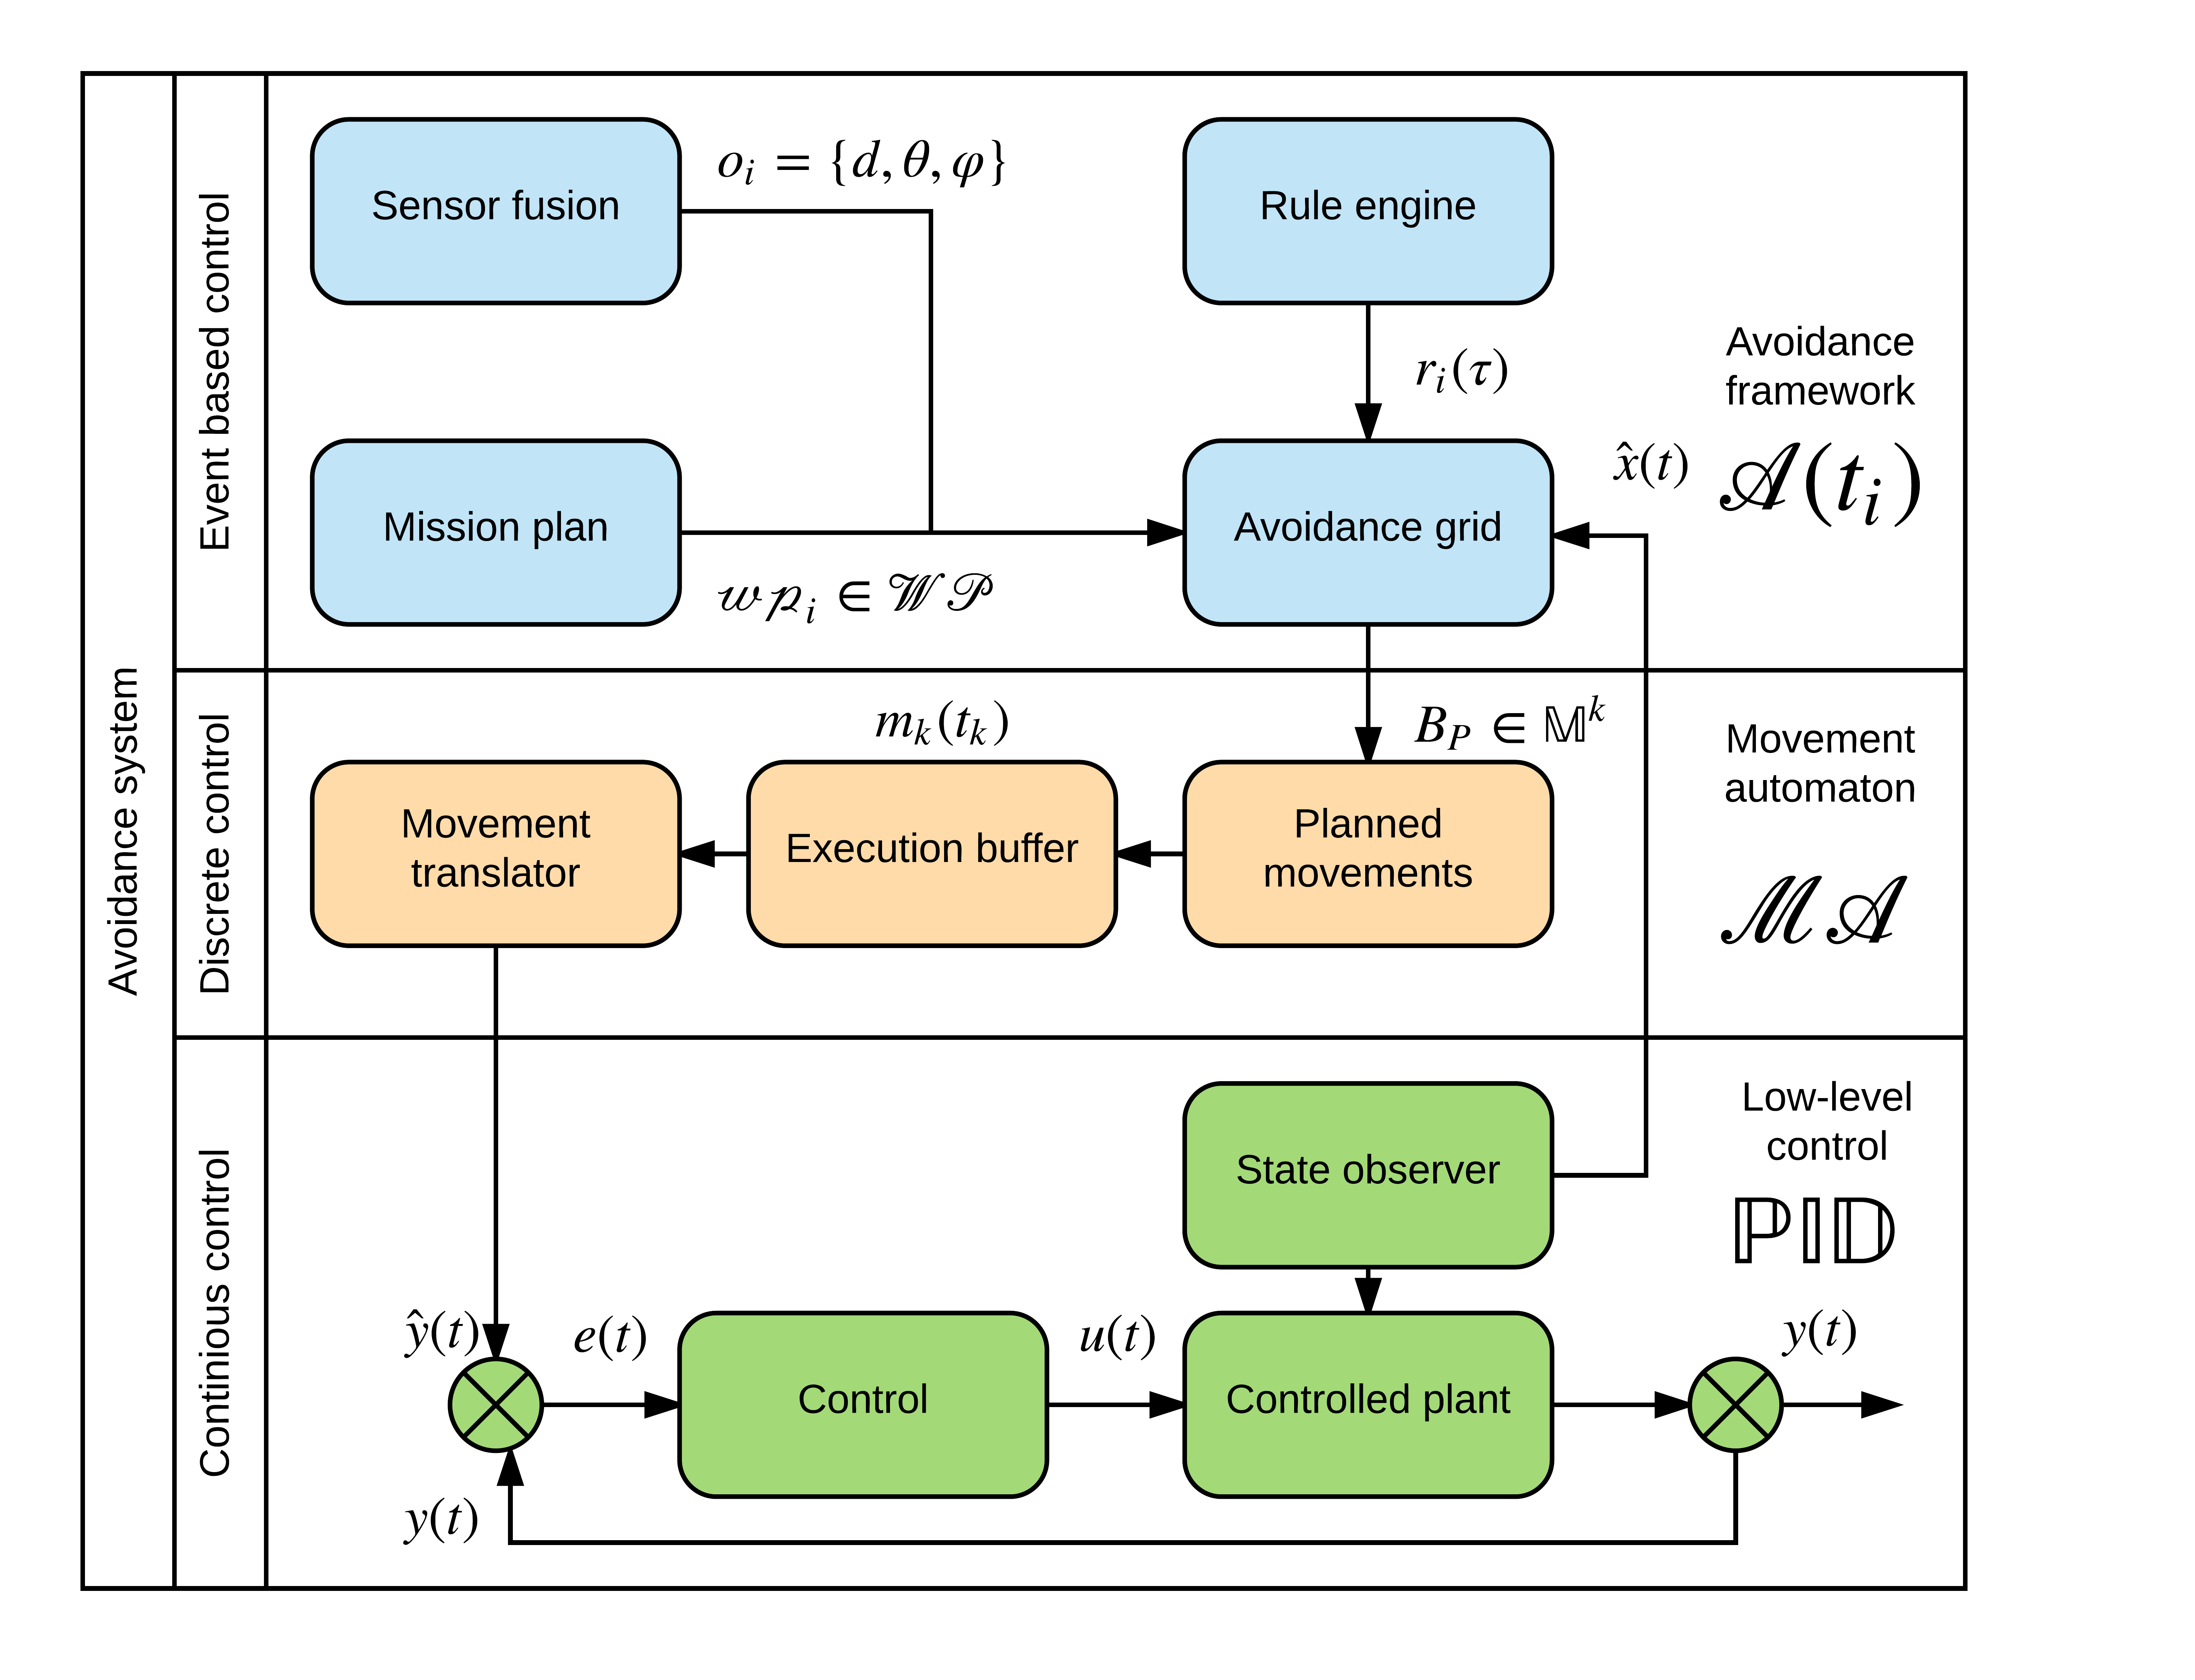
\includegraphics[width=0.8\linewidth]{\FIGDIR/TE001BlockSchemeOfControlConcept} 
    \caption{Obstacle avoidance based on Reach sets concept.}
    \label{fig:avoidanceConcept}
\end{figure}

\section{(R) Movement Automaton}\label{s:movementAutomatonTheory}

\paragraph{Idea:} The key idea is to create \emph{interface} between \emph{controlled plant} (UAV) and \emph{Avoidance Algorithm} to ensure \emph{Concept Reusability} at maximum degree.  The concept is following:

\begin{enumerate}

    \item \emph{Interface consumes} discrete command chain and guides UAS along \emph{desired trajectory}.
    
    \item \emph{Interface} can be used to \emph{predict trajectory} based on \emph{initial state} and future command chaining. 
\end{enumerate}

Frazolli provided the concept of \emph{Movement Automaton} (def. \ref{def:movementAutomaton}) a specialized type of \emph{Hybrid Automaton} (eq. \ref{eq:hybridAutomaton}), the concept is taken from his works \cite{frazzoli2001robust,frazzoli2000trajectory}. Other aspects and similarities are discussed over this chapter. 


\paragraph{Architecture:} The Movement Automaton can be seen as a consistent hierarchical abstraction of the continuous dynamics, in the sense outlined in \cite{pappas2000hierarchically}: \emph{Any sequence of movement primitives generated by the Movement Automaton results by construction in a trajectory which is executable by the full continuous system. We will give a deeper meaning to hierarchical consistency}. The implementation of our movement automaton is given in (fig.\ref{fig:avoidanceConcept}). 

\paragraph{Optimal Path Generation:} If the maneuvers are instantaneous (i.e. the UAS can transition instantaneously between two different trim trajectories), Reduction of stronger results obtained by Dubins \cite{dubins1957curves} and Reeds \cite{reeds1990optimal} concerning optimal paths for kinematic cars on the plane (see also \cite{soueres1998optimal}). 

\paragraph{Controllability:} The systems controlled by Movement Automaton (as in \cite{lavalle1998rapidly}), is controllable according to our definition, even though it is not
small-time controllable \cite{sussmann1983lie}.

\paragraph{Other Properties:} The other properties of movement automaton, like \emph{Stability, Robustness} and other important control properties are proven in \cite{frazzoli2001robust}.



\paragraph{Example:} The \emph{example} is given in (fig. \ref{fig:movementAutomatonExampleTheory}). The \emph{States} (Barrels) are connected by \emph{Transitions} (green arrows).

\emph{Hover} is neutral and \emph{initial} state, in this place the UAS stays on place and maintains altitude.

\emph{Forward flight} is when \emph{UAS} is flying in frontal direction with constant speed. The speed-up and slow-down is incorporated in \emph{Transition} between \emph{Hover} and \emph{Forward flight} states and its takes some time to execute. \emph{Transitions} between Turning states and \emph{Flight forward} state are almost instant. 

\emph{Steady turn left/right} is when \emph{UAS} is flying in frontal direction and starts steady turning left or right. 

\begin{note}
UAS in (fig. \ref{fig:movementAutomatonExampleTheory}) ignores the vertical maneuvering and it is expected to fly on horizontal plane.
\end{note}


\begin{figure}[H]
    \centering
    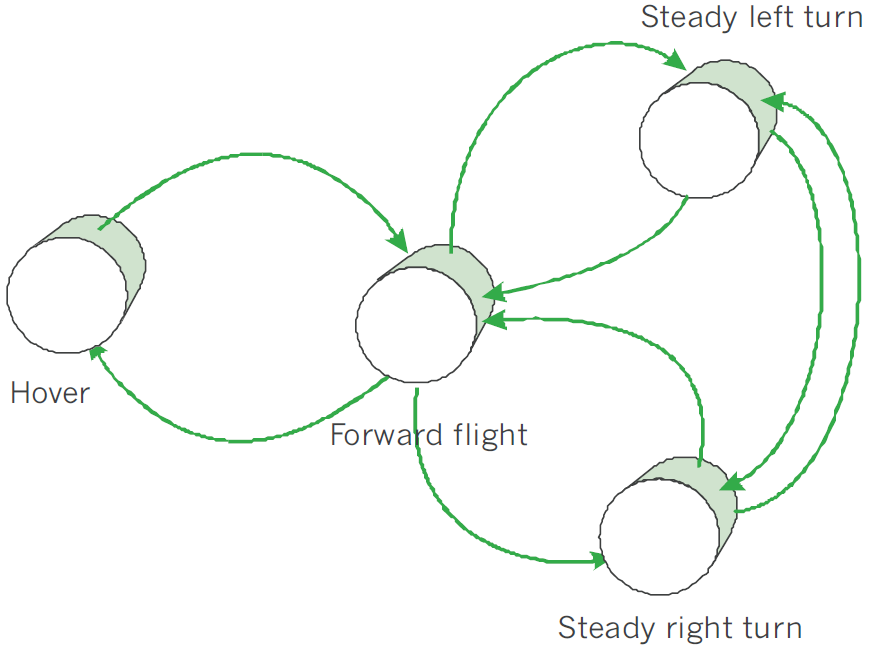
\includegraphics[width=0.55\linewidth]{\FIGDIR/TE030MovementAutomatonFrazzCite} 
    \caption{Movement Automaton for Copter UAS \cite{frazzoli2001robust}.}
    \label{fig:movementAutomatonExampleTheory}
\end{figure}

\paragraph{Used concepts:} The movement automaton is essential part of this work. Supporting the idea, that \emph{Obstacle avoidance framework} can be platform independent. 

The \emph{Movement Automaton} is used as is (sec. \ref{s:MovementAutomatonDefinitionAndProperties}). The implementation is described in (sec. \ref{s:modelMAImplementation}). The testing configuration was given in (tab. \ref{tab:testMovementOrientations}).


\section{(R) Sensor (Data) Fusion - Input Interface}\label{s:dataFusionProbabilisticModelTheory}
\paragraph{Idea:}  There is \emph{Need for abstract representation} of \emph{operational space}, which is independent of used sensors, technologies, information sources. The universal obstacle avoidance system should have \emph{portability property}. Our previous work \emph{Obstacle avoidance framework based on reach sets} \cite{gomola2017obstacle} have introduced similar concept of \emph{control interface}.

The original concept was using cell status interpretation, which was hardwired to LiDAR technology.  The new demand is to incorporate concepts of \emph{visibility}, \emph{reachibility} and \emph{obstacle probability}. The base methodst for \emph{Statistical Sensor Fusion} were outlined in \cite{gustafsson2010statistical}.

\paragraph{Key Concept:} \emph{Data fusion interface} (sec. \ref{s:dataFusionDefinition}) - interface to fuse sense data from various online, offline, cooperative, non-cooperative sources into single scalable {space and trajectory evaluation procedure}.
    
\paragraph{Related work:} \noindent UAS specific sensor fusion has been proposed by Ramsay in \cite{ramasamy2014avionics}. \emph{Next generation avoidance concept} \cite{ramasamy2014next} is introducing concept of higher level sensor fusion called \emph{data fusion}. 

The uncertainty and properties in \emph{Remotely Piloted Systems} have been discussed in \cite{chynchenko2016remotely}. The work provided concept of various performance ratings like visibility and obstacle rating, more details have been given in \cite{shmelova2016modeling}. This ratings were modeled only for operator decision making \cite{kharchenko2017modelling}, results are usable for automated decision making and space assessment. 

\emph{Probabilistic trajectory assessment} has been firstly proposed in \cite{kim2007uav} where trajectory was tracking and predicting \emph{safety properties} along. 

\emph{Game theory} viewpoint is firstly used in \cite{vidal2002probabilistic}. Probabilistic path planning using safety zones similar to cell classification of this work have been used in \cite{pfeiffer2005path}.

Probabilistic path search similar to our reach set representation using rapidly exploring path trees have been used in \cite{kothari2013probabilistically,blackmore2006probabilistic}. Relationship between classic grid search and probabilistic lattice search have been established in \cite{lavalle2004relationship}. A probabilistic approach for trajectory estimation via reduced lattice search is known from 1986 from work of Gessel \cite{gessel1986probabilistic} lattice paths were enumerated via movement sequences and similar technique is used in our reach set estimation method using movement automaton.  Pruning methods comparison and complexity can be found in \cite{esposito1997comparative}.

Overall concepts of probabilistic sets have been given by Hirota in \cite{hirota1981concepts}.  Free flight safety rating similar to our reachability concept have been presented in \cite{hoekstra2002designing}.

\paragraph{Shortcomings:} 

\begin{enumerate}
    \item \emph{Hierarchical calculation} - there is need to calculate \emph{avoidance trajectory} for incremental constraint applications. For example:
    \begin{enumerate}[a.]
        \item Calculate \emph{Minimal escape path} covering physical obstacles and intruders.
        \item Apply next level of constraints, like airspace restrictions and some virtual constraints. Then calculate path if exists, continue.
        \item Apply nice to have constraints, like non lethal weather, recalculate path.
    \end{enumerate}
    
    \item \emph{Source Reliability Evaluation} -  reliability evaluation is empirical process usually done by hand. The result aggregation is not standardized. There can be multiple sources of same rating, for example visibility, which needs to be aggregated into one.  
    
    \item \emph{Ambiguous rating definition} - There is multiple definitions especially for \emph{Reachibility rating} in works \cite{kothari2013probabilistically,blackmore2006probabilistic,gessel1986probabilistic}.
    
\end{enumerate}

\paragraph{Improvements in Our Work:}

\emph{Hierarchical calculation} is addressed in \emph{Mission Control run} (sec: \ref{s:missionControlRun}) where threats are hierarchically applied based on \emph{severity}.

\emph{Source reliability evaluation} is addressed in \emph{Static Obstacles} (sec. \ref{s:staticObstacles}) and \emph{Moving Obstacles} \ref{s:intruders}). The main rating for \emph{Detected obstacle, Map Obstacle} and \emph{Visibility} of space are established there. 

\emph{Clear rating definition} - the \emph{Reachibility} of space portion and \emph{Safety} rating for trajectory are established in \emph{Avoidance Grid Run} (sec. \ref{s:aviudabceGridRun})



\section{(R) Navigation Algorithms}\label{s:NavigationAlgorithms}
\paragraph{Idea:} The basic idea is to provide hierarchical\emph{navigation frame} with \emph{some optimal path search capabilities}. 

\paragraph{Standard Navigation:} The standard navigation is given as \emph{expected cost optimization problem} for \emph{future cost function} (eq. \ref{eq:costFunctionReachable}). The key concept of navigation algorithm was fully taken from \cite{gardi2018multi}. The decision was made based on navigation survey \cite{goerzen2010survey}. The \emph{descent} for landing is out of scope in this work, can be found in \cite{lim2018energy}. The navigation principle is roughly described in (sec. \ref{s:missionControlRun}).


\paragraph{Maze Solving Capabilities:} The \emph{maze solving capability} is usable in \emph{controlled airspace} where 2D maze solving algorithms are applicable. The notable implementation was for \emph{micro mouse robot} based on right hand rule \cite{mishra2008maze}. Flood fill algorithm is partially usable for 3D environment \cite{elshamarka2012design}. The application of \emph{maze solving} was given in case study \cite{chatelais2014maze}.

\paragraph{Hybrid Automaton Path Planning:} A hybrid automaton path planing based on $A*$ algorithm was given by Richards in \cite{richards2004hybrid}. The key idea was to use \emph{hybrid automaton} (eq. \ref{eq:hybridAutomaton}) as a reference generator. This idea was taken and formulated as \emph{Movement Automaton Predictor mode}. 

The similar idea where \emph{potential fields} were used as \emph{intruder model} and path was re-planned  based on events is given in \cite{dong2011hybrid}.

\paragraph{Mode Switch:} The \emph{Mode Switch Control} idea has been presented in \cite{ryan2005mode}. There were definition of behavioural switch between:
\begin{enumerate}
    \item \emph{Navigation Mode} - navigation control and behaviour was used.
    \item \emph{Task Specific Mode} - mode specific for tasks, authors were using modes for search and rescue. 
\end{enumerate}

This concept will be reused, the \emph{Task specific mode} will be \emph{Emergency Avoidance Mode} in Our case. The triggering events and switch conditions will be defined in (sec. \ref{s:missionControlRun}).

\paragraph{Used concepts:} The \emph{Following concepts} were used in navigation loop:
\begin{enumerate}
    \item \emph{Standard navigation} taken from \cite{gardi2018multi} minor implementation changes using offline optimization. The purpose of navigation loop is to bring us closest to the waypoint, if its reachable. Navigation example (sec. \ref{s:testRuleMixed}).
    
    \item \emph{Maze solving capabilities} partially taken as secondary functionality based on \cite{elshamarka2012design}. The purpose is the \emph{looping prevention}. The example was given in (sec. \ref{s:testMaze}) .
    
    \item \emph{Mode switch} partially taken as main feature from \cite{ryan2005mode}, the triggering events were identified and defined by author and can be found over (chapter \ref{ch:approach}).
\end{enumerate}


\section{(R) Reach Set Estimation}\label{s:ReachSetEstimationTheory}
\paragraph{Idea:} The basic idea for \emph{Discrete Reach set Estimation  method} is taken from \cite{ljungqvist2017lattice}. The focus of their work is to generate paths that are kinematically feasible. Path following controllers in order to find techniques to stabilize the system around these paths \cite{ljungqvist2016path,evestedt2016path}. 

Lattice-based planners have been deployed with great success on several robotic platforms \cite{pivtoraiko2009differentially,urmson2008william,cirillo2017videogames,tomlin2000game,chen1997game}. However, a problem with lattice-based approaches is the exponential complexity in the dimension of the state space which can limit the use for more complicated models.

The optimization problem was solved real-time by \emph{Avocado solver} \cite{houska2011acado}.

\paragraph{Example:} The \emph{example of movement lattice} is given in (fig. \ref{fig:latticeMovementPrimitivesExample}). Truck (black rectangle) is towing Trailer (red rectangle). The \emph{state} have only one \emph{reach set impacting variable} - \emph{trailer displacement}. When trailer displacement is $0^{\circ}$ (fig. \ref{fig:noDisplacementLattuce}) the lattice representation of \emph{Reach Set} is different that in case of small left/right tilt (fig. \ref{fig:displacementleftrightlattuce}).

\begin{figure}[H]
    \centering
    \begin{subfigure}{0.48\textwidth}
        \centering
        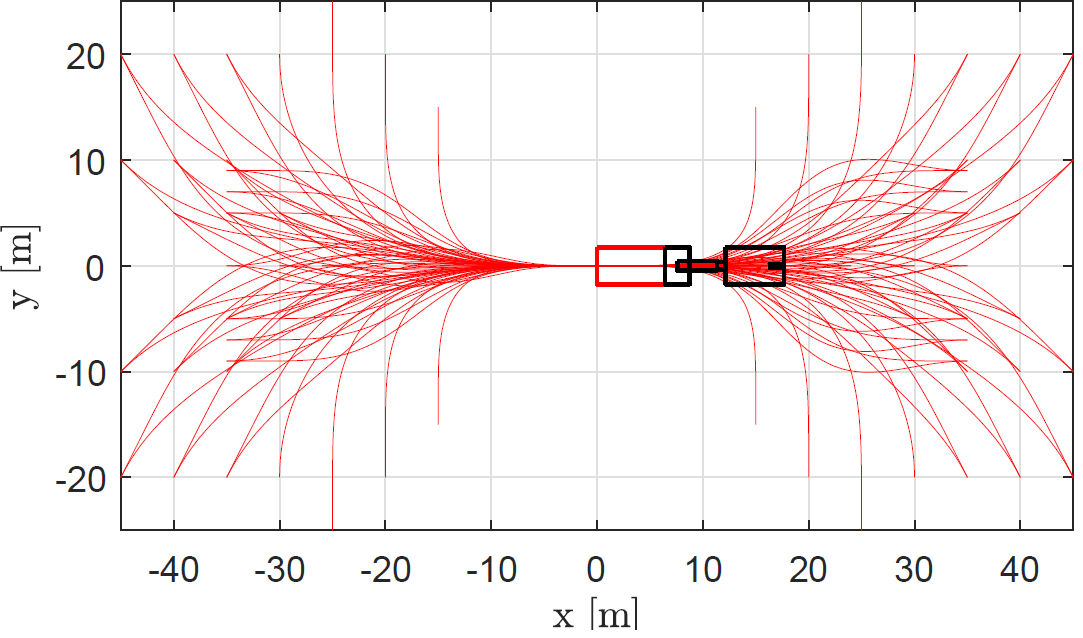
\includegraphics[width=0.9\linewidth]{\FIGDIR/TE028LattuceMovementSet01}
        \caption{Trailer displacement $0^{\circ}$.}
        \label{fig:noDisplacementLattuce}
    \end{subfigure}
    \begin{subfigure}{0.48\textwidth}
        \centering
        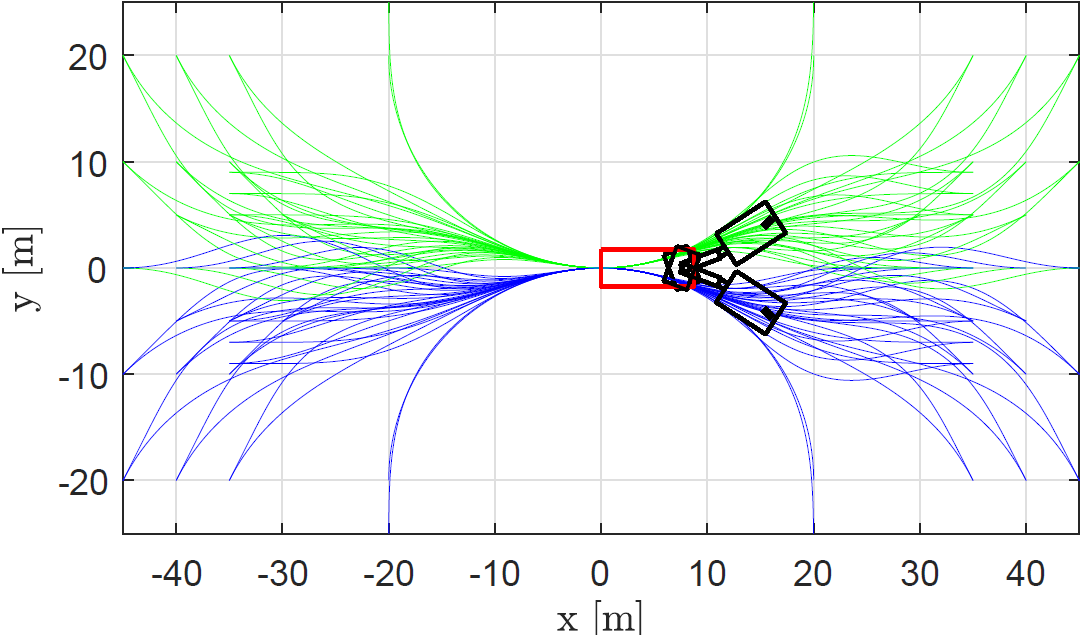
\includegraphics[width=0.9\linewidth]{\FIGDIR/TE029LattuceMovementSe02t} 
        \caption{$12^{\circ}$ (green) $-12^{\circ}$ (blue).}
        \label{fig:displacementleftrightlattuce}
    \end{subfigure}
    
    \caption{\emph{Movement set primitives} for Lattice Based Movement Planning. \cite{ljungqvist2017lattice}. }
    \label{fig:latticeMovementPrimitivesExample}
\end{figure}

\paragraph{Benefits:} Presented method of \emph{Lattice Search}  is  de-facto \emph{Reduced Reach Set Approximation} in open space for \emph{Truck-Trailer} system. 

The idea of \emph{Movement primitives} is very close to \emph{Movement Automaton} (def. \ref{def:movementAutomaton}), which can be used as \emph{control interface} effectively. 

The \emph{Constraints} of obstacle set in \emph{Known world} (sec. \ref{s:KnownWorld}) are supported to some degree.

\paragraph{Shortcomings:} There are following shortcomings which were identified in this approach:
\begin{enumerate}
    \item \emph{Limited system dimension} - given method works in \emph{real time} only if dimension of \emph{system state space} does not exceed $4^{th}$  rank.
    
    \item \emph{Real time optimization} - real time optimization is main cause of \emph{limited system dimension}. If the decision time can be discrete (which movement automaton enforces) then offline optimization  can be used. 
    
    \item \emph{Continuous space disparity} - the example (fig. \ref{fig:latticeMovementPrimitivesExample}) shows there are member variables of \emph{State Space} which significantly impacts the shape of lattice (reach set estimation). This is not a problem in real-time environment. The discretization of \emph{Time domain} raises this as a shortcoming.
    
    \item \emph{Trajectory Tracking} - approach generates \emph{Continuous Domain} reference signal. For \emph{Discrete Domain} it is necessary to address this issue.
\end{enumerate}

\paragraph{Improvements in Our Work:}

\emph{Limited system dimension} - the discretization due the higher system dimension and  increased maneuver complexity goes hand-in-hand with \emph{pre-calculation} of the \emph{Reach Set}. This shortcoming is addressed in (sec. \ref{s:constrainedTrajectoryExpansion}).

\emph{Real time optimization} -  replaced by \emph{Discrete offline optimization problem}. The \emph{general cost function} is given in (eq. \ref{eq:costFunctionReachable}). The optimization problem solved in this work is defined in (eq. \ref{eq:trajectoryTrackingOptimalizaitonProblem}).

\emph{Continuous space disparity} - The \emph{pre-calculated reach set estimation} can be valid with small \emph{marginal error} for some region in \emph{system state space}. The dynamic method for state space segmentation can be used \cite{takahashi1996reasonable}. This aspect is not addressed in this work, because it is strongly depending on the system behind movement automaton. 

\emph{Trajectory Tracking} - The \emph{movement automaton} (def. \ref{def:movementAutomaton}) in Control Mode can be used to track reference trajectory in form of \emph{Movement Buffer}(def. \ref{def:MovementBuffer}). Other option is to use \emph{thick waypoint trajectory tracking for UAV} like in \cite{kaminer1998trajectory} or \cite{murillo2015generalized}. The work will use only \emph{Movement Automaton} as controller/predictor. 




\section{(R) Testing Framework}\label{s:TestingFrameworkTheory}

\paragraph{Idea:} \emph{Reuse LSTS toolchain architecture} for DAA testing framework.

\paragraph{LSTS Toolchain:} Software architecture used in modern unmanned aerial vehicles must be system independent and scalable. Writing own control software for unmanned aerial vehicle and ground station is unthinkable in current state of art.  Most notable framework for unmanned aerial vehicle development is LSTS tool chain from University of Porto \cite{merani2011underwater}. This tool chain is widespread in other universities and multiple independent applications are based on it \cite{rajan2013towards}.

\begin{figure}[H]
    \centering
    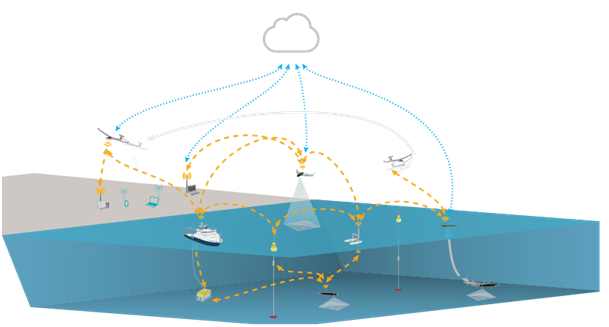
\includegraphics[width=0.9\linewidth]{\FIGDIR/TE036LSTSDeployment}
    \caption{Example of LSTS toolchain deployment in real environment \cite{pinto2006neptus}}
    \label{fig:lstsdeployment}
\end{figure}

Example of software architecture implementation is shown in figure \ref{fig:lstsdeployment} LSTS HUB (cloud iconography) is collecting all important data from currently executing missions. Data are transferred via REST API (dotted blue lines) to HUB.  Commanded vehicles can be unmanned copters, planes, ships, submarines or floating sensors compounds. Each vehicle has installed DUNE which is responsible for vehicle command and ground control station communication. Deployment, range of command and status messages can vary. Ground station can be implemented on personal computer (any platform) in NEPTUS environment or mobile platform (Android OS) in ACCU environment. Ground station environments are customizable and open source. Layout of ground station can be customized to need of current mission via plugins or console configuration. Vehicles and ground stations are communicating via IMC protocol (orange dashed lines). Communication channel is platform independent.


\textit{Glued} is a Debian-based open source operating system which was initially released in 2010.  Over the years it has become fairly widespread and been provided continuous updates.  Meanwhile, a notable development community has emerged, where advice and support can be received as more applications are investigated. Some of the merits of the operating system are its reliability and customizability. Operation system is developed for unmanned autonomous vehicles. It is widely used in air, sea and land vehicles. Customization allows the operating system to be tailored to the specific usage. For this purpose, this includes stripping off functionality which is not required, thus releasing resources to be focused on the essential tasks. Glued is the operating system favored by the Beaglebone development community, and thus there exist considerable amounts of helpful documentation for this set-up.

\textit{DUNE: Unified Navigational Environment} is an on-board software solution for unmanned vehicles. Multiple applications already run on this software. Almost any extension can be added to this to this environment. The software solution provides means for interacting with the connected components as well as control, navigation, supervision and plan execution.  It is both CPU architecture independent and OS independent.  It is written in C++ and developed by LSTS: Underwater Systems and Technology Laboratory.

\textit{Neptus} \cite{pinto2006neptus,dias2006mission,dias2005neptus} is a command and control software operated from a ground station. It is designed to operate well together with Dune and was also developed by LSTS. Neptus provides tools for remotely monitoring UAVs and assigning plans and commands in real-time missions, supporting multiple connections dynamically. Furthermore, it provides possibilities for both simulating missions and reviewing previously performed operations. This is presented in a customizable interface equipped with map layers and control panels. It is written in Java and available for both Windows and Linux systems.

The \textit{Inter-Module Communication} \cite{martins2009imc} (IMC) protocol was developed by LSTS to provide reliable communication between the systems.  The protocol is message-oriented, such that messages can be sent and received from a bus which connects independently run threads or systems.  Thus it functions as a method of communication between tasks internally in Dune, and can also be passed to and from other vehicles or computers running Dune or Neptus.  IMC is platform independent at multiple messages have been already developed and supported by both DUNE and Neptus (around 400 status/command messages).

\textit{HUB} is communication hub for data dissemination and situation awareness. This module is responsible for complex mission execution, when cooperation of multiple pilots/vehicles is required. This module can be imagined as airport tower center, which is monitoring all flights in airport (operation site) area. This tool implements REST API for communication between various ground stations and operating vehicles.

\paragraph{Movement Automaton Control} Marconi used \emph{hybrid automaton} with forced \emph{State Switch} via buffer \cite{marconi2009control}. The key concept is that \emph{Automata} state switch is forced as \emph{external source command}. Our \emph{Movement Automaton} implementation know only \emph{forced state switch} like in \cite{frazzoli2000trajectory}. 

\paragraph{Used concepts:} Most of the architecture was re-used in our approach, the concept of \emph{Rule engine} (sec. \ref{sec:ruleEngine}) was introduced to cover missing \emph{UTM} related functionality. The implementation in Matlab was influenced by Alessandeti works \cite{allesandeti2016virtualArena,alessandrettinotes}. The other aircraft dynamic and control related concepts were taken from  \cite{stevens2015aircraft}.

\section{(R) UTM Services}\label{s:utmServicesTheory}
\paragraph{Idea:} Take the Airbus UTM concept \cite{airbusUTM2018blueprint} combine it with \emph{EUROCONTROL} concept \cite{andrewhately2018} to obtain legal framework. \emph{Provide conflict resolution functionality} for \emph{Controlled Airspace}:
\begin{enumerate}
    \item \emph{Collision Detection} - define minimal required functionality for collision detection.
    \item \emph{Collision Resolution} - implement \emph{Rules of the Air} \cite{standard1986recommended}.
\end{enumerate}

The \emph{implementation} of \emph{UTM services} described in (sec. \ref{sec:UTM}) is given in (sec. \ref{sec:UASTrafficManagement}).

\paragraph{UTM Operation Modes:} \emph{defined in } \cite{airbusUTM2018blueprint} are following:
\begin{enumerate}
    \item \emph{Free route} (fig. \ref{fig:UTMFreeRouteMode}) is when aircraft can fly any path, so long as their planned path is coordinated with and de-conflicted from the paths of other aircraft by a traffic manager and approved based on calculated risk. Free routing is being introduced worldwide, such as free route airspace. This allows commercial flights to freely plan their route through participating sectors during cruise. There is less freedom for an aircraft in this situation than in basic flight, since its request may be rejected.
    
    \item\emph{Corridors} (fig. \ref{fig:CorridorMode})  are defined volumes in space, useful for managing airspace in high demand or to manage traffic flow and separation. Coordination is necessary to ensure safety in this airspace. A corridor may take on many different shapes. Aircraft are often guided inside corridors using predetermined routes analogous to approach procedures used worldwide today.
    
    \item\emph{Fixed route} (fig. \ref{fig:fixedRoute}) are used to ensure safety when there is high traffic density or in any location where structure is required to ensure safe operations. This could include locations such as airports or warehouses. These routes could be constructed or modified dynamically based on calculated risk. The most restrictive version is a predetermined path, where the only variable is when an aircraft is at a specific point in the path.
\end{enumerate}

\begin{figure}[H]
    \centering
    \begin{subfigure}{0.32\textwidth}
        \centering
        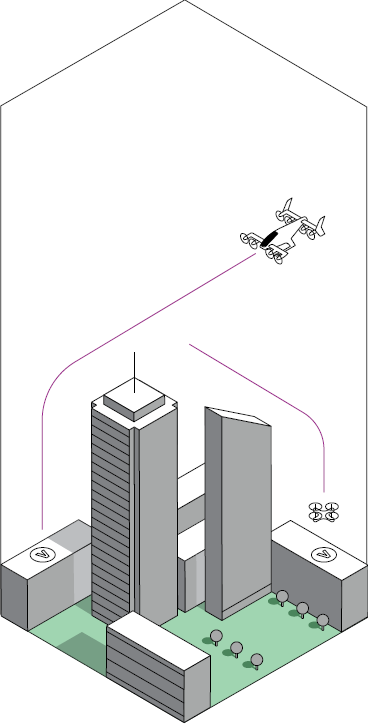
\includegraphics[width=0.9\linewidth]{\FIGDIR/TE032FreeRoute}
        \caption{Free route.}
        \label{fig:UTMFreeRouteMode}
    \end{subfigure}
    \begin{subfigure}{0.32\textwidth}
        \centering
        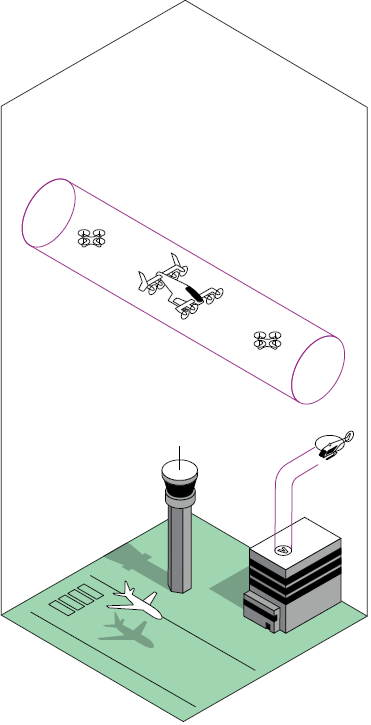
\includegraphics[width=0.9\linewidth]{\FIGDIR/TE034Corridors} 
        \caption{Corridors.}
        \label{fig:CorridorMode}
    \end{subfigure}
    \begin{subfigure}{0.32\textwidth}
        \centering
        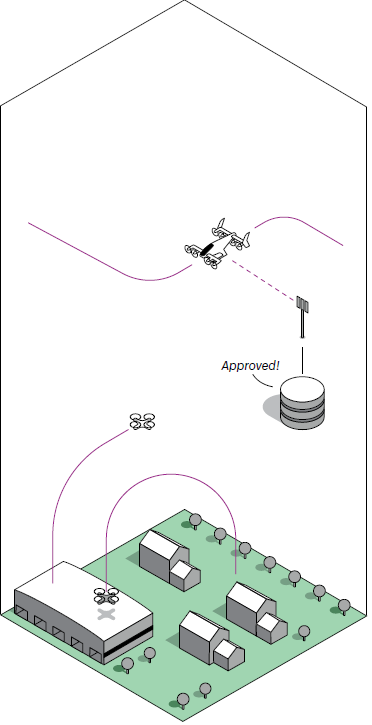
\includegraphics[width=0.9\linewidth]{\FIGDIR/TE035FixedRoute} 
        \caption{Fixed route.}
        \label{fig:fixedRoute}
    \end{subfigure}
    
    \caption{UTM Operation Modes.}
    \label{fig:utmOperationModes}
\end{figure}

\paragraph{Used Concepts:} The implementation of our UTM services  is focused on \emph{Free route mode} (fig. \ref{fig:UTMFreeRouteMode}). The \emph{Corridors} and \emph{Fixed routes} are just additional \emph{space/time constraints}.
    	\section{\secState{R}Movement Control}\label{s:movementAutomatonTheory}

\paragraph{Idea:} The key idea is to create \emph{interface} between \emph{controlled plant} (UAS) and \emph{Avoidance Algorithm} to ensure \emph{Concept Reusability} at maximum degree.  The concept is the following:

\begin{enumerate}

    \item \emph{Interface consumes} discrete command chain and guides UAS along the \emph{desired trajectory}.
    
    \item \emph{An interface} can be used to \emph{predict trajectory} based on \emph{initial state} and future command chaining. 
\end{enumerate}


\paragraph{Frazzoli Movement Automaton:} The following paragraph strongly follows Frazzoli work \cite{frazzoli2001robust} (sec 3.1-3.5). Frazolli provided the concept of \emph{Movement Automaton} (def. \ref{def:movementAutomaton}) a specialized type of \emph{Hybrid Automaton} (eq. \ref{eq:hybridAutomaton}), the concept is taken from his works \cite{frazzoli2001robust,frazzoli2000trajectory}. Other aspects and similarities are discussed in this chapter. 


The approach was proposed to reduce the \emph{computational complexity problem} of \emph{motion planning}. The quantization of the system dynamics is done through restriction of feasible nominal system trajectories to the \emph{family of time parametrized curves}. These can be obtained by the interconnection of trajectory primitives.

\emph{Trajectory primitives} are repeatable portions of trajectory (def. \cite{frazzoli2001robust}.3.1). The trajectory primitives are interconnected by \emph{transitions} to create maneuvers (movements) (def. \cite{frazzoli2001robust}.3.3). 

By combining movements as a set of trim trajectories the trajectory can be represented as a set of discrete time bounded commands. This is summarized in the definition (def. \cite{frazzoli2001robust}.3.4) based on \emph{hybrid automaton definition} (sec. \ref{s:HybridAutomaton}).
\begin{definition}[Maneuver Automaton] A maneuver automaton over a mechanical control system $S$, with symmetry group $H$ is described by the following objects:

\begin{enumerate}
    \item A finite set of indices $Q = Q_T \cup Q_M \in \N$, where the subscript T relates to trim trajectories, and the subscript M relates to maneuvers;
    
    \item A finite set of trim trajectory parameters $\left(\bar{g},\bar{\xi},\bar{u}\right)_q$; with $q\in Q_T$.
    
    \item A finite set of maneuver parameters, and state and control trajectories $\left(T,u,\phi\right)_q$, with $q\in Q_M$.
    
    \item The maps $Previous: Q_M\to Q_T $, and, $Next: Q_M \to Q_T$ such that $Previous(q)$ and $Next(q)$ give, respectively, the index of the trim trajectories from which the maneuver $q$ starts and ends.
    
    \item A discrete state $q \in Q$.
    
    \item A continuous state, denoting the position on the symmetry group, $h \in H$.
    
    \item A clock state $\theta \in \R$, which evolves according to $\dot{\theta}=1$, and which is reset after each switch on $q$.
\end{enumerate}
\begin{note}
    It is apparent that decisions can be made about the future evolution of the system only when the system is executing a trim trajectory (that is, the discrete state is in one of the nodes in the graph). While executing a maneuver the system is committed to it and must keep executing the maneuver until its completion. As a consequence, for motion planning and control design purposes, one can concentrate the study of the evolution of the system on and between nodes.
\end{note}
\end{definition}


\paragraph{Architecture:} The Movement Automaton can be seen as a consistent hierarchical abstraction of the continuous dynamics, in sense outlined in \cite{pappas2000hierarchically}: \emph{Any sequence of movement primitives generated by the Movement Automaton results by construction in a trajectory which is executable by the full continuous system. We will give a deeper meaning to hierarchical consistency}. 

\paragraph{Optimal Path Generation:} If the maneuvers are instantaneous (i.e., the UAS can transition instantaneously between two different trim trajectories), Reduction of stronger results obtained by Dubins \cite{dubins1957curves} and Reeds \cite{reeds1990optimal} concerning optimal paths for kinematic cars on the plane (see also \cite{soueres1998optimal}). 

\paragraph{Controllability:} The systems controlled by Movement Automaton (as in \cite{lavalle1998rapidly}), is controllable according to our definition, even though it is not
small-time controllable \cite{sussmann1983lie}.

\paragraph{Other Properties:} The other properties of movement automaton, like \emph{Stability, Robustness} and other important control properties are proven in \cite{frazzoli2001robust}.


\paragraph{Example:} The \emph{example} is given in (fig. \ref{fig:movementAutomatonExampleTheory}). The \emph{States} (Barrels) are connected by \emph{Transitions} (green arrows).

\emph{Hover} is the neutral and \emph{initial} state, in this place the UAS stays on place and maintains altitude.

\emph{Forward flight} is when \emph{UAS} is flying in frontal direction with constant speed. The speed-up and slow-down are incorporated in \emph{Transition} between \emph{Hover} and \emph{Forward flight} states, and it takes some time to execute. \emph{Transitions} between Turning states and \emph{Flight forward} state are almost instant. 

\emph{Steady turn left/right} is when \emph{UAS} is flying in the frontal direction and starts steady turning left or right. 

\begin{note}
UAS in (fig. \ref{fig:movementAutomatonExampleTheory}) ignores the vertical maneuvering, and it is expected to fly on horizontal plane.
\end{note}


\begin{figure}[H]
    \centering
    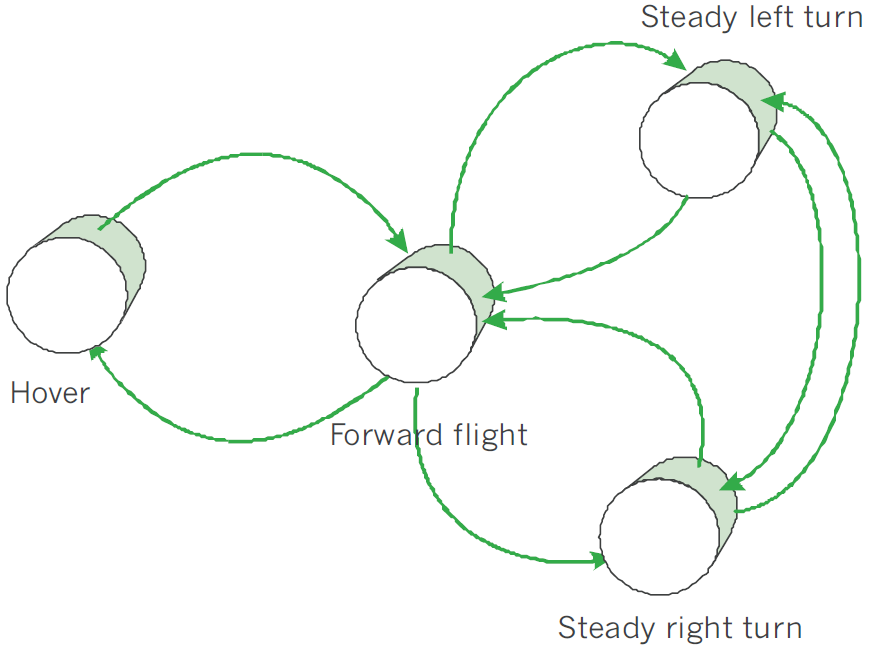
\includegraphics[width=0.55\linewidth]{\FIGDIR/TE030MovementAutomatonFrazzCite} 
    \caption{Movement Automaton for Copter UAS \cite{frazzoli2001robust}.}
    \label{fig:movementAutomatonExampleTheory}
\end{figure}

\begin{note}
The \emph{Movement Automaton} is used as with modification (sec. \ref{s:MovementAutomatonDefinitionAndProperties}). The implementation is described in (sec. \ref{s:modelMAImplementation}). The testing configuration was given in (tab. \ref{tab:testMovementOrientations}).
\end{note}


    	\section{\secState{R}Surveillance}\label{s:dataFusionProbabilisticModelTheory}
\paragraph{Idea:}  There is a \emph{need for the abstract representation} of \emph{operational space}, which is independent of used sensors, technologies, information sources. The universal obstacle avoidance system should be \emph{portable} between various platforms. Our previous work \emph{Obstacle avoidance framework based on reach sets} \cite{gomola2017obstacle} has introduced a concept of the \emph{control interface}. The concept of \emph{control interface} increases portability of the solution.

The original concept used cell status interpretation (boolean values), which is hardwired to LiDAR technology. The basic methods for \emph{Statistical Sensor Fusion} were outlined in \cite{gustafsson2010statistical}. The result of the application of the method is \emph{data fusion interface} (sec. \ref{s:dataFusionDefinition}) - interface to fuse sense data from various online, offline, cooperative, non-cooperative sources into single scalable {space and trajectory evaluation procedure}.
    
\paragraph{Related work:} \noindent UAS specific sensor fusion has been proposed by Ramsay in \cite{ramasamy2014avionics}. \emph{Next generation avoidance concept} \cite{ramasamy2014next} is introducing concept of higher-level sensor fusion called \emph{data fusion}. 

The uncertainty and properties in \emph{Remotely Piloted Systems} have been discussed in \cite{chynchenko2016remotely}. The work provided the concept of various performance ratings like visibility and obstacle rating; more details have been given in \cite{shmelova2016modeling}. These ratings were modeled only for operator decision making \cite{kharchenko2017modelling}, results are usable for automated decision making and space assessment. 





    	\section{\secState{R}Navigation Algorithms}\label{s:NavigationAlgorithms}
\paragraph{Idea:} The basic idea is to provide hierarchical\emph{navigation frame} with \emph{some optimal path search capabilities}. 

\paragraph{Standard Navigation:} The standard navigation is given as \emph{expected cost optimization problem} for \emph{future cost function} (eq. \ref{eq:costFunctionReachable}). The key concept of navigation algorithm was fully taken from \cite{gardi2018multi}. The decision was made based on navigation survey \cite{goerzen2010survey}. The \emph{descent} for landing is out of scope in this work, can be found in \cite{lim2018energy}. The navigation principle is roughly described in (sec. \ref{s:missionControlRun}).


\paragraph{Maze Solving Capabilities:} The \emph{maze solving capability} is usable in \emph{controlled airspace} where 2D maze solving algorithms are applicable. The notable implementation was for \emph{micro mouse robot} based on right hand rule \cite{mishra2008maze}. Flood fill algorithm is partially usable for 3D environment \cite{elshamarka2012design}. The application of \emph{maze solving} was given in case study \cite{chatelais2014maze}.

\paragraph{Hybrid Automaton Path Planning:} A hybrid automaton path planing based on $A*$ algorithm was given by Richards in \cite{richards2004hybrid}. The key idea was to use \emph{hybrid automaton} (eq. \ref{eq:hybridAutomaton}) as a reference generator. This idea was taken and formulated as \emph{Movement Automaton Predictor mode}. 

The similar idea where \emph{potential fields} were used as \emph{intruder model} and path was re-planned  based on events is given in \cite{dong2011hybrid}.

\paragraph{Mode Switch:} The \emph{Mode Switch Control} idea has been presented in \cite{ryan2005mode}. There were definition of behavioural switch between:
\begin{enumerate}
    \item \emph{Navigation Mode} - navigation control and behaviour was used.
    \item \emph{Task Specific Mode} - mode specific for tasks, authors were using modes for search and rescue. 
\end{enumerate}

This concept will be reused, the \emph{Task specific mode} will be \emph{Emergency Avoidance Mode} in Our case. The triggering events and switch conditions will be defined in (sec. \ref{s:missionControlRun}).

\paragraph{Used concepts:} The \emph{Following concepts} were used in navigation loop:
\begin{enumerate}
    \item \emph{Standard navigation} taken from \cite{gardi2018multi} minor implementation changes using offline optimization. The purpose of navigation loop is to bring us closest to the waypoint, if its reachable. Navigation example (sec. \ref{s:testRuleMixed}).
    
    \item \emph{Maze solving capabilities} partially taken as secondary functionality based on \cite{elshamarka2012design}. The purpose is the \emph{looping prevention}. The example was given in (sec. \ref{s:testMaze}) .
    
    \item \emph{Mode switch} partially taken as main feature from \cite{ryan2005mode}, the triggering events were identified and defined by author and can be found over (chapter \ref{ch:approach}).
\end{enumerate}



    	\section{\secState{R}Reach Set Estimation}\label{s:ReachSetEstimationTheory}
\paragraph{Idea:} The basic idea for \emph{Discrete Reach set Estimation  method} is taken from \cite{ljungqvist2017lattice}. The focus of their work is to generate paths that are kinematically feasible. Path following controllers in order to find techniques to stabilize the system around these paths \cite{ljungqvist2016path,evestedt2016path}. 

Lattice-based planners have been deployed with great success on several robotic platforms \cite{pivtoraiko2009differentially,urmson2008william,cirillo2017videogames,tomlin2000game,chen1997game}. However, a problem with lattice-based approaches is the exponential complexity in the dimension of the state space which can limit the use for more complicated models.

The optimization problem was solved real-time by \emph{Avocado solver} \cite{houska2011acado}.

\paragraph{Example:} The \emph{example of movement lattice} is given in (fig. \ref{fig:latticeMovementPrimitivesExample}). Truck (black rectangle) is towing Trailer (red rectangle). The \emph{state} have only one \emph{reach set impacting variable} - \emph{trailer displacement}. When trailer displacement is $0^{\circ}$ (fig. \ref{fig:noDisplacementLattuce}) the lattice representation of \emph{Reach Set} is different that in case of small left/right tilt (fig. \ref{fig:displacementleftrightlattuce}).

\begin{figure}[H]
    \centering
    \begin{subfigure}{0.48\textwidth}
        \centering
        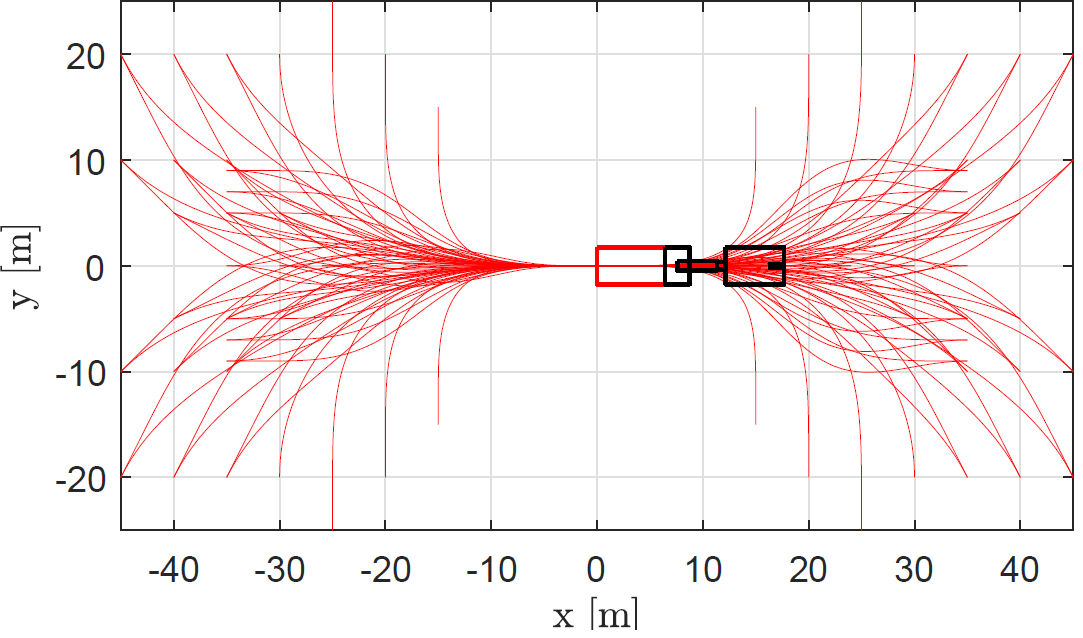
\includegraphics[width=0.9\linewidth]{\FIGDIR/TE028LattuceMovementSet01}
        \caption{Trailer displacement $0^{\circ}$.}
        \label{fig:noDisplacementLattuce}
    \end{subfigure}
    \begin{subfigure}{0.48\textwidth}
        \centering
        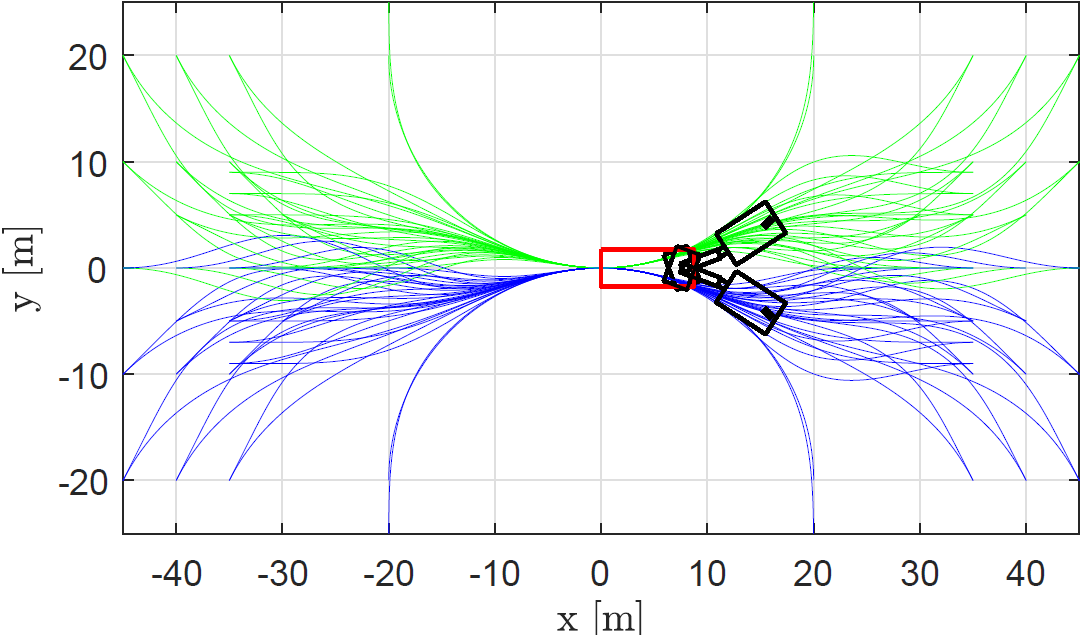
\includegraphics[width=0.9\linewidth]{\FIGDIR/TE029LattuceMovementSe02t} 
        \caption{$12^{\circ}$ (green) $-12^{\circ}$ (blue).}
        \label{fig:displacementleftrightlattuce}
    \end{subfigure}
    
    \caption{\emph{Movement set primitives} for Lattice Based Movement Planning. \cite{ljungqvist2017lattice}. }
    \label{fig:latticeMovementPrimitivesExample}
\end{figure}

\paragraph{Benefits:} Presented method of \emph{Lattice Search}  is  de-facto \emph{Reduced Reach Set Approximation} in open space for \emph{Truck-Trailer} system. 

The idea of \emph{Movement primitives} is very close to \emph{Movement Automaton} (def. \ref{def:movementAutomaton}), which can be used as \emph{control interface} effectively. 

The \emph{Constraints} of obstacle set in \emph{Known world} (sec. \ref{s:KnownWorld}) are supported to some degree.

\paragraph{Shortcomings:} The lattice search approach has following shortcoming:
\begin{enumerate}
    \item \emph{Limited system dimension} - given method works in \emph{real time} only if dimension of \emph{system state space} does not exceed $4^{th}$  rank.
    
    \item \emph{Real time optimization} - real time optimization is main cause of \emph{limited system dimension}. If the decision time can be discrete (which movement automaton enforces) then offline optimization  can be used. 
    
    \item \emph{Continuous space disparity} - the example (fig. \ref{fig:latticeMovementPrimitivesExample}) shows there are member variables of \emph{State Space} which significantly impacts the shape of lattice (reach set estimation). This is not a problem in real-time environment. The discretization of \emph{Time domain} raises this as a shortcoming.
    
    \item \emph{Trajectory Tracking} - approach generates \emph{Continuous Domain} reference signal. For \emph{Discrete Domain} it is necessary to address this issue.
\end{enumerate}

 





    	\section{Software Testing}\label{s:TestingFrameworkTheory}

\paragraph{Idea:} \emph{Reuse LSTS toolchain architecture} for DAA testing framework.

\paragraph{LSTS Toolchain:} Software architecture used in modern unmanned aerial vehicles must be system independent and scalable. Writing own control software for unmanned aerial vehicle and ground station is unthinkable in the current state of the art.  Most notable framework for unmanned aerial vehicle development is the LSTS toolchain from University of Porto \cite{merani2011underwater}. This toolchain is widespread in other universities, and multiple independent applications are based on it \cite{rajan2013towards}.

\begin{figure}[H]
    \centering
    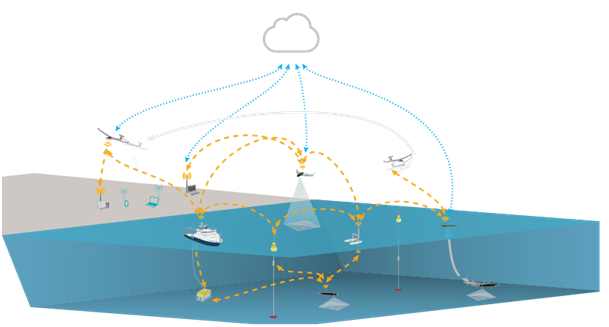
\includegraphics[width=0.9\linewidth]{\FIGDIR/TE036LSTSDeployment}
    \caption{Example of LSTS toolchain deployment in a real environment \cite{pinto2006neptus}}
    \label{fig:lstsdeployment}
\end{figure}

Example of software architecture implementation is shown in figure \ref{fig:lstsdeployment} LSTS HUB (cloud iconography) is collecting all important data from currently executing missions. Data are transferred via REST API (dotted blue lines) to HUB.  Commanded vehicles can be unmanned copters, planes, ships, submarines or floating sensors compounds. Each vehicle has installed DUNE which is responsible for vehicle command and ground control station communication. Deployment, a range of command and status messages can vary. The ground station can be implemented on a personal computer (any platform) in NEPTUS environment or mobile platform (Android OS) in ACCU environment. Ground station environments are customizable and open source. The layout of the ground station can be customized to need of current mission via plugins or console configuration. Vehicles and ground stations are communicating via IMC protocol (orange dashed lines). The communication channel is platform independent.


\textit{Glued} is a Debian-based open source operating system which was initially released in 2010.  Over the years it has become fairly widespread and been provided continuous updates.  Meanwhile, a notable development community has emerged, where advice and support can be received as more applications are investigated. Some of the merits of the operating system are its reliability and customizability. Operation system is developed for unmanned autonomous vehicles. It is widely used in air, sea and land vehicles. Customization allows the operating system to be tailored to the specific usage. For this purpose, this includes stripping off functionality which is not required, thus releasing resources to be focused on the essential tasks. Glued is the operating system favored by the Beaglebone development community, and thus there exist considerable amounts of helpful documentation for this set-up.

\textit{DUNE: Unified Navigational Environment} is an onboard software solution for unmanned vehicles. Multiple applications already run on this software. Almost any extension can be added to this to this environment. The software solution provides a means for interacting with the connected components as well as control, navigation, supervision and plan execution.  It is both CPU architecture independent and OS independent.  It is written in C++ and developed by LSTS: Underwater Systems and Technology Laboratory.

\textit{Neptus} \cite{pinto2006neptus,dias2006mission,dias2005neptus} is a command and control software operated from a ground station. It is designed to operate well together with Dune and was also developed by LSTS. Neptus provides tools for remotely monitoring UAVs and assigning plans and commands in real-time missions, supporting multiple connections dynamically. Furthermore, it provides possibilities for both simulating missions and reviewing previously performed operations. This is presented in a customizable interface equipped with map layers and control panels. It is written in Java and available for both Windows and Linux systems.

The \textit{Inter-Module Communication} \cite{martins2009imc} (IMC) protocol was developed by LSTS to provide reliable communication between the systems.  The protocol is message-oriented, such that messages can be sent and received from a bus which connects independently run threads or systems.  Thus it functions as a method of communication between tasks internally in Dune, and can also be passed to and from other vehicles or computers running Dune or Neptus.  IMC is platform independent at multiple messages have been already developed and supported by both DUNE and Neptus (around 400 status/command messages).

\textit{HUB} is communication hub for data dissemination and situation awareness. This module is responsible for complex mission execution when cooperation of multiple pilots/vehicles is required. This module can be imagined as an airport tower (traffic control) center, which is monitoring all flights in the airport (operation site) area.

\paragraph{Movement Automaton Control} Marconi used \emph{hybrid automaton} with forced \emph{State Switch} via buffer \cite{marconi2009control}. The key concept is that \emph{Automata} state switch is forced as \emph{external source command}. Our \emph{Movement Automaton} implementation knows only \emph{forced state switch} like in \cite{frazzoli2000trajectory}. 

\paragraph{Used concepts:} Most of the architecture was re-used in our approach, the concept of \emph{Rule engine} (sec. \ref{sec:ruleEngine}) was introduced to cover missing \emph{UTM} related functionality. The implementation in Matlab was influenced by Alessandeti works \cite{allesandeti2016virtualArena,alessandrettinotes}. The other aircraft dynamic and control related concepts were taken from  \cite{stevens2015aircraft}.


    	\section{\secState{R}UTM Services}\label{s:utmServicesTheory}
\paragraph{Idea:} Take the Airbus UTM concept \cite{airbusUTM2018blueprint} combine it with \emph{EUROCONTROL} concept \cite{andrewhately2018} to obtain a legal framework. \emph{Provide conflict resolution functionality} for \emph{Controlled Airspace}:
\begin{enumerate}
    \item \emph{Collision Detection} - define minimal required functionality for collision detection.
    \item \emph{Collision Resolution} - implement \emph{Rules of the Air} \cite{standard1986recommended}.
\end{enumerate}

\begin{figure}[H]
    \centering
    \begin{subfigure}{0.32\textwidth}
        \centering
        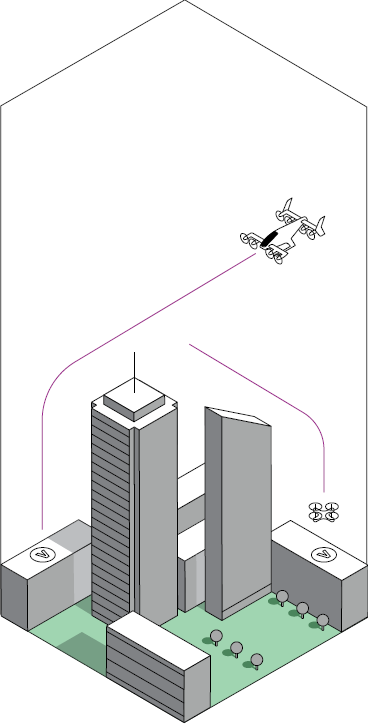
\includegraphics[width=0.9\linewidth]{\FIGDIR/TE032FreeRoute}
        \caption{Free route.}
        \label{fig:UTMFreeRouteMode}
    \end{subfigure}
    \begin{subfigure}{0.32\textwidth}
        \centering
        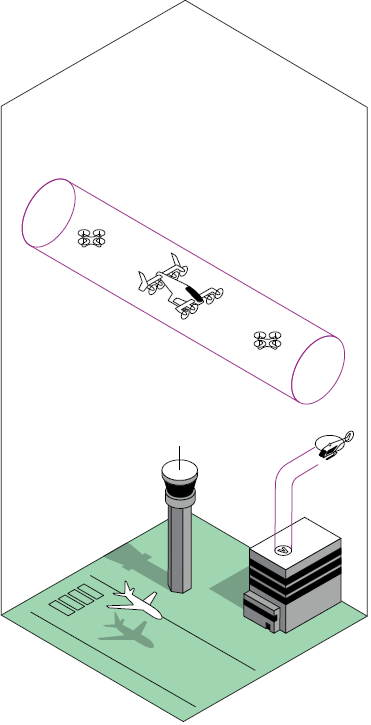
\includegraphics[width=0.9\linewidth]{\FIGDIR/TE034Corridors} 
        \caption{Corridors.}
        \label{fig:CorridorMode}
    \end{subfigure}
    \begin{subfigure}{0.32\textwidth}
        \centering
        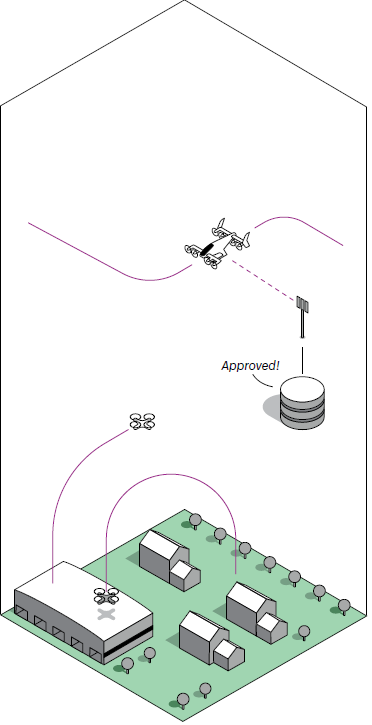
\includegraphics[width=0.9\linewidth]{\FIGDIR/TE035FixedRoute} 
        \caption{Fixed route.}
        \label{fig:fixedRoute}
    \end{subfigure}
    
    \caption{UTM Operation Modes \cite{airbusUTM2018blueprint}.}
    \label{fig:utmOperationModes}
\end{figure}

\paragraph{UTM Operation Modes:} \emph{defined in } \cite{airbusUTM2018blueprint} are following:
\begin{enumerate}
    \item \emph{Free route} (fig. \ref{fig:UTMFreeRouteMode}) is when aircraft can fly any path, so long as their planned path is coordinated with and de-conflicted from the paths of other aircraft by a traffic manager and approved based on calculated risk. Free routing is being introduced worldwide, such as free route airspace. This allows commercial flights to freely plan their route through participating sectors during the cruise. There is less freedom for an aircraft in this situation than in basic flight, since its request may be rejected.
    
    \item\emph{Corridors} (fig. \ref{fig:CorridorMode})  are defined volumes in space, useful for managing airspace in high demand or to manage traffic flow and separation. Coordination is necessary to ensure safety in this airspace. A corridor may take on many different shapes. Aircraft are often guided inside corridors using predetermined routes analogous to approach procedures used worldwide today.
    
    \item\emph{Fixed route} (fig. \ref{fig:fixedRoute}) are used to ensure safety when there is high traffic density or in any location where the structure is required to ensure safe operations. This could include locations such as airports or warehouses. These routes could be constructed or modified dynamically based on calculated risk. The most restrictive version is a predetermined path, where the only variable is when an aircraft is at a specific point in the path.
\end{enumerate}



\paragraph{Used Concepts:} The implementation of our UTM services  is focused on \emph{Free route mode} (fig. \ref{fig:UTMFreeRouteMode}). The \emph{Corridors} and \emph{Fixed routes} are just additional \emph{space/time constraints}.

    

%06-Approach
    \cleardoublepage
\chapter{Approach}\label{ch:approach}

\noindent The levels of \emph{Avoidance} depending on \emph{reaction time} are summarized in (fig. \ref{s:approachOverview}).

\begin{figure}[H]
    \centering
    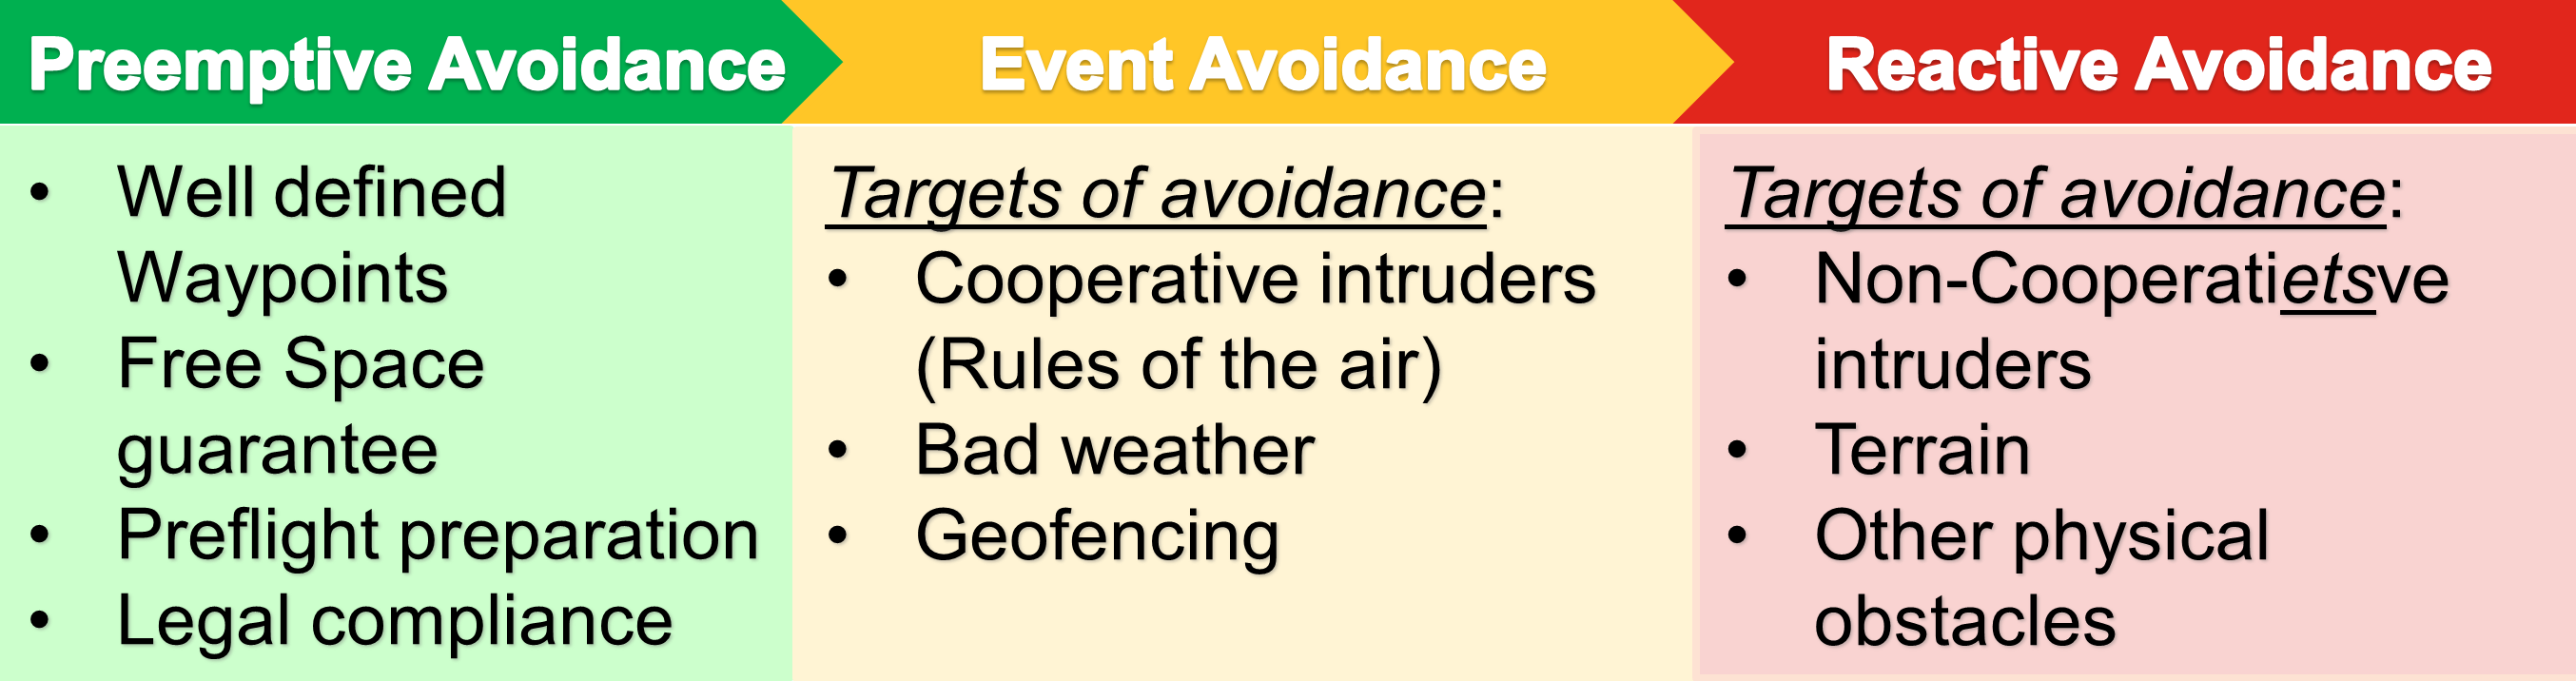
\includegraphics[width=0.7\linewidth]{\FIGDIR/RE001AvoidanceLevelsBasedOnReactionTime} 
    \caption{Avoidance levels based on reaction time.}
    \label{fig:AvoidanceLevels}
\end{figure}

\noindent This work will focus on handling \emph{Event Avoidance}, and \emph{Reactive Avoidance} and the \emph{Avoidance Path} will be calculated using \emph{Reach set Based Methods}. 

The \emph{Preemptive Avoidance} is trying to remove any possible threat before the flight. The risk mitigation is tedious and its done only when necessary. Even the best \emph{preemptive} avoidance could fail.

\emph{Reactive Avoidance} is solving most urgent situations with very short reaction opportunity. This work focus on physical obstacles and terrain. Non-cooperative intruders are partially considered. The adversary behavior was is not considered.

\emph{Event Avoidance} has more opportunity to react. Some threats are known prior the flight (geo-fenced areas, etc.). The future UTM implementation is also considered as \emph{Event Avoidance}, due to the time horizon and authority enforcement. 

\paragraph{Basic Idea:} Create deterministic finite-time \emph{Reactive Avoidance} based on \emph{Reach sets} to ensure \emph{trajectory feasibility}. Enhance method with a set of the rules to enable handling more complex situations.

The \emph{Discretization} is the key to ensure calculation in finite time. Finite \emph{partition} of \emph{operational space (Known World)} and finite representation of \emph{Reach set} guarantees finite count of calculation steps. Aircraft conflict prediction mentioned in \cite{prandini2008application}.

\newpage    
\section{Overview}\label{s:approachOverview}

\noindent The \emph{Overview} is based on \emph{Existing} Emergency avoidance framework \cite{gomola2017obstacle} (fig. \ref{fig:avoidanceConcept}). To achieve goals defined in \emph{Problem Definition} (sec. \ref{s:BasicProblemDefinition}, \ref{s:IncrementalProblemDefinition}) following \emph{Avoidance Framework Concept} (fig. \ref{fig:AvoidanceFrameworkConceptNew}) is proposed:

\begin{figure}[H]
    \centering
    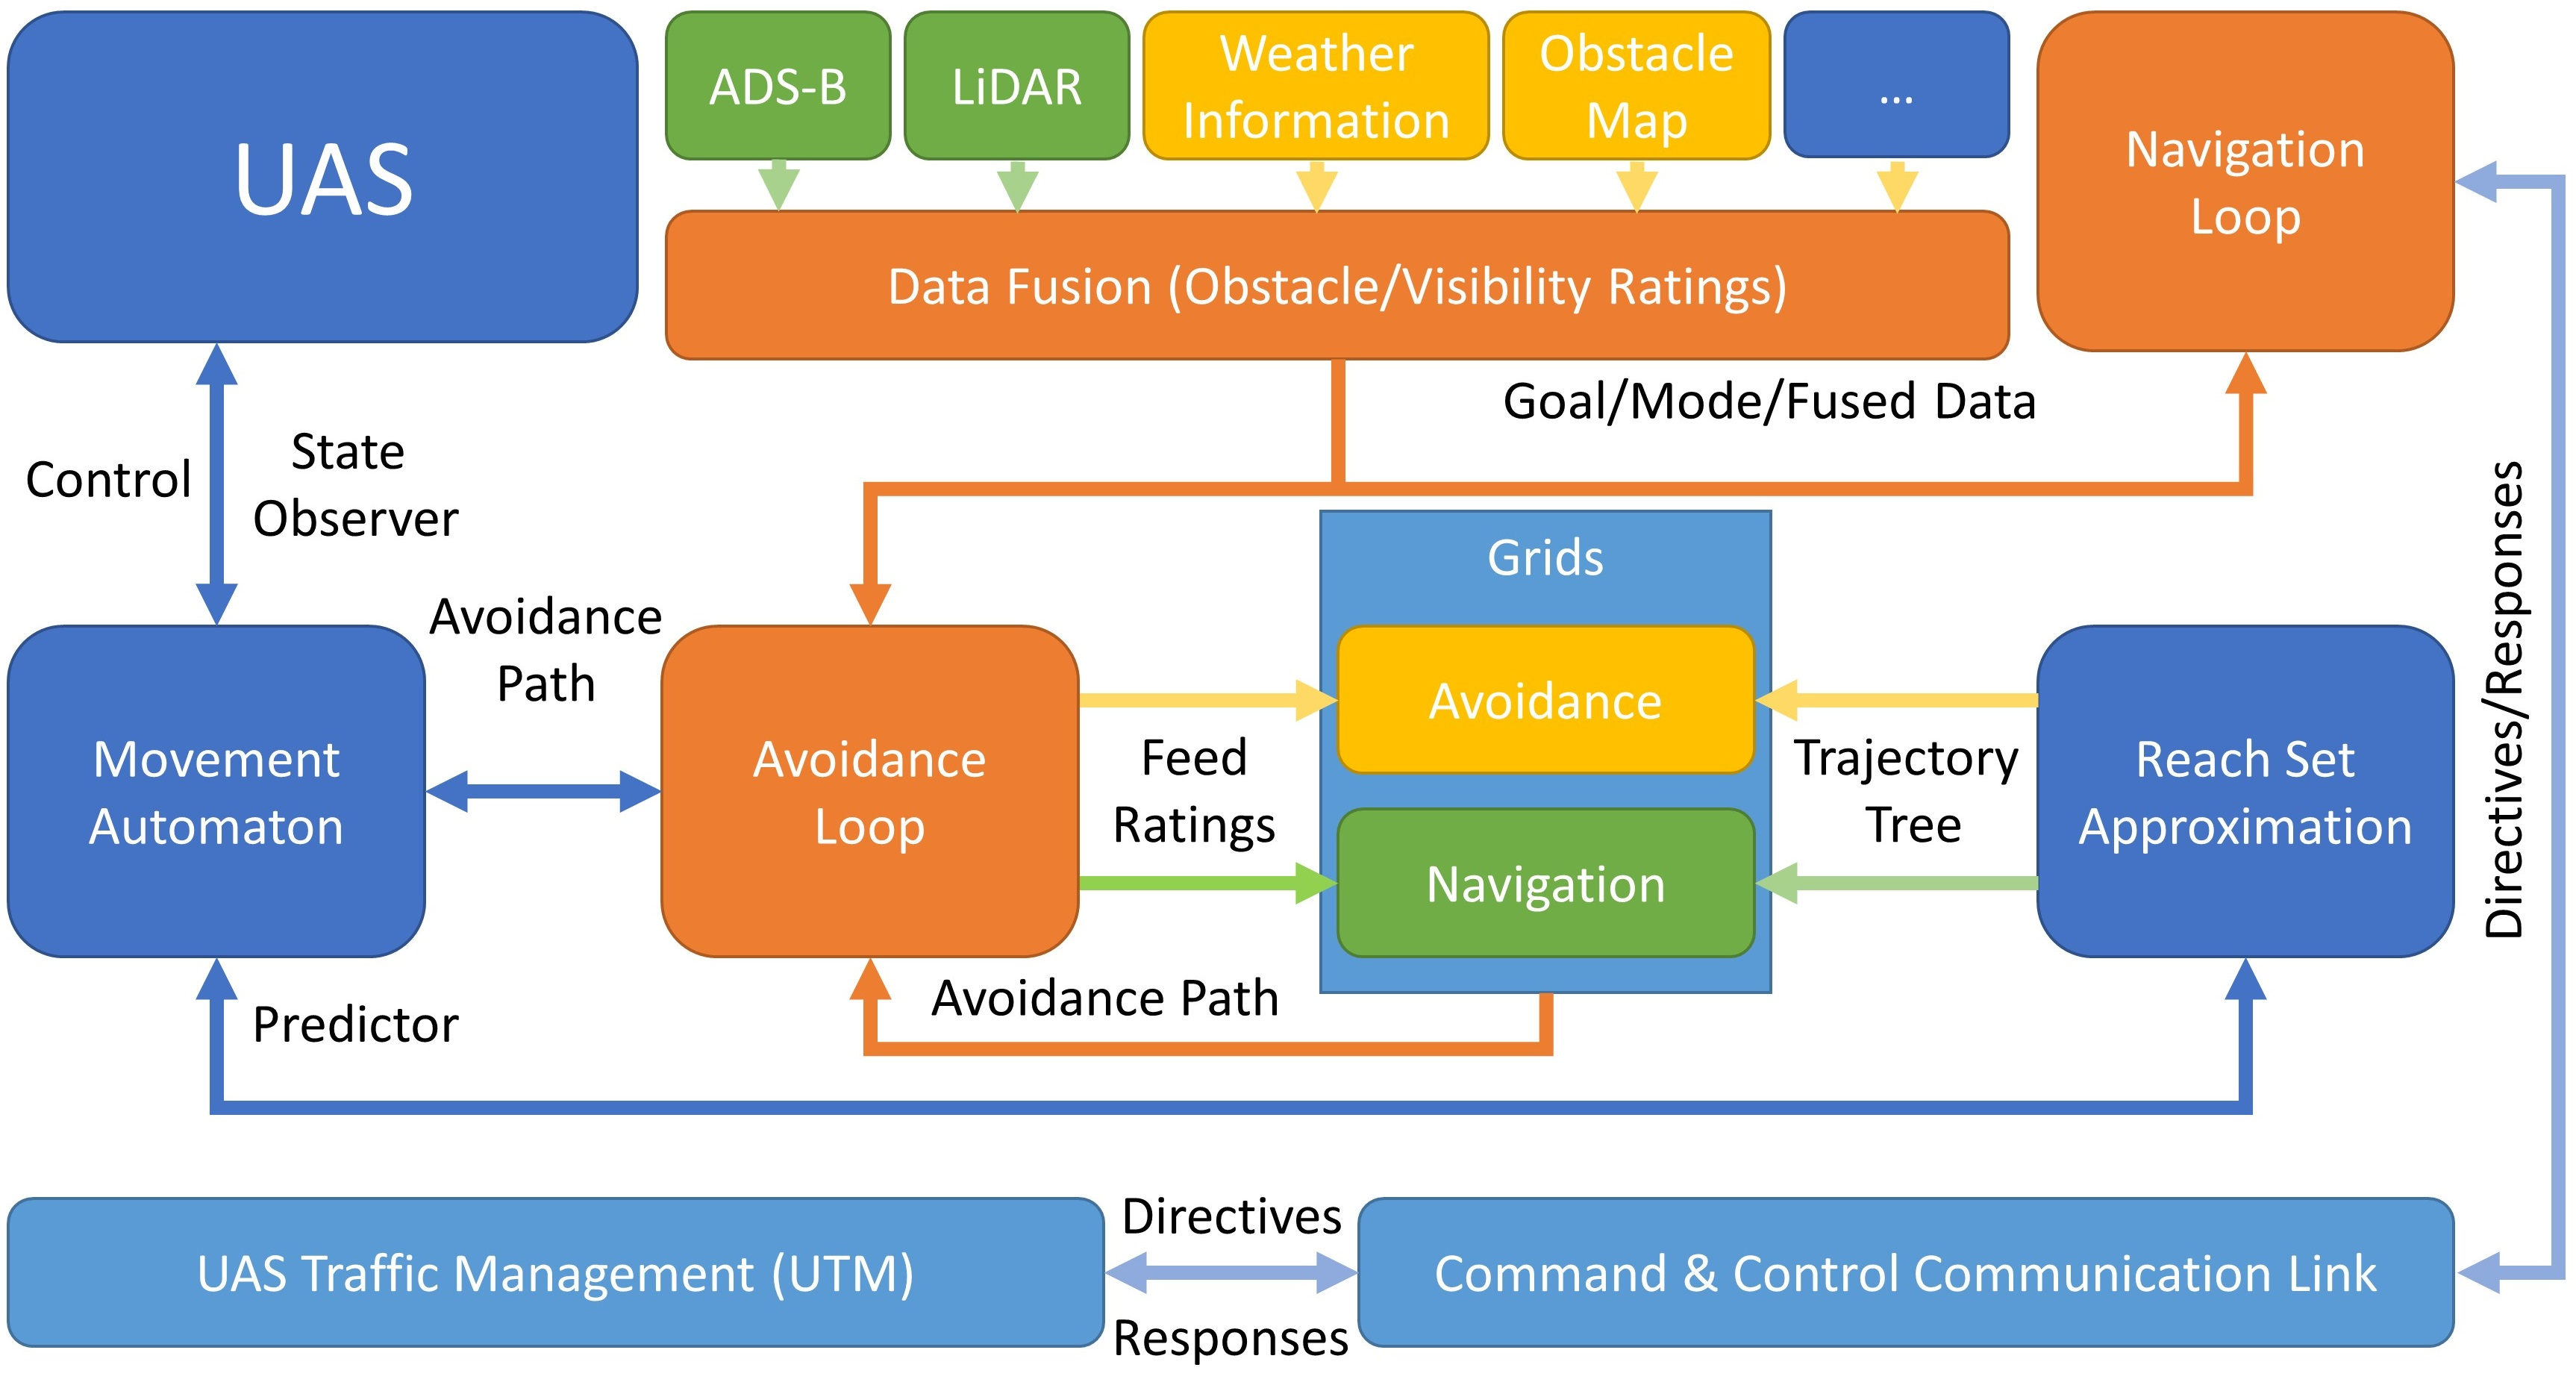
\includegraphics[width=0.95\linewidth]{\FIGDIR/TE037ConceptualSchemeNew} 
    \caption{Avoidance Framework Concept.}
    \label{fig:AvoidanceFrameworkConceptNew}
\end{figure}


\paragraph{Structure of Avoidance Framework:}

\begin{enumerate}
    \item \emph{Unmanned Aircraft System} (UAS) (Role: Controlled Plant) - the \emph{UAS} is controlled via \emph{interface} implemented as \emph{Movement Automaton}. The model used is described in (sec. \ref{s:UASNonlinearModel}).
    
    \item \emph{Movement Automaton} (Role: Control Interface/Predictor) - consumes \emph{Discrete Command Chain} to generate discrete \emph{reference trajectory}, it can  also be used as a predictor of \emph{future UAS states} (sec. \ref{s:referenceTrajectoryGenerator}). The movement Automaton used in this work is given in (sec. \ref{s:movementAutomatonDefinition}). 
    
    \item \emph{Sensor Field} (Role: Surveillance Providers), the following sensors, were considered in this work:
        \begin{enumerate}[a.]
            \item \emph{LiDAR} (Static obstacle detection) - detection of physical obstacles (eq. \ref{eq:naiveObstacleRate})
            
            \item \emph{ADS-B} (Intruder UAS/Plane detection) - detection of intruders who are broadcasting their position and sometimes heading with plans and additional parameters. The \emph{intersection models} are given in (sec. \ref{s:intruders}, app. \ref{s:linearIntersectionModel}, \ref{s:bodyvolumeIntersection}, \ref{s:uncertaintyIntersection}).
        \end{enumerate}
        
    \item \emph{Information Sources} (Role: Known World Information Enhancers): 
        \begin{enumerate}[a.]
            \item \emph{Obstacle Map} (Static Restriction Source) - imposing static soft/hard constraints on \emph{Known Word}/\emph{Operational Space}. Static constraints are given in (sec. \ref{s:virtualConstraints}).
            
            \item \emph{Weather Information} (Static/Dynamic Restriction Source) - imposing static/mo\-vi\-ng soft/hard constraints on \emph{Known World}/\emph{Operational Space}. Moving constraints are given by (def. \ref{def:movingConstraint}).
            
            \item \emph{Other Airspace Restrictions} - like restricted airspace, geo-fencing, and other future constraint sources, all of them are covered by \emph{Static/Dynamic Constraints} for now.
        \end{enumerate}
    
    \item \emph{Data Fusion} (Role: Sensor Input Interface) - is the unifying interface to asses \emph{Operational State Properties} mainly \emph{Obstacle Rating}, \emph{Visibility}, \emph{Map Obstacle Rating}, \emph{Intruder Rating} for a portion of the space. The partial \emph{ratings} are proposed in related sections. The data fusion procedure with \emph{defuzzification} and final assessment into space sets are outlined in (sec. \ref{s:sensorFusion})  
    
    \item \emph{Reach Set Approximation} (Role: Reachability Estimator) - as \emph{data fusion} is providing the situation assessment, the \emph{Reach set} is providing maneuvering capability assessment. The introduction is given in (sec. \ref{s:reachSet}), the properties are defined in (sec. \ref{s:ReachSetPerformanceCriteria}), the approximation methods with constrained expansion are outlined in (sec. \ref{s:chaoticReachSet}, \ref{s:harmonicReachSet}, \ref{s:combinedReachSet}, \ref{s:acasReachSet}). The reach set estimation is the main contribution of this work.
    
    \item \emph{Grids: Navigation/Avoidance} (Role: Operation Space Segmentation \& Situation Evaluation) - space discretization in polar coordinates grid, different reach sets are used for different grid type, defined in (sec. \ref{s:AvoidanceGrid}).
    
    \item \emph{Avoidance loop} (Role: Short Term Decision Maker) - using data from \emph{Sensor fusion} in \emph{Avoidance/Navigation Grid} trimming \emph{Reachable Space} approximated by \emph{Reach Set} generating feasible \emph{Avoidance Path}. \emph{Avoidance Path} is fed to controlling \emph{Movement Automaton}. The Goal is given by \emph{Navigation Loop}. Avoidance loop is given in (sec. \ref{s:aviudabceGridRun}).
    
    \item \emph{Navigation loop} (Role: Long Term Decision Maker) - using data from \emph{Avoidance Loop}, \emph{Mission plan} and \emph{UTM} directives defines the current long term navigation goal. Details are given in (sec. \ref{s:missionControlRun}).
    
    \item \emph{Command and Control Communication Link} (C2 Link) (Role: Communication Link) - standard communication link with sufficient reliability.
    
    \item \emph{UAS Traffic Management} (UTM) (Controlled Airspace Authority) - checking possible collisions and enforces counter-measurements. Details are given in (sec. \ref{sec:UASTrafficManagement}).
    
\end{enumerate}

\paragraph{Communication in Avoidance Framework:}
\begin{enumerate}
    \item \emph{UAS $\leftrightarrow$ Movement Automaton} - sharing \emph{actual system state}, commanding the UAS platform.
    
    \item \emph{Reach Set $\leftrightarrow$ Movement Automaton} - predicting a set of feasible trajectories for the given situation.
    
    \item \emph{Reach Set $\leftrightarrow$ Grids} - providing trajectory set depending on the active mode (Navigation/Emergency Avoidance).
    
    \item \emph{Avoidance Loop $\leftrightarrow$ Data Fusion} - assessing the situation in \emph{operational space} based on sensor readings/information sources.
    
    \item \emph{Avoidance Loop $\leftrightarrow$ Navigation Loop} - determining long term goal based on situation assessment and UTM directives. 
    
    \item \emph{Avoidance Loop $\to$ Grids} - feeding assessment data and constraints into selected operational space Grid.
    
    \item \emph{Grids $\to$ Avoidance Loop} - returning feasible and \emph{cost-effective} avoidance path after situation assessment and \emph{Reach set} pruning.
    
    \item \emph{Avoidance Loop $\to$ Movement Automaton} - issuing and monitoring movement commands based on actual \emph{avoidance strategy}.
    
    \item \emph{Navigation Loop $\leftrightarrow$ C2 Link $\leftrightarrow$ UTM} - communication to receive directives and send fulfillment. 
\end{enumerate}
	
	%06-03 Movement Automaton
    \cleardoublepage
\section{\secState{R}UAS Model and Control}\label{s:modelMAImplementation}

\noindent The key feature of \emph{Movement Automaton} is to interface \emph{continuous-control signal} as the \emph{discrete command chain}. Following topics are introduced in this section:

\begin{enumerate}
    \item \emph{UAS Nonlinear Model} (sec. \ref{s:UASNonlinearModel}) - simple plane model used in this work as \emph{controlled plant}.
    
    \item \emph{Movement Automaton} (sec. \ref{s:movementAutomatonDefinition}) - movement automaton for \emph{UAS Nonlinear Model} constructed from scratch.
    
    \item \emph{Segmented Movement Automaton} (sec. \ref{s:segmentedMovementAutomaton}) - for more complex systems the \emph{State Space} can be \emph{separated into Segments} and \emph{segment movement automaton} is used to generate \emph{thick reference trajectory}.
    
    \item \emph{Reference Trajectory Generator} (sec. \ref{s:referenceTrajectoryGenerator}) - other use of \emph{Movement Automaton} as predictor for \emph{reference trajectory calculation}.
\end{enumerate}


\subsection{\secState{R}UAS Nonlinear Model}\label{s:UASNonlinearModel}
\paragraph{Motivation:} Simplified rigid body kinematic model will be used. This model have decoupled roll, yaw and pitch angles. The focus is on \emph{reach set approximation methods}, therefore \emph{UAS model} is simplified.

\paragraph{State Vector} (eq. \ref{eq:simple3dStatevector}) defined as positional state in euclidean position in right-hand euclidean space, where \emph{x, y, z} can be abstracted as latitude, longitude, altitude.
\begin{equation}\label{eq:simple3dStatevector}
    state = \left [ x,y,z, roll, pitch, yaw \right]^T
\end{equation}


\paragraph{Input Vector} (eq. \ref{eq:simple3dInputVector}) is defined as linear velocity of UAS $v$ and angular speed of rigid body $\omega_{roll}, \omega_{pitch},\omega_{yaw}$.

\begin{equation}\label{eq:simple3dInputVector}
    input = \left [ v, \omega_{roll}, \omega_{pitch},\omega_{yaw}\right ]^T
\end{equation}


\noindent Velocity distribution function (eq. \ref{eq:simple3dvelocityDistribution})  is is defined trough standard rotation matrix  and linear velocity $v$, oriented velocity [$v_x$, $v_y$, $v_z$] given by (eq. \ref{eq:UASNonlinearModelSimple}).

\begin{equation}\label{eq:simple3dvelocityDistribution}
    \begin{bmatrix}
    v_x\\
    v_y\\
    v_z\
    \end{bmatrix}
    =
    \begin{bmatrix}
         v\cos(pitch)\cos(yaw)\\
         v\cos(pitch)\sin(yaw)\\
         -v\sin(pitch)\\
    \end{bmatrix}
\end{equation}

\paragraph{UAS Nonlinear Model} (eq. \ref{eq:UASNonlinearModelSimple}) is given by \emph{first order equations:}

\begin{equation}\label{eq:UASNonlinearModelSimple}
    \begin{aligned}
        \frac{\partial x}{\partial time} &= v\cos(pitch)\cos(yaw);\\
        \frac{\partial y}{\partial time} &= v\cos(pitch)\sin(yaw);\\
        \frac{\partial z}{\partial time} &= -v\sin(pitch);\\
    \end{aligned}\\\quad\quad
    \begin{aligned}
        \frac{\partial roll}{\partial time} &= \omega_{roll};\\
        \frac{\partial pitch}{\partial time} &= \omega_{pitch};\\
        \frac{\partial yaw}{\partial time} &= \omega_{yaw};\\
    \end{aligned}
\end{equation}

\subsection{\secState{R}Movement Automaton for UAS Model}\label{s:movementAutomatonDefinition}

\paragraph{Motivation:} An \emph{UAS Nonlinear Model} (eq. \ref{eq:UASNonlinearModelSimple}) can be modeled by \emph{Movement Automaton} (def. \ref{def:movementAutomaton}). 

\paragraph{Movement Primitives} by (def. \ref{def:MovementPrimitive})  are given as (eq. \ref{eq:movementPrimitive}). To define primitives the \emph{minimal time} is $1 s$. The \emph{maximal duration} is also $1s$. 

\begin{assumption}\label{ass:transitionTime}
    Let assume that \emph{transition time} of \emph{roll, pitch, yaw, linear velocity} is $0 s$.
\end{assumption}

Under the assumption (as. \ref{ass:transitionTime}) the \emph{movement transitions} (def. \ref{def:movementTransition}) have $0$ duration.

\begin{note}
    The assumption (as. \ref{ass:transitionTime}) can be relaxed under condition that \emph{path tracking controller exists}.
\end{note}

\paragraph{Movements} (def. \ref{def:Movement}) for \emph{fixed step} $k$ we start with discretization of the input variables.

\noindent The \emph{linear velocity} in text step is given:
\begin{equation}\label{eq:applyMovement}
    v(k+1) = v(k) +\delta v(k)
\end{equation}

\noindent The \emph{roll, pitch, yaw} for next step are given 

\begin{equation}\label{eq:applyMovement1}
    \begin{aligned}
        roll(k+1)  &= roll(k) + \delta roll(k)\\
        pitch(k+1) & = pitch(k) + \delta pitch(k)\\
        yaw(k+1) & = yaw(k) + \delta yaw(k)\\
    \end{aligned}    
\end{equation}

\noindent The $\delta v(k)$ is \emph{velocity change}, $\delta roll(k)$, $\delta pitch(k)$, $\delta yaw(k)$, are \emph{orientation changes} for current discrete step $k$. If the duration of \emph{transition} is $0 s$ (as. \ref{ass:transitionTime}) then 3D trajectory evolution in discrete time is given as: 

\begin{equation}\label{eq:applyMovement2}
    \begin{aligned}
        x(k+1)&= x(k) + v(k+1) \cos(pitch(k+1)) \cos(yaw(k+1)) & = \delta x(k)\\
        y(k+1)&= y(k) + v(k+1) \cos(pitch(k+1)) \sin(yaw(k+1)) & = \delta y(k)\\
        z(k+1)&= z(k) - v(k+1) \sin(pitch(k+1))                & = \delta z(k)\\
        time(k+1)& = time(k)+1                                & = \delta time(k)
    \end{aligned}    
\end{equation}

\noindent The $\delta x(k)$, $\delta y(k)$, $\delta z(k)$ are positional differences depending on \emph{input vector} for given discrete time $k$:
\begin{equation}\label{eq:ourImput}
    input(k) = \left[
                    \begin{gathered}
                    \delta x(k), \delta y(k), \delta z(k), \delta v (k),\\
                    \delta roll (k), \delta pitch(k), \delta yaw(k),\delta time (k)
                    \end{gathered} 
                \right]^T
\end{equation}

\noindent The \emph{state vector} for discrete time is given:
\begin{equation}\label{eq:ourState}
    state(k) = \left[
                    \begin{gathered}
                     x(k),  y(k),  z(k),  v (k),\\
                     roll (k),  pitch(k),  yaw(k), time (k)
                    \end{gathered} 
                \right]^T
\end{equation}

\noindent The nonlinear model (eq. \ref{eq:UASNonlinearModelSimple}) is then reduced to \emph{linear discrete model} (eq. \ref{eq:uasLinearDiscreteModel}) given by \emph{apply movements} function (eq. \ref{eq:applyMovement}, \ref{eq:applyMovement1}, \ref{eq:applyMovement2}).

\begin{equation}\label{eq:uasLinearDiscreteModel}
    state(k+1) = applyMovement(state(k), input(k)) 
\end{equation}

\paragraph{Movement Set} for linear discrete model (eq. \ref{eq:uasLinearDiscreteModel}) is defined as set of extreme unitary movements on main axes (tab. \ref{tab:movements1}) and diagonal axes (tab. \ref{tab:movements2}).

\begin{table}[H]
    \centering
    \begin{tabular}{r||r|r|r|r|r}
    
        $input(movement)$           &    Straight  & Down & Up & Left  & Right   \\\hline\hline
        $\delta     x(k)[m]$           &    1.00	  & 0.98  & 0.98  & 0.98 & 0.98  \\\hline
        $\delta     y(k)[m]$           &    0	      & 0	  & 0	  & 0.13 & -0.13 \\\hline
        $\delta     z(k)[m]$           &    0	      & -0.13 & 0.13  &	0	 & 0     \\\hline
        $\delta  roll(k) [^\circ]$	   &    0	      & 0	  & 0	  & 0    & 0     \\\hline
        $\delta pitch(k) [^\circ]$     &    0	      & $15^\circ$  & -$15^\circ$ & 0	 & 0     \\\hline
        $\delta   yaw(k) [^\circ]$     &    0	      & 0	  & 0	  & $15^\circ$ & -$15^\circ$ \\
    \end{tabular}
    \caption{Input values for main axes movements.}
    \label{tab:movements1}
\end{table}
\begin{table}[H]
    \centering
    \begin{tabular}{r||r|r|r|r}
        $input(movement)$             & Down-Left & Down-Right & Up-Left  & Up-Right   \\\hline\hline
        $\delta     x(k)[m]$           & 0.76  & 0.76  & 0.76 & 0.76  \\\hline
        $\delta     y(k)[m]$           & -0.13	& 0.13	& 0.13 & -0.13 \\\hline
        $\delta     z(k)[m]$           & -0.13 & -0.13 & 0.13 & 0.13  \\\hline
        $\delta  roll(k) [^\circ]$	& 0	    & 0	    & 0    & 0     \\\hline
        $\delta pitch(k) [^\circ]$     & -$15^\circ$ & -$15^\circ$ & $15^\circ$ & $15^\circ$     \\\hline
        $\delta   yaw(k) [^\circ]$    & $15^\circ$	& -$15^\circ$	& $15^\circ$ & -$15^\circ$ \\
    \end{tabular}
    \caption{Input values for diagonal axes movements.}
    \label{tab:movements2}
\end{table}

\begin{note}
    \emph{Movement set} in shorten form is given as
    \begin{equation}\label{eq:OurMovementSet}
        Movement Set= \left\{
        \begin{gathered}
            Straight, Left,Right, Up, Down,\\
            Down Left, Down Right,  Up Left,   Up Right
        \end{gathered}
        \right\}
    \end{equation}
\end{note}

\paragraph{Trajectory} by (def. \ref{def:MovementAutomatonTrajectory}) for initial time $time = 0$ , initial state $state(0)$ and \emph{Movement Buffer} (from def. \ref{def:MovementBuffer}):
\begin{equation}\label{eq:ourBuffer}
    Buffer \in Movement Set^* (eq. \ref{eq:OurMovementSet}), \quad  |Buffer| \in \N
\end{equation}

\noindent Trajectory (eq. \ref{eq:ourTrajectoryImplementation}) is then given as the time-series of discrete states:
\begin{equation}\label{eq:ourTrajectoryImplementation}
    Trajectory(state(0),Buffer)= \left\{\begin{gathered}state(0)+\sum_{j=0}^{i-1} input(movement(j)):\\i \in\left\{1\dots |Buffer|+1\right\}, \\movement(\cdot) \in Buffer\end{gathered}\right\}
\end{equation}

\noindent Trajectory (eq. \ref{eq:ourTrajectoryImplementation}) is ordered set of states bounded to discrete time $0\dots n$ , where $n$ is member count of \emph{Buffer}. Trajectory set has $n+1$ members:

\begin{equation}
    \begin{aligned}
    T&rajectory(state(0),Buffer)=\\
        &\left\{
        \begin{aligned}
            state(0) &= state(0) + \{\}\\
            state(1) &= state(0) + input(movement(1))\\
            state(2) &= state(0) + input(movement(1)) +input(movement(2))\\
             \vdots  &= \vdots\\
            state(n) &= state(0) + input(movement(1))+\dots+input(movement(n))\\
        \end{aligned}
        \right\}
    \end{aligned}
\end{equation}

\paragraph{State Projection} (eq. \ref{eq:ourStateProjection}) for the \emph{Trajectory} (eq. \ref{eq:ourTrajectoryImplementation}) is given as follow:
\begin{equation}\label{eq:ourStateProjection}
    StateProjection(Trajectory,time) = Trajectory.getMemberByIndex(time+1)
\end{equation}

\begin{note}
    \emph{Movement Automaton} for system (eq. \ref{eq:UASNonlinearModelSimple}) with given (as. \ref{ass:transitionTime}) is established with all related properties (sec. \ref{def:movementAutomaton}).
\end{note}

\newpage
\subsection{\secState{R}Segmented Movement Automaton}\label{s:segmentedMovementAutomaton}
\paragraph{Motivation:} Constructing \emph{Movement Automaton} for more complex system can be tedious. Used \emph{Movement Automaton} for \emph{UAS system} (\ref{eq:UASNonlinearModelSimple}) has decoupled control which is not true for most of the copters/planes \cite{fossen2011mathematical}.

\paragraph{Partitioning UAS State Space:} Proposed movement automaton is defined by its Movement set (tab. \ref{tab:movements1},\ref{tab:movements2}). Those can be scaled depending on maneuverability in the  \emph{Initial state} $state(0)$:
\begin{enumerate}
    \item \emph{Climb/Descent Rate} $\delta pitch_{max}(k)$ - the maximal climb or descent rate for Up/Down movements.
    \item \emph{Turn Rate} $\delta yaw_{max}(k)$ - the maximal turn rate for Left/Right movement.
    \item \emph{Acceleration} $\delta v_{max}(k)$ - the maximal acceleration in cruising speed range.
\end{enumerate}

\begin{definition}{State Space partition}\label{def:stateSpacePartition}
    \emph{Maneuverability} is depending on \emph{Initial State}. There can not be the infinite count of \emph{Movement Automatons}.
    
    The state space $State Space \in \R^n$ can be separated into two exclusive subsets:
    \begin{equation}
        StateSpace = [ImpactStates, NonImpactingStates]
    \end{equation}
    
    The \emph{Impacting states} are states which bounds the \emph{Maneuverability}: $\delta pitch_{max}(k)$, $\delta yaw_{max}(k)$, $\delta v_{max}(k)$. For each \emph{impact state} is possible to define upper and lower boundary:
    \begin{multline}
        \forall impactState\in ImpactStates, \exists:\\ lower(impactState) \le value(impactState) \le upper(impactState) 
    \end{multline}
    
	\noindent    The bounded interval of impact state can be separated into distinctive \emph{impact state segments} like follow:
    \begin{multline}
        impactState\in [lower,upper]:\\ \{[lower,separator_1[\dots\cup\dots[separator_i,separator_{i+1}[\dots\cup\dots\\\dots\cup\dots[separator_n,upper]\}=\\
        = impactStateIntervals(impactState)
    \end{multline}
    \begin{note}
        The interval length depends on model dynamics. The rule of thumb is to keep maximal climb/descend/turn/acceleration rates near constant value. 
    \end{note}
        
\noindent When partitioning of \emph{all impact States} finishes, the count of partitions is given as product of \emph{count of partitions} for each member of \emph{Impact States}:
    
    \begin{equation}
        partition Count = \prod_{impactState \in}^{ImpactStates} |impactStateIntervals(impactState)| 
    \end{equation}
    
    \begin{note}
        Try to keep the count of partitions to minimum, each new interval increases the count of partitions geometrically. 
    \end{note}
    
    There is finite number $n$ of \emph{Impacting States}, these are separated into $impactState-$ $Intervals_i$ with respective index $i \in 1\dots n$. The \emph{segment} with index defining position used \emph{impacting state} intervals is given as \emph{constrained space}:
    
    \begin{equation}
        Segment(index) = \left[
            \begin{gathered}
                impactState_1 \in impactStateIntervals_1[index_1],\\
                \vdots\\
                impactState_n \in impactStateIntervals_n[index_n],\\
                \vdots\\
                NonImpactingStates    
                \end{gathered}\right]
    \end{equation}
    
    Each \emph{Segment} covers one of impacting state intervals combination, because the original intervals are exclusive, also \emph{Segments} are exclusive. The \emph{union} of all segments covers \emph{State Space}:
    
    \begin{equation}\label{eq:segmentedStateSpace}
        StateSpace = \bigcup_{\forall\quad index \in |impactStateIntervals|^n} Segment(index)
    \end{equation}
\end{definition}

\paragraph{Segmented Movement Automaton:} The segmentation of \emph{state space} is done  in (def. \ref{def:stateSpacePartition}) any \emph{state} belongs exactly to \emph{Segment} of \emph{State Space}. For each \emph{Segment} in \emph{State Space}it is possible to assess: \emph{Climb/Descent Rate} $\delta pitch_{max}(k)$, \emph{Turn Rate} $\delta yaw_{max}(k)$, and, \emph{Acceleration} $\delta v_{max}(k)$.


\begin{definition}{Movement Automaton for Segment(index)}\label{def:segmentMovementAutomaton}
    

\noindent For for Model(eq. \ref{eq:uasLinearDiscreteModel}) with State (eq. \ref{eq:ourState}) the input vector (eq. \ref{eq:ourImput}) is for position $[x,y,z]$ and velocity defined like: 

\begin{equation}
    \begin{aligned}
        \delta x(k)& = \left(v(k)+\delta v(k)\right) \cos(\delta pitch(k)) \cos(\delta yaw(k))\\
        \delta y(k)& = \left(v(k)+\delta v(k)\right) \cos(\delta pitch(k)) \sin(\delta yaw(k))\\
        \delta z(k)& = -\left(v(k)+\delta v(k)\right)\cos(\delta pitch(k))\\
        \delta v(k)&\in [-\delta v(k)_{max},\delta v(k)_{max}]
    \end{aligned}
\end{equation}
\end{definition}

\noindent The acceleration $\delta v(k)$ is in interval $[-\delta v(k)_{max},\delta v(k)_{max}]$, usually set to 0 $ms^{-1}$. The change of the orientation angles for \emph{Movement Set} (eq. \ref{eq:OurMovementSet}) is given in (tab. \ref{tab:movements3},\ref{tab:movements4}).

\begin{table}[H]
    \centering
    \begin{tabular}{r||r|r|r|r|r}
    
        $input(movement)$           &    Straight  & Down & Up & Left  & Right   \\\hline\hline
        $\delta  roll(k) [^\circ]$	   &    0	      & 0	  & 0	  & 0    & 0     \\\hline
        $\delta pitch(k) [^\circ]$     &    0	      & $\delta pitch_{max}$  & -$\delta pitch_{max}$ & 0	 & 0     \\\hline
        $\delta   yaw(k) [^\circ]$     &    0	      & 0	  & 0	  & $\delta yaw_{max}$ & -$\delta yaw_{max}$ \\
    \end{tabular}
    \caption{Orientation input values for main axes movements.}
    \label{tab:movements3}
\end{table}


\begin{table}[H]
    \centering
    \begin{tabular}{r||r|r|r|r}
        $input(movement)$             & Down-Left & Down-Right & Up-Left  & Up-Right   \\\hline\hline

        $\delta  roll(k) [^\circ]$	& 0	    & 0	    & 0    & 0     \\\hline
        $\delta pitch(k) [^\circ]$     & -$\delta pitch_{max}$ & -$\delta pitch_{max}$ & $\delta pitch_{max}$ & $\delta pitch_{max}$     \\\hline
        $\delta   yaw(k) [^\circ]$    & $\delta yaw_{max}$	& -$\delta yaw_{max}$	& $\delta yaw_{max}$ & -$\delta yaw_{max}$ \\
    \end{tabular}
    \caption{Orientation input values for diagonal axes movements.}
    \label{tab:movements4}
\end{table}

\begin{note}
    The \emph{Trajectory} is calculated same as in (eq. \ref{eq:ourTrajectoryImplementation}). The \emph{State Projection} is given as in (eq. \ref{eq:ourStateProjection}).
\end{note}

\noindent Then the \emph{Movement Automaton} for \emph{Segment} $\in$ \emph{State Space} is defined.

\begin{definition}{Segmented Movement Automaton}\label{def:segmentedMovementAutomaton}
    For system with segmented state space (eq. \ref{eq:segmentedStateSpace}) there is for each $state(k)$ in $StateSpace$ injection function:
    \begin{equation} \label{eq:activeMovementAutomaton}
        ActiveMovementAutomaton:StateSpace\to MovementAutomaton
    \end{equation}
    
\noindent Selecting appropriate \emph{movement automaton} implementation (def. \ref{def:segmentMovementAutomaton}) for \emph{state(k)} $\in$ \emph{Segment} $\subset$ \emph{State Space}. The mapping function (eq. \ref{eq:activeMovementAutomaton}) is injection mapping every state(k) to Segment then \emph{Movement Automaton Implementation}. The trajectory generated is then given:
    
    \begin{equation}\label{eq:ourTrajectoryImplementationSegmented}
        Trajectory\left(\begin{gathered}state(0),\\Buffer\end{gathered}\right)= 
        \left\{
            \begin{gathered}
                state(0)+\dots\\\sum_{j=0}^{i-1} 
                    \begin{aligned} 
                        &ActiveMovementAutomaton(state(j-1)).\\
                        &\quad.input(movement(j))
                    \end{aligned}:\\
                i \in\left\{1\dots |Buffer|+1\right\}, \\
                movement(\cdot) \in Buffer
            \end{gathered}
        \right\}
    \end{equation}
    
\end{definition}

\newpage
\subsection{\secState{R}Reference Trajectory Generator}\label{s:referenceTrajectoryGenerator}

\paragraph{Reference Trajectory Generator:} Segmented Movement Automaton (def.  \ref{def:segmentedMovementAutomaton}) with \emph{trajectory function} (eq. \ref{eq:ourTrajectoryImplementationSegmented}) is used as \emph{reference trajectory generator} for \emph{complex systems}. 

There is assumption that precise \emph{path tracking} implementation exist for such system which with \emph{thick reference trajectory} gives similar results to \emph{plain movement automaton control}.

The \emph{Reference trajectory} (eq. \ref{eq:generatedReferenceTrajectory}) for \emph{Planned} movement set is given as projection  of \emph{Trajectory} time series to position time series $[x,y,z,t]$:

\begin{equation}\label{eq:generatedReferenceTrajectory}
    Reference Trajectory:Trajectory\left(\begin{gathered}state(now),\\Planned\end{gathered}\right) 
    \to 
    \begin{bmatrix}
        x_{ref} \in \R^{|Planned|}\\
        y_{ref} \in \R^{|Planned|}\\
        z_{ref} \in \R^{|Planned|}\\
        t_{ref} \in \R^{|Planned|}
    \end{bmatrix}
\end{equation}

\paragraph{Predictor:} The \emph{Reference Trajectory Generator} (eq. \ref{eq:generatedReferenceTrajectory}) can be also used as predictor. 

\begin{note}
    The \emph{Segmented Movement Automaton} (def. \ref{def:segmentedMovementAutomaton}) is used in this work with one Segment equal to State space with input function given by (\ref{tab:movements1}, \ref{tab:movements2}). The predictor used in \emph{Reach set computation} is given by (eq. \ref{eq:generatedReferenceTrajectory}).
\end{note}

    	\subsection{\secState{R}Movement Automaton Applications}\label{sec:MovementAutomatonBackground}

    \noindent\emph{Movement Automaton} is basic interface approach for discretization of \emph{trajectory evolution}  or \emph{control input} for any \emph{continuous or discrete system model}.
    
    \emph{Main function} of \emph{Movement Automaton is} for system given by equation $\dot{state}=f(time,state,input)$ with initial state $state_0$ to generate \emph{reference trajectory} $\hat{state}(t)$ or \emph{control signal} $input(t)$.
    
    Using \emph{Movement Automaton} as \emph{Control Proxy} will provide us with \emph{discrete command chain} interface. This will reduce the \emph{non deterministic} element from \emph{Evasive trajectory} generation, by reducing infinite maneuver set to finite \emph{movement set}.
    
    \emph{Non determinism} of \emph{Avoidance Maneuver} have been discussed as an issue in following works:
    \begin{enumerate}
        \item Newton gradient method for evasive car maneuvers \cite{vsantin2011combined}.
        \item Non-holistic methods for trajectory generation \cite{pin1990autonomous}.
        \item Stochastic approach to elliptic trajectories generation \cite{andrzejak2001epileptic}.
    \end{enumerate}
    
\noindent\emph{Examples} of \emph{Movement Automaton Implementation} as \emph{Control Element} can be mentioned as follows:
    \begin{enumerate}
        \item Control of traffic flow \cite{kuwata2009real}.
        \item Complex air traffic collision situation resolution system  \cite{frazzoli2001robust,frazzoli2000trajectory}.
        \item SAA/DAA capable avoidance system \cite{gomola2017obstacle}.
    \end{enumerate}



		\subsection{\secState{R}UAS Model}\label{s:UASNonlinearModel}
\paragraph{Motivation:} Simplified rigid body kinematic model will be used. This model have decoupled roll, yaw and pitch angles. The focus is on \emph{reach set approximation methods}, therefore \emph{UAS model} is simplified.

\paragraph{State Vector} (eq. \ref{eq:simple3dStatevector}) defined as positional state in euclidean position in right-hand euclidean space, where \emph{x, y, z} can be abstracted as latitude, longitude, altitude.
\begin{equation}\label{eq:simple3dStatevector}
    state = \left [ x,y,z, roll, pitch, yaw \right]^T
\end{equation}


\paragraph{Input Vector} (eq. \ref{eq:simple3dInputVector}) is defined as linear velocity of UAS $v$ and angular speed of rigid body $\omega_{roll}, \omega_{pitch},\omega_{yaw}$.

\begin{equation}\label{eq:simple3dInputVector}
    input = \left [ v, \omega_{roll}, \omega_{pitch},\omega_{yaw}\right ]^T
\end{equation}


\noindent Velocity vector function (eq. \ref{eq:simple3dvelocityDistribution})  is is defined through standard rotation matrix  and linear velocity $v$, oriented velocity [$v_x$, $v_y$, $v_z$] given by (eq. \ref{eq:UASNonlinearModelSimple}).

\begin{equation}\label{eq:simple3dvelocityDistribution}
    \begin{bmatrix}
    v_x\\
    v_y\\
    v_z\
    \end{bmatrix}
    =
    \begin{bmatrix}
         v\cos(pitch)\cos(yaw)\\
         v\cos(pitch)\sin(yaw)\\
         -v\sin(pitch)\\
    \end{bmatrix}
\end{equation}

\paragraph{UAS Nonlinear Model} (eq. \ref{eq:UASNonlinearModelSimple}) is given by \emph{first order equations:}

\begin{equation}\label{eq:UASNonlinearModelSimple}
    \begin{aligned}
        \frac{\text{d} x}{\text{d} time} &= v\cos(pitch)\cos(yaw);\\
        \frac{\text{d} y}{\text{d} time} &= v\cos(pitch)\sin(yaw);\\
        \frac{\text{d} z}{\text{d} time} &= -v\sin(pitch);\\
    \end{aligned}\\\quad\quad
    \begin{aligned}
        \frac{\text{d} roll}{\text{d} time} &= \omega_{roll};\\
        \frac{\text{d} pitch}{\text{d} time} &= \omega_{pitch};\\
        \frac{\text{d} yaw}{\text{d} time} &= \omega_{yaw};\\
    \end{aligned}
\end{equation}

\paragraph{Discretization} for \emph{fixed step} $k$ we start with discretization of the input variables:

\noindent The \emph{linear velocity} in text step is given:
\begin{equation}\label{eq:applyMovement}
    v(k+1) = v(k) +\delta v(k)
\end{equation}

\noindent The \emph{roll, pitch, yaw} for next step are given 

\begin{equation}\label{eq:applyMovement1}
    \begin{aligned}
        roll(k+1)  &= roll(k) + \delta roll(k)\\
        pitch(k+1) & = pitch(k) + \delta pitch(k)\\
        yaw(k+1) & = yaw(k) + \delta yaw(k)\\
    \end{aligned}    
\end{equation}

\noindent The $\delta v(k)$ is \emph{velocity change}, $\delta roll(k)$, $\delta pitch(k)$, $\delta yaw(k)$, are \emph{orientation changes} for current discrete step $k$. If the duration of \emph{transition} is $0 s$ (as. \ref{ass:transitionTime}) then 3D trajectory evolution in discrete time is given as: 

\begin{equation}\label{eq:applyMovement2}
    \begin{aligned}
        x(k+1)&= x(k) + v(k+1) \cos(pitch(k+1)) \cos(yaw(k+1)) & = \delta x(k)\\
        y(k+1)&= y(k) + v(k+1) \cos(pitch(k+1)) \sin(yaw(k+1)) & = \delta y(k)\\
        z(k+1)&= z(k) - v(k+1) \sin(pitch(k+1))                & = \delta z(k)\\
        time(k+1)& = time(k)+1                                & = \delta time(k)
    \end{aligned}    
\end{equation}

\noindent The $\delta x(k)$, $\delta y(k)$, $\delta z(k)$ are positional differences depending on \emph{input vector} for given discrete time $k$:
\begin{equation}\label{eq:ourImput}
    input(k) = \left[
                    \begin{gathered}
                    \delta x(k), \delta y(k), \delta z(k), \delta v (k),\\
                    \delta roll (k), \delta pitch(k), \delta yaw(k),\delta time (k)
                    \end{gathered} 
                \right]^T
\end{equation}

\noindent The \emph{state vector} for discrete time is given:
\begin{equation}\label{eq:ourState}
    state(k) = \left[
                    \begin{gathered}
                     x(k),  y(k),  z(k),  v (k),\\
                     roll (k),  pitch(k),  yaw(k), time (k)
                    \end{gathered} 
                \right]^T
\end{equation}


		\subsection{\secState{R}UAS Movement Automaton}\label{s:movementAutomatonDefinition}

\paragraph{Motivation:} An \emph{UAS Nonlinear Model} (eq. \ref{eq:UASNonlinearModelSimple}) can be modeled by \emph{Movement Automaton} (def. \ref{def:movementAutomaton}). 

\paragraph{Movement Primitives} by (def. \ref{def:MovementPrimitive})  are given as (eq. \ref{eq:movementPrimitive}). To define primitives the \emph{minimal time} is $1 s$. The \emph{maximal duration} is also $1s$.

\begin{note}
	Each movement primitive will last for fixed duration $1s$.
\end{note} 

\begin{assumption}\label{ass:transitionTime}
    Let assume that \emph{transition time} of \emph{roll, pitch, yaw, linear velocity} is $0 s$.
\end{assumption}

Under the assumption (as. \ref{ass:transitionTime}) the \emph{movement transitions} (def. \ref{def:movementTransition}) have zero duration. Therefore movement primitives can be considered as movements.

\begin{note}
    The assumption (as. \ref{ass:transitionTime}) can be relaxed under condition that \emph{path tracking controller exists}.
\end{note}

\paragraph{Movements} satisfying (def. \ref{def:Movement}), for the nonlinear model (eq. \ref{eq:UASNonlinearModelSimple}) reduced to \emph{discrete model} (eq. \ref{eq:uasLinearDiscreteModel}), are given by \emph{apply movements} function (eq. \ref{eq:applyMovement}, \ref{eq:applyMovement1}, \ref{eq:applyMovement2}).

\begin{equation}\label{eq:uasLinearDiscreteModel}
    state(k+1) = applyMovement(state(k), input(k)) 
\end{equation}

\paragraph{Movement Set} for discrete model (eq. \ref{eq:uasLinearDiscreteModel}) is defined as set of unitary movements on main axes (tab. \ref{tab:movements1}) and diagonal axes (tab. \ref{tab:movements2}). 

The maneuvering capability of several commercial small fixed wing UAS were merged together. The turning rate on horizontal/vertical is defined as $15^\circ$.

The deltas are posed in \emph{UAS body-fixed coordinate frame} (ap. \ref{sec:complementsOfAlgebra}) for discrete time $k$. 

\begin{table}[H]
    \centering
    \begin{tabular}{r||r|r|r|r|r}
    	\multirow{2}{*}{Parameter} & \multicolumn{5}{c}{Movement} \\\cline{2-6} 
                &    Straight  & Down & Up & Left  & Right   \\\hline\hline
        $\delta     x(k)[m]$           &    1.00	  & 0.98  & 0.98  & 0.98 & 0.98  \\\hline
        $\delta     y(k)[m]$           &    0	      & 0	  & 0	  & 0.13 & -0.13 \\\hline
        $\delta     z(k)[m]$           &    0	      & -0.13 & 0.13  &	0	 & 0     \\\hline
        $\delta  roll(k) [^\circ]$	   &    0	      & 0	  & 0	  & 0    & 0     \\\hline
        $\delta pitch(k) [^\circ]$     &    0	      & $15^\circ$  & -$15^\circ$ & 0	 & 0     \\\hline
        $\delta   yaw(k) [^\circ]$     &    0	      & 0	  & 0	  & $15^\circ$ & -$15^\circ$ \\
    \end{tabular}
    \caption{Input values for main axes movements.}
    \label{tab:movements1}
\end{table}
\begin{table}[H]
    \centering
    \begin{tabular}{r||r|r|r|r}
    	\multirow{2}{*}{Parameter} & \multicolumn{4}{c}{Movement} \\\cline{2-5} 
                    & Down-Left & Down-Right & Up-Left  & Up-Right   \\\hline\hline
        $\delta     x(k)[m]$           & 0.76  & 0.76  & 0.76 & 0.76  \\\hline
        $\delta     y(k)[m]$           & -0.13	& 0.13	& 0.13 & -0.13 \\\hline
        $\delta     z(k)[m]$           & -0.13 & -0.13 & 0.13 & 0.13  \\\hline
        $\delta  roll(k) [^\circ]$	& 0	    & 0	    & 0    & 0     \\\hline
        $\delta pitch(k) [^\circ]$     & -$15^\circ$ & -$15^\circ$ & $15^\circ$ & $15^\circ$     \\\hline
        $\delta   yaw(k) [^\circ]$    & $15^\circ$	& -$15^\circ$	& $15^\circ$ & -$15^\circ$ \\
    \end{tabular}
    \caption{Input values for diagonal axes movements.}
    \label{tab:movements2}
\end{table}

\begin{note}
    \emph{Movement set} in shorten form is given as
    \begin{equation}\label{eq:OurMovementSet}
        Movement Set= \left\{
        \begin{gathered}
            Straight, Left,Right, Up, Down,\\
            Down Left, Down Right,  Up Left,   Up Right
        \end{gathered}
        \right\}
    \end{equation}
\end{note}

\paragraph{Trajectory} by (def. \ref{def:MovementAutomatonTrajectory}) for initial time $time = 0$ , initial state $state(0)$ and \emph{Movement Buffer} (from def. \ref{def:MovementBuffer}):
\begin{equation}\label{eq:ourBuffer}
    Buffer = \left\{
                movement(j):
                \begin{aligned}
                    &movement(j)\in Movement Set (eq. \ref{eq:OurMovementSet}),\\
                    & j \in 1\dots n, n \in N^+
                \end{aligned}
            \right\}
\end{equation}

\begin{assumption}
    The buffer is always non-empty, ordered, finite list of \emph{movements}.
\end{assumption}

\begin{note}
  The buffer have finite count $n$ of movements stored. The buffer is the planning instrument used by higher level navigation/avoidance algorithm to control UAS (Control/Command interface) (fig. \ref{fig:AvoidanceFrameworkConceptNew}).
\end{note}

%\noindent Trajectory (eq. \ref{eq:ourTrajectoryImplementation}) is then %given as the time-series of discrete states:
%\begin{equation}\label{eq:ourTrajectoryImplementation}
%    Trajectory(state(0),Buffer)= \left\{\begin{gathered}state(0)+\sum_{j=0}%^{i-1} input(movement(j)):\\i \in\left\{1\dots |Buffer|+1\right\}, \%\movement(\cdot) \in Buffer\end{gathered}\right\}
%\end{equation}

The discrete trajectory (eq. \ref{eq:ourTrajectoryImplementation}) is ordered set of states bounded to discrete time $0\dots n$, where $n$ is movement count of \emph{Buffer}. Trajectory set has $n+1$ members defined like the following:

\begin{equation}
    \begin{aligned}
    T&rajectory(state(0),Buffer)=\\
        &\left\{
        \begin{aligned}
            state(0) &= state(0),\\
            state(1) &= apply Movement\left(state(0), movement(1)\right),  \\
            state(2) &= apply Movement\left(state(1), movement(2)\right),  \\
             \vdots  &= \vdots\\
            state(n-1) &= apply Movement\left(state(n-2), movement(n-1)\right),  \\
            state(n)   &= apply Movement\left(state(n-1), movement(n)\right)  \\
        \end{aligned}
        \right\}
    \end{aligned}
\end{equation}

\noindent The $apply Movement$ (eq. \ref{eq:uasLinearDiscreteModel}) is concatenation function for discrete UAS model.
    	
    %06-02 Avoidance Grid	
	\cleardoublepage
\section{\secState{R}Space Discretization - Avoidance Grid}\label{s:AvoidanceGrid}

\paragraph{Operation Space:} The \emph{Operation Space} is a space where UAS can effectively surveillance its surroundings and it has capability to act.

\paragraph{Motivation for Discretization:} The UAS surroundings needs to be represented in \emph{avoidance-friendly manner}, following principles matters:

\begin{enumerate}
	\item \emph{Discrete representation} - the space around UAS should be segmented into finite and exclusive portions which are considered as one point of the grid. This enables fast situation assessment. 
	
	\item \emph{Threat proximity} - threat in any form is getting more important with decreasing distance to UAS.
	
	\item \emph{LiDAR swipe density} - one LiDAR swipe scans a lot of points, the grid need to be customized to swipe characteristics.
\end{enumerate}


The \emph{Main Sensor} is \emph{LiDAR} (problems \ref{eq:basicProblemDefinition}.-\ref{pro:rulesOfTheAir}).  The \emph{effective occupancy computation} needs to be done for all problems; the inspiration is taken from \cite{homm2010efficient}.  The \emph{effective occupancy computation} is done in \emph{LiDAR} scan  portioned into \emph{polar coordinates grid}. The\emph{operation space} is abstracted as\ emph{grid} where \emph{space portions} are representing the points in the grid.

\begin{note}
	Each member of the grid is a cell, represented as a point with shared properties, like threat level, visibility.
\end{note}

The \emph{Discrete Situation Evaluation} is executed for a \emph{UAS} local coordinate frame in fixed \emph{time}.  The goal is to enable \emph{fast discrete situation assessment}. 


\paragraph{LiDAR Swipe:} The \emph{point} scanned by \emph{LiDAR}, where the \emph{UAS position} is center of \emph{local coordinate frame} and \emph{UAS heading is defining the main axes} is given as:

\begin{equation}\label{eq:LiDARPoint}
    point = [distance,horizontal^\circ,vertical^\circ].
\end{equation}

\begin{note}
    For polar/euclidean transformations and local/global coordinate frames refer to background theory (app. \ref{sec:complementsOfAlgebra}). 
    
    The \emph{right side} of UAS $horizontal^\circ$ $\in$ $]-\pi,0[$, the \emph{left side} of UAS $horizontal^\circ$ $\in$ $[0,\pi]$, the \emph{down side} of UAS $vertical^\circ$ $\in$ $]-\pi,0[$, the \emph{top side} of UAS $vertical^\circ$ $\in$ $[0,\pi]$
\end{note}

\paragraph{LiDAR Swipe Portioning:} The \emph{polar coordinate space} can be portioned into distingtive cells, which contains the portion the space. This cell then represents one point in the grid.

The \emph{reason} for this swipe portioning is \emph{LiDAR} scanning density\footnote{Example rotary LiDAR Velodyne VL-16 specs: \url{https://www.cadden.fr/wp-content/uploads/2017/02/Velodyne_VLP-16-Puck.pdf}}, which is extremly dense. The \emph{threat} state in the cell can be assessed with linear complexity. 

The \emph{polar $\to$ euclidean} coordinate frame transformation is not amenable  for LiDAR swipe. The \emph{threath} assessment based on \emph{LiDAR swipe} in \emph{planar space portions} has minimal complexity and it is cost effective. \cite{gupta2010comparative}.


\paragraph{Cell:} To discretize operational space into grid of points there is a need to define cell space, which bounds the portion of \emph{local planar coordinate frame}. The point (eq. \ref{eq:LiDARPoint}) is defined by distance, horizontal$^\circ$ offset angle, and vertical$^\circ$ offset angle. The cell is a closed compact set of such points. The boundary can be defined like follow: 

\begin{definition}{Cell}\label{def:cell}
	
    \noindent The \emph{cell} bounds a portion of space in UAS local polar coordinate frame, defined by boundary ranges:
    \begin{enumerate}
        
        \item \emph{Distance Range} -  starts and ends: $distance_{start}$ $<$ $distance_{end}$ $in$ $\R^+$.
        
        \item \emph{Horizontal Range} - starts and ends: $horizontal^\circ_{start}$ $<$ $horizontal^\circ_{end}$ $\in$ $]-\pi,\pi]$.
        
        \item \emph{Vertical Range} - starts and ends: by $vertical^\circ_{start}$ $<$ $vertical^\circ_{end}$ $\in$ $]-\pi,\pi]$.
    \end{enumerate}
    
    \noindent The \emph{space portion} belonging to the \emph{cell} is given by function as:
    
    \begin{multline}\label{eq:boundedSpaceCell}
        cell.space Portion\dots\\
            \left \{
                \begin{aligned}
                point& \in \R^3 \text{ where}:\\
                    &\left(\begin{aligned}
                        cell.distance_{start} &<& point.distance &\le& cell.distance_{end},\\
                        cell.horizontal^\circ_{start} &<& point.horizontal^\circ &\le&  cell.horizontal^\circ_{end},\\
                        cell.vertical^\circ_{start} &<& point.vertical^\circ &\le& cell.vertical^\circ_{end}\\
                    \end{aligned}\right)
                \end{aligned}
            \right\}
    \end{multline}
    
    \noindent To evaluate \emph{static obstacle threat}, it is necessary to know how many LiDAR hits landed in cell space portion. For one \emph{LiDAR Scan} the \emph{hits set} is given as \emph{set} of \emph{all points} which lands into cell space portion:
    \begin{equation}\label{eq:LidarHitsCell}
        cell. LiDAR Hits = \left\{point \in Lidar Scan:  point \in cell. space Portion\right\}    
    \end{equation}
    
    %\noindent The \emph{passing hits} for cell are hits which are going through the cell (passing), but it lands in distance greater than $cell.distance_{end}$, defined as:
%    \begin{multline}\label{eq:passingHitsCell}
%        Passing Hits(cell)=
%        \dots\\
%            \left \{
%                \begin{aligned}
%                point& \in Lidar Scan \text{ where}:\\
%                    &\left(\begin{aligned}
%                        cell.distance_{end}&<& point.distance &&,\\
%                        cell.horizontal^\circ_{start} &<& point.horizontal^\circ &\le&  %cell.horizontal^\circ_{end},\\
%                        cell.vertical^\circ_{start} &<& point.vertical^\circ &\le& %cell.vertical^\circ_{end}\\
%                    \end{aligned}\right)
%                \end{aligned}
%            \right\}
%    \end{multline}
\end{definition}

\begin{note}
    The \emph{cell} space portion volume is increasing with the distance. This satisfy the requirement for threat-distance importance.  The cell is considered as a point of grid with common properties abstraction valid for all cell space portion.    
\end{note}

\paragraph{Effective Operation Space:} The goal is to determine which of the operation space is going to be considered in our avoidance grid.  The effective operation space determination according to \cite{zaiane2002clustering} is influenced by the following factors:

\begin{enumerate}
        \item \emph{Sensors ranges} -  there is no reason to assess situation over effective \emph{sensor range}.
        
        \item \emph{Information sources} impact - there is no real impact on \emph{effective space boundary}, the information search and intersection algorithms are only of the importance.
        
        \item \emph{UAS maneuverability} - the space where UAS can maneuver, bounded by space-time (reach set boundary). 
        
        \item \emph{Computation power} - the situation evaluation and threat assessment capabilities of onboard computer.
        
        \item \emph{Airworthiness requirements} - the \emph{regulations} can impose some minimal requirements on \emph{effective operation space boundary}.
\end{enumerate}

Let show an example of \emph{effective operation space} for the UAS  (fig. \ref{fig:LidarSpaceSegmentation}).  The \emph{full LiDAR Swipe} (cyan and red lines) of \emph{UAS} (blue plane) has \emph{shape} of conical cylinder. 

\begin{note}
Under \emph{ideal circumstances} the \emph{LiDAR swipe} would have \emph{ball shape}, but in real cases the \emph{UAS body portion} where \emph{LiDAR} is mounted is unused.
\end{note}

The \emph{frontal portion} (red line) is a set of cells where \emph{UAS} can make maneuvers. According to the \emph{previous conditions}, there is no reason to consider space portion out of the maneuverable area. 

\begin{figure}[H]
    \centering
    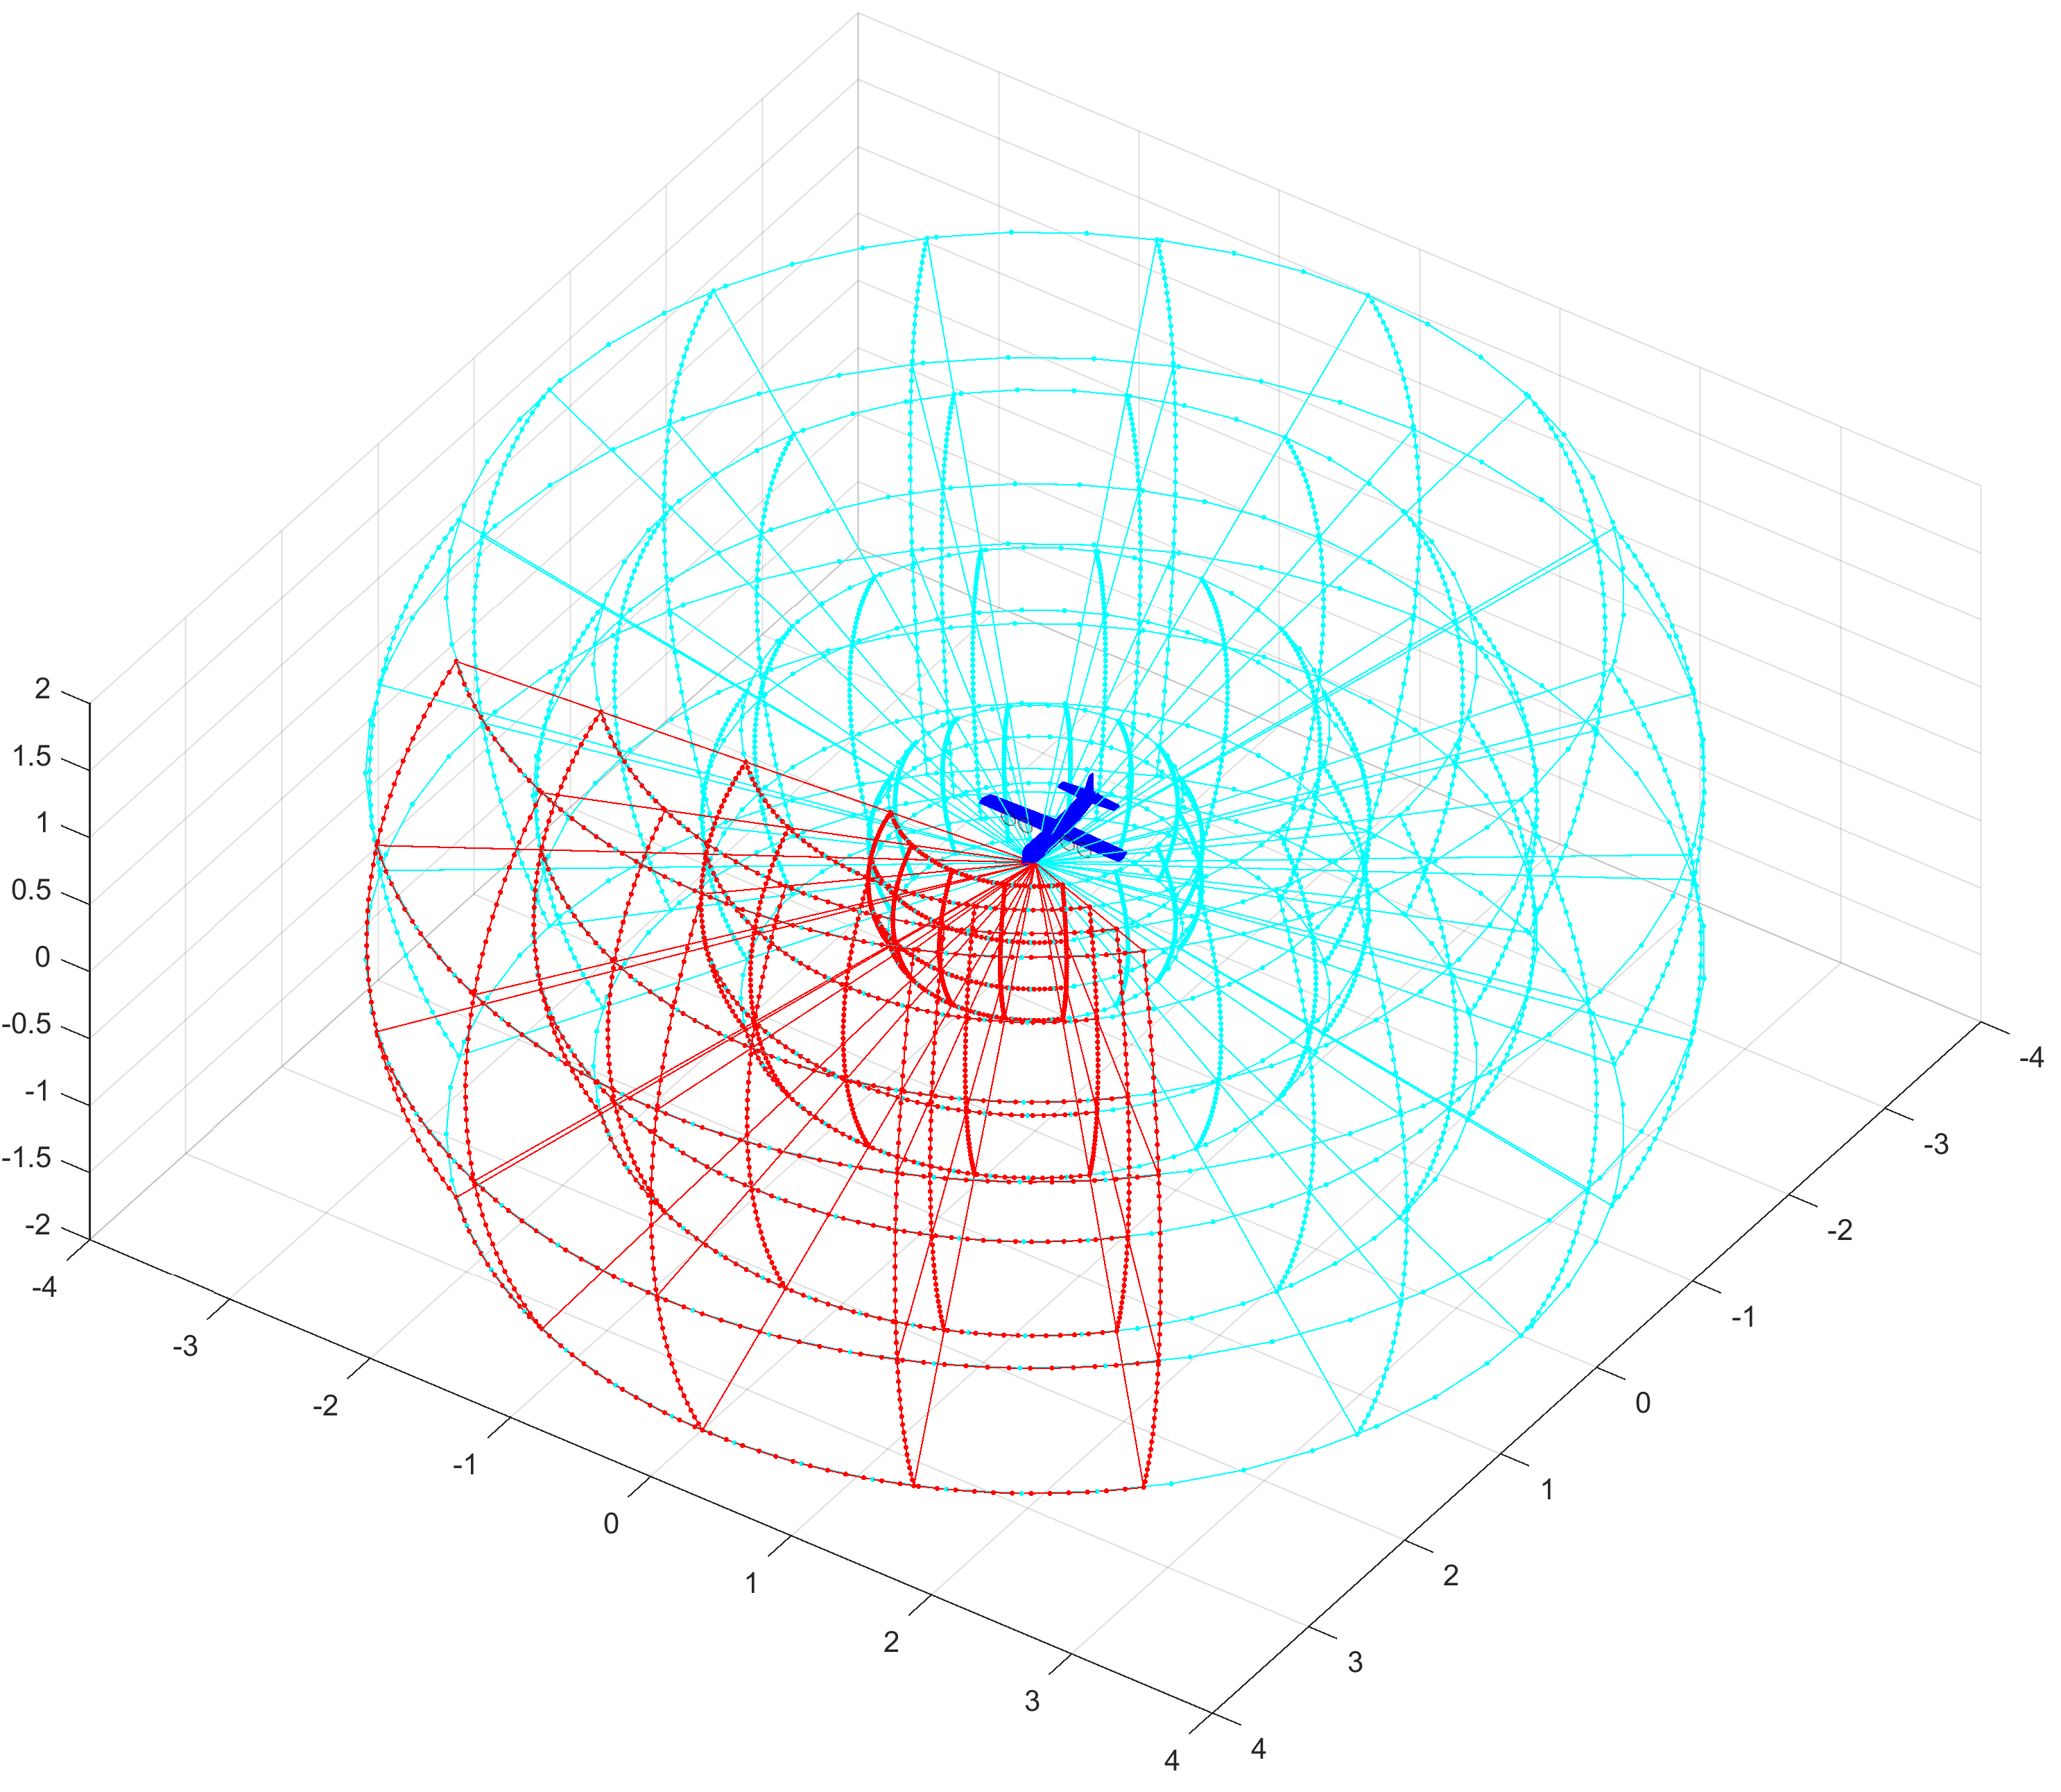
\includegraphics[width=0.80\linewidth]{\FIGDIR/TE046LiDARRasterRange} 
    \caption{Example: The \emph{LiDAR} reading portioning - cells.}
    \label{fig:LidarSpaceSegmentation}
\end{figure}

\paragraph{Avoidance Grid Definition:} The \emph{effective operation space} is going to be portioned into cells. The set of these cells is going to be called \emph{Avoidance Grid}. The idea is to split operational space into cells with even distance, horizontal angle, and vertical angle ranges. 

\begin{definition}{Avoidance Grid}\label{def:AvoidanceGrid} 


\noindent The \emph{effective space portion} (fig. \ref{fig:LidarSpaceSegmentation} red lines) given by a portion of space in UAS local polar coordinate frame, bounded by:
    \begin{enumerate}
        \item \emph{Distance Range} -  in range $distance_{start}$ $<$ $distance_{end}$ $in$ $\R^+$.
        \item \emph{Horizontal Range} - in range by $horizontal^\circ_{start}$ $<$ $horizontal^\circ_{end}$ $\in$ $]-\pi,\pi]$.
        \item \emph{Vertical Range} -in range $vertical^\circ_{start}$ $<$ $vertical^\circ_{end}$ $\in$ $]-\pi,\pi]$.
    \end{enumerate}

\noindent The goal is to separate the \emph{effective operation space} into cells (def. \ref{def:cell}). The idea is to split distance range into multiple distinctive distance ranges with count $layerCount \in \N^+$.  The ranges for \emph{distance layers} are given as follow:
\begin{equation}\label{eq:avoidanceGridCellDistanceRange}
    \begin{aligned}
        layer^i_{start} & = (i-1)\times\frac{distance_{end}-distance_{start}}{layer Count}\\
        layer^i_{end} & = i\times\frac{distance_{end}-distance_{start}}{layer Count}
    \end{aligned};\quad i\in 1\dots layer Count
\end{equation}

\noindent The same separation Layer horizontal/vertical separations separations defined by $horizontal Count \in \N^+$/$vertical Count \in \N^+$:

\begin{equation}\label{eq:avoidanceGridCellHorizontalRange}
    \begin{aligned}
        horizontal^j_{start} & = (j-1)\times\frac{horizontal^\circ_{end}-horizontal^\circ_{start}}{horizontal Count}\\
        horizontal^j_{end} & = j\times\frac{horizontal^\circ_{end}-horizontal^\circ_{start}}{horizontal Count}
    \end{aligned};\quad j\in 1\dots horizontal Count
\end{equation}


\begin{equation}\label{eq:avoidanceGridCellVerticalRange}
    \begin{aligned}
        vertical^k_{start} & = (k-1)\times\frac{vertical^\circ_{end}-vertical^\circ_{start}}{vertical Count}\\
        vertical^k_{end} & = k\times\frac{vertical^\circ_{end}-vertical^\circ_{start}}{vertical Count}
    \end{aligned};\quad k\in 1\dots vertical Count
\end{equation}


\noindent Then $cell_{i,j,k}$ space portion by (def. \ref{def:cell}) has following ranges:
\begin{enumerate}
    \item \emph{Cell Distance Range} (eq. \ref{eq:avoidanceGridCellDistanceRange}) depending on layer index $i$.
    
    \item \emph{Cell Horizontal Angle Range} (eq. \ref{eq:avoidanceGridCellHorizontalRange}) depending on horizontal angle index $j$.
    
    \item \emph{Cell Vertical Angle Range} (eq. \ref{eq:avoidanceGridCellVerticalRange}) depending on vertical index $k$.
\end{enumerate}

\begin{note}
	The example of \emph{Avoidance Grid Cells} is given in (fig. \ref{fig:LidarSpaceSegmentation} red boundary).
\end{note} 

The \emph{Avoidance Grid} is the set of cells:

\begin{equation}\label{eq:avoidanceGridCellSpace}
    Avoidance Grid = \left\{
    					cell_{i,j,k}:
    					\begin{aligned}
    						& i \in 1 \dots layer Count\\
    						& j \in 1 \dots horizontal Count\\
    						& k \in 1 \dots vertical Count
    					\end{aligned} 
                     \right\}
\end{equation}

\begin{note}
	For any distinctive cells $cell_{i,j,k}$, $cell_{m,n,o}$ their \emph{space portion intersection} is empty set:
	\begin{equation}
		\forall cell_{i,j,k}, cell_{m,n,o}:
		\begin{aligned}
		    &cell_{i,j,k}\cap cell_{m,n,o} = \varnothing,
		    i \neq o \lor j \neq n \lor k \neq o
		\end{aligned}
	\end{equation}
\end{note}
\end{definition}

%\paragraph{Trajectory Intersection:} The \emph{trajectory} intersection with \emph{Avoidance Grid} is solved in context of \emph{Reach Set Approximation} (def. \ref{def:ContainedReducedReachSet}). 
%\begin{note}
%    The \emph{trajectory intersection} function does not have an impact on \emph{Reach Set Approximation}, because its done prior the flight.
%\end{note}

\paragraph{Grid Sizing Approach:} The sizing approach used in this work is outlined in (app. \ref{app:gridSizeCalculation}).


\paragraph{Cell in Avoidance Grid Properties:}\noindent For each cell $\vec{p}\in\R^3$ in the there are properties to be checked:

\begin{enumerate}
    \item \emph{Is there visibility to the cell ?} - how good is an observation of the cell by Sensor Field.
    
    \item \emph{Is there threat present ?} - how sure the data fusion is that there is eminent threat in the cell.
    
    \item \emph{Is the cell reachable ?} - if there is any trajectory which can get UAS to that cell without too much threat along the way.
\end{enumerate}

\noindent The answers to these questions are given later in \emph{data fusion procedure}outline (tab. \ref{tab:defuzificationRatings}).
    
	
	%06-06 Reach Set
    \cleardoublepage
\section{\secState{R}Reach Set Approximation}\label{s:reachSet}

    \noindent\paragraph{Motivation:} \emph{Reach set} is strong tool for \emph{Obstacle Avoidance} because it contains all possible \emph{avoidance maneuvers} in set. The current implementation have following flaws:
    
    \begin{enumerate}
        \item \emph{Realistic approximation} - \emph{nonlinear systems} or \emph{heavily constrained systems} cannot be approximated well by \emph{continuous-time Reach Sets}.
        
        \item \emph{Non Deterministic calculations} - continuous-time \emph{Reach Set} contains  infinite possibilities for \emph{avoidance maneuvers}, the SAA system demands conflict resolution in finite time.
        
        \item \emph{Property binding} - binding related properties seems problematic, because \emph{continuous- time reach sets} does not have unique identifier of maneuver, trajectory nor segment. 
    \end{enumerate}
    
    \paragraph{Proposed Solution Features:} Our Reach set Estimation method will provide following features:
    
    \begin{enumerate}
        \item \emph{System Control Interface} - implemented via \emph{Movement Automaton}, requiring only \emph{discrete command chain} to approximate system behaviour.
        
        \item \emph{Deterministic Calculation} - finite number of elements in \emph{Reach set} will enable \emph{scalable} calculation.
        
        \item \emph{Property binding} - approximation of Reach set as a set of trajectories, each trajectory can be split into finite number of segments. Each element will have unique identifier enabling both-side  property binding.
        
        \item \emph{Behaviour encoding} - some specific behaviour, like horizontal/vertical separation, or maneuver shape can be encoded into \emph{Reach Set}.
    \end{enumerate}
    
    
    \paragraph{Discretization of Reach set:} There is a need for a discrete finite \emph{Reach Set approximation} to enable \emph{Avoidance Strategy Evaluation} in finite time. Replacing \emph{Continuous Control Set} \emph{Inputs(t)} by \emph{Movement Automaton} is feasible:
    
    
    \begin{definition}[Reach set Approximation by Movement Automaton]\label{def:ReachSetApproximationByMovementAutomaton}
        \emph{A trajectory} (def. \ref{def:MovementAutomatonTrajectory}) for system $\dot{state}=f(time,state,input)$ under control of the movement automaton $\mathscr{MA}$ is given as execution of movement buffer (def. \ref{def:MovementBuffer}) with initial state of system $state_0$.  Therefore notation $Trajectory(state_0,buffer)$ is used.
    
        
        \paragraph{The Complete Reach Set} (\ref{eq:reachSetFormalDefintion}) for system with initial state $state_0$ with existing \emph{control strategy} $control(time)\in Controls(time)$. for time  $\tau > time_0$.
        \begin{equation}\label{eq:reachSetFormalDefintion}
            ReachSet(\tau,time_0,state_0) = \bigcup \left\{state(s):control(s)\in Controls(s), s\in (time_0,\tau]\right\} 
        \end{equation}
        
        
        \paragraph{The Reach Set Approximation by Movement Automaton} (\ref{eq:ReachSetDefinitionDiscrete}) of the system under the control of the movement automation $\mathscr{MA}$ consist from the set of trajectories $Trajectory$ $(state_0,$ $Buffer)$, which are executed in constrained time $\tau > time_0$.
        \begin{equation}\label{eq:ReachSetDefinitionDiscrete}
             ReachSet(\tau,time_0,state_0)=\left\{Trajectory(state_0,buffer):
             \begin{gathered}
                \text{duration}(buffer)\\ \le\\ (time_0-\tau)
             \end{gathered}\right\}
        \end{equation}
    \end{definition}
    
    \begin{note}
        \emph{Reach Set Approximation} (def. \ref{def:ReachSetApproximationByMovementAutomaton}) is subset of \emph{Full Reach Set} (def. \ref{def:ReachSetBasic}) in continuous space $\R^n$ it inherits all important properties, like \emph{Invariance} \cite{blanchini1999set}.
        
        \emph{Discretization} of \emph{Reach Set} have been achieved leaving us with \emph{finite count} of \emph{Trajectories}, instead of \emph{Infinite subspace or $\R^N$}
    \end{note}

    \paragraph{Approximated Reach Set Containment:} The \emph{Approximated Reach Set} introduced in (def. \ref{def:ReachSetApproximationByMovementAutomaton}) is constrained only by \emph{future expansion time} $\tau$. UAS makes space assessment in \emph{Avoidance Grid}. There is no point to consider Trajectories outside of \emph{Avoidance Grid}
    
    \begin{definition}[Contained Aproximated Reach Set]\label{def:ContainedReducedReachSet}
        For pair ($state_0$, $AvoidanceGrid_0$) at time $time_0$ and \emph{prediction horizon} $\tau=\infty$ there is \emph{Contained Reduced Reach Set:}
        \begin{equation}\label{eq:containedReachSet}
            ReachSet\left(\begin{gathered}time_0,\\state_0,\\AvoidanceGrid_0\end{gathered}\right) = 
            \left\{
                \begin{gathered}
                Trajectory(\dots) \\\in\\ ReachSet(\ref{eq:ReachSetDefinitionDiscrete})
                \end{gathered}
                :
                \begin{gathered}
                \forall segment \in AvoidanceGrid_0,\\ segment \in Trajectory(\dots)    
                \end{gathered}
            \right\}
        \end{equation}
        
        \paragraph{Properties:} \emph{Container Aproximated Reach Set} contains only trajectories where all segments belongs to \emph{Avoidance Grid}, there are following functions:
        \begin{enumerate}
            \item \emph{Membership function} for any \emph{Trajectory} in \emph{Constrained Reduced Reach set} returns \emph{Ordered Set} of \emph{Passing Cells}. 
            
            \item \emph{Cost function} for any \emph{Trajectory Portion} in \emph{Constrained Reduced Reach Set} return \emph{Cost of Execution}
        \end{enumerate}
        
        \paragraph{Passing cell:} \emph{Cell} of \emph{Avoidance Grid} which has some intersection with {Trajectory}.
    \end{definition}
    
    \begin{note}
        \emph{Contained Reduced Reach Set} (eq. \ref{eq:containedReachSet}) which is contained in \emph{Avoidance Grid} and have an \emph{Membership Function} enable Property transition between Reach set and \emph{Avoidance grid}. 
        
        \emph{Example:} Visibility from cells along \emph{Trajectory} can be gathered to calculate \emph{Trajectory`s} feasibility.
    \end{note}
    
    \paragraph{Reach Set Pruning:} There is a need to implement \emph{Set Difference} between \emph{Reach Set} and 
    \emph{Constraint Set}. Constraint Set cam be \emph{Obstacle Set} from \emph{Known World} (sec. \ref{s:KnownWorld}) and other different constraints.
    
    \paragraph{Reach Set Trajectory Tree:} (\ref{eq:trajectoryTree}) \emph{Any Reach Set} where \emph{Control Strategy Constraint} is implemented as \emph{Movement Automaton}, with defined \emph{Movements} set and for singe initial $state_0$. The \emph{Reach Set} is given as discrete tree with root $Trajectory(state_0,\varnothing)$. 
    
    \begin{equation}\label{eq:trajectoryTree}
        ReachSet(state_0,\dots) = \left\{Trajectory(state_0,buffer):
        \begin{gathered}
            buffer\in Movements^i,\\
            i\in\{1,\dots,k\}
        \end{gathered}\right\}
    \end{equation}
    
    \noindent For each \emph{Trajectory Segment}, there exists \emph{intersection function} which evaluates as true if there exists at least one point in \emph{Segment} which belongs to \emph{Constraint Set}. Formally: 
    \begin{equation}\label{eq:reachsetIntersectionConstraintSet}
        intersection(segment,Set):
        \begin{cases}
            \begin{aligned}\exists &point \in segment,\\ &point \in Set \end{aligned}&: true \\
            Otherwise &: false 
        \end{cases}
    \end{equation}
    
    \begin{definition}[Pruned Reach Set]\label{def:PrunedReachSet} 
        For \emph{Reach set} represented as \emph{Trajectory Tree} (eq. \ref{eq:trajectoryTree}) and some constraint set ($Set$) where exist \emph{intersection function} (eq. \ref{eq:reachsetIntersectionConstraintSet}). The \emph{Pruned Reach set} is given as follows:
        
        \begin{equation}\label{eq:PrunedReachSet}
            Prune(ReachSet,Set) = 
            \left\{
                Trajectory(\dots):
                \begin{gathered} 
                \forall segment \in Trajectory,\\ \neg intersection(segment, Set) 
                \end{gathered}
            \right\}
        \end{equation}
    \end{definition}
    
    
    \begin{note} 
        Pruning(def. \ref{def:PrunedReachSet}) \cite{birmingham1988tree} is applicable multiple times for various \emph{Constraints Set}. 
    
        Example of \emph{Approximated Reach set Calculation} (def. \ref{def:ReachSetApproximationByMovementAutomaton}), \emph{Reach Set Containment} (def. \ref{def:ContainedReducedReachSet}), and, \emph{Pruning} is given in \cite{gomola2017obstacle}.
    \end{note}

    	\subsection{Trajectory Set Approximation of Reach Set}\label{sec:trajectory set Reach set approximation}
    \paragraph{Discretization of Reach set:} There is a need for a discrete finite \emph{Reach Set approximation} to enable \emph{Avoidance Strategy Evaluation} in finite time. Replacing \emph{Continuous Control Set} \emph{Inputs(t)} by \emph{Movement Automaton} is feasible:
    
    
    \begin{definition}[Reach set Approximation by Movement Automaton]\label{def:ReachSetApproximationByMovementAutomaton}
        \emph{A trajectory} (def. \ref{def:MovementAutomatonTrajectory}) for system $\dot{state}=f(time,state,input)$ under control of the movement automaton $\mathscr{MA}$ is given as execution of movement buffer (def. \ref{def:MovementBuffer}) with initial state of system $state_0$.  Therefore notation $Trajectory(state_0,buffer)$ is used.
    
        
        \paragraph{The Complete Reach Set} (\ref{eq:reachSetFormalDefintion}) for system with initial state $state_0$ with existing \emph{control strategy} $control(time)\in Controls(time)$. for time  $\tau > time_0$.
        \begin{equation}\label{eq:reachSetFormalDefintion}
            ReachSet(\tau,time_0,state_0) = \bigcup \left\{state(s):control(s)\in Controls(s), s\in (time_0,\tau]\right\} 
        \end{equation}
        
        
        \paragraph{The Reach Set Approximation by Movement Automaton} (\ref{eq:ReachSetDefinitionDiscrete}) of the system under the control of the movement automation $\mathscr{MA}$ consist from the set of trajectories $Trajectory$ $(state_0,$ $Buffer)$, which are executed in constrained time $\tau > time_0$.
        \begin{equation}\label{eq:ReachSetDefinitionDiscrete}
             ReachSet(\tau,time_0,state_0)=\left\{Trajectory(state_0,buffer):
             \begin{gathered}
                \text{duration}(buffer)\\ \le\\ (time_0-\tau)
             \end{gathered}\right\}
        \end{equation}
    \end{definition}
    
    \begin{note}
        \emph{Reach Set Approximation} (def. \ref{def:ReachSetApproximationByMovementAutomaton}) is subset of \emph{Full Reach Set} (def. \ref{def:ReachSetBasic}) in continuous space $\R^n$ it inherits all important properties, like \emph{Invariance} \cite{blanchini1999set}.
        
        \emph{Discretization} of \emph{Reach Set} have been achieved leaving us with \emph{finite count} of \emph{Trajectories}, instead of \emph{Infinite subspace or $\R^N$}
    \end{note}

    \paragraph{Approximated Reach Set Containment:} The \emph{Approximated Reach Set} introduced in (def. \ref{def:ReachSetApproximationByMovementAutomaton}) is constrained only by \emph{future expansion time} $\tau$. UAS makes space assessment in \emph{Avoidance Grid}. There is no point to consider Trajectories outside of \emph{Avoidance Grid}
    
    \begin{definition}[Contained Aproximated Reach Set]\label{def:ContainedReducedReachSet}
        For pair ($state_0$, $AvoidanceGrid_0$) at time $time_0$ and \emph{prediction horizon} $\tau=\infty$ there is \emph{Contained Reduced Reach Set:}
        \begin{equation}\label{eq:containedReachSet}
            ReachSet\left(\begin{gathered}time_0,\\state_0,\\AvoidanceGrid_0\end{gathered}\right) = 
            \left\{
                \begin{gathered}
                Trajectory(\dots) \\\in\\ ReachSet(\ref{eq:ReachSetDefinitionDiscrete})
                \end{gathered}
                :
                \begin{gathered}
                \forall segment \in AvoidanceGrid_0,\\ segment \in Trajectory(\dots)    
                \end{gathered}
            \right\}
        \end{equation}
        
        \paragraph{Properties:} \emph{Container Aproximated Reach Set} contains only trajectories where all segments belongs to \emph{Avoidance Grid}, there are following functions:
        \begin{enumerate}
            \item \emph{Membership function} for any \emph{Trajectory} in \emph{Constrained Reduced Reach set} returns \emph{Ordered Set} of \emph{Passing Cells}. 
            
            \item \emph{Cost function} for any \emph{Trajectory Portion} in \emph{Constrained Reduced Reach Set} return \emph{Cost of Execution}
        \end{enumerate}
        
        \paragraph{Passing cell:} \emph{Cell} of \emph{Avoidance Grid} which has some intersection with {Trajectory}.
    \end{definition}
    
    \begin{note}
        \emph{Contained Reduced Reach Set} (eq. \ref{eq:containedReachSet}) which is contained in \emph{Avoidance Grid} and have an \emph{Membership Function} enable Property transition between Reach set and \emph{Avoidance grid}. 
        
        \emph{Example:} Visibility from cells along \emph{Trajectory} can be gathered to calculate \emph{Trajectory`s} feasibility.
    \end{note}
    
    \paragraph{Reach Set Pruning:} There is a need to implement \emph{Set Difference} between \emph{Reach Set} and 
    \emph{Constraint Set}. Constraint Set cam be \emph{Obstacle Set} from \emph{Known World} (sec. \ref{s:KnownWorld}) and other different constraints.
    
    \paragraph{Reach Set Trajectory Tree:} (\ref{eq:trajectoryTree}) \emph{Any Reach Set} where \emph{Control Strategy Constraint} is implemented as \emph{Movement Automaton}, with defined \emph{Movements} set and for singe initial $state_0$. The \emph{Reach Set} is given as discrete tree with root $Trajectory(state_0,\varnothing)$. 
    
    \begin{equation}\label{eq:trajectoryTree}
        ReachSet(state_0,\dots) = \left\{Trajectory(state_0,buffer):
        \begin{gathered}
            buffer\in Movements^i,\\
            i\in\{1,\dots,k\}
        \end{gathered}\right\}
    \end{equation}
    
    \noindent For each \emph{Trajectory Segment}, there exists \emph{intersection function} which evaluates as true if there exists at least one point in \emph{Segment} which belongs to \emph{Constraint Set}. Formally: 
    \begin{equation}\label{eq:reachsetIntersectionConstraintSet}
        intersection(segment,Set):
        \begin{cases}
            \begin{aligned}\exists &point \in segment,\\ &point \in Set \end{aligned}&: true \\
            Otherwise &: false 
        \end{cases}
    \end{equation}
    
    \begin{definition}[Pruned Reach Set]\label{def:PrunedReachSet} 
        For \emph{Reach set} represented as \emph{Trajectory Tree} (eq. \ref{eq:trajectoryTree}) and some constraint set ($Set$) where exist \emph{intersection function} (eq. \ref{eq:reachsetIntersectionConstraintSet}). The \emph{Pruned Reach set} is given as follows:
        
        \begin{equation}\label{eq:PrunedReachSet}
            Prune(ReachSet,Set) = 
            \left\{
                Trajectory(\dots):
                \begin{gathered} 
                \forall segment \in Trajectory,\\ \neg intersection(segment, Set) 
                \end{gathered}
            \right\}
        \end{equation}
    \end{definition}
    
    
    \begin{note} 
        Pruning(def. \ref{def:PrunedReachSet}) \cite{birmingham1988tree} is applicable multiple times for various \emph{Constraints Set}. 
    
        Example of \emph{Approximated Reach set Calculation} (def. \ref{def:ReachSetApproximationByMovementAutomaton}), \emph{Reach Set Containment} (def. \ref{def:ContainedReducedReachSet}), and, \emph{Pruning} is given in \cite{gomola2017obstacle}.
    \end{note}

    	\subsection{\secState{R}Reach Set Performance Criteria}\label{s:ReachSetPerformanceCriteria}

\paragraph{Motivation:} The need to Make \emph{Reach Set} scalable approach. This may be a problem due the \emph{Expansion rate}. \emph{Reach set} represented as a \emph{Trajectory Tree} (eq. \ref{eq:trajectoryTree}) for Avoidance Grid with $layerCount$ and Movement automaton with $movementCount$, the \emph{Node count} is given as:

\begin{equation}\label{eq:fullReachSetNodeCount}
    1+ \left(\sum_{i\in\{1\dots layerCount\}} (movementCount)^i\right)
\end{equation}

\noindent \emph{This scaling} is not feasible for \emph{Avoidance Grid} with many layers ($< 10$) or \emph{Movement Set} with many movements ($< 9$). There is need for \emph{Reduced Reach set calculation}.

\paragraph{Core Performance Criteria:} The scaling factor (eq. \ref{eq:fullReachSetNodeCount}) shows that there are going to be many trajectories. The main point is that not every trajectory in \emph{Reach Set} are giving us \emph{maneuverability advantage}. Our expectations lies in following \emph{Performance Requirements}:

\begin{enumerate}
    \item \emph{Reach set} must \emph{Cover} maximum of the \emph{possible unique maneuvers} in  \emph{Avoidance Grid}.
    \item \emph{Trajectories} in \emph{Reach Set} should be smoothest possible to prevent cargo damage / UAS wear.
\end{enumerate}

\paragraph{Trajectory footprint:} Discrete space of \emph{Avoidance Grid} is organized in cells. \emph{Cell} is minimal space portion accessible by \emph{property binding}. There is need to know if two trajectories contribution to \emph{Maneuverability} in this environment. 

Each trajectory passes through space in \emph{Avoidance Grid}. If there exists a method to extract unique identifier for each \emph{trajectory passed cells}, we can compare two trajectories \emph{Coverage} in \emph{Avoidance Grid}.


\begin{definition}[Trajectory footprint] \label{def:trajectoryFootprint}
    For \emph{Trajectory} from \emph{Reach set} (def. \ref{def:ContainedReducedReachSet}) defined for \emph{Avoidance Grid} has membership function. \emph{Membership Function} returns \emph{ordered set of passing cells}:
    
    \begin{equation}\label{eq:setOfPassedCells}
        footprint
        \left(\begin{gathered}
            Trajectory,\\
            AvoidanceGrid    
        \end{gathered}\right) 
        = 
        \left\{
            \begin{aligned}
                cell \in& AvoidanceGrid:\\ &isMember(trajectory,cell)
            \end{aligned}
        \right\}
    \end{equation}
    
    \noindent Then we can define equality function for $Trajectory_1$ and $Trajectory_2$, as comparison of their footprints in common \emph{Avoidance Grid} as follow:
    
    \begin{equation}\label{eq:TrajectoryEquality}
        isEqual\left(\begin{gathered}
        Trajectory_1,\\Trajectory_2,\\AvoidanceGrid  
        \end{gathered}\right):
        \begin{cases}
            \left(\begin{gathered}
                footprint(Trajectory_1,\dots)\\
                = \\
                footprint(Trajectory_2,\dots)
            \end{gathered}\right)
            &:true\\
            Otherwise&: false\\
        \end{cases}
    \end{equation}
\end{definition}

\begin{note}
    Depending on \emph{Movement Automaton`s} movement set and \emph{Avoidance Grid} parameters, there can be multiple \emph{trajectories} which are equal.
\end{note}

\paragraph{Coverage set:} Now it is possible to create set of unique \emph{trajectory footprints} due to \emph{footprint function} (eq. \ref{eq:setOfPassedCells}). Similarly there is a possibility to create \emph{Reach set skeleton} containing unique trajectories, by using 
\emph{equality function} (eq. \ref{eq:TrajectoryEquality}).
\emph{Coverage set} is sufficient for now.

\newpage
\begin{definition}[Coverage Set]\label{def:CoverageSet}
    \emph{Coverage set} (\ref{eq:CoverageSet}) is defined for \emph{Avoidance Grid} and \emph{Reach Set} pair as set of unique \emph{Trajectory footprints}:
    
    \begin{equation}\label{eq:CoverageSet}
        CoverageSet\left(\begin{gathered}AvoidanceGrid,\\ReachSet\end{gathered}\right)= \left\{
            footprint\left(\begin{gathered}     
                Trajectory,\\AvoidanceGrid
            \end{gathered}\right):
            \begin{aligned}
                \forall &Trajectory\\ &\in Reach Set
            \end{aligned}\right\}
    \end{equation}
\end{definition}

\paragraph{Coverage set properties:} Trajectory footprint (eq. \ref{eq:setOfPassedCells})is not \emph{bijection}, neither \emph{injection} for $ReachSet \to CoverageSet$. This implies following properties:

\begin{enumerate}
    \item Equal \emph{Reach Sets} in same \emph{Avoidance Grid} have equal \emph{Coverage Sets}.
    
    \item Equal \emph{Coverage Sets} does not imply \emph{Reach Set} equality.
    
    \item For two {Coverage Sets} there is a possibility to compare their member count to create coverage ratio.
\end{enumerate}

The second \emph{Property} gives us a preposition that there is a possibility of \emph{Reach Set Reduction} without loosing 
\emph{Coverage}.  

\begin{definition}[Coverage Ratio]\label{def:coverageRatio}
    \emph{Coverage Ratio} is a ratio of \emph{Coverage Set Member Count} between two \emph{Reach Sets}. Reach set with \emph{lesser count of unique Trajectories} is considered as \emph{Reduced Reach Set}.  Reach set with \emph{greater Count of unique Trajectories} is considered as \emph{Reference Reach Set}.
    
    \begin{equation}\label{eq:CoverageRatio} 
        \begin{gathered}
            referenceCoverage=|CoverageSet(ReferenceReachSet,AvoidanceGrid)|\\
            reducedCoverage=|CoverageSet(ReducedReachSet,AvoidanceGrid)|\\
            CoverageRatio = \frac{reducedCoverage}{referenceCoverage}\in[0,1]
        \end{gathered}
    \end{equation}
\end{definition}

\begin{note}
    \emph{Reference Reach Set} is usually \emph{Full Reach Set} containing all possible trajectories in space contained by \emph{Avoidance Grid}. In case \emph{Full Reach Set} cannot be computed, Avoidance Grid is too large, most complex \emph{Reach Set} is used as \emph{Reference Reach Set}.
\end{note}

\paragraph{Trajectory smoothness:} Trajectory other than straight line have some changes in \emph{UAS} heading. 

The goal is to minimize \emph{Maneuvering} of UAS, because:
\begin{enumerate}
    \item \emph{Every Heading Change} needs to be reported to \emph{UTM}.
    \item \emph{Sharp Maneuvering} can damage cargo/wear UAS.
    \item \emph{Often course changes} makes \emph{Intruder prediction} harder for other Civil General Aviation.
\end{enumerate}

\noindent For this purpose \emph{Smoothness Metric} needs to be applied for \emph{Reach Set} or \emph{Trajectory}.  In case of \emph{Movement Automaton Control} two distinguish \emph{Movement Sets} can be introduced:\emph{Smooth} nad \emph{Chaotic} movements set with following properties:

\begin{equation}\label{eq:ChaoticSmoothMovementSetDefinition}
    \begin{gathered}
        MovementSet=SmoothMovements\cup ChaoticMovements\\
        SmoothMovements\cap ChaoticMovements = \varnothing\\
        |SmoothMovements| > 0, \quad |ChaoticMovements|>0
    \end{gathered}
\end{equation}

Then \emph{Smoothnes clasificator} for $Trajectory(initialState,buffer)$ can be defined as $isSmooth$ and \emph{Smooth Movement Counter} function as $smoothCount$ like follow:

\begin{equation}\label{eq:SmoothnesClasificatorCounter}
    \begin{gathered}
        isSmooth(movement)=
        \begin{cases}
            movement \in SmoothMovements &:1\\
            movement \in ChaoticMovements &:0
        \end{cases}\\
        smoothCount(Trajectory(\dots,buffer))= 
        \begin{aligned}
            \sum isS&mooth(movement),\\& \forall movement \in Buffer
        \end{aligned}
    \end{gathered}
\end{equation}

\begin{definition}[Smoothness Rating for Trajectory]\label{def:SmoothnessRatingForTrajectory} 
    \emph{Smoothness} for trajectory generated by \emph{Movement Automaton} for some \emph{Initial State} with some \emph{Movement Buffer}, under assumption of \emph{Smooth and Chaotic Movement Set} split (eq. \ref{eq:ChaoticSmoothMovementSetDefinition}), with existing \emph{classification} and \emph{counter} functionals (eq. \ref{eq:SmoothnesClasificatorCounter}) is given as follows:

    \begin{equation}
        Smoothness(Trajectory(\dots,buffer)) = \frac{isSmooth(Trajectory)}{movementCount(Trajectory)} \in [0,1] 
    \end{equation}
    
    \noindent For \emph{Trajectory} with $buffer=\varnothing$ \emph{Smoothness} is given as 1.
\end{definition}

    	\subsection{\secState{R}Constrained Trajectory Expansion}\label{s:constrainedTrajectoryExpansion}

\paragraph{Motivation:} \emph{Purpose} of \emph{Navigation} is to move forward to \emph{Goal Waypoint} in \emph{Mission}. \emph{Structure} of \emph{Avoidance Grid} is designed to enable \emph{forward} and \emph{turning} maneuvers. The \emph{Avoidance Grid} is organized in \emph{Layers} characteristic by same distance from \emph{Avoidance Grid Origin}. 

Survey of motion planning algorithm was given in \cite{goerzen2009survey}. The ideal candidate for propagation algorithm is \emph{Wave-front} algorithm propagating \emph{Trajectory tree} through Layers. Due the \emph{Avoidance Grid} onion like layers, there is possibility to implement turn maneuver through layers iterative and effectively .

\begin{figure}[H]
    \centering
    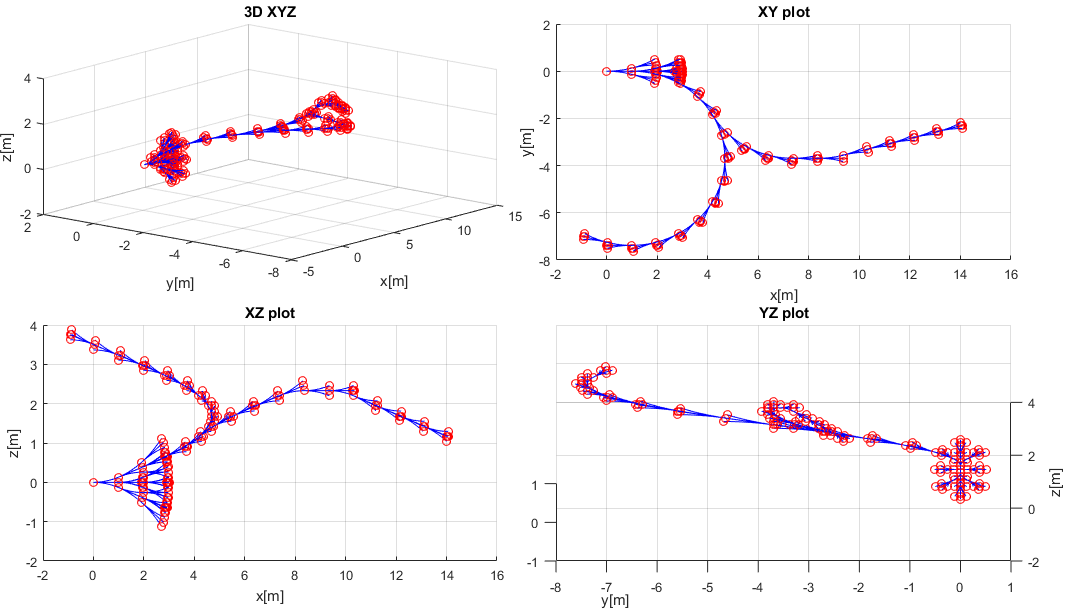
\includegraphics[width=0.9\linewidth]{\FIGDIR/RS001RapidExplorationTreeExampleShrink} 
    \caption{\emph{Rapid Exploration tree as result of \emph{Constrained trajectory expansion}}.}
    \label{fig:rapidExplorationTrajectoryTree}
\end{figure}

\paragraph{Rapid Exploration Tree} (fig. \ref{fig:rapidExplorationTrajectoryTree}) was selected, because it enables \emph{Movement Automaton Utilization} and \emph{Property Binding}. Similar approach was used for space exploration \cite{plaisant2002spacetree}. 

\paragraph{The example} (fig. \ref{fig:rapidExplorationTrajectoryTree}) shows a \emph{Rapid Exploration Tree} in \emph{Free Space} containing \emph{Waypoint Navigation Path} and \emph{Turn Away Path}. Both paths are starting in same \emph{Root Node} (red circle) which was expanded with simple \emph{Movement Automaton} (bunch of nodes originating from one node are showing way of expansion). The connection (blue line) between two nodes (red circles) represents \emph{Trajectory portion} for \emph{Executed Movement}.

\paragraph{Rapid Exploration Tree Node} will contain following information:
\begin{enumerate}
    \item \emph{Initial state} - root entry point, used in state evolution calculation.
    \item \emph{Trajectory (state evolution)} - trajectory passing through \emph{state space} in local coordinate frame of \emph{Avoidance Grid}.
    \item \emph{Buffer} (applied movements) - ordered list of \emph{executed movements} applied on \emph{initial state} to obtain \emph{state evolution}.
    \item \emph{Cost} - calculated for \emph{state evolution} based on \emph{predefined cost function}. 
    \item \emph{Footprint} - ordered set of \emph{passing cells} in \emph{Avoidance Grid}.
    \item \emph{Parent Node Reference} - tree reference for parent node, not in case of \emph{root node}.
    \item \emph{Other Bounded Properties} - value list of other properties, depending on \emph{Expansion Constraints} and \emph{Reachability} evaluation algorithm.
\end{enumerate}

\paragraph{Wave-front propagation of Rapid Exploration Tree} is given in (alg. \ref{alg:Wavefront Propagation}). 

The \emph{Avoidance Grid} have UAS with \emph{position $\in$ Initial State} at the \emph{origin}. The \emph{Grid Layer} is a column ordered set of cells with same \emph{Mean distance} from origin. \emph{Grid Layers} are indexed from origin starting with $1$, there is maximum of \emph{i $\ge$ 1} layers.

\paragraph{Step: Initialization} contains base structure preparation like follows:
\begin{enumerate}
    \item \emph{Avoidance Grid} - Space containing \emph{Reach set} (def. \ref{def:ContainedReducedReachSet}).
    \item \emph{Movement Automaton} - Used as \emph{Predictor}, consuming \emph{buffer} containing \emph{Movements} to generate $Trajectory(initialState,buffer)$.
    
    \item \emph{Reach Set} -  tree consisting from \emph{Wave-frontNodes} representing the end point of $Trajectory(initialState,buffer)$ where each \emph{Edge} represents \emph{one Movement application}. The root is set as node containing \emph{Initial State}.
\end{enumerate}

\noindent Function \emph{initializeReachSet(root,stack,grid,automaton)} will take the root and enforces \emph{full wavefornt propagation} to \emph{First Layer}.


\paragraph{Step: Wave-front Propagation} is forced propagation of trajectories from layer $i$ to layer $i+1$. The process goes as follows:
\begin{enumerate}
    \item \emph{Selection of Feasible candidates} - function \emph{[candidates,leftovers] = ExpansionConstraints.select(stack)} for working layer, row and cell selects \emph{feasible trajectory nodes} ordered by \emph{Cost function}. The \emph{Example of Cost Function} can be \emph{Trajectory Smoothness} (def. \ref{def:SmoothnessRatingForTrajectory}).
    
    \item \emph{Expansion of Candidates} - for each \emph{candidate} function \emph{candidate.expandNode (automaton)} is invoked. This function will expand \emph{Candidate Node structure} by appending \emph{Full Trajectory Tree Evolution} until each \emph{Leaf Trajectory} reaches \emph{Next Layer}. Simply put \emph{Par rent Node} \emph{Node(initialState, buffer, cost, footprint )} buffer is appended by movements until the next layer is reached.
    
    \item \emph{Leftovers purge} - function \emph{reachSet.purge(leftovers)} removes unexpanded \emph{Nodes} leading to cell, effectively  removing trajectories which does not  lead to \emph{next layer}.
    
    \item \emph{Append Reach Set} - function \emph{reachSet.append(leafs)} puts newly created \emph{Nodes (Trees)} into \emph{Reach Set} structure. The \emph{Wave-front Propagation} for one cell is finished.
\end{enumerate}

\paragraph{Step: After Layer Propagation Purge} is covered by function \emph{reachSet.purgeSame- Footprint()} which takes trajectories with same footprint and keeps some of them based on \emph{Selection criteria}, more in (sec. \ref{s:chaoticReachSet}, \ref{s:harmonicReachSet}). \emph{Pruning methods} over \emph{Large Decision Trees} are \emph{fast} and \emph{viable} \cite{mingers1989empirical}.

\begin{note}
    \emph{Reach Set} is usually computed \emph{Prior the Flight} for \emph{some Initial State} in \emph{Local Coordinate Frame} in \emph{right had coordinate frame} with $X^+$ used as \emph{main axis}.
\end{note}


\begin{algorithm}[H]
    \SetKwInOut{Input}{Input}\SetKwInOut{Output}{Output}
    \Input{Node(initialState,buffer=$\varnothing$,cost=0,footprint=$\varnothing$),
           AvoidanceGrid, ExpansionConstraints, MovementAutomaton(movementSet)
    }
    \Output{ReachSet(AvoidanceGrid)}
    \BlankLine
    \# Initialization Sequence\;
    grid=AvoidanceGrid, automaton=MovementAutomaton, root = Node\;
    reachSet = initializeReachSet(root,stack,grid,automaton)\;
    \BlankLine
    \# Main Expansion through, layers (i), rows (j), cells(k)\;
    \For{layer($1\dots i$) \emph{in} grid}{
        \For{row($1\dots j$ \emph{in} layer)}{
            \For{cell($1 \dots k$) \emph{in} row}{
                \BlankLine
                \# apply selection criteria \;
                [candidates,leftovers] = ExpansionConstraints.select(stack)\;
                \BlankLine
                \# collect expansions \;
                leafs = []\;
                \For{candidate \emph{in} Candidates}{
                    leafs= [leafs, candidate.expandNode(automaton)];
                }
                reachSet.purge(leftovers)\;
                reachSet.append(leafs)\;
            }
        }
        reachSet.purgeSameFootprint()\;
    }
    \caption{\emph{Wave-front propagation} of \emph{Rapid Exploration Tree} to form \emph{Reach Set}.}
    \label{alg:Wavefront Propagation}
\end{algorithm}






    	\subsection{Coverage-Maximizing Reach Set Approximation}\label{s:chaoticReachSet}

\paragraph{Summary:}

\paragraph{Motivation:} Design of calculation method for \emph{Reach Set Approximation} guarantying high \emph{Maneuverability}.

\paragraph{Background:}There is \emph{Coverage Ratio} property of \emph{Reach Set} (def. \ref{def:coverageRatio}). It has been shown that creating \emph{Reach Set} via \emph{greedy approach} is not feasible due to the \emph{Scaling Factor}.  \emph{Contracted Expansion} (sec. \ref{s:constrainedTrajectoryExpansion}) is enabling to apply selection criteria while building \emph{Reach Set} in given \emph{Cell}. 

The \emph{Cell} $cell_{i,j,k}$ has a center and walls from UAS viewpoint: a front wall, back wall (for $layer > 1$), a top wall, left wall, right wall, bottom wall. It is expected that trajectory leading close to one cell walls will continue to a different cell, increasing the chance to obtain more \emph{Unique Footprints}. 

\paragraph{Expansion Constraint Function Implementation} (alg. \ref{alg:ExpansionConstraintFunctionForChaoticReachSet}) is based on the simple principle: \emph{Select candidate Nodes which are  closest to outer walls of Cell, with a unique footprint}.

\paragraph{Tuning Parameters:} \emph{Proximity to Cell outer wall} gives good chances to break into other rows or columns in the \emph{Avoidance Grid}. \emph{Unique footprint} guarantees future \emph{Unique Footprint} after appending Trajectory by \emph{Movement application}. 
\begin{enumerate}
    \item \emph{Considered Footprint Length} - how much last cells in footprint should be considered in unique path track, minimal value 1, default value 3, maximal value $\infty$. If there is a need to generate non-redundant trajectories use $\infty$, it will consider full footprint.
    
    \item \emph{Spread Limit} - the upper limit of candidates which are going to be select for further expansion, minimal value 1, default value \emph{Count of unique Moves in Movement set}, maximal value $\infty$. If more than default values are selected, the algorithm will generate \emph{redundant trajectories}. If less is selected, then some trajectories are omitted, and \emph{Coverage Rate} decreases sharply. 
\end{enumerate}

\paragraph{Step: Initialization} initialization of \emph{candidate} array (return value), \emph{leftovers} array (return Value). Node array \emph{passing} is populated with \emph{Nodes} which represents \emph{end node of Trajectory}, and the tip of the  \emph{trajectory is constrained in the \emph{cell}$_{i,j,k}$}.

\paragraph{Step: Evaluate best trajectories with unique Footprints} following steps are executed:
\begin{enumerate}
    \item \emph{Best Performance Map} is created with a \emph{footprint} as a key set element to ensure footprint uniqueness.
    
    \item \emph{Wall distance} for the \emph{test node} is calculated as a closest trajectory portion distance to the \emph{top, bottom, left, right} wall of the $cell_{i,j,k}$
    
    \item The \emph{Footprint} for the \emph{test node} is created with the  maximal length given by \emph{Footprint Length} tuning parameter.
    
    \item \emph{Existence and Performance Test} is executed to ensure that the best performing node is selected. If there is no key entry in the \emph{Best Performance Map}, then a new entry for \emph{Test Node} is created. If there is a key entry, the performance of \emph{Old Node} and \emph{Test Node} is compared, and better is stored.
\end{enumerate}

\paragraph{Step: Select candidates} is executed on \emph{Best Performance Map} records using  \emph{Wall distance} as pivot parameter, ordering by closest proximity and limited by \emph{Search Limit} tuning parameter. The \emph{Leftovers} are difference set between \emph{Passing Nodes} and \emph{Candidate Nodes}. 


\begin{algorithm}[H]
    \SetKwInOut{Input}{Input}\SetKwInOut{Output}{Output}\SetKwInOut{TuningParameters}{Tuning Parameters}
    \Input{Node[] stack, Cell cell$_{i,j,k}$}
    \TuningParameters{int$^+$ footprintLength, int$^+$ spreadLimit}
    \Output{Node[] candidates, Node[] leftovers}
    
    \BlankLine
    \# Initialize structures\;
    Node[] candidates = [], Node[] leftovers=[]\;
    Node[] passing = cell$_{i,j,k}$.getFinishingTrajectories(stack)\;
    
    \BlankLine
    \# Select best performing trajectories with unique footprint\;
    Map$<$Footprint,Node$>$  bestPerformanceMap\;
    \For{Node test $\in$ passing}{
        wallDistance= test.minimalDistanceToWall(cell$_{i,j,k}$)]\;
        footPrint = test.getFootprint(lastCells = footprintLength)\;
        \eIf{bestPerformanceMap.contains(footPrint)}{
            old = bestPerformanceMap.getByKey(footprint)\;
            oldPerformance= old.minimalDistanceToWall(cell$_{i,j,k}$)\;
            \If{oldPerformance $>$ wallDistance}{
                bestPerformanceMap.setByKey(footprint,test)\;         
            }
        }{
            bestPerformanceMap.setByKey(footprint,test)\;
        }
    }
    
    \BlankLine
    \# Select best performing nodes up to \emph{spreadLimit} count\;
    candidates = bestPerformanceMap.select(count = spreadLimit).orderBy('wallDistance','Ascending')\;
    leftovers = passing - candidates\;
    \Return{[candidates,leftovers]}
    
    
    \caption{Expansion Constraint function for \emph{Coverage-Maximizing Reach Set Approximation}}
    \label{alg:ExpansionConstraintFunctionForChaoticReachSet}
\end{algorithm}


\paragraph{Example:} for \emph{Avoidance Grid} with \emph{Distance 10 m}, \emph{Layer count 10}, \emph{Horizontal range $[-45^\circ,+45^\circ]$}, \emph{Horizontal Cell Count 7}, \emph{Vertical range $[-30^\circ,+30^\circ]$}, and \emph{Vertical Cell Count 5}. Is given in (fig. \ref{fig:chaoticReachSetApproximation}). The UAS is at \emph{Back-side} of \emph{Figure} (initial state is at all \emph{Trajectory Origins}). The \emph{black dashed line} marks \emph{Avoidance Grid} space boundary. Each trajectory has its own color and ends at \emph{Front-side} of \emph{Avoidance Grid Boundary}.

\begin{figure}[H]
    \centering
    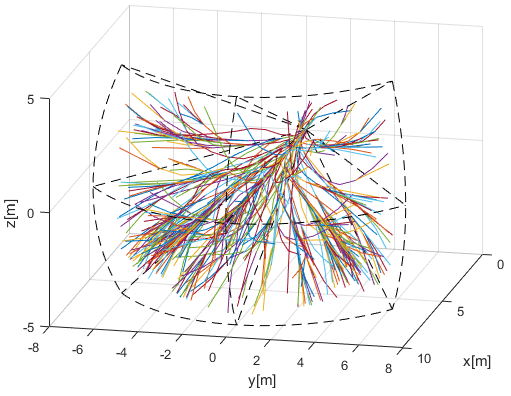
\includegraphics[width=0.7\linewidth]{\FIGDIR/RS002ChaoticReachSetEstimationMethod} 
    \caption{\emph{Coverage-Maximizing \emph{reach set} approximation}.}
    \label{fig:chaoticReachSetApproximation}
\end{figure}


\paragraph{Pros and Cons:} It can be seen from example (fig. \ref{fig:chaoticReachSetApproximation}) that \emph{Coverage-Maximizing Reach Set Approximation Method} (alg. \ref{alg:ExpansionConstraintFunctionForChaoticReachSet}) generates much \emph{turning} and \emph{shaky} \emph{trajectories}. 

\emph{High Coverage Ratio} ($\sim 0.9$) is provided while keeping \emph{medium node count}. The calculation complexity scales linearly with grid size. The \emph{upper limit of trajectories} is given as follow:

\begin{multline}
    countTrajectories(ReachSet) \le layerCellCount \times spreadLimit\\ \times size(Movements)
\end{multline}

\noindent The \emph{upper limit of nodes} is given as follow:
    
\begin{multline}
    countNodes(ReachSet) \le layerCount \times  layerCellCount  \\
    \times size(Movements) \times spreadLimit  
\end{multline}

\noindent The \emph{absence} of \emph{Smooth Trajectories} disqualifies \emph{Coverage Maximizing -RSA} to be used for \emph{Navigation}. This type of reach set is feasible for \emph{Avoidance} because it contains a variety of maneuvers.



    	\subsection{Turn-Minimizing Reach Set Approximation}\label{s:harmonicReachSet}

\paragraph{Motivation:} Imagine having an \emph{Avoidance Grid} like (fig. \ref{fig:LidarSpaceSegmentation}). There is a need of \emph{Reach Set Approximation} which will have \emph{Smooth Trajectories} (def. \ref{def:SmoothnessRatingForTrajectory}) going nearby $cell$ centers.

\paragraph{Background:} The \emph{Smoothness Rating for Trajectory} (def. \ref{def:SmoothnessRatingForTrajectory}) uses two distinct sets \emph{Smooth Movements} and \emph{Chaotic Movements} (eq. \ref{eq:ChaoticSmoothMovementSetDefinition}) which are defined for our \emph{Movement Automaton}  (sec. \ref{s:modelMAImplementation}) like follow:

\begin{equation}
    \begin{aligned}
    Smooth Movements &= \{Straight\} \\
    Chaotic Movements &= Movements - Smooth Movements\\
    \end{aligned}
\end{equation}

\emph{Smooth Movements} contains only \emph{Straight} movement, because others are considered as extreme turning movements. \emph{Smooth Movements} should contain only direct flight movements or slight heading correction. \emph{Chaotic Movements} set is supplement of \emph{Movement Automaton`s Movement Set}. 

The \emph{Avoidance Grid} (fig. \ref{fig:LidarSpaceSegmentation}) cell centers for fixed indexes $j_{fix}$, $k_{fix}$ are linearly aligned with \emph{initial state}. That means that  cell centers of cells $cell_{1,j_{fix},k_{fix}},\dots, cell_{i,j_{fix},k_{fix}}$, where $i$ is count of \emph{layers} lies on one line.  If the trajectory can achieve \emph{cell center} on some \emph{layer} only minor trajectory corrections are required to stay on given line. This type of trajectory gives us following advantages:
\begin{enumerate}
    \item\emph{Minimal steering at beginning} - the minimal steering is advantageous in \emph{Controlled Airspace} because is diminishing the amount of communication to \emph{UTM Service}.
    
    \item\emph{Additional safe space in Linear segment} - once the \emph{center of cell} is reached, \emph{Trajectory} sticks to line between cell centers. Each point on this line has \emph{maximal distance} to outer walls of cell. This gives us extra space given as minimum of distance between \emph{UAS position} and \emph{Outer cell walls}.
\end{enumerate}

\paragraph{Expansion Constraint Function Implementation} (alg. \ref{alg:ExpansionConstraintFunctionForHarmonicReachSet}) is based on simple principle: \emph{Select candidate Nodes  which are closest to Cell center, with unique footprint}.

\begin{note}
    \emph{Cell center} can be closely reached by \emph{smooth movement} from previous cell or \emph{chaotic movement} from neighbouring cell from current or previous layer. These trajectories are usually equivalent in \emph{Smoothness}.
\end{note}

\paragraph{Tuning Parameter:} \emph{Proximity to Cell Center} gives a good chance to keep trajectory smooth or \emph{smooth after one correction maneuver}. It has been mentioned that \emph{Cell Center} can be reached by various trajectories. In this method full footprint length is always considered, therefore only one tuning parameter can be offered:
\begin{enumerate}
    \item \emph{Spread Limit} - upper limit of candidates which are going to be selected for further expansion, minimal value 1, default value \emph{Count of unique Moves in Movement set}, maximal value $\infty$. If maximal value $\infty$ is selected, algorithm will generate skeleton of \emph{Reach Set} with full Coverage and with the smoothest \emph{Trajectories}.
\end{enumerate}

\paragraph{Step: Initialization} sets candidate \emph{Nodes} as empty set, leftover \emph{Nodes} as empty set. and selects all \emph{Nodes} from \emph{Stack} which represents  \emph{Finishing Trajectories} in working cell $cell_{i,j,k}$.

\begin{algorithm}[H]
\SetKwInOut{Input}{Input}\SetKwInOut{Output}{Output}\SetKwInOut{TuningParameters}{Tuning Parameters}
    \Input{Node[] stack, Cell cell$_{i,j,k}$}
    \TuningParameters{int$^+$ spreadLimit}
    \Output{Node[] candidates, Node[] leftovers}
    
    \BlankLine
    \# Initialize structures\;
    Node[] candidates = [], Node[] leftovers=[]\;
    Node[] passing = cell$_{i,j,k}$.getFinishingTrajectories(stack)\;
    
    \BlankLine
    \# Select unique smoothest trajectories\;
    Map$<$Buffer,Node$>$  bestPerformanceMap\;
    \For{Node test $\in$ passing}{
        centerDistance= test.getPerformance(cell$_{i,j,k}$)]\;
        footPrint = test.getFootprint()\;
        \eIf{bestPerformanceMap.contains(footPrint)}{
            old = bestPerformanceMap.getByKey(footprint)\;
            oldPerformance= old.getPerformance(cell$_{i,j,k}$)\;
            \If{oldPerformance $>$ centerDistance}{
                bestPerformanceMap.setByKey(footprint,test)\;         
            }
        }{
            bestPerformanceMap.setByKey(footprint,test)\;
        }
    }
    
    \BlankLine
    \# Select best performing nodes up to \emph{spreadLimit} count\;
    candidates = bestPerformanceMap.select(count = spreadLimit).orderBy('cellCenterDistance','Ascending')\;
    leftovers = passing - candidates\;
    \Return{[candidates,leftovers]}
    
    
    \caption{Expansion Constraint function for \emph{Harmonic Reach Set Approximation}}
    \label{alg:ExpansionConstraintFunctionForHarmonicReachSet}    
\end{algorithm}

\paragraph{Step: Evaluate smoothest trajectories with unique Footprints} is implemented as \emph{multi-criteria filtration}. 

\emph{First criterion} is \emph{distance to Cell Center} which is penalized by trajectory \emph{smoothness rate} implemented in method \emph{Node.getPerformance(Cell $cell_{i,j,k}$)} defined as follow.

\begin{equation}
    getPerformance(Node,Cell) = \frac{distance(Node.Trajectory,Cell.Center)}{SmoothnessRate(Node.Trajectory)}
\end{equation}

\noindent Distance of \emph{Trajectory} is \emph{enumerator}, because its considered as \emph{base value} and is defined in interval $[0,maximalWallDistance]$. The \emph{Smoothness Rate} is in denominator, because it is a penalization coefficient defined in interval $[0,1]$. 

\emph{Second criterion} is \emph{trajectory uniqueness} This is provided by \emph{Best Performance Map}, where best performing \emph{Node} belongs to one unique \emph{trajectory footprint}. The implementation is identical to \emph{chaotic reach set expansion} (alg. \ref{alg:ExpansionConstraintFunctionForChaoticReachSet}).

\paragraph{Step: Select candidates} is executed  on \emph{Best Performance Map} records using \emph{Penalized Cell Center Distance} as pivot parameter, ordered in ascending order and limited by \emph{Spread Limit} tuning parameter. The \emph{Leftovers} are difference set between \emph{Passing Nodes} and \emph{Candidate Nodes}.




\paragraph{Example:} for \emph{Avoidance Grid} with \emph{Distance 10 m}, \emph{Layer count 10}, \emph{Horizontal range $[-45^\circ,+45^\circ]$}, \emph{Horizontal Cell Count 7}, \emph{Vertical range $[-30^\circ,+30^\circ]$}, and \emph{Vertical Cell Count 5}. Is given in (fig. \ref{fig:harmonicReachSetApproximation}). The UAS is at \emph{Back-side} of \emph{Figure} (initial state is at all \emph{Trajectory Origins}). The \emph{black dashed line} marks \emph{Avoidance Grid} space boundary. Each trajectory has its own color and ends at \emph{Front-side} of \emph{Avoidance Grid Boundary}. The \emph{Spread Limit} in this case was set to $9$ which is \emph{Size of the Movement Set}.

\begin{note}
    Please note \emph{Trajectories} are organized in bundles going around \emph{Cell Centers smoothly}. Most of the steering maneuvers are executed at the \emph{beginning} of \emph{Avoidance Grid}.
\end{note}

\begin{figure}[H]
    \centering
    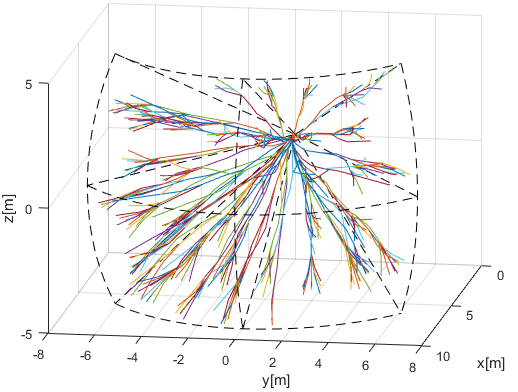
\includegraphics[width=0.7\linewidth]{\FIGDIR/RS003HarmonicReachSetEstimationMethod} 
    \caption{\emph{Harmonic \emph{reach set} approximation}.}
    \label{fig:harmonicReachSetApproximation}
\end{figure}

\paragraph{Pros and Cons:} It can bee seen from example (fig. \ref{fig:harmonicReachSetApproximation}) that \emph{Harmonic Reach Set Approximation Method} (alg. \ref{alg:ExpansionConstraintFunctionForHarmonicReachSet}) generates \emph{smooth evenly spread trajectories}.
    
High smoothness ratio ($\ge 0.9$) is provided, while keeping low node count for UAS systems. The calculation complexity scales linearly with grid size. The upper limit of trajectories is given as follow:

\begin{multline}
    countTrajectories(ReachSet) \le layerCellCount \times spreadLimit \\\times size(Movements)
\end{multline}

\noindent The \emph{upper limit of nodes} is given as follow:

\begin{equation}
    countNodes(ReachSet) \le layerCount \times layerCellCount \times spreadLimit
\end{equation}

\noindent Absence of \emph{High Coverage Ratio} disqualifies \emph{Harmonic Reach Set Approximation} to be used for \emph{Emergency Avoidance}. This type of \emph{Reach Set} is feasible for \emph{Open Space Navigation} or \emph{Controlled Airspace Navigation}. Its low turning rate in contained \emph{Trajectories} are desired for such tasks. 




    	\subsection{ACAS-X like Reach Set Approximation}\label{s:acasReachSet}
\paragraph{Motivation:} The implementation of \emph{ACAS-Xu} behavior in DAA system will  be mandatory for \emph{National Airspace System Integration} in United spaces \cite{shively2018uas}. 

Implementation of ACAS-Xu like behaviour increase usability of approach, if it can be achieved without major concept changes.


\paragraph{Background:} The \emph{ACAS-Xu} system on operational level has been described in \cite{marston2015acas}. The \emph{Policy for Collision Avoidance} proposal has been given in \cite{julian2016policy}.

Some behavioural patterns can be encoded into  \emph{Reach Set}. ACAS-Xu navigation part is basically \emph{Look-up table of Maneuvers for Allowed Separations}.
 
The \emph{Evasive Maneuver} selection process in ACAS-Xu is similar to our approach: \emph{Select most energy efficient maneuver in compliance with space-time constraints}. ACAS-Xu intruder model is similar to our \emph{Body Volume Intersection Model} (app. \ref{s:bodyvolumeIntersection}). The \emph{ACAS-Xu} defines following base separations:

\begin{enumerate}
    \item \emph{Horizontal} - movements on \emph{Horizontal Plane} in \emph{Global Coordinate System}.
    
    \item \emph{Vertical} - movements on \emph{Vertical Plane} in \emph{Global Coordinate System}.
    
\end{enumerate}

\noindent There are allowed custom separations which can be used, for further experimentation: 
\begin{enumerate}
    \item \emph{Slash} - movement on $+45^{\circ}$ \emph{Tilted Plane to Horizontal Plane} in \emph{Global Coordinate System}.
    
    \item \emph{Backslash} - movement on $-45^{\circ}$ \emph{Tilted Plane to Horizontal Plane} in \emph{Global Coordinate System}.
    
\end{enumerate}

\noindent For given \emph{Movement Automaton} implementation (sec. \ref{s:modelMAImplementation}) the separations are given as follow:

\begin{equation}\label{eq:implementedseparations}
    \begin{aligned}
        Horizontal & = \{Straight, Left, Right \}\\
        Vertical & = \{Straight, Up, Down\}\\
        Slash & = \{Straight, UpLeft, DownRight\}\\
        Backslash & = \{Straight, UpRight, DownLeft\}\\
    \end{aligned}
\end{equation}

\noindent For each $Node(\dots,buffer)$ and each \emph{separation} there is a evaluation function $isSeparation$ which decides, if \emph{Trajectory} defined by node buffer is made up only from \emph{Separation} movements.  The function $isSeparation(\dots)$ is defined like:

\begin{equation}\label{eq:isSeparationPredicate}
    isSeparation(buffer,separation) =
    \begin{cases}
        \begin{aligned}
            \forall & movement \in buffer,\\ & movement \in separation
        \end{aligned}&: true\\
        otherwise &: false
    \end{cases}
\end{equation}

\noindent Following \emph{Separation Modes} can be defined with given \emph{separations}:

\begin{enumerate}
    \item \emph{Horizontal} (ACAS-X defined mode) containing \emph{horizontal} separation. 
    
    \item \emph{Vertical} (ACAS-X defined mode) containing \emph{vertical} separation.
    
    \item \emph{Horizontal-Vertical} (ACAS-X defined mode) containing \emph{horizontal, vertical} separations.
    
    \item \emph{Full} (custom defined mode) containing all \emph{Separation Modes}.
    
\end{enumerate}

\begin{note}
    Every separation modes generates 2D trajectories set on \emph{Respective plane}. There is no need for \emph{Tuning parameters} for further \emph{Expansion Constraint}.    
\end{note}

\paragraph{Expansion Constraint Function Implementation} (alg. \ref{alg:ExpansionConstraintFunctionForACASLikeReachSet}) is based on simple principle:
\emph{Select only candidate Nodes which Trajectories have at least one desired Separation Mode}.

\paragraph{Step: Initialization} sets candidate \emph{Nodes} as empty set,  leftover \emph{Nodes} as empty set, and, select all nodes form \emph{stack} which represents \emph{Finishing Trajectories} in working $cell_{i,j,k}$,

\paragraph{Step: Candidate Selection Process} is evaluated for each \emph{test Node} from \emph{passing Node Set}. 

For each \emph{applicable separation}, given as input parameter \emph{separations}, The test function \emph{isSeparation} (eq. \ref{eq:isSeparationPredicate}) is applied:
\begin{enumerate}
    \item If \emph{test Node} trajectory belongs to at least one allowed separation it is added to candidates set.
    \item Else is added to \emph{Leftovers}.
\end{enumerate}

\begin{note}
    \emph{Separation sets} (eq. \ref{eq:implementedseparations}) are not \emph{exclusive sets} in \emph{Movement Automaton} domain. One \emph{Trajectory} contained by Node can belong to multiple \emph{Separations}.    
\end{note}

\begin{algorithm}[H]
\SetKwInOut{Input}{Input}\SetKwInOut{Output}{Output}\SetKwInOut{TuningParameters}{Tuning Parameters}
    \Input{Node[] stack, Cell cell$_{i,j,k}$, Separation[] separations}
    \TuningParameters{$None:\varnothing$}
    \Output{Node[] candidates, Node[] leftovers}
    
    \BlankLine
    \# Initialize structures\;
    Node[] candidates = [], Node[] leftovers=[]\;
    Node[] passing = cell$_{i,j,k}$.getFinishingTrajectories(stack)\;
    
    \BlankLine
    \# Select nodes containing trajectories with usable separations\;
    \For{Node test $\in$ passing}{
        \For{separation $\in$ separations}{
            \BlankLine
            \# Get separations for Node\;
            Separations[] nodeSeparations = test.getSeparations()\;
            \BlankLine
            \# If trajectory given by buffer is on Separation plane\;
            \If{isIn(isSeparation(test.buffer,separation)(\ref{eq:isSeparationPredicate})}{
                candidates.append(test)\;
            }
        }
        \BlankLine
        \# If there was no applicable separation, throw Node away\;
        \If{test $\not\in$ candidates}{
            leftovers.append(test)\;
        }
    }
    \BlankLine
    \# Return results\;
    \Return{[candidates,leftovers]}
    
    \caption{Expansion Constraint function for \emph{ACAS-like Reach Set Approximation}}
    \label{alg:ExpansionConstraintFunctionForACASLikeReachSet}    
\end{algorithm}

\paragraph{Example:} for \emph{Avoidance Grid} with \emph{Distance 10 m}, \emph{Layer count 10}, \emph{Horizontal range $[-45^\circ,+45^\circ]$}, \emph{Horizontal Cell Count 7}, \emph{Vertical range $[-30^\circ,+30^\circ]$}, and \emph{Vertical Cell Count 5}. Is given in (fig. \ref{fig:acasLikeReachSetVariousSeparationMode}). The UAS is at \emph{Back-side} of \emph{Figure} (initial state is at all \emph{Trajectory Origins}). The \emph{black dashed line} marks \emph{Avoidance Grid} space boundary. Each trajectory has its own color and ends at \emph{Front-side} of \emph{Avoidance Grid Boundary}.

\emph{Full} separation mode given in (fig. \ref{fig:acasLikeReachSetFull}). \emph{Horizontal-Vertical} separation mode, used in original \emph{ACAS-Xu} testing \cite{marston2015acas}, given in (fig. \ref{fig:acasLikeReachSetHorizontalVertical}). \emph{Horizontal} separation mode given in (fig. \ref{fig:acasLikeReachSetHorizontalOnly}) is usually used by planes. \emph{Vertical} separation mode given in (fig. \ref{fig:acasLikeReachSetVerticalOnly}) is usually used by copters.

\begin{figure}[H]
	\centering
    \begin{subfigure}{0.48\textwidth}
        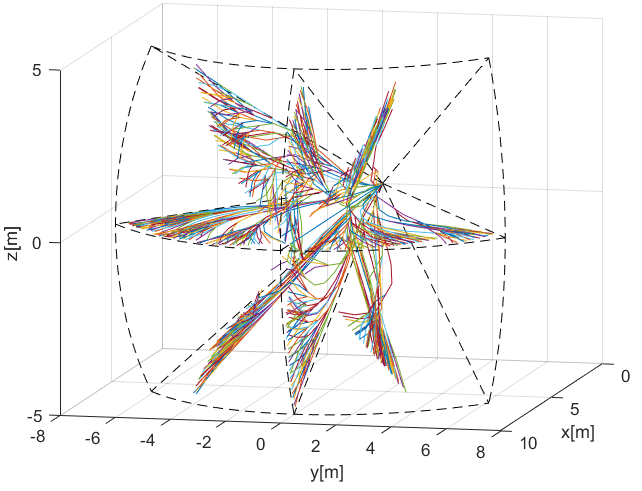
\includegraphics[width=0.9\linewidth]{\FIGDIR/RS005ACASLikeReachSetEstimationMethodFull}
        \caption{Full.}
        \label{fig:acasLikeReachSetFull}
    \end{subfigure}
    \begin{subfigure}{0.48\textwidth}
        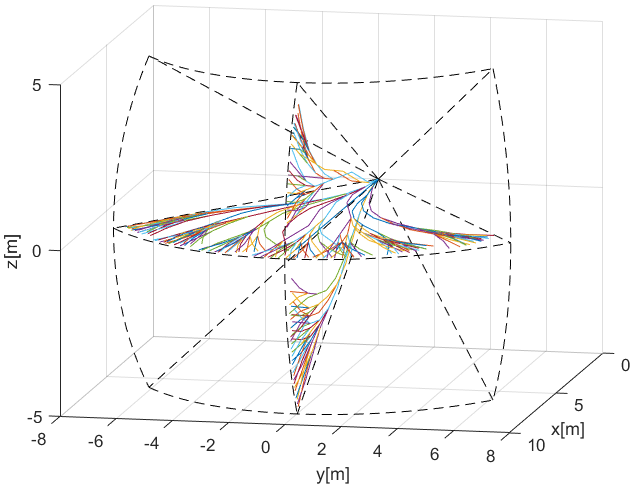
\includegraphics[width=0.9\linewidth]{\FIGDIR/RS006ACASLikeReachSetEstimationMethodHorizontalVertical} 
        \caption{Horizontal-Vertical.}
        \label{fig:acasLikeReachSetHorizontalVertical}
    \end{subfigure}
    \\
    \begin{subfigure}{0.48\textwidth}
        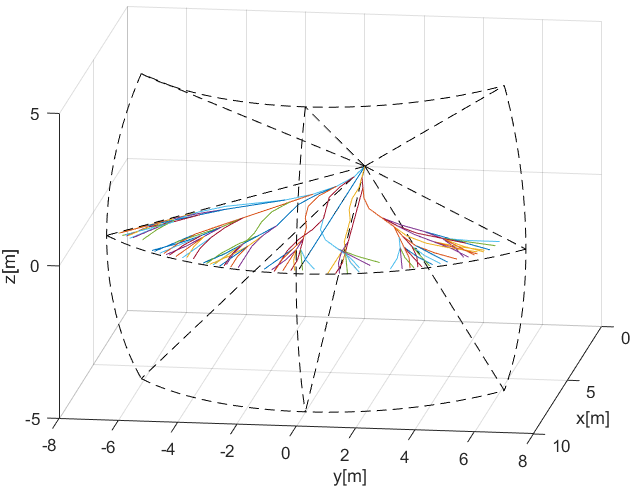
\includegraphics[width=0.9\linewidth]{\FIGDIR/RS008ACASLikeReachSetEstimationMethodHorizontal} 
        \caption{Horizontal.}
        \label{fig:acasLikeReachSetHorizontalOnly}
    \end{subfigure}
    \begin{subfigure}{0.48\textwidth}
        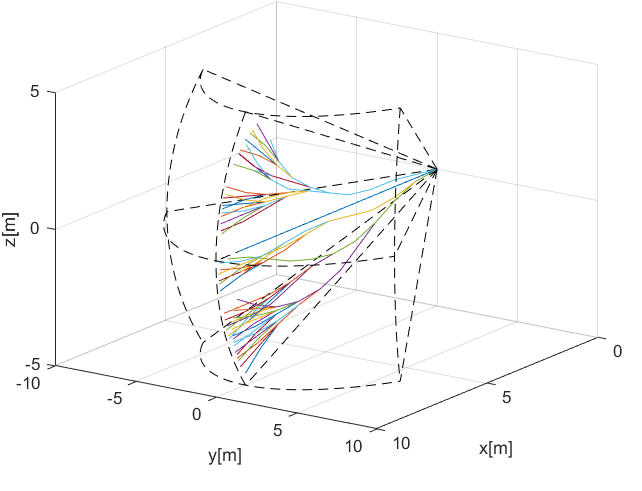
\includegraphics[width=0.9\linewidth]{\FIGDIR/RS009CASLikeReachSetEstimationMethodVertical} 
        \caption{Vertical.}
        \label{fig:acasLikeReachSetVerticalOnly}
    \end{subfigure}
    \caption{ACAS-X imitation \emph{reach set} approximation for various \emph{separation modes}. }
    \label{fig:acasLikeReachSetVariousSeparationMode}
\end{figure}

\paragraph{Pros and Cons:} It can be seen from examples (fig. \ref{fig:acasLikeReachSetVariousSeparationMode}) that \emph{ACAS-like Reach Set Approximation Method} (alg. \ref{alg:ExpansionConstraintFunctionForACASLikeReachSet}) generates full reach set for 2D plane located in 3D space. 

The \emph{Reach Set} contains trajectories with \emph{high coverage ratio} and \emph{high smoothness rating} for selected 2D separation plane. Overall performance compared to full 3D reach sets (sec. \ref{s:chaoticReachSet}, \ref{s:harmonicReachSet} \ref{s:combinedReachSet}) is poor. 

The \emph{node} and \emph{trajectory} count boundary was not implemented. It is common knowledge that \emph{2D} avoidance sets does not require scaling \cite{marston2015acas}. Otherwise trajectory footprint mechanism like in \emph{Harmonic Reach Set Approximation} (alg. \ref{alg:ExpansionConstraintFunctionForHarmonicReachSet}) can be introduced.

This reach set implements \emph{Planar-Separation} as native feature, it can be used for both \emph{navigation} and \emph{avoidance} tasks in \emph{Controlled Airspace}. For \emph{Non-controlled Airspace} there are far more superior \emph{Combined Reach Set} (sec. \ref{s:combinedReachSet}).

    	
\subsection{(R) Chaotic Reach set}\label{s:chaoticReachSet}

\paragraph{Motivation:} Design of calculation method for \emph{Reach Set Approximation} guarantying high \emph{Maneuverability}.

\paragraph{Background:}There is \emph{Coverage Ratio} property of \emph{Reach Set} (def. \ref{def:coverageRatio}). It has been shown that creating \emph{Reach Set} via \emph{greedy approach} is not feasible due the \emph{Scaling Factor}.  \emph{Contracted Expansion} (sec. \ref{s:constrainedTrajectoryExpansion}) is enabling to apply selection criteria while building \emph{Reach Set} in given \emph{Cell}. 

The \emph{Cell} $cell_{i,j,k}$ has a center and walls from UAS viewpoint: front wall , back wall (for $layer > 1$), top wall, left wall, right wall, bottom wall. It is expected that trajectory leading close to one cell walls will continue to different cell, increasing chance to obtain more \emph{Unique Footprints}. 

\paragraph{Expansion Constraint Function Implementation} (alg. \ref{alg:ExpansionConstraintFunctionForChaoticReachSet}) is based on simple principle: \emph{Select candidate Nodes which are  closest to outer walls of Cell, with unique footprint}.

\paragraph{Tuning Parameters}: \emph{Proximity to Cell outer wall} gives good chances to break into other rows or columns in \emph{Avoidance Grid}. \emph{Unique footprint} guarantees future \emph{Unique Footprint} after appending Trajectory by \emph{Movement application}. 
\begin{enumerate}
    \item \emph{Considered Footprint Length} - how much last cells in footprint should be considered in unique path track, minimal value 1, default value 3, maximal value $\infty$. If you want to generate non redundant trajectories use $\infty$, it will consider full footprint.
    
    \item \emph{Spread Limit} - upper limit of candidates which are going to be select for further expansion, minimal value 1, default value \emph{Count of unique Moves in Movement set}, maximal value $\infty$. If more than default values is selected the algorithm will generate \emph{redundant trajectories}. If less is selected then some trajectories are omitted and \emph{Coverage Rate} decreases sharply. 
\end{enumerate}


\paragraph{Step: Initialization} initialization of \emph{candidate} array (return value), \emph{leftovers} array (return Value). Node array \emph{passing} is populated with \emph{Nodes} which represents \emph{end node of Trajectory} and the tip of \emph{trajectory is constrained in \emph{cell}$_{i,j,k}$}.

\paragraph{Step: Evaluate best trajectories with unique Footprints} following steps are executed:
\begin{enumerate}
    \item \emph{Best Performance Map} is created with \emph{footprint} as key set element to ensure footprint uniqueness.
    \item \emph{Wall distance} for \emph{test node} is calculated as a closest trajectory portion distance to \emph{top, bottom, left, right} wall of cell $cell_{i,j,k}$
    \item \emph{Footprint} for \emph{test node} is created with maximal length given by \emph{Footprint Length} tuning parameter.
    \item \emph{Existence and Performance Test} is executed to ensure that best performing node is selected. If there is not key entry in the \emph{Best Performance Map}, then new entry for \emph{Test Node} is created. If there is key entry, the performance of \emph{Old Node} and \emph{Test Node} is compared and better is stored.
\end{enumerate}

\paragraph{Step: Select candidates} is executed on \emph{Best Performance Map} records using  \emph{Wall distance} as pivot parameter, ordering by closest proximity and limited by \emph{Search Limit} tuning parameter. The \emph{Leftovers} are difference set between \emph{Passing Nodes} and \emph{Candidate Nodes}. 

\begin{algorithm}[H]
    \SetKwInOut{Input}{Input}\SetKwInOut{Output}{Output}\SetKwInOut{TuningParameters}{Tuning Parameters}
    \Input{Node[] stack, Cell cell$_{i,j,k}$}
    \TuningParameters{int$^+$ footprintLength, int$^+$ spreadLimit}
    \Output{Node[] candidates, Node[] leftovers}
    
    \BlankLine
    \# Initialize structures\;
    Node[] candidates = [], Node[] leftovers=[]\;
    Node[] passing = cell$_{i,j,k}$.getFinishingTrajectories(stack)\;
    
    \BlankLine
    \# Select best performing trajectories with unique footprint\;
    Map$<$Footprint,Node$>$  bestPerformanceMap\;
    \For{Node test $\in$ passing}{
        wallDistance= test.minimalDistanceToWall(cell$_{i,j,k}$)]\;
        footPrint = test.getFootprint(lastCells = footprintLength)\;
        \eIf{bestPerformanceMap.contains(footPrint)}{
            old = bestPerformanceMap.getByKey(footprint)\;
            oldPerformance= old.minimalDistanceToWall(cell$_{i,j,k}$)\;
            \If{oldPerformance $>$ wallDistance}{
                bestPerformanceMap.setByKey(footprint,test)\;         
            }
        }{
            bestPerformanceMap.setByKey(footprint,test)\;
        }
    }
    
    \BlankLine
    \# Select best performing nodes up to \emph{spreadLimit} count\;
    candidates = bestPerformanceMap.select(count = spreadLimit).orderBy('wallDistance','Ascending')\;
    leftovers = passing - candidates\;
    \Return{[candidates,leftovers]}
    
    
    \caption{Expansion Constraint function for \emph{Chaotic Reach Set Approximation}}
    \label{alg:ExpansionConstraintFunctionForChaoticReachSet}
\end{algorithm}

\paragraph{Example:} for \emph{Avoidance Grid} with \emph{Distance 10 m}, \emph{Layer count 10}, \emph{Horizontal range $[-45^\circ,+45^\circ]$}, \emph{Horizontal Cell Count 7}, \emph{Vertical range $[-30^\circ,+30^\circ]$}, and \emph{Vertical Cell Count 5}. Is given in (fig. \ref{fig:chaoticReachSetApproximation}). The UAS is at \emph{Back-side} of \emph{Figure} (initial state is at all \emph{Trajectory Origins}). The \emph{black dashed line} marks \emph{Avoidance Grid} space boundary. Each trajectory has its own color and ends at \emph{Front-side} of \emph{Avoidance Grid Boundary}.


\begin{figure}[H]
    \centering
    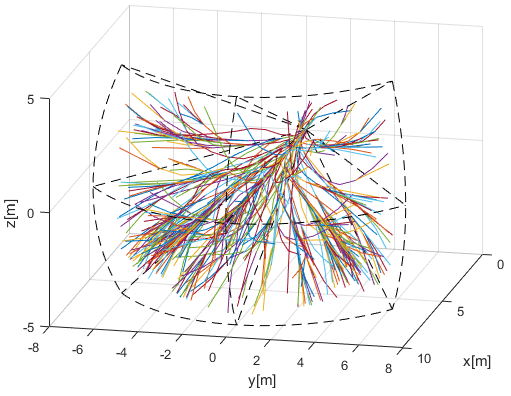
\includegraphics[width=0.7\linewidth]{\FIGDIR/RS002ChaoticReachSetEstimationMethod} 
    \caption{\emph{Chaotic \emph{reach set} approximation}.}
    \label{fig:chaoticReachSetApproximation}
\end{figure}

\paragraph{Pros and Cons:} It can be seen from example (fig. \ref{fig:chaoticReachSetApproximation}) that \emph{Chaotic Reach Set Approximation Method} (alg. \ref{alg:ExpansionConstraintFunctionForChaoticReachSet}) generates a lot of \emph{turning} and \emph{shaky} \emph{trajectories}. 

\emph{High Coverage Ratio} ($\sim 0.9$) is provided, while keeping \emph{medium node count}. The calculation complexity scales linearly with grid size. The \emph{upper limit of trajectories} is given as follow:

\begin{multline}
    countTrajectories(ReachSet) \le layerCellCount \times spreadLimit\\ \times size(Movements)
\end{multline}

\noindent The \emph{upper limit of nodes} is given as follow:
    
\begin{multline}
    countNodes(ReachSet) \le layerCount \times  layerCellCount  \\
    \times size(Movements) \times spreadLimit  
\end{multline}

\noindent\emph{Absence} of \emph{Smooth Trajectories} disqualifies \emph{Chaotic Reach Set Approximation} to be used for \emph{Navigation}. This type of reach set is feasible for \emph{Avoidance}, because it contains variety of maneuvers.


\subsection{(R) Harmonic Reach set}\label{s:harmonicReachSet}

\paragraph{Motivation:} Imagine having an \emph{Avoidance Grid} like (fig. \ref{fig:LidarSpaceSegmentation}). There is a need of \emph{Reach Set Approximation} which will have \emph{Smooth Trajectories} (def. \ref{def:SmoothnessRatingForTrajectory}) going nearby $cell$ centers.

\paragraph{Background:} The \emph{Smoothness Rating for Trajectory} (def. \ref{def:SmoothnessRatingForTrajectory}) uses two distinct sets \emph{Smooth Movements} and \emph{Chaotic Movements} (eq. \ref{eq:ChaoticSmoothMovementSetDefinition}) which are defined for our \emph{Movement Automaton}  (sec. \ref{s:modelMAImplementation}) like follow:

\begin{equation}
    \begin{aligned}
    Smooth Movements &= \{Straight\} \\
    Chaotic Movements &= Movements - Smooth Movements\\
    \end{aligned}
\end{equation}

\emph{Smooth Movements} contains only \emph{Straight} movement, because others are considered as extreme turning movements. \emph{Smooth Movements} should contain only direct flight movements or slight heading correction. \emph{Chaotic Movements} set is supplement of \emph{Movement Automaton`s Movement Set}. 

The \emph{Avoidance Grid} (fig. \ref{fig:LidarSpaceSegmentation}) cell centers for fixed indexes $j_{fix}$, $k_{fix}$ are linearly aligned with \emph{initial state}. That means that  cell centers of cells $cell_{1,j_{fix},k_{fix}},\dots, cell_{i,j_{fix},k_{fix}}$, where $i$ is count of \emph{layers} lies on one line.  If the trajectory can achieve \emph{cell center} on some \emph{layer} only minor trajectory corrections are required to stay on given line. This type of trajectory gives us following advantages:
\begin{enumerate}
    \item\emph{Minimal steering at beginning} - the minimal steering is advantageous in \emph{Controlled Airspace} because is diminishing the amount of communication to \emph{UTM Service}.
    
    \item\emph{Additional safe space in Linear segment} - once the \emph{center of cell} is reached, \emph{Trajectory} sticks to line between cell centers. Each point on this line has \emph{maximal distance} to outer walls of cell. This gives us extra space given as minimum of distance between \emph{UAS position} and \emph{Outer cell walls}.
\end{enumerate}

\paragraph{Expansion Constraint Function Implementation} (alg. \ref{alg:ExpansionConstraintFunctionForHarmonicReachSet}) is based on simple principle: \emph{Select candidate Nodes  which are closest to Cell center, with unique footprint}.

\begin{note}
    \emph{Cell center} can be closely reached by \emph{smooth movement} from previous cell or \emph{chaotic movement} from neighbouring cell from current or previous layer. These trajectories are usually equivalent in \emph{Smoothness}.
\end{note}

\paragraph{Tuning Parameter:} \emph{Proximity to Cell Center} gives a good chance to keep trajectory smooth or \emph{smooth after one correction maneuver}. It has been mentioned that \emph{Cell Center} can be reached by various trajectories. In this method full footprint length is always considered, therefore only one tuning parameter can be offered:
\begin{enumerate}
    \item \emph{Spread Limit} - upper limit of candidates which are going to be selected for further expansion, minimal value 1, default value \emph{Count of unique Moves in Movement set}, maximal value $\infty$. If maximal value $\infty$ is selected, algorithm will generate skeleton of \emph{Reach Set} with full Coverage and with the smoothest \emph{Trajectories}.
\end{enumerate}

\paragraph{Step: Initialization} sets candidate \emph{Nodes} as empty set, leftover \emph{Nodes} as empty set. and selects all \emph{Nodes} from \emph{Stack} which represents  \emph{Finishing Trajectories} in working cell $cell_{i,j,k}$.

\paragraph{Step: Evaluate smoothest trajectories with unique Footprints} is implemented as \emph{multi-criteria filtration}. 

\emph{First criterion} is \emph{distance to Cell Center} which is penalized by trajectory \emph{smoothness rate} implemented in method \emph{Node.getPerformance(Cell $cell_{i,j,k}$)} defined as follow.

\begin{equation}
    getPerformance(Node,Cell) = \frac{distance(Node.Trajectory,Cell.Center)}{SmoothnessRate(Node.Trajectory)}
\end{equation}

\noindent Distance of \emph{Trajectory} is \emph{enumerator}, because its considered as \emph{base value} and is defined in interval $[0,maximalWallDistance]$. The \emph{Smoothness Rate} is in denominator, because it is a penalization coefficient defined in interval $[0,1]$. 

\emph{Second criterion} is \emph{trajectory uniqueness} This is provided by \emph{Best Performance Map}, where best performing \emph{Node} belongs to one unique \emph{trajectory footprint}. The implementation is identical to \emph{chaotic reach set expansion} (alg. \ref{alg:ExpansionConstraintFunctionForChaoticReachSet}).

\paragraph{Step: Select candidates} is executed  on \emph{Best Performance Map} records using \emph{Penalized Cell Center Distance} as pivot parameter, ordered in ascending order and limited by \emph{Spread Limit} tuning parameter. The \emph{Leftovers} are difference set between \emph{Passing Nodes} and \emph{Candidate Nodes}.

\begin{algorithm}[H]
\SetKwInOut{Input}{Input}\SetKwInOut{Output}{Output}\SetKwInOut{TuningParameters}{Tuning Parameters}
    \Input{Node[] stack, Cell cell$_{i,j,k}$}
    \TuningParameters{int$^+$ spreadLimit}
    \Output{Node[] candidates, Node[] leftovers}
    
    \BlankLine
    \# Initialize structures\;
    Node[] candidates = [], Node[] leftovers=[]\;
    Node[] passing = cell$_{i,j,k}$.getFinishingTrajectories(stack)\;
    
    \BlankLine
    \# Select unique smoothest trajectories\;
    Map$<$Buffer,Node$>$  bestPerformanceMap\;
    \For{Node test $\in$ passing}{
        centerDistance= test.getPerformance(cell$_{i,j,k}$)]\;
        footPrint = test.getFootprint()\;
        \eIf{bestPerformanceMap.contains(footPrint)}{
            old = bestPerformanceMap.getByKey(footprint)\;
            oldPerformance= old.getPerformance(cell$_{i,j,k}$)\;
            \If{oldPerformance $>$ centerDistance}{
                bestPerformanceMap.setByKey(footprint,test)\;         
            }
        }{
            bestPerformanceMap.setByKey(footprint,test)\;
        }
    }
    
    \BlankLine
    \# Select best performing nodes up to \emph{spreadLimit} count\;
    candidates = bestPerformanceMap.select(count = spreadLimit).orderBy('cellCenterDistance','Ascending')\;
    leftovers = passing - candidates\;
    \Return{[candidates,leftovers]}
    
    
    \caption{Expansion Constraint function for \emph{Harmonic Reach Set Approximation}}
    \label{alg:ExpansionConstraintFunctionForHarmonicReachSet}    
\end{algorithm}


\paragraph{Example:} for \emph{Avoidance Grid} with \emph{Distance 10 m}, \emph{Layer count 10}, \emph{Horizontal range $[-45^\circ,+45^\circ]$}, \emph{Horizontal Cell Count 7}, \emph{Vertical range $[-30^\circ,+30^\circ]$}, and \emph{Vertical Cell Count 5}. Is given in (fig. \ref{fig:harmonicReachSetApproximation}). The UAS is at \emph{Back-side} of \emph{Figure} (initial state is at all \emph{Trajectory Origins}). The \emph{black dashed line} marks \emph{Avoidance Grid} space boundary. Each trajectory has its own color and ends at \emph{Front-side} of \emph{Avoidance Grid Boundary}. The \emph{Spread Limit} in this case was set to $9$ which is \emph{Size of the Movement Set}.

\begin{note}
    Please note \emph{Trajectories} are organized in bundles going around \emph{Cell Centers smoothly}. Most of the steering maneuvers are executed at the \emph{beginning} of \emph{Avoidance Grid}.
\end{note}

\begin{figure}[H]
    \centering
    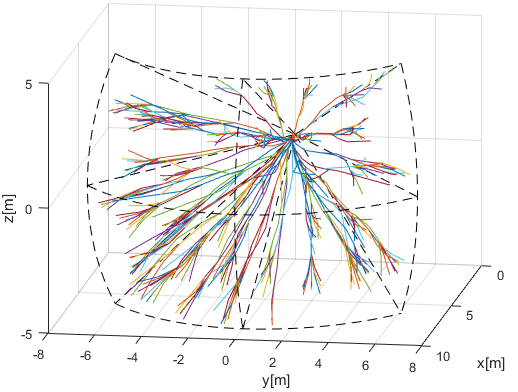
\includegraphics[width=0.7\linewidth]{\FIGDIR/RS003HarmonicReachSetEstimationMethod} 
    \caption{\emph{Harmonic \emph{reach set} approximation}.}
    \label{fig:harmonicReachSetApproximation}
\end{figure}

\paragraph{Pros and Cons:} It can bee seen from example (fig. \ref{fig:harmonicReachSetApproximation}) that \emph{Harmonic Reach Set Approximation Method} (alg. \ref{alg:ExpansionConstraintFunctionForHarmonicReachSet}) generates \emph{smooth evenly spread trajectories}.
    
High smoothness ratio ($\ge 0.9$) is provided, while keeping low node count for UAS systems. The calculation complexity scales linearly with grid size. The upper limit of trajectories is given as follow:

\begin{multline}
    countTrajectories(ReachSet) \le layerCellCount \times spreadLimit \\\times size(Movements)
\end{multline}

\noindent The \emph{upper limit of nodes} is given as follow:

\begin{equation}
    countNodes(ReachSet) \le layerCount \times layerCellCount \times spreadLimit
\end{equation}

\noindent Absence of \emph{High Coverage Ratio} disqualifies \emph{Harmonic Reach Set Approximation} to be used for \emph{Emergency Avoidance}. This type of \emph{Reach Set} is feasible for \emph{Open Space Navigation} or \emph{Controlled Airspace Navigation}. Its low turning rate in contained \emph{Trajectories} are desired for such tasks. 



\subsection{(R) Combined Reach set}\label{s:combinedReachSet}
\paragraph{Motivation:} Harmonic reach set (sec. \ref{s:harmonicReachSet}) is \emph{efficient} for \emph{Navigation in \emph{Controlled Airspace}}. Chaotic reach set (sec. \ref{s:chaoticReachSet}) is good for \emph{Emergency avoidance}. The need to differentiation between \emph{Navigation} and \emph{Emergency Avoidance} mode is necessary in \emph{Controlled Airspace}. but not in \emph{Non-controlled Airspace}. The combination of \emph{Harmonic} and \emph{Chaotic} reach sets is obvious solution. 

\emph{Automatic mode switch} can be provided by combination of \emph{Navigation Reach Set} and \emph{Avoidance Reach Set} with elevated cost function. Overall having a method to merge multiple trees would be beneficial.

\paragraph{Background:} If two \emph{Reach Set Approximation} were calculated for same \emph{Avoidance Grid} and \emph{Initial State}, using same \emph{Movement Automaton} and \emph{UAS model} are possible to merge. 

The \emph{Reach Set Approximation} is \emph{tree} with \emph{Root Node} in \emph{initail state} with movement buffer = $\varnothing$. The \emph{movement buffer} in each node can be used as \emph{route trace} during merging procedure. The example two reach set merge can be given as follow, where only \emph{latest} applied movement is taken into account.

\begin{equation}\label{eq:mergeTreeFunctionExample}
    \left[
    \begin{aligned}
    \texttt{Fi}&\texttt{rst Reach Set}\\
        &\varnothing \to 
            \left<
                \begin{aligned}
                    &left \to \left<
                                \begin{aligned}
                                    &left\\
                                    &right
                                \end{aligned}
                              \right.\\
                    &\varnothing\\
                \end{aligned}
             \right.\\ 
    \texttt{Se}&\texttt{cond Reach Set}\\
        &\varnothing \to 
            \left<
                \begin{aligned}
                    & \varnothing \\
                    & right \to \left< 
                                    \begin{aligned}
                                        &left\\
                                        &right
                                    \end{aligned}
                                \right.\\
                \end{aligned}
            \right.\\
    \end{aligned}
    \right]
    \to
    \left[
    \begin{aligned}
    \texttt{Co}&\texttt{mbined Reach Set}\\
    &\varnothing\to
        \left< 
            \begin{aligned}
                &left &\to   \left< 
                                \begin{aligned}
                                    &left\\
                                    &right
                                \end{aligned}    
                            \right.\\
                &right &\to   \left< 
                                \begin{aligned}
                                    &left\\
                                    &right
                                \end{aligned}    
                            \right.\\
            \end{aligned}    
        \right.
    \end{aligned}
    \right]
\end{equation}

\emph{First Reach Set} contains two trajectories given by buffers \emph{\{left,left\}} and \emph{\{left,right\}}. \emph{Second Reach Set} contains two trajectories given by buffers \emph{\{right,left\}} and \emph{\{right,right\}}. The \emph{Combined Reach Set} contains all four trajectories.

\begin{note}
    The combined tree \cite{o1996log} does not need to have combined amount of original \emph{Reach Sets} trajectories. There can be \emph{Duplicity} which means that any bounded property like \emph{Cost} must be \emph{calculated} again.
\end{note}

\paragraph{Combined Reach Set Calculation Function} (alg. \ref{alg:ReachSetMerge}) is implemented as function $Node combinedReachSet(\dots)$ which takes root Node with \emph{initial State}, \emph{Avoidance Grid} and respective parameters for each calculation method. \emph{Harmonic spread} for \emph{Harmonic Reach set calculation} and \emph{Chaotic Spread}, \emph{Footprint Length} for \emph{Chaotic Reach set calculation}.

\emph{Separate Reach Sets} are calculated using \emph{Wave-front propagation} (alg. \ref{alg:Wavefront Propagation}) using respective \emph{Constrained Expansion} functions for \emph{Harmonic} (alg. \ref{alg:ExpansionConstraintFunctionForHarmonicReachSet}) and \emph{Chaotic} (alg. \ref{alg:ExpansionConstraintFunctionForChaoticReachSet}) reach sets.

\emph{Combined Reach Set} is created using \emph{Node mergeTree($\dots$)} function. Because different cost function or \emph{Bounded Parameters Calculation} may be applied on \emph{Original Reach Sets}.

\emph{Cost} for \emph{each node} needs to be recalculated due to original reach sets disparity. Function \emph{combined.applyCostFunction()} will recalculate the new cost for each node. 

The Goal is to have penalization for \emph{Chaotic behaviour}, implementation of \emph{Automatic Mode Switch} can be done like follows:
\begin{enumerate}
    \item \emph{Calculate Normal Cost} for Node $Cost(Node)$ for associated trajectory:\\ $Cost(Node.Trajectory)$.
    \item \emph{Calculate Penalization for \emph{Chaotic Behaviour}}, calculate \emph{Smoothness Rating for Trajectory} (def. \ref{def:SmoothnessRatingForTrajectory}) in interval $[0,1]$, introduce penalization with base $100 \%$.
\end{enumerate}

The final $Cost(Node)$ function is applied on each \emph{Combined Reach Set Node} and look like follows:

\begin{multline}
    Cost(Node) = Cost(Node.Trajectory) \times\dots\\\dots\times \left(1+ \left(1-SmoothnessRate(N ode.T rajectory)\right)\right)
\end{multline}

\paragraph{Merge Tree Function} $mergeTree(\dots)$ implements \emph{Outer Join} operation on two trees. Example was given in (eq. \ref{eq:mergeTreeFunctionExample}).
Function is applied on \emph{root Node} iterating over \emph{Movements in Movement Set}, because \emph{Movement is pivot}.

\begin{algorithm}[H]
    \SetKwProg{Fn}{}{}{}\SetKwFunction{FRecurs}{Node mergeTree}
    \SetKwProg{Fn}{}{}{}\SetKwFunction{FMain}{Node combinedReachSet}
    
    \BlankLine
    \# Tree merge function\;
    \Fn(){\FRecurs{Node firstNode, Node secondNode}}{
        \BlankLine
        \# Try to copy reference node or return null\;
        Node referenceNode = (firstNode?:(secondNode?: return null))\;
        Node merged =  new Node(referenceNode)\;
        merged.leafs= []\;
        \BlankLine
        \# Try to fetch movement nodes if exist in any sub tree\;
        \For{movement $\in$ Movements}{
            firstLeaf = firstNode.getLeafFor(movement)\;
            secondLeaf = secondNode.getLeafFor(movement)\;
            newLeaf = mergeTree(firstLeaf,secondLeaf)\;
            \If{newLeaf $\sim = $ null}{
                merged.leafs.append(newLeaf)\;
            }
        }
        \Return{merged}
    }{}
    
    \BlankLine
    \# Combined Reach Set calculation function\;
    \Fn(){\FMain{Node root, AvoidanceGrid grid,int$^+$ chaoticSpread, int$^+$ harmonicSpread, int$^+$ footprintLength}}{
        Node chaotic = chaoticReachSet(root,grid, footprintLength,chaoticSpread)\;
        Node harmonic = harmonicReachSet(root,grid, harmonicSpread)\;
        Node combined = mergeTree(chaotic,harmonic)\;
        combined.applyCostFunction()\;
        \Return{combined}
    }

    
    \caption{Reach Set Merge Function and Combined Reach Set calculation}
    \label{alg:ReachSetMerge}
\end{algorithm}

\paragraph{Example:} for \emph{Avoidance Grid} with \emph{Distance 10 m}, \emph{Layer count 10}, \emph{Horizontal range $[-45^\circ,+45^\circ]$}, \emph{Horizontal Cell Count 7}, \emph{Vertical range $[-30^\circ,+30^\circ]$}, and \emph{Vertical Cell Count 5}. Is given in (fig. \ref{fig:combinedReachSetApproximation}). The UAS is at \emph{Back-side} of \emph{Figure} (initial state is at all \emph{Trajectory Origins}). The \emph{black dashed line} marks \emph{Avoidance Grid} space boundary. Each trajectory has its own color and ends at \emph{Front-side} of \emph{Avoidance Grid Boundary}. The \emph{Chaotic Spread} was set to 8, \emph{Footprint Length} to 3 and \emph{Harmonic Spread} to 1.

\begin{note}
    Notice there are typical trajectories from both \emph{Harmonic} (fig. \ref{fig:harmonicReachSetApproximation}) and \emph{Chaotic} (fig. \ref{fig:chaoticReachSetApproximation}) \emph{Reach Set Approximations}.
\end{note}

\begin{figure}[H]
    \centering
    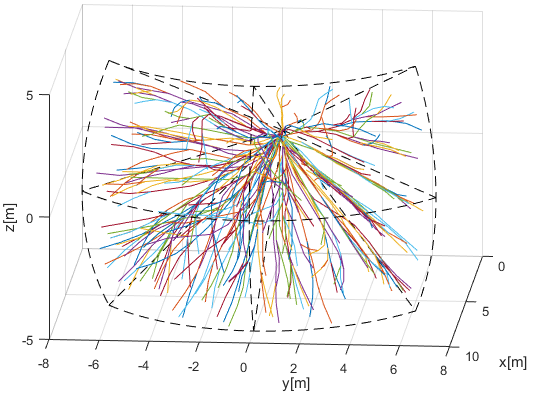
\includegraphics[width=0.7\linewidth]{\FIGDIR/RS004CombinedReachSetEstimationMethod} 
    \caption{\emph{Combined \emph{reach set} approximation}.}
    \label{fig:combinedReachSetApproximation}
\end{figure}


\paragraph{Pros and Cons:} It can bee seen from example (fig. \ref{fig:combinedReachSetApproximation}) that \emph{Combined Reach Set Approximation} (alg. \ref{alg:ReachSetMerge}) contains both types of maneuvers. \emph{Cheaper Smooth} for navigation and \emph{More Expensive Chaotic} for \emph{Emergency Avoidance}. The upper limit of trajectories is given as follow:

\begin{multline}
    countTrajectories(ReachSet) \le countTrajectories(Chaotic) \\+ countTrajectories(Harmonic)
\end{multline}

\noindent The \emph{upper limit of nodes} is given as follow:

\begin{equation}
    countNodes(ReachSet) \le countNodes(Chaotic)+ countNodes(Harmonic)
\end{equation}

\noindent \emph{Harmonic Reach Set} is ideal for \emph{Non-controlled Airspace} missions, because it contains \emph{Automatic Mode Switch} between \emph{Navigation} and \emph{Emergency Avoidance}.


\subsection{(R) ACAS-X like Reach set}\label{s:acasReachSet}
\paragraph{Motivation:} The implementation of \emph{ACAS-Xu} behavior in DAA system will  be mandatory for \emph{National Airspace System Integration} in United spaces \cite{shively2018uas}. 

Implementation of ACAS-Xu like behaviour increase usability of approach, if it can be achieved without major concept changes.


\paragraph{Background:} The \emph{ACAS-Xu} system on operational level has been described in \cite{marston2015acas}. The \emph{Policy for Collision Avoidance} proposal has been given in \cite{julian2016policy}.

Some behavioural patterns can be encoded into  \emph{Reach Set}. ACAS-Xu navigation part is basically \emph{Look-up table of Maneuvers for Allowed Separations}.
 
The \emph{Evasive Maneuver} selection process in ACAS-Xu is similar to our approach: \emph{Select most energy efficient maneuver in compliance with space-time constraints}. ACAS-Xu intruder model is similar to our \emph{Body Volume Intersection Model} (sec. \ref{s:bodyvolumeIntersection}). The \emph{ACAS-Xu} defines following base separations:

\begin{enumerate}
    \item \emph{Horizontal} - movements on \emph{Horizontal Plane} in \emph{Global Coordinate System}.
    
    \item \emph{Vertical} - movements on \emph{Vertical Plane} in \emph{Global Coordinate System}.
    
\end{enumerate}

\noindent There are allowed custom separations which can be used, for further experimentation: 
\begin{enumerate}
    \item \emph{Slash} - movement on $+45^{\circ}$ \emph{Tilted Plane to Horizontal Plane} in \emph{Global Coordinate System}.
    
    \item \emph{Backslash} - movement on $-45^{\circ}$ \emph{Tilted Plane to Horizontal Plane} in \emph{Global Coordinate System}.
    
\end{enumerate}

\noindent For given \emph{Movement Automaton} implementation (sec. \ref{s:modelMAImplementation}) the separations are given as follow:

\begin{equation}\label{eq:implementedseparations}
    \begin{aligned}
        Horizontal & = \{Straight, Left, Right \}\\
        Vertical & = \{Straight, Up, Down\}\\
        Slash & = \{Straight, UpLeft, DownRight\}\\
        Backslash & = \{Straight, UpRight, DownLeft\}\\
    \end{aligned}
\end{equation}

\noindent For each $Node(\dots,buffer)$ and each \emph{separation} there is a evaluation function $isSeparation$ which decides, if \emph{Trajectory} defined by node buffer is made up only from \emph{Separation} movements.  The function $isSeparation(\dots)$ is defined like:

\begin{equation}\label{eq:isSeparationPredicate}
    isSeparation(buffer,separation) =
    \begin{cases}
        \begin{aligned}
            \forall & movement \in buffer,\\ & movement \in separation
        \end{aligned}&: true\\
        otherwise &: false
    \end{cases}
\end{equation}

Following \emph{Separation Modes} can be defined with given \emph{separations}:

\begin{enumerate}
    \item \emph{Horizontal} (ACAS-X defined mode) containing \emph{horizontal} separation. 
    
    \item \emph{Vertical} (ACAS-X defined mode) containing \emph{vertical} separation.
    
    \item \emph{Horizontal-Vertical} (ACAS-X defined mode) containing \emph{horizontal, vertical} separations.
    
    \item \emph{Full} (custom defined mode) containing all \emph{Separation Modes}.
    
\end{enumerate}

\begin{note}
    Every separation modes generates 2D trajectories set on \emph{Respective plane}. There is no need for \emph{Tuning parameters} for further \emph{Expansion Constraint}.    
\end{note}

\paragraph{Expansion Constraint Function Implementation} (alg. \ref{alg:ExpansionConstraintFunctionForACASLikeReachSet}) is based on simple principle:
\emph{Select only candidate Nodes which Trajectories have at least one desired Separation Mode}.

\paragraph{Step: Initialization} sets candidate \emph{Nodes} as empty set,  leftover \emph{Nodes} as empty set, and, select all nodes form \emph{stack} which represents \emph{Finishing Trajectories} in working $cell_{i,j,k}$,

\paragraph{Step: Candidate Selection Process} is evaluated for each \emph{test Node} from \emph{passing Node Set}. 

For each \emph{applicable separation}, given as input parameter \emph{separations}, The test function \emph{isSeparation} (eq. \ref{eq:isSeparationPredicate}) is applied:
\begin{enumerate}
    \item If \emph{test Node} trajectory belongs to at least one allowed separation it is added to candidates set.
    \item Else is added to \emph{Leftovers}.
\end{enumerate}

\begin{note}
    \emph{Separation sets} (eq. \ref{eq:implementedseparations}) are not \emph{exclusive sets} in \emph{Movement Automaton} domain. One \emph{Trajectory} contained by Node can belong to multiple \emph{Separations}.    
\end{note}

\begin{algorithm}[H]
\SetKwInOut{Input}{Input}\SetKwInOut{Output}{Output}\SetKwInOut{TuningParameters}{Tuning Parameters}
    \Input{Node[] stack, Cell cell$_{i,j,k}$, Separation[] separations}
    \TuningParameters{$None:\varnothing$}
    \Output{Node[] candidates, Node[] leftovers}
    
    \BlankLine
    \# Initialize structures\;
    Node[] candidates = [], Node[] leftovers=[]\;
    Node[] passing = cell$_{i,j,k}$.getFinishingTrajectories(stack)\;
    
    \BlankLine
    \# Select nodes containing trajectories with usable separations\;
    \For{Node test $\in$ passing}{
        \For{separation $\in$ separations}{
            \BlankLine
            \# Get separations for Node\;
            Separations[] nodeSeparations = test.getSeparations()\;
            \BlankLine
            \# If trajectory given by buffer is on Separation plane\;
            \If{isIn(isSeparation(test.buffer,separation)(\ref{eq:isSeparationPredicate})}{
                candidates.append(test)\;
            }
        }
        \BlankLine
        \# If there was no applicable separation, throw Node away\;
        \If{test $\not\in$ candidates}{
            leftovers.append(test)\;
        }
    }
    \BlankLine
    \# Return results\;
    \Return{[candidates,leftovers]}
    
    \caption{Expansion Constraint function for \emph{ACAS-like Reach Set Approximation}}
    \label{alg:ExpansionConstraintFunctionForACASLikeReachSet}    
\end{algorithm}

\paragraph{Example:} for \emph{Avoidance Grid} with \emph{Distance 10 m}, \emph{Layer count 10}, \emph{Horizontal range $[-45^\circ,+45^\circ]$}, \emph{Horizontal Cell Count 7}, \emph{Vertical range $[-30^\circ,+30^\circ]$}, and \emph{Vertical Cell Count 5}. Is given in (fig. \ref{fig:acasLikeReachSetVariousSeparationMode}). The UAS is at \emph{Back-side} of \emph{Figure} (initial state is at all \emph{Trajectory Origins}). The \emph{black dashed line} marks \emph{Avoidance Grid} space boundary. Each trajectory has its own color and ends at \emph{Front-side} of \emph{Avoidance Grid Boundary}.

\emph{Full} separation mode given in (fig. \ref{fig:acasLikeReachSetFull}). \emph{Horizontal-Vertical} separation mode, used in original \emph{ACAS-Xu} testing \cite{marston2015acas}, given in (fig. \ref{fig:acasLikeReachSetHorizontalVertical}). \emph{Horizontal} separation mode given in (fig. \ref{fig:acasLikeReachSetHorizontalOnly}) is usually used by planes. \emph{Vertical} separation mode given in (fig. \ref{fig:acasLikeReachSetVerticalOnly}) is usually used by copters.

\begin{figure}[H]
	\centering
    \begin{subfigure}{0.48\textwidth}
        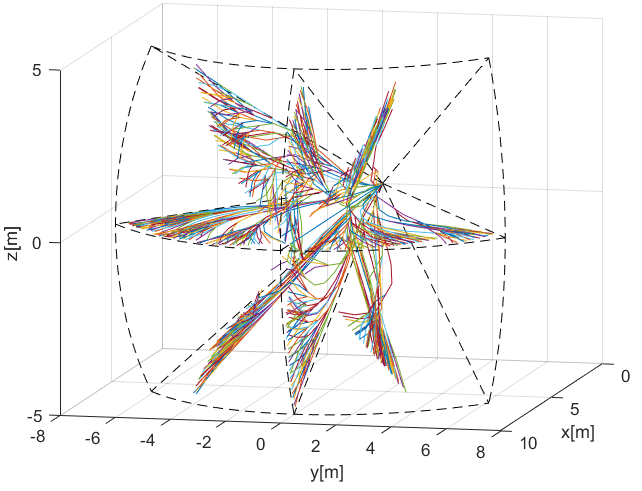
\includegraphics[width=0.9\linewidth]{\FIGDIR/RS005ACASLikeReachSetEstimationMethodFull}
        \caption{Full.}
        \label{fig:acasLikeReachSetFull}
    \end{subfigure}
    \begin{subfigure}{0.48\textwidth}
        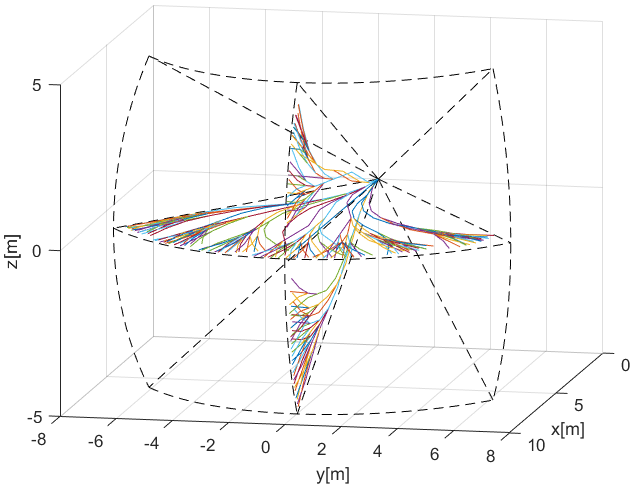
\includegraphics[width=0.9\linewidth]{\FIGDIR/RS006ACASLikeReachSetEstimationMethodHorizontalVertical} 
        \caption{Horizontal-Vertical.}
        \label{fig:acasLikeReachSetHorizontalVertical}
    \end{subfigure}
    \\
    \begin{subfigure}{0.48\textwidth}
        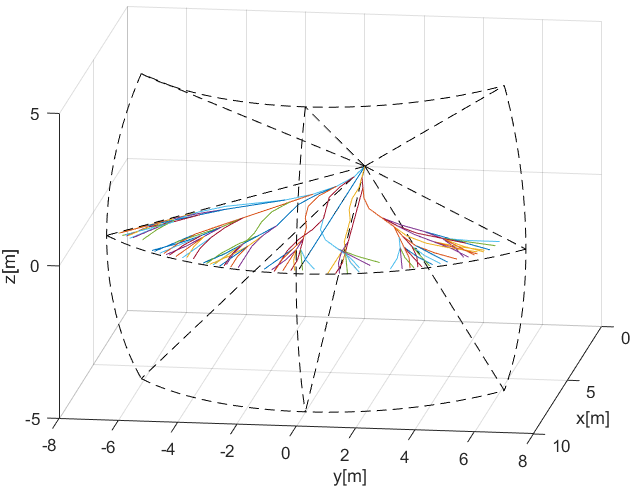
\includegraphics[width=0.9\linewidth]{\FIGDIR/RS008ACASLikeReachSetEstimationMethodHorizontal} 
        \caption{Horizontal.}
        \label{fig:acasLikeReachSetHorizontalOnly}
    \end{subfigure}
    \begin{subfigure}{0.48\textwidth}
        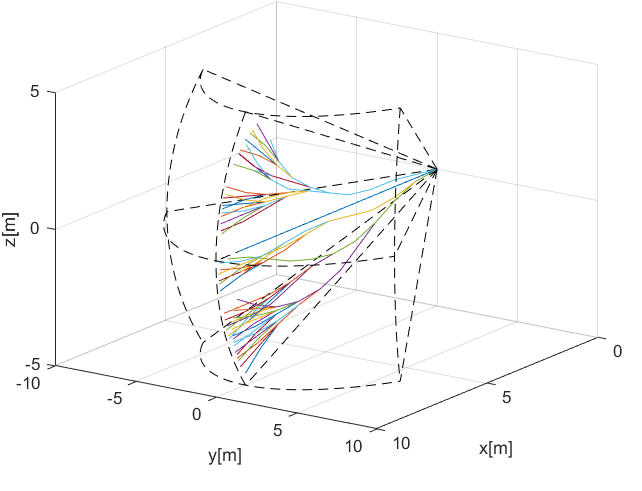
\includegraphics[width=0.9\linewidth]{\FIGDIR/RS009CASLikeReachSetEstimationMethodVertical} 
        \caption{Vertical.}
        \label{fig:acasLikeReachSetVerticalOnly}
    \end{subfigure}
    \caption{ACAS-X imitation \emph{reach set} approximation for various \emph{separation modes}. }
    \label{fig:acasLikeReachSetVariousSeparationMode}
\end{figure}

\paragraph{Pros and Cons:} It can be seen from examples (fig. \ref{fig:acasLikeReachSetVariousSeparationMode}) that \emph{ACAS-like Reach Set Approximation Method} (alg. \ref{alg:ExpansionConstraintFunctionForACASLikeReachSet}) generates full reach set for 2D plane located in 3D space. 

The \emph{Reach Set} contains trajectories with \emph{high coverage ratio} and \emph{high smoothness rating} for selected 2D separation plane. Overall performance compared to full 3D reach sets (sec. \ref{s:chaoticReachSet}, \ref{s:harmonicReachSet} \ref{s:combinedReachSet}) is poor. 

The \emph{node} and \emph{trajectory} count boundary was not implemented. It is common knowledge that \emph{2D} avoidance sets does not require scaling \cite{marston2015acas}. Otherwise trajectory footprint mechanism like in \emph{Harmonic Reach Set Approximation} (alg. \ref{alg:ExpansionConstraintFunctionForHarmonicReachSet}) can be introduced.

This reach set implements \emph{Planar-Separation} as native feature, it can be used for both \emph{navigation} and \emph{avoidance} tasks in \emph{Controlled Airspace}. For \emph{Non-controlled Airspace} there are far more superior \emph{Combined Reach Set} (sec. \ref{s:combinedReachSet}).

	
    \cleardoublepage
\section[Situation Representation in the Avoidance Grid]{Situation Representation \\in the Avoidance Grid}\label{sec:situationAssessment}

\paragraph{Summary:} There is a need to have a safety assessment of the operational space in the form of the Avoidance Grid. Each type of threat coming from different sources (sensors, maps) like obstacles, intruders, and constraints is handled separately. The data fusion procedure provides a unified representation of sourced threats.  

This section gives an overview how different threat is projected into \emph{avoidance grid}:

\begin{enumerate}
	\item\emph{Obstacles} (sec. \ref{s:staticObstacles}) - how static obstacles are represented, how to map data are processed and represented, how the concept of visibility impact certainty of an obstacle in space.
	
	\item\emph{Intruders} (sec. \ref{s:intruders}) - how intruders are projected into avoidance grid, how great is probability to encounter a specific intruder in given space and time.
	
	\item\emph{Constraints} (sec. \ref{s:virtualConstraints}) - how are constraints like geo-fencing or weather represented, how is their impact on space calculated.
	
	\item\emph{Data Fusion} (sec. \ref{s:sensorFusion}) - how is the final threat in cell calculated, how this threat impacts the safety of passing trajectories, how we know which cells in the grid are safe.
\end{enumerate}
    	%Obstacles
    	\cleardoublepage
\section{\secState{R}Static Obstacles and Constraints}\label{s:staticObstacles}
    
\paragraph{Introduction:} The \emph{static obstacles} were used in original concept \cite{gomola2017probabilistic}, the \emph{Avoidance Grid} and \emph{Movement Automaton} were repurposed to enable \emph{finite time deterministic} avoidance. An \emph{Constraint based path search} and \emph{obstacle modeling} is summarized in \cite{hentenryck2009constraint}.

This section is handling basic problems of \emph{static obstacle} detection and its focused on following real-world fixed position threats:
\begin{enumerate}
    \item \emph{Static Obstacles} - detected by LiDAR sensor or fused from \emph{Obstacle Map} information source.
    
    \item \emph{Geo-fencing Areas} - defined by offline/online information source as permanent flight restriction zones. There is usually no physical obstacle. The space is considered as \emph{hard/soft constraint}.
    
    \item \emph{Long-term bad weather Areas} - the \emph{weather} is changing often (hour period), there are \emph{weather events}  which lasts for \emph{hours} or \emph{days}.
\end{enumerate}


\paragraph{Changing Scanning Density of LiDAR:} A LiDAR sensor is scanning in conic section given by $distance Range$, $horizontal Range$, $vertical Range$, where distance range is in interval $[0,maxDistance]$, horizontal offset range is in $[-pi,pi]$, and vertical offset range is in $[\varphi_s, \varphi_e]$.  

Let say that $\text{d} horizontal^\circ, \text{d} vertical^\circ$ is unitary angle offset in which one LiDAR send and return is executed. That means the \emph{LiDAR} ray is sent every $\text{d} horizontal^\circ, \text{d} vertical^\circ$ offset movement. The \emph{LiDAR} ray density is decreasing with \emph{distance offset}. The same amount of \emph{LiDAR} rays passes trough $cell_{i,j,k}$ in Avoidance Grid.

The surface of area given by some distance d, and unitary offsets$\partial horizontal^\circ, \text{d} vertical^\circ$  is changing with $distance$. The minimal triggering area of object surface is not changing. This fact has an impact on count of the hits on object surface. 

The example is given in (fig. \ref{fig:P01CountOfLiDARHits}) where we have two identical objects (red circle) in distances 5 and 10 meters. The closer object consumes 5 LiDAR beam hits and the farther object consumes only 3 LiDAR beam hits. The probability of obstacle encounter is remaining the same for closer and farther object. The \emph{detected obstacle rate} assessment should return the same  detected obstacle collision rate for objects with same scanned surface (with different LiDAR ray hit count).

\begin{figure}[H]
    \centering
    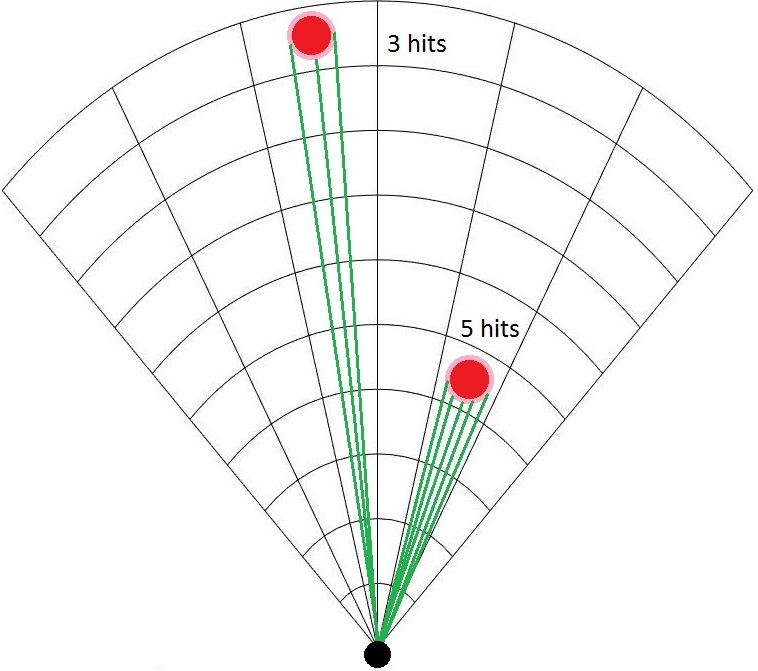
\includegraphics[width=0.7\textwidth]{\FIGDIR/TE051CountOfLiDARHits}
    \caption{Different count of LiDAR hits with different distance from UAS.}
    \label{fig:P01CountOfLiDARHits}
\end{figure}


\paragraph{Map and Detected Obstacles Fusion:} The concept of \emph{offline/online obstacle map} is mandatory in modern obstacle avoidance systems and increases the safety of navigation/avoidance path. The \emph{older} concept was considering only LiDAR reading or \emph{real-time sensor readings} in general \cite{gomola2017probabilistic}. 

\begin{figure}[htbp]
    \centering
    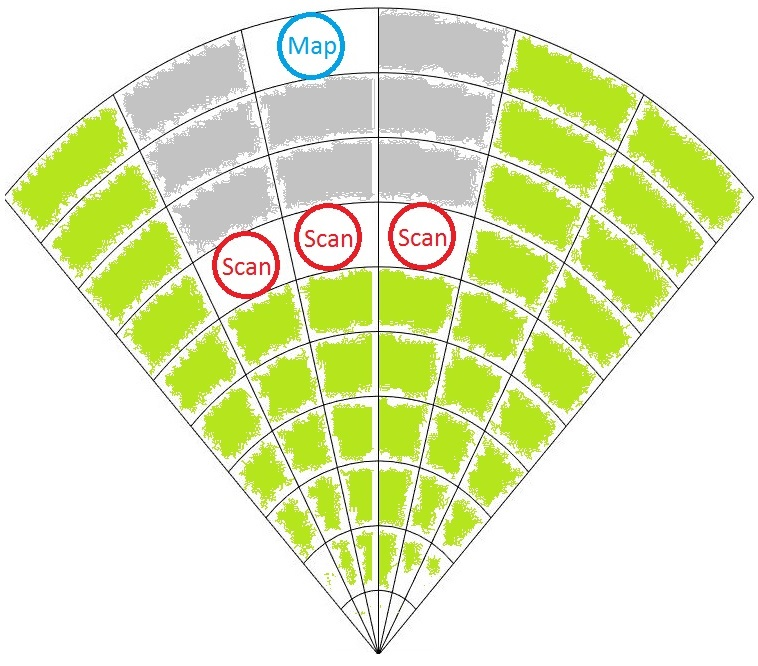
\includegraphics[width=0.7\textwidth]{\FIGDIR/TE053OvershadowedMapobstacle}
    \caption{Overshadowed map obstacle by detected obstacles.}
    \label{fig:P02OvershadowedMapobstacle}
\end{figure}

\newpage\noindent The fusion of real time sensor readings and obstacle map (prior knowledge) is required. Data fusion of these two sources is strongly depending on visibility property, because there are three basic scenarios:

\begin{enumerate}
    \item \emph{Dual detection} - the obstacle is marked on the map and detected by sensory system at some point of the time (older concept works).
    
    \item \emph{Hindered vision} - the detected obstacles are hindering vision to map obstacle therefore map obstacle uncertainty arises (older concept fails). 
    
    \item \emph{False-positive map} - map obstacle occupied space is visible by sensory system, but negative detection is returned. Therefore the map is giving \emph{false-positive} information.
\end{enumerate}

\noindent The second case is given in fig. \ref{fig:P02OvershadowedMapobstacle}, where map obstacle (blue circle) is overshadowed by three scanned obstacles (red circle). The visible space is denoted by green fill, the invisible space is denoted by gray fill. 
    	\subsection{(R) Detected obstacles}\label{s:detectedObstacles}
\paragraph{Idea:} The \emph{visibility} inside avoidance grid and \emph{obstacle} probability are interconnected for most ranging sensors (ex. LiDAR). The goal of this section is to introduce \emph{visibility hindrance} concept which includes space uncertainty assessment and detected obstacle  processing.

\paragraph{Detected Obstacle Rating:} The \emph{detected obstacle rating} defines UAS chances to encounter detected obstacle in avoidance grid $cell_{i,j,k}$. Final \emph{detected obstacle rating} is merged information (eq. \ref{eq:detectedObstacleRatingForCell}). The \emph{sensor field} can contain \emph{multiple} \emph{static obstacle sensors}.

\paragraph{Detected Obstacle Rate for LiDAR:},Lets have only one sensor set as homogeneous two axis rotary LiDAR. For one $cell_{i,j,k}$ there exists set of passing LiDAR beams:

\begin{equation}\label{eq:lidarRaysTroughCell}
    lidar Rays(cell_{i,j,k})=
    \left\{
        \begin{aligned}
        \left[
            \begin{gathered}
                horizontal^\circ\in horizontal Offsets,\\
                vertical^\circ\in vertical Offsets
            \end{gathered}
        \right]\in\R^2:&\\
        horizontal^\circ\in cell_{i,j,k}.horizontal &Range,\\
        vertical^\circ\in cell_{i,j,k}.vertical &Range\\
        \end{aligned}
    \right\}
\end{equation}

\noindent The horizontal and vertical offset of LiDAR ray is homogeneous. Meaning the horizontal/vertical distances between each two neighbouring LiDAR beams are equal.

The set $lidar Rays(cell_{i,j,k}))$ (eq. \ref{eq:lidarRaysTroughCell}) is finite countable and nonempty for any $c_{i,j,k}$, otherwise it will contradict   the definition of avoidance grid (def. \ref{def:AvoidanceGrid}).

The hit function $lidarScan()$ returns a distance of single beam return for beam with dislocation $[horizontal^\circ,$ $vertical^\circ]$ $\in$ $lidar Rays(cell_{i,j,k})$ angle offsets. The set of LiDAR hits (eq. \ref{eq:lidarHitFunction}) in cell $cell_{i,j,k}$ is defined like follow:

\begin{equation}\label{eq:lidarHitFunction}
    lidar Hits(cell_{i,j,k})=\left\{
        \begin{aligned}
        \left[
            \begin{gathered}
                distance=lidar Scan(),\\
                horizontal^\circ\in horizontal Offsets,\\
                vertical^\circ\in vertical Offsets
            \end{gathered}
        \right]\in\R^2:&\\
        distance \in cell_{i,j,k}.distance &Range,\\
        horizontal^\circ\in cell_{i,j,k}.horizontal &Range,\\
        vertical^\circ\in cell_{i,j,k}.vertical &Range\\
        \end{aligned}
    \right\}
\end{equation}

\noindent The \emph{naive} obstacle rate in case of LiDAR sensor defined as ratio between landed hits and possible hits:

\begin{equation}\label{eq:naiveObstacleRate}
    obstacle^{LiDAR}_{cell_{i,j,k}}=\frac{lidar Hits(cell_{i,j,k})}{lidar Rays(cell_{i,j,k})}
\end{equation}

\begin{note}
    The \emph{naive obstacle rate} (eq. \ref{eq:naiveObstacleRate}) ignores that \emph{LiDAR rays} are getting more far apart from each other. The \emph{cell surface} is increasing with cell distance from \emph{UAS}.
\end{note}

\noindent The hindrance (eq. \ref{eq:probabilityOfVisibilityHindrance}) rate is naturally defined as supplement to naive obstacle rate. This definition is sufficient, because its reflecting the \emph{remaining sensing capability} of  LiDAR.

\begin{equation}\label{eq:probabilityOfVisibilityHindrance}
    hindrance^{LiDAR}_{cell_{i,j,k}}=1-\frac{lidar Hits(cell_{i,j,k})}{lidar Rays(cell_{i,j,k})}
\end{equation}

\paragraph{Cell Density Function:}  Let`s start with differential form of cell surface (eq. \ref{eq:finalCellSquare}). The target object have several hits in \emph{Avoidance Grid}. Target $cell_{i,j,k}$ has following properties which are used in surface calculation:
\begin{enumerate}
    \item \textit{Horizontal span} - defines range of horizontal scanner partition.
    \item \textit{Vertical span} - defines range of vertical scanner partition.
\end{enumerate}

\noindent By rewriting (eq. \ref{eq:finalCellSquare}) and using horizontal range parameter and inverted vertical range parameter following surface integral is obtained (eq. \ref{eq:cellSurfaceIntengralDelta}).

\begin{multline}\label{eq:cellSurfaceIntengralDelta}
    Area(cell_{i,j,k}) =\\ \int_{horizontal_{start}^\circ}^{horizontal_{end}^\circ}\int_{vertical_{end}^\circ}^{vertical_{start}^\circ} radius^2 \cos(vertical^\circ) \quad \text{d} vertical^
    \circ\text{d} horizontal^\circ
\end{multline}

\begin{note}
    The \emph{radius} parameter is \emph{average} distance of hits landed in $cell_{i,j,k}$. This helps to reflect real \emph{scanned surface}.
\end{note}

Numerically stable integration exist for boundaries $horizontal^\circ \ in [-\pi,\pi]$, $vertical^\circ \in [-\frac{\pi}{2},\frac{\pi}{2}]$ given as follow:

\begin{multline}\label{eq:intersectionSurfaceForCell}
    Area(radius,horizontal Range, vertical_{start}^\circ, vertical_{end}^\circ) =\dots\\ 
    =\left\{
    \begin{aligned}
        vertical&_{start}^\circ <0, vertical_{end}^\circ \le 0 :\\ 
            &radius^2(\sin |vertical_{start}^\circ| - \sin|vertical_{end}^\circ|)\times horizontal Range)\\
         vertical&_{start}^\circ <0, vertical_{end}^\circ > 0   :\\
            & r^2(\sin |vertical_{start}^\circ| + \sin|vertical_{end}^\circ|)\times horizontal Range)\\
         vertical&_{start}^\circ \ge 0 vertical_{end}^\circ < 0 :\\
            & r^2(\sin vertical_{end}^\circ- \sin vertical_{start}^\circ)\times horizontal Range)
    \end{aligned}
    \right.
\end{multline}

\noindent An intersection surface for cell is defined in (eq. \ref{eq:intersectionSurfaceForCell}). Area covered by LiDAR hits (eq. \ref{eq:lidarHitArea}) is defined as LiDAR hit rate (hits to passing rays ratio) multiplied by \emph{Average} cell intersection surface (eq. \ref{eq:intersectionSurfaceForCell}).

\begin{equation}\label{eq:lidarHitArea}
    lidar Hit Area(cell_{i,j,k}) = \frac{lidar Hits(cell_{i,j,k})}{lidar Rays(cell_{i,j,k})} \times Area\left(\begin{gathered}radius,horizontal Range,\\ vertical_{start}^\circ, vertical_{end}^\circ\end{gathered}\right)
\end{equation}

\noindent There is user defined parameter for \emph{LiDAR treshold area}, which represents minimal considerable surface area for obstacle to be threat. The \emph{detected obstacle rate} considering surface is defined in (eq. \ref{eq:lidarHitFormula}) and it removes bias of naive approach (eq.\ref{eq:naiveObstacleRate}).

\begin{equation}\label{eq:lidarHitFormula}
    obstacle(LiDAR,cell_{i,j,k})=\min\left\{\frac{lidar Hit Area(cell_{i,j,k})}{UAS.lidar Threshold Area},1\right\}
\end{equation}



\paragraph{Visibility Rate for  LiDAR:} For each $cell_{i,j,k}$ and each sensor in sensor field there exist hindrance rate, which defines how much vision is clouded in single cell. Example of hindrance calculation for LiDAR has been given by (eq. \ref{eq:probabilityOfVisibilityHindrance}). Let us consider cell row $cell Row (j_{fix},$ $k_{fix})$ with fixed horizontal index $j_fix$ and vertical index $k_{fix}$ is given as series of cells (eq. \ref{eq:cellrowDefinition}).

\begin{equation}\label{eq:cellrowDefinition}
    cellRow(j_{fix},k_{fix})= \left\{cell_{i,j,k}\in Avoidance Grid :\begin{aligned}&i\in\{1,..,layersCount\},\\&j=j_{fix}, k=k_{fix}\end{aligned}\right\}
\end{equation}

For each $cell_{i,j,k}$ there exists a function which calculates final visibility hindrance rate. Then for ordered cell row:
\begin{equation*}
    cell Row(j_{fix},k_{fix}) = \{cell_{1,j_{fix},k_{fix}},  cell_{2,j_{fix},k_{fix}}, \dots, cell_{layers Count,j_{fix},k_{fix}}\}    
\end{equation*}
and for one selected $cell_{i,j,k}$ the visibility rate is naturally defined as a supplement to hindrance from previous cells. The visibility is defined in (eq. \ref{eq:FinalVisibilityProbability}).

\begin{multline}\label{eq:FinalVisibilityProbability}
    visibility(cell_{i_c,j_c,k_c})=\dots\\ \dots =1 - \sum_{index\in\N^+}^{index < i_c} hindrance(cell_{a,j_c,k_c}: cell_{a,j_c,k_c}\in cell Row(j_{c},k_{c})
\end{multline}

\paragraph{Example:} Let be $cell_{4,j_{fix},k_{fix}}$ is selected for visibility rate assessment, then $cell_{1,j_{fix},k_{fix}}$, $cell_{2,j_{fix},k_{fix}}$, and $cell_{3,j_{fix},k_{fix}}$, are used as a base of cumulative hindrance rate.

\noindent \emph{The cumulative hindrance rate} for any $cell Row(j_{fix},k_{fix})$ is bounded:

\begin{equation}
    0 \le \sum_{cell\in cell Row(j_{fix},k_{fix})} visibility(cell) \le 1
\end{equation}

\begin{note}
    A \emph{cumulative hindrance rate} does not always reach 1 in case of LiDAR sensor, because some rays may pass or hit after leaving \emph{avoidance grid} range.
\end{note}


\begin{figure}[H]
    \centering
    \begin{subfigure}{0.32\textwidth}
        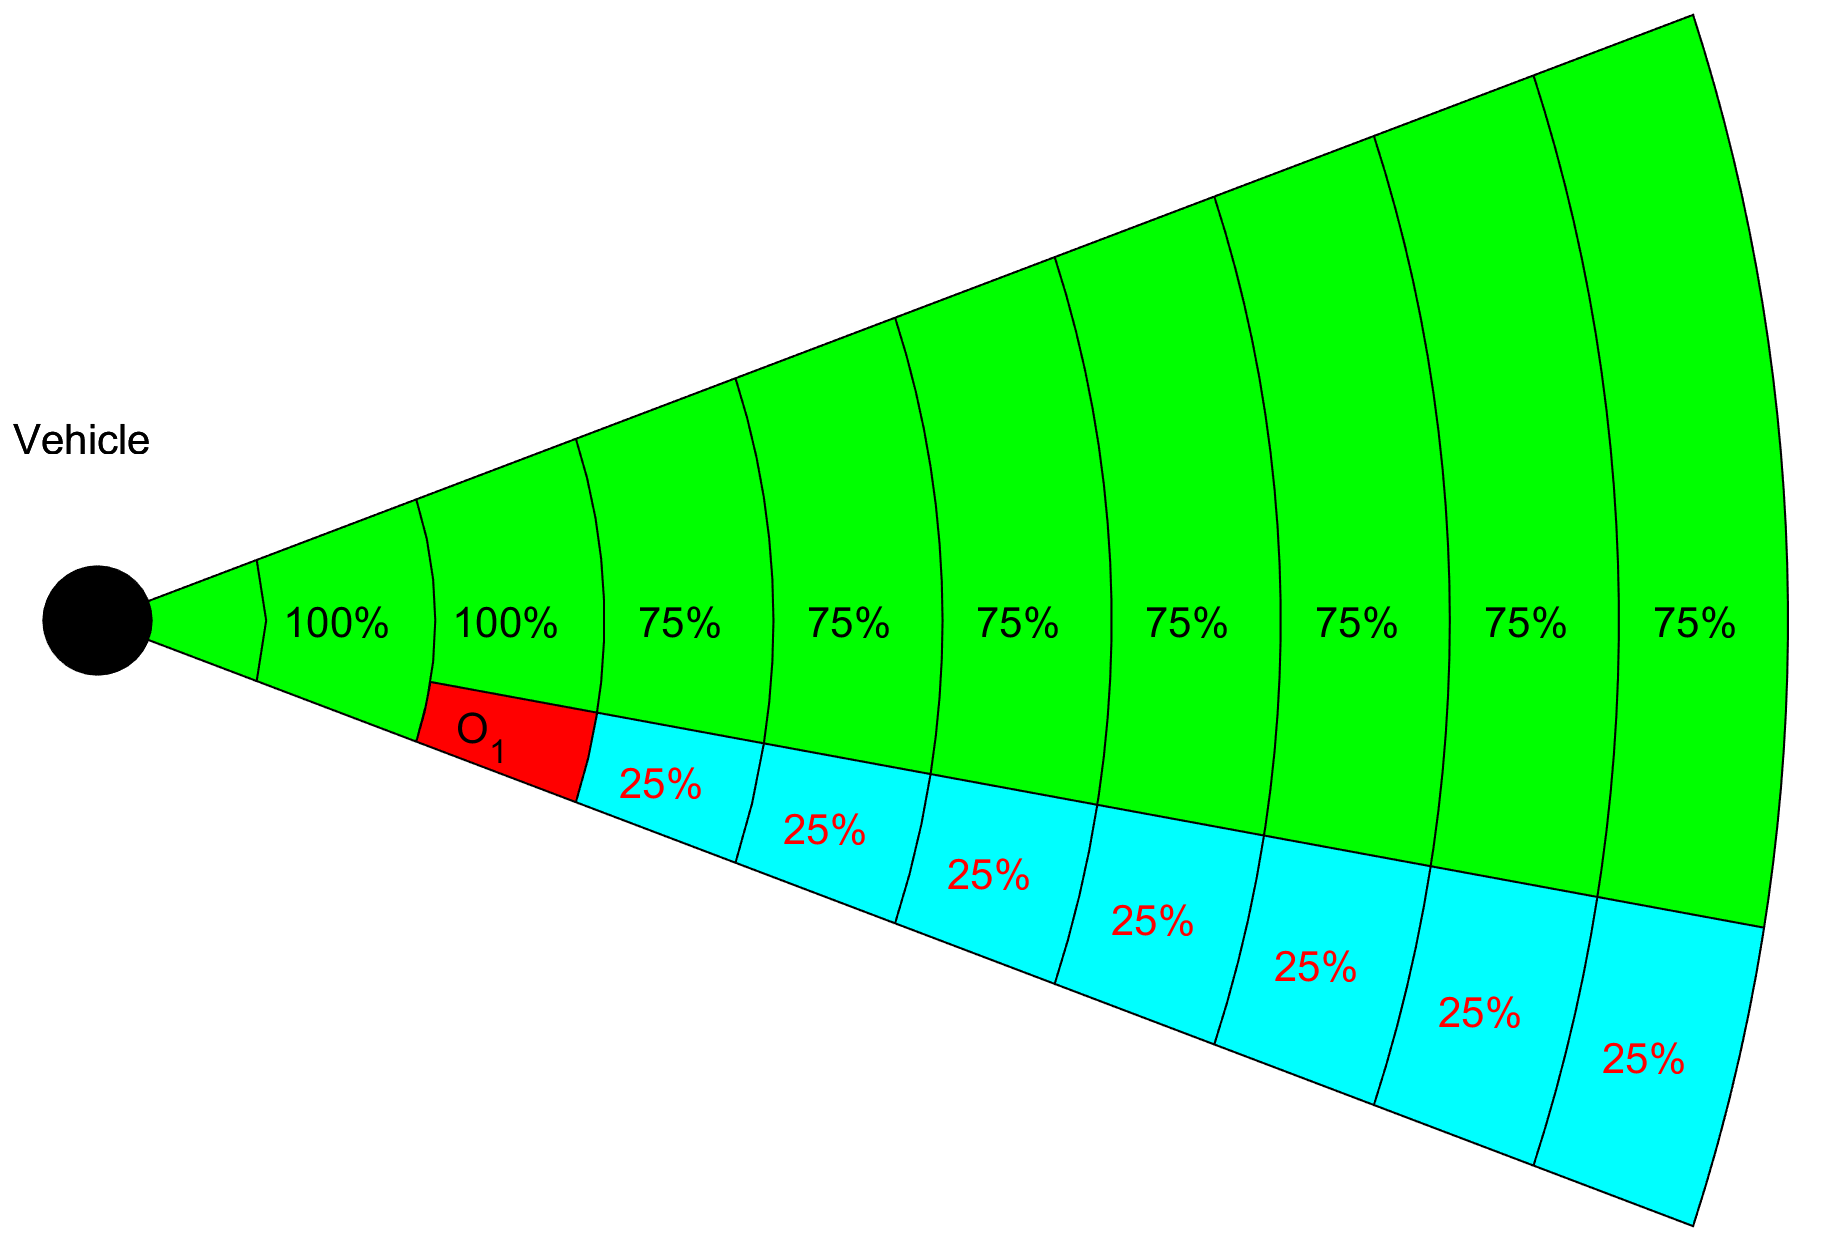
\includegraphics[width=0.9\linewidth]{\FIGDIR/TE006VisibilityFirstObstacle} 
        \caption{1\textsuperscript{st} hindrance.}
        \label{fig:fistObstacleHindrance}
    \end{subfigure}
    \begin{subfigure}{0.32\textwidth}
        \includegraphics[width=0.9\linewidth]{\FIGDIR/TE007VisibilitySecondObstacle} 
        \caption{2\textsuperscript{nd} hindrance.}
        \label{fig:secondObstacleHindrance}
    \end{subfigure}
    \begin{subfigure}{0.32\textwidth}
        \includegraphics[width=0.9\linewidth]{\FIGDIR/TE008VisibilityThirdObstacle} 
        \caption{3\textsuperscript{rd} hindrance.}
        \label{fig:thirdObstacleHindrance}
    \end{subfigure}
    \caption{Obstacle hindrance impact on visibility in \emph{Avoidance Grid Slice}.}
    \label{fig:hindranceImpactOnVisibility}
\end{figure}

For one cell row $cell Row(j_{fix},k_{fix})$, where count of layers is equal to 10, and layers have equal spacing. There is LiDAR sensor

During consequent LiDAR scans $s(t_0)$, $s(t_1)$, $s(t_2)$, and $s(t_3)$ the obstacle sets $\mathscr{O}_1(t_1)=\{o_1\}$, $\mathscr{O}_2(t_2)=\{o_1,o_2\}$, and $\mathscr{O}_3(t_3)=\{o_1,o_2,o_3\}$ are discovered. Assigned hindrance rates are like follow:

\begin{enumerate}
    \item\emph{Time $t_0$} - there is no obstacle nor hindrance, all cells are fully visible.

    \item\emph{Time $t_1$} (fig. \ref{fig:fistObstacleHindrance}) - $\mathscr{O}_1(t_1)=\{o_1\}$ was detected, the hindrance rate  for $cell_{3,j_{fix},k_{fix}})$ is equal to $0.25$. The visibility rate in cells $cells_{4-10,j_{fix},k_{fix}}$ is $0.75$. 
    
    \item\emph{Time $t_2$} (fig. \ref{fig:secondObstacleHindrance}) - $\mathscr{O}_2(t_2)=\{o_1,o_2\}$ was detected, the additional hindrance rate for $cell_{5,j_{fix},k_{fix}}$ is $0.15$. The visibility rate in  $cells_{6-10,j_{fix},k_{fix}}$ is lowered by additional $0.15$ and its set to $0.60$ now.
    
    \item\emph{Time $t_3$} (fig. \ref{fig:thirdObstacleHindrance}) - $\mathscr{O}_3(t_3)=\{o_1,o_2,o_3\}$  was detected the additional hindrance rate for  $cell_{7,j_{fix},k_{fix}}$ is $0.20$. The visibility rate in $cells_{8-10,j_{fix},k_{fix}}$ is lowered by additional $0.20$ and its set to $0.40$  now.
\end{enumerate}
		%\subsection{\secState{R}Map Obstacles}\label{s:mapObstacles}
\paragraph{Map Obstacles:} Use \emph{stored LiDAR readings} from previous mission to build an compact obstacle map \cite{cernamaria2018}. Then use \emph{this map} as a additional information source.

\begin{figure}[H]
    \begin{subfigure}{0.32\textwidth}
        \includegraphics[width=0.9\linewidth]{\FIGDIR/TE009MapObstacleUndetected} 
        \caption{Undetected.}
        \label{fig:undetectedMapObstalce}
    \end{subfigure}
    \begin{subfigure}{0.32\textwidth}
        \includegraphics[width=0.9\linewidth]{\FIGDIR/TE010MapObstacleDetected} 
        \caption{Detected.}
        \label{fig:detectedMapObstacle}
    \end{subfigure}
    \begin{subfigure}{0.32\textwidth}
        \includegraphics[width=0.9\linewidth]{\FIGDIR/TE011MapObstacleHiden}
        \caption{Hindered.}
        \label{fig:hinderedMapObstacle}
    \end{subfigure}
    \caption{Map obstacle states after \emph{Data fusion}.}
    \label{fig:mapObstacleStatesAfterDataFusion}
\end{figure}

\paragraph{Concept:} A \emph{map obstacle} state has very simple logic, there are three possible cases:

\begin{enumerate}
    \item \emph{Undetected} - Map obstacle $O_M$ is charted on map (fig. \ref{fig:undetectedMapObstalce}), but is undetected by any sensor in sensor field, therefore the probability of map obstacle occurrence is equal to $0$.


    \item \emph{Detected} Map obstacle $O_M$ is charted on map and detected by any sensor in sensor field (fig. \ref{fig:detectedMapObstacle}). The map obstacle rate is equal to detected obstacle rate, usually its equal to $1$.

    \item \emph{Hindered} Map obstacle $O_M$ is hindered behind other detected obstacle $O_1$ (fig. \ref{fig:hinderedMapObstacle}). The detected obstacle $O_1$ is in $cell_{i,j,k}$ and is reducing visibility in follow up $cellRow_{i_f>i,j,k}$ by $60$ percent.
\end{enumerate}

\paragraph{Implementation:} The formulation of final map obstacle rate  $map(cell_{i,j,k})$ was outlined in previous examples. These examples are showing the \emph{desired behaviour} and its solved by \emph{data fusion} (sec. \ref{s:sensorFusion}).

First we start with obstacle map definition. The obstacle map  (eq. \ref{eq:obstacleMap}) defines an map obstacle set of information vectors with position in global coordinate frame , orientation bounded to global coordinate reference frame, safety margin and additional parameters.
\begin{equation}\label{eq:obstacleMap}
    obstacle Map= 
    \left\{
    \begin{bmatrix}
        position,\\
        orientation,\\
        safety Margin,\\
        parameters
    \end{bmatrix}
    :
    \begin{aligned}
        & position \in  \R^3(GCF),\\
        & orientation \in \R^3(GCF),\\
        & safety Margin \in \R^+(m),\\
        & parameters \in \{\dots\}
    \end{aligned}
    \right\}
\end{equation}


The \emph{Map Obstacle} concept is taken from my \emph{master student work} \cite{cernamaria2018}, implementing \emph{compact representation} of point-cloud obstacle map. Te example of \emph{cuboid obstacles} with \emph{safe zone} is given in (fig. \ref{fig:exampleExtractedMapObstacles}).
    
\begin{figure}[H]
    \centering
    \includegraphics[width=0.7\textwidth]{\FIGDIR/TE054ExtractedMapObstaclesExample}
    \caption{Example of Extracted Map Obstacle \cite{cernamaria2018}.}
    \label{fig:exampleExtractedMapObstacles}
\end{figure} 

\noindent The space covered by any obstacle  is non-empty by definition. There are following types of map charted obstacles which are implemented in framework:

\begin{enumerate}
    \item\emph{Ball obstacle $parameters=\varnothing$} - simple ball with center at $position$, with offset safety margin.
    
    \item\emph{Line obstacle $parameters=[length]$} - simple line bounded by length $\in]0,\infty[$ with center at $position$ and given orientation with respect to main axis in global coordinate frame, with safety margin $<$ 0.
    
    \item\emph{Plane obstacle $parameters=[length,width]$} - bounded rectangle plane partition defined by length $\in]0,\infty[$, and width $w\in]0,\infty[$ with center at $\vec{p}$ and given orientation $\vec{o}$ with respect to main axis in global coordinate frame, with safety margin.
    
    \item\emph{Cuboid obstacle $parameters=[length,width,depth]$} - bounded cuboid space partition defined by length $\in]0,\infty[$, width $\in]0,\infty[$, and depth $d\in]0,\infty[$ with center at $position$ and rotated in orientation with respect to main axis in global coordinate frame, with safety margin.
\end{enumerate}

\noindent The \emph{map obstacles} are stored in clustered database. The \emph{selection criterion} is given in (eq. \ref{eq:mapObstacleSelectionCriterion}).

\begin{equation}\label{eq:mapObstacleSelectionCriterion}
    avoidance Grid.radius \ge distance(UAS.position,map Obstacle) - total Margin
\end{equation}

\noindent The \emph{total margin} is combination of \emph{safety margin} and \emph{body margin} (in case of line, plane, cuboid obstacle). The \emph{selection} was implemented as standard cluster select, selecting 26  surrounding clusters around UAS + own UAS cluster.

\noindent The \emph{compact obstacle representation} is transformed into \emph homogeneous point-cloud representations:

\begin{itemize}
    \item[1.]\emph{Body Point-cloud} - representing obstacle body approximation by geometrical shape (eq. \ref{eq:mapBodyPointCloud}). This point cloud is considered as hard constraints.
    
    \begin{equation}\label{eq:mapBodyPointCloud}
        body Point Cloud  =\{point\in\R^3(GCF): point \in map Obstacle Body\}
    \end{equation}
    
    \item[2.]\emph{Safety Margin Point Cloud} - representing safety coating around mapped obstacle body approximation (eq. \ref{eq:mapMarginPointCloud}). This point cloud is considered as soft constraint.
    \begin{equation}\label{eq:mapMarginPointCloud}
        margin Point Cloud = \{point\in\R^3(GCF): point \in map Safety Margin\}
    \end{equation}
\end{itemize}

\begin{note}
    The \emph{safety margin point cloud} is hollow in relationship to an \emph{body point cloud}, therefore:
    \begin{equation*}
        body Point Cloud \cap margin Point Cloud  = \varnothing
    \end{equation*}
\end{note}

\noindent The \emph{map obstacle} discretization to point cloud leads to problem how to calculate \emph{impact rate}. The \emph{theoretical impact rate} for \emph{obstacle} is given as:
\begin{equation*}
    impact Rate = \frac{volume(map Obstacle\cap cell_{i,j,k})}{volume(cell_{i,j,k})}\in [0,1]
\end{equation*}

\noindent The \emph{map obstacle related point clouds} (eq. \ref{eq:mapBodyPointCloud}, \ref{eq:mapMarginPointCloud}) are homogeneous \cite{cernamaria2018}. That means \emph{each point} in point clouds covers similar portion of object volume. There is \emph{threshold volume} (eq. \ref{eq:tresholdVolumeDefinition}) which represents minimal object volume to be considered as an \emph{obstacle}.

\begin{equation}\label{eq:tresholdVolumeDefinition}
    0< threshold Volume \le \frac{volume(point Cloud)}{|point Cloud|}
\end{equation}

\noindent The \emph{impact rate} of one point  when intersecting a $cell_{i,j,k}$ is given as count of \emph{threshold obstacle bodies} in \emph{point cloud covered mass} multiplied by inverted point count (eq. \ref{eq:pointImpactRateMap}).

\begin{equation}\label{eq:pointImpactRateMap}
    point. rate = \frac{point Cloud Volume}{threshold Volume}\times\frac{1}{|point Cloud|}
\end{equation}

The \emph{intersection set} between \emph{point cloud} and $cell_{i,j,k}$ is defined in (eq. \ref{eq:pointImpactRateMap}). The \emph{cell} intersection with points is defined in (eq. \ref{eq:boundedSpaceCell}).

\begin{multline}\label{eq:pointcloudIntersectionMap}
    intersection(map,cell_{i,j,k}) =\dots\\\dots \{points \in \R^3: (point\to Avoidance Grid Frame) \in cell_{i,j,k}\}
\end{multline}

\newpage \noindent The \emph{map obstacle rating} for $cell_{i,j,k}$ and obstacle for our \emph{information source} is defined in (eq. \ref{eq:mapcellratingourMap}).

\begin{equation}\label{eq:mapcellratingourMap}
    map(cell_{i,j,k},obstacle) =\max\left\{ \sum_{\forall point\in intersection(map,cell_{i,j,k})}  point.rate , 1\right\}
\end{equation}

\noindent The \emph{map obstacle rating} for $cell_{i,j,k}$ and \emph{our information source} is given as maximum of all possible cumulative ratings form each obstacle in \emph{active map obstacles} set (eq. \ref{eq:cumulativeMapCellRatingMap}).

\begin{equation}\label{eq:cumulativeMapCellRatingMap}
    map(cell_{i,j,k} = \max \left\{map(cell_{i,j,k},obstacle):\forall obstacle \in Active Map Obstacles\right\}
\end{equation}

\begin{note}
    The \emph{body point clouds} (eq. \ref{eq:mapBodyPointCloud}) never intersects, because they are created for inclusive obstacles. The \emph{safety margin point clouds} (eq. \ref{eq:mapMarginPointCloud}) can intersects, because they represents protection zones around physical obstacles. Therefore the \emph{maximum obstacle rating} (eq. \ref{eq:cumulativeMapCellRatingMap}) needs to be selected.
\end{note}

	    %Intruders
    	\subsection{Intruders}\label{s:intruders}
\paragraph{Intruder behavior:} \emph{Adversarial behavior} of moving obstacle is trying to destroy avoiding our UAS.  The \emph{Intruder} UAS \cite{fiorini1998motion} is not trying to hurt our \emph{UAS} actively. The \emph{Adversarial behaviour} is neglected in this work. The non-cooperative avoidance is assumed, it can be relaxed to \emph{cooperative avoidance} in \emph{UTM controlled airspace}.

\paragraph{Intruder information:} The \emph{observable intruder information set} for any kind of intruder, obtained through the sensor/C2 line, is following:
\begin{enumerate}
    \item\emph{Position} - position of an intruder in the \emph{local} or \emph{global} coordinate frame, which can be transformed into \emph{avoidance grid coordinate frame}.
    
    \item\emph{Heading and Velocity} - intruder heading and linear velocity in avoidance grid coordinate frame.
    
    \item\emph{Horizontal/Vertical Maneuver Uncertainty Spreads} - how much can an \emph{intruder} deviate from the \emph{original linear path} in a \emph{horizontal/vertical} plane in \emph{Global coordinate Frame}.
\end{enumerate}

 

\begin{figure}[H]
    \centering
    \includegraphics[width=0.7\textwidth]{\FIGDIR/TE052AdversaryProbabilitySpread}
    \caption{Intruder UAS intersection rate along the expected trajectory.}
    \label{fig:intruderProbabiltySpreadTheoretical}
\end{figure}   

\paragraph{Example of Intruder Intersection:} Let us neglect the \emph{time-impact} aspect on the \emph{intersection}.  The \emph{intruder} (black "I" circle) is intersecting one \emph{avoidance grid horizontal slice} (fig. \ref{fig:intruderProbabiltySpreadTheoretical}).  The intruder is moving along linear path approximation based on velocity (middle green line). The \emph{Horizontal Maneuver Uncertainty spread} is in \emph{green line boundary area} \emph{intruder intersection rating} is denoted as green-orange-red cell fill reflecting intersection severity:  red is a high rate of the intersection, orange is the medium rate of the intersection and green is a low rate of the intersection.
    


\paragraph{Moving Threats:} The \emph{UAS} can encounter following threats during the \emph{mission execution}:
\begin{enumerate}
    \item \emph{Non-cooperative Intruders} - the intruders who does not implement any approach to ensure mutual avoidance efficiency.
    
    \item \emph{Cooperative Intruders} - the intruders whom actively communicate or follow common agreed behavior pattern (ex. Rules of the Air).
    
    \item \emph{Moving Constraints} - the constrained portion of \emph{free} space which is shifting its boundary over time (ex. Short term bad weather).
\end{enumerate}
    
\begin{note}
    Our approach considers only \emph{UAS} intruders because \emph{Data Fusion} considers data received through \emph{ADS-B} messages. The \emph{Intruders} extracted from \emph{LiDAR} scan were not considered (ex. birds). The proposed \emph{intruder intersection models} are reusable for other \emph{intruder sources}.
\end{note}

\paragraph{Approach Overview:} The \emph{Avoidance Grid} (def. \ref{def:AvoidanceGrid}) is adapted to the \emph{LiDAR} sensor. The \emph{Euclidean grid intersections} are fairly simple. The \emph{polar coordinates grid} is not. The need to keep \emph{polar coordinates grid} is prevalent, because of fast \emph{LiDAR} reading assessment.  There are following commonly known methods to address this issue:

\begin{enumerate}
    \item\emph{Point-cloud Intersections} - the \emph{threat impact area} is discredited into a sufficiently thick point cloud. This point-cloud have \emph{point impact rate} and \emph{intersection time} assigned to each point. The \emph{point-cloud} is projected to \emph{Avoidance Grid}. If the \emph{impact point} hits $cell_{i,j,k}$ the cell`s impact rate is increased by the amount of \emph{point impact rate}. The final \emph{threat impact rate} in $cell_{i,j,k}$ is given when \emph{all} points from point cloud are consumed. Close point problem \cite{shamos1975closest} was solved by the application of method  \cite{bentley1980optimal}.
    
    \item\emph{Polygon Intersections} - the \emph{threat impact area} is modeled as a polygon, each $cell_{i,j,k}$ in \emph{Avoidance Grid} is considered as a \emph{polygon}. There is a possibility to calculate cell space geometrical inclusive intersection. The \emph{impact rate} is then given as rate between \emph{intersection volume} and $cell_{i,j,k}$ volume. The algorithm used for intersection selected based on:\citep{bentley1979algorithms} the selected algorithm  \emph{Shamos-Hoey} \cite{shamos1976geometric}.
\end{enumerate}

\begin{note}
    The \emph{Intruder Intersection} models are based on \emph{analytical geometry} for \emph{cones and ellipsoids} taken from \cite{sommerville2016analytical}.
\end{note}

    	\subsection{(R) Intruder Behaviour Prediction}\label{s:intruderBehaviourPrediction}
\paragraph{Idea:} \emph{Intruder Intersection Models} is about space-time intersection of \emph{intruder body} with \emph{avoidance Grid} and \emph{Reach Set}:
\begin{enumerate}
    \item The \emph{UAS} reach set defines \emph{time boundaries} to \emph{enter/leave} cell in avoidance grid.
    \item The \emph{Intruder} behavioral pattern defines \emph{rate} of \emph{space intersection} with cell bounded space in avoidance grid.
\end{enumerate}

The multiplication of \emph{space intersection rate} and \emph{time intersection rate} will give us \emph{intruder intersection} rate for our \emph{UAS} and intruder.


\paragraph{Intruder Dynamic Model:} The  definition of avoidance grid enforces the  most of these methods to be numeric. Let us introduce intruder dynamic model:

\begin{equation}\label{eq:intruderBasicLinearModel}
    \begin{aligned}
        \partial position /\partial time = velocity 
    \end{aligned}
    \quad | \quad
    \begin{aligned}
        position_x(t) = position_x(0) + velocity_x \times t\\
        position_y(t) = position_y(0) + velocity_y \times t\\
        position_z(t) = position_z(0) + velocity_z \times t
    \end{aligned}
\end{equation}

\noindent Position vector in euclidean coordinates $[x,y,z]$   is transformed into \emph{Avoidance Grid} coordinate frame. Velocity vector for $[x,y,z]$  is \emph{estimated and not changing}. The time  is in interval $[entry,leave]$, where $entry$ is intruder entry time into avoidance grid and $leave$ is intruder leave time from avoidance grid. 

\begin{note}
    If \emph{intruder} is considered, time of entry is marked as $intruder_{entry,k}$ where k is intruder identification, time of leave is marked as $intruder_{leave,k}$ where k is intruder identification. 
\end{note}

\paragraph{Cell Entry and Leave Times} $UAS_{entry}(cell_{i,j,k})$ and $UAS_{leave}(cell_{i,j,k})$ are depending on intersecting  \emph{Trajectories} and \emph{bounded cell space} (eq. \ref{eq:boundedSpaceCell}). There is \emph{Trajectory Intersection} function from (def. \ref{def:ContainedReducedReachSet}) which evaluates \emph{Trajectory segment} entry and leave time. 

The UAS \emph{Cell Entry} time is given as minimum of all \emph{passing trajectory segments} entry times (eq. \ref{eq:cellEntryTime}), if there is no \emph{passing trajectories} the UAS \emph{entry time} is set to 0.

\begin{equation}\label{eq:cellEntryTime}
    UAS_{entry}(cell_{i,j,k}) =  \min 
    \left\{\begin{aligned}
    0,en&try(Trajectory,cell_{i,j,k}):\\ &Trajectory\in Passing Trajectories
    \end{aligned}\right\}
\end{equation}

The UAS \emph{Cell Leave} time is given as maximum of all \emph{passing trajectory segments} entry times (eq. \ref{eq:cellLeaveTime}), if there is no \emph{passing trajectories} the UAS \emph{leave time} is set to 0.

\begin{equation}\label{eq:cellLeaveTime}
    UAS_{leave}(cell_{i,j,k}) =  \max 
    \left\{\begin{aligned}
    0,lea&ve(Trajectory,cell_{i,j,k}):\\ &Trajectory\in Passing Trajectories
    \end{aligned}\right\}
\end{equation}

\paragraph{Time Intersection Rate:} The key idea is to calculate how long the \emph{UAS} and \emph{Intruder} spends together in same space portion ($cell_{i,j,k}$). 
The \emph{Intruder} can spent some time in $cell_{i,j,k}$ bounded by interval of \emph{intruder} entry/leave time. 

The \emph{UAS} can spent some time, depending on \emph{selected trajectory} from \emph{Reach Set}. The time spent by UAS is bounded by entry (eq. \ref{eq:cellEntryTime}) and leave (eq. \ref{eq:cellLeaveTime}). 

The intersection duration of these two intervals creates \emph{time intersection rate} numerator, the \emph{maximal duration} of \emph{UAS} stay gives us \emph{denominator}. The \emph{time intersection rate} is formally defined in (eq. \ref{eq:timeIntersectionRate}). 

\begin{equation}\label{eq:timeIntersectionRate}
    time\left(\begin{gathered}UAS,\\Intruder,\\cell_{i,j,k}=\circ\end{gathered}\right)=  
    \frac{
        \left|
        \begin{gathered}
            \ [intruder_{entry}(\circ),intruder_{leave}(\circ)] \\
            \cap\\
            [UAS_{entry}(\circ),UAS_{leave}(\circ)]
        \end{gathered}\right|
        }
        {
        \left|\left[UAS_{entry}(\circ),UAS_{leave}(cell_{\circ})\right]\right|
        }
\end{equation}


\paragraph{Intruder Intersection Rate:} The \emph{Intruder Intersection Rate} (eq. \ref{eq:intruderIntersectionProbability}) is calculated as \emph{multiplication} of \emph{space intersection rate} (defined later) and \emph{time intersection rate} (eq. \ref{eq:timeIntersectionRate}).

\begin{equation}\label{eq:intruderIntersectionProbability}
    intruder\left(\begin{gathered}UAS,\\Intruder,\\cell_{i,j,k}\end{gathered}\right) = time \left(\begin{gathered}UAS,\\Intruder,\\cell_{i,j,k}\end{gathered}\right) \times space\left(\begin{gathered}UAS,\\Intruder,\\cell_{i,j,k}\end{gathered}\right)
\end{equation}

\begin{note}
    If there is no information to derive \emph{Intruder} entry/leave time for cells the \emph{time intersection rate} is considered 1.
\end{note}

The \emph{Intruder cell reach} time (eq. \ref{eq:intruderIntersectionTimeonPoint}) is bounded to discrete point in intersection model \cite{shamos1975closest,bentley1980optimal}. The intruder \emph{entry/leave time} is calculated similar to \emph{UAS cell entry (eq. \ref{eq:cellEntryTime})/leave (eq. \ref{eq:cellLeaveTime}) time}.

\begin{equation}\label{eq:intruderIntersectionTimeonPoint}
    point Reach Time(Intruder,point) = \frac{distance(Intruder.initial Position, point)}{|Intruder.velocity}
\end{equation}


\paragraph{Space Intersection Rate:} The \emph{Space Intersection Rate} reflects probability of \emph{Intruder} intersection with portion of space bounded by $cell_{i,j,k}$, to be precise with intruder trajectory or vehicle body shifted along the trajectory. The principles for \emph{space intersection rate} calculation are following:




\begin{enumerate}
    \item \textit{Line trajectory} - \emph{intruder} trajectory is given by linear approximation (eq. \ref{eq:intruderBasicLinearModel}), depending on \emph{intruder size} the intersection with avoidance grid can be:
    
    \begin{enumerate}[a.]
        \item \emph{Simple line} - intersection is going along the trajectory line line defined by intruder model (eq.\ref{eq:intruderBasicLinearModel}).
    
        \item \emph{Volume line} - intersection is going along the trajectory line defined by intruder model (eq. \ref{eq:intruderBasicLinearModel}) and intruder`s \emph{body radius} is considered in intersection.
    \end{enumerate}
    
    \item \emph{Elliptic cone} - initial position is considered as the top of a cone, the main cone axis is defined by intruder linear trajectory (eq. \ref{eq:intruderBasicLinearModel}) $time \in [0,\infty]$. The cone width is set by horizontal and vertical spread.
\end{enumerate}

		%Constraints    	
    	\subsection{Constraints}\label{s:virtualConstraints}
\paragraph{Static Constraints:} The \emph{constraints} (ex. weather, airspace) usually covers a large portion of the \emph{operation airspace}. 

Converting constraints into valued \emph{point-cloud} is not feasible, due to the \emph{huge amount of created points} and low \emph{intersection rate}. The \emph{polygon intersection} or \emph{circular boundary of a 2D polygon} is a simple and effective solution \cite{ritter1990efficient,welzl1991smallest}. 

The key idea is to create \emph{constraint barrels} around dangerous areas. Each \emph{constraint barrel} is defined by a circle on the \emph{horizontal plane} and the \emph{vertical limit range}.

\paragraph{Representation:} The \emph{minimal representation} is based on (sec. \ref{sec:WellClear}, \ref{sec:WeatherImpact}) and geo-fencing principle. The \emph{horizontal-vertical separation} is ensured by \emph{projecting boundary} as 2D polygon oh horizontal plane and \emph{vertical boundary} (barrel height) as \emph{altitude limit}. 

The \emph{static constraint} (eq. \ref{eq:staticConstraint}) is defined as a structure vector including:
\begin{enumerate}
    \item \emph{Position} - the center position in the global coordinates\emph{2D horizontal plane}.
    
    \item \emph{Boundary} - the ordered set of boundary points forming edges in the global coordinates\emph{2D horizontal plane}.
    
    \item \emph{Altitude Range} - the \emph{barometric altitude} range $[altitude_{start},$ $altitude_{end}]$.
    
    \item \emph{Safety Margin} - the \emph{protection zone} (soft constraint) around constraint body (hard constraints) in meters.
\end{enumerate}

\begin{equation}\label{eq:staticConstraint}
    constraint = \{position,boundary, altitude_{start},altitude_{end}, safety Margin\}
\end{equation}

\paragraph{Active constrain selection:} The \emph{active constraints} are constraints which are impacting \emph{UAS active avoidance range}. 

The \emph{active constraints set} (eq. \ref{eq:activeConstraintSet}) is defined as a set of \emph{constraints} from all \emph{reliable Information Sources} where the \emph{distance} between UAS and constraint body (including safety margin) is lesser than the avoidance grid range. The \emph{horizontal altitude range} of avoidance grid must also intersect with \emph{constraint altitude range}.

\begin{multline}\label{eq:activeConstraintSet}
    Active Constraints = \dots\\\dots =
    \left\{\begin{aligned}constraint& \in Information Source:\\ 
    &distance(constraint,UAS) \le Avoidance Grid. distance,\\
    &constraint.altitude Range \cap UAS.altitude Range \neq \varnothing 
    \end{aligned}\right\}
\end{multline}

\paragraph{Cell Intersection:} The \emph{importance of constraints} is on their impact on \emph{avoidance grid} $cells$. The \emph{most of the constraints} (weather, ATC) are represented as 2D convex polygons. Even the \emph{irregularly shaped constraints} are usually split into smaller convex 2D polygons.

The idea is to represent convex polygon boundary as a sufficiently large circle to cover polygon. The Welzl algorithm to find \emph{minimal polygon cover circle} \cite{welzl1991smallest} is used.

First the \emph{set of contraint edges} (eq. \ref{eq:constraintEdgeSet}) is a enclosed set of 2D edges between neighboring points defined as follow:

\begin{equation}\label{eq:constraintEdgeSet}
    edges(constraint) =
    \left\{
    \begin{bmatrix}
        point_{i},point_{j}
    \end{bmatrix}:
    \begin{aligned}
    &point\in boundary,\\
    &i \in \{1,\dots,|boundary|\},\\
    &j \in \{2,\dots, |boundary|,1\}\\
    \end{aligned}
    \right\}
\end{equation}

\noindent The \emph{constraint circle boundary} with calculated center on the  2D horizontal plane and radius (representing body margin) is defined in (eq. \ref{eq:constraintCircleBoundary}).

\begin{equation}\label{eq:constraintCircleBoundary}
    circle(constraint)=
    \left[
        \begin{aligned}
            & center = \frac{\sum boundary.point}{|boundary.point|} + correction\\
            & radius = smallest Circle(edges(constraints)) 
        \end{aligned}
    \right]
\end{equation}

\noindent The $(cell_{i,j,k}$ and \emph{constraint} intersection (eq. \ref{eq:contraintToCellIntersection}) is classification function. The \emph{classification} is necessary, because one \emph{constraint} induce: 
\begin{enumerate}
    \item \emph{Body Constraint} (hard constraint) - the distance between $cell_{i,j,k}$ closest border and \emph{circular boundary} center is in interval $[0,radius]$.
    
    \item \emph{Protection Zone Constraint} (soft constraint) - the distance between $cell_{i,j,k}$ closest border and \emph{circular boundary} center is in interval $]radius,radius+safety Margin]$.
\end{enumerate}


\begin{multline}\label{eq:contraintToCellIntersection}
    intersection,constraint)=\dots\\\dots = 
    \begin{cases}
        hard &:\left[
            \begin{aligned}
                &distance(cell_{i,j,k},circle(constraint)) \le\dots\\ 
                &\quad\dots\le circle(constraint).radius,\\
                & constraint.altitude Range \cap cell_{i,j,k}.altitude Range \neq \varnothing,
            \end{aligned}\right]\\
             &\\
        soft &:\left[
            \begin{aligned}
                &distance(cell_{i,j,k},circle(constraint)) >\dots\\ 
                &\quad\dots > circle(constraint).radius,\\
                &distance(cell_{i,j,k},circle(constraint)) \le\dots\\ 
                &\quad\dots\le circle(constraint).radius + safety Margin,\\
                & constraint.altitude Range \cap cell_{i,j,k}.altitude Range \neq \varnothing,
            \end{aligned}\right]\\
             &\\
        none &:otherwise
    \end{cases}
\end{multline}

\noindent The \emph{intersection impact} of constraint is handled separately for \emph{soft} and  \emph{hard} constraints. The \emph{avoidance} of hard constraints is \emph{mandatory}, the \emph{avoidance} of soft constraints is \emph{voluntary}.

The constraints which have a \emph{soft intersection with the cell} are added to cells impacting constraints set: 
\begin{equation}\label{eq:softConstraintsCellIntersections}
    cell_{i,j,k}. soft Constraints = 
    \left\{
        \begin{aligned}
            &constraint \in Active Constraints:\\ 
            &\quad intersection(cell_{i,j,k},constraint) = soft
        \end{aligned}
    \right\}
\end{equation}

\noindent The constraints which have a \emph{hard intersection with the cell} are added to cells impacting constraints set:

\begin{equation}\label{eq:hardConstraintsCellIntersections}
    cell_{i,j,k}. hard Constraints = 
    \left\{
        \begin{aligned}
            &constraint \in Active Constraints:\\ 
            &\quad intersection(cell_{i,j,k},constraint) = hard
        \end{aligned}
    \right\}
\end{equation}

\begin{note}
    The final \emph{constraint rate value} (eq. \ref{eq:constraintRatingForCell}) is determined based on \emph{mission control run} feed to \emph{avoidance grid} (fig. \ref{fig:missionControlRunActivityDiagram}) defined in  7\textsuperscript{th} to the 10\textsuperscript{th} step.
\end{note}
    

    	\subsection{(W) Moving Constraints}\label{s:MovingVirtualConstraints}
\paragraph{Idea:} The basic ideas is the same as in case \emph{static constraints} (sec. \ref{s:virtualConstraints}). There is horizontal constraint and altitude constraint outlining the constrained space. The only additional concept is moving of \emph{constraint} on horizontal plane in global coordinate system. 

The constraint intersection  with \emph{avoidance grid} is done in \emph{fixed decision Time}, for cell in \emph{fixed cell leave time} (eq. \ref{eq:cellLeaveTime}), which means concept from static obstacles can be fully reused.

\paragraph{Definition:} The \emph{moving constraint definition} (eq. \ref{eq:movingConstraintDefinition}) covers minimal data scope for  moving constraint, assuming linear constraint movement. 

The original definition (eq. \ref{eq:staticConstraint}) is enhanced with additional parameters to support constraint moving:

\begin{enumerate}
    \item \emph{Velocity} - velocity vector on 2D horizontal plane.
    
    \item \emph{Detection time} - the time when \emph{constraint} was created/detected, this is the time when \emph center and boundary points position were valid.
\end{enumerate}

\begin{multline}\label{eq:movingConstraintDefinition}
    constraint = \{position,boundary,\dots\\\dots, velocity, detection Time, \dots \\\dots altitude_{start},altitude_{end}, safety Margin\}
\end{multline}

\paragraph{Cell Intersection:} The \emph{intersection algorithm} follows (eq. \ref{eq:contraintToCellIntersection}), only shift of the \emph{center and boundary points} is required. 

First let us introduce $\Delta time$ (eq. \ref{eq:deltatimeMovingconst}), which represents difference between the constraint detection time and expected cell leave time (eq. \ref{eq:cellLeaveTime}).

\begin{equation}\label{eq:deltatimeMovingconst}
    \Delta time = UAS_{leave}(cell_{i,j,k}) - detection Time
\end{equation}

\noindent The constraint boundary is shifted to:

\begin{multline}
    shifted Boundary(constraint) = \{new Point = point + velocity \times \Delta time:\dots\\\dots \forall point \in constraint.boundary \}
\end{multline}

\noindent The constraint center is shifted to:

\begin{equation}
    shifted Center(constraint) = constraint.center + velocity
\end{equation}

\begin{note}
    The $\Delta time$ is calculated separately for each $cell_{i,j,k}$, because \emph{UAS} is also  moving and reaching cells in different times. The \emph{cell leave time} can be calculated in advance after reach set approximation.
\end{note}

\paragraph{Alternative Intersection Implementation:} The alternative used for intersection selected based on polygon intersection algorithms review \citep{bentley1979algorithms}, the selected algorithm  is \emph{Shamos-Hoey} \cite{shamos1976geometric}.

The implementation was tested on \emph{Storm scenario} (sec. \ref{s:testStorm}) and it yelds same results.

    	%Data Fusion
    	\subsection{Data fusion}\label{s:sensorFusion}

\paragraph{Summary:} There is a need for the final threat assessment in the Avoidance Grid. The data fusion provides mechanisms to represent, process, and assess threat in the cell including the safety of trajectories in the RSA. The output of the data fusion procedure is used further in Avoidance run (sec. \ref{s:aviudabceGridRun}).


\paragraph{Introduction:} The data fusion interfaces \emph{Sensor Field} and \emph{Information Sources} from \emph{cell/trajectory properties}. The \emph{Data Fusion Function} is outlined in (\ref{eq:DataFusionFunction}). 

First, there will be an outline of \emph{Partial Rating} commutation. Then these ratings will be discredited into Boolean values as properties of \emph{Avoidance Grid/Trajectory}. Then these Boolean values will be used for further classification of  space into \emph{Free(t), Occupied(t), Restricted(t)} and \emph{Uncertain(t)}.

All mentioned ratings are the result of \emph{Filtered Sensor Readings} from \emph{Sensor Field} and \emph{Information Sources} with prior processing. This section will focus on \emph{final fuzzy value calculation} and \emph{discretization}. 
\begin{note}
    All rating values are in the \emph{range:} $[0,1]$, and they were introduced in previous sections.
\end{note}


\paragraph{Visibility:} The \emph{sensor reading} of \emph{sensor} if \emph{Sensor field} returns a value of \emph{visibility} for cell space in time of decision $t_i$.

The \emph{visibility} for the cell is given in (eq. \ref{eq:visibilityForCell}) as minimal visibility calculated from all capable sensors in \emph{Sensor Field}.

\begin{equation}\label{eq:visibilityForCell}
    visibility(cell_{i,j,k}) = \min \left\{\begin{aligned}visibility(cell_{i,j,k},&sensor_i):\\&\forall sensor_i \in Sensor Field\end{aligned}\right\}
\end{equation}

\noindent The example of \emph{visibility} calculation for \emph{LiDAR} sensor is given in (fig. \ref{fig:mapObstacleStatesAfterDataFusion}).

\begin{note}
    Sensor reliability for \emph{visibility} is already accounted for prior \emph{data fusion}. If not \emph{weighted average} should be used instead. 
\end{note}

\paragraph{Detected Obstacle:} Sensors detect the physical obstacles  in \emph{Sensor Field}. Each \emph{sensor} returns \emph{detected obstacle rating} in the range $[0,1]$ reflecting the probability of obstacle occurrence in a given  cell.

The \emph{maximal value} of \emph{detected obstacle} rating is selected from readings multiplied by \emph{visibility rating} to enforce \emph{visibility bias}.

\begin{multline}\label{eq:detectedObstacleRatingForCell}
    obstacle(cell_{i,j,k}) = \max \left\{\begin{aligned}obstacle(cell_{i,j,k},&sensor_i):\\&\forall sensor_i \in SensorField\end{aligned}\right\}\times\dots\\\dots\times visibility(cell_{i,j,k})
\end{multline}

\noindent The example of \emph{detected obstacle rating} calculation for \emph{LiDAR} sensor is given in (eq. \ref{eq:naiveObstacleRate}).

\paragraph{Map Obstacle:} The \emph{Information Sources} are feeding \emph{Avoidance Grid} with partial information of \emph{Map obstacle rating}. \emph{Map Obstacle Rating} shows the certainty that \emph{charted obstacle} is in a given cell. This property is bound to \emph{Information Source}, and it has the \emph{range} in  $[0,1]$.

The \emph{Map Obstacle Rating} for a cell (eq. \ref{eq:mapObstacleRatingForCell}) is calculated as the product of maximal \emph{Map Obstacle Rating} and \emph{inverse visibility}. This gives \emph{visibility biased} certainty of \emph{Map Obstacle}.

\begin{multline}\label{eq:mapObstacleRatingForCell}
    map(cell_{i,j,k}) = \max 
    \left\{\begin{aligned}map(&cell_{i,j,k},source_i):\\&\forall source_i \in InformationSources\end{aligned}\right\}\times\dots\\\dots\times \left(1-visibility(cell_{i,j,k})\right)
\end{multline}

\noindent The example of \emph{Map Obstacle Rating} calculation is given in (fig. \ref{fig:mapObstacleStatesAfterDataFusion}).


\paragraph{Intruder:} There is a set of \emph{Active Intruders}, each intruder is using its \emph{parametric intersection model}. This parametric \emph{intersection} model calculates \emph{partial intersection ratings} representing \emph{intersection certainty} ranging in $[0,1]$. The more \emph{partial intersection rating} is closer to 1 the higher is the probability of aerial collision with that intruder in that cell. 

The \emph{geometrical bias} is used for cumulative of multiple intruders; the \emph{intruders are not cooperative}; therefore their occurrence cannot be addressed by the simple \emph{maximum}. The proposed formula (eq. \ref{eq:intruderRatingForCell}) is simply bypassing the intruder rating if there is one intruder. If there  are more intruders, the geometrical bias is applied.


\begin{equation}\label{eq:intruderRatingForCell}
    intruder(cell_{i,j,k}) = 1 - \prod_{\forall intruder_i \in Intruders} \left(1- intersection\left(\begin{gathered}cell_{i,j,k},\\intruder_i\end{gathered}\right)\right)
\end{equation}

\noindent The \emph{intruder intersection models} are outlined in (app. \ref{app:IntruderProbabilisticModels}). 

\paragraph{Constraint:} The \emph{constraints} are coming from various \emph{Information Sources}, the \emph{hierarchical constraint application} is resolved by higher level logic. All \emph{constraints} in this context are considered as \emph{hard}.

The \emph{Constraints rating} (eq. \ref{eq:constraintRatingForCell}) is in the \emph{range} $[0,1]$ reflecting certainty of constraint application in the cell (usually 1).

\begin{equation}\label{eq:constraintRatingForCell}
    constraint(cell_{i,j,k}) = \max \left\{\begin{aligned}constraint(&cell_{i,j,k},source_i):\\&\forall source_i \in InformationSources\end{aligned}\right\}
\end{equation}

\noindent The \emph{Constraint Rating} calculation example for \emph{static} constraints is given in (sec. \ref{s:virtualConstraints}), the example for \emph{moving} constraints is given by (def. \ref{def:movingConstraint}).

\begin{note}{Weather}
    is already considered in constraints; the weather is handled as soft/hard static/moving constraints.
\end{note}

\paragraph{Threat:} The concept of threat is a \emph{rating of expected harm} to receive in a given portion of space. The threat can be time-bound to \emph{decision time $t_i$} (time sensitive \emph{intruder intersection models}).

The \emph{harm prioritization} is addressed by higher navigation logic (fig. \ref{fig:missionControlRunActivityDiagram}). All \emph{sources of harm} are considered as equal. The threat is formalized in the \emph{following definition}:

\begin{definition}{The Threat}\label{def:threat} is considered as any source of harm. The threat is a \emph{maximal aggregation} of various harm ratings. Our \emph{threat} for a  specific cell is defined by (eq. \ref{eq:threatRatingForCell}).
    \begin{equation}\label{eq:threatRatingForCell}
        threat(cell_{i,j,k}) = \max\left\{\begin{gathered}obstacle(cell_{i,j,k}),map(cell_{i,j,k}),\\intruder(cell_{i,j,k}),constraint(cell_{i,j,k})\end{gathered}\right\}
    \end{equation}
\end{definition}

\paragraph{Reachability:} The \emph{Reachability} for trajectory reflects how safe is the \emph{path along}. The \emph{Threat} (def. \ref{def:threat}) for each cell has been already assessed.  The set of \emph{Passing Cells} is defined in \emph{Trajectory Footprint} (eq. \ref{eq:setOfPassedCells}).

The \emph{Trajectory Reachability} is given as a product of \emph{Threats} along the trajectory (eq. \ref{eq:trajectoryReachibility}). The \emph{Trajectory Reachability} can be calculated for each \emph{trajectory segment} given as $\{movement_1,\dots,movement_i\}$ $\subset$ $Buffer$ originating from $state_0$.


\begin{equation}\label{eq:trajectoryReachibility}
    reachibility(Trajectory) = \prod_{Passing Cells}^{\forall cell_{i,j,k}\in} \left(1- threat(c_{i,j,k})\right)
\end{equation}

\begin{note}
    The \emph{Reachability} of \emph{trajectory} segment gives the property of \emph{safety} of route from the beginning, until the last point of the segment. There can be a very unsafe trajectory which is very safe from the beginning.
\end{note}


The \emph{Reachability} of the \emph{cell} is given by the best trajectory segment passing through the \emph{given cell}. This is given by property, that every trajectory is originating from root $state_0$, which means that one safe route is sufficient to reach space in the cell.

\newpage
The \emph{Trajectory segment} reachability is sufficient, because the overall performance is not interesting, the \emph{local reachability} is sufficient. The cell reachibility is formally defined in (eq. \ref{eq:cellReachibility}).

\begin{multline}\label{eq:cellReachibility}
    reachability(cell_{i,j,k}) = \max\{Trajectory.Segment(cell_{i,j,k}). Reachability: \\\forall Trajectory \in Passing Trajectories (cell{i,j,k})\}
\end{multline}
    
\begin{note}
    Function Trajectory.Segment($cell_{i,j,k}$). Reachability gives same results for any segment in $cell_{i,j,k}$, because (eq. \ref{eq:trajectoryReachibility}) accounts each cell $threat$ only once.
\end{note}

\paragraph{Discretization:} The \emph{fault tolerant} implementation needs to implement sharp Boolean values of properties mentioned before. The \emph{fuzzy values} are usually threshold to Boolean equivalent. The \emph{operational standards} for \emph{Manned Aviation} \cite{icao4444} demands the fail rate below $10^{-7}$ because there is no definition for \emph{UAS} the \emph{minimal fail rate} is expected to be at a similar level.

The \emph{fuzzy values} $[0,1]$ are projected to \emph{Boolean} properties of \emph{cell} and \emph{Trajectory} in the following manner (tab. \ref{tab:defuzificationRatings}).


The high values of \emph{Visibility} (eq. \ref{eq:visibilityForCell}) and \emph{Reachability} (eq. \ref{eq:cellReachibility}, \ref{eq:trajectoryReachibility}) are expected. The low \emph{threshold} for \emph{threats} values is expected. The error margin is solved by \emph{Sensor Fusion}, therefore, initial \emph{false positive} cases have a low rate. The \emph{Detected Obstacle Rate} (eq. \ref{eq:detectedObstacleRatingForCell}), \emph{Map Obstacle Rate} (eq. \ref{eq:mapObstacleRatingForCell}), \emph{Intruder Rate} (eq. \ref{eq:intruderRatingForCell}), and \emph{Constraint Rate} (eq. \ref{eq:constraintRatingForCell}) thresholds are considered low.

\begin{table}[H]
    \centering
    \begin{tabular}{c|ccc}
        \multicolumn{4}{c}{Threshold = $10^{-7}$}\\\hline\hline
        Visibile & $visibility(cell_{i,j,k})$&$\ge$&$(1-threshold)$ \\\hline
        Detected Obstacle &  $obstacle(cell_{i,j,k}) $&$ \ge $&$ threshold$\\\hline
        Map Obstacle &  $map(cell_{i,j,k})$&$\ge$&$threshold$\\\hline
        Intruder &  $intruder(cell_{i,j,k})$&$\ge$&$threshold$\\\hline
        Constraint &  $constraint(cell_{i,j,k})$&$\ge$&$threshold$\\\hline\hline
        Reachable Trajectory &  $reachability(trajectory)$&$\ge$&$(1-threshold)$\\\hline
        Reachable Cell &  $reachibility(cell_{i,j,k})$&$\ge$&$(1-threshold)$
    \end{tabular}
    \caption{Changing ratings from fuzzy to Boolean parameters.}
    \label{tab:defuzificationRatings}
\end{table}

\newpage
\paragraph{Space Classification:} The \emph{Data Fusion Function} is outlined in (\ref{eq:DataFusionFunction}). This classification is resulting in four distinct cell sets.

The \emph{Uncertain} space for decision time $t_i$ is a portion of \emph{Avoidance Grid} which \emph{UAS} cannot \emph{read} with \emph{Sensor Field}. The \emph{cells} with a $\neg Visible$ property. The \emph{Uncertain} space is given by (eq. \ref{eq:UncertainDataFusion}).

\begin{equation}\label{eq:UncertainDataFusion}
    Uncertain(t_i) = \left\{cell_{i,j,k}:cell_{i,j,k}\in AvoidanceGrid(t_i),cell_{i,j,k}.\neg Visible \right\}
\end{equation}

\noindent The \emph{Occupied} space for decision time $t_i$ is the set of cells which are classified as \emph{Detected Obstacles}. The \emph{Visibility} is not an issue, due to the initial damping in (eq. \ref{eq:detectedObstacleRatingForCell}). The formal definition is the space portion where it is possible to detect \emph{obstacle bodies} or their portions (eq. \ref{eq:ocuupiedDataFusion}).

\begin{equation}\label{eq:ocuupiedDataFusion}
    Occupied(t_i) = \left\{cell_{i,j,k}:\begin{aligned}&cell_{i,j,k}\in AvoidanceGrid(t_i),\\&cell_{i,j,k}.DetectedObstacle\end{aligned}\right\}
\end{equation}

\noindent The \emph{Constrained} space for decision time $t_i$ is \emph{Visible} portion of \emph{Avoidance Grid} where the \emph{Intruder} or \emph{Constraint} is present. The mathematical formulation is given in (eq. \ref{eq:constrainedDataFusion}).

\begin{equation}\label{eq:constrainedDataFusion}
    Constrained(t_i) = \left\{cell_{i,j,k}:
    \begin{aligned}
        &cell_{i,j,k} \in AvoidanceGrid(t_i),\\
        &cell_{i,j,k}.Visible,\\
        &cell_{i,j,k}.Constraint \vee cell_{i,j,k}.Intruder
    \end{aligned}\right\}
\end{equation}

\noindent The \emph{Free} space is the space which is \emph{Visible} and $\neg Obstacle$,  $\neg Intruder$, and, $\neg Constrained$. The mathematical definition is simple set subtractions from \emph{Avoidance Grid} (eq. \ref{eq:freeDataFusion}).

\begin{multline}\label{eq:freeDataFusion}
    Free(t_i) = AvoidanceGrid(t_i) -\dots\\\dots -\left(Uncertain(t_i)\cup Occupied(t_i)\cup  Constrained(t_i)\right)
\end{multline}

\noindent The \emph{Reachable} space for time $t_i$, used in \emph{Avoidance} because its free and there is a safe trajectory, is given as a set of cells from \emph{Avoidance Grid} which are \emph{Reachable}. The mathematical definition is given in (eq. \ref{eq:ReachableDataFusion}).

\begin{equation}\label{eq:ReachableDataFusion}
    Reachable(t_i) = \left\{cell_{i,j,k}:\begin{aligned}&cell_{i,j,k}\in AvoidanceGrid(t_i),\\&cell_{i,j,k}.Reachable\end{aligned}\right\}
\end{equation}

\begin{note}{The Reachable Space at decision time $t_i$:} 
The \emph{Reachable space} is a non-empty set and its a subset of \emph{Free($t_i$)} space:    

\begin{equation}\label{eq:reachableDataFusionConstraints}
    |Reachable(t_i)| > 0, \quad Reachable(t_i) \subset Free(t)
\end{equation}
\end{note}

   
    %06-07 Avoidance Concept	
    \section{\secState{R}Avoidance Concept}\label{s:avoidanceConcept}
This section introduces \emph{Platform Independent Avoidance Concept} core functionality (fig. \ref{fig:AvoidanceFrameworkConceptNew}) modules responsible for \emph{path finding} and \emph{navigation} including \emph{data fusion} interface. The sections are organized like follow:

\begin{enumerate}
    \item \emph{Data Fusion} (sec. \ref{s:sensorFusion}) - implementation details of \emph{input interface} responsible for \emph{processing partial known world data} into final visibility, obstacle, intruder, and, constraints ratings.
    
    \item \emph{Avoidance Grid Run} (sec.\ref{s:aviudabceGridRun}) (inner avoidance run) - the \emph{best path finding} in one \emph{Avoidance Grid} with \emph{situation assessment} done.
    
    \item \emph{Mission Control Run} (sec . \ref{s:missionControlRun}) (outer navigation run) - main navigation and decision making algorithm for \emph{non-cooperative obstacle avoidance}.
    
    \item \emph{Computation Complexity} (sec. \ref{sec:MCRcomputationalComplexity}) - the \emph{computational feasibility study} and \emph{weak point identification} of our approach.
    
    \item \emph{Safety Margin Calculation} (sec. \ref{s:safetyMarginCalculation}) - the boundaries of \emph{Safety Margin} and identified \emph{impact factors}.
\end{enumerate}

    	\newpage
\subsection{(R) Avoidance Grid Run}\label{s:aviudabceGridRun}
\paragraph{Main Goal:} The main goal of this section is to introduce the trajectory selection process, based on a \emph{situation assessment}, originating from \emph{Data Fusion Procedure} (sec. \ref{s:sensorFusion}). 

\begin{note}
    The \emph{rating calculation} is outlined in (sec. \ref{s:sensorFusion}). Low cost sensor fusion example usable to feed our data fusion procedure is given in \cite{sabatini2013low}. Semi-optimal concatenation trajectory search  like ours can be found in \cite{shaw1998using}.
\end{note}

\begin{figure}[H]
\centering
    \begin{subfigure}{0.48\textwidth}
        \includegraphics[width=0.9\linewidth]{\FIGDIR/CA001ObstacleDetection}
        \caption{Obstacle detection.}
        \label{fig:obstacleDetectionAvoidanceGrid}
    \end{subfigure}
    \begin{subfigure}{0.48\textwidth}
        \includegraphics[width=0.9\linewidth]{\FIGDIR/CA002UncertainityAssesment} 
        \caption{Uncertainty assessment.}
        \label{fig:uncertainityAssesmentAvoidanceGrid}
    \end{subfigure}
    \\
    \begin{subfigure}{0.48\textwidth}
        \includegraphics[width=0.9\linewidth]{\FIGDIR/CA003SurveyOfVacantSpace} 
        \caption{Trajectories reachibility evaluation.}
        \label{fig:trajectoriesSafetyEvaluationAvoidanceGrid}
    \end{subfigure}
    \begin{subfigure}{0.48\textwidth}
        \includegraphics[width=0.9\linewidth]{\FIGDIR/CA004ReachableSpaceAssesment} 
        \caption{Cell reachibility evaluation.}
        \label{fig:reachibilityAssessmentAvoidanceGrid}
    \end{subfigure}
    \caption{Significant steps of \emph{Avoidance grid run} (inner loop).}
    \label{fig:significantStepsofAvoidanceGridRun}
\end{figure}

\begin{note}
    The \emph{Sensor Fusion Procedure} is solving all following steps (sec. \ref{s:sensorFusion}). The \emph{main purpose} of \emph{Avoidance Run} is finding best path under certain conditions.
\end{note}

\paragraph{Space Assessment Principle:} The \emph{Avoidance Grid} is fed trough \emph{Data Fusion} (sec. \ref{s:sensorFusion}). The process of \emph{ratings assessment} (tab. \ref{tab:defuzificationRatings}) is given in (fig. \ref{fig:significantStepsofAvoidanceGridRun}):
\begin{enumerate}
    \item \emph{Obstacle detection} (fig. \ref{fig:obstacleDetectionAvoidanceGrid}) - assessment of \emph{detected obstacles} (eq. \ref{eq:detectedObstacleRatingForCell}). The red (O) $cells$ have Detected obstacle set as \emph{true}. The other threats: \emph{map obstacles} (eq. \ref{eq:mapObstacleRatingForCell}), \emph{intruders} (eq. \ref{eq:intruderRatingForCell}), \emph{constraints} (eq. \ref{eq:constraintRatingForCell}) are false. The red (0) $cells$ are representing $Occupied(t_i)$ (eq. \ref{eq:ocuupiedDataFusion}) space in \emph{Avoidance Grid} at decision time $t_i$.
    
    \item \emph{Uncertainty assessment} (fig. \ref{fig:uncertainityAssesmentAvoidanceGrid}) - the uncertain cells are cells which status can not be \emph{assessed}. The \emph{Visibility} (eq. \ref{eq:visibilityForCell}) is low. The \emph{Uncertain} cells (yellow (U) mark) are equal to $Uncertain(t_i)$ (eq. \ref{eq:UncertainDataFusion}) in \emph{Avoidance Grid} in \emph{decision time} $t_i$. The $Constrained(t_i)$ (eq. \ref{eq:ocuupiedDataFusion}) space is equal to $\varnothing$ in this example.
    
    \item \emph{Trajectory reachibility evaluation} (fig. \ref{fig:trajectoriesSafetyEvaluationAvoidanceGrid}) - the \emph{Reach Set} given as \emph{Trajectory Set} (eq. \ref{eq:trajectoryTree}). is then projected trough \emph{Avoidance Grid} and pruned according to (def. \ref{def:PrunedReachSet}). \emph{Reachable Trajectories} (eq. \ref{eq:trajectoryReachibility}) are only those contained in $Free(t_i)$ space (eq. \ref{eq:freeDataFusion}). The \emph{Reachable Trajectories} are denoted as \emph{green lines}. The \emph{Unreachable} trajectory segments are denoted as \emph{red lines}. 
    
    \item \emph{Cell reachibility evaluation} (fig. \ref{fig:reachibilityAssessmentAvoidanceGrid}) - the evaluation of $cells$ reachibility is going according to (eq. \ref{eq:cellReachibility}). The \emph{Reachable cells} are those which \emph{contains} at least one \emph{Reachable Trajectory Segment}.
\end{enumerate}



\paragraph{Finding Best Path:} \footnote{Avoidance Run Function Implementation:\url{RuleEngine/MissionControl/MissionControl.m::findBestPath(avoidanceGrid)}} Each $cell_{i,j,k}$ in \emph{Avoidance Grid} at \emph{decision time} $t_i$ has assessed ratings according to \emph{data fusion procedure} (tab. \ref{tab:defuzificationRatings}). The following properties are know prior the \emph{trajectory} selection:
\begin{enumerate}
    \item \emph{Reachibility} for each  $cell_{i,j,k}$ (eq. \ref{eq:cellReachibility}).
    \item \emph{Reachibility} for each  $Trajectory(\circ)$ (eq. \ref{eq:trajectoryReachibility}).
    \item \emph{Free Space} as non empty set of $cells$ in \emph{Avoidance Grid} (eq. \ref{eq:freeDataFusion}), with \emph{Reachable Space} (eq. \ref{eq:ReachableDataFusion}).
    \item \emph{Goal Waypoint} $\mathscr{WP}_G$ from \emph{Mission Control Run} (sec. \ref{s:missionControlRun}).
\end{enumerate}

The \emph{Algorithm} (alg. \ref{alg:FindBestPathAvoidanceGrid}) is based on \emph{shortest path} search. Navigation is trying to reach \emph{goal waypoint}, therefore it tries to shorter distance between \emph{trajectory final cell} and \emph{goal waypoint}. If there is \emph{reachable space} two situations can occur:
\begin{enumerate}
    \item \emph{Goal waypoint is inside the Avoidance Grid} - the \emph{avoidance cell} is cell$_{i,j,k}$ containing \emph{goal waypoint} if reachable. 
    
    \item \emph{Goal waypoint is outside the Avoidance Grid} - the \emph{avoidance cell} is closest cell considered as \emph{outer cell} to \emph{goal waypoint}.
\end{enumerate}

\begin{note}
    \emph{Outer cell} is a cell$_{i,j,k}$ which has at least one \emph{wall} directly neighbouring with \emph{outer space} ($Universe - Known World (t_i)$). The \emph{outer cell} is selected to prevent navigation to the \emph{trap}.
\end{note}

The \emph{Avoidance Path} selection is simple lowest cost selection of \emph{Trajectory} $\in$ cell$_{i,j,k}$.
\newpage

\begin{algorithm}[H]
\SetKwInOut{Input}{Input}
\SetKwInOut{Output}{Output}
\Input{Cell[]  reachable (eq. \ref{eq:ReachableDataFusion}), Waypoint goal, AvoidanceGrid($t_i$) grid}
    
\Output{Trajectory avoidancePath, Error message}
    
    \BlankLine
    \# Initialization \& Reachibility test\;    
    avoidancePath = $\varnothing$\;
    \If{reachable ==  $\varnothing$}{        
        message = "No path available, empty Reach Set"\;
        \Return{[avoidancePath,message]}
    }
    avoidanceCell = GetRandomCell(reachable)\;
    
    \BlankLine
    \# Look for for goal cell\;
    \eIf{goal $\in$ grid}{
        \BlankLine
        \# Goal is inside Avoidance Grid, Check if reachable\;
        avoidanceCell = grid.selectCellXYZ(goal)\;
        \If{avoidanceCell.Reachable != true}{
            message = "Waypoint not Reachable"\;
            \Return{[avoidancePath,message]}
        }
    }{
        \BlankLine
        \# Goal is outside Avoidance Grid, look for closest reachable cell$_{i,j,k}$\;
        minimalDistance = distance(avoidanceCell,goal)\;
        \For{cell$_{i,j,k}$ $\in$ reachable}{
            
            \If{distance(cell$_{i,j,k}$,goal) $<$ minimalDistance}{
                \If{isOuterCell(cell$_{i,j,k}$)}{
                    minimalDistance = distance(cell$_{i,j,k}$,goal)\;
                    avoidanceCell = cell$_{i,j,k}$\;
                }
            }
        }
    }
    
    \BlankLine
    \# Reachable cell was found, Look for cheapest reachable trajectory\;
    avoidancePath = GetRandomTrajectory(avoidanceCell)\;
    \For{trajectory $\in$ avoidance Cell \&\& trajectory.Reachable == true}{
        \If{trajectory.Cost $<$ avoidancePath.cost}{
            avoidancePath = trajectory\;
        }
    }
   
    message = $\varnothing$\;
    \Return{[avoidancePath,message]}
    
    \caption{Find best \emph{Path} in \emph{Avoidance Grid}}
    \label{alg:FindBestPathAvoidanceGrid}    
\end{algorithm}

\newpage
\paragraph{Space Assessment Example:} For better understanding there is following example of \emph{space assessment} and \emph{Best Path Selection}. 


The \emph{UAS} (blue plane) is following \emph{mission plan} in open space. Then there is a detection of an \emph{collision situation} (fig. \ref{fig:exampleSituationAvoidanceRun}). The \emph{Obstacle} is detected in \emph{top-right} Avoidance Grid corner. 

The \emph{LiDAR hits} are denoted as red filled circles. The \emph{Avoidance Grid} space is constrained by black dashed line. The \emph{Avoidance Grid} is separated into 5 layers going from top to \emph{bottom}. The \emph{Reach Set} is projected as a set of \emph{Trajectories} with colorization. 

\begin{figure}[H]
\centering
    \includegraphics[width=0.75\linewidth]{\FIGDIR/TE038AvoidanceRunExample}        
    \caption{Example: The situation to be evaluated by \emph{Avoidance Run}.}
    \label{fig:exampleSituationAvoidanceRun}
\end{figure}
\newpage
\noindent\emph{Visibility Assessment:} The visibility assessment (fig. \ref{fig:exampleVisibilityEvaluation}) divides the \emph{Avoidance Grid} into two
\begin{enumerate}
    \item \emph{Visible space} (blue filled cells) is space \emph{trough} which \emph{LiDAR} rays roamed freely until they hit an \emph{Obstacle}.
    
    \item \emph{Uncertain space} (black filled cells) is space where no \emph{LiDAR ray} passed nor hit. Therefore its status is uncertain.
\end{enumerate}
 
 \begin{note}
     The \emph{detected obstacle cells} are part of \emph{visible space}, because there is certainty about its containment.
 \end{note}
 
 The \emph{Reach Set} trajectories are colored based on their visibility, blue for \emph{uncertain} trajectories and \emph{green} for visible trajectories.

\begin{figure}[H]
    \centering
    \includegraphics[width=0.95\linewidth]{\FIGDIR/TE040Visibility}        
    \caption{Example: The \emph{Visibility} evaluation by \emph{Avoidance Run}.}
    \label{fig:exampleVisibilityEvaluation}
\end{figure}

\newpage
\noindent\emph{Reachibility Assessment:} For Each trajectory the \emph{Reachibility} is assessed (fig. \ref{fig:exampleReachibilityEvaluation}). The \emph{Obstacle Space} and \emph{Uncertain Space} are rendering \emph{reachibility}, effectively separating \emph{trajectories} into two categories:

\begin{enumerate}
    \item \emph{Unreachable Trajectories} (red lines) - there is at least one trajectory segment leading trough \emph{Obstacle} or \emph{Uncertain} space.
    
    \item \emph{Reachable Trajectories} (green lines) -  all trajectory segments are lying in \emph{Free} space.
\end{enumerate}

Cells in Avoidance grid are divided in similar matter, depending on count of \emph{reachable trajectories} passing trough them:

\begin{enumerate}
    \item \emph{Unreachable Cells} (red fill) - there is no trajectory trough \emph{free space} or the \emph{cell} is not in \emph{free space}.
    
    \item \emph{Reachable cells} (green fill) - there is at least one \emph{feasible trajectory} reaching \emph{free cell}.
\end{enumerate}

\begin{figure}[H]
    \centering
    \includegraphics[width=0.95\linewidth]{\FIGDIR/TE041Reachibility}        
    \caption{Example: The \emph{Reachibility} evaluation by \emph{Avoidance Run}.}
    \label{fig:exampleReachibilityEvaluation}
\end{figure}

\begin{note}
    The \emph{best avoidance path} is selected form \emph{reachable outer cells} (green fill in fig. \ref{fig:exampleReachibilityEvaluation}), depending on \emph{goal waypoint} according to (alg. \ref{alg:FindBestPathAvoidanceGrid}).
\end{note}
    	\newpage
\subsection{\secState{R}Mission Control Run}\label{s:missionControlRun}
\paragraph{Introduction and Motivation:}  This section will introduce \emph{Navigation Concept} using  \emph{Reach Set Approximation}. The \emph{Avoidance Framework Concept} (fig. \ref{fig:AvoidanceFrameworkConceptNew}) defines \emph{Navigation Module} as \emph{sub-system} for long term \emph{trajectory tracking}.  The \emph{Avoidance Grid Run} (sec. \ref{s:aviudabceGridRun}) is solving the \emph{Path Search} problem inside operation space constrained by \emph{Avoidance Grid} for time $t_i$. 

There is a need to build a trajectory between \emph{Waypoints} which are further away than \emph{distance} of one \emph{Avoidance Grid}.  The \emph{UAS} is controlled via \emph{Movement Automaton}. The \emph{Movements} which are in \emph{Movement Buffer} can be replaced with another movements. This feature of \emph{Movement Automaton} is called \emph{Movement Chaining} (eq. \ref{eq:movementChaining}).

To join the multiple \emph{Avoidance Grids} paths following terminology needs to be established (fig. \ref{fig:missionControlRunExample}):
\begin{enumerate}
    \item \emph{Goal} (Selecting Goal of Navigation) - the point where UAS want to get in global coordinate frame. The selection needs to be defined.
    
    \item \emph{Next Decision} - the point when the next \emph{Avoidance Grid Run} is applied. The outline of events and triggers is required. The \emph{decision} will be made in \emph{next decision time} $t_{i+1}$.
\end{enumerate}

\noindent The \emph{Avoidance Grid} from \emph{UAS} viewpoint can be separated into following zones (fig. \ref{fig:gridZonesMissionControl}):
\begin{enumerate}
    \item \emph{Crash Area} (last layers) - there is no place for safe return and the \emph{border} of \emph{Avoidance Grid} is near. The \emph{Decision Point} needs to lie before this zone.
    
    \item \emph{Avoidance Area} (middle layers) - the area of \emph{Active Avoidance Maneuvering}. The \emph{Reach Set Approximation} performance (sec. \ref{s:ReachSetPerformanceCriteria}) is important in this area.
    
    \item \emph{Safe Zone} (first layers) - there is space for safe return or damage mitigation.
\end{enumerate}

\begin{figure}[H]
    \centering
    \begin{subfigure}{0.48\textwidth}
        \centering
        \includegraphics[width=0.9\linewidth]{\FIGDIR/CA005PathCalculation}
        \caption{Mission control run example.}
        \label{fig:missionControlRunExample}
    \end{subfigure}
    \begin{subfigure}{0.48\textwidth}
    	\centering
        \includegraphics[width=0.9\linewidth]{\FIGDIR/CA006FieldOfViewZones} 
        \caption{Grid Zones.}
        \label{fig:gridZonesMissionControl}
    \end{subfigure}
    \caption{Definitions for \emph{Mission Control Run} (outer loop).}
    \label{fig:definitionsForMissionControlRun}
\end{figure}

\noindent Joining \emph{Avoidance Grid Runs} (fig. \ref{fig:joiningMultipleAGRS})  example portrays \emph{Avoidance Grid Runs} invoked on various \emph{Decision Points} to achieve \emph{Navigation} functionality. The UAS (blue plane) is flying Mission (green numbered waypoints). The \emph{Avoidance Grid} boundary (black dashed line) for each \emph{Decision Point} (UAS position at time $t_i$). Following example of \emph{Navigation} (fig. \ref{fig:missionControlRunActivityDiagram}) run is shown:

\begin{enumerate}
    \item \emph{Mission Start} (fig. \ref{fig:missionExampleWithOAGR}) - UAS at the start of the mission have one \emph{Avoidance Grid} at its position to determine the \emph{Navigation Path} to \emph{Waypoint 2} (goal waypoint). The planned path (red line) is leading directly to \emph{Avoidance Grid} boundary (black dashed line).
    
    \item \emph{Mission End} (fig. \ref{fig:finishedMissionAGR}) - UAS have reached 
    \emph{last waypoint}. All \emph{Avoidance Grid} boundaries (black dashed line) for all \emph{runs} are drawn along flown trajectory. 
    
    \item \emph{Waypoint Reach} (fig. \ref{fig:waypointReachAGR}) - the \emph{waypoint} is inside \emph{Avoidance Grid}, the navigation path (red line) leads directly to \emph{goal waypoint}. (Excessive \emph{Avoidance Grid} boundaries are removed.)
    
    \item \emph{Next Waypoint} (fig. \ref{fig:newtWaypointAGR}) - the new \emph{Goal Waypoint} is selected, the UAS moves to new goal (invoking \emph{Avoidance Grid Runs} when necessary).
    
\end{enumerate}

\begin{figure}[H]
    \centering
    \begin{subfigure}{0.48\textwidth}
        \centering
        \includegraphics[width=0.9\linewidth]{\FIGDIR/TE042MissionExample}
        \caption{Mission start.}
        \label{fig:missionExampleWithOAGR}
    \end{subfigure}
    \begin{subfigure}{0.48\textwidth}
    	\centering
        \includegraphics[width=0.9\linewidth]{\FIGDIR/TE043AllDecisionDecisionPoint} 
        \caption{Mission end.}
        \label{fig:finishedMissionAGR}
    \end{subfigure}
    \\
    \centering
    \begin{subfigure}{0.48\textwidth}
        \centering
        \includegraphics[width=0.9\linewidth]{\FIGDIR/TE044WaypointReach}
        \caption{Waypoint reach.}
        \label{fig:waypointReachAGR}
    \end{subfigure}
    \begin{subfigure}{0.48\textwidth}
    	\centering
        \includegraphics[width=0.9\linewidth]{\FIGDIR/TE045NewWaypointSetup} 
        \caption{Next waypoint.}
        \label{fig:newtWaypointAGR}
    \end{subfigure}
    \caption{Joining multiple \emph{Avoidance Grid Runs} for achieve Navigation.}
    \label{fig:joiningMultipleAGRS}
    
\end{figure}
    

\newpage
\paragraph{General Concept:}\footnote{Mission Control Run Function Implementation: \url{RuleEngine/MissionControl/MissionControl.m::runOnce(.)}} The \emph{General Concept} is taken from  \cite{sabatini2014navigation,Sabatini2014}, consisting from following main modules:
\begin{enumerate}
    \item \emph{Navigation Loop} - module responsible for \emph{Navigation} providing \emph{Goal Waypoint}.
    
    \item \emph{Data Fusion} (background in sec. \ref{s:sensorFusion}) - module responsible for \emph{Surveillance Data Feed}.
    
    \item \emph{Situation Assessment} - module responsible for \emph{UAS Safety Evaluation}. 
    
    \item \emph{Avoidance Run} (background in sec. \ref{s:aviudabceGridRun}) responsible for \emph{Avoidance Path} selection.    
\end{enumerate}


\begin{figure}[H]
    \centering
    \includegraphics[width=\linewidth]{\FIGDIR/TE026AvoidanceAlgorithmMainLoopRun}
    \caption{Mission control run activity diagram.}
    \label{fig:missionControlRunActivityDiagram}
\end{figure}

\noindent The main changes to \emph{Navigation architecture} are given in \emph{Mission Control Run} activity diagram (fig. \ref{fig:missionControlRunActivityDiagram}):

\begin{enumerate}
    \item \emph{Situation Assessment} - added event-based mode switching control. 
   
    \item \emph{Avoidance Run} - added hierarchical evaluation for \emph{Avoidance Path} selection. Prioritizing threat avoidance according to a type. 
\end{enumerate}

\noindent The \emph{Operation Mode} is introduced, based on \emph{Situation assessment} and \emph{Triggering Events} one of following modes are selected in \emph{Avoidance Run}:

\begin{enumerate}
    \item \emph{Navigation Mode} - the \emph{UAS} is navigating through \emph{Airspace} following \emph{cost effective patterns} and obeying \emph{Airspace Authority} (UTM). The \emph{Navigation Grid} is a instance of \emph{Avoidance Grid} (sec. \ref{s:AvoidanceGrid}) with initialized \emph{Navigation Reach Set} (ex. \emph{Harmonic Reach Set Approximation} (sec. \ref{s:harmonicReachSet})).
    
    \item \emph{Emergency Avoidance Mode} - the \emph{UAS} is \emph{threatened} by obstacle, intruder, hard constraint or \emph{soft constraint}, the \emph{UAS} is navigating through \emph{Airspace} following \emph{safe avoidance patterns} and \emph{minimizing the impact} of possible damages. The \emph{Avoidance Grid} is term used for \emph{Emergency Avoidance Mode}. The \emph{Avoidance Reach Set Approximation} is initialized in \emph{Avoidance Grid} (ex. \emph{Chaotic Reach Set Approximation} (sec. \ref{s:chaoticReachSet}))
\end{enumerate}

\begin{note}
    Depending on \emph{Operation Mode} the pair of \emph{Avoidance Grid} and \emph{Reach Set} is selected in \emph{Avoidance Run} part.
    
    
    The \emph{Navigation Grid} and \emph{Avoidance Grid} shares the space segmentation pattern, therefore the \emph{Data Fusion} (sec. \ref{s:sensorFusion}) needs to be evaluated only once for both grids. 
\end{note}



\paragraph{Decision Time Frame ($[t_i,t_{i+1}[$):} The \emph{Mission Control Run} is executed for \emph{Decision Time Frame} bounded to the \emph{period} of the \emph{UAS executed movement} (fig. \ref{fig:AvoidanceFrameworkConceptNew}).

The \emph{UAS System} (sec. \ref{s:UASNonlinearModel}) controlled by \emph{Movement Automaton Implementation} (sec. \ref{s:movementAutomatonDefinition}) \emph{Planned Movements} can be changed at any time. The real impact on control is shown after the \emph{actual movement} is executed. 

\begin{note}
    For our \emph{Movement Automaton Implementation} movements the average \emph{movement duration} is \emph{1/velocity second} (tab. \ref{tab:movements1}, \ref{tab:movements2}).
\end{note}

The \emph{Decisions} are made based on \emph{system} state in \emph{current} time-frame started at $t_i$ for \emph{next} time frame starting at $t_{i+1}$.

\begin{note}
    Because the \emph{Decision Delay} is crucial in \emph{Avoidance System} it is beneficial to have \emph{short time movements}. On the other hands, the \emph{length and duration  of movements} is impacting \emph{Reach Set Complexity}. The proper construction of movement automaton is greatly impacting overall \emph{approach performance}.
\end{note}

\paragraph{Initialization:} The \emph{UAS} is going to solve a problem for \emph{Rules of the Air} (eq. \ref{eq:rulesOfTheAir}). Using control scheme (fig. \ref{fig:AvoidanceFrameworkConceptNew}) with given \emph{Sensors}:

\begin{equation}
    Sensors = \{LiDAR,ADS-B\}
\end{equation}

\noindent The sensors obstacle assessment into avoidance grid is outlined for static obstacles in (sec. \ref{s:staticObstacles}) and for moving obstacles in (sec. \ref{s:intruders}.)

\noindent The \emph{Data Fusion Procedure} is given as follow:
\begin{equation}
    DataFusion = \{Rating Based Data Fusion \quad (sec. \ref{s:sensorFusion})\}
\end{equation}

Then the \emph{UAS system} (sec. \ref{s:UASNonlinearModel}) with \emph{Movement Automaton Implementation} (sec. \ref{s:movementAutomatonDefinition}) with empty movement buffer:

\begin{equation}
    Movement Buffer = \{\}
\end{equation}

\noindent The \emph{Avoidance Grids} for both \emph{Operation Modes} are created with \emph{identical space segmentation}. The \emph{Reach Set Approximations} are loaded based on initial \emph{UAS State} at decision time $0$. The \emph{Reach Set Approximation} is always selected based on \emph{UAS System State}. The initial \emph{Operation Mode} is set up as \emph{Navigation}. The initialization is summarized like follow:

\begin{equation}
    \begin{aligned}
    Avoidance Grid(0) &= \{UAS.position(0),AvoidanceReachSet(UAS.ReachSet)\}\\
    Navigation Grid (0) &= \{UAS.position(0), NavigationReachSet(UAS.ReachSet)\}\\
    Operation Mode &= Navigation
    \end{aligned}
\end{equation}

The \emph{Mission} is set up as a set of \emph{ordered waypoints}. The \emph{initial goal waypoint} is \emph{first waypoint}. The initialization is summarized like follow:

\begin{equation}
    \begin{aligned}
    Mission &= \{Waypoint_1 \dots  Waypoint_n\}\\
    Goal Waypoint &= Mission.waypoint_1\\
    Last Waypoint &= Mission.waypoint_n\\
    \end{aligned}
\end{equation}

The \emph{actual threats} are set as empty sets for \emph{decision time} $t_i=0$:
\begin{equation}
    \begin{aligned}
    obstacles &= \{\}, intruders = \{\}, hard Constraints = \{\}, soft Constraints = \{\}\\
    \end{aligned}
\end{equation}



\paragraph{Navigation Loop (1\textsuperscript{st}-3\textsuperscript{rd} step):} The purpose of \emph{Navigation Loop} is to select proper \emph{Goal Waypoint} from \emph{Mission} (sec. \ref{s:mission}). If \emph{last waypoint} have been reached the \emph{Landing Procedure} will be initiated and \emph{Mission Control Run} Ends.

\noindent First start with definition of \emph{waypoint reach condition} (def. \ref{def:waypointReachCondition}) and \emph{Unreachable waypoint} (def. \ref{def:unreachable Waypoint}).

\newpage
\begin{definition}{Waypoint Reach Condition}\label{def:waypointReachCondition} for \emph{current} decision time $t_i$ for \emph{UAS} position and current \emph{Goal Waypoint} is satisfied only if:

\begin{multline}\label{eq:waypointReachCondition}
    distance(UAS.position(t_i),GoalWaypoint(t_i)) \\\le \\2 \times \max \left\{length(movement):\forall movement\in MovementSet\right\}
\end{multline}

    \begin{note}
        The movements in our solution have \emph{uniform length} of \emph{1 m} (tab. \ref{tab:movements1}, \ref{tab:movements2}), therefore the waypoint reach condition is satisfied when \emph{distance to goal waypoint} is lesser than 2 m. The maximal movement length has impact on \emph{navigation/avoidance} precision.
    \end{note}
\end{definition}

\begin{definition}{Unreachable Waypoint}\label{def:unreachable Waypoint}. The \emph{Goal Waypoint} is evaluated as unreachable in decision time $t_i$ when \emph{Avoidance Grid Run} (alg. \ref{alg:FindBestPathAvoidanceGrid}) cannot find the \emph{navigation/avoidance path} leading to it.

\noindent Formally: The \emph{Avoidance/Navigation Grid} has range defined as \emph{final layer distance}. When the \emph{Goal Waypoint} is in  \emph{range} of \emph{Grid}:

\begin{equation}
    Grid(t_i).range \ge distance(UAS.position(t_i),GoalWaypoint(t_i))
\end{equation}

\noindent and following condition is satisfied:

\begin{multline}\label{eq:unreachableWaypoint}
    \forall cell_{i,j,k}\in Grid(t_i) \not\exists cell_{i,j,k}. Reachable == true \wedge\dots  \\\dots\wedge distance(cell_{i,j,k}, Goal Waypoint(t_i)) \le\dots \\ \dots\le 2 \times \max \left\{length(movement):\forall movement\in MovementSet\right\}
\end{multline}

\noindent The \emph{Goal Waypoint} is unreachable.

\end{definition}

Then the \emph{Navigation Loop} is invoked  every \emph{decision time} $t_i$, \emph{Mission Control Run} (fig. \ref{fig:missionControlRunActivityDiagram}), it is described as sequence of following steps:

\begin{itemize}
    \item[\textbf{1\textsuperscript{st}}] \textbf{Check Waypoint Reach Condition} - the \emph{UAS position} for given \emph{time frame} $t_i$ is checked under condition (eq. \ref{eq:waypointReachCondition}).  If condition is met continue with 2\textsuperscript{nd} step otherwise continue with 3\textsuperscript{rd} step.

    \item[\textbf{2\textsuperscript{nd}}] \textbf{Set Next Waypoint} - until following condition is met:
    \begin{equation*}
        Goal Waypoint == Last Waypoint    
    \end{equation*}
    Set next goal waypoint like follow:
    \begin{equation*}
        Goal Waypoint = Mission.get Next Waypoint()
    \end{equation*}
    Otherwise enforce \emph{Landing sequence} (Out of Scope).
        
    \item[\textbf{3\textsuperscript{rd}}] \textbf{Trajectory Prediction} - the \emph{Movement Buffer} is loaded with planned movements from \emph{Movement Automaton}. The \emph{future trajectory} is predicted according to (eq. \ref{eq:ourTrajectoryImplementation}):
    \begin{multline*}
        Predicted Trajectory = \\Trajectory(state=UAS.state(t_i),buffer=future Movements)
    \end{multline*}
\end{itemize}

\noindent The \emph{Predicted Trajectory} is used in 5\textsuperscript{th} step \emph{Situation Assessment}.

\paragraph{Data Fusion (4\textsuperscript{th} step)} The \emph{Data Fusion} (sec. \ref{s:sensorFusion}) in this context is \emph{Threat Sets} preparation for \emph{Avoidance Run}. It is depending on values of \emph{Boolean values} defined in (tab. \ref{tab:defuzificationRatings}) for \emph{threat} classification.

\begin{note}
    Avoidance Grid`s Data fusion (sec. \ref{s:sensorFusion}) is run in 7\textsuperscript{th}- 10\textsuperscript{th} step (fig. \ref{fig:missionControlRunActivityDiagram}). 
\end{note}

The \emph{static obstacles} source is from \emph{LiDAR} scan received at least at beginning of current \emph{decision frame} $t_i$:

\begin{equation*}
        obstacles=LiDAR.scan(UAS.position(t_i))
\end{equation*}

The \emph{intruders} source are valid \emph{active intruders notifications} received from ADS-B In positioned to \emph{future expected positions} at \emph{decision time} $t_{i+1}$:

\begin{equation*}
        intruders=ADS-B.get Active Intruders(t_{i+1})
\end{equation*}

\begin{note}
    The \emph{Intruders} needs to be predicted for the next decision time-frame starting at time $t_{i+1}$ Due their mobility.
\end{note}

\noindent The \emph{hard/soft constraints} are obtained from \emph{Information Sources} and the area of next decision time $t_{i+1}$ \emph{Avoidance Frame} is used as space parameter in search. The sets of hard and soft constraints are obtained in following manner:

\begin{equation*}
    hard Constraints= Information Sources.fuse(Avoidance Grid(t_{i+1}))
\end{equation*}

\begin{equation*}        
        soft Constraints=Information Sources.fuse(Avoidance Grid(t_{i+1}))
\end{equation*}

\noindent The results of \emph{Data Fusion} threats set preparation are used in next step.


\paragraph{Invoke Navigation/Avoidance based on Situation Assessment (5\textsuperscript{th}-6\textsuperscript{th} step):} The \emph{deciding events} depending on \emph{Trajectory Prediction} ($3^{rd}$ step) and \emph{Data Fusion} ($4^{th}$ step) (fig. \ref{fig:missionControlRunActivityDiagram}) are following:

\begin{enumerate}
    \item \emph{General Events} are \emph{triggered} regardless \emph{Operation Mode}. They are considered after \emph{specific mode events} are handled and \emph{Navigation/Avoidance Grid} is selected:
    \begin{enumerate}[a.]
        \item \emph{Empty Movement Buffer} ($Movement Buffer = \varnothing$) - if there is no movement in \emph{Movement buffer} to be executed (from 3\textsuperscript{rd} step: Load Trajectory), the \emph{Avoidance Run} is enforced to run with \emph{Navigation/Avoidance Reach Set Approximation} to generate new path.
        
        \item \emph{Waypoint Reached} (2\textsuperscript{nd} step) - the \emph{Navigation Loop} run is forced to set goal \emph{Goal Waypoint}. If \emph{last waypoint} from \emph{Mission} (sec. \ref{s:mission}) the \emph{Landing Procedure} is enforced.
        
        \item \emph{Waypoint Unreachable} - this type of event is very situations based. The \emph{Waypoint Reachibility} (assumption. \ref{ass:reachableWaypoints}) has not been relaxed, therefore this event is not properly handled in approach. The \emph{implementation} considers \emph{selecting next waypoint in mission} as a goal waypoint of \emph{first waypoint} if \emph{unreached/unreachable waypoints} are exhausted. 
    \end{enumerate}
    
    \item \emph{Navigation Mode Events} are triggered if \emph{Operation Mode} is set as \emph{Navigation}:
    \begin{enumerate}[a.]
        \item \emph{Empty Navigation Grid} ($|threats| = 0$) - if \emph{movement buffer} contains at least one \emph{movement}, the \emph{Avoidance Run} is omitted. The \emph{Operation Mode} stays in \emph{Navigation Mode}.
        
        \item \emph{Collision Case Resolution} ($|ActiveCollisionCases| > 0$) - there is new/active \emph{Collision Case} (sec. \ref{sec:collisionCase}), the \emph{Navigation Reach Set Approximation} trajectories will be constrained according to  active \emph{Collision Case(s)} requirements. If there exists at least one \emph{Reachable} avoidance path, the \emph{Operation Mode} will remain \emph{Navigation}. If there is no  \emph{Reachable} avoidance path, the \emph{Operation Mode} switches to \emph{Emergency Avoidance}.
        
        \item \emph{Static Obstacle Detection} ($LiDAR.Hits > threshold$) - if \emph{static obstacle set} contains at least one \emph{detected obstacle} (sec. \ref{s:detectedObstacles}) intersecting with \emph{Navigation  grid} the \emph{Operation Mode} will be \emph{switched} to \emph{Emergency Avoidance Mode}.
        
        \item \emph{Intruder Detection} ($intruders> 0$) - if \emph{active intruders set} contains at least one \emph{intruder} which expected impact area (intersection models (sec. \ref{s:intruderBehaviourPrediction})) \emph{Navigation  grid} the \emph{Operation Mode} will be \emph{switched} to \emph{Emergency Avoidance Mode}.
        
        \item \emph{Hard or Soft Constraint Occurrence} ($|hard Constraints|$ $>$ $0$ $\vee$ $|soft Constraints|$ $>$ $0$) - if \emph{hard/soft constraint set} contains at least one \emph{constraints} which intersects (static constraints (sec. \ref{s:virtualConstraints}), moving constraints (sec. \ref{s:MovingVirtualConstraints})) \emph{Navigation  grid} the \emph{Operation Mode} will be \emph{switched} to \emph{Emergency Avoidance Mode}.
    \end{enumerate}
    
    \item \emph{Emergency Avoidance Events} are triggered if \emph{Operation Mode} is set as \emph{Emergency Avoidance}:
    \begin{enumerate}[a.]
        \item \emph{Empty Avoidance Grid} ($|threats| = 0$) - if there is no \emph{detectable} threat, the remainder of \emph{avoidance path} is removed from \emph{Movement Buffer}. The \emph{Operation Mode} is switched to \emph{Navigation} and new \emph{navigation path} is selected. 
    \end{enumerate}
\end{enumerate}



\begin{itemize}
    \item[\textbf{5\textsuperscript{th}}] \textbf{Situation Assessment} - if there is any flag raised by \emph{Event Triggers}, there is an \emph{avoidance situation}.
    
    The \emph{Event Triggers} describe complex \emph{Operation Mode} switching. The simplified principle is following: \emph{If UAS is in Emergency Avoidance Mode Always Invoke Avoidance Run. If UAS is in Navigation Mode Invoke Only if Necessary}.
    
    If there was event trigger continue with 7\textsuperscript{th} step, otherwise wait for \emph{next decision time} $t_{i+1}$, execute movement and continue with 1\textsuperscript{st} step.
    
    \item[\textbf{6\textsuperscript{th}}] \textbf{Invoke Navigation/Avoidance} depending on the \emph{Operation Mode} the \emph{Reach Set/Grid} pair is selected. The future $state(t_{i+1})$ in next decision frame $t_{i+1}$ is necessary for Grid/Reach Set initialization. The \emph{next decision frame initial state} is obtained by \emph{prediction}:
    
    \begin{equation*}
        state(t_{i+1}) =  Trajectory(state(t_i),current Movement)
    \end{equation*}
    
    The \emph{Reach Set Approximation} is loaded based on \emph{mode} and $state(t_{i+1})$. The \emph{Grid} is initialized as $Free(t_{i+1})$ (eq. \ref{eq:freeDataFusion}) for all cells.
\end{itemize}



\paragraph{Avoidance Run (7\textsuperscript{th}-15\textsuperscript{th} step):} The \emph{Avoidance Run} goal is to obtain \emph{Path} represented as \emph{Trajectory}(state($t_{+1}$,MovementBuffer)) (eq. \ref{eq:ourTrajectoryImplementation}) from \emph{Navigation/Avoidance Grid} and associated \emph{Navigation/Avoidance Reach Set Approximation}.

If the \emph{Operation Mode} is set as \emph{Navigation Mode} the algorithm continues with 11\textsuperscript{th} step. Otherwise the \emph{Avoidance Grid Space Assessment} is run multiple times to obtain $Reachable(t_{i+1})$ (eq. \ref{eq:ReachableDataFusion}). The \emph{Threat Data} obtained from 4\textsuperscript{th} step are used. 

\begin{itemize}
    
    \item[\textbf{7\textsuperscript{th}}] \textbf{Apply Obstacles} - The \emph{Space assessment} (tab. \ref{tab:defuzificationRatings}) for \emph{Avoidance Grid} is calculated  with following threat modification:
    
    \begin{equation*}
        intruders = \varnothing, soft Constraints = \varnothing, hard Constraints = \varnothing
    \end{equation*}
    
    The \emph{Find Best Path} (alg. \ref{alg:FindBestPathAvoidanceGrid}) is applied, the resulting \emph{avoidance path} is labeled as \emph{Obstacle Avoidance Path}.
  
    \item[\textbf{8\textsuperscript{th}}] \textbf{Apply Intruders} - The \emph{Space assessment} (tab. \ref{tab:defuzificationRatings}) for \emph{Avoidance Grid} is calculated  with following threat modification:
    
    \begin{equation*}
        soft Constraints = \varnothing, hard Constraints = \varnothing
    \end{equation*}
    
    The \emph{Find Best Path} (alg. \ref{alg:FindBestPathAvoidanceGrid}) is applied, the resulting \emph{avoidance path} is labeled as \emph{Intruders Avoidance Path}.
    
    \item[\textbf{9\textsuperscript{th}}] \textbf{Apply Hard Constraints} - The \emph{Space assessment} (tab. \ref{tab:defuzificationRatings}) for \emph{Avoidance Grid} is calculated  with following threat modification:
    
    \begin{equation*}
        hard Constraints = \varnothing
    \end{equation*}
    
    The \emph{Find Best Path} (alg. \ref{alg:FindBestPathAvoidanceGrid}) is applied, the resulting \emph{avoidance path} is labeled as \emph{Hard Constraint Avoidance Path}.
    
    \item[\textbf{10\textsuperscript{th}}] \textbf{Apply Soft Constraints} - The \emph{Space assessment} (tab. \ref{tab:defuzificationRatings}) for \emph{Avoidance Grid} is calculated  without any modification.
    
    The \emph{Find Best Path} (alg. \ref{alg:FindBestPathAvoidanceGrid}) is applied, the resulting \emph{avoidance path} is labeled as \emph{Soft Constraints Avoidance Path}.
    
    \begin{note}
        The 7\textsuperscript{th} to 10\textsuperscript{th} steps are code-optimized for efficient calculation.
    \end{note}
    
    \item[\textbf{11\textsuperscript{th}}] \textbf{Select Path} -  based on \emph{Operation Mode} the \emph{Navigation/Avoidance Path} is selected.
    
    The \emph{Navigation Path} for \emph{Navigation Mode} is selected by standard \emph{Find Best Path} (alg. \ref{alg:FindBestPathAvoidanceGrid}) procedure. The \emph{Navigation Reach Set Approximation} can be constrained by \emph{Rule Engine} (fig. \ref{fig:RuleEngineInstanceLevels}).
    
    The \emph{Avoidance Path} for \emph{Emergency Avoidance Mode} is selected from \emph{Collected Avoidance Paths} with following priority:
    \begin{itemize}
        \item[1.] \emph{Soft Constraints Avoidance Path} - if exists continue with 12\textsuperscript{th} step, if does not exist try to select:
        
        \item[2.] \emph{Hard Constraints Avoidance Path} - if exists continue with 12\textsuperscript{th} step, if does not exist try to select:
        
        \item[3.] \emph{Intruders Avoidance Path} - if exists continue with 12\textsuperscript{th} step, if does not exist try to select:
        
        \item[4.] \emph{Obstacle Avoidance Path} - continue with 12\textsuperscript{th} step.
    \end{itemize}
    \begin{note}
        The \emph{Waypoint Reachibility} (assumption \ref{ass:reachableWaypoints}) is weakened to the point that it is necessary for waypoint to be \emph{Reachable} only in static obstacle environment. The \emph{Constrained} and \emph{Occupied} spaces are shrunk in following matter to increase UAS survival chances. There are following relaxations with their conditions:
        \begin{itemize}
            \item[1.] \emph{Soft Constraint Relaxation} - they are breakable by default.  This kind of situation is allowed to happen under any circumstances. 
            
            \item[2.] \emph{Hard Constraints Relaxation} - they can be broken in case of emergency (airspace constraints) or UAS robust build (Weather Constraints). This kind of situation is allowed under very specific conditions depending on \emph{broken constraint} severity.
            
            \item[3.] \emph{Intruder Occupied Space Relaxation} - this can be broken if and only if there is guarantee the Intruder dynamic and navigation algorithm allows to avoid \emph{Collision} with UAS. This relaxation should be used as \emph{the last resort}.
        \end{itemize}
    \end{note}
    
    \item[\textbf{12\textsuperscript{th}}] \textbf{Load Movements} - the \emph{Movement Buffer} is flushed for \emph{future decision times} $t_{i+1}, \dots, t_{i+k}$. The \emph{Navigation/Avoidance Path} movements are pushed into \emph{Movement Buffer} instead. The \emph{executed movement} for \emph{decision time} $t_i$ remains (because its executed at this time point).
    
    \item[\textbf{13\textsuperscript{th}}] \textbf{Set Next Decision} - the \emph{next decision point} is set depending on circumstances:
    \begin{itemize}
        \item[1.] Navigation Mode (no active collision cases) - \emph{Decision Point} is set as point before \emph{UAS} enters into \emph{Crash Zone} (fig. \ref{fig:gridZonesMissionControl}) in \emph{Navigation Grid}.
        
        \item[2.] \emph{Navigation Mode (at least one active collision case)} - \emph{Decision Point} is set after \emph{next movement execution}. Current decision point $UAS.Position(t_i)$, next decision point $UAS.Position(t_{i+1})$.
        
        \item[3.] \emph{Emergency Avoidance Mode (any circumstances)} - \emph{Decision Point} is set after \emph{next movement execution}. Current decision point $UAS.Position(t_i)$, next decision point $UAS.Position(t_{i+1})$.
    \end{itemize}
    
    \item[\textbf{14\textsuperscript{th}}] \textbf{Execute Movement} - the \emph{First Movement} from \emph{Movement Buffer} is loaded to be executed in decision time frame $[t_{i+1}, t_{i+2}[$. 
    
    \item[\textbf{15\textsuperscript{th}}] \textbf{Finish Avoidance Run} - if the \emph{UAS} is flying, continue with 1\textsuperscript{st} step. 
\end{itemize}

\paragraph{Decision Frame:} The \emph{mission control run} (fig. \ref{fig:missionControlRunActivityDiagram}) describes overall process in \emph{sequence}. The \emph{orchestration overview} is given in (fig. \ref{fig:misisonControlRunOrchestrationDiagram}).

The key idea is to explain what happen in one \emph{decision frame}. The \emph{mission control run} is implemented as multi-thread application which sends the signals between threads. Each thread is semi-independent process with forced synchronization on \emph{decision frame switch}.

\noindent The notable threads and their roles \& responsibilities are summarized like follow:
\begin{itemize}
    \item[1.] \emph{Sensor Fusion} - responsible for processing real time sensor array (sec. \ref{s:SensorFusionDefinition}). The output is partial known world assessment (sec. \ref{s:KnownWorld}). An \emph{obstacle detection} and \emph{intruder detection} events can be risen by this thread. 
    
    \item[2.] \emph{Data Fusion} - responsible for enhancing data from \emph{sensor fusion} by mixing data originating from \emph{information sources} (sec. \ref{s:dataFusionDefinition}). The information sources used in this work contains constraints originating from \emph{geo-fencing}, \emph{weather}, \emph{airspace restrictions}. This thread is delayed by \emph{sensor fusion}. A \emph{data fusion procedure} strongly depends on \emph{operational space context} (controlled/non-controlled airspace). The output of \emph{data fusion} is full \emph{known world assessment} (sec. \ref{s:KnownWorld}, \ref{s:sensorFusion}). The \emph{UTM-related} and \emph{constraint related} events can arise from \emph{data fusion}.
    
    
\begin{figure}[H]
    \centering
    \includegraphics[width=\linewidth]{\FIGDIR/TE064DecisonFrameExplained}
    \caption{Mission control orchestration diagram.}
    \label{fig:misisonControlRunOrchestrationDiagram}
\end{figure}

    \item[3.] \emph{Event Buffer} -  special data structure to store, raise, handle, prioritize events raised by other threads. 
    
    The \emph{implemented events} are listed in 5\textsuperscript{th}-6\textsuperscript{th} step of \emph{mission control run}. The events can be categorized like follow:
    \begin{itemize}
        \item[a.] \emph{Planned events} - raised in previous decision frames to be executed in actual or future \emph{decision frame}. 
        
        \item[b.] \emph{Intermediate events} - raised in \emph{actual decision frame} by other threads to be solved intermediate. 
    \end{itemize}
    
    The event buffer thread executes following event-related activities:
    \begin{itemize}
        \item[a.] \emph{Storing} - the \emph{events} are stored in \emph{event log}. The trace is useful for process and rule fine-tuning. 
        
        \item[b.] \emph{Raising} - the combination of events (multiple avoidance events) (example sec. \ref{s:testRuleMixed}) can trigger additional avoidance behaviour in form of combined-event.
        
        \item[c.] \emph{Handling} - the events are handled by invoking the \emph{situation assessment} or by rule engine invocation (sec. \ref{s:RuleEngineArchitecture}).
        
        \item[d.] \emph{Prioritizing} - the multiple events can be risen during one \emph{decision frame}. Some events cannot be merged and needs to have proper prioritization before handling, like the \emph{obstacle detection} events before \emph{intruder detection event}.
    \end{itemize}
    
    \item[4.] \emph{Situation Assessment} - invoked by \emph{event buffer} o assess situation, responsible for proper \emph{avoidance run} (sec. \ref{s:aviudabceGridRun}) dataset preparation and invocation. The main responsibility is to check \emph{planned trajectory feasibility} stored in \emph{movement buffer} as \emph{planned movements}.
    
    \item[5.] \emph{Avoidance Run} - invoked by \emph{necessity to plan trajectory} originating from \emph{event buffer} or \emph{situation assessment} threads. The avoidance run produces one or multiple \emph{avoidance/navigation} feasible trajectories according to  7\textsuperscript{th}-11\textsuperscript{th} step of \emph{mission control run}.
    
    \item[6.] \emph{Movement Buffer} - represents \emph{movement automaton implementation} (sec. \ref{s:movementAutomatonDefinition}). The movement automaton consumes \emph{movement automaton buffer} each decision frame contains exactly one \emph{movement}. The movements can be viewed as:
    \begin{itemize}
        \item[a.] \emph{Past movements} - already executed movements in \emph{past decision frames}.
        
        \item[b.] \emph{Executed movement} - actually executed movement in current decision frame, this movement cannot be changed.
        
        \item[c.] \emph{Future movements} - future planned movements to be executed after \emph{current decision frame} expires. These movements outlines planned trajectory (predictor mode sec. \ref{s:referenceTrajectoryGenerator}).
    \end{itemize}
    
    \item[7.] \emph{Feasible Trajectory} - consists of \emph{future planned movements} taking place directly after \emph{correct decision frame}. If its necessary, the planned trajectory in movement buffer is no longer feasible, the planned movements will throw away and replaced by \emph{trajectory movements}. 
\end{itemize}

\noindent The \emph{roles \& responsibilities} of each thread have been explained to outline their orchestration and roles in \emph{mission control run} (fig. \ref{fig:missionControlRunActivityDiagram}). The numbered steps in (fig. \ref{fig:misisonControlRunOrchestrationDiagram}) shows the threads orchestration in following manner:

\begin{itemize}
    \item[1.] \emph{Sensor \& Data fusion data set preparation/collection} - the sensor readings are collected through multiple past and over current \emph{decision frame}. Each sensor reading is filtered and processed according to best practices. 
    
    The raw information from various data sources is loaded for relevant space clusters. The relevant space clusters are determined based on \emph{UAS expected position}. 
    
    \item[2.] \emph{Sensor fusion} - the readings from sensors are preprocessed according to (sec. \ref{s:staticObstacles}, \ref{s:intruders}).
    
    \item[3.] \emph{Data fusion} - the information sources are preprocessed according to (sec. \ref{s:staticObstacles}, \ref{s:intruders}).
    
    \item[4.] \emph{Event evaluation process} - the events are evaluated, if there is any triggering event (5\textsuperscript{th}-6\textsuperscript{th} mission control run steps) the situation evaluation process is called.
    
    \item[5.] \emph{Situation evaluation process} - the situation is evaluated according to 5\textsuperscript{th}-6\textsuperscript{th} mission control run steps.
    
    \item[6.] \emph{Feasible trajectory selection process} - from collected \emph{navigation/avoidance trajectories} (7\textsuperscript{th}-10\textsuperscript{th} mission control run steps). If there are more feasible trajectories (increasing threat) the one compliant with the most of the threats is selected.
    
    \item[7.] \emph{Movement execution} - the movement for \emph{current decision frame} is being executed.
    
    \item[8.] \emph{Movement buffer swap} - if there is a new \emph{feasible trajectory} the future movements for next decision frames are flushed away. The movement buffer is then filled with \emph{feasible trajectory movements}.
    \begin{note}
        This step impacts the duration of future \emph{decision frames}.
    \end{note}
\end{itemize}

    	\newpage
\subsection{\secState{R}Computation Complexity}\label{sec:MCRcomputationalComplexity}
\paragraph{Introduction:}The \emph{Computation Complexity} one mission control run assessment is necessary to identify the strong and weak points of approach. Lets get through modules to assess notable calculations/algorithms complexity on high abstraction level.

\paragraph{Navigation Loop:} I the navigation loop, the \emph{waypoint reach condition} (eq. \ref{eq:waypointReachCondition}) is checked, this is unitary operation with worst complexity $\mathscr{O}(1)$. The selection process of the next \emph{Goal Waypoint} can get through all waypoints in the mission if they are all unreachable the complexity is $\mathscr{O}(|waypoints|)$.

The \emph{notable steps} complexity is following:
\begin{equation*}
    \begin{aligned}
        \texttt{Reach Condition: }& \mathscr{O}(1)\\
        \texttt{Select Next Waypoint: }&\mathscr{O}(|waypoints|)
    \end{aligned}
\end{equation*}

\paragraph{Data Fusion:} The \emph{data fusion} is all about \emph{threat selection}. 

If \emph{UAS} is in \emph{controlled airspace} it needs to iterate over received \emph{collision Cases} to select \emph{active ones}. The complexity of this step is linear, therefore boundary is given as $\mathscr{O} (|collision Cases|)$.

Thresholding \emph{Detected Obstacles} is done by simple comparison of \emph{LiDAR ray hits} in given $cell_{i,j,k}$ of \emph{Avoidance Grid}.

Any loading of \emph{threats} from \emph{information sources} is depending on clustering. The \emph{Airspace Clustering} is considered as static for our setup. Therefore the \emph{count of active airspace clusters} has main impact on complexity. The \emph{count of information sources} is static and not changing over mission time. Information sources usually implement \emph{Hash search function} with complexity $\mathscr{O}\ln|searched Item Set|$.

\noindent The \emph{computation complexity} boundaries for \emph{Data fusion} in  our setup are following:
\begin{equation*}
    \begin{aligned}
        \texttt{Select Active Collision Cases: }& \mathscr{O} (|collision Cases|)\\
        \texttt{Threshold Detected Obstacles: }& \mathscr{O}(|cells|)\\
        \texttt{Load Map Obstacles: }& \mathscr{O}(\ln|activeClusters|\times|information Sources|)\\
        \texttt{Load Hard Constraints: }& \mathscr{O}(\ln|activeClusters|\times|information Sources|)\\
        \texttt{Load Soft Constraints: }& \mathscr{O}(\ln|activeClusters|\times|information Sources|)
    \end{aligned}
\end{equation*}

\begin{note}
    The \emph{real-time clustering} is \emph{hard non-polynomial problem} \cite{kleinberg1998microeconomic}.  Usually all information sources and sensor have \emph{polynomial complexity} of processing. The \emph{controlled airspace clusters} are usually set for very long period of time. Therefore \emph{Obstacle Map}, \emph{Airspace Constraints}, and, \emph{Weather Constraints} can be considered as preprocessed
\end{note}

\newpage
\paragraph{Situation Assessment:} The \emph{Situation Assessment} is evaluating triggering events. The \emph{evaluation} is usually simple existence question without further calculations. The \emph{complexity} of \emph{event evaluation} for our case is $\mathscr{O}(1)$. There are 8 triggers. The count of \emph{triggers} needs to be accounted in complexity boundary:

\begin{equation*}
    \mathscr{O}(|triggers|\times event Evaluation Complexity)    
\end{equation*}

\begin{note} The \emph{trigger calculation complexity} needs to stay low, because the \emph{triggers} are verified every \emph{Mission Control Run}. The \emph{Avoidance Run} trigger frequency should be very low under normal conditions.  
\end{note}


\paragraph{Avoidance Run:} The \emph{Avoidance run} is most critical part of \emph{Mission Control Run}, because \emph{Avoidance Path} calculation. The \emph{Navigation Path} calculation is less complex (Rule engine is not accounted), therefore \emph{Emergency Avoidance Mode} is assumed. 

The \emph{threat insertion} is realized in 7\textsuperscript{th} to 10\textsuperscript{th} step. The first is \emph{Avoidance Grid} filled with \emph{Static Obstacles}. The \emph{Avoidance Grid} is designed to separate rotary  \emph{LiDAR} ray space into hit count even cells. Insertion of \emph{LiDAR} scan into \emph{Avoidance Grid} complexity depends on \emph{total cell count}. The \emph{upper boundary} for \emph{insert obstacles} is given like follow:

\begin{equation*}
    \texttt{Insert Obstacles: } \mathscr{O}(|cells|)
\end{equation*}

\noindent The \emph{intruders intersection model} type impact the insertion complexity. The \emph{linear intersection} (sec. \ref{s:linearIntersectionModel}) is going through maximum of \emph{layers count} cells. 

The \emph{body volume intersection model} (sec. \ref{s:bodyvolumeIntersection}) can check the \emph{simple intersection condition} over all \emph{Avoidance Grid} in worst case, therefore complexity for this check is bounded by \emph{count of cells}. 

The \emph{Maneuverability Uncertainty Intersection} (sec. \ref{s:uncertaintyIntersection}) can hit all cells in \emph{Avoidance Grid}. The calculation complexity boundary is exponential depending on \emph{horizontal/vertical} spread in $[rad]$. The \emph{intersection} implementation was done \emph{ad-hoc}. The impact of \emph{intersection application} is visible only when there is more than \emph{4} concurrence intruders (fig. \ref{fig:emergencyHeadOnMultipleComputationTime}).

\noindent The \emph{complexity boundary for \emph{intruder insertion}} is given like follow:

\begin{equation*}
    \texttt{Insert Intruders: }
    \mathscr{O}\left(\sum \begin{bmatrix}
        |linear Intersections| \times |layers|\\
        |body volume Intersections| \times  |cells|\\
        |cells|^{horizontal Spread \times vertical Spread}\\
    \end{bmatrix}\right)
\end{equation*}

\begin{note}
    The \emph{intruder intersection} is critical in \emph{non-controlled airspace}. The main complexity gain in \emph{controlled airspace} is from \emph{rule application}. Our \emph{rule complexity} is in worst case depending on \emph{Reach Set} node count and \emph{Active Collision Cases} count.
    
    \begin{equation*}
        \texttt{Apply Our Rules: } \mathscr{O}(|active Collision Cases| \times |nodes|)
    \end{equation*}
\end{note}

\newpage\noindent For \emph{Hard/Soft Constraints} The algorithm used for intersection polygons was selected based on study \citep{bentley1979algorithms}, the selected algorithm  \emph{Shamos-Hoey} \cite{shamos1976geometric}. The \emph{calculation complexity} boundary is given like follow:

\begin{multline*}
    \texttt{Hard Constraints Intersection:}\\ \mathscr{O}(|cells|\times|hard Constraints| \times \max |constraint Points|^2)
\end{multline*}
\begin{multline*}
    \texttt{Soft Constraints Intersection:}\\ \mathscr{O}(|cells|\times|soft Constraints| \times \max |constraint Points|^2)
\end{multline*}

\noindent Each \emph{threat} category application in \emph{Mission Control Run} is done after \emph{each intersection} in 7\textsuperscript{th} to 10\textsuperscript{th} step. All ratings (tab. \ref{tab:defuzificationRatings}) expect $Reachibility(cell_{ij,k})$ and $Reachibility(Trajectory)$  are calculated. The \emph{calculation complexity} boundary for one \emph{reachibility rating} is $\mathscr{O}(1)$. (eq. \ref{eq:trajectoryReachibility}, \ref{eq:cellReachibility}). The \emph{Recalculate Reachibility} operation applied $4\times$ have maximal \emph{complexity} boundary given as follow:

\begin{equation*}
    \texttt{Recalculate Reachibility: } \mathscr{O}(4 \times (|nodes| + |cells|))
\end{equation*}

\noindent Each time at the end of in 7\textsuperscript{th} to 10\textsuperscript{th} step the \emph{Avoidance Path is Selected}. The \emph{Worst Case} (expected) scenario is to \emph{select} four paths for each \emph{treath} application. The algorithm for \emph{best path selection} (alg. \ref{alg:FindBestPathAvoidanceGrid}) iterates over all \emph{cells} in avoidance grid and over all \emph{trajectories} passing through that cell. The complexity boundary for \emph{path selection} is given as follow:

\begin{equation*}
    \texttt{Select Path: } \mathscr{O}\left(4 \times \left(|cells|+\frac{|nodes|}{|cells|}\right)\right)
\end{equation*}


\paragraph{Conclusion:}  Overall approach complexity is \emph{low}. If proper \emph{Information Sources} with efficient clustering and \emph{intersection models for intruders} are used, the approach will stay within \emph{non-polynomial complexity}. 
The average load time for \emph{testing scenarios} is summarized in (tab. \ref{tab:computationLoadStatistics}).

\begin{note}
    The calculation of \emph{Reach Set} is eliminated by pre-calculation for \emph{state range} \cite{gomola2017obstacle}.
\end{note}
    
    %06-08 UTM implementation
		\cleardoublepage
\section{UTM Prototype Implementation}\label{sec:UASTrafficManagement}

\noindent The \emph{Traffic Management} for UAS is based on existing Air Traffic Management System for manned aviation \cite{icao4444}. The controlled airspace segments are \emph{static} and have one \emph{authority for one zone} principle. The dynamic zones have been proposed in \cite{gerdes2016dynamic}. However, it will be omitted for \emph{simplification purpose}. The necessity for \emph{UAS integration} into \emph{National Airspace} has been outlined in \cite{spriesterbach2013unmanned}.

The latest \emph{Airbus blueprint} \cite{airbusUTM2018blueprint} outlines some functionality. The main purpose of this section is to show \emph{Reach Set based Approach} capability to follow \emph{Usual Air Traffic Management} commands.

The \emph{section} is organized to introduce:
\begin{enumerate}
    \item \emph{UTM Architecture} (sec. \ref{sec:utmArchitecture}) - centralized ATM-like authority over airspace cluster.
    
    \item \emph{Handling Standard Collision Situations} - head-on approach (sec. \ref{sec:handlingHeadOnApproach}), converging situation (sec. \ref{sec:handlingConvergingManuever}), overtake (sec. \ref{sec:handlingOvertakeManuever}).
    
    \item \emph{Position Notification} (sec. \ref{sec:positionNotification}) - position notification design.
    
    \item \emph{Collision Case} (sec. \ref{sec:collisionCase}) - calculation and handling of \emph{collision situations}.
    
\end{enumerate}

\noindent The additional material can be found in:
\begin{enumerate}
	\item \emph{Cooperative Conflict Resolution} (app. \ref{sec:cooperativeConflictResolution}) - the model used for conflict resolution in \emph{controlled airspace}.
    
    \item \emph{Non-Cooperative Conflict Resolution} (app. \ref{sec:nonCooperativeConflictResolution})  - the model used for conflict resolution in \emph{non-controlled} airspace and \emph{emergency avoidance}.
    
    \item \emph{Weather Case} (app. \ref{sec:weatherCase}) - definition and handling of \emph{weather hazards}.
\end{enumerate}
		\subsection{(R) Architecture}
\paragraph{UTM concept} is based on \emph{asynchronous event-based control} \cite{zimmer2011rule}. \emph{Event} in \emph{controlled airspace} is handled in form of \emph{cases} \cite{prevot2016uas}. There are following \emph{event sources}:

\begin{enumerate}
    \item \emph{Weather Information Service} (from \cite{zimmer2014selective}) - used to create \emph{weather case} (tab. \ref{tab:weatherConstraint}).
    
    \item \emph{Position Notification from UAS systems} (tab. \ref{tab:positionNotification}) - used to create \emph{collision cases} (new functionality) (tab. \ref{tab:collisionCase}).
\end{enumerate}


\paragraph{Decision frame} (eq. \ref{eq:decisionFrameDefinition}). The \emph{UTM} is operating in discrete decision frames which are starting on current \emph{decision time} and ending at  next \emph{decision  time}:

\begin{equation}\label{eq:decisionFrameDefinition}
    decision Frame_i = [decision Time_i, decision Time_{i+1}[,\quad i \in {1,\dots,k}, k \in \N^+
\end{equation}

\paragraph{Event based airspace control} is collecting  events in  previous $decisionFrame_{i-1}$ and issuing commands in current $decisionFrame_i$.There are following phases during the \emph{UTM frame} cycle:
\begin{enumerate}
    \item \emph{Planning} - the detection phase, when the hazardous situations are assessed.
    
    \item \emph{Fulfillment} - the monitoring phase, when the state of affairs for directives and mandates is full filled by controlled UAS systems. 
    
    \item \emph{Acknowledgement} - the closing phase, when UTM assess and acknowledges the performance of controlled UAS systems.
\end{enumerate}


\begin{figure}[H]
    \centering
    \includegraphics[width=0.7\linewidth]{\FIGDIR/RE002UTMCommunicationDiagram} 
    \caption{UAS Traffic (UTM) Management architecture overview.}
    \label{fig:UTMArchitectureOverview}
\end{figure}

\paragraph{Architecture:} (fig. \ref{fig:UTMArchitectureOverview}).  There are multiple UAS systems equipped with standard \emph{Mission Control} and \emph{Navigation} procedures. 

Depending on the \emph{airspace cluster} decision time frame they are sending \emph{periodical position notifications} (tab. \ref{tab:positionNotification}).

The \emph{UAS Traffic Management} (UTM) collects the event data from \emph{Weather Information Service} and \emph{Position Notifications} calculating respective \emph{cases}. 

If there is an \emph{active collision/weather case} the \emph{UTM} will send \emph{resolutions} to respective airspace attendants. 
		\subsection{Handling Head-on Approach}\label{sec:handlingHeadOnApproach}

\paragraph{Summary:} Two UAS are facing each other head-on. There is a need to define triggers for detection and resolution approach for autonomous UAS.  Rules for VFR/IFR modes in manned aviation are the base for the autonomous collision resolution. The concept of the virtual roundabout is introduced.

\paragraph{Goal:} Identify required parameters sufficient for automatic solution of \emph{Head-on collision} situation.

\paragraph{VFR:} The \emph{Visual Flight Rules} (VFR) are specified in annex 2 \cite{icaoAnnex2}, and there is a \emph{Head-on} approach for two or more air crafts. The definition is rather vague: "The pilot should diverge from original heading to the right to create sufficient, safe space for avoidance." 

\paragraph{IFR:} The \emph{Instrument Flight Rules} in annex 2. \cite{icaoAnnex2} and 11. \cite{icaoAnnex11} are defining the boundaries and events for success full \emph{Head-on resolution} in larger detail. 

The parameter values are useless due to the UAS scaling factor; the following parameters can be used in UTM:

\begin{enumerate}
    \item The \emph{angle of approach $\ge 130^\circ$} - the minimal planar angle between aircraft positions and expected collision point is in the interval $[130^\circ,180^\circ]$.
    
    \item \emph{Minimal detection range} - the minimal detection range of head-on collision is $2\times turning Radius + safety Margin$.
    
    \item \emph{Safety margin} - during avoidance all aircraft keeps mutual distance at least the value of safety margin.
\end{enumerate}

\begin{figure}[H]
	\centering
    \begin{subfigure}{0.45\textwidth}
    	\centering
        \includegraphics[width=0.9\linewidth,height=95pt,keepaspectratio]{\FIGDIR/RE008HeadOnApproach01} 
        \caption{Detection.}
        \label{fig:HeadOnApproachTheoreticalDetection}
    \end{subfigure}
    \begin{subfigure}{0.45\textwidth}
    	\centering
        \includegraphics[width=0.9\linewidth,height=95pt,keepaspectratio]{\FIGDIR/RE009HeadOnApproach02} 
        \caption{Resolution/Closing.}
        \label{fig:HeadOnApproachTheoreticalResolution}
    \end{subfigure}
    \caption{Head-on approach detection/resolution/Closing}
    \label{fig:HeadOnApproachTheoretical}
\end{figure}

\paragraph{Triggering Events:} The \emph{head-on approach} (fig. \ref{fig:HeadOnApproachTheoretical}) \emph{triggering events} are the following:
\begin{enumerate}
    \item \emph{Detection} (fig. \ref{fig:HeadOnApproachTheoreticalDetection}) - the \emph{collision case} is open when \emph{collision point} with the respective angle of approach is detected. This must happen until the \emph{point of no return} is achieved. 
    
    \item \emph{Resolution} (fig. \ref{fig:HeadOnApproachTheoreticalResolution}) - the \emph{virtual} roundabout is enforced until the closing condition is met. 
    
    \item \emph{Closing} (fig. \ref{fig:HeadOnApproachTheoreticalResolution}) - based on the condition that all vehicles are heading away from \emph{collision point} and their mutual heading is neutral or opposite.
\end{enumerate} 

\paragraph{Virtual roundabout:} The \emph{flight levels} can be abstracted as the  \emph{virtual 2D surface}. The \emph{airspace attendants} are moving on virtual routes which can cross each other. The idea is to create virtual roundabout with enforced velocity to enable smooth collision avoidance.

\begin{enumerate}
    \item \emph{Center} - the center defined in \emph{airspace cluster} local coordinate system (flight level defining the horizontal placement).
    
    \item \emph{Diameter} - the minimal distance to \emph{center}, accounting the \emph{wake turbulence} and other phenomena. 
    
    \item \emph{Enforced velocity} - all attendants at \emph{virtual roundabout} keeps the same velocity. It helps to keep constant mutual distances.
\end{enumerate}



\subsection{Handling Converging Maneuver}\label{sec:handlingConvergingManuever}

\paragraph{Summary:} Two planned trajectories of the UAS are perpendicular, thus resulting in a protentional collision.  There is a need to define triggers for detection and resolution approach for autonomous UAS.  Rules for VFR/IFR modes in manned aviation are the base for the autonomous collision resolution.

\paragraph{Goal:} Identify \emph{required parameters} sufficient for automatic solution of \emph{Converging Maneuver}.

\paragraph{VFR:} The \emph{Visual Flight Rules} (VFR) are specified in annex 2 \cite{icaoAnnex2}. The rule is different from \emph{Head-on Approach} (sec. \ref{sec:handlingHeadOnApproach}) because multiple roles are depending on the relative aircraft position:
\begin{enumerate}
    \item \emph{Avoiding Aircraft} - there is an aircraft on the relative right side (blue). 
    \item \emph{Right Of the Way (ROA) Aircraft} - there is an aircraft on the relative left side (red). 
\end{enumerate}

The \emph{avoiding aircraft} should take the \emph{right of the way aircraft} from behind, with sufficient \emph{safety margin}, and return to original \emph{heading} afterward. The \emph{magnitude} of \emph{avoidance curve} must consider \emph{wake turbulence} and other impacts of \emph{avionic properties}.

\begin{note}
    This rule is applied only when both \emph{aircraft} belong to the same  \emph{maneuverability class} \cite{icaoAnnex2}.
\end{note}

\paragraph{IFR:} The \emph{Instrument Flight Rules} in annex 2. \cite{icaoAnnex2} and 11. \cite{icaoAnnex11} are defining \emph{converging maneuver} in detail.

The \emph{parameters} from a \emph{head-on approach} can be reused:
\begin{enumerate}
    \item $70^\circ$ $\le$ the \emph{Angle of Approach} $<$ $130^\circ$ - the minimal planar angle between aircraft position and expected collision point is in the interval $[70^\circ , 130^\circ[$.
    
    \item\emph{Minimal detection range} - given as $turning Radius + safety Margin$, while \emph{safety margin} is accounting all impact factors. 
    
    \item\emph{Safety margin} - during avoidance all aircraft keeps mutual distance at least on the value of \emph{Safety Margin}.
\end{enumerate}

\begin{note}
The lesser \emph{angle of approach} induces stronger wake turbulence impact on avoiding aircraft. This results in an increase of \emph{safety margin}. 

The \emph{wake turbulence} is represented as a droplet at the back of the plane. \emph{Wake turbulence range} can be calculated based on wake turbulence cone.
\end{note}

\begin{figure}[H]
	\centering
    \begin{subfigure}{0.32\textwidth}
    	\centering
        \includegraphics[width=0.9\linewidth,height=105pt,keepaspectratio]{\FIGDIR/RE005ConvergingManeuver01} 
        \caption{Detection.}
        \label{fig:ConvergingManeuverTheoreticalDetection}
    \end{subfigure}
    \begin{subfigure}{0.32\textwidth}
        \centering
        \includegraphics[width=0.9\linewidth,height=105pt,keepaspectratio]{\FIGDIR/RE006ConvergingManuever02} 
        \caption{Resolution.}
        \label{fig:ConvergingManeuverTheoreticalResolution}
    \end{subfigure}
    \begin{subfigure}{0.32\textwidth}
        \centering
        \includegraphics[width=0.9\linewidth,height=105pt,keepaspectratio]{\FIGDIR/RE007ConvergingManuever03} 
        \caption{Closing}
        \label{fig:ConvergingManeuverTheoreticalClosure}
    \end{subfigure}
    \caption{Converging maneuver Detection/Resolution/Closing}
    \label{fig:ConvergingManeuverTheoretical}
\end{figure}

\paragraph{Triggering Events:} The \emph{converging maneuver} (fig. \ref{fig:ConvergingManeuverTheoretical}) \emph{triggering events} are the following:

\begin{enumerate}
    \item \emph{Detection} (fig. \ref{fig:ConvergingManeuverTheoreticalDetection}) -  The \emph{avoiding airplane} (blue) detects \emph{collision point} (blue circle) which satisfy the \emph{converging maneuver conditions}. The distance between \emph{aircraft position} and \emph{collision point} is lesser than the \emph{detection range}.
    
    \item \emph{Resolution} (fig. \ref{fig:ConvergingManeuverTheoreticalResolution}) - the \emph{Right Of the Way aircraft} (red) stays at the original course. The \emph{avoiding aircraft} (blue) follows the \emph{parallel} to another \emph{plane}. The distance of \emph{avoiding plane} to \emph{other plane trajectory} is greater or equal to \emph{safety margin}.
    
    \item \emph{Closing} (fig. \ref{fig:ConvergingManeuverTheoreticalClosure}) - when both planes have an opposite heading, and they miss each other the converging maneuver can be closed. The \emph{avoiding airplane} will return to \emph{original trajectory}  while keeping the distance from \emph{another plane} (red) at greater or equal to \emph{safety margin}.
\end{enumerate}


\subsection{Handling Overtake Maneuver}\label{sec:handlingOvertakeManuever}

\paragraph{Summary:} Two UAS are on the same airway, flying in the same direction. The slower UAS is in front of the faster UAS. The slower UAS has the right of way, and the faster UAS needs to make an overtake. There is a need to define triggers for detection and resolution approach for autonomous UAS.  Rules for VFR/IFR modes in manned aviation are the base for the autonomous collision resolution.

\paragraph{Goal:} Identify \emph{required parameters} sufficient for automatic solution of \emph{Overtake Maneuver}

\paragraph{VFR:} The \emph{Visual Flight Rules} (VFR) are specified in annex 2 \cite{icaoAnnex2}. The rule states that faster air traffic attendant may overtake slower one, from right side keeping sufficient distance (\emph{safety margin}). There are two forced roles:

\begin{enumerate}
    \item \emph{Overtaking} - faster aircraft with similar heading cruising in similar altitude than \emph{overtaken} (blue). It is expected that \emph{faster aircraft} has maneuvering capability to avoid slower aircraft.
    
    \item \emph{Overtaken} - slower aircraft which keeps the \emph{Right of the way}
\end{enumerate}

\begin{note}
    This rule is applied only when both aircraft have the same maneuverability class \cite{icaoAnnex2}. The overtake is considered \emph{borderline emergency maneuver} in controlled airspace because the aircraft tend to keep similar velocity in similar cruising altitude. The overtake is usual in \emph{non-controlled airspace}.
\end{note}

\begin{figure}[H]
	\centering
    \begin{subfigure}{0.32\textwidth}
        \includegraphics[width=0.9\linewidth,height=142pt,keepaspectratio]{\FIGDIR/RE010OvertakeMAnuever01} 
        \caption{Detection.}
        \label{fig:OvertakeManeuverTheoreticalDetection}
    \end{subfigure}
    \begin{subfigure}{0.32\textwidth}
        \includegraphics[width=0.9\linewidth,height=142pt,keepaspectratio]{\FIGDIR/RE011OvertakeMAnuever02} 
        \caption{Resolution.}
        \label{fig:OvertakeManeuverTheoreticalResolution}
    \end{subfigure}
    \begin{subfigure}{0.32\textwidth}
        \includegraphics[width=0.9\linewidth,height=142pt,keepaspectratio]{\FIGDIR/RE012OvertakeMAnuever03} 
        \caption{Closing.}
        \label{fig:OvertakeManeuverTheoreticalClosure}
    \end{subfigure}
    \caption{Overtake maneuver Detection/Resolution/Closing}
    \label{fig:OvertakeManeuverTheoretical}
\end{figure}

\paragraph{IFR:} The \emph{Instrument Fight Rules} in annex 2. \cite{icaoAnnex2} and 11. \cite{icaoAnnex11} are defining the converging manual in detail:

\begin{enumerate}
    \item 0$^\circ \le$ the \emph{Angle of Approach} $<$ 130$^\circ$ - the minimal planar angle between aircraft position and expected collision point is in the interval $[0^\circ,70^\circ[$
    
    \item \emph{Minimal Detection Range} - given as $2 \times  reaction Time \times speed Difference$. 
    
    \item \emph{Safety Margin} - during avoidance the overtaking aircraft keeps the minimal distance of \emph{wake turbulence} of overtaken aircraft in own flight altitude. 
\end{enumerate}

\begin{note}
    The \emph{Safety Margin} is sufficiently small because speed difference is usually much lesser than in case of  \emph{Head-on approach}. The \emph{Wake turbulence} can be avoided completely by taking the higher altitude level than overtaken aircraft.
\end{note}


\paragraph{Triggering events:}
\begin{enumerate}
    \item \emph{Detection} (fig. \ref{fig:OvertakeManeuverTheoreticalDetection}) - occurs when the distance between \emph{overtaking} (blue) and overtaken (red) is approaching \emph{minimal detection range} or double of \emph{safety margin}. If the performance of \emph{overtaking aircraft} (blue) allows taking \emph{sharp right side to overtake} the \emph{Maneuver starts}, otherwise \emph{overtaking aircraft} (blue slows down) and keeps at least \emph{safety margin distance} to avoid \emph{wake turbulence}.
    
    \item \emph{Resolution} (fig. \ref{fig:OvertakeManeuverTheoreticalResolution}) - \emph{overtaken} (red) is keeping same heading and \emph{speed} during overtake maneuver. The \emph{overtaking} (blue) projects two waypoints: \emph{Divergence} and \emph{Convergence} keeping the required separation minimum during overtake. Then the \emph{overtaking} (blue) diverges heading to \emph{Divergence waypoint}. When the \emph{Divergence waypoint} is reached by \emph{overtaking} (blue) aircraft, it changes to \emph{original heading}.
    
    \item \emph{Closing} (fig. \ref{fig:OvertakeManeuverTheoreticalClosure}) - the \emph{closing} of \emph{Overtake} starts when \emph{overtaking} aircraft (blue) have sufficient lead over \emph{overtaken} aircraft (red). The \emph{overtaking} aircraft (blue) can safely change the heading to the original waypoint.
\end{enumerate}


\paragraph{Constant Cruising Speed:} Most of the traffic attendants at same flight level have similar (close to constant) cruising speed. Lower flight levels are for slower turbo-prop planes, and higher altitudes are for jet planes. It is stated that this principle will persist even when UAS will be integrated \cite{bayen2005langrangian,kopardekar2002dynamic,helme1992optimization} in multiple air-traffic models.



		\subsection{\secState{R}Position Notification}\label{sec:positionNotification}

\paragraph{Motivation:} The \emph{position notification} (tab. \ref{tab:positionNotification}) is designed for further \emph{collision case resolution} (sec. \ref{sec:collisionCase}). It is similar to ADS-B\footnote{ADS-B versions and message containment: \url{https://mode-s.org/decode/adsb/version.html}.} message information. 


The main purpose is to broadcast the \emph{position notification} in \emph{controlled aerospace}. The broadcast for \emph{non-controlled} airspace needs to contain \emph{intruder properties}, \emph{preferred separation mode} and \emph{near-miss margin}.

\paragraph{Position:} The position is defined in \emph{Global Coordinate System} using GPS for latitude and longitude. The barometric altitude is required for controlled airspace, preferred for non-controlled airspace.

\paragraph{Heading:} The \emph{Linear Velocity} combined with heading in standard \emph{North-East} coordinate frame is used.

\paragraph{Flight Levels:} The \emph{flight level} is notified to UTM for \emph{collision detection} purposes. There is a \emph{main flight level} where \emph{aircraft} belong physically. There is a \emph{passing flight level} form which/to which is aircraft emerging \cite{icao4444}. 

\paragraph{Aircraft Category:} The aircraft category impacts the prioritization of \emph{role assessment} by UTM/ATM. The following categorization is proposed by \emph{manned aviation pilot community}, from the highest to the lowest right of the way priority:

\begin{enumerate}
    \item \emph{Manned aviation in distress} \cite{icaoAnnex2} -  the aircraft with impaired capability switched to emergency mode. The emergency mode is usually acknowledged by the authority in controlled airspace. 
    
    \item \emph{Balloon} (manned) \cite{icaoAnnex2} - the aircraft with \emph{altitude} control and very slow dynamics implying very low maneuverability.  
    
    \item \emph{Glider} (manned) \cite{icaoAnnex2} - the aircraft with \emph{full control} but without own \emph{propulsion}. The overall \emph{maneuverability} is good, but the \emph{velocity} changes are impossible with sufficient flexibility.
    
    \item \emph{Aerial towing} (manned) \cite{icaoAnnex2} - the towing aircraft usually have \emph{own propulsion} and full maneuverability, the only constraint is \emph{towed load}. The towed load decreases overall maneuverability.
    
    \item \emph{Airship} (manned) \cite{icaoAnnex2} - the airship have \emph{own propulsion} and full maneuverability, the constraint is low acceleration/deceleration and huge turning radius.
    
    \item \emph{Other manned aviation} \cite{icaoAnnex2} - containing all vehicles with the required level of \emph{airworthiness} for given operational \emph{altitude}. They usually have required maneuverability.
    
    \item \emph{UAS Autonomous} (proposed) \cite{santiago2015pilot} - containing all autonomous UAS, the lower flexibility is expected at the beginning of integration.
    
    \item \emph{Remotely Piloted Aerial System (RPAS)} (proposed)  \cite{santiago2015pilot} - has lesser priority due to the higher response rate of the pilot.
\end{enumerate}

\begin{note}
    This categorization reflects only Pilot community statement; the general priority rule is broken, because maneuverability and vulnerability  should always be considered as a key decision factor. 
\end{note}


\paragraph{Maneuverability:} The maneuverability is the real key factor in priority assessment.  The components of maneuverability are \emph{maximal/mean acceleration/deceleration}, \emph{climb/ descent rate} and \emph{turning ratio/radius}. The comparison can be made by solving \emph{pursuit problem} using \emph{Reach Sets} \cite{game1987,game1988}.

\noindent The \emph{Maneuverability categorization} is based on \emph{original aircraft priority categorization} \cite{icaoAnnex2} accounting UAS/RPAS as equal to \emph{manned aviation}. The ordered list from the highest to the lowest priority goes as follows:

\begin{enumerate}
    \item \emph{Impaired control} (Distress aircraft) - any aviation attendant in distress has the priority in case of the conflict occurrence.
    
    \item \emph{Altitude control/No} (Balloon, Hovering aircraft) - the balloon type crafts do not have any type of propulsion, and horizontal movements follow the airflow in given altitude. 
    
    
    \item \emph{Full control/No propulsion} (Gliders of any sort) - the gliders can control their horizontal position, but there are limits to altitude control and acceleration/deceleration. 
    
    \item \emph{Full control/Linear propulsion} (Any aircraft of plane type) - the \emph{towing aircraft's} and \emph{airplanes} belong there; the difference is the \emph{flexibility} of \emph{maneuvering}.
    
    \item \emph{Full control/VTOL capability} (Any aircraft with VTOL) - the \emph{other aircraft} capable of doing on-spot-turn. The typical representative is \emph{quad-rotor copter}.
\end{enumerate}



\begin{tabularx}{\textwidth}{S{0.25}|X}
     \multicolumn{2}{c}{\textbf{Position}}  \\\hline
     latitude & based on GPS/IMU sensor fusion.\\
     longitude & based on GPS/IMU sensor fusion.\\
     altitude & barometric altitude \emph{Above Mean Sea Level} (AMSL). \\         
     \multicolumn{2}{c}{\textbf{Heading}}  \\\hline
     orientation & orientation in standard North-East coordinate frame.\\
     velocity & relative UAS velocity.\\
     \multicolumn{2}{c}{\textbf{Flight Levels}}\\\hline
     main & flight level, where UAS mass center belongs\\
     passing & flight level, during climb/ascend, or when distance of UAS mass center to flight level boundary $\le 250 ft$ .\\
     \multicolumn{2}{c}{\textbf{Registration}}\\\hline
     registration ID& is unique registration number \emph{to be issued} by local aviation authority for UTM communications purposes.\\
     flight code& or mission code is a unique identification number for approved mission plan which is going to be flown by UAS.\\
     UAS name & optional UAS identifier to increase human recognition. \\
     \multicolumn{2}{c}{\textbf{Categorization}}\\\hline
     craft category & ICAO main category, based on vehicle type.\\
     maneuverability& secondary categorization is specifying size class, horizontal/vertical turning radius, minimal and maximal cruising speed.\\
     \multicolumn{2}{c}{\textbf{Safety margins}}\\\hline
     universal & minimal safety margin for any avoidance situation\\
     head-on & minimal distance from other similar maneuverability class aircraft in case of a head-on approach.\\
     converging & minimal distance from other similar maneuverability class aircraft in case of the converging maneuver.\\
     overtake & minimal distance from other similar maneuverability class aircraft in case of overtake maneuver.\\
     wake angle & for wake turbulence cone.\\
     wake radius & for wake turbulence cone.\\
    \caption{Time-stamped \emph{position notification} structure.}
    \label{tab:positionNotification}
\end{tabularx}

There are other aspects like \emph{minimal required} acceleration/deceleration/turn ratio to operate in a selected segment of the \emph{airspace}. These should be specified later by \emph{Minimum Operational Performance Standards} (MOPS).

\paragraph{Safety Margins:} The \emph{Safety Margin} for \emph{Well Clear Condition} value is based on the \emph{situation}. There is also a \emph{universal safety margin} which guarantees the minimal safety for encountering intruder. 

The most prevalent effect is \emph{Wake turbulence}, therefore, \emph{wake turbulence cone} angle $[0\circ -90\circ ]$ and radius. 

The \emph{safety Margin} for situation-based avoidance is given by the list of supported  maneuvers; there is converging (sec. \ref{sec:handlingConvergingManuever}), head-on (sec. \ref{sec:handlingHeadOnApproach}), overtake (sec. \ref{sec:handlingOvertakeManuever}) safety margins.



		\subsection{\secState{R}Collision Case}\label{sec:collisionCase}


\paragraph{Collision Case Purpose:} There is a need for detection and tracking of possible \emph{controlled airspace traffic attendants} collisions.  The presented \emph{collision case structure} (tab. \ref{tab:collisionCase}) is minimalist reflection of \emph{ATM} requirements. Following aspects of  \emph{collision case} life cycle are explained in this section:
\begin{enumerate}
    \item \emph{Base terminology} - the definition of \emph{enforcement procedure} and difference between \emph{Resolution} and \emph{Mandate} from UTM authority. The \emph{severity issue} is open.
    
    \item \emph{Calculation of single case for single decision frame} - step by step calculation and threat evaluation. Prequel to \emph{life cycle}.
    
    \item \emph{Life cycle} gives outlook how collision case data are handled trough longer period of time, notably: \emph{Opening}, \emph{collision point handling}, \emph{safety margin handling}, and, \emph{Closure}.
    
    \item \emph{Merge procedure for multiple cases in single cluster} - the naive \emph{merge procedure} to solve \emph{multiple collision cases} via \emph{virtual roundabout}.
\end{enumerate}


\paragraph{Resolution/Mandate Enforcement:}
\emph{Enforcement procedure} is consisting from \emph{Threat detection phase} and \emph{Mitigation phase}. The \emph{mitigation phase} is a time interval when \emph{UTM} decision is enforced. The decision the UTM is enforcing is delivered in form of \emph{Resolutions} and \emph{Mandates}.


\emph{Resolution} is an order from the \emph{UTM} authority which is followed by subjected UAS. The \emph{subjected UAS} can determine own behaviour to some extent. When there is emerging threat or other destructive event, like new non-cooperative adversary, the UAS is allowed to broke \emph{resolution}.  

\emph{Mandate} is an order from the \emph{UTM} authority which can not be broken at any cost. The example of the \emph{mandate}: UAS is flying in airspace, the passenger in distress needs it to safely land. The UAS must obey mandate even at event of own destruction.

\paragraph{Threat Severity Evaluation:} The threat severity evaluation is omitted partialy, all threats are considered as equal. All commands from \emph{UTM authority} will be considered as \emph{resolutions}.

\paragraph{Calculation procedure:} Collision case is calculated for two \emph{Registered UAS systems} in \emph{Unified UTM time-frame}. The \emph{unified UTM time-frame} is a short period of time in future when the anticipated situations are predicted. 

\paragraph{1\textsuperscript{st}} The \emph{position} and \emph{orientation} is adjusted according to \emph{mission plan}. Our implementation uses \emph{Movement Automaton} as a predictor:
\begin{equation}
\begin{gathered}
    adjustedPosition = Position(Trajectory(notifiedState, futureMovements))\\
    adjustedOrientation = Orientation(Trajectory(notifiedState, futureMovements))
\end{gathered}
\end{equation}

\noindent For other cases standard linear prediction can be used:
\begin{equation}
    \begin{gathered}
        adjustedPosition = notificationPosition \times notificationVelocity \times timeDifference\\
        adjustedOrientation = notificationOrientation
    \end{gathered}
\end{equation}

\paragraph{2\textsuperscript{nd}} The \emph{maneuverability}, \emph{craft category}, \emph{registration ID} are taken from \emph{position notification}.

\paragraph{3\textsuperscript{rd}} \emph{Collision case check procedure} goes like follows:
\begin{enumerate}
    \item \emph{Operation space checks} - the controlled airspace and flight level must match for proceeding.
    
    \item \emph{Maneuverability/Category check} - the maneuverability and UAS category must match. If there is mismatch then right of the way is forced to vehicle with higher priority.
\end{enumerate}

\paragraph{4\textsuperscript{th}} \emph{Linear Intersection test} is designed to calculate \emph{closest distance} and \emph{time} of \emph{linear trajectory projections},  First for given \emph{velocity} and \emph{position} for UAS1 and UAS2 the helper variables are calculated:
\begin{equation}
    \begin{aligned}
        A&=\norm{velocity_1}^2\\
        B&=2*({velocity_1}^T\times position_1-{velocity_2}^T\times position2)\\
        C&=2\times {velocity_1}^T *velocity_2\\
        D&=2*({velocity_2}^T \times position_2 - {velocity_2}' \times {position_1});\\
        E&=\norm{velocity_2}^2;\\
        F&=\norm{position_1}^2 + \norm{position_2}^2;\\
    \end{aligned}\\
\end{equation}
\noindent Then the projection parameters can be calculated:
\begin{equation}
    \begin{aligned}
    time& = \frac{-B-D}{2 \times A- 2 \times C+ 2 \times E}\\
    destination_i &= position_i + velocity_i \times time, \quad i \in \{1,2\}\\
    collisionPoint &= \frac{destination_1 + destination_2}{2}\\
    collisionDistance &= \norm{destination_1 - destination_2}\\
    \end{aligned}
\end{equation}

\noindent If $time < 0$ the trajectories are diverging from each other (because the closest points already occurred). The procedure ends, \emph{collision flag} is not raised.

If $time > time Margin$ the trajectories will get close to each other, but in further future and changes are anticipated. The procedure ends, \emph{collision flag} is not raised.

If $0 \le time \le timeMargin$ the trajectories are converging to each other and distance needs to be checked. If $distance \le collisionMargin$ then \emph{collision flag} is raised and \emph{collision point} is set.

\begin{note}
    \emph{Collision Margin} is some number which is determined based on aircraft category and maneuverability. Our work defines collision margin as follow:
    \begin{equation}
        collisionMargin = \forall situation : \max\left\{\begin{gathered}safetyMargin(situation,UAS1)\\ +safetyMargin(situation,UAS2) \end{gathered}\right\}
    \end{equation}
    
    Where \emph{safety margin} for every possible situation is evaluated for both \emph{UAS}.
\end{note}

\paragraph{5\textsuperscript{th}} The \emph{trajectory} intersection is \emph{Movement Automaton} specific collision detection method. Its based on the assumption that \emph{UTM} have following information from \emph{mission plan}:
\begin{enumerate}
    \item \emph{UAS state} - not only \emph{position}, \emph{orientation}, and, \emph{velocity} vectors, but other mathematical model parameters mandatory for \emph{movement automaton}.
    
    \item \emph{Movement Automaton} - movement automaton for our UAS system, so UTM can use it in predictor mode.
    
    \item \emph{Future Movements set} - up to reasonable prediction horizon $timeMargin$. 
\end{enumerate}

The \emph{Movement Automaton} can be used as trajectory prediction for system initial state and future movements.  The prediction function (eq. \ref{eq:statePredictionCollisionCase}).
\begin{equation}\label{eq:statePredictionCollisionCase}
    Prediction: UAS \times state \times future Movements \to [x,y,z,t] \in \R^4
\end{equation}

\begin{note}
    Then prediction for UAS1 is $Prediction_1$ and for UAS 2 $Prediction_2$, the predictions are synchronized meaning that time at position $i$ is equal in both discrete trajectory matrices.
\end{note}

The \emph{collision distance} for predictor (eq. \ref{eq:statePredictionCollisionCase}) is given as minimal distance of projected synchronized trajectories for UAS1 and UAS2. In our discrete enviroment the \emph{collision distance} is given as (eq. \ref{eq:TrajectoryPredictionMinimalDistance}).

\begin{equation}\label{eq:TrajectoryPredictionMinimalDistance}
    collisionDistance = \min\left\{\norm{point_1-point_2}:\forall \left(\begin{gathered}point_1 \in Prediction_1,\\ point_2, \in Prediction_2,\\ t_1 \sim t_2 \end{gathered}\right)\right\} 
\end{equation}

If $collisionDistance \le collision Margin$  condition is met, \emph{collision flag} is set.  

The collision point is then calculated  as mean of \emph{UAS positions} in prediction at time when distance is minimal.  The final collision point is arithmetic mean of two positions (eq. \ref{eq:collisionPointTrajectoryPrediction}).
\begin{equation}\label{eq:collisionPointTrajectoryPrediction}
    collisionPoint= \frac{point_1 - point_2}{2}:\left(\begin{gathered}point_1 \in Prediction_1,\\ point_2, \in Prediction_2,\\ t_1 \sim t_2 \text{ at minimal distance}\end{gathered}\right)
\end{equation}

\begin{note}
    Collision point is overwritten by trajectory intersection (specific) method, the \emph{linear intersection} is considered \emph{general collision detection method}. The collision detection method in future UTM system needs to be determined. The \emph{Trajectory intersection} method presented in this work is one of the possible candidates. 
\end{note}

\paragraph{6\textsuperscript{th}} \emph{Role determination} phase is invoked if and only if previous conditions are met and \emph{collision flag} with \emph{collision point} exists.

There is \emph{adjusted position} of each UAS used as verticals and \emph{collision point} used as center. First step is normalization of adjusted position around collision point for both UAS:
\begin{equation}
    normalized_i =  adjustedPosition_i - collisionPoint,\quad i \in \{1, 2\}
\end{equation}

Then the right hand coordinate system internal angle calculation method is used:


\begin{equation}
    angleOfApproach = \left|\text{atan2}\left(\begin{gathered}normalized_1 \times normalized_2, \\normalized_1 \circ normalized_2\end{gathered}\right)\right|
\end{equation}

\noindent Based on \emph{angle of approach} the \emph{scenario type} is  decided like follows:
\begin{enumerate}
    \item $130^\circ \le angle Of Approach  \le 180^\circ$ - the scenario type is set as \emph{Head On Approach} (sec.\ref{sec:handlingHeadOnApproach})
    \item $70^\circ \le angle Of Approach  < 130^\circ$ - the scenario type is set as \emph{Converging Maneuver} (sec.\ref{sec:handlingConvergingManuever})
    \item $0^\circ \le angle Of Approach  < 70^\circ$ and \emph{different speed} -   - the scenario type is set as \emph{Overtake Maneuver} (sec.\ref{sec:handlingOvertakeManuever})
\end{enumerate}

\noindent Based on \emph{relative position} and \emph{scenario type}, the \emph{avoidance role} like follows:
\begin{enumerate}
    \item \emph{Head On Approach} enforces following:
    \begin{enumerate}[a.]
        \item The \emph{avoidance role} us set as \emph{RoundAbounting} for both UAS.
        
        \item None of the \emph{UAS} does not have the \emph{Right Of the Way}.
    \end{enumerate}
    
    \item \emph{Converging Maneuver} enforces following:
    \begin{enumerate}[a.]
        \item \emph{UAS} without free right side have role set as \emph{Converging}.
        
        \item \emph{UAS} with free right side have the \emph{Right Of the Way}.
    \end{enumerate}
    
    \item \emph{Overtake Maneuver}  enforces following:
    \begin{enumerate}[a.]
        \item \emph{Slower UAS} has \emph{Overtaken} role with \emph{Right Of the Way}.
        
        \item \emph{Faster UAS} has \emph{Overtaking} without 
        \emph{Right Of the Way}.
        
        \item \emph{Faster UAS} mission plan is altered with \emph{divergence and convergence waypoints}.
    \end{enumerate} 
\end{enumerate}

\paragraph{7\textsuperscript{th}} \emph{Safety Margin Calculation} Is invoked when the collision case is \emph{Active}. The \emph{Active Collision Case} in this time-frame means that \emph{Collision Flag} is raised. The \emph{avoidance role} determines \emph{safety margin calculation}.

If \emph{Head On Approach} is case type of \emph{Head collision case} then \emph{safety margin} is calculated as maximum of sum of \emph{default} margins or \emph{head on} margins:
\begin{equation}
    safetyMargin = \max\left\{\begin{aligned}&default(UAS1)+default(UAS2),\\ &headOn(UAS_1)+headOn(UAS_2)\end{aligned}\right\}
\end{equation}

If \emph{Converging Maneuver} is case type of \emph{Head collision case} then \emph{safety margin} is calculated based on \emph{avoiding UAS} as maximum of opposing UAS \emph{default margin} and avoiding \emph{converging margin}:
\begin{equation}
    safetyMargin = 
    \begin{cases}
        uas1.role = Converging :& \max\left\{\begin{aligned}&default(UAS2),\\&converging(UAS1)\end{aligned}\right\} \\
        uas1.role = Converging :&   \max\left\{\begin{aligned}&default(UAS1),\\&converging(UAS2)\end{aligned}\right\} \\
    \end{cases}
\end{equation}

If \emph{Overtake maneuver} is case type of \emph{Head collision case} then \emph{safety margin} is calculated as maximumo of \emph{default, overtaking, overtaken} margins of both UAS:

\begin{equation}
    safetyMargin = \max\left\{\begin{aligned}&default(UAS1),default(UAS2),\\ &overtaken(UAS_1),overtaking(UAS_2),\\&overtaking(UAS_1),overtaken(UAS_2)\end{aligned}\right\}
\end{equation}

\paragraph{Collision Case Chaining} is procedure when multiple active collision cases for different \emph{time-frame} are chained and creates the time ordered series of \emph{collision cases}. There are two notable instances in the \emph{chain}:
\begin{enumerate}
    \item \emph{Head Collision Case} - Collision case when the first danger was detected. The notable parameters are \emph{collision point} and UAS \emph{avoidance roles}, because these are enforced by \emph{Rule engine} (sec. \ref{sec:ruleEngine}). The \emph{head collision case} is first in chain.
    
    \item \emph{Tail Collision Case} -  Collision case when the \emph{collision danger} was not detected. The \emph{tail collision case} is last in the chain.  
\end{enumerate}

\begin{note}
    The \emph{Chaining} of \emph{collision cases} is rather primitive and sensitive for errors/noise.
    
    The \emph{Consistency of Avoidance Manuever} is ensured by enforcing \emph{head collision case} parameters. 
\end{note}

\begin{tabularx}{\textwidth}{S{0.25}|X}
     \multicolumn{2}{c}{\textbf{Data for both attendants}}\\\hline
     adjusted position &  predicted from previous \emph{position notifications} (\ref{tab:positionNotification}) data at time of \emph{UTM decision frame} start.\\
     adjusted orientation & predicted from previous \emph{position notifications} (\ref{tab:positionNotification}), \emph{mission plan}, and \emph{expected velocity}.\\
     velocity& proclaimed velocity for given \emph{UTM decision time frame}.\\
     registration ID &  is unique registration number issued by local aviation authority\\
     craft category & from \emph{position notifications} (\ref{tab:positionNotification}).\\
     maneuverability &  from \emph{position notifications} (\ref{tab:positionNotification}).\\
     mission plan & is acquired from \emph{allowed mission registers} where it has been  registered prior UAS flight\\
     safety margins & list of all safety margins, derived based or craft categorization or overridden by \emph{position notifications} (\ref{tab:positionNotification}).\\
     avoidance role & is given based on situation evaluation.\\
     trajectory prediction & simulated based on \emph{position notification} (\ref{tab:positionNotification}) and \emph{mission plan}.\\
     \caption{Collision case structure attendant data.}
    \label{tab:dataForBothAttendants}
\end{tabularx} 

\paragraph{Collision Cases Merge} also known as \emph{Collision Point Adjustment Procedure} purpose it to \emph{merge} multiple collision cases into one general collision case. The clustering is used to identify \emph{airspace congestion events} \cite{bilimoria2005analysis}. Example of \emph{airspace clustering} is given it \cite{brinton2008airspace}.

The main idea is to \emph{encapsulate multiple collision cases} into one virtual roundabout to ease \emph{traffic load} \cite{fouladvand2004characteristics}. The potential risk on \emph{turbo roundabouts} have been outlined in \cite{mauro2010potential}.

There are \emph{active collision cases} in focused \emph{cluster} in \emph{controlled airspace}. The multiple collision cases can pop up in different \emph{start times} and they can be active for different \emph{time period}. 

The \emph{Collision point} is replaced with \emph{roundabout center} point (eq. \ref{eq:aggregatedCollisionCaseCenter}). The \emph{roundabout center} is calculated as weighted average of \emph{active collision cases} collision points. The $weight \in [0,1]$ depending on severity rating of collision case.

\begin{equation}\label{eq:aggregatedCollisionCaseCenter}
    roundaboutCenter=\frac{\sum_{ \in Cluster}^{\forall collisionCase} collisionCase.collisionPoint \times weight}{\left | collisionCase \in Cluster \right |}
\end{equation}

\begin{note}
    The weight in (eq. \ref{eq:aggregatedCollisionCaseCenter}) is set to 1 for all time, the weight calculation needs to be determined in future works. 
\end{note}

The \emph{smallest circle problem} defined and solved in \cite{ritter1990efficient,welzl1991smallest} is used to determine safety margin in our approach. The \emph{naive approach} determining \emph{roundabout safety margin} is to take the maximum of all open case \emph{safety margins} including default ones (eq. \ref{eq:naiveSafetyMarginAgregation}).

\begin{multline}\label{eq:naiveSafetyMarginAgregation}
    safetyMargin = \max \left\{\begin{aligned}&case.UAS_i.roundabout Safety Margin,\\&case.UAS_i.default Safety Margin\\\end{aligned}\right \},\\
    \forall case \in Cluster,\quad UAS_i \in \{1,2\}
\end{multline}

%\begin{note}
%    The \emph{naive approach} to \emph{roundabout} safety margin is bloated, and do not respect original collision points. The minimal circle problem is minimal roundabout design. The issue if there is feasible dynamic for all roundabout attendees is not addressed. 
%\end{note}

%The parameters of single \emph{Collision Case} are given by (tab. \ref{tab:collisionCase}):

    

\begin{tabularx}{\textwidth}{S{0.25}|X}
     \multicolumn{2}{c}{\textbf{Collision case calculated data}}\\\hline
     linear intersection & is predicted on attendants \emph{position}, \emph{heading},\emph{velocity}, based on \emph{maneuverability} certain thresholds are applied  to determine safety properties.\\
     trajectory intersection & is predicted on attendants \emph{position}, \emph{velocity}, \emph{heading}, and \emph{related mission plans}, based on \emph{maneuverability} certain thresholds are applied  to determine safety properties.\\
     collision point & is created if there is risk of medium/short time period collision, if head collision case has not been closed, collision point is inherited.\\
     adj. collision point & is created if there exists at least one active collision case in nearby surroundings of this case collision point (cluster). \\
     angle of approach($\alpha$) & is calculated based on attendants \emph{velocity} and \emph{position}, range is $[0^\circ,180^\circ]$, it determines \emph{primary avoidance roles}.\\
     safety margin & is calculated based on \emph{avoidance roles}, \emph{maneuverability}, collision indicators, and \emph{angle of approach}.\\
     margin adjustment & is calculated based on \emph{linked collision cases}, \emph{estimation errors} and \emph{weather}.\\
     linked cases & contains list of collision cases which are active and can have impact on this \emph{collision case}.\\
     head case & is reference to collision case in time frame when it was first opened.\\
     \multicolumn{2}{c}{\textbf{Collision case indicators}}\\\hline
     linear intersection & indicates if there was safety breach on linear trajectories estimation with risk of direct collision.\\
     trajectory intersection & indicates if there was breach on trajectory estimation, with risk of direct collision.\\
     well clear breach & indicates if \emph{linear projection} or \emph{trajectory projection} breaches \emph{well clear barrel} in \emph{controlled airspace}.\\
     active case & indicates if case is still open.\\
    \caption{Collision case structure for given decision time-frame.}
    \label{tab:collisionCase} 
\end{tabularx}



		
    
    %06-09 Rule Engine Implementation
    \section{(W) Rule Engine}\label{sec:ruleEngine}
    \noindent This section is follow up of \emph{UTM section}, because it is realization of \emph{UTM directives} on \emph{UAS} side.
    \begin{itemize}
        \item Mention aspect oriented programming principle of joint - decision point
        \item Emphasize configurable process (template programming) - different rules are valid for different airspace, countries, ... they needs to be dynamically woven into the existing hard coded processes. 
        \item Introduce architecture and then selected set of rules for implementation.
		\item Example of Maritime Rules implementation \cite{benjamin2006navigation}.
    \end{itemize}
    	\subsection{\secState{R}Architecture}\label{s:RuleEngineArchitecture}

\paragraph{Purpose:} The \emph{core process} of \emph{Avoidance Grid Run} (sec. \ref{s:aviudabceGridRun}) and \emph{Mission Control Run} (sec. \ref{s:missionControlRun}) needs to be enhanced based on  the situation. The architecture is based on \emph{aspect-oriented approach} \cite{hill2003jess}. The key ideas and concepts are taken from rule engine implementation for multiagent  navigation system \cite{seyboth2013event}.

\begin{figure}[H]
    \centering
    \includegraphics[width=0.7\linewidth]{\FIGDIR/RE013RuleEngineBasicArchitecture}
    \caption{Rule engine components overview.}
    \label{fig:RuleEngineBasicArchitecture}
\end{figure}

\paragraph{Rule Engine:} The program module to inject and run \emph{rules} modifying standard work-flow based on  triggering events. The \emph{aspect-oriented} approach enables to configure rules in \emph{run-time} via predefined process hooks - \emph{Decision Points}. 

\noindent A rules the in context of this work are pieces of code which have a semi-static structure consisting of following parts (fig. \ref{fig:RuleEngineBasicArchitecture}):

\begin{enumerate}
    \item \emph{Decision Point} - hook point in the process where the rule can be attached/detached. If more than one rule is hooked the priority of execution needs to be defined. 
    
    \item \emph{Context} - the \emph{run time context} in a time of \emph{invocation} in our case the \emph{copy} of \emph{Mission Control}, \emph{Avoidance/Navigation Grid} and,  \emph{Collision Cases}.
    
    \item \emph{Parser Method} - optional helper method to parse interesting data set from \emph{Context}. The \emph{parsed data} have better readability.
    
    \item \emph{Condition Check Method} - implementation of the trigger. If the sufficient condition is met, the rule body is applied.
    
    \item \emph{Rule application} - calculations and data structure changes. Mainly, by  \emph{disabling trajectories} in \emph{Reach Set} in our implementation.     
\end{enumerate}

\paragraph{Example:} The \emph{UAS} is flying in controlled airspace.  The \emph{intruder} shows in front of \emph{UAS}. The \emph{UAS} is faster than an \emph{intruder}. The \emph{UAS} tries to obtain permission for \emph{Overtake}. The \emph{UTM} does not allow \emph{overtake}, because of \emph{insufficient UAS maneuverability capability}. The \emph{Rule} (fig. \ref{fig:RuleEngineBasicArchitecture}) with:
\begin{enumerate}
    \item \emph{Context} - UAS Mission Control, containing the actual mission goal and UAS IMU parameters. 
    
    \item \emph{Decision Point} (Joint Point) - Navigation grid, containing projected constraints and reach set approximation.
    
    \item \emph{The rule is invoked:}
    \begin{enumerate}[a.]
        \item \emph{The parser} parses the context which is \emph{intruder`s Position Notification} containing its heading and velocity.
        
        \item \emph{The condition} is checked to \emph{relative intruder velocity}. The \emph{evaluation} is positiv, when the UAS is \emph{pursuing the intruder}.
        
        \item \emph{Application} of \emph{Rule} is the last step, in this case, the \emph{UAS} will slow down.
    \end{enumerate}
\end{enumerate}

\paragraph{Configurability:} The \emph{Rule Engine} enables real-time configuration. The \emph{Enabled Rules Table} have been implemented to enforce specific rules in a specific context. 

The \emph{Rules} can be invoked from \emph{Rule Application}; this enables effective rule chaining and piece-wise functionality split. 

    	\subsection{(R) Rule Implementation}\label{sec:ruleImplementation}

\paragraph{Configuration:} The \emph{Rule Engine Architecture} (fig. \ref{fig:RuleEngineBasicArchitecture}) is configured to handle \emph{UTM functionality} for \emph{Collision Case Resolution} (sec. \ref{sec:collisionCase}).  The overview of \emph{Context} (Green), \emph{Decision Points} (red) and \emph{Rule Invokation} (cyan) is given in (fig. \ref{fig:RuleEngineInstanceLevels}) 

\begin{figure}[H]
    \centering
    \includegraphics[width=0.7\linewidth]{\FIGDIR/RE014RuleEngineInstanceLevels} 
    \caption{Rule engine initialization with Rules of the air.}
    \label{fig:RuleEngineInstanceLevels}
\end{figure}

\begin{note}
    The \emph{Weather Case} (sec. \ref{sec:weatherCase}) is handled in similar case (fig. \ref{fig:missionControlRunActivityDiagram}) with enforcing \emph{hard constraints} (before step 9.) and \emph{soft constraints} (before step 10.).
\end{note}


\paragraph{Decision Points:} The \emph{Decisions} are bounded to \emph{Mission Control Run Process} (fig. \ref{fig:missionControlRunActivityDiagram}) in following manner:
\begin{enumerate}
    \item \emph{Before Avoidance Run} (before step 7.) - Context: \emph{Mission Control} (Received Collision Cases) - the \emph{UTM} can send some directives it is required to find which are impacting our \emph{UAS}.
    
    \item \emph{Trajectory Restrictions} (after step 7.) - Context: \emph{Navigation Grid} (Trajectory Restrictions) - adaptation of \emph{behaviour} imposed by \emph{active collision cases}.
    
    \item \emph{After Avoidance Run} (after step 11.) - Context: \emph{Mission Control} (Collision Case Resolutions) - our \emph{UAS} will update the status of \emph{Collision Cases} and checks the \emph{avoidance conditions}, then sends the \emph{Resolution Notification} to UAS.
    
\end{enumerate}

\paragraph{Road map:} The \emph{implemented rules}(cyan) are in following categories:
\begin{enumerate}
    \item \emph{Management Rules} - managing collision cases (additional control flow):
        \begin{enumerate}[a.]
            
            \item \emph{Detect Collision Cases} (sec. \ref{sec:detectCollisionCases}) - the detection of active participation in received \emph{collision cases} and generation of \emph{restrictions}.
            
            \item \emph{Resolve Collision Cases} (sec. \ref{sec:ruleResolveCollisionCase}) - the enforcement of \emph{active avoidance roles} in \emph{collision cases}. The one \emph{Restriction Rule} is invoked directly.
            
            \item \emph{Close Collision Cases} (sec. \ref{sec:ruleCloseCollisionCases}) - impact calculation and \emph{Resolution Notification} to \emph{UTM} authority.
        \end{enumerate}
    
    \item \emph{Restriction Rules} - restricting the \emph{Navigation Grid} trajectories or altering \emph{goal waypoint} based on \emph{selected collision cases}:
    \begin{enumerate}[a.]
        \item \emph{Converging Maneuver} (sec. \ref{sec:ruleConvergingManuever}) implementation of \emph{Converging Avoidance} (sec. \ref{sec:handlingConvergingManuever}).
        
        \item \emph{Head On Approach} (sec. \ref{sec:ruleHeadOnApproach}) implementation of \emph{Virtual Roundabout Enforcement} (sec. \ref{sec:handlingHeadOnApproach}).
        
        \item \emph{Overtake} (sec. \ref{sec:ruleOvertake}) implementation of \emph{overtake maneuver} for \emph{Overtaking plane} (sec. \ref{sec:handlingOvertakeManuever}).
    \end{enumerate}
    
    \item \emph{Miscellaneous Rules} - reused pieces of code in \emph{Head On} and \emph{Converging Situations}:
    \begin{enumerate}[a.]
        \item \emph{Right Plane Heading} (sec. \ref{sec:ruleRightPlaneHeading}) - restrict all trajectories heading to space separated by parametric plane in \emph{Avoidance Grid} which are heading or belonging to plane.
        
        \item \emph{Enforce Safety Margin} (sec. \ref{sec:ruleEnforceSafetyMargin}) - restrict all \emph{Trajectories Segments} which are in proximity of \emph{Collision Point} lesser than \emph{Enforced Safety Margin}.
    \end{enumerate}
\end{enumerate}
    	
    

%07-Simulations
    \chapter{Simulations}\label{Simulations}


\noindent The chapter presents the set of simulations developed according to a test plan (sec. \ref{s:testPlan}). Test configuration (sec. \ref{sec:testingConfiguration}) targets at exercising and evaluating proposed framework. The test cases are grouped in following sections:
\begin{enumerate}
    \item \emph{Non-cooperative test cases} (sec. \ref{s:noncooperativeTestCases}).
    \item \emph{Cooperative test cases} (sec. \ref{s:cooperativeTestCases}).
    \item \emph{Test cases conclusion} (sec. \ref{s:testCasesConclusion}).
    \item \emph{Reach set approximation performance tests} (sec. \ref{sec:reducedReachSetPerformance}).
\end{enumerate}
    \section{\secState{D}Test Plan} \label{s:testPlan}

\noindent The \emph{Avoidance requirements} are given in (sec. \ref{s:AvoidanceRequirements}), namely:

\begin{enumerate}
    \item\emph{Safety Margin Enforcement} (sec. \ref{s:Safety}) - keep UAS safe depending on situation.
    
    \item\emph{Path Tracking} (sec. \ref{s:trajectoryTracking}) - track mission is given by a set of \emph{waypoints} in the manner of \emph{Energy Efficiency} (sec. \ref{s:EnergyEfficiency}).
\end{enumerate}

These are given as nominal behavior (sec. \ref{s:aviudabceGridRun}), further enhanced by rule-based behavior (sec. \ref{sec:ruleImplementation}).

The \emph{Navigation requirements}, out of this scope, are given in (sec. \ref{s:navigationRequirements}). These are satisfied by \emph{Mission Control Run} (sec. \ref{s:missionControlRun}).


\subsection{\secState{D}Testing approach}\label{s:testingApproach}

\noindent The purpose of this section is to show complex scenarios, not unit testing of framework functionality. The focus is on \emph{borderline} cases for typical situations in an \emph{expected environment}. The \emph{mode switch} between \emph{Navigation} and \emph{Emergency Avoidance}.

\noindent The \emph{Tests} are designed to focus on particular functionality in specific \emph{operational environment} with main \emph{obstacle/weather/intruder feature} with environment induced \emph{constraints}. There is also \emph{UTM} factor and \emph{Navigation penalty}.

\paragraph{Operational Environment} is classified according to:

\begin{enumerate}
    \item \emph{Operation space} - important for \emph{Low Altitude Operations}, the difficulty of \emph{Avoidance Maneuvers} is proportionally increasing with \emph{Obstacle density}. There are following main categories
    \begin{enumerate}[a.]
        \item \emph{Rural environment} - the relief and man-made structures are sparsely spread around the \emph{operation space};  the UAS is operating on \emph{very low altitude} ($\le 50$ feet).
        
        \item \emph{Urban environment} - the concentration of the man-made structures are much higher, and they are more incorporated info land relief pattern, the UAS is operating on \emph{very low altitude}.
        
        \item \emph{Open air} - the concentration of ground structures is very low, the concentration of \emph{cooperative} and \emph{non-cooperative intruders} is increased, the UAS is operating in altitude ranging from \emph{50 feet} to \emph{space border}. This brings us to:
    \end{enumerate}
    
    \item \emph{Airspace category} -  when \emph{Operation Space} pattern is categorized as \emph{Open air} and depending on \emph{altitude above mean sea level}. The UTM  is \emph{designed authority} for controlled airspace in current \emph{F/G class airspace}.
    \begin{enumerate}[a.]
        \item \emph{Controlled} - Open air where authority is present. The cases when \emph{Authority} is not enforced due to the UTM malfunction, $C2$ link loss or other cause are not considered.
        
        \item \emph{Non-Controlled} - Open air operation space where is no central arbiter to determine or enforce traffic attendants behavior.
        
    \end{enumerate}
\end{enumerate}

\paragraph{Static obstacles:}  Static obstacles with various features detectable by main \emph{LiDAR} sensor. The main purpose is to show avoidance capabilities combined with heavy restrictions imposed by \emph{soft} and \emph{hard} constraints. The original purpose of our approach was to provide robust framework for static obstacle avoidance. Three tests with increasing obstacle density and navigation complexity are delivered.

\paragraph{Operational Space Constraints} depends mainly on the  \emph{operational environment}.  The standard set of constraints were taken into account for our test cases:
\begin{enumerate}
    \item \emph{Rural, Urban environment (low altitude)} are geo-fencing zones, ground (hard constraints), non-controlled airspace altitudes (soft constraints).
    
    \item \emph{Non-controlled airspace constraints (open air)} are  geo-fencing zones (hard constraints), restricted airspace (hard constraint), weather (soft/hard constraint), controlled airspace (hard constraint), very low altitude border (soft constraints).
    
    \item \emph{Controlled airspace constraints (open air)} are  restricted airspace (hard constraint), weather (soft/hard constraint), non-controlled airspace boundary (hard constraints), UTM Directives (hard constraints).
\end{enumerate}

\paragraph{Air Traffic Attendants:} 
\begin{enumerate}
    \item \emph{Non-cooperative UAS} (Intruder) -  there are some intruders with some degree of authority, size and \emph{severity}. There were three test cases for non-cooperative intrudes. Non-cooperative Intruders can be categorized as following based on behavior:
    \begin{enumerate}[a.]
        \item\emph{Chaotic} intruders usually tend to behave unpredictable, for example, bird or \emph{UAS in distress}, for this type of intruders \emph{Maneuver Uncertainty  Intersection Model} is used (app. \ref{s:uncertaintyIntersection}).
        
        \item\emph{Harmonic} intruder usually follows long straight paths, for example, UAS converging to waypoint, for this type of intruder \emph{Body Volume Intersection Model} is used. (app. \ref{s:bodyvolumeIntersection}).
    \end{enumerate}

    \emph{Cooperative UAS} (Intruder) -  there are cooperative intruders who are obeying authority (UTM) or follow \emph{common consensus}. The work focus on \emph{UTM} authority implementation in four test cases. These test cases are reflecting the traffic management situations essential for successful UTM collision management
\end{enumerate}
    
\paragraph{Weather} impose  \emph{soft} and \emph{hard} space constraint, which can be moving or static. The \emph{soft constraint avoidance} is covered by \emph{hard constraint avoidance}. The \emph{static constrained area} is covered by \emph{static obstacle avoidance} capability due to the \emph{data fusion procedure} \cite{gomola2017probabilistic}. The only case which is not covered is \emph{Moving constrained area}; small constraints can be covered by intruder models. The ideal candidate is a \emph{storm}, because it covers quite a large area, the clouds are constantly moving, and severity is changing with time.



\paragraph{UTM:} The \emph{UAS Traffic Management} service should be implemented in \emph{controlled airspace} by 2035. It is necessary to study impact of UTM services on the \emph{Detect and Avoid} systems like ours. 

The most basic service is \emph{Identity provider} which should be implemented by 2020. 

Then there are \emph{location services}, which are necessary for coordinated collision avoidance, these were implemented in our solution up to necessary level for \emph{Rules Of the Air} implementation.

\noindent \emph{Mission tracking} is service tracking deviations from \emph{declared mission plan} and \emph{actual execution}. These statistics were used in all tests to track deviations from the reference trajectory.

\emph{Directives} for \emph{Traffic management} and \emph{Collision prevention} are implemented  as the functional life cycle of  \emph{Position notification} (sec. \ref{sec:positionNotification}), \emph{Collision Case} (sec. \ref{sec:collisionCase}) for UTM. The directive handling is implemented as \emph{Rule engine} (sec. \ref{sec:ruleImplementation}) on UAS side.
\newpage
\paragraph{Navigation:} Navigation algorithm is depending on \emph{Navigation mode}. UAS is usually in \emph{Navigation mode} most of the time, despite this fact, UAS was forced into \emph{Emergency Avoidance Mode} most of the time in test cases. The navigation complexity has been divined into following categories:

\begin{enumerate}
    \item \emph{Open space} - UAS has visibility to goal waypoint most of the time; there are no traps.
    
    \item \emph{Hidden waypoint} - UAS does not have visibility to goal waypoint, most of the time; there are irregular traps sometimes.
    
    \item \emph{Maze solving} - UAS line of sight for goal waypoint is hindered by multiple obstacles, there are irregular traps often.
    
    \item \emph{Rule following} - UAS navigation capabilities are constrained by rule enforcement.
\end{enumerate}

\newpage
\subsection{\secState{D}Test Cases Summary}\label{s:testCaseSummary}

\noindent \emph{Test cases} are summarized in (tab. \ref{tab:testCasesSummary}).

\begin{table}[H]
\scriptsize
\centering
\begin{tabular}{c||c|c|c|c|c|c}
\textit{\begin{tabular}[c]{@{}c@{}}Test Case\\ Name\end{tabular}}                                               & \textit{\begin{tabular}[c]{@{}c@{}}Operational\\ Environment\end{tabular}}                                               & \textit{\begin{tabular}[c]{@{}c@{}}Air Traffic\\Attendants\end{tabular}} & \textit{Weather}                                           & \textit{\begin{tabular}[c]{@{}c@{}}UTM\end{tabular}} & \textit{Navigation}                                        & \textit{Scenario}                                                                     \\\hline\hline
\begin{tabular}[c]{@{}c@{}}Building \\ Avoidance\end{tabular}                                                              & \begin{tabular}[c]{@{}c@{}}Non-controlled \\ (Rural) \\ $\begin{gathered}4 \times buildings \end{gathered}$\end{tabular} & \begin{tabular}[c]{@{}c@{}}-\end{tabular}                      & -                                                        & -                                                                & \begin{tabular}[c]{@{}c@{}}Open \\ space\end{tabular}      & \begin{tabular}[c]{@{}c@{}}Fly mission around \\ four buildings\end{tabular}          \\\hline
Slalom                                                                                                                      & \begin{tabular}[c]{@{}c@{}}Non-controlled\\(Rural) \\ $\begin{gathered}14 \times buildings\end{gathered}$\end{tabular}                                                             & \begin{tabular}[c]{@{}c@{}}-\end{tabular}                     & -                                                        & -                                                                & \begin{tabular}[c]{@{}c@{}}Hidden \\ waypoint\end{tabular} & \begin{tabular}[c]{@{}c@{}}Navigate to hidden\\ waypoint\end{tabular}                 \\\hline
Maze                                                                                                                       & \begin{tabular}[c]{@{}c@{}}Non-controlled\\(Urban) \\ $\begin{gathered}30 \times buildings\end{gathered}$\end{tabular}         & \begin{tabular}[c]{@{}c@{}}-\end{tabular}                      & -                                                        & -                                                                & \begin{tabular}[c]{@{}c@{}}Maze \\ structure\end{tabular}  & \begin{tabular}[c]{@{}c@{}}Solve maze with\\ multiple curves\end{tabular}             \\\hline
Storm                                                                                                                       & \begin{tabular}[c]{@{}c@{}}Non-controlled\\(Rural)\\ $0 \times buildings$\end{tabular} & -                                                                              & Storm                                                        & -                                                                & \begin{tabular}[c]{@{}c@{}}Open\\ Space\end{tabular}       & \begin{tabular}[c]{@{}c@{}}Avoid approaching\\ storm\end{tabular}                     \\\hline
\begin{tabular}[c]{@{}c@{}}Emergency\\ Converging\end{tabular}                                                              & \begin{tabular}[c]{@{}c@{}}Non-controlled\\ (Open air)\end{tabular} & \begin{tabular}[c]{@{}c@{}}Non-cooperative\\ UAS (1x)\end{tabular}                                & \begin{tabular}[c]{@{}c@{}}-\end{tabular} & -                                                       & \begin{tabular}[c]{@{}c@{}}Open\\ Space\end{tabular}       & \begin{tabular}[c]{@{}c@{}}Converging situation\\ resolution w. o. UTM\end{tabular} \\\hline
\begin{tabular}[c]{@{}c@{}}Emergency\\ Head on\end{tabular}                                                               & \begin{tabular}[c]{@{}c@{}}Non-controlled\\ (Open air)\end{tabular} & \begin{tabular}[c]{@{}c@{}}Non-cooperative\\ UAS (1x)\end{tabular}                                & \begin{tabular}[c]{@{}c@{}}-\end{tabular} & -                                                       & \begin{tabular}[c]{@{}c@{}}Open\\ Space\end{tabular}       & \begin{tabular}[c]{@{}c@{}}Head on situation\\ resolution w. o.  UTM\end{tabular}    \\\hline
\begin{tabular}[c]{@{}c@{}}Emergency\\ Multiple\end{tabular}                                                              & \begin{tabular}[c]{@{}c@{}}Non-controlled\\ (Open air)\end{tabular} & \begin{tabular}[c]{@{}c@{}}Non-cooperative\\ UAS (3x)\end{tabular}                          & \begin{tabular}[c]{@{}c@{}}-\end{tabular} & -                                                       & \begin{tabular}[c]{@{}c@{}}Open\\ Space\end{tabular}       & \begin{tabular}[c]{@{}c@{}}Multi-collision case\\ resolution w. o.  UTM\end{tabular} \\\hline
\begin{tabular}[c]{@{}c@{}}Rule-based\\ Converging\end{tabular}                                                             & \begin{tabular}[c]{@{}c@{}}Controlled \\ (Open air)\end{tabular}    & \begin{tabular}[c]{@{}c@{}}Cooperative\\ UAS(1x)\end{tabular}                                & \begin{tabular}[c]{@{}c@{}}-\end{tabular}        & Full                                                              & \begin{tabular}[c]{@{}c@{}}Follow\\ Rules\end{tabular}     & \begin{tabular}[c]{@{}c@{}}Converging situation\\ resolution with UTM\end{tabular}    \\\hline
\begin{tabular}[c]{@{}c@{}}Rule-based\\ Head on\end{tabular}                                                                & \begin{tabular}[c]{@{}c@{}}Controlled \\ (Open air)\end{tabular}    & \begin{tabular}[c]{@{}c@{}}Cooperative\\UAS(1x)\end{tabular}                                & \begin{tabular}[c]{@{}c@{}}-\end{tabular}        & Full                                                              & \begin{tabular}[c]{@{}c@{}}Follow\\ Rules\end{tabular}     & \begin{tabular}[c]{@{}c@{}}Head on situation\\ resolution with UTM\end{tabular}       \\\hline
\begin{tabular}[c]{@{}c@{}}Rule-based\\ Multiple\end{tabular}                                                              & \begin{tabular}[c]{@{}c@{}}Controlled \\ (Open air)\end{tabular}    & \begin{tabular}[c]{@{}c@{}}Cooperative\\UAS(3x)\end{tabular}                                & \begin{tabular}[c]{@{}c@{}}-\end{tabular}        & Full                                                              & \begin{tabular}[c]{@{}c@{}}Follow\\ Rules\end{tabular}     & \begin{tabular}[c]{@{}c@{}}Multi-collision case \\ resolution with UTM\end{tabular}   \\\hline
\begin{tabular}[c]{@{}c@{}}Rule-based\\ Overtake\end{tabular}                                                              & \begin{tabular}[c]{@{}c@{}}Controlled \\ (Open air)\end{tabular}    & \begin{tabular}[c]{@{}c@{}}Cooperative\\ UAS (1x)\end{tabular}                                & \begin{tabular}[c]{@{}c@{}}-\end{tabular}        & Full                                                              & \begin{tabular}[c]{@{}c@{}}Follow\\ Rules\end{tabular}     & \begin{tabular}[c]{@{}c@{}}Overtake by UAS\\ different speed ratio\end{tabular}      
\end{tabular}
\normalsize
\caption{Test Cases Summary.}
\label{tab:testCasesSummary}
\end{table}
    	\subsection{(W) Performance Evaluation}\label{s:performanceEvaluation}
\paragraph{Evaluation method:} \emph{Test cases} were evaluated according to performance requirements defined in (sec. \ref{s:AvoidanceRequirements}). The method was tracking critical parameter for \emph{Safety} (sec . \ref{s:Safety}) (primary) and \emph{Trajectory Tracking} (sec. \ref{s:trajectoryTracking}) (secondary) including \emph{Energy Efficiency} (sec. \ref{s:EnergyEfficiency}).

\paragraph{Safety Margin Performance Evaluation:} The \emph{safety of UAS} is main concern of \emph{DAA system}. The common concept of \emph{safety margin} is evaluated. 

The \emph{threat} is multidimensional, there are often multiple \emph{static obstacles, intruders} or \emph{weather constraints}. To reduce the multidimensional threats to one dimensional value \emph{crash distance} concept is used:

\begin{multline}\label{eq:crashDistance}
    crashDistance(t) =  distance(UAScenter(t),threat) \\\text{  where \emph{selection criterion} is:  }\\ \min \left\{\begin{gathered}\left( \begin{gathered} distance(UAScenter(t),threat)-\dots\\\dots-threat.SafetyMargin\end{gathered}\right)\\:\forall threat \in KnownWorld (t)\end{gathered}\right\}
\end{multline}

The \emph{crash distance} (eq. \ref{eq:crashDistance}) for given time is evaluated as shortest distance between UAS center and threat. The threat origins from known world (sec. \ref{s:KnownWorld}). The \emph{threat} have safety margin. The distance to safety margin is used as prioritization criterion in our test cases (tab. \ref{tab:testCasesSummary}).


The \emph{safety margin} evolution over time (eq. \ref{eq:safetyMarginOverTimeEvolution}) is calculated similar to \emph{crash distance}. The most dangerous threat is selected based on \emph{distance to safety margin} criterion. The value of \emph{safety margin} property is then used.

\begin{multline}\label{eq:safetyMarginOverTimeEvolution}
    safety Margin(t) =  threat.SafetyMargin\\\text{  where \emph{selection criterion} is:  }\\ \min \left\{\begin{gathered}\left( \begin{gathered} distance(UAScenter(t),threat)-\dots\\\dots-threat.SafetyMargin\end{gathered}\right)\\:\forall threat \in KnownWorld (t)\end{gathered}\right\}
\end{multline}

The \emph{distance to safety margin} (eq. \ref{eq:distanceToSafetyMargin}) is calculated as a difference between \emph{crash distance} (eq. \ref{eq:crashDistance}) and \emph{safety margin} (eq. \ref{eq:safetyMarginOverTimeEvolution}). The \emph{acceptance criteria} for safety is \emph{distance to safety margin} $\ge$ 0.

\begin{equation}\label{eq:distanceToSafetyMargin}
    distanceToSafetyMargin(t) =  crashDistance(t) - safetyMargin(t) \ge 0
\end{equation}

\paragraph{Distance to Safety Margin:}
\begin{enumerate}
    \item \emph{Minimal}
    \item \emph{Maximal}
\end{enumerate}

\paragraph{Breach Indicator:} 
\begin{enumerate}
    \item \emph{Yes/No}
    \item \emph{Distance to Safety Margin Reference}
\end{enumerate}

\paragraph{Trajectory Tracking Evaluation:}

\begin{enumerate}
    \item \emph{Waypoint reach:}
    \begin{enumerate}[a.]
        \item \emph{Yes/No}
        \item \emph{UAS ID}
        \item \emph{Trajectory tracking figure reference}
    \end{enumerate}
    \item \emph{Reference deviation:}
    \begin{enumerate}[a.]
        \item \emph{Waypoint ID}
        \item \emph{Peak deviation value}
    \end{enumerate}
    \item \emph{Acceptable deviation:}
    \begin{enumerate}[a.]
        \item \emph{Yes/No}
        \item \emph{Trajectory tracking performance table reference}
    \end{enumerate}
\end{enumerate}
    \cleardoublepage
\section{\secState{D}Testing Configuration}\label{sec:testingConfiguration}

    \noindent All \emph{simulations} are run with configuration described in this \emph{section}. The UAS used for the purposes is given by \emph{model and control} (sec. \ref{s:modelMAImplementation}). 
    
    \emph{UAS parameters:} An \emph{UAS system} (tab. \ref{tab:testUASBasicParameters}) is modeled after small scale toy model with: maximal body radius $30$ $cm$, maximal speed $4$ $m.s^{-1}$,weight $450$ $g$., maximal flight duration $20$ $min$, maximal turning rate $15$ $deg.s^{-1}$. The \emph{body margin} is set to $0.3 m$, the \emph{near miss radius} is double of \emph{body margin}, thus $0.6$ $m$, the \emph{well clear radius} is set to $5$ $m$. Margins can be set to any value if they are complaint with condition (\ref{eq:marginsBoundary}).
    
    \begin{equation}\label{eq:marginsBoundary}
        0 < bodyMargin \le nearMissRadius \le wellClearRadius \le gridDistance
    \end{equation}   
    
    \begin{note}
        \emph{Safety margin} is broad term used to describe \emph{minimal distance} between UAS and \emph{adversarial object}. The \emph{Safety margin} is:
        \begin{enumerate}
            \item \emph{near miss radius} in case of \emph{non-controlled airspace} or \emph{emergency avoidance mode}.
            \item \emph{well clear radius} in case of \emph{controlled airspace} and \emph{navigation mode}.
        \end{enumerate}
    \end{note}
    
    \emph{Decision time:} Decision time can be set by the user to any positive non-zero value (\ref{eq:decisionTimeBoundary}). The \emph{Decision time} is equal $1$ $s$ and \emph{Decision frames} are synchronized.
    \begin{equation}\label{eq:decisionTimeBoundary}
        maxAlrogithmCalculationTime \le decisionTome \le \infty
    \end{equation}
    
    \emph{Speed:} For \emph{all movements} constant speed $1$ $m.s^{-1}$ is used. Speed can be changed to any value in given boundary (\ref{eq:speedBoundary}).
        \begin{equation}\label{eq:speedBoundary}
            0 \le speed    \le 
            \min\left(
            \begin{aligned}
                & 0.5\times(navigationGrid.distance/decisionFrame)\\
                & 0.5\times(avoidanceGrid.distance/decisionFrame)
            \end{aligned}
            \right)
        \end{equation}
    
    
    \emph{Movement automaton:} The \emph{movement set} is given in (tab. \ref{tab:testMovementOrientations}). The \emph{movement} set contains horizontal, vertical, and, combined movements. 
    
    \emph{Grids:} Used \emph{Navigation grid parameters} are given in (tab. \ref{tab:testNavigationGridBasic}).Selected \emph{Navigation Reach set} is \emph{ACAS-like} with enabled horizontal/vertical separation. Used \emph{Avoidance grid parameters} are given in (tab. \ref{tab:testAvoidanceGridBasic}). Selected \emph{Avoidance Reach set} is \emph{combined} because of high \emph{coverage ratio}. 
    
    User can define own grid parameters according to the \emph{space discretization rules} (sec. \ref{s:AvoidanceGrid}) and chose own \emph{reach set type} according to preference (sec. \ref{s:reachSet}).
    
    \begin{tabular}{cc}
    
    \begin{minipage}[t]{0.48\textwidth}
        \begin{table}[H]
            \centering
            \begin{tabular}{r||r|r|r}
             Movement  &  Roll         & Pitch             & Yaw          \\\hline\hline
             Straight  &  $0^\circ$    & $0^\circ$         & $0^\circ$    \\\hline
             Left      &  $0^\circ$    & $15^\circ$        & $0^\circ$    \\\hline
             Right     &  $0^\circ$    & $-15^\circ$       & $0^\circ$    \\\hline
             Up        &  $0^\circ$    & $0^\circ$         & $-15^\circ$  \\\hline
             Down      &  $0^\circ$    & $0^\circ$         & $15^\circ$   \\\hline
             UpLeft    &  $0^\circ$    & $15^\circ$        & $-15^\circ$  \\\hline
             UpRight   &  $0^\circ$    & $-15^\circ$       & $-15^\circ$  \\\hline
             DownLeft  &  $0^\circ$    & $15^\circ$        & $15^\circ$   \\\hline
             DownRight &  $0^\circ$    & $-15^\circ$       & $15^\circ$   \\
            \end{tabular}
            \caption{Movement orientations.}
            \label{tab:testMovementOrientations}
        \end{table}
    \end{minipage}
    &
    \begin{minipage}[t]{0.48\textwidth}
        \begin{table}[H]
            \centering
            \begin{tabular}{r|r}
            \multicolumn{2}{c}{UAS parameters}                  \\\hline\hline
             speed                  &  $1\,ms^{-1}$             \\\hline
             horizontal turning r.  &  $3.82\,m$                \\\hline
             vertical turning r.    &  $3.82\,m$                \\\hline
             body radius            &  $0.3\,m$                 \\\hline
             near miss r.           &  $0.6\,m$                 \\\hline
             well clear r.          &  $5\,m$                   \\
            \end{tabular}
            \caption{\emph{UAS} parameters.}
            \label{tab:testUASBasicParameters}
        \end{table}
    \end{minipage}\\
    \begin{minipage}[t]{0.48\textwidth}
        \begin{table}[H]
            \centering
            \begin{tabular}{r|r}
            \multicolumn{2}{c}{Navigation Grid}                 \\\hline\hline
             type                   &  ACAS-like                \\\hline
             distance range         &  $0-10\,m$                \\\hline
             layer step             &  $1\,m$                   \\\hline
             horizontal range       &  $\pm 45^\circ$           \\\hline
             horizontal cells       &  $7$                      \\\hline
             vertical range         &  $\pm 30^\circ$           \\\hline
             vertical cells         &  $5$                      \\
            \end{tabular}
            \caption{\emph{Navigation Space} parameters.}
            \label{tab:testNavigationGridBasic}
        \end{table}  
    \end{minipage}&
    \begin{minipage}[t]{0.48\textwidth}
        \begin{table}[H]
            \centering
            \begin{tabular}{r|r}
            \multicolumn{2}{c}{Avoidance Grid}                  \\\hline\hline
             type                   &  combined                 \\\hline
             distance range         &  $0-10\,m$                \\\hline
             layer step             &  $1\,m$                   \\\hline
             horizontal range       &  $\pm 45^\circ$           \\\hline
             horizontal cells       &  $7$                      \\\hline
             vertical range         &  $\pm 30^\circ$           \\\hline
             vertical cells         &  $5$                      \\
            \end{tabular}
            \caption{\emph{Avoidance Space} parameters.}
            \label{tab:testAvoidanceGridBasic}
        \end{table}
    \end{minipage}
    \end{tabular}
    \begin{table}[H]
        \centering
        \begin{tabular}{r|l|l}
        \multicolumn{3}{c}{Coloring}                 \\\hline\hline
         Airc. & Executed & Planned                  \\\hline\hline
         UAS 1 & blue     & red                      \\\hline
         UAS 2 & cyan     & magenta                  \\\hline
         UAS 3 & green    & yellow                   \\\hline
         UAS 4 & black    & green                    \\
        \end{tabular}
        \caption{\emph{UAS} coloring.}
        \label{tab:testUASColoring}
    \end{table}


    
    \cleardoublepage
\section{\secState{D}Non-cooperative test cases}\label{s:noncooperativeTestCases}
    \noindent The \emph{main} goal of this section is to show operative capabilities for \emph{non-cooperative} avoidance mode in \emph{emergency} and \emph{solo situations}.  

    Test avoidance capabilities against \emph{static obstacles}, \emph{non-cooperative intruders}, \emph{moving hard constraints} are covered. 
    
    Coverage of the \emph{soft constraints}, \emph{map obstacles}, and \emph{detected obstacles} are implicitly covered due to the properties of \emph{safety} and \emph{body} margins (tab. \ref{tab:uncontrolledAirspaceViolations}).
    
    \begin{enumerate}
        \item \emph{Building Avoidance} (sec. \ref{s:testBuildingAvoidance}) covers \emph{static obstacles} explicitly and \emph{map obstacles, hard constraints, ground avoidance} implicitly.
        
        \item \emph{Slalom} (sec. \ref{s:testSlalom}) covers \emph{open space navigation capabilities}, showing the determinism of the \emph{avoidance loop run}, in addition to \emph{building avoidance}.
        
        \item \emph{Maze} (sec. \ref{s:testMaze}) covers \emph{closed space navigation capabilities}, showing the higher level navigation properties of primitive \emph{right-side} 2D maze solver. The main point is to show the possibility to enrich the \emph{Navigation loop algorithm} (fig. \ref{fig:missionControlRunActivityDiagram}).
        
        \item \emph{Storm} (sec. \ref{s:testStorm}) covers \emph{hard moving constraints avoidance} explicitly and \emph{hard static constraints}, \emph{soft static constraints}, \emph{soft moving constraints} implicitly.
        
        \item \emph{Emergency converging} scenario (sec. \ref{s:testEmergencyConverging}) covers \emph{non-cooperative intruder with the right of way} avoidance capability.
        
        \item \emph{Emergency head-on} scenario covers (sec. \ref{s:testEmergencyHeadOn}) \emph{non-cooperative intruder without right of way} avoidance capability
        
        \item \emph{Emergency mixed} scenario (sec. \ref{s:testEmergencyMixed}) covers \emph{multiple intruders with/without right of the way} avoidance capability.
    \end{enumerate}
    	\subsection{\secState{D}Building avoidance}\label{s:testBuildingAvoidance}

\noindent \paragraph{Scenario:} The \emph{UAS}  is flying the mission given by (tab. \ref{tab:missionSetupForBuildingAvoidanceScenario}) in the \emph{open space environment}. There exists a map of obstacles with defined \emph{safety and body margins}. \emph{Reference trajectory} (direct interconnection of waypoints) is going through partially known space with some charted obstacles. 

\begin{table}[H]
	\centering
	\begin{tabular}{c|c||c|c|c|c}
		\multicolumn{2}{c||}{Position} & \multicolumn{4}{c}{Waypoints} \\\hline
		$[x,y,z]$     & $[\theta,\varpi,\psi]$           & $\mathscr{WP}_1$   & $\mathscr{WP}_2$   & $\mathscr{WP}_3$   & $\mathscr{WP}_4$    \\\hline\hline
		$[0,0,0]^T $       & $[0^\circ,0^\circ,0^\circ]^T$ & $[100,0,0]^T$       & $[100,100,0]^T$       & $[0,100,0]^T$       & $[0,0,0]^T$      
	\end{tabular}
	\caption{Mission setup for \emph{Building avoidance} scenario.}
	\label{tab:missionSetupForBuildingAvoidanceScenario}
\end{table}

\noindent \paragraph{Obstacle set:} Obstacles are discovered during a flight by \emph{UAS LiDAR sensor}, the set of obstacle is defined in (tab. \ref{tab:obstacleSetBuildingAvoidance}). 

\begin{table}[H]
	\centering
	\begin{tabular}{c|c|c|c|c|c|c}
		\multicolumn{3}{c|}{Obstacle} & \multicolumn{3}{c|}{Body Margin} & \multirow{2}{*}{Safety Margin}\\\cline{1-6}
		id & position & type & min. & max. & avg. &   \\\hline\hline
		$1$ & $[50,0,0]^T$ & polygonal & $14$ & $20$ & $16$ & $5$ \\\hline
		$2$ & $[100,50,0]^T$ & hospital & $12$ & $18$ & $14$ & $7$ \\\hline 
		$3$ & $[50,100,0]^T$ & unusual  & $10$ & $20$ & $15$ & $8$ \\\hline
		$4$ & $[0,50,0]^T$ & square & $18$ & $20$ & $19$ & $4$ \\
	 \end{tabular}
	\caption{\emph{Obstacle set} for \emph{Building avoidance} scenario.}
	\label{tab:obstacleSetBuildingAvoidance}
\end{table}

\noindent \paragraph{Main Goal:} Show \emph{static obstacle avoidance capability} in \emph{open space environment}, using \emph{LiDAR scanning} and \emph{obstacle map} as    the \emph{information sources}. 

\noindent\paragraph{Acceptance criteria:}
\begin{enumerate}
	\item Proper \emph{algorithm mode switch}:
	\begin{enumerate}[a]
		\item \emph{Avoidance mode} is active when the \emph{UAS} is in close proximity of obstacle ($distance$ $(obstacleCenter,$ $UASPosition)$ $\le$ $20m$).
		\item \emph{Navigation mode} is active when the \emph{UAS} is further away from any obstacle (UAS is actively converging to \emph{goal waypoint});
	\end{enumerate}
	
	\item \emph{Minimal safety margin distance} $\ge$ $0 m$
	
	\item \emph{Reach each waypoint} (tab. \ref{tab:missionSetupForBuildingAvoidanceScenario}) in given order.
\end{enumerate}


\noindent\paragraph{Testing Setup:} The \emph{standard test setup} defined in (tab. \ref{tab:testMovementOrientations}, \ref{tab:testUASBasicParameters}, \ref{tab:testNavigationGridBasic}, \ref{tab:testAvoidanceGridBasic}, \ref{tab:testUASColoring}) is used with following parameter override:
\begin{enumerate}
	\item \emph{Avoidance grid - type} - \emph{ACAS-like} with enabled \emph{Horizontal maneuvers}
\end{enumerate}

\begin{note}
	Enforced \emph{safety margin} does not exceed the \emph{avoidance grid range} ($10$ $m$).  The concept of \emph{Static obstacle avoidance} is in detail discussed in the \emph{progress report} \cite{gomola2017probabilistic}.
\end{note}

\noindent\paragraph{Simulation Run:} Notable moments from the \emph{simulation run} (fig. \ref{fig:testCaseBuildingAvoidanceSituation}) are following:
\begin{enumerate}
	\item \emph{$1^{st}$ building avoidance.} (fig. \ref{fig:firstBuildingAvoidance}) - UAS avoids the building from left side, because overall trajectory cost is cheaper. The first building is convex obstacle.
	\item \emph{$2^{nd}$ building avoidance.} (fig. \ref{fig:secondBuildingAvoidance}) - UAS avoids the building from right side, while avoiding active non convex portion of the building.  
	\item \emph{$3^{rd}$ building avoidance.} (fig. \ref{fig:thirdBuidlingAvoidance}) - UAS avoids the building from right side, missing both traps from it.  
	\item \emph{$4^{th}$ building avoidance.} (fig. \ref{fig:fourthBuildingAvoidance}) - UAS avoids the building from right side. This building is also convex obstacle. 
\end{enumerate} 

\begin{figure}[H]
	\centering
	\begin{subfigure}{0.48\textwidth}
		\centering
		\includegraphics[width=0.9\linewidth]{\FIGDIR/NS001ConstraintsBuildingObstacle00061}
		\caption{$1^{st}$ building avoidance.}
		\label{fig:firstBuildingAvoidance}
	\end{subfigure}
	\begin{subfigure}{0.48\textwidth}
		\centering
		\includegraphics[width=0.9\linewidth]{\FIGDIR/NS002ConstraintsBuildingObstacles00161} 
		\caption{$1^{nd}$ building avoidance.}
		\label{fig:secondBuildingAvoidance}
	\end{subfigure}
	\\
	\begin{subfigure}{0.48\textwidth}
		\centering
		\includegraphics[width=0.9\linewidth]{\FIGDIR/NS003ConstraintsBuildingObstacles00311} 
		\caption{$3^{rd}$ building avoidance.}
		\label{fig:thirdBuidlingAvoidance}
	\end{subfigure}
	\begin{subfigure}{0.48\textwidth}
		\centering
		\includegraphics[width=0.9\linewidth]{\FIGDIR/NS004ConstraintsBuildingObstacles00470} 
		\caption{$4^{th}$ building avoidance.}
		\label{fig:fourthBuildingAvoidance}
	\end{subfigure}
	\caption{Test scenario for \emph{Building avoidance} (static ground obstacles). }
	\label{fig:testCaseBuildingAvoidanceSituation}
\end{figure}


\noindent\paragraph{Distance to Body/Safety Margin Evolution:} The distance of \emph{UAS} center to nearest obstacle (blue) does not broke a \emph{safety margin} (of closest obstacle (yellow)  nor \emph{body margin} of closest obstacle (red) as it can be seen in (fig. \ref{fig:testCaseBuildingAvoidancePerformance}). \emph{Acceptance condition} for \emph{algorithm mode switch} can be shown by UAS \emph{active avoidance of obstacles}.

\begin{note}
The \emph{body} and \emph{safety margins} are changing depending on \emph{UAS position and orientation}, is changing reflecting (tab. \ref{tab:obstacleSetBuildingAvoidance}) margins. 
\end{note}


\begin{figure}[H]
	\centering
	\includegraphics[width=0.8\linewidth]{\FIGDIR/NS005ConstraintsPolynomialBuildingObstaclesPerformance} 
	\caption{Distance to body/safety margin evolution for \emph{Building avoidance scenario}.}
	\label{fig:testCaseBuildingAvoidancePerformance}
\end{figure}


\noindent\paragraph{Distance to Body/Safety Margin Peaks:} Minimal distance to \emph{safety margin} is $0.69$ $m$. The \emph{minimal distance to obstacle body} is $4.69$ $m$ which is more than sufficient for tested UAS type. \emph{Safety margin acceptance criteria} have been achieved, because minimal distance is greater than zero. The minimal \emph{body margin distance} is $4.69$ $m$ for obstacle no. $4$ (tab. \ref{tab:obstacleSetBuildingAvoidance}).

\begin{table}[H]
	\centering
	\begin{tabular}{c|c||c}
	\multicolumn{2}{c||}{Parameter} & UAS 1 \\\hline\hline
	\multirow{2}{*}{Distance to Safety Margin} & min & 0.69  \\\cline{2-3}
											& max & 24.98 \\\hline
	\multirow{2}{*}{Distance to Body Margin}   & min & 4.69  \\\cline{2-3}
											& max & 29.98 
	\end{tabular}
	\caption{Distance to Body/Satety Margin Peaks for \emph{Building avoidance scenario}.}
	\label{tab:testCaseBuildingAvoidanceSafetyAndBodyMarginDistances}
\end{table}

\noindent\paragraph{Path Tracking Performance:} Reference path (green dashed line) is given as direct interconnection between waypoints (green numbered square).  The real trajectory (blue solid line) is split into its XYZ components. \emph{All mission waypoints} (fig. \ref{fig:testCaseBuildingAvoidancePathTracking}) have been reached in given order. There are some deviations on $X-Y$ horizontal axes, while the UAS was in the \emph{avoidance mode}.

\begin{figure}[H]
	\centering
	\includegraphics[width=0.55\linewidth]{\FIGDIR/NS006ConstraintsPolynomialBuildingPathFollowing} 
	\caption{\emph{Building avoidance} path tracking.}
	\label{fig:testCaseBuildingAvoidancePathTracking}
\end{figure}



\noindent\paragraph{Path Tracking Deviations:} Deviations (tab. \ref{tab:pathTrackingParametersForBuildingAvoidance}) from \emph{reference trajectory} are in expected ranges considering \emph{mission plan} (tab. \ref{tab:missionSetupForBuildingAvoidanceScenario}) and \emph{obstacle properties} (tab. \ref{tab:obstacleSetBuildingAvoidance}).
\begin{table}[H]
	\centering
	\begin{tabular}{c||c|c|c|c}
		\multirow{2}{*}{Param.} & \multicolumn{4}{c}{UAS 1} \\\cline{2-5}
						& $\mathscr{WP}_1$  & $\mathscr{WP_2}$  & $\mathscr{WP}_3$  & $\mathscr{WP}_4$  \\\hline\hline
		  $\max |x|$    & 104      & 86      & 5.34       & 32.52 \\\hline
		  $\max |y|$    & 25.39      & 6.59       & 28.2      & 4.55 \\\hline
		  $\max |z|$    & 0      & 0      &   0    & 0 \\\hline
		  $\max dist.$  & 107.05       & 86.2      & 28.7       & 32.84 \\
	\end{tabular}
	\caption{Path tracking for properties \emph{Building avoidance}.}
	\label{tab:pathTrackingParametersForBuildingAvoidance}
\end{table}

% 01-Building Avoidance Scenario:
\paragraph{Computation Load:} The \emph{computation load} for \emph{scenario} (fig.\ref{fig:buildingAvoidanceComputationTime}) shows used time (y-axis) over decision frame (x-axis).

There is slight increase in \emph{computation time} when UAS is in \emph{Emergency Avoidance Mode}.

\begin{figure}[H]
    \centering
    \includegraphics[width=0.65\linewidth]{\FIGDIR/NS092BuildingAvoidanceComputationTime} 
    \caption{Computation time for \emph{Building avoidance} scenario.}
    \label{fig:buildingAvoidanceComputationTime}
\end{figure}
  



    	\subsection{Slalom}\label{s:testSlalom}

\paragraph{Scenario:} The \emph{UAS} is flying the mission given by (tab. \ref{tab:missionSetupSlalomScenario}) in the \emph{open-space environment}. A Operational space is more clustered than in case of \emph{Building Avoidance} (sec. \ref{s:testBuildingAvoidance}). There map of notable \emph{buildings} with defined \emph{safety and body margins} imposing additional flight constraints. The \emph{UAS} is flying through partially known space with some charted obstacles. 

The \emph{goal waypoint} is hidden behind the sensors line of sight. There is multiple cost equivalent trajectories to reach the goal. 

\begin{table}[H]
    \centering
    \begin{tabular}{c|c||c}
        \multicolumn{2}{c||}{Position} & \multirow{2}{*}{$\mathscr{WP}_1$} \\\cline{1-2}
        $[x,y,z]$           & $[\theta,\varpi,\psi]$           & \\\hline\hline
        $[25,5,0]^T $        & $[0^\circ,0^\circ,90^\circ]^T$    & $[35,75,0]^T$        \\ 
    \end{tabular}
    \caption{Mission setup for \emph{Slalom} scenario.}
    \label{tab:missionSetupSlalomScenario}
\end{table}

\paragraph{Obstacle set:} Obstacles are discovered during a flight by \emph{UAS LiDAR Sensor}. The set of obstacles is defined in (tab. \ref{tab:obstacleSetSlalom}) Some obstacles does not have \emph{Line of Sight} during a flight, which causes additional constraints during \emph{avoidance trajectory selection} process.

\begin{table}[H]
    \centering
    \begin{tabular}{c|c|c|c|c|c}
        \multicolumn{2}{c|}{Obstacle} & \multicolumn{3}{c|}{Body Margin} & \multirow{2}{*}{Safety Margin}\\\cline{1-5}
        position & type & min. & max. & avg. &   \\\hline\hline
        multiple (4) & hospital & $[0.5,1]$ & $[2.2,3.1]$ & $[1.5,3]$  & $[1,3]$ \\\hline 
        multiple (7) & unusual  & $[0.3,1]$ & $[2.3,3.5$] & $[2,3]$  & $[1,4]$ \\\hline
        multiple (3) & square   & $[3,4]$   & $[4,5]$     & $[4,5]$ & $[1,4]$   \\
     \end{tabular}
    \caption{\emph{Obstacle set} for \emph{Slalom} scenario.}
    \label{tab:obstacleSetSlalom}
\end{table}

\paragraph{Main goal:} Show \emph{static obstacle avoidance} in \emph{clustered environment} with \emph{shorter decision frames} due the obstacle density. Show \emph{hidden waypoint navigation capability} and Behind Line of Sight impact on decision making. 

\paragraph{Acceptance Criteria} are given as follow: 
\begin{enumerate}
    \item \emph{Hidden waypoint reach} - the UAS will safely reach \emph{goal waypoint}.
    \item \emph{Minimal safety margin distance} $\ge$ 0.
    \item \emph{Hindered space} is accounted into decision making (BLOS impact).
\end{enumerate}

\paragraph{Testing setup:}  The \emph{standard test setup} defined in (tab.  \ref{tab:testMovementOrientations}. \ref{tab:testUASBasicParameters}. \ref{tab:testNavigationGridBasic}. \ref{tab:testAvoidanceGridBasic}. \ref{tab:testUASColoring}) is used with following parameter override:

\begin{enumerate}
    \item \emph{Avoidance grid - type} - \emph{ACAS-like} with enabled \emph{Horizontal maneuvers}
\end{enumerate}

\begin{note}
The \emph{vertical separation} was disabled, because \emph{UAS} will just increase its altitude to reach \emph{goal waypoint}.
\end{note}

\paragraph{Simulation run:} Notable moments from this \emph{simulation run} (fig. \ref{fig:testCaseSlalomwithHiddenWaypoint}) are following:

\begin{enumerate}
    \item \emph{Open space obstacle} (fig. \ref{fig:slalomOpenSpaceObstacle}) - avoidance of open space obstacle, while tracking \emph{hidden waypoint}. This is standard navigation procedure, the middle building in front of \emph{goal waypoint} is hidden by building in front of UAS.
        
    \item \emph{Hidden waypoint navigation} is shown in three stages start (fig. \ref{fig:slalomHiddenWaypointStart}), middle (fig. \ref{fig:slalomHiddenWaypointMiddle}), and end phase (fig. \ref{fig:slalomHiddenWaypointEnd}).The \emph{hidden goal waypoint} has been reached and first acceptance criteria was fullfilled.  The \emph{Decision points} of navigational loop are placed in very high density around this area. The avoided building had following traps which were avoided:
    
    \begin{enumerate}[a.]
        \item Trap (fig. \ref{fig:slalomHiddenWaypointStart}) on the left side of \emph{UAS} was avoided, because there was no turning point inside of space.
    
        \item Trap (fig. \ref{fig:slalomHiddenWaypointMiddle}) on the left side of UAS was avoided, because it was not wide enough to be considered as trajectory space.
    \end{enumerate}
\end{enumerate}


\begin{figure}[H]
    \centering
    \begin{subfigure}{0.48\textwidth}
    	\centering
        \includegraphics[width=0.9\linewidth]{\FIGDIR/NS007ConstraintsPolynomialSlalom-00015}
        \caption{Open space obstacle.}
        \label{fig:slalomOpenSpaceObstacle}
    \end{subfigure}
    \begin{subfigure}{0.48\textwidth}
    	\centering
        \includegraphics[width=0.9\linewidth]{\FIGDIR/NS008ConstraintsPolynomialSlalom-00069} 
        \caption{Hidden waypoint start.}
        \label{fig:slalomHiddenWaypointStart}
    \end{subfigure}
    \\
    \begin{subfigure}{0.48\textwidth}
	    \centering
        \includegraphics[width=0.9\linewidth]{\FIGDIR/NS009ConstraintsPolynomialSlalom00080} 
        \caption{Hidden waypoint middle.}
        \label{fig:slalomHiddenWaypointMiddle}
    \end{subfigure}
    \begin{subfigure}{0.48\textwidth}
    	\centering
        \includegraphics[width=0.9\linewidth]{\FIGDIR/NS010ConstraintsPolynomialSlalom00094} 
        \caption{Hidden waypoint end.}
        \label{fig:slalomHiddenWaypointEnd}
    \end{subfigure}
    \caption{Test scenario for \emph{Slalom} with \emph{hidden waypoint}. }
    \label{fig:testCaseSlalomwithHiddenWaypoint}
\end{figure}


\paragraph{Distance to Safety Margin Evolution:} The \emph{UAS} (blue fill) does not break a \emph{safety margin} (yellow fill) nor \emph{body margin} (red fill) as you can seen in (fig. \ref{fig:testCaseSlalomAvoidancePerformance}). Hindered space is accounted into decision making, because the distance to closest obstacle will never breach \emph{safety margin} (yellow fill). If it was not, the UAS will break \emph{safety} or \emph{body} margin. 

\emph{Body} and \emph{Safety margin} are changing values depending on the \emph{nearest obstacle} and \emph{mutual position of obstacle and UAS}. The ranges of \emph{body} and \emph{safety margins} are reflected in (tab. \ref{tab:obstacleSetSlalom}). 

\begin{figure}[H]
    \centering
    \includegraphics[width=0.8\linewidth]{\FIGDIR/NS011ConstraintsPolynomialSlalomPerformance} 
    \caption{Distance to Safety Margin Evolution for \emph{Slalom scenario}.}
    \label{fig:testCaseSlalomAvoidancePerformance}
\end{figure}

\paragraph{Distance to Safety Margin Peaks:} The boundary of \emph{safety} and  \emph{body} margin is given in (tab. \ref{tab:testCaseSlalomSafetyAndBodyMarginDistances}). The minimal distance of \emph{UAS border}(blue line) to \emph{safety margin boundary} (yellow line fig. \ref{fig:testCaseSlalomAvoidancePerformance}) is $0.0856$ $m$ which can be considered as marginal $0$. The minimal \emph{body margin} distance is $2.5856$ $m$ which is reflects \emph{safety margin} $2.5$ $m$ at that moment. The condition $safety Margin Distance \ge 0$ holds.
    
    
The difference between minimal and maximal \emph{safety margin distance} is $\sim 3$ $m$ which indicates that mission environment is  tightly packed with obstacles.

\begin{table}[H]
    \centering
    \begin{tabular}{c|c||c}
    \multicolumn{2}{c||}{Parameter} & UAS 1 \\\hline\hline
    \multirow{2}{*}{safety margin distance} & min & 0.0856\\\cline{2-3}
                                            & max & 3.7391 \\\hline
    \multirow{2}{*}{body margin distance}   & min & 2.5856  \\\cline{2-3}
                                            & max & 6.2391 
    \end{tabular}
    \caption{\emph{Slalom} safety and body margin distances.}
    \label{tab:testCaseSlalomSafetyAndBodyMarginDistances}
\end{table}


\paragraph{Path tracking performance:} Path tracking is given in (fig. \ref{fig:testCaseSlalomPathTracking}). The line between Starting position (green square, marked S) and  goal waypoint (green square marked 1) is reference trajectory (green dashed line). The flown trajectory (blue solid line) is showing evolution over mission time (Time [s]) in global coordinate frame split into three axes (x[m], y[m], z[m]). The UAS was all time in \emph{Emergency Avoidance Mode} due the vicinity of dangerous obstacles. 

The \emph{UAS} reached final navigation waypoint, which fulfills acceptance criteria. The UAS has taken a significant detour (x[m] evolution) due to hidden \emph{waypoint}. 

The test has been run multiple times to check if \emph{Right-Up} preference for avoidance is always selected. \emph{Small noise} (0.5-1m) was added to obstacle positions. The algorithm always chose similar deterministic path. The higher noise levels were not possible due the obstacle original size (tab. \ref{tab:obstacleSetSlalom}).

\begin{figure}[H]
    \centering
    \includegraphics[width=0.55\linewidth]{\FIGDIR/NS012ConstraintsPolynomialSlalomPathFollowing} 
    \caption{\emph{Slalom} path tracking.}
    \label{fig:testCaseSlalomPathTracking}
\end{figure}


\paragraph{Path Tracking Deviations:} Deviations given in (tab. \ref{tab:pathTrackingParametersForSlalomAvoidance}) from \emph{reference trajectory} (fig. \ref{fig:testCaseSlalomPathTracking}) are in expected ranges considering \emph{mission plan} (tab. \ref{tab:missionSetupSlalomScenario}) and \emph{obstacle properties} (\ref{tab:obstacleSetSlalom}).

\begin{table}[H]
    \centering
    \begin{tabular}{c||c}
        \multirow{2}{*}{Param.} & UAS 1\\\cline{2-2}
                        & $\mathscr{WP}_1$  \\\hline\hline
          $\max |x|$    & 17.90      \\\hline
          $\max |y|$    & 12.41    \\\hline
          $\max |z|$    & 0        \\\hline
          $\max dist.$  & 20.06   \\
    \end{tabular}
    \caption{Path tracking properties for \emph{Slalom} scenario.}
    \label{tab:pathTrackingParametersForSlalomAvoidance}
\end{table}





    	\subsection{Maze}\label{s:testMaze}

\paragraph{Scenario:} The UAS is flying a mission given by (tab. \ref{tab:missionSetupMazeScenario}) in \emph{closed space} constrained by ground from bottom, airspace constraint from top and building from sides. The maneuverable space is \emph{maze-like} with  \emph{hidden goal waypoint}.

There exists a \emph{Obstacle map} with defined \emph{safety} and \emph{body margins}. \emph{Reference trajectories} (direct interconnection of initial position and \emph{goal waypoint}) is going trough \emph{partially known space} with some charted obstacles.

\begin{table}[H]
    \centering
    \begin{tabular}{c|c||c}
        \multicolumn{2}{c||}{Position} & \multirow{2}{*}{$\mathscr{WP}_1$} \\\cline{1-2}
        $[x,y,z]$           & $[\theta,\varpi,\psi]$           & \\\hline\hline
        $[15,15,0]^T $        & $[0^\circ,0^\circ,0^\circ]^T$    & $[15,75,0]^T$        \\ 
    \end{tabular}
    \caption{Mission setup for \emph{Maze} scenario.}
    \label{tab:missionSetupMazeScenario}
\end{table}

\paragraph{Obstacle set:} \emph{Obstacles} are discovered during a flight by \emph{UAS LiDAR} sensor. The \emph{Obstacle set} is defined in (tab. \ref{tab:obstacleSetMaze}). the obstacles are placed in \emph{virtual grid} with \emph{cell size} $10 \times 10 m$. There are following obstacles:

\begin{enumerate}
    \item $5\times$  \emph{Hospital building} - H-shaped, with two open traps, with minimal body margin in range $0.5 - 1m$, with maximal body margin in range $2.2 - 3.1 m$ and variable \emph{safety margin} in range $1-3 m$.
    
    \item $12\times$ \emph{Unusual trap building} - square shaped building with two traps on neighbouring side, with minimal body margin in range $0.3 - 1m$, with maximal body margin in range $2.3 - 3.5 m$ and variable \emph{safety margin} in range $1-4 m$.
    
    \item $6\times$  \emph{Square building} - square shaped building with minimal body margin in range $3-4 m$, with maximal body margin in range $4-5 m$ and variable \emph{safety margin} in range $1-4m$.
    
    \item $7\times$  \emph{U-shaped Trap} - thin walled U shaped trap designed to catch incoming flying objects, with minimal body margin in range $2-4m$, maximal body margin in range $3-5 m$ and various \emph{safety margin} in range $1-2 m$.
\end{enumerate}

The purpose of these \emph{Obstacles} except \emph{Square building} type is to create false positive path diversions. These diversions are designed to take \emph{UAS} into unsolvable situation. \emph{Avoidance} of traps is possible due \emph{Reach set properties}, because many scenarios for avoidance can be evaluated at once.

\begin{table}[H]
    \centering
    \begin{tabular}{c|c|c|c|c|c}
        \multicolumn{2}{c|}{Obstacle} & \multicolumn{3}{c|}{Body Margin} & \multirow{2}{*}{Safety Margin}\\\cline{1-5}
        position & type & min. & max. & avg. &   \\\hline\hline
        multiple (5) & hospital & $[0.5,1]$ & $[2.2,3.1]$ & $[1.5,3]$  & $[1,3]$ \\\hline 
        multiple (12) & unusual  & $[0.3,1]$ & $[2.3,3.5$] & $[2,3]$    & $[1,4]$ \\\hline
        multiple (6) & square   & $[3,4]$   & $[4,5]$     & $[4,5]$    & $[1,4]$ \\\hline
        multiple (7) & trap     & $[2,4]$   & $[3,5]$     & $[2,4]$    & $[1,2]$ \\
     \end{tabular}
    \caption{\emph{Obstacle set} for \emph{Maze} scenario.}
    \label{tab:obstacleSetMaze}
\end{table}

\paragraph{Main Goal:} Demonstrate static obstacle avoidance in closed space navigation. Focus on determinism of \emph{avoidance run}. Demonstrate the possibilities of primitives \emph{right-hand} maze solver incorporated into \emph{Navigation-loop}.

\paragraph{Acceptance Criteria:}
\begin{enumerate}
    \item \emph{Do not break top/bottom boundaries} - the \emph{UAS} Z coordinate should not leave range $-5$ to $5 m$. The boundary break occurs when there is no feasible horizontal path and UAS needs to climb up to resolve situation.
    
    \item{Minimal safety margin distance} $\ge$ $0m$.
    
    \item\emph{Reach hidden goal waypoint} by solving simple maze (tab. \ref{tab:missionSetupMazeScenario}).
\end{enumerate}

\paragraph{Testing Setup:} The \emph{standard test setup} defined in (tab.  \ref{tab:testMovementOrientations}, \ref{tab:testUASBasicParameters}, \ref{tab:testNavigationGridBasic}, \ref{tab:testAvoidanceGridBasic}, \ref{tab:testUASColoring}) is used with following parameter override:

\begin{enumerate}
    \item \emph{Avoidance grid - type} - \emph{ACAS-like} with enabled \emph{Horizontal maneuvers}
\end{enumerate}

\paragraph{Simulation Run:} Notable moments from  the simulation run (fig. \ref{fig:testCaseMazeSolver}) are following:

\begin{enumerate}
    \item \emph{The Maze} consist from heavy constrained turns: $1^{st}$ turn (fig. \ref{fig:mazeFirstTurn}), $2^{nd}$ turn (fig. \ref{fig:mazeSecondTurn}), and $3^{rd}$ turn (fig. \ref{fig:mazeThirdTurn}). The hidden waypoint reach is given by (fig. \ref{fig:mazeWaypointReach}).
        
    \item UAS is constantly in \emph{Emergency Avoidance mode}, because there is always a presence of obstacle,
        
    \item \emph{Navigation path} is located in slim corridor with width only 3-6 meters. Mutual distance of obstacles is 20 meters and combined margins takes 14-17 meters.
        
    \item \emph{Maze scenario} was very close to urban environment in terms of obstacle density and computation complexity.
        
    \item \emph{Avoidance run} computation complexity scaled linearly with count of active obstacles in Field of View.
    
    \item \emph{Hidden Goal Waypoint} have been reached as shown in (fig. \ref{fig:mazeWaypointReach}). This satisfy \emph{reach hidden waypoint} acceptance criterion. 
\end{enumerate}


\begin{figure}[H]
    \centering
    \begin{subfigure}{0.48\textwidth}
    	\centering
        \includegraphics[width=0.9\linewidth]{\FIGDIR/NS013ConstraintsPolynomialMaze00022}
        \caption{$1^{st}$ turn.}
        \label{fig:mazeFirstTurn}
    \end{subfigure}
    \begin{subfigure}{0.48\textwidth}
	    \centering
        \includegraphics[width=0.9\linewidth]{\FIGDIR/NS014ConstraintsPolynomialMaze00044} 
        \caption{$2^{nd}$ turn.}
        \label{fig:mazeSecondTurn}
    \end{subfigure}
    \\
    \begin{subfigure}{0.48\textwidth}
    	\centering
        \includegraphics[width=0.9\linewidth]{\FIGDIR/NS015ConstraintsPolynomialMaze00081} 
        \caption{$3^{rd}$ turn.}
        \label{fig:mazeThirdTurn}
    \end{subfigure}
    \begin{subfigure}{0.48\textwidth}
    	\centering
        \includegraphics[width=0.9\linewidth]{\FIGDIR/NS016ConstraintsPolynomialMaze00098} 
        \caption{Waypoint reach.}
        \label{fig:mazeWaypointReach}
    \end{subfigure}
    \caption{Test scenario for \emph{Maze}. }
    \label{fig:testCaseMazeSolver}
\end{figure}

\paragraph{Distance to Body/Safety Margin Evolution:}  The evolution of \emph{body and safety margin} over time (x-axis, sec) given in  meters distance (y-axis, m) is given in (fig. \ref{fig:testCaseMazeAvoidancePerformance}).

The \emph{UAS} center distance to nearest obstacle (blue line) does not break any \emph{Safety Margin} (yellow line) of closest obstacle. \emph{Body Margin} of closest obstacle (red line) has not been break, because it always lies below of \emph{Safety Margin} (yellow).

For \emph{UTM time period} $37$ to $68$ sec there is a \emph{margin spike}  due avoidance of bloated \emph{Rectangle buildings} (fig. \ref{fig:mazeSecondTurn}) during $2^{nd}$ turn. The \emph{acceptance criterion} for \emph{Safety Margin} is satisfied.

\begin{note}
The \emph{body} and \emph{safety margin} are changing  depending on \emph{UAS position} and \emph{orientation}. The changes are reflected in (tab. \ref{tab:testCaseMazeSafetyAndBodyMarginDistances}).
\end{note}


\begin{figure}[H]
    \centering
    \includegraphics[width=0.8\linewidth]{\FIGDIR/NS017ConstraintsPolynomialMazePerformance} 
    \caption{Distance to body/safety margin evolution for \emph{Maze scenario}.}
    \label{fig:testCaseMazeAvoidancePerformance}
\end{figure}

\paragraph{Distance to Body/Safety Margin Peaks:} The minimal and maximal values for \emph{UAS distance} to \emph{safety margin} based on performance (fig. \ref{fig:testCaseMazeAvoidancePerformance}) is summarized in (tab. \ref{tab:testCaseMazeSafetyAndBodyMarginDistances}).

The \emph{minimal distance to safety margin} is $0.0131 m$ which can be taken as $\sim 0m$ due the numerical error. The \emph{maximal distance to safety margin} is $2.9513 m$ which is $5 \times$ \emph{UAS radius}. The safety margin distance is $\le 3 m$ which means the scenario is tightly packed with obstacles. The \emph{UAS} never left \emph{Emergency Avoidance Mode} because condition: $safety Margin Distance \ge avoidance Grid Length$ was never satisfied. 

The \emph{minimal body} distance is $5.0131 m$, while the \emph{maximal body} distance is $8.7117 m$. The difference between minimal and maximal body distance is $\sim 4 m$ which also indicates scenario packed with obstacles. 

\begin{table}[H]
    \centering
    \begin{tabular}{c|c||c}
    \multicolumn{2}{c||}{Parameter} & UAS 1 \\\hline\hline
    \multirow{2}{*}{Distance to Safety Margin} & min & 0.0131 \\\cline{2-3}
                                            & max & 2.9513 \\\hline
    \multirow{2}{*}{Distance to Body Margin}   & min & 5.0131 \\\cline{2-3}
                                            & max & 8.7117 
    \end{tabular}
    \caption{Distance to body/safety margin peaks for \emph{Maze scenario}.}
    \label{tab:testCaseMazeSafetyAndBodyMarginDistances}
\end{table}

\paragraph{Path Tracking Performance:} Reference path (green dashed) line is given as direct interconnection of \emph{initial position} (green square with S marker) and \emph{hidden waypoint} (green square with 1 marker). The \emph{UTM Reference Time} is given on x-axis. The evolution of real trajectory (blue solid line) for each axis is given as follow:

\begin{enumerate}
    \item \emph{X-axis path tracking} - reflects the maneuvering in the curves of the maze.
    
    \item \emph{Y-axis path tracking} - shows horizontal progress to the \emph{hidden goal waypoint}. The expected linear tracking is not achievement due the manuevering delays on X-axis.
    
    \item \emph{Z-axis path tracking} - shows perfect linear tracking of reference trajectory. The \emph{altitude acceptance criterion}: $-5m \le altitude \le 5m$ have been fulfilled.
\end{enumerate}

\begin{figure}[H]
    \centering
    \includegraphics[width=0.55\linewidth]{\FIGDIR/NS018ConstraintsPolynomialMazePathFollowing} 
    \caption{\emph{Maze} path tracking.}
    \label{fig:testCaseMazePathTracking}
\end{figure}


\paragraph{Path Tracking Deviations:} Deviations (tab. \ref{tab:pathTrackingParametersForMazeAvoidance}) from \emph{reference trajectory} are in expected ranges considering \emph{mission plan} (tab. \ref{tab:missionSetupMazeScenario}) and \emph{obstacle properties} (tab. \ref{tab:obstacleSetMaze}).

\begin{table}[H]
    \centering
    \begin{tabular}{c||c}
        \multirow{2}{*}{Param.} & UAS 1\\\cline{2-2}
                        & $\mathscr{WP}_1$  \\\hline\hline
          $\max |x|$    & 27.32             \\\hline
          $\max |y|$    & 2.41             \\\hline
          $\max |z|$    & 0                 \\\hline
          $\max dist.$  & 28.06             \\
    \end{tabular}
    \caption{Path tracking properties for \emph{Maze} scenario.}
    \label{tab:pathTrackingParametersForMazeAvoidance}
\end{table}



    	\subsection{Storm}\label{s:testStorm}
    \paragraph{Scenario:} Small UAS is flying in open space in uncontrolled airspace ($\le$ 500 feet AGL (Above Ground Level)). A \emph{Weather Service} notices UAS about \emph{Dangerous Weather zone} (virtual constraint s. \ref{s:virtualConstraints}) which is moving in UAS direction. The \emph{UAS} is  executing mission given by (tab. \ref{tab:missionSetupStormScenario}).
    
    \begin{table}[H]
        \centering
        \begin{tabular}{c|c||c}
            \multicolumn{2}{c||}{Position} & \multirow{2}{*}{$\mathscr{WP}_1$} \\\cline{1-2}
            $[x,y,z]$           & $[\theta,\varpi,\psi]$           & \\\hline\hline
            $[0,0,0]^T $        & $[0^\circ,0^\circ,90^\circ]^T$    & $[0,60,0]^T$        \\ 
        \end{tabular}
        \caption{Mission setup for \emph{Storm} scenario.}
        \label{tab:missionSetupStormScenario}
    \end{table}
    
    \paragraph{Constraints:} The \emph{storm} is modeled as a \emph{virtual constraint} with parameters given in (tab. \ref{tab:obstacleSetStorm}). A constraint is modeled as a \emph{convex polygon} for \emph{horizontal boundary} and altitude for the \emph{vertical boundary}.
    
    The \emph{Storm} is moving through an \emph{operational region} with linear velocity $0.5 ms^{-1}$. The \emph{storm`s center} was first detected at \emph{decision frame} $0$ at position $[0,50,0]^T$.
    
    \begin{table}[H]
        \centering
        \begin{tabular}{c|c|c|c|c|c|c}
            \multicolumn{3}{c|}{Constraint} & \multicolumn{3}{c|}{Body Margin} & \multirow{2}{*}{Safety Margin}\\\cline{1-6}
            i. position & velocity & type & min. & max. & avg. &   \\\hline\hline
            $[0,50,0]^T$ & $[0,-0.5,0]$ & polygon & $9$ & $10$ & $9.5$  & $5$ \\
         \end{tabular}
        \caption{\emph{Constraint set} for \emph{Storm} scenario.}
        \label{tab:obstacleSetStorm}
    \end{table}
    
    \paragraph{Assumption:} Every \emph{avoidable moving constraint} is usually slower than an \emph{Approaching UAS}, or its radius is smaller than the turning radius of an \emph{Approaching UAS}.
    
    \begin{note}
    \emph{Manned aviation} receives a permit to operate in  \emph{controlled airspace} only if it has capability outmaneuver every known threat in requested airspace. 
    
    The \emph{Constrained space portion} is usually very large, therefore in the majority of cases the assumption $uasSpeed >> constraintSpeed$  holds.
    \end{note}
 
    \paragraph{Main Goal:} Show dynamic moving constraint avoidance capability in \emph{uncontrolled airspace}.
    
    \paragraph{Acceptance criteria:}
    \begin{enumerate}
        \item \emph{Hard constraint avoidance} - the \emph{UAS} must not cross the body margin:  $distance($ $stormCenter,$ $UAS)$ $\ge$  $bodyMargin$.
        
        \item \emph{Soft constraint avoidance} - the \emph{UAS} cannot cross the safety margin to get into proximity of \emph{Storms surrounding area}: \emph{distance(stormCenter, UAS)} $\ge$ \emph{safetyMargin}. 
    \end{enumerate}
    
    \paragraph{Testing setup:} The \emph{standard test setup} defined in (tab. \ref{tab:testMovementOrientations}, \ref{tab:testUASBasicParameters}, \ref{tab:testNavigationGridBasic}, \ref{tab:testAvoidanceGridBasic}, \ref{tab:testUASColoring}) is used with following parameter override:
    \begin{enumerate}
        \item \emph{Avoidance grid - type} - \emph{ACAS-like} with \emph{horizontal enabled maneuvers}.
    \end{enumerate}
    
    \paragraph{Simulation run:} \emph{Notable moments} from a \emph{simulation run} (fig. \ref{fig:testCaseStormAvoidance}) are the following:
    \begin{enumerate}
    
        \item \emph{Detection} (fig. \ref{fig:stromSituationDetection}) - the \emph{Storm} (magenta polygon) is detected prior to the engagement (retrieved from associated weather service). The \emph{UAS} (blue) stays in \emph{Navigation mode}. \emph{Trajectories} in \emph{Navigation grid} are constrained by rule \emph{Enforce safety margin} (tab. \ref{tab:ruleEnforceSafetyMargin}). The \emph{Planned trajectory} (red) changes to avoid \emph{Storm}.
        
        \item \emph{Avoidance start} (fig. \ref{fig:stormAvoidanceStart}) - when UAS reaches optimal avoidance distance, the \emph{navigation reach set} is constrained, forcing UAS to perform an evasive maneuver.
        
        \item \emph{Avoidance end} (fig. \ref{fig:stormAvoidanceEnd}) - navigation space is no longer constrained when the \emph{minimal safe distance/heading} is achieved.
        
        \item \emph{Waypoint reached} (fig. \ref{fig:stormWaypointReach}) - standard waypoint navigation procedure was used in this case.
        
    \end{enumerate}
        
    \begin{figure}[H]
        \centering
        \begin{subfigure}{0.48\textwidth}
        	\centering
            \includegraphics[width=0.9\linewidth]{\FIGDIR/NS019ConstraintsPolynomialStorm00017}
            \caption{Situation detection.}
            \label{fig:stromSituationDetection}
        \end{subfigure}
        \begin{subfigure}{0.48\textwidth}
        	\centering
            \includegraphics[width=0.9\linewidth]{\FIGDIR/NS020ConstraintsPolynomialStorm00031} 
            \caption{Storm avoidance start.}
            \label{fig:stormAvoidanceStart}
        \end{subfigure}
        \\
        \begin{subfigure}{0.48\textwidth}
        	\centering
            \includegraphics[width=0.9\linewidth]{\FIGDIR/NS021ConstraintsPolynomialStorm00043} 
            \caption{Storm avoidance end.}
            \label{fig:stormAvoidanceEnd}
        \end{subfigure}
        \begin{subfigure}{0.48\textwidth}
        	\centering
            \includegraphics[width=0.9\linewidth]{\FIGDIR/NS022ConstraintsPolynomialStorm00062} 
            \caption{Waypoint reach.}
            \label{fig:stormWaypointReach}
        \end{subfigure}
        \caption{Test scenario for \emph{Storm} (Dynamic hard constraint). }
        \label{fig:testCaseStormAvoidance}
    \end{figure}
    
    \paragraph{Distance to Body/Safety Margin Evolution:} The \emph{body margin} (red line) and \emph{safety margin} (yellow line) and \emph{UAS distance to storm center} (blue line) evolution over \emph{UTM time} (x-axis) are given in (fig. \ref{fig:testCaseStormAvoidancePerformance}) The \emph{body} and \emph{safety} margin was changing according to the mutual position of the \emph{storm} and the \emph{UAS} (see tab. \ref{tab:obstacleSetStorm}). 
    
    The acceptance criteria for the \emph{hard constraint avoidance} and \emph{soft constraint avoidance} have been fulfilled. 
    
    \begin{figure}[H]
        \centering
        \includegraphics[width=0.8\linewidth]{\FIGDIR/NS023ConstraintsPolynomialStormPerformance} 
        \caption{Distance to body/safety margin evolution for \emph{Storm scenario}.}
        \label{fig:testCaseStormAvoidancePerformance}
    \end{figure}
    
    
    \paragraph{Distance to Body/Safety Margin Peaks:} A \emph{hard constraint} of \emph{body margin} was not breached, because the \emph{distance(UAS(t),stormBody(t))} was all time greater than \emph{0}. Thus the \emph{UAS} stayed well clear from \emph{Storm}. The summary (tab. \ref{tab:testCaseStormSafetyAndBodyMarginDistances}) shows that the \emph{minimal body margin distance} was $5.0335$ $m$, which proves \emph{avoidance of hard constraint}.
    
    A \emph{soft constraint} represented as a \emph{safety margin} (protective coating around storm body) was not breached, because the \emph{distance(UAS(t), stormBody(t)) - safetyMargin(t)} was all time greater than \emph{0}.  The summary (tab. \ref{tab:testCaseStormSafetyAndBodyMarginDistances}) show that the \emph{minimal safety margin distance} was $0.0355$ $m$, which proves \emph{avoidance of soft constraints}.
    
    \begin{table}[H]
        \centering
        \begin{tabular}{c|c||c}
        \multicolumn{2}{c||}{Parameter} & UAS 1 \\\hline\hline
        \multirow{2}{*}{Distance to Safety Margin} & min & 0.0355 \\\cline{2-3}
                                                & max & 34.9934 \\\hline
        \multirow{2}{*}{Distance to Body Margin}   & min & 5.0355 \\\cline{2-3}
                                                & max & 39.9934 
        \end{tabular}
        \caption{Distance to body/safety margin peaks for \emph{Storm scenario}.}
        \label{tab:testCaseStormSafetyAndBodyMarginDistances}
    \end{table}
    
    \paragraph{Path Tracking Performance:} The \emph{path tracking} (solid blue line) of \emph{reference trajectory} (green dashed line) between \emph{starting waypoint} (green square marked "S") and \emph{final waypoint} (green square marked "1") is portrayed in (fig. \ref{fig:testCaseStormPathTracking}). The\emph{UAS} executes \emph{horizontal right-side avoidance} of the \emph{Storm} as is preferred. 
    
    \begin{figure}[H]
        \centering
        \includegraphics[width=0.55\linewidth]{\FIGDIR/NS024ConstraintsPolynomialStormPathFollowing} 
        \caption{\emph{Storm} avoidance scenario path tracking.}
        \label{fig:testCaseStormPathTracking}
    \end{figure}
    
    \paragraph{Path Tracking Deviations:} \emph{Deviations} (tab. \ref{tab:pathTrackingParametersForStormAvoidance}) are in expected ranges considering the mission plan (tab. \ref{tab:missionSetupStormScenario}) and \emph{body} and \emph{safety} margins (tab. \ref{tab:obstacleSetStorm}).
    
    \begin{table}[H]
        \centering
        \begin{tabular}{c||c}
            \multirow{2}{*}{Param.} & UAS 1\\\cline{2-2}
                            & $\mathscr{WP}_1$  \\\hline\hline
              $\max |x|$    & 15.26             \\\hline
              $\max |y|$    & 1.32             \\\hline
              $\max |z|$    & 0                 \\\hline
              $\max dist.$  & 15.76             \\
        \end{tabular}
        \caption{Path tracking properties for \emph{Storm} scenario.}
        \label{tab:pathTrackingParametersForStormAvoidance}
    \end{table}
    
    
    % 04 Storm
\paragraph{Computation Load:} The \emph{computation load} for \emph{scenario} (fig.\ref{fig:stormComputationTime}) shows used time (y-axis) over decision frame (x-axis).

The \emph{computation time} is low; it only increases slightly during  avoidance maneuver.

\begin{figure}[H]
    \centering
    \includegraphics[width=0.65\linewidth]{\FIGDIR/NS095StormComputationTime} 
    \caption{Computation time for \emph{Maze} scenario.}
    \label{fig:stormComputationTime}
\end{figure}
    
    

    	\subsection{Emergency Converging}\label{s:testEmergencyConverging}

\paragraph{Scenario:} Two \emph{UAS} are flying in  \emph{uncontrolled airspace} (altitude $\le$ 500 ft. Above the Ground Level) with missions defined in (tab. \ref{tab:missionSetupEmergencyConvergingScenario}). Both \emph{UAS} are in the \emph{Navigation mode} with active \emph{ADSB-In/Out}, receiving position notification from each other. Cruising altitude is sufficient for horizontal separation (50-100 ft. Above the Ground Level). \emph{Horizontal separation} is the preferred separation type for both \emph{UAS}.

\begin{table}[H]
    \centering
    \begin{tabular}{c||c|c||c}
        \multirow{2}{*}{UAS} &\multicolumn{2}{c||}{Position} & \multirow{2}{*}{$\mathscr{WP}_1$} \\\cline{2-3}
          & $[x,y,z]$           & $[\theta,\varpi,\psi]$           & \\\hline\hline
        1 & $[0,20,0]^T $       & $[0^\circ,0^\circ,0^\circ]^T$    & $[40,20,0]^T$\\\hline 
        2 & $[20,0,0]^T $       & $[0^\circ,0^\circ,90^\circ]^T$  & $[20,40,0]^T$\\ 
    \end{tabular}
    \caption{Mission setup for \emph{Emergency converging} scenario.}
    \label{tab:missionSetupEmergencyConvergingScenario}
\end{table}

\begin{note}
\emph{Collision point} is expected at $\mathscr{C} = [20,20,0]^T$. The \emph{angle of approach} is $90^{\circ}$ which classifies the  situation as \emph{Converging maneuver} (fig. \ref{fig:OvertakeManeuverTheoretical}).
\end{note}

\paragraph{Main Goal:} Show two \emph{non-cooperative} UAS avoidance capability for \emph{Converging maneuver} scenario in \emph{uncontrolled airspace}.


\paragraph{Acceptance criteria:}
\begin{enumerate}
    \item \emph{Proper mode invocation} - when an intruder intersects the UAS  with \emph{Right of the Way} navigation grid, both UAS will switch into \emph{Emergency Avoidance Mode}.
    
    \item \emph{Minimal safety margin distance} $\ge$ $0 m$.
    
    \item \emph{Each UAS} will reach own goal waypoint (tab. \ref{tab:missionSetupEmergencyConvergingScenario}).
\end{enumerate}

\paragraph{Testing setup:} The \emph{standard test setup} for each UAS defined in (tab \ref{tab:testMovementOrientations}, \ref{tab:testUASBasicParameters}, \ref{tab:testNavigationGridBasic}, \ref{tab:testAvoidanceGridBasic}, \ref{tab:testUASColoring}) is used with the following without parameter override.

\emph{Intruder intersection} model has been chosen depending on UAS (tab. \ref{tab:aboidanceParametersForEmergencyConvergingScenario}). Each UAS is equipped with \emph{ADS-B In/Out} sensor obtaining/distributing the following information:

\begin{enumerate}
    \item \emph{Position} - in operational section coordinate frame.

    \item \emph{Velocity} - vector representation in the given coordinate frame.

    \item \emph{Class size} - class body radius based on UAS propulsion and size.

    \item \emph{Safety margin set} - set of safety margins for different collision cases.
\end{enumerate}

\noindent \emph{Avoidance parameters} for the \emph{Emergency converging scenario} are given in (tab. \ref{tab:aboidanceParametersForEmergencyConvergingScenario}). Each UAS has the same speed set to $1 m s^{-1}$. Second UAS has the \emph{Right of Way}. 

The \emph{safety margin} is considered as sum of both participants \emph{near miss margins}. In this case, the default safety margin is considered as $1.2$ $m$.

\begin{table}[H]
    \centering
    \begin{tabular}{c||c|c|c||c|c||c}
        \multirow{2}{*}{UAS} & \multicolumn{3}{c||}{Parameters} & \multicolumn{2}{c||}{Margins} & \multirow{2}{*}{Separation}                                            \\\cline{2-6}
                             & velocity & intruder model & ROW        & body & safety \\\hline\hline
        1                    & 1        & body + spread  & false            & 0.3         & 0.6           & horizontal\\\hline
        2                    & 1        & body + spread  & true             & 0.3         & 0.6  & horizontal          \\
    \end{tabular}
    \caption{Avoidance parameters for  \emph{Emergency converging} scenario.}
    \label{tab:aboidanceParametersForEmergencyConvergingScenario}
\end{table}

\begin{note}
 Both UAS are using  body (app. \ref{s:bodyvolumeIntersection}) and spread (app. \ref{s:uncertaintyIntersection}) intersection models, reflecting both body volume and maneuverability  of intruder. Both UAS have preferred separation mode as \emph{horizontal}, typical for planes.
\end{note}

\paragraph{Simulation Run:} Notable moments from the simulation run (fig. \ref{fig:testCaseEmergencyConverging}) are following
\begin{enumerate}
    \item \emph{Detection} (fig. \ref{fig:emergencyConvergingSituationDetection}) - Intruder (UAS2 cyan) is approaching (UAS 1 blue) from the right side, Intruder (UAS2 cyan) has the right of way, because of $70^{\circ}$ $\le$ $angleOfApproach$ $<$ $130^{\circ}$. \emph{Intruder intersection model} (for UAS 2) is created and propagated in \emph{avoidance grid} (for UAS 1). 
            
    \item \emph{Start Converging} (fig. \ref{fig:emergencyConvergingStart}) - when \emph{UAS 2 (cyan) parametric intruder intersection model} disables \emph{trajectories}, converging maneuver for UAS 1 (blue) starts.
    
    \item \emph{Near miss case} (fig. \ref{fig:emergencyConvergingEnd}) - UAS 1 (blue) to UAS 2 (cyan) closest distance. The safety margin for \emph{near miss} has not been breached. The safety margin for \emph{well clear} in uncontrolled airspace is invalid.
    
    \item \emph{Waypoint reached} (fig. \ref{fig:emergencyConvergingWaypointReach}) - the intruder intersection model for \emph{UAS 2} (cyan) is removed from UAS 1 (blue) \emph{avoidance grid} after \emph{converging maneuver competition}, standard navigation procedure is applied afterward.
    
\end{enumerate}


\begin{note}
	\emph{UAS 2} (cyan) has the\emph{Right of way} in (tab. \ref{tab:aboidanceParametersForEmergencyConvergingScenario}).
\end{note}

\begin{note}
	\emph{UAS 1} (blue) used only horizontal separation (priority) in (fig. \ref{fig:emergencyConvergingUAS1PathTracking}).
\end{note}


\begin{figure}[H]
    \centering
    \begin{subfigure}{0.48\textwidth}
    	\centering
        \includegraphics[width=0.9\linewidth]{\FIGDIR/NS025UtmEmergencyConverging00001}
        \caption{Situation detection.}
        \label{fig:emergencyConvergingSituationDetection}
    \end{subfigure}
    \begin{subfigure}{0.48\textwidth}
    	\centering
        \includegraphics[width=0.9\linewidth]{\FIGDIR/NS026UtmEmergencyConverging00012} 
        \caption{Start converging.}
        \label{fig:emergencyConvergingStart}
    \end{subfigure}
    \\
    \begin{subfigure}{0.48\textwidth}
    	\centering
        \includegraphics[width=0.9\linewidth]{\FIGDIR/NS027UtmEmergencyConverging00018} 
        \caption{Near miss case.}
        \label{fig:emergencyConvergingEnd}
    \end{subfigure}
    \begin{subfigure}{0.48\textwidth}
    	\centering
        \includegraphics[width=0.9\linewidth]{\FIGDIR/NS028UtmEmergencyConverging00032} 
        \caption{Waypoints reach.}
        \label{fig:emergencyConvergingWaypointReach}
    \end{subfigure}
    \caption{Test scenario for \emph{Emergency converging} (Intruder avoidance). }
    \label{fig:testCaseEmergencyConverging}
\end{figure}

\begin{figure}[H]
    \centering
    \includegraphics[width=0.55\linewidth]{\FIGDIR/NS029UtmEmergencyConvergingPerformance} 
    \caption{Distance to safety margin evolution for \emph{emergency converging scenario}.}
    \label{fig:testCaseEmergencyConvergingAvoidancePerformance}
\end{figure}

\paragraph{Distance to Safety Margin Evolution:} There is a need to compare the mutual distance between both UAS (y-axis [m]) and its evolution over UTM time (x-axis [s]). The \emph{mutual} distance of \emph{UAS 1} to \emph{UAS 2} is given by \emph{blue line}. The \emph{Safety margin} value is denoted by the red line at a  \emph{constant value} of $1.2$ $m$.

The \emph{Proper avoidance Invocation} is shown when UAS systems are getting closer to each other, and they enter (Emergency Avoidance Mode) to provide \emph{active separation}. The \emph{Mutual distance evolution} (blue line) does not cross \emph{safety margin} (red line).


\paragraph{Distance to Safety Margin Peaks:} Minimal and Maximal mutual distance to safety margin is summarized in (tab. \ref{tab:testCaseEmergencyConvergingSafetyMarginDistances}). The closest to the collision are UAS systems when the distance to safety margin is $1.6676m$.

The \emph{minimal distance to safety margin  $\ge$ 0} which means that the \emph{safety acceptance criterion} is fulfilled. 

\begin{table}[H]
    \centering
    \begin{tabular}{c|c||c}
    \multicolumn{2}{c||}{UAS:} & 1-2 \\\hline\hline
    \multirow{2}{*}{Distance to Safety Margin} & min & 1.6676 \\\cline{2-3}
                                            & max & 27.0843 \\
    \end{tabular}
    \caption{Distance to safety margin peaks for the \emph{emergency converging scenario}.}
    \label{tab:testCaseEmergencyConvergingSafetyMarginDistances}
\end{table}

\paragraph{Path Tracking Performance:} All waypoints (green numbered squares) for both  UAS have been reached (fig. \ref{fig:emergencyConvergingTrajectoryTrackingPerformance}). \emph{Reference trajectories} (green dashed lines), between the initial position (green square marked S) and goal waypoint (green square marked 1) are split into three XYZ values with respective figures. The tracked value is on y-axis [m] and time on x-axis [s]. The blue lines represent real parameter evolution over time.

Following observations can be made from path tracking (fig. \ref{fig:emergencyConvergingTrajectoryTrackingPerformance}) and preferred separations (tab. \ref{tab:aboidanceParametersForEmergencyConvergingScenario}):

\begin{enumerate}
    \item UAS 1 (fig. \ref{fig:emergencyConvergingUAS1PathTracking}) is using \emph{horizontal separation} (y-axis). The UAS diverges from the reference trajectory to minimum necessary time.
    
    \item UAS 2 (fig. \ref{fig:emergencyCovnergingUAS2PathTracking}) has the right of way and is not using any active avoidance mechanism. 
\end{enumerate}

\begin{figure}[H]
    \centering
    \begin{subfigure}{0.48\textwidth}
    	\centering
        \includegraphics[width=0.9\linewidth]{\FIGDIR/NS030UtmEmergencyConvergingUAV1PathFollowing}
        \caption{UAS 1.}
        \label{fig:emergencyConvergingUAS1PathTracking}
    \end{subfigure}
    \begin{subfigure}{0.48\textwidth}
	    \centering
        \includegraphics[width=0.9\linewidth]{\FIGDIR/NS031UtmEmergencyConvergingUAV2PathFollowing} 
        \caption{UAS 2.}
        \label{fig:emergencyCovnergingUAS2PathTracking}
    \end{subfigure}
    \caption{\emph{Trajectory tracking} for \emph{Emergency converging} test case. }
    \label{fig:emergencyConvergingTrajectoryTrackingPerformance}
\end{figure}

\paragraph{Path Following Deviations:} \emph{Deviations} (tab. \ref{tab:pathTrackingParametersForEmergencyConverging}) are in expected ranges considering the  \emph{mission plans} (tab. \ref{tab:missionSetupEmergencyConvergingScenario}) and \emph{separation safety margin} (tab. \ref{tab:aboidanceParametersForEmergencyConvergingScenario}).
    
\begin{table}[H]
    \centering
    \begin{tabular}{c||c|c}
        \multirow{2}{*}{Param.} & UAS 1     & UAS 2\\\cline{2-3}
                        & $\mathscr{WP}_1$  & $\mathscr{WP}_1$\\\hline\hline
          $\max |x|$    & 0                 & 0 \\\hline
          $\max |y|$    & 3.25              & 0 \\\hline
          $\max |z|$    & 0                 & 0 \\\hline
          $\max dist.$  & 3.25              & 0 \\
    \end{tabular}
    \caption{Path tracking properties for the\emph{Emergency converging} scenario.}
    \label{tab:pathTrackingParametersForEmergencyConverging}
\end{table}

% 05 Emergency Converging
\paragraph{Computation Load:} The \emph{computation load} for \emph{scenario} (fig.\ref{fig:emergencyConvergingComputationTime}) shows used time (y-axis) over decision frame (x-axis).

The \emph{computation time} is increased only for UAS 1 during the avoidance period. The UAS 2 remains unaffected because it has the right of way.

\begin{figure}[H]
    \centering
    \includegraphics[width=0.65\linewidth]{\FIGDIR/NS096EmergencyConvergingComputationTime} 
    \caption{Computation time for \emph{Emergency converging} scenario.}
    \label{fig:emergencyConvergingComputationTime}
\end{figure}


    	\subsection{Emergency Head on}\label{s:testEmergencyHeadOn}

\paragraph{Scenario:} Two  \emph{UAS} systems are flying in an \emph{uncontrolled airspace} (altitude $\le$ 500 ft. Above the Ground Level) with missions defined in (tab. \ref{tab:missionSetupEmergencyHeadOnScenario}). Both \emph{UAS} are in the  \emph{Navigation mode} with active \emph{ADSB-In/Out}, receiving position notifications from each other. Cruising altitude is sufficient for horizontal separation (50-100 ft. Above Ground Level). \emph{Horizontal separation} is preferred mode for both \emph{UAS}.


\begin{table}[H]
    \centering
    \begin{tabular}{c||c|c||c}
        \multirow{2}{*}{UAS} &\multicolumn{2}{c||}{Position} & \multirow{2}{*}{$\mathscr{WP}_1$} \\\cline{2-3}
          & $[x,y,z]$           & $[\theta,\varpi,\psi]$           & \\\hline\hline
        1 & $[0,20,0]^T $       & $[0^\circ,0^\circ,0^\circ]^T$    & $[40,20,0]^T$\\\hline 
        2 & $[40,20,0]^T $       & $[0^\circ,0^\circ,180^\circ]^T$  & $[0,20,0]^T$\\ 
    \end{tabular}
    \caption{Mission setup for \emph{Emergency head on} scenario.}
    \label{tab:missionSetupEmergencyHeadOnScenario}
\end{table}


\begin{note}
\emph{Collision point} is expected at $\mathscr{C}=[20,20,0]^T$. The \emph{angle of approach} is $180^{\circ}$  which classifies situation as \emph{Head on maneuver} (fig. \ref{fig:HeadOnApproachTheoretical}).
\end{note}


\paragraph{Main Goal:} Show two \emph{non-cooperative } UAS avoidance for \emph{Head-on approach scenario} in \emph{uncontrolled} airspace.


\paragraph{Acceptance criteria:} 
\begin{enumerate}
    \item\emph{Proper mode invocation} - when an intruder intersects the opposing \emph{UAS} Navigation grid, bot intruder and \emph{UAS} will switch to \emph{Emergency Avoidance Mode}. None of the \emph{UAS} have \emph{Right Of the Way}.
    
    \item\emph{Minimal Safety Margin distance} $\ge 0m$. That means the mutual distance of both \emph{UAS centers} does not go below given \emph{safety margin}.
    
    \item\emph{Both UAS} will reach own goal waypoint (tab. \ref{tab:missionSetupEmergencyHeadOnScenario}).

\end{enumerate}

\paragraph{Testing setup:} The \emph{standard test setup} for each UAS defined in (tab \ref{tab:testMovementOrientations}, \ref{tab:testUASBasicParameters}, \ref{tab:testNavigationGridBasic}, \ref{tab:testAvoidanceGridBasic}, \ref{tab:testUASColoring}) is used with following without parameter override.

\emph{Intruder intersection} model has been chosen depending on UAS (tab. \ref{tab:aboidanceParametersForEmergencyHeadOnScenario}). Each UAS is equipped with \emph{ADS-B In/Out} sensor obtaining/distributing following information:

\begin{enumerate}
    \item \emph{Position} - in operational section coordinate frame.
    
    \item \emph{Velocity} - vector representation in given coordinate frame.
    
    \item \emph{Class size} - class body radius based on UAS propulsion and size.
    
    \item \emph{Safety margin set} - set of safety margins for different collision cases.
\end{enumerate}

\noindent \emph{Avoidance parameters} for \emph{Emergency head-on scenario} are given in (tab. \ref{tab:aboidanceParametersForEmergencyHeadOnScenario}). Each UAS has same speed set to $1 m s^{-1}$. None of them have the \emph{Right of The Way}. 

\emph{Safety margin} is considered as sum of both participants \emph{near miss margins}. In this case default safety margin is considered as $1.2$ $m$.

\begin{table}[H]
    \centering
    \begin{tabular}{c||c|c|c||c|c||c}
        \multirow{2}{*}{UAS} & \multicolumn{3}{c||}{Parameters} & \multicolumn{2}{c||}{Margins} & \multirow{2}{*}{Separation}                                            \\\cline{2-6}
                             & velocity & intruder model & ROW        & body & safety \\\hline\hline
        1                    & 1        & body (timed)  & false            & 0.3         & 0.6           & horizontal\\\hline
        2                    & 1        & body (timed)  & false             & 0.3         & 0.6  & horizontal          \\
    \end{tabular}
    \caption{Avoidance parameters for  \emph{Emergency head on} scenario.}
    \label{tab:aboidanceParametersForEmergencyHeadOnScenario}
\end{table}


\begin{note}
Both UAS are using  body (sec. \ref{s:bodyvolumeIntersection}) intersection model, reflecting both body volume along expected trajectory. Both UAS have preference for \emph{horizontal} separation mode, typical for planes.
\end{note}

\paragraph{Simulation Run:} Notable moments from the simulation run (fig. \ref{fig:testCaseEmergencyHeadOnApproach}) are following:

\begin{enumerate}
    \item \emph{Situation detection} (fig. \ref{fig:emergencyConvergingSituationDetection}) - UAS 1 (blue)  is approaching UAS 2 (cyan) with $130^\circ \le angle Of Approach \le 180^\circ$, this is considered head on approach. Head on approach  give the \emph{right of the way} neither to \emph{UAS 1} nor \emph{UAS 2}. \emph{Intruder intersection model} for opposite UAS is created in respective \emph{avoidance grids}. \emph{Head on emergency avoidance} starts independently in each UAS without intruders coordination. First \emph{avoidance maneuver} is invoked when the \emph{intruder intersection model} constraints any trajectory in the \emph{avoidance grid}. When this happens \emph{Navigation mode} switch to the \emph{Emergency avoidance mode}.
                
    \item \emph{Before near miss} (fig. \ref{fig:emergencyHeadOnBeforeNearMiss}) - both \emph{UAS} are in \emph{emergency avoidance mode}, sticking to right side avoidance maneuver.
    
    \item \emph{Near miss case} (fig. \ref{fig:emergencyHeadOnNearMiss}) - UAS 1 to UAS 2 closest distance. The safety margin for \emph{near miss} has not been breached. The safety margin for \emph{well clear} in uncontrolled airspace is invalid. Both UAS are using also \emph{Horizontal separation} to avoid each other, \emph{Emergency avoidance mode} is switched to the \emph{Navigation mode} when risk of an \emph{aerial clash} is voided.
    
    \item \emph{After near miss} (fig. \ref{fig:emergencyHeadOnAfterNearMiss}) - both \emph{UAS} are tracking back to respective waypoint, correcting \emph{altitude} (Z-axis in (fig. \ref{fig:emergencyHeadOnTrajectoryTrackingPerformance})) first.
    
    \item Note \emph{Collision point} was expected at $\mathscr{C}=[20,20,0]^T$
    
    \item Note \emph{Both UAS} used \emph{horizontal} (primary), \emph{vertical} (secondary) separation (fig \ref{fig:emergencyHeadOnTrajectoryTrackingPerformance}).
    
    \item Note \emph{Both UAS} decision times were \emph{synchronized}, this is not an assumption, but it shows critical performance. Usually safety margin is bloated for (eq.\ref{safetyMarginBloat}).
\end{enumerate}


\begin{figure}[H]
    \centering
    \begin{subfigure}{0.75\textwidth}
        \centering
        \includegraphics[width=0.9\linewidth]{\FIGDIR/NS032UtmEmergencyHeadOn00013}
        \caption{Situation detection.}
        \label{fig:emergencyHeadOnSituationDetection}
    \end{subfigure}
    \\
    \begin{subfigure}{0.75\textwidth}
        \centering
        \includegraphics[width=0.9\linewidth]{\FIGDIR/NS033UtmEmergencyHeadOn00018} 
        \caption{Before near miss.}
        \label{fig:emergencyHeadOnBeforeNearMiss}
    \end{subfigure}
    \\
    \begin{subfigure}{0.75\textwidth}
        \centering
        \includegraphics[width=0.9\linewidth]{\FIGDIR/NS034UtmEmergencyHeadOn00021} 
        \caption{Near miss.}
        \label{fig:emergencyHeadOnNearMiss}
    \end{subfigure}
    \\
    \begin{subfigure}{0.75\textwidth}
        \centering
        \includegraphics[width=0.9\linewidth]{\FIGDIR/NS035UtmEmergencyHeadOn00022} 
        \caption{After near miss.}
        \label{fig:emergencyHeadOnAfterNearMiss}
    \end{subfigure}
    \caption{Test scenario for \emph{Emergency head on approach} (Intruder avoidance). }
    \label{fig:testCaseEmergencyHeadOnApproach}
\end{figure}


\paragraph{Distance to Safety Margin Evolution:} There is need to compare mutual distance between both UAS (y-axis [m]) and its evolution over synchronized \emph{UTM time} (x-axis [s].) The \emph{mutual distance} between bodies of \emph{UAS 1}, \emph{UAS 2} (blue line) compared to \emph{Safety Margin} (red line) is given in (fig. \ref{fig:testCaseHeadOnAvoidancePerformance}). The \emph{Safety Margin} value was constant for all time at value $1.2$ $m$ which is double of \emph{Near Miss Margin for UAS 1 UAS 2}.

The proper \emph{Avoidance Invocation} is shown when \emph{UAS} systems are getting closer to each other and they starts their \emph{separation phase} (Emergency Avoidance Mode switch). The mutual distance (blue line) does not cross \emph{safety margin} (red line).

\begin{figure}[H]
    \centering
    \includegraphics[width=0.55\linewidth]{\FIGDIR/NS036UtmEmergencyHeadOnPerformance} 
    \caption{Distance to safety margin evolution for \emph{emergency head on scenario}.}
    \label{fig:testCaseHeadOnAvoidancePerformance}
\end{figure}


\paragraph{Distance to Safety Margin Peaks:} Minimal and Maximal mutual distance to safety margin is summarized in (tab. \ref{tab:testCaseEmergencyHeadOnSafetyMarginDistances}). The closest to collision are UAS systems  when \emph{distance to safety margin} is $0.3824 m$.

The \emph{minimal distance to safety margin} $\ge$ $0$ which means that the \emph{safety acceptance criterion} is full filled.


\begin{table}[H]
    \centering
    \begin{tabular}{c|c||c}
    \multicolumn{2}{c||}{UAS:} & 1-2 \\\hline\hline
    \multirow{2}{*}{safety margin distance} & min & 0.3824 \\\cline{2-3}
                                            & max & 38.8000 \\
    \end{tabular}
    \caption{Distance to safety margin peaks for \emph{Emergency head on scenario}.}
    \label{tab:testCaseEmergencyHeadOnSafetyMarginDistances}
\end{table}

\paragraph{Path Tracking Performance} All waypoints (green numbered squares) for both UAS have been reached (fig. \ref{fig:emergencyHeadOnTrajectoryTrackingPerformance}). \emph{Reference trajectories} (green dashed lines), between initial position (green square marked S) and goal waypoint (green square marked 1) are split into three XYZ values with respective figures. The tracked value is on y-axis [m] and time on x-axis [s]. The blue lines represents real parameter evolution over time.

Following observations can be made from path tracking (fig.\ref{fig:emergencyHeadOnTrajectoryTrackingPerformance}) and preferred separations (tab. \ref{tab:aboidanceParametersForEmergencyHeadOnScenario}):

\begin{enumerate}
    \item UAS 1 (fig. \ref{fig:emergencyHeadOnUAS1PathTracking}) is using horizontal separation going to the right (y-axis) and a little bit up (z-axis).
    
    \item UAS 2 (fig. \ref{fig:emergencyHeadOnUAS2PathTracking}) is using horizontal separation going to the right (left in GCS, y-axis) and little bit up (z-axis).
\end{enumerate}

\begin{figure}[H]
	\centering
    \begin{subfigure}{0.48\textwidth}
    	\centering
        \includegraphics[width=0.9\linewidth]{\FIGDIR/NS037UtmEmergencyHeadOnUAV1PathFollowing}
        \caption{UAS 1.}
        \label{fig:emergencyHeadOnUAS1PathTracking}
    \end{subfigure}
    \begin{subfigure}{0.48\textwidth}
    	\centering
        \includegraphics[width=0.9\linewidth]{\FIGDIR/NS038UtmEmergencyHeadOnUAV2PathFollowing} 
        \caption{UAS 2.}
        \label{fig:emergencyHeadOnUAS2PathTracking}
    \end{subfigure}
    \caption{\emph{Trajectory tracking} for \emph{Emergency head on} test case. }
    \label{fig:emergencyHeadOnTrajectoryTrackingPerformance}
\end{figure}


\paragraph{Path Following Deviations:} \emph{Deviations} (tab. \ref{tab:pathTrackingParametersForEmergencyHeadOn}) are in expected ranges considering the \emph{mission plans} (tab. \ref{tab:missionSetupEmergencyHeadOnScenario}) and \emph{separation safety margins} (tab. \ref{tab:aboidanceParametersForEmergencyHeadOnScenario}).


\begin{table}[H]
    \centering
    \begin{tabular}{c||c|c}
        \multirow{2}{*}{Param.} & UAS 1     & UAS 2\\\cline{2-3}
                        & $\mathscr{WP}_1$  & $\mathscr{WP}_1$\\\hline\hline
          $\max |x|$    & 0.05              & 0.06 \\\hline
          $\max |y|$    & 1.37              & 1.48 \\\hline
          $\max |z|$    & 1.03              & 1.05 \\\hline
          $\max dist.$  & 1.39              & 1.52 \\
    \end{tabular}
    \caption{Path tracking properties for \emph{Emergency head on} scenario.}
    \label{tab:pathTrackingParametersForEmergencyHeadOn}
\end{table}
    	\subsection{Emergency Mixed Head on with Converging}\label{s:testEmergencyMixed}

    \noindent\paragraph{Scenario:} \emph{Four UAS} are flying in an \emph{uncontrolled airspace} (altitude $\le$ 500 ft. Above the Ground Level) missions defined in (tab. \ref{tab:missionSetupEmergencyMixedScenario}). All UAS are in the \emph{Navigation mode} with active \emph{ADS-B In}, receiving \emph{position notifications} from each other. Cruising altitude is sufficient for \emph{horizontal separation} (50-100 ft. Above the Ground Level).
    
    
    \begin{table}[H]
        \centering
        \begin{tabular}{c||c|c||c}
            \multirow{2}{*}{UAS} &\multicolumn{2}{c||}{Position} & \multirow{2}{*}{$\mathscr{WP}_1$} \\\cline{2-3}
              & $[x,y,z]$           & $[\theta,\varpi,\psi]$           & \\\hline\hline
            1 & $[0,20,0]^T $       & $[0^\circ,0^\circ,0^\circ]^T$    & $[45,20,0]^T$\\\hline 
            2 & $[40,20,0]^T $       & $[0^\circ,0^\circ,180^\circ]^T$    & $[-5,20,0]^T$\\\hline 
            3 & $[20,0,0]^T $       & $[0^\circ,0^\circ,90^\circ]^T$    & $[20,45,0]^T$\\\hline 
            4 & $[20,40,0]^T $       & $[0^\circ,0^\circ,-90^\circ]^T$  & $[45,20,0]^T$\\ 
        \end{tabular}
        \caption{Mission setup for \emph{Emergency mixed} scenario.}
        \label{tab:missionSetupEmergencyMixedScenario}
    \end{table}
    
    \begin{note}
        \emph{Collision point} is expected at $\mathscr{C}=[20,20,0]^T$
    \end{note}
    
    \noindent \paragraph{Main Goal:} Show \emph{multiple non-cooperative intruders avoidance capability} in \emph{uncontrolled} airspace.
    
    \noindent \paragraph{Acceptance criteria:}
    \begin{enumerate}
        \item \emph{Proper avoidance mode invocation} - when an  \emph{intruder intersection model} impact the \emph{Avoidance Grid}, UAS system will switch to an \emph{Emergency avoidance mode}.
        
        \item\emph{Minimal safety margin distance} $\ge$ $0 m$.
        
        \item Each \emph{UAS} will reach own goal waypoint (tab. \ref{tab:missionSetupEmergencyMixedScenario}).
    \end{enumerate}
    
    
    \noindent\paragraph{Testing setup:} The \emph{standard test setup} for each UAS defined in (tab \ref{tab:testMovementOrientations}, \ref{tab:testUASBasicParameters}, \ref{tab:testNavigationGridBasic}, \ref{tab:testAvoidanceGridBasic}, \ref{tab:testUASColoring}) is used with following without parameter override.

    \emph{Intruder intersection} model has been chosen depending on UAS (tab. \ref{tab:aboidanceParametersForEmergencyMixedScenario}). Each UAS is equipped with \emph{ADS-B In/Out} sensor obtaining/distributing following information:
    \begin{enumerate}
        \item \emph{Position} - in operational section coordinate frame.
        \item \emph{Velocity} - vector representation in given coordinate frame.
        \item \emph{Class size} - class body radius based on UAS propulsion and size.
        \item \emph{Safety margin set} - set of safety margins for different collision cases.
    \end{enumerate}
    
    \emph{Avoidance parameters} for \emph{Emergency mixed scenario} are given in (tab. \ref{tab:aboidanceParametersForEmergencyMixedScenario}). Each UAS has different \emph{intruder model} and separation combination. Each UAS has same speed set to $1 m s^{-1}$. None of UAS has the \emph{Right of The Way}. 
    
    \emph{Safety margin} is considered as sum of both participants \emph{near miss margins}. In this case default safety margin is considered as $1.2$  $m$.
    
    \begin{table}[H]
        \centering
        \begin{tabular}{c||c|c|c||c|c||c}
            \multirow{2}{*}{UAS} & \multicolumn{3}{c||}{Parameters} & \multicolumn{2}{c||}{Margins} & \multirow{2}{*}{Separation}\\\cline{2-6}
                                 & velocity & intruder model & ROW        & body & safety                                        \\\hline\hline
            1                    & 1        & body + spread  & false            & 0.3         & 0.6           & horizontal       \\\hline
            2                    & 1        & body (timed)   & false            & 0.3         & 0.6           & vertical         \\\hline
            3                    & 1        & body (timed)   & false            & 0.3         & 0.6           & horizontal       \\\hline
            2                    & 1        & body + spread  & false            & 0.3         & 0.6           & vertical         \\
        \end{tabular}
        \caption{Avoidance parameters for  \emph{Emergency mixed} scenario.}
        \label{tab:aboidanceParametersForEmergencyMixedScenario}
    \end{table}
    
    \begin{note}
        Each \emph{UAS} use different intruder intersection models and primary \emph{separations} (defined in tab. \ref{tab:aboidanceParametersForEmergencyMixedScenario}).  UAS reactions are based on primary \emph{Separation} mode, intruders intersection models this is reflected on major axial deviations in (fig. \ref{fig:testCaseEmergencyMixedTrajectoryTracking}) and summarized in \emph{path tracking} deviation (tab. \ref{tab:pathTrackingParametersForEmergencyMixed}).
    \end{note}
    
    \noindent\paragraph{Simulation Run:} Notable moments from the simulation run (fig. \ref{fig:testCaseEmergencyMixed}) are following:
    
    \begin{enumerate}
        \item \emph{Situation detection} (fig. \ref{fig:emergencyMultipleSituationDetection}) - UAS 1 (blue) is detecting UAS 2 (cyan), UAS 3 (green), and UAS 4 (black) as possible intruders. There are multiple converging and head on approaches depending on mutual positions (UAS and \emph{angle of approach}). There exist at least one \emph{converging case} where each UAS has \emph{Right of the way}. Each UAS creates intruder intersection models depending on the intruder configuration (tab. \ref{tab:aboidanceParametersForEmergencyMixedScenario}). Each UAS enters into the \emph{Emergency avoidance mode} independently, when at least one trajectory is constrained in the \emph{avoidance grid}. 
        
        \item \emph{Before near miss} (fig. \ref{fig:emergencyMultipleBeforeNearMiss}) - all \emph{UAS} are in \emph{emergency avoidance mode}, using various \emph{separation modes} and \emph{intruder intersection models}. Each UAS is performing its own avoidance maneuver, constantly checking other intruders. If same separation and same intruder model was used, there will be virtual roundabout.
            
        \item \emph{After near miss} (fig. \ref{fig:emergencyMultipleAfterNearMiss}) - all \emph{UAS} avoided each other which is covered in \emph{safety margin performance} (fig. \ref{fig:testCaseMultipleAvoidancePerformance}) and (tab. \ref{tab:testCaseEmergencyMixedSafetyMarginDistances}).
        
        \item \emph{Situation resolution} (fig. \ref{fig:emergencyMultipleSituationReslution}) - all \emph{UAS}
        returns to \emph{Navigation mode} correcting \emph{altitude} first and continuing to assigned waypoints.
    \end{enumerate}
    
    \begin{figure}[H]
        \centering
        \begin{subfigure}{0.48\textwidth}
        	\centering
            \includegraphics[width=0.9\linewidth]{\FIGDIR/NS039UtmEmergencyHeadOnMultiple00012}
            \caption{Situation detection.}
            \label{fig:emergencyMultipleSituationDetection}
        \end{subfigure}
        \begin{subfigure}{0.48\textwidth}
        	\centering
            \includegraphics[width=0.9\linewidth]{\FIGDIR/NS040UtmEmergencyHeadOnMultiple00019} 
            \caption{Before near miss.}
            \label{fig:emergencyMultipleBeforeNearMiss}
        \end{subfigure}
        \\
        \begin{subfigure}{0.48\textwidth}
        	\centering
            \includegraphics[width=0.9\linewidth]{\FIGDIR/NS041UtmEmergencyHeadOnMultiple00024} 
            \caption{After near miss.}
            \label{fig:emergencyMultipleAfterNearMiss}
        \end{subfigure}
        \begin{subfigure}{0.48\textwidth}
        	\centering
            \includegraphics[width=0.9\linewidth]{\FIGDIR/NS042UtmEmergencyHeadOnMultiple00030} 
            \caption{Situation resolution.}
            \label{fig:emergencyMultipleSituationReslution}
        \end{subfigure}
        \caption{Test scenario for \emph{Emergency mixed} situation with \emph{self-separation mode}.}
        \label{fig:testCaseEmergencyMixed}
    \end{figure}
    
    \paragraph{Distance to Safety Margin Evolution:} There is need to compare mutual distance between each UAS. The graph (fig. \ref{fig:testCaseMultipleAvoidancePerformance}) shows six figures for each \emph{UAS systems} mutual distance (blue line) in this scenario. The \emph{Safety Margin} (red line) ($1.2$ $m$) was not breached for any pair (case). 
    
    The \emph{Proper avoidance invocation} is shown when UAS systems are getting closer to each other and then they start separation phase (Emergency avoidance mode).
            
    \begin{figure}[H]
        \centering
        \includegraphics[width=0.9\linewidth]{\FIGDIR/NS043UtmEmergencyHeadOnMultiplePerformance} 
        \caption{Distance to safety margin evolution for \emph{emergency mixed scenario}.}
        \label{fig:testCaseMultipleAvoidancePerformance}
    \end{figure}
    
    \paragraph{Distance to Safety Margin Peaks:} Minimal and Maximal mutual distance to safety margin is summarized in (tab. \ref{tab:testCaseEmergencyMixedSafetyMarginDistances}). There is no detected breach for any combination. 
    
    The \emph{closest to collision} is UAS pair $2-4$ with mutual safety margin only $0.2019$ $m$. On the other side is UAS pair $1-3$ with mutual safety margin $4.3721$ $m$. 
    
    The \emph{minimal distance to safety margin}  $\ge$ 0 which means that the \emph{safety condition} is fulfilled. 
    
    \begin{table}[H]
        \centering
        \begin{tabular}{c||c|c|c}
            \multirow{2}{*}{UAS:} & \multicolumn{3}{c}{Distance to Safety Margin} \\ \cline{2-4} 
                      & min          & max         & breach         \\ \hline\hline
                1-2   & 3.6231       & 44.0831     & false          \\ \hline
                1-3   & 4.3721       & 30.7300     & false          \\ \hline
                1-4   & 1.8959       & 30.7331     & false          \\ \hline
                2-3   & 0.7331       & 32.0266     & false          \\ \hline
                2-4   & 0.2019       & 31.7282     & false          \\ \hline
                3-4   & 2.5171       & 45.4257     & false          \\ 
        \end{tabular}
        \caption{Distance to safety margin peaks for \emph{emergency mixed scenario}.}
        \label{tab:testCaseEmergencyMixedSafetyMarginDistances}
    \end{table}
    
    \noindent\paragraph{Path Tracking Performance:} All waypoints (Green numbered squares) for all UAS have been reached (fig. \ref{fig:testCaseEmergencyMixedTrajectoryTracking}). \emph{Reference trajectories} (green dashed line) have been tracked by \emph{UAS real path} (blue solid line) almost all time. 
    
    Following observations can be made from \emph{path tracking} (fig. \ref{fig:testCaseEmergencyMixedTrajectoryTracking}) and \emph{preferred separations} (tab. \ref{tab:aboidanceParametersForEmergencyMixedScenario}):
    
    \begin{enumerate}
        \item UAS 1 (fig. \ref{fig:emergencyMixedPathTrackingUAS1}) is using \emph{horizontal separation} (y axis right) having \emph{preferred horizontal separation}.
        
        \item UAS 2 (fig. \ref{fig:emergencyMixedPathTrackingUAS2}) is using vertical separation (z axis up-down), having preferred vertical separation.
        
        \item UAS 3 (fig. \ref{fig:emergencyMixedPathTrackingUAS3}) is using horizontal/vertical separation (x right, z down), having preferred horizontal separation.  This UAS has used other than preferred separation type.
        
        \item UAS 4 (fig. \ref{fig:emergencyMixedPathTrackingUAS4}) is using horizontal separation (x-axis right/left), having preferred vertical separation. This UAS has used opposite separation type, than preferred.
    \end{enumerate}
    
    
    \begin{figure}[H]
        \centering
        \begin{subfigure}{0.48\textwidth}
        	\centering
            \includegraphics[width=0.9\linewidth]{\FIGDIR/NS044UtmEmergencyHeadOnMultipleUAV1PathFollowing}
            \caption{UAS 1.}
            \label{fig:emergencyMixedPathTrackingUAS1}
        \end{subfigure}
        \begin{subfigure}{0.48\textwidth}
        	\centering
            \includegraphics[width=0.9\linewidth]{\FIGDIR/NS045UtmEmergencyHeadOnMultipleUAV2PathFollowing} 
            \caption{UAS 2.}
            \label{fig:emergencyMixedPathTrackingUAS2}
        \end{subfigure}
        \\
        \begin{subfigure}{0.48\textwidth}
        	\centering
            \includegraphics[width=0.9\linewidth]{\FIGDIR/NS046UtmEmergencyHeadOnMultipleUAV3PathFollowing} 
            \caption{UAS 3.}
            \label{fig:emergencyMixedPathTrackingUAS4}
        \end{subfigure}
        \begin{subfigure}{0.48\textwidth}
        	\centering
            \includegraphics[width=0.9\linewidth]{\FIGDIR/NS047UtmEmergencyHeadOnMultipleUAV4PathFollowing} 
            \caption{UAS 4.}
            \label{fig:emergencyMixedPathTrackingUAS3}
        \end{subfigure}
        \caption{Trajectory tracking for \emph{Emergency mixed} situation test case.}
        \label{fig:testCaseEmergencyMixedTrajectoryTracking}
    \end{figure}
    
    \noindent\paragraph{Path Tracking Deviations:} \emph{Deviations} (tab. \ref{tab:pathTrackingParametersForEmergencyMixed}) are in expected ranges considering the \emph{mission plans} (tab. \ref{tab:missionSetupEmergencyMixedScenario}) and \emph{separation safety margins} (tab. \ref{tab:aboidanceParametersForEmergencyMixedScenario}).
    
    \begin{table}[H]
        \centering
        \begin{tabular}{c||c|c|c|c}
            \multirow{2}{*}{Param.} & UAS 1     & UAS 2             & UAS 3             & UAS 4 \\\cline{2-5}
                            & $\mathscr{WP}_1$  & $\mathscr{WP}_1$  & $\mathscr{WP}_1$  & $\mathscr{WP}_1$ \\\hline\hline
              $\max |x|$    & 0                 & 0                 & 1.98              & 2.05\\\hline
              $\max |y|$    & 4.84              & 0                 & 0                 & 0\\\hline
              $\max |z|$    & 0                 & 1.23              & 2.43              & 0\\\hline
              $\max dist.$  & 4.84              & 1.23              & 3.45              & 2.05\\
        \end{tabular}
        \caption{Path tracking properties for \emph{Emergency mixed} scenario.}
        \label{tab:pathTrackingParametersForEmergencyMixed}
    \end{table}    



    
    \cleardoublepage
\section{\secState{D}Cooperative Test Cases}\label{s:cooperativeTestCases}
    
    \noindent The \emph{main goal} of this section is to show the operational capabilities of \emph{approach} under \emph{UTM supervision}. The minimal UTM functionality set (sec. \ref{sec:UASTrafficManagement}) has been implemented, including \emph{position notifications mechanism, collision case calculation, resolution enforcement} components. 
    
    Test cases covers \emph{well clear breach prevention}, \emph{situation based avoidance}, and \emph{rules of the air enforcement}. 
    
    Coverage of \emph{near miss situations}, \emph{clash incidents} is given implicitly by \emph{safety} and \emph{body} margins (tab. \ref{tab:controlledAirspaceViolations}).
    
    \begin{enumerate}
        \item \emph{Rule based converging} (sec. \ref{s:testRuleConverging}) covers \emph{well clear breach} and \emph{converging rule of the air}, showing determinism and \emph{UTM resolution execution}.
        
        \item \emph{Rule based head on} (sec. \ref{s:testRuleHeadOn}) covers \emph{well clear breach} and \emph{head on rule of the air}, showing determinism and \emph{UTM resolution execution}.
        
        \item \emph{Rule based mixed head on with converging} (sec. \ref{s:testRuleMixed}) covers \emph{well clear breach} and \emph{head on and converging rules of the air}. The main focus is on \emph{virtual roundabout} concept, when multiple collision cases are clustered into one avoidance maneuver. 
        
        \item \emph{Rule based overtake} (sec. \ref{s:testRuleOvertake}) covers \emph{well clear breach} during \emph{overtake} by faster UAS.
    \end{enumerate}


    	\subsection{Rule based Converging}\label{s:testRuleConverging}

\paragraph{Scenario:} Two \emph{UAS} are approaching an \emph{airway intersection} at \emph{same time} in \emph{controlled airspace} (over 500 feet Above the Ground Level). The mutual position of \emph{UAS} can be classified as \emph{Side approach}. Following \emph{collision hazards} are present:

\begin{enumerate}
    \item \emph{Active Converging Collision Hazard} -  There is an \emph{UAS} approaching from the \emph{right side}, which give him \emph{Right of the Way} and invokes need to actively avoid \emph{Intruder}.

	\item \emph{Passive Converging Collision Hazard} - There is an \emph{UAS} approaching from the \emph{left side}, which gave us \emph{Right of the Way} and imposes an obligation of \emph{active avoidance} on other \emph{UAS}.
	
\end{enumerate}


\noindent\emph{Collision Hazards} must be addressed by \emph{UTM} service in the following manner:


\begin{enumerate}
	\item \emph{Each UAS} in particular \emph{Controlled Space} periodically sends synchronized \emph{Position Notification} messages (tab. \ref{tab:positionNotification}). 
	
	\item \emph{UTM} service receives \emph{Position Notifications} and manages \emph{Collision Case} (tab. \ref{tab:collisionCase}) in \emph{Controlled Space}. 
	
	\item \emph{UTM} detects \emph{Converging Collision Case} with \emph{Collision Point} in  vicinity.
	
	\item \emph{UTM} service Sends \emph{Mandate} to UAS without \emph{Right of the Way} and implements \emph{Normative Directive} on all \emph{UAS} in area.
\end{enumerate}


\noindent\emph{Mission parameters} for both UAS systems are defined in (tab. \ref{tab:missionSetupRuleBasedConvergingScenario}).

\begin{table}[H]
    \centering
    \begin{tabular}{c||c|c||c}
        \multirow{2}{*}{UAS} &\multicolumn{2}{c||}{Position} & \multirow{2}{*}{$\mathscr{WP}_1$} \\\cline{2-3}
          & $[x,y,z]$           & $[\theta,\varpi,\psi]$           & \\\hline\hline
        1 & $[0,20,0]^T $       & $[0^\circ,0^\circ,0^\circ]^T$    & $[40,20,0]^T$\\\hline 
        2 & $[20,0,0]^T $       & $[0^\circ,0^\circ,90^\circ]^T$    & $[20,40,0]^T$\\
    \end{tabular}
    \caption{Mission setup for \emph{Rule based converging} scenario.}
    \label{tab:missionSetupRuleBasedConvergingScenario}
\end{table}


\paragraph{Assumptions:} Following assumptions are valid for this test:

\begin{enumerate}
	\item \emph{Controlled Airspace Airworthiness} - UAS system is equipped with necessary controlled airspace equipment like ADS-B In/Out, Radar, Transponder, etc. Moreover airworthy \emph{UAS} has capability to precisely follow \emph{UTM directives} (max. 5 $\%$ deviation).
	
	\item \emph{C2 (Command \& control) Link Established} - necessary for (UAS $\leftrightarrow$ UAS) and (UAS $\leftrightarrow$ UTM) communication. If \emph{C2} link is lost the \emph{UAS} will enter into \emph{Emergency avoidance mode}.
	
	\item \emph{Decision frame synchronization with UTM} - necessary in discrete C2 environment otherwise \emph{safety margins} needs to be \emph{bloated}.
	
	\item \emph{Both UAS have identical cruising speed} - simplification impacting \emph{UTM} service implementation. \emph{Obstacle Avoidance Framework} can comprehend various intruders speed, with proper \emph{UAS} directives.
\end{enumerate}

\paragraph{Main Goal:} Show possibility of \emph{Converging situation resolution} with \emph{forced safety margin} by \emph{UAS Traffic Management} system.  The \emph{Obstacle Avoidance Framework based on Reach Sets} is used as \emph{Navigation Module}.

\paragraph{Acceptance  Criteria:} Following criteria must be met:

\begin{enumerate}
	\item \emph{Well Clear Condition valid for both UAS} - Both \emph{UAS} must have \emph{minimal required distance} from \emph{other UAS} for all \emph{Converging Maneuver} enforcement time.
	
	\item \emph{Fulfillment of UTM Directives} - Both UAS must stay in \emph{Navigation mode} for all \emph{Converging Maneuver} enforcement time. \emph{UAS without Right Of the Way} must stay away for necessary time, before returning to \emph{Original Navigation waypoint $\mathscr{WP}_1$} following.
\end{enumerate}


\paragraph{Testing Setup:} The \emph{standard test setup} for each UAS defined in (tab. \ref{tab:testMovementOrientations}, \ref{tab:testUASBasicParameters}, \ref{tab:testNavigationGridBasic}, \ref{tab:testAvoidanceGridBasic}, \ref{tab:testUASColoring}) is used with following parameter override:
\begin{enumerate}
	\item \emph{Navigation grid - type} - \emph{ACAS-like} with enabled \emph{Horizontal maneuvers}
\end{enumerate}

This \emph{configuration} is based on assumption that every UAS is in \emph{controlled airspace} in \emph{FL450} (flight level 45000 feet Above Sea Level), without permission for \emph{climb or descent maneuver}. \emph{Rule engine} is initialized in standard \emph{Rules of the air} configuration (fig. \ref{fig:RuleEngineInstanceLevels}).

There is \emph{UTM} service for given \emph{airspace cluster} calculating \emph{collision cases} (tab. \ref{tab:collisionCase}) based on incoming \emph{UAS position notifications} (tab. \ref{tab:positionNotification}).

\paragraph{Simulation Run:} Notable moments from \emph{simulation run} (fig. \ref{fig:testCaseRuleBasedConverging}) are following:

\begin{enumerate}
    \item \emph{Collision Case creation} (fig. \ref{fig:ruleBasedConvergingCollisionCaseCreation}) following events happens in this step:
    \begin{enumerate}[a.]
        \item Two \emph{UAS} are approaching  \emph{airway intersection}: UAS 1 (blue) from left and UAS 2 (cyan) from bottom.
        
        \item They are going to \emph{collide} at point $\mathscr{C}=[20,20,0]^T$ of \emph{Flight Level} (elevation is 45, 000 feet Above Mean Seal Level).
        
        \item UTM service notices future \emph{Collision Situation} and creates \emph{Collision Case}.
        
        \item \emph{Converging Directive} for 8 m from \emph{Collision point} is issued for UAS 1 (blue), because UAS 2 (cyan) has \emph{Right Of the Way}.
        
        \item \emph{Keep Velocity/Heading Directive} is issued for UAS 2 (cyan) to ensure avoidance maneuver success.
        
        \item UAS 1 (blue) corrects its heading according to \emph{UTM} directive.
        
        \item UAS 2 (cyan) stays on claimed course and if its necessary adjust its speed.
        
    \end{enumerate}
    
    \item \emph{Well clear before} (fig. \ref{fig:ruleBasedConvergingWellClearBefore}) UAS 1 (blue) checks the \emph{Collision Point} distance and keeps safe distance given by safety margin. UAS 2 (cyan) checks if there is no intruder in \emph{Avoidance Grid} and if not, stays in \emph{Navigation Mode}.
    
    \item \emph{Well clear after} (fig. \ref{fig:ruleBasedConvergingWellClearAfter}) UAS 2 (cyan) is \emph{after Collision Point}, it can start negotiations of new speed and heading with UTM. UAS 1 (blue) is still enforced to follow \emph{Converging Maneuver} directive, until the outer boundary of \emph{Collision Zone} is reached.
    
    \item \emph{Waypoints reach} (fig. \ref{fig:ruleBasedConvergingWaypointsReach})  UAS 1 (blue) leaves outer boundary of \emph{Collision zone}. Leaving \emph{Converging Maneuver Directive}. UTM closes \emph{Collision Case}.
\end{enumerate}


\begin{figure}[H]
    \centering
    \begin{subfigure}{0.48\textwidth}
    	\centering
        \includegraphics[width=0.9\linewidth]{\FIGDIR/NS048UtmCooperativeConverging00003}
        \caption{Collision case creation.}
        \label{fig:ruleBasedConvergingCollisionCaseCreation}
    \end{subfigure}
    \begin{subfigure}{0.48\textwidth}
    	\centering
        \includegraphics[width=0.9\linewidth]{\FIGDIR/NS049UtmCooperativeConverging00016} 
        \caption{Well clear before.}
        \label{fig:ruleBasedConvergingWellClearBefore}
    \end{subfigure}
    \\
    \begin{subfigure}{0.48\textwidth}
    	\centering
        \includegraphics[width=0.9\linewidth]{\FIGDIR/NS050UtmCooperativeConverging00024} 
        \caption{Well clear after.}
        \label{fig:ruleBasedConvergingWellClearAfter}
    \end{subfigure}
    \begin{subfigure}{0.48\textwidth}
    	\centering
        \includegraphics[width=0.9\linewidth]{\FIGDIR/NS051UtmCooperativeConverging00037} 
        \caption{Waypoints reach.}
        \label{fig:ruleBasedConvergingWaypointsReach}
    \end{subfigure}
    \caption{Test scenario for \emph{Rule based converging}. }
    \label{fig:testCaseRuleBasedConverging}
\end{figure}


\paragraph{Collision Case Calculation:} For test scenario in (fig. \ref{fig:testCaseRuleBasedConverging}) where UAS 1 (blue) is converging to avoid UAS 2 (cyan) the \emph{Collision Case} (tab. \ref{tab:collisionCasesRuleBasedConverging}) have been calculated. 

The \emph{Collision point} is at $[20,20,0]$ in \emph{Flight Level} $FL450$ coordinate frame.

The \emph{angle of approach} was evaluated as $90^{\circ}$ which indicates \emph{converging maneuver} in range $70^{\circ} \le angle Of Approach < 130^{\circ}$.

The \emph{mutual position} of UAS 1 (blue) and UAS 2(cyan) is giving the roles: \emph{Right Of the Way} for UAS 2 (cyan) and \emph{Converging} for UAS 1 (blue).

The \emph{safety margin} for \emph{Well Clear} was determined as $3m$ for UAS 1 and $5 m$ for UAS 2. (Note: Well Clear Margin is usually much greater than Near Miss margin). The \emph{Combined Case} margin which was enforced was $8 m$. The mutual distance can not go below this threshold. 


\begin{table}[H]
    \centering
    \begin{tabular}{c|c|c|c|c|c||c|c}
        \multicolumn{6}{c||}{Collision Case}& \multicolumn{2}{c}{Margins} \\ \hline
        id  & UAS & role & \begin{tabular}[c]{@{}c@{}}collision\\ point\end{tabular} & \begin{tabular}[c]{@{}c@{}}angle of\\ approach\end{tabular} & type&  safety  & case  \\ \hline\hline
        % Case 1-2
        \multirow{2}{*}{1-2} & 1   & Converging & \multirow{2}{*}{$[20,20,0]^T$} & \multirow{2}{*}{$90^\circ$} & \multirow{2}{*}{Converging} & 3 & \multirow{2}{*}{8} \\ \cline{2-3} \cline{7-7} & 2   & Right o. W. & & & & 5 & 
    \end{tabular}
    \caption{Collision case for \emph{Rule-based converging} scenario.}
    \label{tab:collisionCasesRuleBasedConverging}
\end{table}


\paragraph{Distance to Safety Margin Evolution:} The safety margin values (well clear) (fig. \ref{fig:testCaseRuleBasedConvergingAvoidancePerformance}) in controlled airspace are much greater than in non-controlled airspace (near miss) (fig. \ref{fig:testCaseEmergencyConvergingAvoidancePerformance}) 

The enforced rule was (rule \ref{tab:ruleConvergingManuever}) with parameters: Collision Point $[20,20,0]^T$ and \emph{Safety Margin} $8$ $m$ as given by Collision Case (tab. \ref{tab:collisionCasesRuleBasedConverging}).

The mutual \emph{UAS distance} (blue line) does not go over \emph{Safety Margin} (red line), which means UAS 1 well clear margin of $3$ $m$ and UAS 2 well clear margin of $5$ $m$ are not broken (fig. \ref{fig:testCaseRuleBasedConvergingAvoidancePerformance}).

\begin{figure}[H]
    \centering
    \includegraphics[width=0.55\linewidth]{\FIGDIR/NS052UtmCooperativeConvergingPerformance} 
    \caption{Distance to safety margin evolution for \emph{rule based converging scenario}.}
    \label{fig:testCaseRuleBasedConvergingAvoidancePerformance}
\end{figure}


\paragraph{Distance to Safety Margin Peaks:} \emph{Distance to safety margin peaks} (tab. \ref{tab:testCaseRuleBasedConvergingSafetyMarginDistances}) represent the proximity on UAS mutual distance to \emph{breach of well clear condition} (safety margin). The \emph{breach of well clear condition} was not achieved. The \emph{minimal distance to safety margin} was $1.2240$ $m$. The \emph{maximal distance to safety margin} was $20.2843$ $m$ which represents distance in time of \emph{Collision Case Creation}.

\begin{table}[H]
    \centering
    \begin{tabular}{c||c|c|c}
        \multirow{2}{*}{UAS:} & \multicolumn{3}{c}{Distance to Safety Margin} \\ \cline{2-4} 
                  & min          & max         & breach         \\ \hline\hline
            1-2   & 1.2240       & 20.2843     & false          \\ 
    \end{tabular}
    \caption{Distance to safety margin peaks for \emph{Rule based converging scenario}.}
    \label{tab:testCaseRuleBasedConvergingSafetyMarginDistances}
\end{table}

\paragraph{Path Tracking Performance:} \emph{Path tracking} is displayed in (fig. \ref{fig:ruleBasedConvergingTrajectoryTrackingPerformance}). The \emph{UAS} trajectory is divined into \emph{X, Y, Z axis tracking over UTM Time}. The \emph{Reference Trajectory} (green dashed line) interconnect starting position of UAS (green square marked S) an goal waypoint (green square marked 1). The \emph{Executed Trajectory} (blue solid line) reflects real UAS trajectory. 

\begin{enumerate}
    \item UAS 1. (fig, \ref{fig:ruleBasedConvergingUAS1PathTracking}) do steady right side \emph{converging maneuver} (y-axis).
    
    \item UAS 2. (fig. \ref{fig:ruleBasedCovnergingUAS2PathTracking}) follows the reference trajectory precisely, because it has \emph{Right Of the Way}.
\end{enumerate}

\begin{figure}[H]
    \centering
    \begin{subfigure}{0.48\textwidth}
    	\centering
        \includegraphics[width=0.9\linewidth]{\FIGDIR/NS053UtmCooperativeConvergingUAV1PathFollowing}
        \caption{UAS 1.}
        \label{fig:ruleBasedConvergingUAS1PathTracking}
    \end{subfigure}
    \begin{subfigure}{0.48\textwidth}
    	\centering
        \includegraphics[width=0.9\linewidth]{\FIGDIR/NS054UtmCooperativeConvergingUAV2PathFollowing} 
        \caption{UAS 2.}
        \label{fig:ruleBasedCovnergingUAS2PathTracking}
    \end{subfigure}
    \caption{\emph{Trajectory tracking} for \emph{Rule based converging} test case. }
    \label{fig:ruleBasedConvergingTrajectoryTrackingPerformance}
\end{figure}

\paragraph{Path Tracking Deviations:} Deviations (tab. \ref{tab:pathTrackingParametersForRuleBasedConverging}) are in \emph{expected ranges}, considering the \emph{mission plans} (tab. \ref{tab:missionSetupRuleBasedConvergingScenario}) and \emph{Collision Case} safety margin of $8 m$.

The minimal deviation distance was expected at value of \emph{safety margin} ($8 m$). The maximal deviation was $10.22m$ which is acceptable due the space discretization, UAS dynamic, and, \emph{dynamic decision time}.

\begin{table}[H]
    \centering
    \begin{tabular}{c||c|c}
        \multirow{2}{*}{Param.} & UAS 1     & UAS 2              \\\cline{2-3}
                        & $\mathscr{WP}_1$  & $\mathscr{WP}_1$   \\\hline\hline
          $\max |x|$    & 0                 & 0                  \\\hline
          $\max |y|$    & 10.22             & 0                  \\\hline
          $\max |z|$    & 0                 & 0                  \\\hline
          $\max dist.$  & 10.22             & 0                  \\
    \end{tabular}
    \caption{Path tracking properties for \emph{Rule based converging} scenario.}
    \label{tab:pathTrackingParametersForRuleBasedConverging}
\end{table}

\paragraph{Computation Load:} The \emph{computation load} for \emph{scenario} (fig.\ref{fig:ruleBasedCConvergingComputationTime}) shows used time (y-axis) over decision frame (x-axis).

The \emph{computation time} is slightly increased for avoiding UAS 1 during avoidance. The initial increase of computation time UAS 2 is caused by UTM communication demand.

\begin{figure}[H]
    \centering
    \includegraphics[width=0.65\linewidth]{\FIGDIR/NS099RuleBasedCConvergingComputationTime} 
    \caption{Computation time for \emph{Rule-based converging} scenario.}
    \label{fig:ruleBasedCConvergingComputationTime}
\end{figure}
    	\subsection{Rule based Head on}\label{s:testRuleHeadOn}

\paragraph{Scenario:} Two \emph{UAS} are going on same \emph{airway} in same \emph{flight level} in opposite direction in \emph{controlled airspace} (over 500 feet Above the Ground Level). The \emph{mutual position} of UAS can be classified as \emph{Side Approach}. Following \emph{collision hazard} is present:

\begin{enumerate}
    \item \emph{Head on Collision Hazard} - There is an \emph{UAS} approaching from opposite direction which invokes need to actively avoid \emph{Collision Point}.
\end{enumerate}
      
\noindent\emph{Head on Collision Hazard} must be addressed by \emph{UTM} service in the following manner:
    
\begin{enumerate}
    \item \emph{Each UAS} in particular \emph{Controlled Space} periodically sends synchronized \emph{Position Notification} messages (tab. \ref{tab:positionNotification}). 
    
    \item \emph{UTM} service receives \emph{Position Notifications} and manages \emph{Collision Cases} (tab. \ref{tab:collisionCase}) in \emph{Controlled Space}. 
    
    \item \emph{UTM} detects single \emph{Head on Collision Cases} with \emph{Collision Point} in  vicinity.
    
    \item \emph{UTM} service creates \emph{Virtual Roundabout} and implements \emph{Normative Directive} on both \emph{UAS}.
\end{enumerate}

\noindent\emph{Mission parameters} for four UAS systems are defined in (tab. \ref{tab:missionSetupRuleBasedHeadOnScenario}).

\begin{table}[H]
    \centering
    \begin{tabular}{c||c|c||c}
        \multirow{2}{*}{UAS} &\multicolumn{2}{c||}{Position} & \multirow{2}{*}{$\mathscr{WP}_1$} \\\cline{2-3}
          & $[x,y,z]$           & $[\theta,\varpi,\psi]$           & \\\hline\hline
        1 & $[0,20,0]^T $       & $[0^\circ,0^\circ,0^\circ]^T$    & $[45,20,0]^T$\\\hline 
        2 & $[40,20,0]^T $       & $[0^\circ,0^\circ,180^\circ]^T$    & $[-5,20,0]^T$\\
    \end{tabular}
    \caption{Mission setup for \emph{Rule based head on} scenario.}
    \label{tab:missionSetupRuleBasedHeadOnScenario}
\end{table}

\paragraph{Assumptions:} Following assumptions are valid for this test:
    
\begin{enumerate}
    \item \emph{Controlled Airspace Airworthiness} - UAS system is equipped with necessary controlled airspace equipment like ADS-B In/Out, Radar, Transponder, etc. Moreover airworthy \emph{UAS} has capability to precisely follow \emph{UTM directives} (max. 5 $\%$ deviation).
    
    \item \emph{C2 (Command \& control) Link Established} - necessary for (UAS $\leftrightarrow$ UAS) and (UAS $\leftrightarrow$ UTM) communication. If \emph{C2} link is lost the \emph{UAS} will enter into \emph{Emergency avoidance mode}.
    
    \item \emph{Decision frame synchronization with UTM} - necessary in discrete $C2$ environment otherwise \emph{safety margins} needs to be \emph{bloated}.
    
    \item \emph{Both UAS have identical cruising speed} - simplification impacting \emph{UTM} service implementation. \emph{Obstacle Avoidance Framework} can comprehend various intruders speed, with proper \emph{UAS} directives.
\end{enumerate}

\paragraph{Main Goal:} Show possibility of \emph{Head on situation resolution} with \emph{forced safety margin} by \emph{UAS Traffic Management} system.  The \emph{Obstacle Avoidance Framework based on Reach Sets} is used as \emph{Navigation Module}.


\paragraph{Acceptance  Criteria:} Following criteria must be met:

\begin{enumerate}
    \item \emph{Well Clear Condition valid for both UAS} - Both \emph{UAS} must have \emph{minimal required distance} from \emph{other UAS} for all \emph{Virtual Roundabout} enforcement time.
    
    \item \emph{Fulfillment of UTM Directives} - Both UAS must stay in \emph{Navigation mode} for all \emph{Virtual Roundabout} enforcement time. Both \emph{UAS} must stay on \emph{Virtual Roundabout} for necessary time, before leaving for \emph{Original Navigation waypoint $\mathscr{WP}_1$}.
\end{enumerate}

\paragraph{Testing Setup:} The \emph{standard test setup} for each UAS defined in (tab. \ref{tab:testMovementOrientations}, \ref{tab:testUASBasicParameters}, \ref{tab:testNavigationGridBasic}, \ref{tab:testAvoidanceGridBasic}, \ref{tab:testUASColoring}) is used with following parameter override:
\begin{enumerate}
    \item \emph{Navigation grid - type} - \emph{ACAS-like} with enabled \emph{Horizontal maneuvers}
\end{enumerate}

This \emph{configuration} is based on assumption that both UAS is in \emph{controlled airspace} in \emph{FL450} (flight level 45000 feet Above Sea Level), without permission for \emph{climb or descent maneuver}. \emph{Rule engine} is initialized in standard \emph{Rules of the air} configuration (fig. \ref{fig:RuleEngineInstanceLevels}).

There is \emph{UTM} service for given \emph{airspace cluster} calculating \emph{collision cases} (tab. \ref{tab:collisionCase}) based on incoming \emph{UAS position notifications} (tab. \ref{tab:positionNotification}).

\paragraph{Simulation Run:} Notable moments from the \emph{simulation run} (fig. \ref{fig:testCaseRuleBasedHeadOnApproach}) are following:

\begin{enumerate}
    \item\emph{Collision Case creation} (fig. \ref{fig:ruleBasedHeadOnSituationCollisionCaseCreation}) following events happens in this step:
    \begin{enumerate}[a.]
        \item Two UAS are on same airway approaching each other from opposite direction, UAS 1 (blue) from the left, UAS 2 (cyan) from the right.
        
        \item They are going to \emph{collide} at point $\mathscr{C}=[20,20,0]^T$ of \emph{Flight Level} (Elevation is 45, 000 feet Above Mean Sea Level).
        
        \item UTM service notices future \emph{Collision Situation} and creates \emph{Collision Case}.
        
        \item \emph{Virtual Roundabout} is created at \emph{collision point} with radius $10 m$. UTM issues directive for both UAS to avoid collision point from different sides.
        
        \item UAS 1 (blue) receives directive to avoid \emph{Collision Point} from \emph{right side} (Down side in GCS). UAS 2 (cyan) receives directive to avoid \emph{Collision Point} from \emph{right side} (Up side in GCS).

        \item Both UAS enters into \emph{Virtual Roundabout}.
    \end{enumerate}
    
    \item\emph{Well clear before} (fig. \ref{fig:ruleBasedHeadOnWellClearBefore}) UAS 1 (blue) is keeping \emph{enforced safety margin} (10 m) from \emph{collision point} and \emph{UAS 2 position}. The \emph{Virtual Roundabout} is enforced until the (\emph{Collision point}) is reached by both UAS. Both UAS stays in \emph{Navigation Mode}.
    
    \item\emph{Well clear after} (fig. \ref{fig:ruleBasedHeadOnWellClearAfter}) UTM notices that \emph{Collision point level} has been reached by both UAS. UTM renounce \emph{Directives} and enables a return to \emph{Original Waypoint} $\mathscr{WP}_1$. Both UAS starts to converging to \emph{Original waypoint} (because possible collision was averted).
    
    \item\emph{Waypoint reach} (fig. \ref{fig:ruleBasedHeadOnWaypointsReach}) Both UAS reaches respective goal points.
\end{enumerate}

\begin{figure}[H]
    \centering
    \begin{subfigure}{0.75\textwidth}
        \centering
        \includegraphics[width=0.9\linewidth]{\FIGDIR/NS055UtmCooperativeHeadOn00008}
        \caption{Collision case creation.}
        \label{fig:ruleBasedHeadOnSituationCollisionCaseCreation}
    \end{subfigure}
    \\
    \begin{subfigure}{0.75\textwidth}
        \centering
        \includegraphics[width=0.9\linewidth]{\FIGDIR/NS056UtmCooperativeHeadOn00018} 
        \caption{Well clear before.}
        \label{fig:ruleBasedHeadOnWellClearBefore}
    \end{subfigure}
    \\
    \begin{subfigure}{0.75\textwidth}
        \centering
        \includegraphics[width=0.9\linewidth]{\FIGDIR/NS057UtmCooperativeHeadOn00023} 
        \caption{Well clear after.}
        \label{fig:ruleBasedHeadOnWellClearAfter}
    \end{subfigure}
    \\
    \begin{subfigure}{0.75\textwidth}
        \centering
        \includegraphics[width=0.9\linewidth]{\FIGDIR/NS058UtmCooperativeHeadOn00038} 
        \caption{Waypoints reach.}
        \label{fig:ruleBasedHeadOnWaypointsReach}
    \end{subfigure}
    \caption{Test scenario for \emph{Rule based head on approach} (virtual roundabout). }
    \label{fig:testCaseRuleBasedHeadOnApproach}
\end{figure}

\paragraph{Collision Case Calculation: } For test scenario in (fig. \ref{fig:testCaseRuleBasedHeadOnApproach}) where UAS 1 (blue) have head on collision with UAS 2 (cyan), \emph{Collision Case} have been calculated (tab. \ref{tab:collisionCasesRuleBasedHeadon}).

The \emph{Collision point} is at $[20,20,0]^T$ in Flight Level $FL450$ coordinate frame.

The \emph{angle of approach} was evaluated as $180^{\circ}$ which indicates \emph{Head on Approach} due the $130^\circ \le angle of Approach \le 180^\circ$ condition.

The \emph{mutual position} of UAS 1 (blue) and UAS 2 (cyan) is giving the roles of \emph{Roundabout} to \emph{both} UAS.

The \emph{safety margin} for \emph{Well Clear} was determined as $5m$ for UAS 1 and UAS 2. The combined \emph{Case Margin} is 10 m, which is sum of both. The \emph{mutual distance} can not go below this threshold.


\begin{table}[H]
    \centering
    \begin{tabular}{c|c|c|c|c|c||c|c}
        \multicolumn{6}{c||}{Collision Case}& \multicolumn{2}{c}{Margins} \\ \hline
        id  & UAS & role & \begin{tabular}[c]{@{}c@{}}collision\\ point\end{tabular} & \begin{tabular}[c]{@{}c@{}}angle of\\ approach\end{tabular} & type&  safety  & case  \\ \hline\hline
        % Case 1-2
        \multirow{2}{*}{1-2} & 1   & Roundabout & \multirow{2}{*}{$[20,20,0]^T$} & \multirow{2}{*}{$180^\circ$} & \multirow{2}{*}{Head on} & 5 & \multirow{2}{*}{10} \\ \cline{2-3} \cline{7-7} & 2   & Roundabout & & & & 5 & 
    \end{tabular}
    \caption{Collision case for \emph{Rule-based head on} scenario.}
    \label{tab:collisionCasesRuleBasedHeadon}
\end{table}

\paragraph{Distance to Safety Margin Evolution:} The safety margin values (well clear) (fig. \ref{fig:testCaseRuleBasedHeadOnAvoidancePerformance}) in controlled airspace are much larger than in non-controlled airspace (near miss) (fig. \ref{fig:testCaseHeadOnAvoidancePerformance}).

The enforced rule was (rule \ref{tab:ruleHeadonApproach}) with parameters: Collision Point $[20,20,0]^T$ and \emph{Safety Margin} $10$ $m$ as given by Collision Case (tab. \ref{tab:collisionCasesRuleBasedHeadon}).

The mutual \emph{UAS distance} (blue line) does not go over \emph{Safety Margin} (red line) which means  both UAS well clear margins are not broken by any means (fig. \ref{fig:testCaseRuleBasedHeadOnApproach}).


\begin{figure}[H]
    \centering
    \includegraphics[width=0.55\linewidth]{\FIGDIR/NS059UtmCooperativeHeadOnPerformance} 
    \caption{Distance to safety margin evolution for \emph{rule based head on scenario}.}
    \label{fig:testCaseRuleBasedHeadOnAvoidancePerformance}
\end{figure}


\paragraph{Distance to Safety Margin Peaks:} Given by (tab. \ref{tab:testCaseRuleBasedHeadOnSafetyMarginDistances}) represents the proximity on UAS mutual distance to \emph{well clear condition} breach. The breach of \emph{well clear condition} was not achieved. The \emph{minimal distance to safety margin} was $0.2084$ $m$. The \emph{maximal distance to safety margin} was $36.3253 m$ which represents distance at \emph{Collision Case} closing. 

\begin{table}[H]
    \centering
    \begin{tabular}{c||c|c|c}
        \multirow{2}{*}{UAS:} & \multicolumn{3}{c}{Distance to Safety Margin} \\ \cline{2-4} 
                  & min          & max         & breach         \\ \hline\hline
            1-2   & 0.2084       & 36.3253     & false          \\ 
    \end{tabular}
    \caption{\emph{Rule based head on} safety margin distances.}
    \label{tab:testCaseRuleBasedHeadOnSafetyMarginDistances}
\end{table}

\paragraph{Path Tracking Performance:} \emph{Path tracking} is displayed in (fig. \ref{fig:ruleBasedHeadOnTrajectoryTrackingPerformance}). The \emph{UAS} trajectory is divined into \emph{X, Y, Z axis tracking over UTM Time}. The \emph{Reference Trajectory} (green dashed line) interconnect starting position of UAS (green square marked S) an goal waypoint (green square marked 1). The \emph{Executed Trajectory} (blue solid line) reflects real UAS trajectory. 

\begin{enumerate}
    \item UAS 1. (fig, \ref{fig:ruleBasedHeadOnUAS1PathTracking}) do steady right side \emph{roundabout maneuver} (y-axis).
    
    \item UAS 2. (fig. \ref{fig:ruleBasedHeadOnUAS2PathTracking}) do steady right side \emph{roundabout maneuver} (y-axis).
\end{enumerate}

\begin{figure}[H]
	\centering
    \begin{subfigure}{0.48\textwidth}
    	\centering
        \includegraphics[width=0.9\linewidth]{\FIGDIR/NS060UtmCooperativeHeadOnUAV1PathFollowing}
        \caption{UAS 1.}
        \label{fig:ruleBasedHeadOnUAS1PathTracking}
    \end{subfigure}
    \begin{subfigure}{0.48\textwidth}
    	\centering
        \includegraphics[width=0.9\linewidth]{\FIGDIR/NS061UtmCooperativeHeadOnUAV2PathFollowing} 
        \caption{UAS 2.}
        \label{fig:ruleBasedHeadOnUAS2PathTracking}
    \end{subfigure}
    \caption{\emph{Trajectory tracking} for \emph{Rule based head on} test case. }
    \label{fig:ruleBasedHeadOnTrajectoryTrackingPerformance}
\end{figure}

\paragraph{Path Tracking Deviations:} Deviations (tab. \ref{tab:pathTrackingParametersForRuleBasedHeadOn}) are in \emph{expected ranges}, considering the \emph{mission plans} (tab. \ref{tab:missionSetupRuleBasedHeadOnScenario}) and \emph{Collision Case} safety margin of $10 m$.

\begin{table}[H]
    \centering
    \begin{tabular}{c||c|c}
        \multirow{2}{*}{Param.} & UAS 1     & UAS 2              \\\cline{2-3}
                        & $\mathscr{WP}_1$  & $\mathscr{WP}_1$   \\\hline\hline
          $\max |x|$    & 0                 & 0                  \\\hline
          $\max |y|$    & 5.40              & 5.40              \\\hline
          $\max |z|$    & 0                 & 0                  \\\hline
          $\max dist.$  & 5.40              & 5.40              \\
    \end{tabular}
    \caption{Path tracking properties for \emph{Rule based head on} scenario.}
    \label{tab:pathTrackingParametersForRuleBasedHeadOn}
\end{table}

% 09 Rule Based Head On
\paragraph{Computation Load:} The \emph{computation load} for \emph{scenario} (fig.\ref{fig:ruleBasedHeadOnComputationTime}) shows used time (y-axis) over decision frame (x-axis).

\begin{figure}[H]
    \centering
    \includegraphics[width=0.65\linewidth]{\FIGDIR/NS100RuleBasedHeadOnComputationTime} 
    \caption{Computation time for \emph{Rule-based head on} scenario.}
    \label{fig:ruleBasedHeadOnComputationTime}
\end{figure}
    	\subsection{Rule-Based Mixed Head-On with Converging}\label{s:testRuleMixed}

\paragraph{Scenario:} Four \emph{UAS} are approaching an airway \emph{intersection} at the \emph{same time} from \emph{opposite direction} in \emph{controlled airspace} (over 500 feet Above Ground Level). Each \emph{UAS} have following \emph{Collision Hazards}:
\begin{enumerate}
	\item \emph{Head on Collision Hazard} - An UAS is approaching from opposite direction which invokes need to avoid \emph{Collision Point} actively

	\item \emph{Active Converging Collision Hazard} -  An UAS is approaching from the \emph{right side}, which gives him \emph{Right of the Way} and invokes the need to avoid \emph{Intruder} actively.

	\item \emph{Passive Converging Collision Hazard} - An UAS is approaching from the \emph{left side}, which gave us \emph{Right of the Way} and imposes an obligation of \emph{active avoidance} on other \emph{UAS}.
\end{enumerate}

\begin{note}
	Presented scenario is \emph{the worst possible situation} in current \emph{manned aviation ATM}. 
\end{note}

\noindent\emph{Mentioned Collision Hazards} must be addressed by \emph{UTM} service in the following manner:

\begin{enumerate}
	\item \emph{Each UAS} in particular \emph{Controlled Space} periodically sends synchronized \emph{Position Notification} messages (tab. \ref{tab:positionNotification}). 
	
	\item \emph{UTM} service receives \emph{Position Notifications} and manages \emph{Collision Cases} (tab. \ref{tab:collisionCase}) in \emph{Controlled Space}. 
	
	\item \emph{UTM} detects multiple \emph{Collision Cases} with \emph{Collision Points} in  the vicinity.
	
	\item \emph{UTM} service creates \emph{Virtual Roundabout} and implements \emph{Normative Directive} on all \emph{UAS} in the area.
\end{enumerate}

\noindent\emph{Mission parameters} for four UAS systems are defined in (tab. \ref{tab:missionSetupRuleBasedMixedScenario}).

\begin{table}[H]
	\centering
	\begin{tabular}{c||c|c||c}
		\multirow{2}{*}{UAS} &\multicolumn{2}{c||}{Position} & \multirow{2}{*}{$\mathscr{WP}_1$} \\\cline{2-3}
		  & $[x,y,z]$           & $[\theta,\varpi,\psi]$           & \\\hline\hline
		1 & $[0,20,0]^T $       & $[0^\circ,0^\circ,0^\circ]^T$    & $[45,20,0]^T$\\\hline 
		2 & $[40,20,0]^T $       & $[0^\circ,0^\circ,180^\circ]^T$    & $[-5,20,0]^T$\\\hline 
		3 & $[20,0,0]^T $       & $[0^\circ,0^\circ,90^\circ]^T$    & $[20,45,0]^T$\\\hline 
		4 & $[20,40,0]^T $       & $[0^\circ,0^\circ,-90^\circ]^T$  & $[45,20,0]^T$\\ 
	\end{tabular}
	\caption{Mission setup for \emph{rule-based mixed} scenario.}
	\label{tab:missionSetupRuleBasedMixedScenario}
\end{table}

\paragraph{Assumptions:} Following assumptions are valid for this test:

\begin{enumerate}
	\item \emph{Controlled Airspace Airworthiness} - UAS system is equipped with necessary controlled airspace equipment like ADS-B In/Out, Radar, Transponder, etc. Moreover, airworthy \emph{UAS} has capability to precisely follow \emph{UTM directives} (max. 5 $\%$ deviation).
	
	\item \emph{C2 (Command \& control) Link Established} - necessary for (UAS $\leftrightarrow$ UAS) and (UAS $\leftrightarrow$ UTM) communication. If \emph{C2} link is lost the \emph{UAS} will enter into \emph{Emergency avoidance mode}.
	
	\item \emph{Decision frame synchronization with UTM} - necessary in discrete C2 environment otherwise \emph{safety margins} needs to be \emph{bloated}.
	
	\item \emph{Every UAS have identical cruising speed} - simplification impacting \emph{UTM} service implementation. \emph{Obstacle Avoidance Framework} can comprehend various intruders speed, with proper \emph{UAS} directives.
\end{enumerate}

\paragraph{Main Goal:} Show possibility of \emph{Virtual Roundabout} invoked by \emph{UTM} directives where \emph{Obstacle Avoidance Framework based on Reach Sets} is used as a \emph{Navigation Module}.

\paragraph{Acceptance  Criteria:} Following criteria must be met:

\begin{enumerate}
	\item \emph{Well Clear Condition valid for every UAS} - Each \emph{UAS} must have \emph{minimal required distance} from \emph{other UAS} for all \emph{Virtual Roundabout} enforcement time.
	
	\item \emph{Fulfillment of UTM Directives} - Each UAS must stay in a \emph{Navigation mode} for all \emph{Virtual Roundabout} enforcement time. Each \emph{UAS} must stay on \emph{Virtual Roundabout} for the necessary time, before leaving for \emph{Original Navigation waypoint $\mathscr{WP}_1$}.
\end{enumerate}

\paragraph{Testing Setup:} The \emph{standard test setup} for each UAS defined in (tab. \ref{tab:testMovementOrientations}, \ref{tab:testUASBasicParameters}, \ref{tab:testNavigationGridBasic}, \ref{tab:testAvoidanceGridBasic}, \ref{tab:testUASColoring}) is used with following parameter override:
\begin{enumerate}
	\item \emph{Navigation grid - type} - \emph{ACAS-like} with \emph{horizontal enabled maneuvers}
\end{enumerate}

This \emph{configuration} is based on the assumption that every UAS is in \emph{controlled airspace} in \emph{FL450} (flight level 45000 feet Above Sea Level), without permission for a \emph{climb or descent maneuver}. The \emph{rule engine} is initialized in standard \emph{Rules of the air} configuration (fig. \ref{fig:RuleEngineInstanceLevels}).

There is \emph{UTM} service for given \emph{airspace cluster} calculating \emph{collision cases} (tab. \ref{tab:collisionCase}) based on incoming \emph{UAS position notifications} (tab. \ref{tab:positionNotification}).

\paragraph{Simulation Run:} Notable moments from the \emph{simulation run} (fig. \ref{fig:testCaseRuleBasedMixed}) are the following:

\begin{enumerate}
	\item \emph{Collision cases created} (fig. \ref{fig:ruleMultipleCollisionCasesCreated}) following events happen in this step:
	\begin{enumerate}[a.]
		\item Four \emph{UAS} are approaching airways intersection: \emph{UAS 1} (blue) from left, \emph{UAS 2} (cyan) from right, \emph{UAS 3} (green) from the bottom, \emph{UAS 4} (black) from the top.
		
		\item They are going to collide at point $[20,20,0]^T$ of \emph{Flight level} (elevation is 45, 000 feet Above Mean Sea Level).
		
		\item \emph{UTM service} notices future \emph{Collision Situations} and creates \emph{Collision Cases}.
		
		\item There are many \emph{Collision Cases} in the near vicinity. The \emph{Virtual Roundabout} is created with \emph{Safety margin} $15$ $m$.
		
		\item The \emph{UTM} service then sends a new \emph{Roundabout Directives} to involved \emph{UAS} systems.
		
		\item Each \emph{UAS} starts \emph{Roundabout Entry Maneuver} by correcting own  \emph{Heading} and \emph{Speed} (if its necessary).
	\end{enumerate}   
	
	\item \emph{Roundabout entry} (fig. \ref{fig:ruleMultipleRoundabountEntry}) - Each \emph{UAS} enters into \emph{Virtual Roundabout} while sending \emph{Roundabout Entrance Notification} to \emph{UTM service}.
	
	\item \emph{Roundabout leave} (fig. \ref{fig:ruleMultipleRoundaboutLeave})  following events happens in this step:
	\begin{enumerate}[a.]
		\item Each \emph{UAS} when is going to approach the level of \emph{Original Goal Waypoint} sends \emph{Roundabout Leave Request}.
		
		\item UTM system will check if there is \emph{Sufficient Free Space} to leave \emph{Virtual Roundabout}.
		
		\item The \emph{UTM Service then issues} \emph{Virtual Roundabout Leave Approval}.
		
		\item Each \emph{UAS} will correct own heading and speed in the range of received permit.
	\end{enumerate}   
	
	\item \emph{Situation resolution} (fig. \ref{fig:ruleMultipleSituationResolution}) - Each \emph{UAS} is heading away from \emph{Roundabout Center}, there is no active user of \emph{Virtual Roundabout}. \emph{UTM} will remove \emph{Virtual Roundabout}  and closes underlying \emph{Collision Cases}. Each \emph{UAS} will reach respective \emph{Original Goal Waypoint}.
\end{enumerate}


\begin{figure}[H]
	\centering
	\begin{subfigure}{0.48\textwidth}
		\centering
		\includegraphics[width=0.9\linewidth]{\FIGDIR/NS062UtmCooperativeHeadOnMultiple00002}
		\caption{Collision cases created.}
		\label{fig:ruleMultipleCollisionCasesCreated}
	\end{subfigure}
	\begin{subfigure}{0.48\textwidth}
		\centering
		\includegraphics[width=0.9\linewidth]{\FIGDIR/NS063UtmCooperativeHeadOnMultiple00016} 
		\caption{Roundabout entry.}
		\label{fig:ruleMultipleRoundabountEntry}
	\end{subfigure}
	\\
	\begin{subfigure}{0.48\textwidth}
		\centering
		\includegraphics[width=0.9\linewidth]{\FIGDIR/NS064UtmCooperativeHeadOnMultiple00028} 
		\caption{Roundabout leave.}
		\label{fig:ruleMultipleRoundaboutLeave}
	\end{subfigure}
	\begin{subfigure}{0.48\textwidth}
		\centering
		\includegraphics[width=0.9\linewidth]{\FIGDIR/NS065UtmCooperativeHeadOnMultiple00040} 
		\caption{Situation resolution.}
		\label{fig:ruleMultipleSituationResolution}
	\end{subfigure}
	\caption{Test scenario for \emph{rule-based mixed} situation with the \emph{self-separation mode}.}
	\label{fig:testCaseRuleBasedMixed}
\end{figure}

\paragraph{Collision Cases Calculation:} The set of original \emph{Collision cases} is given in (tab. \ref{tab:collisionCasesRuleBasedMixed}). 

Each \emph{UAS} has one \emph{Head on}, \emph{Converging passive}, \emph{Converging active} collision hazard. For example \emph{UAS 1} have a \emph{head-on} with  \emph{UAS 2}, \emph{converging passive} with \emph{UAS 4}, \emph{converging active} with \emph{UAS 3}. For \emph{UAS 2-4} check \emph{role} in respective \emph{Collision Cases}.

\begin{note} \emph{Collision cases} calculated by \emph{UTM} are symmetric, which means that collision case for \emph{UAS X, UAS Y} is identical to collision case calculated for \emph{UAS Y, UAS X}, $X \neq Y$.
\end{note}

\emph{Safety margin} representing \emph{Well Clear Margin} for single \emph{UAS} in \emph{Collision Case} ranges $5-8$ $m$. \emph{Case margin} representing the minimal mutual distance between two \emph{UAS systems} to remain well clear ranges $12-15$ $m$.

\emph{Merged Collision Case} is oversimplified for demonstration purposes. \emph{Merge Case Procedure} is out of the scope of this work due to its extent. Every \emph{Collision Case} shares same \emph{Collision Point} $[20,20,0]^T$ in flight level coordinate frame. \emph{Merged Collision Case} type was set as \emph{Roundabout}, due the number of collision case \emph{attendants} is greater than 2. Each \emph{UAS role} has been set as \emph{Roundabout}. The enforced \emph{safety margin} is equal to $15$ $m$, which is the maximum of all \emph{single collision case combined margins}.

\begin{table}[H]
	\centering
	\begin{tabular}{c|c|c|c|c|c||c|c}
		\multicolumn{6}{c||}{Collision Case}& \multicolumn{2}{c}{Margins} \\ \hline
		id  & UAS & role & \begin{tabular}[c]{@{}c@{}}collision\\ point\end{tabular} & \begin{tabular}[c]{@{}c@{}}angle of\\ approach\end{tabular} & type&  safety  & case  \\ \hline\hline
		% Case 1-2
		\multirow{2}{*}{1-2} & 1   & Roundabout & \multirow{2}{*}{$[20,20,0]^T$} & \multirow{2}{*}{$180^\circ$} & \multirow{2}{*}{Head on} & 8 & \multirow{2}{*}{15} \\ \cline{2-3} \cline{7-7} & 2   & Roundabout & & & & 7& \\ \hline
		% Case 1-3
		\multirow{2}{*}{1-3} & 1   & Converging & \multirow{2}{*}{$[20,20,0]^T$} & \multirow{2}{*}{$90^\circ$} & \multirow{2}{*}{Converging} & 8 & \multirow{2}{*}{15} \\ \cline{2-3} \cline{7-7} & 3   & Right o.W. & & & & 5& \\ \hline
		% Case 1-4
		\multirow{2}{*}{1-4} & 1   & Right o.W. & \multirow{2}{*}{$[20,20,0]^T$} & \multirow{2}{*}{$90^\circ$} & \multirow{2}{*}{Converging} & 8 & \multirow{2}{*}{15} \\ \cline{2-3} \cline{7-7} & 4   & Converging & & & & 5& \\ \hline
		% Case 2-3
		\multirow{2}{*}{2-3} & 2   & Right o.W. & \multirow{2}{*}{$[20,20,0]^T$} & \multirow{2}{*}{$90^\circ$} & \multirow{2}{*}{Converging} & 7 & \multirow{2}{*}{12} \\ \cline{2-3} \cline{7-7} & 3   & Converging & & & & 5& \\ \hline
		% Case 2-4
		\multirow{2}{*}{2-4} & 2   & Converging & \multirow{2}{*}{$[20,20,0]^T$} & \multirow{2}{*}{$90^\circ$} & \multirow{2}{*}{Converging} & 7 & \multirow{2}{*}{12} \\ \cline{2-3} \cline{7-7} & 4   & Right o.W. & & & & 5& \\ \hline
		% Case 3-4
		\multirow{2}{*}{3-4} & 3   & Roundabout & \multirow{2}{*}{$[20,20,0]^T$} & \multirow{2}{*}{$180^\circ$} & \multirow{2}{*}{Head on} & 7 & \multirow{2}{*}{14} \\ \cline{2-3} \cline{7-7} & 4   & Roundabout & & & & 7& \\\hline\hline
		% Merged case - header 
		\multicolumn{6}{c||}{Merged cases} & \multicolumn{2}{c}{\multirow{2}{*}{\begin{tabular}[c]{@{}c@{}}  Safety \\ Margin\end{tabular}}} \\ \cline{1-6} 
		id & UAS & role & \multicolumn{2}{c|}{collision point} & type& \multicolumn{2}{c}{} \\ \hline\hline
		% line 1
		\multirow{4}{*}{\begin{tabular}[c]{@{}c@{}}1-2-\\ -3-4\end{tabular}} & 1   & Roundabout & \multicolumn{2}{c|}{\multirow{4}{*}{$[20,20,0]^T$}} & \multirow{4}{*}{Roundabout} & \multicolumn{2}{c}{\multirow{4}{*}{15}} \\ \cline{2-3}
		% line 2
		& 2   & Roundabout & \multicolumn{2}{c|}{} & & \multicolumn{2}{c}{}\\ \cline{2-3}
		% line 3
		& 3   & Roundabout & \multicolumn{2}{c|}{} & & \multicolumn{2}{c}{}\\ \cline{2-3}
		% line 4
		& 4   & Roundabout & \multicolumn{2}{c|}{} & & \multicolumn{2}{c}{}\\ 
	\end{tabular}
	\caption{Collision cases for \emph{rule-based mixed} scenario.}
	\label{tab:collisionCasesRuleBasedMixed}
\end{table}

\newpage
\paragraph{Distance to Safety Margin Evolution:} \emph{Merged Collision Case Safety Margin} is $15$ $m$, and it is valid for all \emph{UAS mutual distances}. The simple condition for \emph{Remain Well Clear} is:

\begin{equation*}
	crashDistance(UAS_X,UAS_Y,t) \ge 15 m, X\neq Y \in \{1,2,3,4\}, t\in utmTime
\end{equation*}

\noindent \emph{Safety Margin Performance} is given in (fig. \ref{fig:testRuleBasedMultipleAvoidancePerformance}). The mutual distance (Crash Distance [m]) between two UAS is denoted as the \emph{blue line}. The enforced safety margin for \emph{Remain Well Clear} condition is denoted as the red line.

\begin{note}
	\emph{Evolution of mutual crash distance} is symmetric. In any case, the mutual distance goes under \emph{safety margin}. \emph{Acceptance criterion} for \emph{Well Clear condition} is fulfilled.
\end{note}
	
\begin{figure}[H]
	\centering
	\includegraphics[width=0.9\linewidth]{\FIGDIR/NS066UtmCooperativeHeadOnMultiplePerformance}
	\caption{Distance to safety margin evolution for \emph{rule-based mixed scenario}.}
	\label{fig:testRuleBasedMultipleAvoidancePerformance}
\end{figure}

\paragraph{Distance to Safety Margin Peaks:} \emph{Distance to Safety Margin Peaks} (tab. \ref{tab:testCaseRuleBasedMixedSafetyMarginDistances}) represents the proximity of \emph{UAS mutual distance to breach well clear condition}. The \emph{breach condition} was not fulfilled in any combination. 

The \emph{minimal distance to safety margin} was $0.5438$ $m$ between all four \emph{UAS} systems. The \emph{maximal distance to safety margin} ranges between \emph{18 - 32 m} which show advantages of the \emph{virtual roundabout}.

\begin{table}[H]
	\centering
	\begin{tabular}{c||c|c|c}
		\multirow{2}{*}{UAS:} & \multicolumn{3}{c}{Distance to Safety Margin} \\ \cline{2-4} 
				  & min          & max         & breach         \\ \hline\hline
			1-2   & 6.9823       & 32.2369     & false          \\ \hline
			1-3   & 0.5438       & 18.4015     & false          \\ \hline
			1-4   & 0.5438       & 18.4015     & false          \\ \hline
			2-3   & 0.5438       & 18.4015     & false          \\ \hline
			2-4   & 0.5438       & 18.4015     & false          \\ \hline
			3-4   & 6.9823       & 32.2369     & false          \\ 
	\end{tabular}
	\caption{Distance to safety margin peaks for \emph{rule-based mixed scenario}.}
	\label{tab:testCaseRuleBasedMixedSafetyMarginDistances}
\end{table}


\paragraph{Path Tracking Performance:} Path tracking is displayed in (fig. \ref{fig:testCaseRuleBasedMixedTrajectoryTracking}). The UAS trajectory is divided into \emph{X, Y, Z axis tracking over UTM Time}. The \emph{Reference Trajectory} (green dashed line) is represented as the interconnection between \emph{Start Waypoint} (green square marked S) and  \emph{Goal Waypoint $\mathscr{WP}_1$} (green square marked 1). The \emph{Executed trajectory} (solid blue  line) reflects real \emph{UAS} movement.

\begin{enumerate}
	\item \emph{UAS 1} (fig. \ref{fig:ruleBasedMixedPathTrackingUAS1}) is using the bottom portion of \emph{Virtual Roundabout} (-Y values), sticking to the boundary of the \emph{Virtual Roundabout}.
	
	\item \emph{UAS 2} (fig. \ref{fig:ruleBasedMixedPathTrackingUAS2}) is using the upper portion of the \emph{Virtual Roundabout}. (+Y values), sticking to the boundary of the \emph{Virtual Roundabout}.
	
	\item \emph{UAS 3} (fig. \ref{fig:ruleBasedMixedPathTrackingUAS3}) is using the right portion of the \emph{Virtual Roundabout}. (+X values), sticking to the boundary of the \emph{Virtual Roundabout}.
	
	\item \emph{UAS 4} (fig. \ref{fig:ruleBasedMixedPathTrackingUAS4}) is using the left portion of the \emph{Virtual Roundabout}. (-X values), sticking to the boundary of the \emph{Virtual Roundabout}.
\end{enumerate}

\begin{figure}[H]
	\centering
	\begin{subfigure}{0.48\textwidth}
		\centering
		\includegraphics[width=0.9\linewidth]{\FIGDIR/NS067UtmCooperativeHeadOnMultipleUAV1PathFollowing}
		\caption{UAS 1.}
		\label{fig:ruleBasedMixedPathTrackingUAS1}
	\end{subfigure}
	\begin{subfigure}{0.48\textwidth}
		\centering
		\includegraphics[width=0.9\linewidth]{\FIGDIR/NS068UtmCooperativeHeadOnMultipleUAV2PathFollowing} 
		\caption{UAS 2.}
		\label{fig:ruleBasedMixedPathTrackingUAS2}
	\end{subfigure}
	\\
	\begin{subfigure}{0.48\textwidth}
		\centering
		\includegraphics[width=0.9\linewidth]{\FIGDIR/NS069UtmCooperativeHeadOnMultipleUAV3PathFollowing} 
		\caption{UAS 3.}
		\label{fig:ruleBasedMixedPathTrackingUAS3}
	\end{subfigure}
	\begin{subfigure}{0.48\textwidth}
		\centering
		\includegraphics[width=0.9\linewidth]{\FIGDIR/NS070UtmCooperativeHeadOnMultipleUAV4PathFollowing} 
		\caption{UAS 4.}
		\label{fig:ruleBasedMixedPathTrackingUAS4}
	\end{subfigure}
	\caption{Trajectory tracking for \emph{rule-based mixed} situation test case.}
	\label{fig:testCaseRuleBasedMixedTrajectoryTracking}
\end{figure}

\newpage
\paragraph{Path Tracking Deviations:} \emph{Deviations} (tab. \ref{tab:pathTrackingParametersForRuleBasedMixed}) are in expected ranges, considering the mission plans (tab. \ref{tab:missionSetupRuleBasedMixedScenario}) and \emph{Merged Case Safety Margin} ($15$ $m$).

\begin{table}[H]
	\centering
	\begin{tabular}{c||c|c|c|c}
		\multirow{2}{*}{Param.} & UAS 1     & UAS 2             & UAS 3             & UAS 4 \\\cline{2-5}
						& $\mathscr{WP}_1$  & $\mathscr{WP}_1$  & $\mathscr{WP}_1$  & $\mathscr{WP}_1$ \\\hline\hline
		  $\max |x|$    & 0                 & 0                 & 11.40             & 11.40\\\hline
		  $\max |y|$    & 11.40             & 11.40             & 0                 & 0\\\hline
		  $\max |z|$    & 0                 & 0                 & 0                 & 0\\\hline
		  $\max dist.$  & 11.40             & 11.40             & 11.40              & 11.40\\
	\end{tabular}
	\caption{Path tracking properties for \emph{rule-based mixed} scenario.}
	\label{tab:pathTrackingParametersForRuleBasedMixed}
\end{table}


% 10 Rule Based Multiple
\paragraph{Computation Load:} The \emph{computation load} for \emph{scenario} (fig.\ref{fig:ruleBasedMultipleComputationTime}) shows used time (y-axis) over decision frame (x-axis).

The \emph{computation time} for each UAS has the same evolution. The \emph{load} is higher  during avoidance maneuver on the \emph{virtual roundabout}.

\begin{figure}[H]
\centering
\includegraphics[width=0.95\linewidth]{\FIGDIR/NS101RuleBasedMultipleComputationTime} 
\caption{Computation time for \emph{rule-based multiple} scenario.}
\label{fig:ruleBasedMultipleComputationTime}
\end{figure}
    	\newpage
\subsection{Rule based Overtake}\label{s:testRuleOvertake}
    \paragraph{Scenario:} Two UAS are flying in the \emph{controlled airspace} (over 500 feet Above Ground Level) on the \emph{airway} (in same direction). \emph{Slower UAS} is in front of \emph{Faster UAS}. There is possibility of a \emph{collision} or a \emph{near miss incident} or a \emph{well clear breach}. The \emph{Faster UAS} (Overtaking) must contact \emph{UTM} service and ask for \emph{overtake permission}. Scenario steps:
    
    \begin{enumerate}
        \item \emph{Faster UAS} (Overtaking) notices \emph{UTM} service about \emph{Slower UAS} (Overtaken). (This step is Optional.)
        
        \item \emph{UTM} service issues \emph{Directives} to all \emph{UAS} in area.
        
        \item \emph{Overtake Directive} is received by \emph{Faster UAS} (Overtaking) and \emph{Slower UAS} (Overtaken).
        
        \item \emph{Faster UAS} (Overtaking) mission plan is altered to reflect \emph{Overtake directive}, \emph{Divergence Waypoint} and \emph{Convergence Waypoint} are added.
        
        \item \emph{Faster UAS} (Overtaking) safely overtakes \emph{Slower UAS} (Overtaken) without breaking \emph{Well clear} condition.
    \end{enumerate}
    
    \noindent\emph{Mission parameters} for both \emph{UAS} systems are defined in (tab. \ref{tab:missionSetupRuleBasedOvertakeScenarios}).
    
    \begin{table}[H]
        \centering
        \begin{tabular}{c||c|c||c}
            \multirow{2}{*}{UAS} &\multicolumn{2}{c||}{Position} & \multirow{2}{*}{$\mathscr{WP}_1$} \\\cline{2-3}
              & $[x,y,z]$           & $[\theta,\varpi,\psi]$           & \\\hline\hline
            1 & $[-40,20,0]^T $       & $[0^\circ,0^\circ,0^\circ]^T$    & $[110,20,0]^T$\\\hline 
            2 & $[-20,20,0]^T $       & $[0^\circ,0^\circ,0^\circ]^T$    & $[80,20,0]^T$\\
        \end{tabular}
        \caption{Mission setup for all \emph{Rule based overtake} scenarios.}
        \label{tab:missionSetupRuleBasedOvertakeScenarios}
    \end{table}


    \paragraph{Assumptions:} Following assumptions are valid for this test:
    
    \begin{enumerate}
        \item \emph{Controlled Airspace Airworthiness} - UAS system is equipped with necessary controlled airspace equipment like ADS-B In/Out, Radar, Transponder, etc. Moreover airworthy \emph{UAS} has capability to precisely follow \emph{UTM directives} (max. 5 $\%$ deviation).
        
        \item \emph{C2 (Command \& control) Link Established} - necessary for (UAS $\leftrightarrow$ UAS) and (UAS $\leftrightarrow$ UTM) communication. If \emph{C2} link is lost the \emph{UAS} will enter into \emph{Emergency avoidance mode}.
        
        \item \emph{Decision frame synchronization with UTM} - necessary in discrete C2 environment otherwise \emph{safety margins} needs to be \emph{bloated}.
    \end{enumerate}
    
    \paragraph{Main Goal:} Show possibility of \emph{Overtake Maneuver} invoked by the \emph{UTM Directive} (event based flight constraint). 
    
    \paragraph{Acceptance Criteria:} Following criteria must be met:
    \begin{enumerate}
        \item \emph{Proper passing of Divergence/Convergence Waypoint} - minimal distance of \emph{UAS trajectory} to \emph{Divergence/Convergence waypoint} must be below passing threshold. Waypoints needs to be passed in given order (Divergence $1^{st}$, Convergence $2^{nd}$).
        
        \item \emph{Slower UAS (Overtaken) keeps Right of the Way} - the UAS with lesser maneuverability does not stand a chance in avoidance situation, it needs to keep its \emph{Right of the Way}. 
        
        \item \emph{Both UAS does not breach Well Clear (safety) Margin} - mutual distance does not get trough \emph{calculated Safety Margin}.
    \end{enumerate}
    
    \paragraph{Testing Setup:} The \emph{standard test setup} for each UAS defined in (tab. \ref{tab:testMovementOrientations}, \ref{tab:testUASBasicParameters}, \ref{tab:testNavigationGridBasic}, \ref{tab:testAvoidanceGridBasic}, \ref{tab:testUASColoring}) is used with following parameter override:
    \begin{enumerate}
        \item \emph{Navigation grid - type} - \emph{ACAS-like} with enabled \emph{Horizontal maneuvers}
    \end{enumerate}
    
    This \emph{configuration} is based on assumption that every UAS is in \emph{controlled airspace} in \emph{FL450} (flight level 45000 feet Above Sea Level), without permission for \emph{climb or descent maneuver}. \emph{Rule engine} is initialized in standard \emph{Rules of the air} configuration (fig. \ref{fig:RuleEngineInstanceLevels}).
    
    There is \emph{UTM} service for given \emph{airspace cluster} calculating \emph{collision cases} (tab. \ref{tab:collisionCase}) based on incoming \emph{UAS position notifications} (tab. \ref{tab:positionNotification}).
    
    
    \paragraph{Simulation Run:} Notable moments from the \emph{simulation run} (fig. \ref{fig:testCaseRuleBasedOvertake2xSpeed}) are following:
    
    \begin{enumerate}
        \item \emph{Collision case creation} (fig.\ref{fig:ruleBasedOvertake2xCollisionCaseCreation}) - \emph{Faster UAS} (blue) receives \emph{UTM Directive} to invoke \emph{Overtake Rule} (tab. \ref{tab:ruleOvertakeDefinition}). \emph{Slower UAS} (magenta) receives \emph{UTM Directive} to keep \emph{Right of the Way} and warning that is going to be \emph{Overtaken}. \emph{Faster UAS} (blue) creates two \emph{virtual waypoints}:
        \begin{enumerate}[a.]
            \item \emph{Divergence waypoint} at position $[0,14,0]^T$.
            \item \emph{Convergence waypoint} at position $[24,14,0]^T$.
        \end{enumerate}
        \emph{Faster UAS} then sets \emph{Divergence waypoint} as \emph{Goal waypoint} and It starts overtake maneuver while checking mutual distance.
        
        \item \emph{Divergence waypoint reach} (fig. \ref{fig:ruleBasedOvertake2xDivergenceWaypointReach}) - \emph{Faster UAS} (blue) successfully reached \emph{Divergence Waypoint}, setting \emph{Convergence Waypoint} as new \emph{Goal waypoint}.
        
        \item \emph{Convergence waypoint reach} (fig. \ref{fig:ruleBasedOvertake2xConvergenceWaypointReach}) - \emph{Faster UAS} (blue) successfully reached \emph{Convergence Waypoint}, setting \emph{Original Goal Waypoint} as new \emph{Goal waypoint}. The \emph{UTM} service is notified from \emph{Faster UAS} (blue) that \emph{Overtaken Maneuver} have been completed. UTM \emph{acknowledges} maneuver competition and It sends notification to \emph{Slower UAS} (magenta) that \emph{Overtake Maneuver} is finished. \emph{Slower UAS} (magenta) was successfully overtaken.
        
        \item \emph{Original waypoint reach} (fig. \ref{fig:ruleBasedOvertake2xOriginalWaypointReach}) - \emph{Faster UAS} (blue) successfully reached \emph{Original Waypoint}, Starting landing Sequence. 
    \end{enumerate}


    \begin{figure}[H]
        \centering
        \begin{subfigure}{0.75\textwidth}
            \centering
            \includegraphics[width=0.9\linewidth]{\FIGDIR/NS071UtmCooperativeOvertake2xSpeed00002}
            \caption{Collision case creation.}
            \label{fig:ruleBasedOvertake2xCollisionCaseCreation}
        \end{subfigure}
        \\
        \begin{subfigure}{0.75\textwidth}
            \centering
            \includegraphics[width=0.9\linewidth]{\FIGDIR/NS072UtmCooperativeOvertake2xSpeed00022} 
            \caption{Divergence waypoint reach.}
            \label{fig:ruleBasedOvertake2xDivergenceWaypointReach}
        \end{subfigure}
        \\
        \begin{subfigure}{0.75\textwidth}
            \centering
            \includegraphics[width=0.9\linewidth]{\FIGDIR/NS073UtmCooperativeOvertake2xSpeed00052} 
            \caption{Convergence waypoint reach.}
            \label{fig:ruleBasedOvertake2xConvergenceWaypointReach}
        \end{subfigure}
        \\
        \begin{subfigure}{0.75\textwidth}
            \centering
            \includegraphics[width=0.9\linewidth]{\FIGDIR/NS074UtmCooperativeOvertake2xSpeed00073} 
            \caption{Original waypoint reach.}
            \label{fig:ruleBasedOvertake2xOriginalWaypointReach}
        \end{subfigure}
        \caption{Test scenario for \emph{Rule based Overtake} (double speed of overtaking aircraft). }
        \label{fig:testCaseRuleBasedOvertake2xSpeed}
    \end{figure}
    

    \paragraph{Collision Case Calculation:} The \emph{Collision Case} (tab. \ref{tab:collisionCasesRuleOvertake2x}) was calculated according to \emph{Collision Calculation process} (sec. \ref{sec:collisionCase}). \emph{Faster UAS} (1) has \emph{Overtaking} role and \emph{Slower UAS} has \emph{Right of the Way}. \emph{Collision Point} is direct type at $[0.20.0]^T$. \emph{Collision case type} was set based on \emph{angle of approach} $0^{\circ}$ as \emph{Overtake}. The \emph{Safety Margin} was set as \emph{5 m}.
    
    
    \begin{table}[H]
        \centering
        \begin{tabular}{c|c|c|c|c|c||c|c}
            \multicolumn{6}{c||}{Collision Case}& \multicolumn{2}{c}{Margins} \\ \hline
            id  & UAS & role & \begin{tabular}[c]{@{}c@{}}collision\\ point\end{tabular} & \begin{tabular}[c]{@{}c@{}}angle of\\ approach\end{tabular} & type&  safety  & case  \\ \hline\hline
            % Case 1-2
            \multirow{2}{*}{1-2} & 1   & Overtaking & \multirow{2}{*}{$[0,20,0]^T$} & \multirow{2}{*}{$0^\circ$} & \multirow{2}{*}{Overtake} & 5 & \multirow{2}{*}{5} \\ \cline{2-3} \cline{7-7} & 2   & Right o.W. & & & & 5& \\ 
        \end{tabular}
        \caption{Collision case for \emph{Rule-based Overtake} scenario 2x speed.}
        \label{tab:collisionCasesRuleOvertake2x}
    \end{table}
    
    
    \paragraph{Overtake Speed: Divergence/Convergence Waypoints}
    \emph{Divergence waypoints} have been calculated according to (eq. \ref{eq:overtakeDivergenceLocal}), and, \emph{Convergence Waypoints} have been calculated according to (eq. \ref{eq:overtakeConvergenceLocal}). Following \emph{Speed Differences} were taken into account (Faster/Slower UAS speed ratio): \emph{2x, 3x, 4x}. Following observations can be made:
    
    \begin{enumerate}
        \item \emph{Distance between Divergence and Convergence waypoint} is decreasing with increasing \emph{speed difference}.
        
        \item \emph{Divergence waypoint} is moving \emph{back/right} in \emph{UAS Local Coordinate Frame} with Increasing \emph{speed difference}. 
        
        \item \emph{Convergence waypoint} is moving like \emph{Divergence waypoint} but little bit faster.
    \end{enumerate}
    
    \begin{table}[H]
        \centering
        \begin{tabular}{c||c|c||c|c||c}
            %Header line 1
            \multirow{2}{*}{\begin{tabular}[c]{@{}c@{}}Speed\\ diff.\end{tabular}} & \multicolumn{2}{c||}{Divergence} & \multicolumn{2}{c||}{Convergence} & \multirow{2}{*}{\begin{tabular}[c]{@{}c@{}}Final\\ waypoint\end{tabular}} \\ \cline{2-5}
            %Header line 2
            & waypoint & \multirow{2}{*}{difference} & waypoint & \multirow{2}{*}{difference}  & \\ \cline{1-2} \cline{4-4} \cline{6-6} 
            % 2x speed 
            \multirow{2}{*}{2x} & \multirow{2}{*}{$[0,14,0]^T$} & & \multirow{2}{*}{$[24,14,0]^T$} & & \multirow{2}{*}{$[110,20,0]^T$} \\ \cline{3-3} \cline{5-5} 
            %  2-3 diff
            & & \multirow{2}{*}{$[-10,-1,0]^T$} & & \multirow{2}{*}{$[-8,-1,0]^T$} & \\ \cline{1-2} \cline{4-4} \cline{6-6} 
            % 3x speed
            \multirow{2}{*}{3x} & \multirow{2}{*}{$[-10,13,0]^T$} & & \multirow{2}{*}{$[16,13,0]^T$} & & \multirow{2}{*}{$[110,20,0]^T$} \\ \cline{3-3} \cline{5-5}
            % 3-4 diff
            & & \multirow{2}{*}{$[-3.4,-1,0]^T$} & & \multirow{2}{*}{$[-1.3,-1,0]^T$} & \\ \cline{1-2} \cline{4-4} \cline{6-6} 
            % 4x speed
            \multirow{2}{*}{4x} & \multirow{2}{*}{$[-13.4,12,0]^T$} & & \multirow{2}{*}{$[14.7,12,0]^T$} & & \multirow{2}{*}{$[110,20,0]^T$} \\ \cline{3-3} \cline{5-5}
            %filler line
            & & & & & \\ 
            \end{tabular}
        \caption{Convergence and divergence waypoints for various speed differences.}
        \label{tab:convergenceDivergenceWaypointsOvertake}
    \end{table}
    
    \paragraph{Overtake Speed: Impact on Trajectory} Overtake \emph{speed difference} is visible in (fig. \ref{fig:testCaseRuleBasedOvertakeDifferentSpeedTrajectoriesPerformance}). The \emph{Slower vehicle trajectory}(cyan) is following \emph{standard mission waypoints}. The \emph{Faster vehicle trajectory} for 2x (blue), 3x (green), 4x (black) are following \emph{Divergence/Convergence} waypoints from (tab. \ref{tab:convergenceDivergenceWaypointsOvertake}).
    
    \begin{figure}[H]
        \centering
        \includegraphics[width=0.9\linewidth]{\FIGDIR/NS078UtmCooperativeOvertakeMultipleTrajectories}
        \caption{\emph{Rule based overtake} trajectories for different speed.}
        \label{fig:testCaseRuleBasedOvertakeDifferentSpeedTrajectoriesPerformance}
    \end{figure}
    \newpage
    \paragraph{Overtake Speed: Impact on Distance to Safety Margin Evolution} \emph{Safety margin} (red line) is set to \emph{5 m}. It is obvious that \emph{Faster UAS} will take down \emph{Slower UAS} if there was not for an \emph{Overtake maneuver}.  The distance of \emph{Faster UAS} to \emph{Slower UAS} evolution is depending on \emph{Speed difference}. \emph{Inflection point} (closest point of two UAS) is reached sooner with \emph{Higher speed}. \emph{Safety margin performance} was measured for the \emph{UTM performance time} in interval $[0,35]$ $s$ and \emph{Speed difference} of 2x (blue), 3x (green), 4x (black).
    
    \begin{figure}[H]
        \centering
        \includegraphics[width=0.6\linewidth]{\FIGDIR/NS079UtmCooperativeOvertakeMultiplePerformance}
        \caption{Overtake speed dependent distance to safety margin evolution for \emph{rule based overtake scenario}.}
        \label{fig:testRuleBasedOvertakeSafetyMarginForDifferentSpeedPerformance}
    \end{figure}
    
    \paragraph{Overtake Speed: Impact on Distance to Safety Margin Peaks} There is summary table (tab. \ref{tab:testCaseRuleBasedOvertakeSafetyMarginDistancesTimes}) for  measurement of minimal and maximal values for \emph{Distance to Safety Margin} over \emph{UTM time} (fig.\ref{fig:testRuleBasedOvertakeSafetyMarginForDifferentSpeedPerformance}). The minimal \emph{Overtake Distance to Safety Margin} in $0.7991$ $m$ for 2x \emph{Speed Difference}. The minimal \emph{Overtake closest point reach time} is $7$ $s$ for 4x \emph{Speed Difference}.
    
    For each \emph{Speed difference} (2x, 3x, 4x), the \emph{Well Clear Margin} (Safety Margin) was not reached by the \emph{Faster UAS Body boundary}.  
    
    \begin{table}[H]
        \centering
        \begin{tabular}{c||c|c||c|c||c}
        %Header
        \multirow{2}{*}{\begin{tabular}[c]{@{}c@{}}Speed\\ diff.\end{tabular}} & \multicolumn{2}{c||}{Minimal} & \multicolumn{2}{c||}{Maximal} & \multirow{2}{*}{Breach} \\ \cline{2-5}
        %Header2
        & distance & time & distance & time & \\ \hline\hline
        % speed 2x
        2x & 0.7991 & 20 & 48.8508 & 76 & false \\ \hline
        % speed 3x
        3x & 1.9180 & 11 & 73.5336 & 51 & false \\ \hline
        % speed 4x
        4x & 2.2154 & 7 & 84.0721 & 38 & false \\ 
        \end{tabular}
        \caption{Distance to safety margin peaks for various overtake speed in \emph{Rule based overtake scenario}.}
        \label{tab:testCaseRuleBasedOvertakeSafetyMarginDistancesTimes}
    \end{table}
    
    \paragraph{Path Tracking Performance: 2x Speed} Performance was only evaluated for case when \emph{Faster/Slower UAS speed ratio} is $2x$. All waypoints are marked as green numbered \emph{squares} with number. Initial waypoint is marked as green square with \emph{S}. Reference trajectory is annotated as \emph{green dashed line}. \emph{Executed trajectory is annotated} as \emph{blue solid line}.
    
    Following observations can be made from path tracking  (fig. \ref{fig:testCaseRuleBasedOvertake2xTrajectoryTracking}):
    
    \begin{enumerate}
        \item \emph{UAS 2 has the Right of the Way} (fig. \ref{fig:ruleBasedOvertake2xPathTrackingUAS2}) - \emph{reference trajectory} and \emph{executed trajectory} are identical. 
        
        \item \emph{UAS 1 is Overtaking} (fig. \ref{fig:ruleBasedOvertake2xdPathTrackingUAS1}) - the following waypoins are marked on reference trajectory:
        \begin{enumerate}[a.]
            \item \emph{Collision Point} ($\mathscr{WP}$ 1.) - this is not used for navigation, its marking of \emph{Collision Point}.
            \item \emph{Divergence waypoint} ($\mathscr{WP}$ 2.) - there will \emph{Faster UAS} navigate to avoid \emph{Collision}.
            \item \emph{Convergence waypoint} ($\mathscr{WP}$ 3.) - there will \emph{Faster UAS} navigate to gain \emph{Safe Return Distance}.
            \item \emph{Original Goal Waypoint} ($\mathscr{WP}$ 4.) - there will \emph{Faster UAS} continue until \emph{original goal} is reached. 
        \end{enumerate}
    \end{enumerate}
    
    \begin{figure}[H]
        \centering
        \begin{subfigure}{0.48\textwidth}
        	\centering
            \includegraphics[width=0.9\linewidth]{\FIGDIR/NS076UtmCooperativeOvertake2xSpeedUAV1PathFollowing}
            \caption{UAS 1.}
            \label{fig:ruleBasedOvertake2xdPathTrackingUAS1}
        \end{subfigure}
        \begin{subfigure}{0.48\textwidth}
        	\centering
            \includegraphics[width=0.9\linewidth]{\FIGDIR/NS077UtmCooperativeOvertake2xSpeedUAV2PathFollowing} 
            \caption{UAS 2.}
            \label{fig:ruleBasedOvertake2xPathTrackingUAS2}
        \end{subfigure}
        \caption{Trajectory tracking for \emph{Rule based overtake double speed} situation test case.}
        \label{fig:testCaseRuleBasedOvertake2xTrajectoryTracking}
    \end{figure}
    
	\newpage
    \paragraph{Path Tracking Deviations: 2x Speed} Path tracking deviations (tab. \ref{tab:pathTrackingParametersForRuleBasedOvertake2x}) are interesting for an \emph{Overtake Maneuver} performance. 
    
    \emph{Maximal deviation distance} is for important waypoints: Divergence ($\mathscr{WP}$ 2.), Convergence ($\mathscr{WP}$ 3.) and Original Goal Waypoint ($\mathscr{WP}$ 4.), equal to $0$ $m$. This is \emph{desired effect} for \emph{Overtake maneuver}.
    
    \emph{Collision point} ($\mathscr{WP}$ 1.) is avoided at minimal distance $5.7991$ $m$ (tab. \ref{tab:testCaseRuleBasedOvertakeSafetyMarginDistancesTimes}) and maximal distance $24.5$ $m$ (tab. \ref{tab:pathTrackingParametersForRuleBasedOvertake2x}). 
    
    Other \emph{Speed Difference Ratios} yields similar results.
    
    \begin{table}[H]
        \centering
        \begin{tabular}{c||c|c|c|c|c}
            \multirow{3}{*}{Param.} & \multicolumn{4}{c|} {UAS 1} & UAS 2     \\\cline{2-6}
                                    & $\mathscr{WP}_1$   & $\mathscr{WP}_2$ & $\mathscr{WP}_3$ & $\mathscr{WP}_4$ & $\mathscr{WP}_1$ \\\cline{2-6}
                                    & col.               & div.             & conv.            & orig.              & nav.              \\\hline\hline
              $\max |x|$            & 20                 & 0                & 0                & 0                & 0                \\\hline
              $\max |y|$            & 6                  & 0                & 4                & 5                & 0                \\\hline
              $\max |z|$            & 0                  & 0                & 0                & 0                & 0                \\\hline
              $\max dist.$          & 24.5                  & 0                & 4                & 5                & 0                \\
        \end{tabular}
        \caption{Path tracking properties for \emph{Rule overtake 2x speed} scenario.}
        \label{tab:pathTrackingParametersForRuleBasedOvertake2x}
    \end{table}


% 11 Rule Based Overtake
\paragraph{Computation Load:} The \emph{computation load} for \emph{scenario} (fig.\ref{fig:ruleBasedOvertakeComputationTime}) shows used time (y-axis) over decision frame (x-axis).

The load is minimal on both UAS, because the rule calculates only divergence (eq. \ref{eq:overtakedDivergenceGlobal}) and convergence (eq. \ref{eq:overtakeConvergenceGlobal}) waypoints.

\begin{figure}[H]
    \centering
    \includegraphics[width=0.65\linewidth]{\FIGDIR/NS102RuleBasedOvertakeComputationTime} 
    \caption{Computation time for \emph{Rule based overtake} scenario.}
    \label{fig:ruleBasedOvertakeComputationTime}
\end{figure}
	    	
    
    \newpage
\section{(R) Test Cases Conclusion}\label{s:testCasesConclusion}
\noindent This section contains summary of performance evaluation (sec. \ref{s:performanceEvaluation}), adversary behaviour impact on our approach (sec. \ref{s:adversadialBehaviourImpact}), \emph{calculation load} in (sec. \ref{s:ComputaitonFootprint}).

\subsection{(R) Performance Evaluation}\label{s:performanceEvaluationTable}
\noindent Performance of test cases were evaluated according to criteria given by (sec. \ref{s:performanceEvaluation}). The performance for \emph{test cases} from test plan (tab. \ref{tab:testCasesSummary}) have been summarized in (tab. \ref{tab:testCasesPerformacneEvaluation}).

\begin{table}[H]
    \scriptsize
    \centering
    \begin{tabular}{c|c|c|c|c|c|c|c}
    
    %Header - do not touch the magic
    \multirow{3}{*}{\begin{tabular}[c]{@{}c@{}}Scenario\\name\end{tabular}}& \multicolumn{3}{c|}{Safety Margin} & \multicolumn{3}{c|}{Trajectory tracking} & \multirow{3}{*}{\begin{tabular}[c]{@{}c@{}}Pass\\ /\\ Fail\end{tabular}} \\ \cline{2-7}
    &\multicolumn{2}{c|}{Distance} & \multirow{2}{*}{Breach} & \multirow{2}{*}{\begin{tabular}[c]{@{}c@{}}Waypoint \\ Reach\end{tabular}} & \multirow{2}{*}{\begin{tabular}[c]{@{}c@{}}Reference\\ Deviation\end{tabular}} & \multirow{2}{*}{\begin{tabular}[c]{@{}c@{}}Acceptable\\ Deviation\end{tabular}} &  \\ \cline{2-3}
    &min & max &  &  &  &  &  \\ \hline\hline
    
    % Building avoidance
    \begin{tabular}[c]{@{}c@{}}Building\\avoidance\\(sim. \ref{fig:testCaseBuildingAvoidanceSituation})\end{tabular} & 
    \begin{tabular}[c]{@{}c@{}}0.69 m\\ UAS 1\end{tabular} & 
    \begin{tabular}[c]{@{}c@{}}24.98 m\\ UAS 1\end{tabular} & 
    \begin{tabular}[c]{@{}c@{}}No\\(\ref{fig:testCaseBuildingAvoidancePerformance})\end{tabular} & 
    \begin{tabular}[c]{@{}c@{}}Yes/UAS 1/(\ref{fig:testCaseBuildingAvoidancePathTracking})\end{tabular} & 
    \begin{tabular}[c]{@{}l@{}r@{}}
        $\mathscr{WP}_1:$& $107.05m$\\
        $\mathscr{WP}_2:$&$\quad 86.20m$\\
        $\mathscr{WP}_3:$&$28.70m$\\ 
        $\mathscr{WP}_4:$&$32.84m$
    \end{tabular} & 
    \begin{tabular}[c]{@{}c@{}}Yes\\(\ref{tab:pathTrackingParametersForBuildingAvoidance})\end{tabular} & 
    Pass \\ \hline
    
    % Slalom
    \begin{tabular}[c]{@{}c@{}}Slalom\\(sim. \ref{fig:testCaseSlalomwithHiddenWaypoint})\end{tabular} & 
    \begin{tabular}[c]{@{}c@{}}0.09 m\\ UAS 1\end{tabular} & 
    \begin{tabular}[c]{@{}c@{}}3.74 m\\ UAS 1\end{tabular} & 
    \begin{tabular}[c]{@{}c@{}}No\\(\ref{fig:testCaseSlalomAvoidancePerformance})\end{tabular} & 
    \begin{tabular}[c]{@{}c@{}}Yes/UAS 1/(\ref{fig:testCaseSlalomPathTracking})\end{tabular} & 
    \begin{tabular}[c]{@{}c@{}r@{}}$\mathscr{WP}_1$:&$\quad 20.06m$\end{tabular} & 
    \begin{tabular}[c]{@{}c@{}}Yes\\ (\ref{tab:pathTrackingParametersForSlalomAvoidance})\end{tabular} & 
    Pass \\ \hline
    
    % Maze
    \begin{tabular}[c]{@{}c@{}}Maze\\(sim \ref{fig:testCaseMazeSolver})\end{tabular} & 
    \begin{tabular}[c]{@{}c@{}}0.01 m\\ UAS 1\end{tabular} & 
    \begin{tabular}[c]{@{}c@{}}2.95 m\\ UAS 1\end{tabular} &
    \begin{tabular}[c]{@{}c@{}}No\\(\ref{fig:testCaseMazeAvoidancePerformance})\end{tabular} & 
    \begin{tabular}[c]{@{}c@{}}Yes/UAS 1/(\ref{fig:testCaseMazePathTracking})\end{tabular} & 
    \begin{tabular}[c]{@{}c@{}r@{}}$\mathscr{WP}_1:$&$\quad 28.06m$\end{tabular} & 
    \begin{tabular}[c]{@{}c@{}}Yes\\(\ref{tab:pathTrackingParametersForMazeAvoidance})\end{tabular} & 
    Pass \\ \hline
    
    % Storm
    \begin{tabular}[c]{@{}c@{}}Storm\\(sim. \ref{fig:testCaseStormAvoidance})\end{tabular} & 
    \begin{tabular}[c]{@{}c@{}}0.04 m\\ UAS 1\end{tabular} & 
    \begin{tabular}[c]{@{}c@{}}34.99 m\\ UAS 1\end{tabular} &
    \begin{tabular}[c]{@{}c@{}}No\\ (\ref{fig:testCaseStormAvoidancePerformance})\end{tabular}& 
    \begin{tabular}[c]{@{}c@{}}Yes/UAS 1/(\ref{fig:testCaseStormPathTracking})\end{tabular} & 
    \begin{tabular}[c]{@{}c@{}r@{}}$\mathscr{WP}_1$:&$\quad15.76m$\end{tabular} & 
    \begin{tabular}[c]{@{}c@{}}Yes\\(\ref{tab:pathTrackingParametersForStormAvoidance})\end{tabular} & 
    Pass \\ \hline\hline
    
    % Emergency Converging
    \begin{tabular}[c]{@{}c@{}}Emergency\\Converging\\(sim. \ref{fig:testCaseEmergencyConverging})\end{tabular} & 
    \begin{tabular}[c]{@{}c@{}}1.67 m\\ UAS 1-2\end{tabular} & 
    \begin{tabular}[c]{@{}c@{}}27.08 m\\ UAS 1-1\end{tabular} &
    \begin{tabular}[c]{@{}c@{}}No\\ (\ref{fig:testCaseEmergencyConvergingAvoidancePerformance})\end{tabular} & 
    \begin{tabular}[c]{@{}c@{}}Yes/UAS 1/(\ref{fig:emergencyConvergingUAS1PathTracking})\\\hline Yes/UAS 2/(\ref{fig:emergencyCovnergingUAS2PathTracking})\end{tabular} & 
    \begin{tabular}[c]{@{}c@{}r@{}}$\mathscr{WP}_1:$&$\quad 3.25m$\\\hline $\mathscr{WP}_1:$&$0.00m$\end{tabular} & 
    \begin{tabular}[c]{@{}c@{}}Yes\\(\ref{tab:pathTrackingParametersForEmergencyConverging})\end{tabular} & 
    Pass \\ \hline
    
    % Emergency Head On
    \begin{tabular}[c]{@{}c@{}}Emergency\\Head On\\(sim. \ref{fig:testCaseEmergencyHeadOnApproach})\end{tabular} & 
    \begin{tabular}[c]{@{}c@{}}0.38 m\\ UAS 1-2\end{tabular} & 
    \begin{tabular}[c]{@{}c@{}}38.00 m\\ UAS 1-2\end{tabular} & \begin{tabular}[c]{@{}c@{}}No\\(\ref{fig:testCaseHeadOnAvoidancePerformance})\end{tabular} &
    \begin{tabular}[c]{@{}c@{}}Yes/UAS 1/(\ref{fig:emergencyHeadOnUAS1PathTracking})\\\hline Yes/UAS 2/(\ref{fig:emergencyHeadOnUAS2PathTracking})\end{tabular} & 
    \begin{tabular}[c]{@{}c@{}r@{}}$\mathscr{WP}_1:$&$\quad 3.25m$\\\hline $\mathscr{WP}_1:$&$0.00m$\end{tabular} & 
    \begin{tabular}[c]{@{}c@{}}Yes\\(\ref{tab:pathTrackingParametersForEmergencyHeadOn})\end{tabular} & 
    Pass \\ \hline
    
    % Emergency Multiple
    \begin{tabular}[c]{@{}c@{}}Emergency\\Multiple\\(sim. \ref{fig:testCaseEmergencyMixed})\end{tabular} & 
    \begin{tabular}[c]{@{}c@{}}0.20 m\\ UAS 2-4\end{tabular} & 
    \begin{tabular}[c]{@{}c@{}}45.46 m\\ UAS 3-4\end{tabular} & 
    \begin{tabular}[c]{@{}c@{}}No\\(\ref{fig:testCaseMultipleAvoidancePerformance})\end{tabular} &
    \begin{tabular}[c]{@{}c@{}}Yes/UAS 1/(\ref{fig:emergencyMixedPathTrackingUAS1})\\\hline Yes/UAS 2/(\ref{fig:emergencyMixedPathTrackingUAS2})\\\hline Yes/UAS 3/(\ref{fig:emergencyMixedPathTrackingUAS4}) \\\hline Yes/UAS 4/(\ref{fig:emergencyMixedPathTrackingUAS3})\end{tabular} & 
    \begin{tabular}[c]{@{}c@{}r@{}}$\mathscr{WP}_1:$&$\quad 4.84m$\\\hline $\mathscr{WP}_1:$&$1.83m$\\\hline$\mathscr{WP}_1:$&$3.45m$\\\hline $\mathscr{WP}_1:$&$2.05m$\end{tabular} & 
    \begin{tabular}[c]{@{}c@{}}Yes\\(\ref{tab:pathTrackingParametersForEmergencyMixed})\end{tabular} & 
    Pass \\ \hline\hline
    
    % Rule based Converging
    \begin{tabular}[c]{@{}c@{}}Rule-based\\Converging\\(sim. \ref{fig:testCaseRuleBasedConverging})\end{tabular} & 
    \begin{tabular}[c]{@{}c@{}}1.22 m\\ UAS 1-2\end{tabular} & 
    \begin{tabular}[c]{@{}c@{}}20.28 m\\ UAS 1-2\end{tabular} & 
    \begin{tabular}[c]{@{}c@{}}No\\(\ref{tab:testCaseRuleBasedConvergingSafetyMarginDistances})\end{tabular} &
    \begin{tabular}[c]{@{}c@{}}Yes/UAS 1/(\ref{fig:ruleBasedConvergingUAS1PathTracking})\\\hline Yes/UAS 2/(\ref{fig:ruleBasedCovnergingUAS2PathTracking})\end{tabular} & 
    \begin{tabular}[c]{@{}c@{}r@{}}$\mathscr{WP}_1:$&$ 10.22m$\\\hline $\mathscr{WP}_1:$&$\quad0.00m$\end{tabular} & 
    \begin{tabular}[c]{@{}c@{}}Yes\\(\ref{tab:pathTrackingParametersForRuleBasedConverging})\end{tabular} & 
    Pass \\ \hline
    
    % Rule based Head On
    \begin{tabular}[c]{@{}c@{}}Rule-based\\Head On\\(sim. \ref{fig:testCaseRuleBasedHeadOnApproach})\end{tabular} & 
    \begin{tabular}[c]{@{}c@{}}0.21 m\\ UAS 1-2\end{tabular} & 
    \begin{tabular}[c]{@{}c@{}}36.33 m\\ UAS 1-2\end{tabular} &
    \begin{tabular}[c]{@{}c@{}}No\\(\ref{fig:testCaseRuleBasedHeadOnAvoidancePerformance})\end{tabular} &
    \begin{tabular}[c]{@{}c@{}}Yes/UAS 1/(\ref{fig:ruleBasedHeadOnUAS1PathTracking})\\\hline Yes/UAS 2/(\ref{fig:ruleBasedHeadOnUAS2PathTracking})\end{tabular} & 
    \begin{tabular}[c]{@{}c@{}r@{}}$\mathscr{WP}_1:$&$\quad 5.40m$\\\hline $\mathscr{WP}_1:$&$5.40m$\end{tabular} & 
    \begin{tabular}[c]{@{}c@{}}Yes\\(\ref{tab:pathTrackingParametersForRuleBasedHeadOn})\end{tabular} & 
    Pass \\ \hline
    
    % Rule based Multiple
    \begin{tabular}[c]{@{}c@{}}Rule-based \\Multiple\\ (sim. \ref{fig:testCaseRuleBasedMixed}) \end{tabular}& 
    \begin{tabular}[c]{@{}c@{}}0.54 m\\ UAS 2-3\end{tabular} & 
    \begin{tabular}[c]{@{}c@{}}32.24 m\\ UAS 1-2\end{tabular} &
    \begin{tabular}[c]{@{}c@{}}No\\(\ref{fig:testRuleBasedMultipleAvoidancePerformance})\end{tabular} &
    \begin{tabular}[c]{@{}c@{}}Yes/UAS 1/(\ref{fig:ruleBasedMixedPathTrackingUAS1})\\\hline Yes/UAS 2/(\ref{fig:ruleBasedMixedPathTrackingUAS2}) \\\hline Yes/UAS 3/(\ref{fig:ruleBasedMixedPathTrackingUAS3})\\\hline Yes/UAS 4/(\ref{fig:ruleBasedMixedPathTrackingUAS4})\end{tabular} & 
    \begin{tabular}[c]{@{}c@{}r@{}}$\mathscr{WP}_1:$&$\quad 11.40m$\\\hline $\mathscr{WP}_1:$&$11.40m$\\\hline$\mathscr{WP}_1:$&$11.40m$\\\hline $\mathscr{WP}_1:$&$11.40m$\end{tabular} & 
    \begin{tabular}[c]{@{}c@{}}Yes\\(\ref{tab:pathTrackingParametersForRuleBasedMixed})\end{tabular} & 
    Pass \\ \hline
    
    % Rule Based Overtake
    \multirow{2}{*}{\begin{tabular}[c]{@{}c@{}}Rule-based\\Overtake\\(sim. \ref{fig:testCaseRuleBasedOvertake2xSpeed})\end{tabular}} & 
    \multirow{2}{*}{\begin{tabular}[c]{@{}c@{}}0.80 m\\ UAS 1-2\end{tabular}} & 
    \multirow{2}{*}{\begin{tabular}[c]{@{}c@{}}48.85 m\\ UAS 1-2\end{tabular}} &
    \multirow{2}{*}{\begin{tabular}[c]{@{}c@{}}No\\(\ref{fig:testRuleBasedOvertakeSafetyMarginForDifferentSpeedPerformance})\end{tabular}} &
    \begin{tabular}[c]{@{}c@{}}Yes/UAS 1/(\ref{fig:ruleBasedOvertake2xdPathTrackingUAS1})\end{tabular} & 
    \begin{tabular}[c]{@{}c@{}r@{}}$\mathscr{WP}_1:$&$24.00m$\\$\mathscr{WP}_2:$&$0.00m$\\ $\mathscr{WP}_3:$&$4.00m$\\ $\mathscr{WP}_4:$&$\quad5.00m$\end{tabular} & 
    \multirow{2}{*}{\begin{tabular}[c]{@{}c@{}}Yes \\ (\ref{tab:pathTrackingParametersForRuleBasedOvertake2x})\end{tabular} }& 
    \multirow{2}{*}{Pass} \\ 
     & & & & \begin{tabular}[c]{@{}c@{}} \hline Yes/UAS 2/(\ref{fig:ruleBasedOvertake2xPathTrackingUAS2})\end{tabular}& \begin{tabular}[c]{@{}c@{}r@{}}\hline $\mathscr{WP}_1:$&$\quad 0.00m$\end{tabular} & \\
    \end{tabular}
    
    \caption{Test cases \emph{performance evaluation}.}
    \label{tab:testCasesPerformacneEvaluation}
\end{table}

\paragraph{Highlights:} Each \emph{scenario} contains reference to notable simulation moments and results. The scenarios were grouped according to \emph{Operational Space} category and each category is separated by strike line.

\noindent\emph{Non cooperative test cases for Rural/Urban environment:}
\begin{enumerate}
    \item\emph{Static obstacle avoidance} (Building/Slalom/Maze) - the buildings were correctly avoided without security breach, navigation algorithm was sufficient for given scenarios and obstacle density.
    
    \item\emph{Weather avoidance} (Storm) - the moving \emph{storm} have been avoided in both \emph{soft constraint} and \emph{hard constraint} state. The assumption of \emph{early detection/notification} is key in successful weather avoidance.
\end{enumerate}

\noindent\emph{Non cooperative test cases for Intruder Avoidance} - the key assumptions are early intruder detection in \emph{Avoidance Grid} and \emph{non-adversarial} behaviour. Each UAS was running own instance of \emph{Navigation loop} (fig. \ref{fig:missionControlRunActivityDiagram}). The summary of test cases is going like follow:

\begin{enumerate}
    \item\emph{Emergency converging} - both UAS identified correct roles according rules of the air. The UAS 2 kept \emph{right of the way}.
    
    \item\emph{Emergency head on} - both UAS identified correct roles according rules of the air, both of them uses full separation with \emph{Combined Reach Set Approximation} (sec. \ref{s:combinedReachSet}).
    
    \item\emph{Emergency mixed} -  all four UAS enters into emergency avoidance mode intermediately after intruders detection. The \emph{non-cooperative} consensus of separation is reached (fig. \ref{fig:NonCooperativeConflictResolutionUTM})
\end{enumerate}

\noindent\emph{Cooperative test cases with UTM supervision} are working according to \emph{UTM architecture} (fig. \ref{fig:UTMArchitectureOverview}), where the \emph{UTM} is considered as main authority. The key assumptions are UTM Resolution fulfillment and \emph{non-adversary behaviour}. Each UAS was running own instance of \emph{Navigation loop} (fig. \ref{fig:missionControlRunActivityDiagram}) with enabled \emph{Rule Engine} (sec. \ref{sec:ruleEngine}). The summary of test cases is going like follow:

\begin{enumerate}
    \item \emph{Rule-based converging} - correct handling of \emph{converging maneuver} (fig. \ref{fig:ConvergingManeuverTheoretical}), proper rule invocation (rule \ref{tab:ruleConvergingManuever}) on UAS side.
    
    \item \emph{Rule-based head on} - correct handling of \emph{head on maneuver} (fig. \ref{fig:HeadOnApproachTheoretical}), proper rule invocation (rule \ref{tab:ruleHeadonApproach}) on UAS side. 
    
    \item \emph{Rule-based multiple} - proper \emph{Collision case Merge} (tab. \ref{tab:collisionCasesRuleBasedMixed}) with new collision point (eq. \ref{eq:aggregatedCollisionCaseCenter}) and \emph{safety margin calculation} (eq. \ref{eq:naiveSafetyMarginAgregation}).
    
    \item \emph{Rule-based overtake} - correct handling of \emph{overtake maneuver} (fig. \ref{fig:OvertakeManeuverTheoretical}), proper rule invocation (rule \ref{tab:ruleOvertakeDefinition}). Divergence/Convergence (eq. \ref{eq:overtakeDivergenceLocal},\ref{eq:overtakeConvergenceLocal}) for multiple waypoints calculation works for various speed difference (fig. \ref{fig:testRuleBasedOvertakeSafetyMarginForDifferentSpeedPerformance}).
\end{enumerate}

\subsection{(R)Adversary Behaviour Impact}\label{s:adversadialBehaviourImpact}

The \emph{abuse} of UAS for \emph{ill intentions} realization is expected. The \emph{UAS} is cheap, disposable and does not have an ethic boundaries. 

One of the \emph{assumptions} was that there are only intruders whom does not actively look to harm our \emph{UAS}. Breaking this assumption can be lethal for our system and also for other systems. 

Let us take \emph{Rule-based Head on} test case (sec. \ref{s:testRuleHeadOn}), changing only following aspects:
\begin{enumerate}
	\item \emph{UAS 2 position spoofing} - the adversarial vehicle is \emph{faking its position} according to expected behaviour.
	\item \emph{UAS 2 Navigation goal} - set as \emph{UAS 1 position} from intercepted \emph{position notifications} (tab. \ref{tab:positionNotification}).
\end{enumerate}


\paragraph{Simulation:} The \emph{simulation} (fig. \ref{fig:adversarialAttackNotableMoments}) have been run with defined condition. UAS 2 (magenta) has been chosen as the \emph{adversary}. UTM sees expected trajectory of UAS 2 (grey plane/trajectory) based on spoofed \emph{position notifications}. The \emph{navigation/avoidance grid} range (black dashed line boundary) is shown. The notable moment of simulation are: 

\begin{enumerate}
    \item \emph{Deviation detection ($UAS2\leftrightarrow UTM$)} (fig. \ref{fig:adversaryDetectedDeviation}) - the \emph{collision case} (tab. \ref{tab:collisionCasesRuleBasedHeadon}) is active and \emph{enforced} by UTM. The \emph{adversary} UAS 2 (magenta) starts deviating from expected trajectory (grey). UAS 1 (blue) does not register any foreign object in \emph{avoidance grid range} (black dashed line). 
    
    \item \emph{Adversary attacking ($UAS 2 \to UAS 1$)} (fig. \ref{fig:adversaryAttacking}) - the adversary UAS 2 (magenta) starts actively pursuing UAS 1 (blue) by changing original heading. This can be considered as beginning of \emph{active pursuit}. UAS 1 (blue) does not detect any foreign object in \emph{avoidance grid} (black dashed line boundary). \emph{UTM} is receiving expected UAS position (grey plane/line).
    
    \item \emph{Emergency avoidance} ($UAS 1 \to UAS 2$) (fig. \ref{fig:adversaryEmergencyAvoidance}) following happens:
    \begin{enumerate}[a.]
        \item \emph{Adversary UAS 2} (magenta) is spotted by \emph{UAS 1}(blue), it entered into UAS 1 avoidance grid (black dashed line boundary).
        
        \item \emph{UAS 1} (blue) enters into \emph{Emergency Avoidance Mode}, because there is an \emph{foreign object}in \emph{avoidance grid}.
        
        \item \emph{UTM} notices a warning to \emph{UAS 1} (blue), because it entered into \emph{Emergency Avoidance Mode}. UTM is not aware of any breach, because of expected UAS 2 position (grey plane/line)
        
        \item \emph{Adversary UAS 2} (magenta) has UAS 1 (blue) locked in \emph{navigation grid} as goal (which guarantees optimal path).
    \end{enumerate}
    
    \item \emph{Blind spot ($\circlearrowright UAS 1$)} (fig. \ref{fig:adversaryBlindSpot}) following happens:
    \begin{enumerate}[a.]
        \item \emph{UAS 1} (blue) returns to \emph{Navigation Mode}, because there is no \emph{foreign object} in \emph{avoidance grid} (black dashed line boundary).
        
        \item \emph{UTM} receives the mode change and it starts enforcing \emph{resolutions} for \emph{collision case}, Adversary \emph{UAS 2} is considered clear due \emph{expected position} (grey plane/line) compliance with resolution.
        
        \item \emph{Adversary UAS 2} (magenta) is on UAS 1 blind spot. The target UAS 1 (blue) is locked in UAS 2 navigation grid (black dashed line boundary).
    \end{enumerate}
    
    \item \emph{Collision detail ($UAS1\leftrightarrow UAS2$)}(fig. \ref{fig:adversaryCollisionDetail}) - Target \emph{UAS 1} (blue) is hit by \emph{Adversary UAS 2} (magenta) on left wing tip. Both UAS are going down. UTM will detect sudden loss of both UAS systems. 
\end{enumerate}
\begin{figure}[H]
    \centering
    \begin{subfigure}{0.48\textwidth}
    	\centering
        \includegraphics[width=0.9\linewidth]{\FIGDIR/NS086UTMAdversary00011}
        \caption{Deviation detection (UAS 2).}
        \label{fig:adversaryDetectedDeviation}
    \end{subfigure}
    \begin{subfigure}{0.48\textwidth}
    	\centering
        \includegraphics[width=0.9\linewidth]{\FIGDIR/NS087UTMAdversary-00014} 
        \caption{Adversary attacking (UAS 2).}
        \label{fig:adversaryAttacking}
    \end{subfigure}
    \\
    \begin{subfigure}{0.48\textwidth}
    	\centering
        \includegraphics[width=0.9\linewidth]{\FIGDIR/NS088UTMAdversary-00017} 
        \caption{Emergency avoidance (UAS 1).}
        \label{fig:adversaryEmergencyAvoidance}
    \end{subfigure}
    \begin{subfigure}{0.48\textwidth}
    	\centering
        \includegraphics[width=0.9\linewidth]{\FIGDIR/NS089UTMAdversary-00020} 
        \caption{Blind spot (UAS 1).}
        \label{fig:adversaryBlindSpot}
    \end{subfigure}
    \\
    \begin{subfigure}{0.40\textwidth}
    	\centering
        \includegraphics[width=0.9\linewidth]{\FIGDIR/NS090UTMAdversaryCrash} 
        \caption{Collision detail.}
        \label{fig:adversaryCollisionDetail}
    \end{subfigure}
    \caption{Adversarial behaviour of \emph{UAS 2} (magenta) to compliant \emph{UAS 1} (blue)}
    \label{fig:adversarialAttackNotableMoments}
\end{figure}

\paragraph{Performance Parameters Evaluation:} Performance parameters (y-axis) are tracked over \emph{UTM time} (x-axis). The evolution of \emph{performance} (fig. \ref{fig:adversaryDistanceToSafetyMargins}) is tracking following parameters:

\begin{enumerate}
    \item \emph{Expected crash distance} (gray line) - defined  as (eq . \ref{eq:crashDistance}) between UAS 1  (blue)and expected UAS 2 position (grey plane/line) over mission time $t\in[0,22]$.
    
    \item \emph{Crash distance} (blue line) - defined  as (eq . \ref{eq:crashDistance}) between UAS 1 (blue) and real UAS 2 position (magenta plane/line) over mission time $t\in[0,22]$.
    
    \item \emph{Safety margin} (yellow line) - constant value according to \emph{collision case}  (tab. \ref{tab:collisionCasesRuleBasedHeadon}) as value of \emph{10 m}. The safety margin is considered as \emph{soft constraint}.
    
    \item \emph{Body margin} (red line) - constant value according to (tab. \ref{tab:aboidanceParametersForEmergencyHeadOnScenario}) as value of  \emph{1.2 m}. The body margin is considered as \emph{hard constraint}. The breaking of \emph{body} margin means an effective \emph{collision} UAS 1 and UAS 2.
\end{enumerate}

\begin{figure}[H]
    \centering
    \includegraphics[width=0.95\linewidth]{\FIGDIR/NS091UTMAdversaryPerformance} 
    \caption{Expected/Real Distance to body/safety margin evolution for \emph{adversarial behaviour} of UAS 2.}
    \label{fig:adversaryDistanceToSafetyMargins}
\end{figure}

\noindent\emph{Safety criteria} for both \emph{body} and \emph{safety margins} in case of \emph{expected behaviour} are satisfied (eq. \ref{eq:expectedDistanceCondition}). This means that \emph{UAS 1} fulfilled the \emph{UTM directive} despite the fact that it entered \emph{Emergency Avoidance Mode} (fig. \ref{fig:adversaryEmergencyAvoidance}).

\begin{equation}\label{eq:expectedDistanceCondition}
    \begin{aligned}
    expectedDistanceToSafetyMargin(t) &\ge 0,\quad &\forall t \in [0,22]\\
    expectedDistanceToBodyMargin(t)  &\ge 0 \quad &\forall t \in [0,22]
    \end{aligned}
\end{equation}

\emph{Safety Margin} is broken at UTM time \emph{15 s}, \emph{body margin} is broken at UTM time \emph{21 s}, the collision happens at  UTM time \emph{22 s}. This is summarized in \emph{Distance Condition Breach} (eq. \ref{eq:distanceConditionBreach}).

\begin{equation}\label{eq:distanceConditionBreach}
    \begin{aligned}
    distanceToSafetyMargin(t) &< 0,\quad &\forall t \in [21,22]\\
    distanceToBodyMargin(t)  &< 0 \quad &\forall t \in [15,22]
    \end{aligned}
\end{equation}

\begin{note}
    An \emph{adversary behaviour} needs to be addressed on:
    \begin{enumerate}
        \item  \emph{UAS Traffic Management Level} -  our UTM implementation failed to detect \emph{deviation} (fig. \ref{fig:adversaryDetectedDeviation}) and \emph{start of attack} (fig. \ref{fig:adversaryAttacking}). UAS 2 (magenta) had clean intention from beginning and did not change pursuit even when \emph{safety margin} was breached. 
        
        \item  \emph{Emergency Avoidance Level} - our \emph{navigation loop implementation} does not consider the \emph{ill-intentions}. The UAS 1 (blue) properly switched to \emph{Emergency avoidance mode} (fig. \ref{fig:adversaryEmergencyAvoidance}) after detection of UAS2 (magenta). UAS 2 (magenta) then used the blind spot to exploit UAS 1 vulnerability.   
    \end{enumerate}
\end{note}

\newpage
\subsection{(R) Computation Footprint}\label{s:ComputaitonFootprint}

\noindent The \emph{computation footprint} is summarized in computation  load (tab. \ref{tab:computationLoadStatistics}). The \emph{computation load} (eq. \ref{eq:computationLoad}) was calculated for each \emph{time-frame} in scenarios. There is summary of \emph{minimal, maximal, average} and \emph{median} values.

The \emph{computational load} never exceed more than $55.95\%$ in case of  \emph{emergency Head On} (eq. \ref{eq:computationFeasibilityCriterion}), which means that \emph{every path} was calculated on time.

\begin{table}[H]
    \centering
    \begin{tabular}{r||r|r|r|r}
    
    \multirow{2}{*}{Scenario} & \multicolumn{4}{c}{Computation load} \\ \cline{2-5} 
    & min. & max. & avg. & med. \\ \hline\hline
    Building avoidance (fig. \ref{fig:buildingAvoidanceComputationTime})		
                            &   2.20\% &  27.40\% &  12.11\%  & 13.20\% \\\hline
    Slalom (fig. \ref{fig:slalomComputationTime})				    
                            &  12.20\% &  30.50\% &  21.42\%  & 21.50\% \\\hline
    Maze (fig. \ref{fig:mazeComputationTime})					
                            &  24.90\% &  46.10\% &  31.51\%  & 30.80\% \\\hline
    Storm (fig. \ref{fig:stormComputationTime})					
                            &   2.60\% &  26.90\% &  11.57\%  & 13.90\% \\\hline\hline
    
    Emergency Converging (fig. \ref{fig:emergencyConvergingComputationTime})    
                            &   2.75\% &  16.50\% &   5.84\%  &  4.95\% \\\hline
    Emergency Head On (fig. \ref{fig:emergencyHeadOnComputationTime})	 	
                            &	3.90\% &  55.95\% &  13.19\%  &  6.90\% \\\hline
    Emergency Multiple (fig. \ref{fig:emergencyHeadOnMultipleComputationTime})	 	
                            &	5.90\% &  52.35\% &  12.77\%  &  8.56\% \\\hline\hline
    
    Rule-based Converging (fig. \ref{fig:ruleBasedCConvergingComputationTime})	
                            &   3.60\% &  13.50\% &   7.32\%  &  5.97\% \\\hline
    Rule-based Head on (fig. \ref{fig:ruleBasedHeadOnComputationTime})		
                            &   4.65\% &  41.60\% &  13.64\%  &  9.30\% \\\hline
    Rule-based Multiple	(fig. \ref{fig:ruleBasedMultipleComputationTime})	
                            &   4.37\% &  23.30\% &  11.96\%  & 10.93\% \\\hline
    Rule-based Overtake	(fig. \ref{fig:ruleBasedOvertakeComputationTime})	
                            &   3.85\% &  13.40\% &   7.62\%  &  6.70\% 
    
    \end{tabular}
    \caption{\emph{Computation load statistics} for all test cases.}
    \label{tab:computationLoadStatistics}
\end{table}

\noindent \emph{Following observations can be made:}

\begin{enumerate}
    \item \emph{Building avoidance}, \emph{Slalom}, and \emph{Maze} scenarios - the computation load is increasing with the \emph{amount of static obstacles}. The \emph{average load} for \emph{Emergency avoidance mode} in \emph{clustered environment} is $31.51\%$ (Maze).
    
    \item \emph{Storm scenario} - the overall \emph{computation load} is very low due the \emph{moving constraint implementation} (sec. \ref{s:MovingVirtualConstraints}).
    
    \item\emph{Emergency Converging/Head On/Multiple} scenarios - the \emph{overall computation load} is quite high due the ineffective \emph{body volume intersection} (sec. \ref{s:bodyvolumeIntersection}) implementation.
    
    \item \emph{Rule-based Converging/Head On/Multiple} scenarios - the \emph{median computational} load is low, because of the linear \emph{rule implementation} (sec. \ref{sec:ruleImplementation})
    
    \item \emph{Rule-based Overtake} - the \emph{average computation load} is very low, because only \emph{divergence/convergence} (rule. \ref{tab:ruleOvertakeDefinition}) waypoints are calculated and UAS stays in \emph{navigation mode}.
\end{enumerate}
    \cleardoublepage
\section{Reduced Reach Sets Performance}\label{sec:reducedReachSetPerformance}

\noindent \emph{Constrained Expansion Method} (alg. \ref{alg:Wavefront Propagation}) is creating \emph{Reach Sets} from the \emph{Root Node} as a tree expansion using \emph{Expansion Constraint function} (depending on type).

The \emph{Reach set creation procedure} is creating the following artifacts:

\begin{enumerate}
    \item \emph{Nodes} - tree Node containing necessary data for discrete Trajectory portion, notably \emph{System State Evolution}, \emph{buffer}, and, \emph{Reachability Rating}.
    
    \item \emph{Trajectories} - leaf \emph{Node} containing \emph{unique buffer} which is not \emph{prefixed} in others Node buffer. 
\end{enumerate}

The \emph{Reach Set Computation Time} depends strongly on \emph{Movement Automaton} prediction complexity and Node count. The \emph{Constrained Expansion Method} (alg. \ref{alg:Wavefront Propagation}) is separating all nodes entering into $cell_{i,j,k}$ into two distinctive groups: \emph{Candidates for expansion} and \emph{Leftover Nodes}. 

The \emph{Leftover Nodes} are thrown away every expansion. The \emph{Leftover Nodes} are not expanded in the next \emph{Wave-front} iteration, but they leave a notable \emph{computation} and \emph{memory} footprint.

\begin{note}
    \emph{Average Trajectory Smoothness Rate} (def. \ref{def:SmoothnessRatingForTrajectory}) is important only in \emph{Navigation Mode}; this aspect has been covered over (sec. \ref{s:harmonicReachSet}, \ref{s:combinedReachSet}, \ref{s:acasReachSet}).
\end{note}

\paragraph{Approach:} For the same conditions (\emph{Testing Avoidance Grid}, \emph{UAS initial state}, \emph{Movement Automaton}) compare the performance of \emph{Reach Set Approximations} created by various methods for the following parameters:

\begin{enumerate}
    \item\emph{Coverage Ratio} - defined in (def. \ref{def:coverageRatio}) shows how versatile \emph{Reach Set Approximation} is (up to 100\% of complete reach set coverage). 
    
    \item\emph{Node count} - count of Nodes in \emph{Reach Set Approximation} counted like:
    \begin{enumerate}[a.]
        \item full -  all active nodes existing over computation time,
        \item pruned - active nodes for real-time use.
    \end{enumerate}
    
    \item\emph{Count of Trajectories} - count of Trajectories (leaf Nodes) counted like:
    \begin{enumerate}[a.]
        \item full -  all active trajectories existing over computation time,
        \item pruned - active trajectories are leading to coating cells of \emph{Avoidance Grid}.
    \end{enumerate}
\end{enumerate}


\paragraph{Testing Avoidance Grid}  with \emph{Distance 10 m}, \emph{Layer count 10}, \emph{Horizontal range $[-45^\circ,+45^\circ]$}, \emph{Horizontal Cell Count 7}, \emph{Vertical range $[-30^\circ,+30^\circ]$}, and \emph{Vertical Cell Count 5}. 

\begin{note}
    The sizing of the \emph{Avoidance Grid} was chosen a small scale because the property of \emph{Coverage Ratio} can be calculated exactly up to some scale, after that it can be only assumed. Various sizes of \emph{Avoidance Grid} was tested in \cite{gomola2017probabilistic}.
\end{note}

The UAS is at \emph{Back-side} of \emph{figure} (the initial state is at all \emph{Trajectory Origins}). The \emph{black dashed line} marks \emph{Avoidance Grid} space boundary. Each trajectory has own color and ends at \emph{Front-side} of \emph{Avoidance Grid Boundary}.

\paragraph{Coverage-Maximizing Reach Set} (sec. \ref{s:chaoticReachSet}) is used in \emph{Emergency Avoidance Mode} for \emph{Non-Controlled Airspace}. The \emph{full} set of trajectories is given in (fig. \ref{fig:chaoticComputed}). The \emph{Pruned} set of trajectories is given in (fig. \ref{fig:chaoticPruned}).

\emph{Tuning parameters} were selected like follow: \emph{Spread Ratio} is 15 (unique footprint trajectories in the cell), and \emph{trajectory footprint length} is $3$ (last three unique passing cells). 


\begin{figure}[H]
    \centering
    \begin{subfigure}{0.48\textwidth}
    	\centering
        \includegraphics[width=0.9\linewidth]{\FIGDIR/NS082CoverageRS00010}
        \caption{Full.}
        \label{fig:chaoticComputed}
    \end{subfigure}
    \begin{subfigure}{0.48\textwidth}
    	\centering
        \includegraphics[width=0.9\linewidth]{\FIGDIR/NS083CoverageRSAfterPruning} 
        \caption{Pruned.}
        \label{fig:chaoticPruned}
    \end{subfigure}
    \caption{Coverage-maximizing reach set computation example.}
    \label{fig:chaoticReachSetComputationExample}
\end{figure}

\paragraph{Turn-Minimizing Reach Set} (sec. \ref{s:harmonicReachSet}) is used in \emph{Navigation Mode} for \emph{Non Controlled Airspace}. The \emph{full set} of trajectories is given in (fig. \ref{fig:harmonicComputed}). The \emph{Pruned} set of trajectories is given in (fig. \ref{fig:harmonicPruned}).

\emph{Tuning parameter} for \emph{harmonic spread ratio} was set to 9 (which implies low coverage).

\begin{figure}[H]
    \centering
    \begin{subfigure}{0.48\textwidth}
    	\centering
        \includegraphics[width=0.9\linewidth]{\FIGDIR/NS084smoothRS00010}
        \caption{Full.}
        \label{fig:harmonicComputed}
    \end{subfigure}
    \begin{subfigure}{0.48\textwidth}
    	\centering
        \includegraphics[width=0.9\linewidth]{\FIGDIR/NS085smoothRSAfterPruning} 
        \caption{Pruned.}
        \label{fig:harmonicPruned}
    \end{subfigure}
    \caption{Turn-minimizing reach set computation example.}
    \label{fig:harmonicReachSetComputationExample}
\end{figure}

\paragraph{Combined Reach Set} (sec. \ref{s:combinedReachSet}) is combination of \emph{Coverage-Maximizing Reach Set} (fig. \ref{fig:chaoticReachSetComputationExample}) and \emph{Turn-Minimizing Reach Set} (fig. \ref{fig:harmonicReachSetComputationExample}). The \emph{tuning parameters} are the same for the respective methods. It is used for both \emph{Emergency Avoidance} and \emph{Navigation}. 

\paragraph{ACAS-like Reach Set} (sec. \ref{s:acasReachSet}) is used in \emph{Navigation Mode} for \emph{Controlled Airspace}. The separations used are \emph{Horizontal}, \emph{Vertical}, \emph{Slash}, and, \emph{Backslash}, to give the worst possible nodes and trajectories count. The \emph{full} set of trajectories is given in (fig. \ref{fig:acasLikeComputed}). The \emph{Pruned} set of trajectories is given in (fig. \ref{fig:acasLikePruned}).

\begin{figure}[H]
    \centering
    \begin{subfigure}{0.48\textwidth}
    	\centering
        \includegraphics[width=0.9\linewidth]{\FIGDIR/NS080acasLikeRS00010}
        \caption{Full.}
        \label{fig:acasLikeComputed}
    \end{subfigure}
    \begin{subfigure}{0.48\textwidth}
    	\centering
        \includegraphics[width=0.9\linewidth]{\FIGDIR/NS081acasLikeRSAfterPruning} 
        \caption{Pruned.}
        \label{fig:acasLikePruned}
    \end{subfigure}
    \caption{ACAS-like reach set computation example.}
    \label{fig:acasLikeReachSetComputationExample}
\end{figure}


\paragraph{Computation Methods Performance Comparison} (tab. \ref{tab:RRMethodsPerformanceComparison})  gives overview of memory consumption and \emph{Coverage Ratio}.

\paragraph{Node count:} \emph{Full Node Count} shows how much memory it takes to compute \emph{Reach set}. \emph{Pruned Node Count} shows how much \emph{memory} is needed for storage. 

\begin{note}
    The total size of \emph{full/pruned Reach Set} depends on Node implementation. The Object-oriented prototype implementation in Matlab for example avoidance grid took up to 1 megabyte of system memory. The effective implementation would take up to 100 kilobytes.
\end{note}

\emph{Constrained expansion} (alg. \ref{alg:Wavefront Propagation}) have different selection rate, depending on the method. The survival rate directly reflects strictness of selection criteria. The rate of \emph{node pruned} is summarized in (eq.\ref{eq:NodeWasteRate})  

\begin{equation}\label{eq:NodeWasteRate}
    \begin{aligned}
        \texttt{No} & \texttt{des } \texttt{pruned}\\
        &CM-RSA   &: 78.93 \%\\
        &TM-RSA  &: 18.50 \%\\
        &ACAS-like &: 79.05 \%
    \end{aligned}
\end{equation}

\noindent The \emph{interpretation of results} for each reach set estimation method is like follow: 

\begin{enumerate}
    \item \emph{Coverage-Maximizing} - the main exploration drive  is \emph{Coverage Rate}, the \emph{Trajectory} segments are not usually smooth. For our \emph{Movement Automaton}, there is only one \emph{Smooth Movement}: Straight. Other eight are considered \emph{Chaotic Movements}. Impact of this fact is significant because $4/5$ of nodes were pruned.
    
    \item \emph{Turn-Minimizing} - the main exploration drive is \emph{Smoothness} of contained \emph{Trajectories}. The \emph{Trajectory segments} which are getting further away from \emph{cell center} are not feasible. If \emph{Smooth Movements} set size is considered, the Smooth/Chaotic movement ratio is $1/8$ for our \emph{Movement Automaton} implementation. The low node count was expected in this approach. Another Contributing factor is \emph{Trajectory Footprint Length} for uniqueness selection, which is not a tuning parameter in this method, and it is set to the most strict selection.
    
    \item \emph{ACAS-like} - the main drive is to create set consisting from \emph{multiple 2D separation planes}. The expansion method applies full movement set on the \emph{candidate node}. The \emph{Separation plane movement subset} is determining, which node will be selected for further expansion. The size of separation plane subset to the size of movement set rate is $1:3$. There are four separation planes: horizontal, vertical, slash and backslash each containing full 2D plane reach set approximation which caused high node prune rate. Nodes used rate should get lower with increasing grid size.
    
\end{enumerate}

\paragraph{Trajectories count:} \emph{Full trajectories count} shows how many \emph{leaf nodes} were existing during the calculation process without pruning. The difference between \emph{full node count} and \emph{full trajectories count} is count of inner tree nodes. 

\emph{Pruned trajectories count} shows how many \emph{leaf nodes} are used in run-time of \emph{avoidance algorithm}. The difference between \emph{pruned node count} and \emph{pruned trajectories count} shows the count of inner nodes in active reach set.

The most of \emph{waste leaf nodes} are removed during \emph{layer pruning}: function \emph{reachSet.purge- SameFootprint()} (alg. \ref{alg:Wavefront Propagation}). The \emph{Waste trajectories} or \emph{unused leaf nodes count} have significant impact. Because \emph{leaf nodes} are a side product of \emph{Node Expansion procedure} the amount of  \emph{pruned trajectories} is around 90 $\%$ regardless of the used method. The results are summarized in (eq. \ref{eq:trajectoriesWasted})

\begin{equation}\label{eq:trajectoriesWasted}
    \begin{aligned}
        \texttt{  Tr} & \texttt{ajectories } \texttt{pruned}\\
        &CM-RSA   &: 91.24 \%\\
        &TM-RSA  &: 88.21 \%\\
        &ACAS-like &: 89.43 \%
    \end{aligned}
\end{equation}

\begin{table}[H]
    \centering
    \begin{tabular}{c||c|c||c|c||c||c}
        % Header line 1
        \multirow{2}{*}{\begin{tabular}[c]{@{}c@{}}Calculation\\ method\end{tabular}} & \multicolumn{2}{c||}{Node count} & \multicolumn{2}{c||}{Trajectories} & \multirow{2}{*}{\begin{tabular}[c]{@{}c@{}}Coverage \\ ratio\end{tabular}} & \multirow{2}{*}{Parameters}\\ \cline{2-5}
        % Header line 2
        & full & pruned & full & pruned & & \\ \hline\hline
        % CM-RSA parameters
        CM-RSA  & 6727 & 1417 & 4557 & 399 & 90\% & spread:15 \\ \hline
        % TM-RSA reach set parameters
        TM-RSA & 1724 & 1405 & 1528 & 180 & 30\%  & spread:9  \\ \hline
        % Combined reach set parameters
        combined & - & 2405 & - & 435 & 95\% & \begin{tabular}[c]{@{}c@{}}CH spread:15\\ H spread:9\\ tree comb.\end{tabular}\\ \hline
        % ACASLike
        ACAS-like & 11294 & 2366 & 7437 & 786 & 74.95\% & \begin{tabular}[c]{@{}c@{}}Separations:\\ H/V/S/BS\\ Coverage pruning:\\ disabled\end{tabular} \\ 
    \end{tabular}
    \caption{\emph{Reduced reach set} computation methods performance}
    \label{tab:RRMethodsPerformanceComparison}
\end{table}

\paragraph{Coverage ratio:} (def. \ref{def:coverageRatio}) is showing how much maneuvering versatility of \emph{Reach Set}. \emph{Full Reach Set Approximation} have coverage ratio of $100$ $\%$. It is possible to construct \emph{Reference Reach Set} without constrained expansion method which contains all possible \emph{trajectory footprints}. Following observations for \emph{coverage ratio} can be made:
\begin{enumerate}
    \item \emph{Coverage-maximizing} reach set estimation method by design select \emph{Nodes} which have the high probability of \emph{trajectory footprint} diversification. The high coverage ratio was achieved at values around 90 $\%$.
    
    \item \emph{Turn-Minimizing} reach set estimation method by design selects most smooth trajectories which cause low \emph{trajectory footprint} diversity. The fairly high coverage ratio of $30$ $\%$ has been achieved.
    
    \item \emph{Combined} reach set estimation method takes two reach set and combines their trajectory trees into a single trajectory tree. It is given that \emph{Coverage ratio} will achieve at least maximal coverage ratio of original reach sets. Harmonic reach set supplemented narrow smooth trajectories which were throw away previously; this increased overall \emph{coverage ratio} to $95$ $\%$. 
    
    \item \emph{ACAS-like} reach set estimation method contained four separation planes, which caused that it was similar to \emph{Coverage-Maximizing Reach Set Approximation} for given \emph{Avoidance Grid}, concerning of performance. The coverage ratio For 2D plane was $100$ $\%$.
\end{enumerate}


    %Observations moved to Conclusion - no longer in use
    %\section{(W) Simulation Observations Summary}\label{sec:SimulationObservationsSummary}
    \noindent Use summary of this section in Conclusion and future work on specific 

\subsection{(W) Static Obstacles Avoidance}\label{sec:staticObstacleAvoidanceSummary}
    \noindent TODO: main points of building, slalom, maze scenarios - link artifacts and performance criteria

\subsection{(W) Constraints Avoidance}\label{sec:constraintAvoidanceSummary}
    \noindent TODO constraints main point, main loop processing, breach chance ? etc...
    
\subsection{(W) Unsupervised Intruder Avoidance}\label{sec:unsupervisedIntruderAvoidance}
    \noindent TODO emergency intruder avoidance emphasis navigation, Emergency avoidance contribution main points

\subsection{(W) Supervised (UTM) Intruder Avoidance}\label{sec:supervisedIntruderAvoidance}
    \noindent TODO UTM contribution main points
    
 

%08-Conclusion
	\cleardoublepage
\chapter{\secState{R/W}Conclusion and Future Work}\label{ch:Conclusion}
\noindent This section summarizes \emph{obstacle avoidance framework} functionality (sec. \ref{s:conclusionSummary}), provides \emph{comparison to other methods} (sec. \ref{s:OtherMethodsComparison}), outlines \emph{approach reusability} (sec. \ref{s:approachReusability}), summarizes \emph{lessons learned} (sec. \ref{s:lessonsLearned}) and introduces possible \emph{future research heading} (sec. \ref{s:futureWork}).
	\section{\secState{R}Summary}\label{s:conclusionSummary}
\noindent The approach presented in (ch. \ref{ch:approach}) is covering the challenges (fig. \ref{fig:AvoidanceLevels}) related to:

\begin{enumerate}
    \item \emph{Reactive avoidance} - covering static obstacles, moving intruders, geo-fencing, weather effects.
    
    \item \emph{Event-based avoidance} - covers core UTM functionality and cooperative avoidance.
    
    \item \emph{Pre-emptive avoidance} - not covered in this work, the assumption about initial waypoint reachability still holds (ass. \ref{ass:reachableWaypoints}).
\end{enumerate}

\paragraph{Reactive Avoidance Test Coverage:} Testing avoidance capabilities against \emph{static obstacles}, \emph{non-cooperative intruders}, \emph{moving hard constraints} are covered. Coverage of the \emph{soft constraints}, \emph{map obstacles}, and \emph{detected obstacles} are implicitly covered due to the properties of \emph{safety} and \emph{body} margins (tab. \ref{tab:uncontrolledAirspaceViolations}).
    
\begin{enumerate}
    \item \emph{Building Avoidance} (sec. \ref{s:testBuildingAvoidance}) covers \emph{static obstacles} explicitly and \emph{map obstacles, hard constraints, ground avoidance} implicitly.
    
    \item \emph{Slalom} (sec. \ref{s:testSlalom}) covers \emph{open space navigation capabilities}, showing the determinism of the \emph{avoidance loop run}, in addition to \emph{building avoidance}.
    
    \item \emph{Maze} (sec. \ref{s:testMaze}) covers \emph{closed space navigation capabilities}, showing the higher level navigation properties of primitive \emph{right-side} 2D maze solver. The main point is to show possibility to enrich the \emph{Navigation loop algorithm} (fig. \ref{fig:missionControlRunActivityDiagram}).
    
    \item \emph{Storm} (sec. \ref{s:testStorm}) covers \emph{hard moving constraints avoidance} explicitly and \emph{hard static constraints}, \emph{soft static constraints}, \emph{soft moving constraints} implicitly.
    
    \item \emph{Emergency converging} scenario (sec. \ref{s:testEmergencyConverging}) covers \emph{non-cooperative intruder with the right of the way} avoidance capability.
    
    \item \emph{Emergency head-on} scenario covers (sec. \ref{s:testEmergencyHeadOn}) \emph{non-cooperative intruder without right of the way} avoidance capability
    
    \item \emph{Emergency mixed} scenario (sec. \ref{s:testEmergencyMixed}) covers \emph{multiple intruders with/without right of the way} avoidance capability.
\end{enumerate}

\paragraph{Event-Based Avoidance Coverage:} Test cases covers \emph{well clear breach prevention}, \emph{situation-based avoidance}, and \emph{rules of the air enforcement}. Coverage of \emph{near miss situations}, \emph{clash incidents} is given implicitly by \emph{safety} and \emph{body} margins (tab. \ref{tab:controlledAirspaceViolations}).

\begin{enumerate}
    \item \emph{Rule-based converging} (sec. \ref{s:testRuleConverging}) covers \emph{well clear breach} and \emph{the converging rule of the air}, showing determinism and \emph{UTM resolution execution}.
    
    \item \emph{Rule-based head-on} (sec. \ref{s:testRuleHeadOn}) covers \emph{well clear breach} and \emph{head on rule of the air}, showing determinism and \emph{UTM resolution execution}.
    
    \item \emph{Rule-based mixed head on with converging} (sec. \ref{s:testRuleMixed}) covers \emph{well clear breach} and \emph{head on and converging rules of the air}. The main focus is on the \emph{virtual roundabout} concept when multiple collision cases are clustered into one avoidance maneuver. 
    
    \item \emph{Rule-based overtake} (sec. \ref{s:testRuleOvertake}) covers \emph{well clear breach} during \emph{overtaking} by faster UAS.
\end{enumerate}


\subsection{\secState{R} Hierarchical Decision Making}\label{s:conclusionAvoidanceNavigationRun}
\noindent The key feature of the approach is hierarchical decision making. The hierarchy is introduced not only to threat prioritization but also to the time sequence of the decisions. The framework scheme (fig. \ref{fig:AvoidanceFrameworkConceptNew}) shows that situational assessment in the form of \emph{data fusion} is done in (sec. \ref{s:sensorFusion}). The trajectory selection process is separated from the final avoidance strategy pick-up process. The decision making separation is done like follows:

\begin{itemize}
    \item[$\to$] \emph{Avoidance Run} (sec. \ref{s:aviudabceGridRun}) - for one specific data set, for a fixed time, for a fixed goal find the cheapest trajectory which is safe (reachable).
    
    \item[$\to$] \emph{Navigation Run} (sec. \ref{s:missionControlRun}) - for multiple data sets (threat hierarchy), for a fixed time, for context depending goal try to find existing solution as a safe trajectory. Select trajectory breaking least restrictions from candidates.
\end{itemize}

The decision making process on threat assessment level (fig. \ref{fig:missionControlRunActivityDiagram}) is the configuration of threat type application in 7\textsuperscript{th}-10\textsuperscript{th} step. The idea is that UAS:
\begin{enumerate}
    \item must avoid any \emph{static obstacles} (sec. \ref{s:detectedObstacles}),
    
    \item can skip \emph{intruders} (sec. \ref{s:intruders}) if there are no other options
    
    \item can enter into \emph{hard constraints} (sec. \ref{s:virtualConstraints}, def. \ref{def:movingConstraint}) area if its necessary,
    
    \item can enter into \emph{soft constraints} (sec. \ref{s:virtualConstraints}, def. \ref{def:movingConstraint}) area if its necessary.
\end{enumerate}

\begin{note}
    The \emph{implementation} of \emph{soft/hard constraints} and their evaluation process is same in \emph{avoidance run}; the only difference is when they are applied by \emph{navigation run}.
\end{note}
    
\subsection{\secState{R}Use of Developed Reach Set Approximations}\label{s:conclusionReachSet}

\noindent The reach set approximation (sec. \ref{s:reachSet}) represents a set of  \emph{maneuvering} strategies (avoidance/movement) which can be used in a different context. The properties of the trajectories are given based on \emph{constrained expansion} (sec. \ref{s:constrainedTrajectoryExpansion}) and performance parameters priority (sec. \ref{s:ReachSetPerformanceCriteria}).

The conditions and priorities are changing with the operational environment, to successful integration into nonsegregated airspace is necessary to reflect this.  For this purpose, the multiple reach set approximation approaches were developed. The performance tests and longer summary can be found in (sec. \ref{sec:reducedReachSetPerformance}). The summary of each reach set approximation method is given like follow:

\begin{itemize}
    \item[$\to$] \emph{Chaotic reach set approximation} (sec. \ref{s:chaoticReachSet}) - contains a lot of \emph{curved trajectories} with high space coverage ratio, used for \emph{emergency reactive avoidance} in non-controlled/controlled airspace, \emph{last resort reach set}.
    
    \item[$\to$] \emph{Harmonic reach set approximation} (sec. \ref{s:harmonicReachSet}) -  contains a lot of \emph{straight} trajectories with low space coverage ratio, used for navigation in \emph{non-controller airspace}.
    
    \item[$\to$] \emph{Combined reach set approximation} (sec. \ref{s:combinedReachSet}) - the reach set approximation is represented as a tree, there is a possibility to combine two or more reach sets with the same initial state, the outcome of such merge is a new reach state with different properties.
    
    \item[$\to$] \emph{ACAS-like reach set approximation} (sec. \ref{s:acasReachSet}) - contains \emph{mandatory separations} (depending on aircraft type), has low trajectory count and low coverage ratio, it emulates ACAS maneuver table in reach set data structure, used for navigation and avoidance in ATC controlled airspace.
\end{itemize}
	\newpage
\section{Comparison to Other Methods}\label{s:OtherMethodsComparison}
\noindent The \emph{testing} (sec. \ref{s:testPlan}) is strongly \emph{capability} oriented, some performance testing regrading computational load (sec. \ref{s:ComputaitonFootprint}) is on the place. The advantages of our approach regarding scalability are outlined in (sec. \ref{s:conclusionScalability}).

This section summarizes the results achieved by one of the master students \cite{hrdlik2018}. Who compares other avoidance methods concerning performance. The  \emph{conservative }vector field avoidance \cite{borenstein1991vector} and \emph{adaptive} potential field \cite{koren1991potential} methods are compared to our approach (sec. \ref{s:conservativeComparison}).

\subsection{Conservative and Adaptive Method Comparison}\label{s:conservativeComparison}
\paragraph{Testing scenario:} The testing scenario is similar to \emph{building avoidance} (sec. \ref{s:testBuildingAvoidance}), using the default framework testing configuration (sec. \ref{sec:testingConfiguration}). The \emph{reach set approximation} used is a \emph{combination of TM-RSA and CM-RSA} (fig. \ref{fig:combinedReachSetApproximation}) filling the role for \emph{navigation/avoidance} in non controlled airspace. The \emph{mission} is given by waypoints defined in (tab. \ref{tab:missionSetupForPErformanceTest}), the UAS is starting at $\mathscr{WP}_1$.

\begin{table}[H]
	\centering
	\begin{tabular}{c|c||c|c|c|c|c}
		\multicolumn{2}{c||}{Position} & \multicolumn{4}{c}{Waypoints} \\\hline
		$[x,y,z]$     & $[\theta,\varpi,\psi]$           & $\mathscr{WP}_1$   & $\mathscr{WP}_2$   & $\mathscr{WP}_3$   & $\mathscr{WP}_4$    & $\mathscr{WP}_5$\\\hline\hline
		$[0,0,0]^T $       & $[0^\circ,0^\circ,0^\circ]^T$ & $[0,0,0]^T$ & $[20,0,0]^T$       & $[20,20,0]^T$       & $[0,20,0]^T$       & $[0,0,10]^T$       
	\end{tabular}
	\caption{Mission setup for \emph{Performance test} scenario.}
	\label{tab:missionSetupForPErformanceTest}
\end{table}

\noindent The \emph{static obstacle set} (tab. \ref{tab:obstacleSetComparison}) contains three obstacles in the middle of waypoints. The obstacles are balls with uniform radius. The concept of \emph{body} and \emph{safety margin} was not used in this test.

\begin{table}[H]
	\centering
	\begin{tabular}{c|c|c|c}
		\multicolumn{3}{c|}{Obstacle} &  \multirow{2}{*}{Radius}\\\cline{1-3}
		id & position & type  &   \\\hline\hline
		$1$ & $[10,0,0]^T$ & ball  &$2$ \\\hline
		$2$ & $[20,10,0]^T$ & ball & $2$ \\\hline 
		$3$ & $[10,20,0]^T$ & ball  & $2$ 
	 \end{tabular}
	\caption{\emph{Obstacle set} for \emph{Building avoidance} scenario.}
	\label{tab:obstacleSetComparison}
\end{table}

\begin{note}
The z coordinate value of zero does not represent the ground in this test scenario, because some methods do not support ground avoidance like ours. 
\end{note}

\paragraph{Scenario example:} The \emph{scenario} was run for the following approaches:
\begin{enumerate}
    \item \emph{Static obstacle avoidance based on reach sets} - implementation \cite{hrdlik2018} of \cite{gomola2017obstacle}, using own framework.
    
    \item \emph{Conservative } - vector field avoidance \cite{borenstein1991vector}, adapted implementation \cite{hrdlik2018}.
    
    \item \emph{Adaptive} - potential field \cite{koren1991potential}, adapted implementation \cite{hrdlik2018}.
\end{enumerate}

\noindent The example of the testing framework developed by my student is shown in (fig. \ref{fig:avoidancePerformanceScenarioHrdlik}). The \emph{obstacles} are big red balls consisting from smaller red balls, representing LiDAR sensor hit zones. The \emph{UAS} sensing range is represented as an area outlined with a black dashed line. The waypoints are marked as green squares. The flew trajectory is represented as blue line. The \emph{planned trajectories} (red line) for decision frames (magenta circle) which are not executed are also shown.

\begin{figure}[H]
    \centering
    \includegraphics[width=0.7\linewidth]{\FIGDIR/C001TestingScenario} 
    \caption{A testing scenario for method performance comparison \cite{hrdlik2018}.}
    \label{fig:avoidancePerformanceScenarioHrdlik}
\end{figure}

\paragraph{Conservative Method Performance Margin:} The \emph{principle} of the conservative method is like follows: \emph{Every time there must be a place to turn without the context}. The conservative method performance margin was estimated by \cite{hrdlik2018} like follow:

\begin{equation*}
    conservative_{margin} = 2 \times turning Radius +3 \times uas Radius
\end{equation*}

\noindent Using parameters from our testing configuration (sec. \ref{sec:testingConfiguration}) where the turning radius is 2 and UAS body radius is 0.6 the theoretical $conservative_{margin}$ is $4.6$.

\paragraph{Conservative Method Performance Margin:} The \emph{principle} of the conservative method is like follows: \emph{Every mass point has a potential equal to its expected mass, those potentials repel each other with proportional force}. The adaptive method performance margin was estimated by \cite{hrdlik2018} like follow:

\begin{equation*}
    adaptive_{margin} = 3\times uas Radius
\end{equation*}

\noindent Using parameters from our testing configuration (sec. \ref{sec:testingConfiguration}) where the UAS body radius is 0.6 the theoretical $adaptive_{margin}$ is $1.8$.

\begin{note}
    The \emph{real conservative and method performance}  was close to \emph{theoretical best performance} \cite{hrdlik2018}.
\end{note}

\paragraph{Distance to Body Margin Evolution:} The performance of an \emph{obstacle avoidance framework based on reach set} for the mission (tab. \ref{tab:missionSetupForPErformanceTest}) is shown in (fig. \ref{fig:crashDistanceEvolution}). The critical margin (crash zone) is 0.6 (UAS body radius) and is denoted as a red dashed line. The \emph{adaptive margin} id 1.8 and its denoted as a yellow dashed line. The \emph{conservative margin} is 4.6 and its denoted as green dashed line. 

The distance to the \emph{body margin} of the UAS center stayed mostly in \emph{adaptive zone} (yellow line) and two times entered into \emph{outperforming zone} (red line). The \emph{outperforming zone} is distance values between:

\begin{equation*}
    critical Margin (0.6) \ge outperforming Zone < adaptive Margin (1.8)   
\end{equation*}

One can say that reach set method outperforms selected conservative and adaptive methods representatives.

\begin{figure}[H]
    \centering
    \includegraphics[width=0.7\linewidth]{\FIGDIR/C002CrashDistanceEvolution} 
    \caption{Distance to body margin evolution \cite{hrdlik2018}.}
    \label{fig:crashDistanceEvolution}
\end{figure}

\paragraph{Disclaimer:} Further investigation regarding \emph{cost-effectiveness} is required, the approach needs to be tested in real environment and on the multiple scenarios. The testing concerning approach feasibility have been proven (tab. \ref{tab:testCasesPerformacneEvaluation}).

\subsection{Scalability}\label{s:conclusionScalability}
\noindent The \emph{many methods} do not offer \emph{scalability}. The scalability means that method applies to multiple problems with different scale or there is a sufficient amount of tune-able parameter to make it work in different environments. Many avoidance concepts have hardwired margins. 

The \emph{Detect and Avoid} system must offer scalability to some extent, because of changing regulations and performance criteria on the UAS systems.

\paragraph{Range scalability:} The physical constraints need to be sensed by sensor array in avoidance grid, and the UAS cannot get to close to them. 

\paragraph{Static obstacles:} The body margin or the minimal distance of UAS center to obstacle body is constrained like follow:

\begin{equation*}
    uas Radius < body Margin \le grid Range
\end{equation*}

The \emph{tuning parameter} for static obstacles is \emph{safety margin} is then constrained like follow:

\begin{equation*}
    body Margin < safety Margin \le \infty
\end{equation*}


The constraints for safety margin calculation and some guidelines were outlined in (app. \ref{s:safetyMarginCalculation}).

\paragraph{Intruders:} The \emph{intruders} (sec. \ref{s:intruders}) are limited by \emph{detection range} and intersection models parameters ranges. 

The \emph{body volume intersection} (app. \ref{s:bodyvolumeIntersection}) has a following constraint:

\begin{equation*}
    intruder Radius < body Radius \le minimal Detection Range - 2 \times our UAS radius
\end{equation*}

\begin{note}
    The \emph{body radius} does not need to fit exactly on the intruder real body radius; usually, some padding space is added.
\end{note}

The \emph{maneuverability uncertainty intersection} (app. \ref{s:uncertaintyIntersection}) is tuned through the uncertainty spread on the horizontal and vertical plane. This spread cannot be infinite, and the only limitation is given by implementation:

\begin{equation*}
    \begin{aligned}
        0^\circ & \le&  horizontal Spread &< &90^\circ\\
        0^\circ & \le&  vertical Spread &< &90^\circ
    \end{aligned}
\end{equation*}



\paragraph{Constraints:} The constraints are considered as \emph{airspace restrictions}, \emph{weather zones}, \emph{geo-fencing zones} in this work. The constraints have two implementations \emph{Static constraints} (sec. \ref{s:virtualConstraints}) and \emph{Moving constraints} (def. \ref{def:movingConstraint}). The only real constraint is the detection range; the constraint must be detected before making any impact on \emph{grid}:

\begin{equation*}
    impact(uasPosition,constraintCenter) < detection Range - grid Range
\end{equation*}




	\section{\secState{R}Approach Reusability}\label{s:approachReusability}
\noindent The  \emph{avoidance framework} can be used as a whole, or some of the concepts can be transferred as modules to other approaches. This section picks such reusable concepts,

\paragraph{UTM Services:} The constrained \emph{UTM functionality} is outlined in (sec. \ref{sec:UASTrafficManagement}) including:
\begin{enumerate}
    \item \emph{Future UTM Communication Architecture} (fig. \ref{fig:UTMArchitectureOverview}) as the authority over \emph{airspace segment} (fig. \ref{fig:DAMExample})\cite{gerdes2016dynamic}.
    
    \item \emph{Cooperative Conflict Resolution Under UTM Supervision} (fig. \ref{fig:CooperativeConflictResolutionUTM}) designed as mild/feasible directives (commands) with \emph{constant supervision}.
    
    \item \emph{Rules of the Air Enforcement} (sec. \ref{sec:handlingHeadOnApproach}, \ref{sec:handlingConvergingManuever}, \ref{sec:handlingOvertakeManuever}) including designs of \emph{Position Notification} (sec. \ref{sec:positionNotification}) and \emph{Collision Case Structure/Calculation} (sec. \ref{sec:collisionCase}).
    
    \item \emph{Divergence/Convergence Waypoints} concept is showcased in \emph{Overtake Rule} (rule \ref{tab:ruleOvertakeDefinition}). 
    
    \item \emph{Weather Avoidance} (app. \ref{sec:weatherCase}) is using a similar concept to \emph{Collision Case}: \emph{Weather Case}. The information is provided by \emph{Local Airspace Authority}.
    
\end{enumerate}

\paragraph{Emergency Avoidance Functionality:}  The standard framework implementation (fig. \ref{fig:missionControlRunActivityDiagram}) can handle the situations given in non-cooperative test cases (sec. \ref{s:noncooperativeTestCases}). The list of threats is given by (tab. \ref{tab:uncontrolledAirspaceViolations}). 

\paragraph{Event-Based Avoidance Functionality:} The standard framework implementation (fig. \ref{fig:missionControlRunActivityDiagram}) with active $C2$ link and rules setup (fig. \ref{fig:RuleEngineInstanceLevels}) can handle the situations given in cooperative test cases (\ref{s:cooperativeTestCases}). The list of threats is given by (tab. \ref{tab:controlledAirspaceViolations}). The \emph{Avoidance Mode Concept} enables to switch between \emph{Event-Based Avoidance} (Navigation) and \emph{Emergency Avoidance.}
\begin{note}
    The emergency Avoidance Functionality is included in \emph{Event-Based Avoidance} (Navigation) mode.
    The prioritization of \emph{threats} may differ (tab. \ref{tab:controlledAirspaceViolations}).
\end{note}

\paragraph{Reusability for More Complex Systems:} The framework (fig. \ref{fig:avoidanceConcept}) with implemented rule engine (fig. \ref{fig:RuleEngineBasicArchitecture}) can be used on \emph{any system}, with appropriate \emph{Movement automaton} (sec. \ref{s:segmentedMovementAutomaton}) enabling \emph{wave-front} propagation (alg. \ref{alg:Wavefront Propagation}) for reach set estimation. Following artifacts needs to be delivered for concept reuse:

\begin{enumerate}
    \item The \emph{Movement Automaton} is used to generate \emph{thick series of waypoints} which guarantees desired degree of safety.
    
    \item The \emph{complex UAS system} is following the \emph{reference trajectory} (sec. \ref{s:referenceTrajectoryGenerator}).
    
    \item The \emph{Sensor Fusion} (sec. \ref{s:SensorFusionDefinition}) implementation including classification to \emph{Free}, \emph{Occupied}, \emph{Restricted} space type.
    
    \item The \emph{sensor field} is supporting detection of threats. There should be at least one sensor with the capability of feeding \emph{Avoidance Grid}. Our implementation was based on LiDAR/ADS-B feeds.
    
    \item The \emph{Information Sources} are supporting the online/offline threat processing. This one is completely optional.
\end{enumerate}

\begin{note}
    \emph{On UTM integration:} The future UTM system will not be giving the extreme commands, the directives are more like constraints; therefore our system can provide the guidance and constraint evaluation
\end{note}

\begin{note}
    \emph{On Safety Margin:} The disparity between real flown trajectory (nonlinear dynamics) and planned trajectory (Movement Automaton) needs to be accounted into \emph{Safety Margin}.
\end{note}

\paragraph{Reach Set Approximations:} The \emph{wave-front} approach (alg. \ref{alg:Wavefront Propagation}) can be used with \emph{Constrained expansion function} (sec. \ref{s:constrainedTrajectoryExpansion}) to create own \emph{Reach set Approximation Method}. Existing  reach set approximation methods are always following a different goal; they can be reused for other tasks (perf. \ref{sec:reducedReachSetPerformance}):

\begin{enumerate}
    \item \emph{Chaotic} (def. \ref{s:chaoticReachSet}) - high space coverage, ideal for unpredictable and complex avoidance maneuvers.
    
    \item \emph{Harmonic} (def. \ref{s:harmonicReachSet}) - smooth trajectories, medium space coverage, ideal for navigation maneuvers.
    
    \item \emph{Combined} (def. \ref{s:combinedReachSet}) - a combination of the \emph{harmonic} and \emph{chaotic} approximations, the cost function defines preferred trajectories. The procedure is reusable for any reach set approximation types ($2^+$) combination.
    
    \item \emph{ACAS-X Like} (def. \ref{s:acasReachSet}) - following \emph{TCAS/ACAS separation modes}, can be used as an alternative for \emph{controlled avoidance} and \emph{navigation}.
\end{enumerate}
	\section{\secState{R}Lessons Learned}\label{s:lessonsLearned}
\noindent During the approach development, some mistakes were made. This section summarizes the most notable design choices with the reasoning behind them.

\paragraph{Euclidean vs. Planar Space Partitioning:} The \emph{operational space discretization} was planned from the beginning. The initial approach was to use a \emph{uniform Euclidean  grid} where the smallest space portion was represented as cubic cell.

\paragraph{Euclidean grid shortcomings:} The problem was with \emph{LiDAR} reading assessment because for each point it was necessary to do \emph{transformation} defined as  a series of the functions (eq. \ref{eq:cpt01}, \ref{eq:cpt02}, \ref{eq:cpt03}, \ref{eq:cpt04}). The continuous updating of the \emph{space assessment} usually timed-out. 

The other issue was with wavefront algorithm (alg. \ref{alg:Wavefront Propagation}). The intersection (def. \ref{def:ContainedReducedReachSet}) function was not problematic, due the unlimited estimation time of \emph{reach set approximation}. The \emph{reach set approximation} is shaped usually like the cone; therefore each propagation caused hitting more cells in Euclidean  grid. This caused the following challenges:

\begin{enumerate}
    \item \emph{An exponential growth of trajectory count} - the \emph{trajectory footprint} (def. \ref{def:trajectoryFootprint}) is almost always unique in Euclidean Grid. The problem is that two very similar trajectories concerning avoidance were considered unique.
    
    \item \emph{Low avoidance strategies variability} - the generated trajectories by \emph{harmonic} (sec. \ref{s:harmonicReachSet}) or \emph{chaotic} (sec. \ref{s:chaoticReachSet}) reach set approximation did not follow the desired properties of coverage.
    
    \item \emph{Threat impact reflection} - the space which is closer to UAS needs to be surveillance with greater detail than space which is further away from UAS. The Euclidean grid does not reflect this.
\end{enumerate}

\paragraph{Euclidean Grid Benefits:} The intersection model performance was good because of most of the numeric/analytically intersection solutions for:
\begin{enumerate}
    \item \emph{Line} - used in \emph{linear intruder intersection model} (sec. \ref{s:linearIntersectionModel}).
    
    \item \emph{Tunnel} - used in \emph{body-volume intersection model} (sec. \ref{s:bodyvolumeIntersection}).
    
    \item \emph{Polygon} - used in constraints (sec. \ref{s:virtualConstraints}, \ref{s:MovingVirtualConstraints})
\end{enumerate}

\paragraph{Planar Grid Deployment:} The shortcomings and benefits of \emph{Euclidean grid} are obvious, the main reason why the \emph{planar gird} was employed is the \emph{performance of the wave-front algorithm} (alg. \ref{alg:Wavefront Propagation}) for UAS system dynamic. The main focus of this work lies on \emph{Reach Set} properties, the planar grid (fig. \ref{fig:LidarSpaceSegmentation}) properties:

\begin{equation*}
    \uparrow distance \implies \uparrow cell Size \implies \downarrow importance
\end{equation*}

\noindent are ideal for \emph{avoidance problems}. The cell size is increasing proportionally with increasing distance. The space partitioning at the lower distance is dense, reflecting the importance of proximity threats. The space partitioning at the greater distance is getting looser, reflecting the unimportant of threats at greater distance. 

\noindent The \emph{planar grid} employment has following benefits:
\begin{enumerate}
    \item Fast \emph{LiDAR} (and other ranging sensors) clustering.
    \item Reflection of space importance.
    \item A significant increase of \emph{wave-front} algorithm.
    \item A significant decrease in reach set approximation node count.
\end{enumerate}

\noindent The \emph{planar grid} employment has the following shortcomings:
\begin{enumerate}
    \item Implementation complexity of intruder intersection models.
    \item Implementation complexity of constraints intersection models.
\end{enumerate}

\begin{note}
    The count of intruder and constraints is not so great concerning \emph{aerial transpiration}; the situation is opposite in case of \emph{ground transportation} especially road vehicles. 
\end{note}

\paragraph{Intruder Intersection Models:} The \emph{implemented intruder intersection models} (sec. \ref{s:intruderBehaviourPrediction}) are basic and sufficient. There are few ideas which do not make it into the final concept:

\begin{enumerate}
    \item \emph{Intruder as line/curve intersection} - the idea is to use a parametric curve instead of the \emph{linear intersection model} (sec. \ref{s:linearIntersectionModel}). The problem is those curve parameters are hard to obtain; they are not mandatory part of any position notification proposal so far.
	
	\item \emph{Intruder as movement automaton simulated trajectory} - the idea is to have access to movement automaton of an intruder in \emph{predictor mode} (sec. \ref{s:referenceTrajectoryGenerator}) to generate future expected trajectory. The problem is in some situations the trajectory of intruder changes a lot and \emph{maneuverability uncertainty intersection} (sec. \ref{s:uncertaintyIntersection}) outperforms this approach significantly. The other problem is that most of the \emph{general aviation} does not want to share this kind of information due to security reasons.  This concept makes it into the final solution, but not in \emph{avoidance framework}, but as \emph{UTM collision case intersection calculation} (sec. \ref{sec:collisionCase}).
	
	\item \emph{Intruder well clear implementation as a rule} - the idea is to implement \emph{potential fields principle} as core mechanism of avoidance. The problem is determinism of this approach, and the idea was scrapped.
\end{enumerate}

\paragraph{Approach to data fusion:} To make our approach universal, the decision to use input/output interfaces were made (fig. \ref{fig:AvoidanceFrameworkConceptNew}). The choice of the \emph{output control interface} is clear, the movement automaton (sec. \ref{sec:MovementAutomatonBackground}) was performing well from the beginning \cite{gomola2017optimal,gomola2017mpc}.

The \emph{input interface} represented as \emph{data fusion} (theory sec. \ref{s:dataFusionDefinition}, implementation sec \ref{s:sensorFusion}), was more problematic.

\paragraph{Deterministic approach:} The article \cite{gomola2017obstacle} and technical reports \cite{gomola2017mpc,gomola2017optimal} are using a deterministic approach where the property of the avoidance grid cell is given as a Boolean value. This approach is too restrictive because all the values needed to be determined on the spot. The overall data fusion was nonexistent because the approaches were used only static obstacles and \emph{LiDAR} sensor as the base. 

\paragraph{Probabilistic approach:} The technical report \cite{gomola2017probabilistic} introduced the \emph{intruders} and \emph{map obstacles} \cite{cernamaria2018}. This requires\emph{probabilistic implementation}. The probabilistic density functions with all that theoretical apparatus are established in order to cover the processes of the data fusion and decision making. The problem was the formalization level; much \emph{effort} is wasted to formalize very simple calculations and thresholds. The tuning parameters were nonexistent, preventing the customization.

\paragraph{Final Approach as a Synthesis:} The benefits of both approaches for data fusion are used in final implementation (sec. \ref{s:sensorFusion}), the useful aspects of probabilistic approach like ratings and addition rules persisted. The useful aspects of deterministic, like threshold, is kept through predicates (tab. \ref{tab:defuzificationRatings}). The concept is the following:

\begin{enumerate}
        \item \emph{Ratings reflects probabilities} - the property of visibility (eq. \ref{eq:visibilityForCell}), obstacle encounter in cell (eq. \ref{eq:detectedObstacleRatingForCell}), map obstacle in cell (eq. \ref{eq:mapObstacleRatingForCell}), intruder intersection with cell (eq. \ref{eq:intruderRatingForCell}), constraint intersection of the cell (eq. \ref{eq:constraintRatingForCell}) are formalized as threat property (def. \ref{def:threat}). 
	    
	    \item \emph{Man-made rules incorporation} - man-made rules can be incorporated into any part of the data fusion process.
	    
	    \item \emph{Situation assessment} - the known world classification through data fusion (eq. \ref{eq:UncertainDataFusion}) is implemented as cell set classification:
	    \begin{enumerate}[a.]
	        \item \emph{Uncertain} (eq. \ref{eq:UncertainDataFusion}) - the state of this space cannot be determined by sensors or prior knowledge.
	        
	        \item \emph{Occupied} (eq. \ref{eq:ocuupiedDataFusion}) -  these cells are occupied by a physical object, entering into this space will cause real damage to UAS.
	        
 	        \item \emph{Constrained} (eq. \ref{eq:constrainedDataFusion}) - intruder or other kinds of threat may be present, this space is better to avoid.
 	        
	        \item \emph{Free} (eq. \ref{eq:freeDataFusion}) - these cells are free of any threat, this fact is verified by sensors and prior knowledge.
	        
	        \item \emph{Reachable} (eq. \ref{eq:ReachableDataFusion}) - these cells are free and moreover there exists at least one \emph{safe trajectory} leading there, the safe trajectory is a trajectory from \emph{reach set approximation} which goes through free space.
	    \end{enumerate}
\end{enumerate}	    

\begin{note}
    The formal definition for data fusion (sec. \ref{s:dataFusionDefinition}), known world (sec. \ref{s:KnownWorld}) and their role in problem solution (sec. \ref{s:BasicProblemDefinition}) are impacting the final data fusion implementation.
\end{note}

	\section{\secState{R}Future Work}\label{s:futureWork}

\noindent The future work needs to address issues of \emph{adversarial avoidance} (sec. \ref{s:adversadialBehaviourImpact}) and \emph{practical implementation} (sec. \ref{s:TestingFrameworkTheory}).

\paragraph{Adversarial Avoidance:} The counter example (sec. \ref{fig:adversarialAttackNotableMoments}) showed that the approach is vulnerable to \emph{adversarial behaviour}. The adversarial UAS just simply avoided our field of the vision to proceed with side-hit.

This opens the possibility to solve the problem as \emph{differential game} \cite{game1987,game1988}. Our UAS should pose as the \emph{defender}, adversary should pose as \emph{attacker}. The \emph{reach set} of the system given as:

\begin{equation*}
    differential Game = model(positions, defender, attacker)
\end{equation*}

\noindent This reach set  will give us the options in our decision making process to avoid the pursuer. This will bring additional scientific challenges which can yield interesting results.

\paragraph{Real System Implementation:} The testing proved \emph{capability of approach} for wide range of applications (tab. \ref{tab:testCasesPerformacneEvaluation}). To proceed further with comparative testing, beyond theoretical implementations (sec. \ref{s:conservativeComparison}), it is necessary to deploy it in real environment.

The \emph{ideal candidate} is \emph{LSTS-tooolchain} \cite{pinto2013lsts}. The LSTS offers all necessary base for \emph{approach software architecture} (fig. \ref{fig:AvoidanceFrameworkConceptNew}). The parts of our approach can be distributed over LSTS-toolchain in following manner:

\begin{enumerate}
    \item \emph{LSTS Dune} (UAS on-board control) - the implementation of main \emph{navigation loop} (sec. \ref{s:missionControlRun}), including sensor integration with data fusion (sec. \ref{s:sensorFusion}). The \emph{rule engine} (sec. \ref{s:RuleEngineArchitecture}) can be deployed after UTM services implementation, to support \emph{cooperative maneuvers}.
    
    \item \emph{LSTS Neptus} (UTM equivalent) - the implementation of \emph{UTM} services and calculations (sec. \ref{sec:utmArchitecture}).
    
    \item \emph{LSTS IMC} (Messaging implementation) -  the messaging support for cooperative (fig. \ref{fig:CooperativeConflictResolutionUTM}) and non-cooperative (fig. \ref{fig:NonCooperativeConflictResolutionUTM}) communication schemes.
    
    \item \emph{LSTS Ripples} (Long term data storage) -  the flight-log storage.
    
\end{enumerate}

\noindent The real system implementation will enable to:
\begin{enumerate}
    \item \emph{Compare approach performance} - the theoretical performance of approach is good, only the real challenges can show the flaws and aves of approach. 
    
    \item \emph{Develop fault-tolerant and recovery procedures} - the process of \emph{event-based} and \emph{reactive} avoidance have been developed and tested in theoretical environment. The real implementation can improve the process weak points by \emph{"learning by doing"} method
    
    \item \emph{Advertise the approach benefits} - the successful implementation on real system will increase the outreach and visibility of the approach significantly.
\end{enumerate}


%% This adds a line for the Bibliography in the Table of Contents.
%\addcontentsline{toc}{chapter}{Bibliography}
%% *** Set the bibliography style. ***
%% (change according to your preference/requirements)
%\bibliographystyle{plain}
%% *** Set the bibliography file. ***
%% ("thesis.bib" by default; change as needed)
\bibliography{thesis}

%09-Apendixes
	%\cleardoublepage
\appendix
\chapter{An appendix}
\begin{equation}
  f(x) = ax^2 + bx + c
\end{equation}
	% Complements of algebra 
	% Appendix title added
	\titleformat{\chapter}[hang]{\Huge}{Appendix \thechapter.\hchapterspoce}{0pt}{\Huge}[{\titlerule[1pt]}]
	\cleardoublepage
\appendix
\chapter{Complementary Definitions}\label{sec:complementsOfAlgebra}

\paragraph{Cartesian Space:} 3D Cartesian space defined by an X, Y, and Z axes (describing position based on horizontal placement, vertical placement, and depth respectively). The coordinates for any point within this space are shown as a vector $[x,y,z]$. The \emph{coordinate system} used this work is the right-handed system (thumbs points at the positive direction of x-axis, the index finger is pointing to the positive direction of y-axis, the positive  of z-axis given by remaining fingers).

\paragraph{Base Works:}\emph{Euler} outlined \emph{universal rotation theorem} which was presented in \cite{euler1775formulae}. Rigid body dynamics and rotation matrices defined by Schaub \cite{schaub2003analytical}. 

\paragraph{UAS Coordinate System:} \emph{Local Coordinate frame} is defined by UAS mass center as space center, $Z-$ in the direction of gravitational force, $X+$ in the direction of UAS heading. This local coordinate system is called Euler Normalized Unit-frame (ENU). 

\paragraph{Rotation Matrices:} Following \emph{Rotation Matrices} are used to transform between two displaced coordinate systems. Roll angle rotation is defined around X-axis by matrix (eq. \ref{eq:rollTransformationMatrix}) on YZ-plane. Pitch angle  rotation matrix is defined around Y-axis by matrix (eq. \ref{eq:pitchTransformationMatrix}) on XZ-plane. Yaw angle rotation matrix is defined around Z axis by matrix (eq. \ref{eq:yawTranformationMatrix}) on XY-plane.

\begin{equation}\label{eq:rollTransformationMatrix}
    R_{YZ} = R_{roll} =
    \begin{bmatrix}
        1 & 0 & 0\\
        0 & \cos(roll) & -\sin(roll)\\
        0 & \sin(roll) & \cos(roll)
    \end{bmatrix}
\end{equation}
\begin{equation}\label{eq:pitchTransformationMatrix}
    R_{XZ} = R_{pitch} =
    \begin{bmatrix}
        \cos(pitch) & 0 & \sin(pitch)\\
        0 & 1 & 0\\
        -\sin(pitch) & 0 & \cos(pitch)
    \end{bmatrix}
\end{equation}
\begin{equation}\label{eq:yawTranformationMatrix}
    R_{XY} = R_{yaw} = 
    \begin{bmatrix}
        \cos(yaw) & -\sin(yaw) & 0 \\
        \sin(yaw) & \cos(yaw) & 1 \\
        0 & 0 & 1
    \end{bmatrix}
\end{equation}
The full rotation matrix in X, Y, Z  is given by (eq. \ref{eq:xyzspaceRotationMatrix}).

\begin{equation}\label{eq:xyzspaceRotationMatrix}  
        R_{XYZ}  = R_{roll,pitch,yaw} =  R_{XY} * R_{XZ} * R_{YZ} = R_{yaw} * R_{pitch} *R_{roll}
\end{equation}

\begin{note}
    The rotation matrix $R_{XYZ}$ (eq. \ref{eq:xyzspaceRotationMatrix}) and its inverse $R_{XYZ}^{-1}$ which gives identity $R_{XYZ} \times R_{XYZ}^{-1} = I$ are used all over this work in transformation.
\end{note}

\paragraph{Gimbal Lock Prevention:} To keep solution numerically stable and rotations numerically stable gimbal lock prevention is necessary \cite{kramer1977gyro}. Gimbal lock occurs when one of the matrices (eq. \ref{eq:rollTransformationMatrix}, \ref{eq:pitchTransformationMatrix}, \ref{eq:yawTranformationMatrix}) is singular or final matrix for X, Y, Z rotation is singular (eq. \ref{eq:xyzspaceRotationMatrix}). Gimbal lock leads to the lost of one or more degree of freedom, depending on rank and space dimension of a singular matrix. To prevent gimbal lock, it is necessary to introduce a mechanism to check if the rotation matrix is regular. For this purpose normative reset function is introduced:


\begin{equation}
    \left [ roll, pitch , yaw \right ]^T = f(t,roll^-,pitch^-,yaw^-), \quad \textnormal{norm}(R_{roll,pitch, yaw})=3
\end{equation}


\noindent Function resets yaw or roll angle to the initial position to keep a degree (rank) of the rotation matrix. The simpler but not fault-tolerant solution is to keep angles $roll,pitch,yaw \in \left (  -\pi,\pi\right ]$ range.


\paragraph{Polar coordinates:} A \emph{polar coordinate system} represents a point in the form of vector:
\begin{equation*}
    point_{polar}=[distance, horizontal Dislocation Angle, vertical Dislocation Angle]^T
\end{equation*}
which is ideal for representation of LiDAR scanned point because usually total point distance and a pair of dislocation angles are returned. Using most common LiDAR with horizontal rotation $horizontal^\circ$ and vertical mirror inclination $vertical^\circ$, one can define polar coordinate $point_{polar} = [distance_{x,y,z},horizontal^\circ,vertical^\circ]$ which is dual to Cartesian coordinate $point_{cartesian} = [x,y,z]$. If rotation angle  ranges are $horizontal^\circ,vertical^\circ\in(-\pi,\pi]$ transformation function is a bijection.

\paragraph{Polar $\to$ Cartesian:} Transformation from polar to Cartesian representation is defined by following series of functions (eq. \ref{eq:cpt01}, \ref{eq:cpt02}, \ref{eq:cpt03}, \ref{eq:cpt04}).

\begin{equation}\label{eq:cpt01}
    distance_{xy} = \cos(horizontal^\circ)\times distance_{xyz}
\end{equation}

\begin{equation}\label{eq:cpt02}
    z = \sin(hirizontal^\circ)\times distance_{xyz}
\end{equation}

\begin{equation}\label{eq:cpt03}
    y = \sin(horizontal^\circ)\times distance_{xy}
\end{equation}

\begin{equation}\label{eq:cpt04}
    x = \cos(vertical^\circ) \times distance_{xy}
\end{equation}


\newpage
\paragraph{Cartesian $\to$ Polar:} Transformation from Cartesian to polar representation is defined by following series of functions (eq \ref{eq:cpt05}, \ref{eq:cpt06}, \ref{eq:cpt07}, \ref{eq:cpt08}).

\begin{equation}\label{eq:cpt05}
    distance_{xyz} = \sqrt{x^2+y^2+z^2}    
\end{equation}

\begin{equation}\label{eq:cpt06}
    distance_{xy} = \sqrt{x^2+y^2}    
\end{equation}

\begin{equation}\label{eq:cpt07}
    horizontal^\circ = \arctan\left(\frac{y}{x}\right)
\end{equation}

\begin{equation}\label{eq:cpt08}
    vertical^\circ =  \arctan \left( \frac{z}{d_{xy}}\right)
\end{equation}

\begin{definition}{Global Coordinate System (GCS) $\mathscr{X}_\mathscr{G}$}\label{def:globalCoordinateSystem}
    takes as center $c_{\mathscr{G}0}$ well-known point (for example center of geo-reference model in GNSS systems) every reference distance, plane or angle is calculated taking this center to mind.
\end{definition}

\begin{definition}{Local Coordinate System (LCS) $\mathscr{X}_\mathscr{L}$}\label{def:localCoordinateSystem}
    takes as center $c_{\mathscr{L}0}$ frame of the vehicle and can be changing position and orientation in global coordinate frame $\mathscr{X}_\mathscr{G}$.
\end{definition}

\begin{definition}{Global position of polar obstacle $o_i\in\mathscr{O}_{3D}$.}\label{def:globalObstaclePosition3D}
    Let $o_i = [d_o, \theta_o, \varphi_o]^T$ be polar position of obstacle $o_i$ in local coordinate frame of vehicle with global Cartesian position $[x,_v,y_v,z_v]^T$ and normalized orientation angles $[roll_v,pitch_v,yaw_v]$.\\
    
    Then Cartesian position of obstacle $oi$, $[x_o,y_o,z_o]^T$  in the local coordinate frame is given by transformation functions $x_o$ (eq. \ref{eq:cpt04}), $y_o$ (eq. \ref{eq:cpt03}), $z_o$ (eq. \ref{eq:cpt02}).\\ 
    
    Global  position of polar obstacle $oi$, $[x_g,y_g,z_g]^T$ is given by the following equation:
    \begin{equation}
        \begin{bmatrix}
            x_g\\y_g\\z_g
        \end{bmatrix}
        =
        \left [
            R_{XYZ}(roll_v,pitch_v,yaw_v)
            \begin{bmatrix}
                x_o\\y_o\\z_o
            \end{bmatrix}
            +
            \begin{bmatrix}
                x_v\\y_v\\z_v
            \end{bmatrix}
        \right ]
    \end{equation}    
\end{definition}

\begin{definition}{Local position of global coordinate $[x_g,y_g,z_g]^T\in\R^3$.}\label{def:globalToLocal}
    Let there be a vehicle with global Cartesian position $[x,_v,y_v,z_v]^T$ and normalized orientation angles $[roll_v,$ $pitch_v,$ $yaw_v]$. in global coordinate frame $\mathscr{X}_\mathscr{X}$.\\
    
    Then local Cartesian coordinate position $[x_l,y_l,z_l]^T$ of point $[x_g,y_g,z_g]^T$ is given by the the following equation:
    \begin{equation}
        \begin{bmatrix}
            x_l\\y_l\\z_l
        \end{bmatrix}
        =
        \left [
            R_{XYZ}(-roll_v,-pitch_v,-yaw_v)
            \left (
            \begin{bmatrix}
                x_g\\y_g\\z_g
            \end{bmatrix}
            -
            \begin{bmatrix}
                x_v\\y_v\\z_v
            \end{bmatrix}
            \right )
        \right ]
    \end{equation}
    
    The local polar position is given as $[distance_l, horizontal_l^\circ,horizontal_l^\circ]$, where $distance_l$ is given by (eq. \ref{eq:cpt05}), $vertical_l^\circ$ is given by (eq. \ref{eq:cpt07}). $vertical_l^\circ$ is given by (eq. \ref{eq:cpt08}), where $[x_l,y_l,z_l]$ are used as local coordinates.
\end{definition}

\newpage
\paragraph{Polar surface calculation:} The problem is to calculate intersected surface $dA$ of ball subsurface defined by radius $r$, horizontal span $\phi$, and vertical span $\theta$. From classical mechanics, one can formulate the problem as given by (fig. \ref{fig:80BallSpan}). The intersection plot is in (fig. \ref{fig:81BallSpan2}).

\begin{figure}[H]
    \centering
    \begin{subfigure}[H]{0.3\textwidth}
        \includegraphics[width=\textwidth]{\FIGDIR/80BallSpan.jpg}
        \caption{Notation}
        \label{fig:80BallSpan}
    \end{subfigure}
    \begin{subfigure}[H]{0.3\textwidth}
        \includegraphics[width=\textwidth]{\FIGDIR/81BallSpan2.png}
        \caption{Plot}
        \label{fig:81BallSpan2}
    \end{subfigure}
    \caption{Polar surface calculation notation and plot}
    \label{fig:BallSpanNOTPLOT}
\end{figure}

\noindent One can use the first fundamental form to determine the surface area element. Recall that this is the metric tensor, whose components are obtained by taking the inner product of two tangent vectors in polar space $g_{i,j}= X_i \cdot X_j$, for tangent vectors $X_i$, $X_j$. Following identification for the components of metric tensor will be used:
\begin{equation}\label{eq:metricTensorIdentification}
    g_{ij}=
    \begin{bmatrix}
        E&F\\
        F&G
    \end{bmatrix}
\end{equation}

\noindent Where $E=<X_u,X_u>$, $F=<X_u,X_v>$, and $G=<X_v,X_v>$. Lagrange`s identity can be used, which tells us that the squared area of a parallelogram in space is equal to the sum of the squares of its projections onto the Cartesian plane:
\begin{equation}\label{eq:CartesianProjectionIdentity}
    |X_u \times X_v|^2 = |X_u|^2|X_v|^2 - \left(X_u\cdot X_v\right)^2
\end{equation}

\noindent Given example is displayed in (fig. \ref{fig:81BallSpan2}). The area element is given as:
\begin{equation}\label{eq:squareElementSurfaceDerivation}
    \begin{aligned}
    \text{d}A &= |X_u \times X_v| \quad\text{d}u\text{d}v \\
    & = \sqrt{\left||X_u|^2|X_v|^2 - \left(X_u\cdot X_v\right)^2\right|}\quad \text{d}u\text{d}v\\ 
    & = \sqrt{EG-F^2} \quad \text{d}u\text{d}v
    \end{aligned}
\end{equation}

\noindent We will find tangent vectors via the usual parametrization which give, $X(\phi,\theta)$ = $[r \cos\phi\sin\theta,$ $r\sin\phi\sin\theta,$ $r\cos\theta]$, so that tangent vectors are simply defined as:
\begin{equation}\label{eq:tangentVectorsForPlanarSurface}
    \begin{aligned}
        X_\phi &= [-r\sin\phi\cos\theta,r\cos\phi\sin\theta,0]\\
        X_\theta &=[-r\cos\phi\sin\theta,r\sin\phi\cos\theta,-r\sin\theta]
    \end{aligned}
\end{equation}

\noindent Computing the elements of the first fundamental form gives us:
\begin{equation}
    E = r^2\cos^2\theta,\quad F=0,\quad G=r^2
\end{equation}

\noindent Thus final difference is given as:
\begin{equation}\label{eq:finalCellSquareNice}
    \text{d}A=\sqrt{r^4\cos^2}\quad \text{d}\theta\text{d}\phi = r^2 \cos\theta\quad \text{d}\theta\text{d}\phi
\end{equation}

\begin{note} 
    \emph{Polar Surface} is used in \emph{Detected Obstacle Rating Calculation} (eq. \ref{eq:naiveObstacleRate}). The final formula used in the \emph{surface integral calculation} in \emph{non-compact notation} is given as the following:

    \begin{equation}\label{eq:finalCellSquare}
        \text{d}A= r^2 \cos(horizontal^\circ)\quad \text{d}horizontal^\circ \text{d}vertical^\circ
    \end{equation}
\end{note}
	
	
	%Movement Automaton theory appendix
	\cleardoublepage

\chapter{Movement Automaton Theory}
\noindent This appendix covers theory related to \emph{Movement Automaton}.

\begin{enumerate}
	\item \emph{Specialization of Hybrid Automaton} (sec. \ref{s:MovementAutomatonBuidlingBlocks}) - the specialization of the hybrid automaton to fulfill control/approximation roles in our approach.
	
	\item \emph{Formal Movement Automaton Definition} (sec. \ref{s:MovementAutomatonDefinitionAndProperties}) - the formal definition of \emph{movement automaton} used in our approach.
    
    \item \emph{Segmented Movement Automaton} (sec. \ref{s:segmentedMovementAutomaton}) - for more complex systems the \emph{State Space} can be \emph{separated into Segments}, and \emph{segment movement automaton} is used to generate a \emph{thick reference trajectory}.
    
    \item \emph{Reference Trajectory Generator} (sec. \ref{s:referenceTrajectoryGenerator}) - other use of \emph{Movement Automaton} as the predictor for \emph{reference trajectory calculation}.
\end{enumerate}   
    	\section{Specialization of Hybrid Automaton}\label{s:MovementAutomatonBuidlingBlocks}

\paragraph{Idea:} There is  a need for \emph{fast trajectory approximation} method. The basic idea is taken from the pilot steering a plane. The pilot has issued commands from a navigator in a very short and precise manner. The movement has its primitive phase when steering is static, and its transition phase when steering is moving from one static position to another. 

Imagine having vertical and horizontal flaps an on airplane (fig. \ref{fig:movementsExample}). The \emph{navigator} is issuing a command every second to a pilot. Hands of the pilot translate each command to an input signal (blue line). The command validity period (black frame) is split into \emph{transition period} (red frame) when the input signal is changing and primitive period (magenta frame) when the position of the input signal is static.
 
\begin{figure}[H]
    \centering
    \includegraphics[width=0.95\linewidth]{\FIGDIR/TE062MovementAutomatonExampleWide} 
    \caption{Example of input signal segmentation to movements.}
    \label{fig:movementsExample}
\end{figure}

\begin{note}
    The hybrid automaton (sec. \ref{s:HybridAutomaton}) can be used as the base for simple control mechanism imitating navigators command execution by the pilot. The automaton states can be mapped to primitives and transitions. The reset map needs to be replaced with external order issuer to ensure smooth execution of commands.
    
    The future commands will be stacked in the buffer from which they will be picked for execution.
\end{note}



    \begin{definition}{Movement Primitive:}\label{def:MovementPrimitive}\\\emph{States} from \emph{Hybrid automaton} can be taken as \emph{Movements} in \emph{Movement Automaton}. \emph{MovementPrimitive} (eq. \ref{eq:movementPrimitive}) is describing the \emph{Movement} behavior as transfer function \emph{VectorField} enriched with parameters. 

    \begin{equation}\label{eq:movementPrimitive}
        \begin{aligned}
            &MovementPrimitive(vectorField,minimalDuration,parameters)\\
            &VectorField:SystemState\times parameters \to SystemState
        \end{aligned}
    \end{equation}
    \end{definition}



    \paragraph{Example: }Let say that \emph{UAS} system is given as $\dot{position}=velocity$, then let us have two \emph{MovementPrimitives}:
    
    \begin{enumerate}
        \item \textit{Stay} - $minimalTime=1s$, $parameters=\{\}$, $VectorField:\dot{position}=0$.
        \item \textit{Move} - $minimalTime=1s$, $parameters=\{velocity\}$, $VectorField:\dot{position}=velocity$.
    \end{enumerate}
    
    \paragraph{Trajectory from Movement Primitives:} The \emph{UAS} should \emph{Move} for $5s$ with velocity $10 m/s$, then \emph{Stay} for $10s$, then move for $7s$ with velocity $4 m/s$, with initial position $position_0=0$ and initial time $t_0=1$ The standard approach is to derive transfer function $position = \Theta(\dots)$
    \begin{equation}\label{eq:trajectoryExample}
        position(t)=\Theta(\dots)
        \begin{cases}
            t \in [0,5] &: 10\times t + position(0)\\
            t \in (5,15] &: 0\times (t-5) + position(5)\\
            t \in (15,22]&: 4\times (t-15) + position(15)
        \end{cases}
    \end{equation}

    The \emph{example} given by (eq. \ref{eq:trajectoryExample}) is fairly primitive, but imagine UAS system given by nonlinear dynamics \cite{fossen2011mathematical}. Then defining transfer function for a given command chain can be impossible.

    \begin{definition}{Movement Transition:}\label{def:movementTransition}\\
        \emph{System state} can be different from intended movement application, the notion of \emph{Transition} is therefore introduced as stabilizing element in movement chaining (eq. \ref{eq:movementTransition}).
        \begin{equation}\label{eq:movementTransition}
            Transition:MovementPrimitive\times SystemState \to MovementPrimitive    
        \end{equation}
    \end{definition}

    \paragraph{Trajectory with Transitions:} Introducing two transitions $Transition(Move,Stay)$ and $Transition(Stay,Move)$ reflecting periods when vehicle stop moving or speed-up to desired velocity. The transfer function (eq. \ref{eq:trajectoryExample}) can be rewritten as combination of \emph{MovementPrimitives} (eq. \ref{eq:movementPrimitive}) and \emph{Transitions} (eq. \ref{eq:movementTransition}):
    
    \begin{multline}
        Transition(Stay,Move), Move(5s,10m/s),\\
        Transition(Move,Stay), Stay(10s),\\ 
        Transition(Stay,Move), Move(7s,4m/s)
    \end{multline}.

    \begin{note} There are two types of \emph{movement primitives}:
    \begin{enumerate}
        \item \emph{Stationary} - when the system state is considered neutral, and they are considered an entry point for automaton.
        \item \emph{Dynamic} - when the system state is considered evolving, and they need to be terminated with a \emph{stationary} transition.
    \end{enumerate}
    \end{note}

    \paragraph{Movement Mapping Example:} Transition/MovementPrimitive pairs (eq. \ref{eq:movementTransition}) can be mapped into movements (eq. \ref{eq:movementMappingExample}).
    
    \begin{equation}\label{eq:movementMappingExample}
    \begin{aligned}
        Move(5s,10m/s) &:Transition(Stay,Move), Move(5s,10m/s),\\
        Stay(10s) &: Transition(Move,Stay), Stay(10s),\\ 
        Move(7s,4m/s) &: Transition(Stay,Move), Move(7s,4m/s)
    \end{aligned}    
    \end{equation}

    \begin{definition}{Movement:}\label{def:Movement}\\
        Movement can consist from multiple \emph{Transitions} (eq. \ref{eq:movementTransition}) and one \emph{MovementPrimitive} (eq. \ref{eq:movementPrimitive}), the duration of \emph{MovementPrimitive} can be shortened by \emph{Transitions} duration. \emph{Movement} is defined as follows:
        
        \begin{equation}
            \small Movement \left(
                \begin{gathered}
                    \scriptstyle initialState,\\
                    \scriptstyle initialTime[0..1],\\ 
                    \scriptstyle duration,\\ 
                    \scriptstyle parameters[0..1]
                \end{gathered}\right)
            = \small Chain \left(
            \begin{gathered}
            \small InitialTransition(\dots)[0..*],\\
            \small MovementPrimitive\left(
            \begin{gathered}
                \scriptstyle transitionState,\\
                \scriptstyle remainingDuration,\\
                \scriptstyle parameters
            \end{gathered}\right)\\
            \small LeaveTransition(\dots)[0..*],\\
            \end{gathered}
            \right)
        \end{equation}
        
        \emph{Chain function} connects multiple \emph{initial Transitions} which are applied at \emph{initialState} at \emph{initialTime}. Then own \emph{MovementPrimitive} (eq. \ref{eq:movementPrimitive}) is invoked with \emph{transitionnsState}. \emph{Transitions state} is state changed by \emph{Initial Transitions}. After \emph{Movement Primitive} there can be \emph{Leave Transitions Movement}
    \end{definition}

    \paragraph{Minimal Movement Time:} Given by (eq. \ref{eq:minimalMovementTime}) for \emph{movement} is given as the sum of \emph{MovementPrimitive} (eq. \ref{eq:movementPrimitive}) minimal time, and \emph{Transition} (eq. \ref{eq:movementTransition}) in/out combined minimal time.
    
    \begin{equation}\label{eq:minimalMovementTime}
        minimalTime(Movement)=
        \begin{aligned}
        &minimalTime(MovementPrimitive) +\\ &\text{max}_{in/out}\left\{time(Transition)\right\}
        \end{aligned}
    \end{equation}
   
    \paragraph{Movement Chaining:}\emph{Movements} can be \emph{chained} and applied to initial \emph{system state} to generate \emph{system trajectory}. Example of the trajectory is given by (eq. \ref{eq:trajectoryExample}). Movements are reversibly obtained by participation such a \emph{trajectory} into \emph{Movement primitives} and \emph{Transitions}. Then sample \emph{Trajectory} for $n\in \N^+$ movements looks like (eq. \ref{eq:movementChaining}).
    \begin{equation}\label{eq:movementChaining}
        \begin{aligned}
        &Trajectory(t_0)=State(t_0)\\
        &Trajectory(t_0,t_1]=Movement_1(Trajectory(t_0),t_0,duration_1,parameters_1)\\
        &Trajectory(t_1,t_2]=Movement_2(Trajectory(t_1),t_1,duration_2,parameters_2)\\
        &Trajectory(t_2,t_3]=Movement_3(Trajectory(t_2),t_2,duration_3,parameters_3)\\
        &\vdots\\
        &Trajectory(t_{n-1},t_n]=Movement_n(Trajectory(t_{n-1}),t_{n-1},duration_n,parameters_n)\\
        \end{aligned}
    \end{equation}

    Given \emph{Trajectory} at time $t_0$ is given as the initial \emph{State} of \emph{System}. For time interval $(t_0,t_1)$, which length is equal to $duration_1$, the \emph{State} is given by $Movement_1$ with $parameters_1$ and base time $t_0$. This behavior continues for movements $2,\dots,n$. 

    \begin{definition}{Movement Buffer:}\label{def:MovementBuffer}\\
        \noindent\emph{Movements} can be chained into \emph{Buffer} with the assumption of \emph{continuous movement execution}. \emph{Continuous movement executions} each movement in the chain (eq. \ref{eq:movementChaining}) is executed in time interval $\tau_i=(t_{i-1},t_{i}]$ where $i$ is movement order and $\forall$ $Movement_i$ starting time is $t_0$ or $t_{i-1}$ from the previous movement. With given assumption \emph{Buffer} is given as (eq. \ref{eq:movementBuffer}) with parameters $t_{i-1},t_{i}$ omitted, due $t_0$ and $duration_i$ dependency.
        
        \begin{equation}\label{eq:movementBuffer}
            Buffer = \left\{Movement_i(duration_i,parameters_i)\right\}i\in\N^+
        \end{equation}
    \end{definition}
    
    \begin{definition}{Movement Automaton Trajectory:}\label{def:MovementAutomatonTrajectory}\\
        Let say system \emph{State}$\in\R^n$ which \emph{Trajectory} is defined by movement chaining (eq. \ref{eq:movementChaining}), applied on some \emph{initial time} $t_0\in\R^+$ and final time $t_f=t_0+\sum_{i=1}^{I}duration_i$, with movements contained in \emph{Buffer} (eq. \ref{eq:movementBuffer}) is given as \emph{Trajectory} (eq. \ref{eq:TrajectoryDefinition}).
        
        \begin{equation}\label{eq:TrajectoryDefinition}
            Trajectory(t_0,State(t_0),Buffer)\text{ or } Trajectory(State_0,Buffer) \text{ if } t_0=0
        \end{equation}
    \end{definition}


    \begin{note}
        The space dimension of \emph{Trajectories} is $\R^{n+1}$ if the space dimension of state \emph{Space} is $R^n$, because \emph{Trajectory space} contains evolution of \emph{Space} in time interval $T[t_0,t_f]$.
        
        \noindent The transformation from \emph{transfer function} (eq. \ref{eq:trajectoryExample}) to \emph{trajectory} (eq. \ref{eq:TrajectoryDefinition}) is natural, only set of \emph{Movement primitives} (eq. \ref{eq:movementPrimitive}) and set of \emph{Transitions} (eq. \ref{eq:movementTransition}) is required.
    \end{note}

    \paragraph{State Projection:} \emph{Trajectory} (eq. \ref{eq:TrajectoryDefinition}) is natural evolution of space over time, then there exists \emph{StateProjection} function (eq. \ref{eq:stateprojection}) which returns \emph{State} for specific \emph{Time}.
    
    \begin{equation}\label{eq:stateprojection}
        StateProjection:Trajectory\times Time \to State(Time)
    \end{equation}


    	\newpage
\section{Formal Movement Automaton Definition}\label{s:MovementAutomatonDefinitionAndProperties}

    \begin{definition}\label{def:movementAutomaton}Movement Automaton is given as follow:
    
    \begin{align}   
        \label{eq:madInitialState}
        InitialState&: \in \R^h, h\in \N^+\\
        \label{eq:madSystemdefinition}
        System&: \dot{State}=f(Time,State,Input)\text{ or } vectorField\\
        \label{eq:madMovementPrimitive}
        Primitives &= \left\{MovementPrimitive_i\left(
                                \begin{aligned}
                                &vectorField,\\
                                &minimalDuration,\\
                                &parameters
                                \end{aligned}\right)
                            \right\} i \in \N^+\\
        \label{eq:madTransitions}
        Transitions&= \left\{Transition_j\left(
                                \begin{aligned}
                                    &MovementPrimitive_l,\\
                                    &MovementPrimitive_k
                                \end{aligned}\right)_{k\neq l}\right\} j\in N^+\\
        \label{eq:madMovements}
        Movements&= \left\{Movement_m\left[
                                \begin{aligned}
                                    &Transition_o[0..*],\\
                                    &MovementPrimitive_p\\
                                    &Transition_r[0..*],\\
                                \end{aligned}\right]_{o \neq r}\right\}  m\in N^+\\
        \label{eq:madBuffer}
        Buffer&= \left\{Movement_s(duration_s,parameters_s)\right\} s\in \N^+\\
        \label{eq:madExecuted}
        Executed&= \left\{Movement_s(duration_s,parameters_t)\right\} t\in \N^+\\
        \label{eq:madBuilder}
        Builder&:Movement \times MovementPrimitive \to Movement\\
        \label{eq:madTrajectory}
        Trajectory&:InitialState\times Movement^u \to State \times Time, u\in N^+\\
        \label{eq:madStateProjection}
        StateProjection&:Trajectory\times Time \to State(Time)  
    \end{align}
    
    \noindent \emph{System} (eq. \ref{eq:madSystemdefinition}) is given in form of \emph{differential equations} $\dot{x} = f(t,x,u)$ or \emph{other transformable equivalent}, with \emph{initial state} (eq. \ref{eq:madInitialState}).
    
    \emph{Movements} (eq. \ref{eq:movementChaining}) are defined as sequence of necessary \emph{initial transitions} (eq. \ref{eq:madTransitions}), \emph{movement primitive} (eq. \ref{eq:madMovementPrimitive}), and, \emph{leave transitions} (\ref{eq:madTransitions}).
    
    The \emph{Buffer} contains a set of \emph{movement primitives} (eq. \ref{eq:madMovementPrimitive}) to be executed in order to achieve the desired goal. \emph{Builder} (eq. \ref{eq:madBuilder}) assures that first \emph{movement primitive} (eq. \ref{eq:movementPrimitive})from \emph{Buffer} (eq. \ref{eq:madBuffer}) is transformed into \emph{next movement} (eq. \ref{eq:madMovements}) based on \emph{current movement} (eq.\ref{eq:madMovements}).
    
    \noindent The system \emph{trajectory} (eq. \ref{eq:madTrajectory}) is defined in (eq. \ref{eq:TrajectoryDefinition}). \emph{State projection} (eqs. \ref{eq:stateprojection},\ref{eq:madStateProjection}) is giving \emph{State} variable for time $t\in[t_0,t_{max}]$ where $t_max$ is given by:
    \begin{equation}
    t_{max}=t_0+\sum_{i=1,u}Buffer.Movement(i).movementDuration    
    \end{equation}
    \end{definition}
    
    \begin{note}{From Continuous Reach set to Movement Automaton Control Reach Set:}\label{eq:fromContRStoMARS}

\emph{The reach set $R$} (\ref{eq:reachSetExample1}) for system $\text{d}/\text{d} \text{t state} =model(state,input)$ with initial state $state_0=state(t_i)$ in time interval $[t_i,t_{i+1}[$  is with existing control strategy $input(t)\in Control Strategy(t)$. The reach set $R(state_0, t_0,t_1)$ where $t_1 > t_0$.
\begin{equation}\label{eq:reachSetExample1}
    R(state_0, t_0,t_1) = \bigcup \left\{state(s):input(s)\in Control Strategy(s), s\in (t_0,t_1]\right\} 
\end{equation}


\noindent\emph{The reach set $\mathscr{R}$} (\ref{eq:reachSetExample2}) of the system under the control of the \emph{movement automation} consist from the set of trajectories $Trajectory(initialState,buffer)$, which are executed in constrained time period $[t_i,t_{i+1}[$.
\begin{multline}\label{eq:reachSetExample2}
     ReachSet(state_0,t_i,t_{i+1})=\\\left\{Trajectory(state_0,buffer):\text{duration}(buffer) \le (t_{i+1}-t_i)\right\}
\end{multline}
\end{note}

\begin{note}{Weak Invariance:}

When the UAS is under the control of the movement automaton  for the obstacle avoidance problem,  by design of the avoidance algorithm, the trajectories of the UAS will not intersect any threat. This means that the controlled system $\text{d}/\text{d} \text{t state} =model(state,input)$ is \emph{weakly invariant} to the complement of the threats, and with respect to the free space. A pair $(state, SafeSpace)$, where $\text{d}/\text{d} \text{t state} =model(state,input)$ and $SafeSpace$ is a closed set, is weakly invariant if there exist controls such that a trajectory starting inside $State_0\in SafeSpace$ remains inside $State (t)\in SafeSpace$ \cite{blanchini1999set}.
 \end{note}




		\section{\secState{R}Segmented Movement Automaton}\label{s:segmentedMovementAutomaton}
\paragraph{Motivation:} Constructing \emph{Movement Automaton} for more complex system can be tedious. Used \emph{Movement Automaton} for \emph{UAS system} (\ref{eq:UASNonlinearModelSimple}) has decoupled control which is not true for most of the copters/planes \cite{fossen2011mathematical}.

\paragraph{Partitioning UAS State Space:} Proposed movement automaton is defined by its Movement set (tab. \ref{tab:movements1},\ref{tab:movements2}). Those can be scaled depending on maneuverability in the  \emph{Initial state} $state(0)$:
\begin{enumerate}
    \item \emph{Climb/Descent Rate} $\delta pitch_{max}(k)$ - the maximal climb or descent rate for Up/Down movements.
    \item \emph{Turn Rate} $\delta yaw_{max}(k)$ - the maximal turn rate for Left/Right movement.
    \item \emph{Acceleration} $\delta v_{max}(k)$ - the maximal acceleration in cruising speed range.
\end{enumerate}

\begin{definition}{State Space partition}\label{def:stateSpacePartition}
    \emph{Maneuverability} is depending on \emph{Initial State}. There can not be the infinite count of \emph{Movement Automatons}.
    
    The state space $State Space \in \R^n$ can be separated into two exclusive subsets:
    \begin{equation}
        StateSpace = [ImpactStates, NonImpactingStates]
    \end{equation}
    
    The \emph{Impacting states} are states which bounds the \emph{Maneuverability}: $\delta pitch_{max}(k)$, $\delta yaw_{max}(k)$, $\delta v_{max}(k)$. For each \emph{impact state} is possible to define upper and lower boundary:
    \begin{multline}
        \forall impactState\in ImpactStates, \exists:\\ lower(impactState) \le value(impactState) \le upper(impactState) 
    \end{multline}
    
	\noindent    The bounded interval of impact state can be separated into distinctive \emph{impact state segments} like follow:
    \begin{multline}
        impactState\in [lower,upper]:\\ \{[lower,separator_1[\dots\cup\dots[separator_i,separator_{i+1}[\dots\cup\dots\\\dots\cup\dots[separator_n,upper]\}=\\
        = impactStateIntervals(impactState)
    \end{multline}
    \begin{note}
        The interval length depends on model dynamics. The rule of thumb is to keep maximal climb/descend/turn/acceleration rates near constant value. 
    \end{note}
      
\noindent When partitioning of \emph{all impact States} finishes, the count of partitions is given as product of \emph{count of partitions} for each member of \emph{Impact States}:
    
    \begin{equation}
        partition Count = \prod_{impactState \in}^{ImpactStates} |impactStateIntervals(impactState)| 
    \end{equation}
    
    \begin{note}
        Try to keep the count of partitions to minimum, each new interval increases the count of partitions geometrically. 
    \end{note}
    
    There is finite number $n$ of \emph{Impacting States}, these are separated into $impactState-$ $Intervals_i$ with respective index $i \in 1\dots n$. The \emph{segment} with index defining position used \emph{impacting state} intervals is given as \emph{constrained space}:
    
    \begin{equation}
        Segment(index) = \left[
            \begin{gathered}
                impactState_1 \in impactStateIntervals_1[index_1],\\
                \vdots\\
                impactState_n \in impactStateIntervals_n[index_n],\\
                \vdots\\
                NonImpactingStates    
                \end{gathered}\right]
    \end{equation}
    
    Each \emph{Segment} covers one of impacting state intervals combination, because the original intervals are exclusive, also \emph{Segments} are exclusive. The \emph{union} of all segments covers \emph{State Space}:
    
    \begin{equation}\label{eq:segmentedStateSpace}
        StateSpace = \bigcup_{\forall\quad index \in |impactStateIntervals|^n} Segment(index)
    \end{equation}
\end{definition}

\paragraph{Segmented Movement Automaton:} The segmentation of \emph{state space} is done  in (def. \ref{def:stateSpacePartition}) any \emph{state} belongs exactly to \emph{Segment} of \emph{State Space}. For each \emph{Segment} in \emph{State Space}it is possible to assess: \emph{Climb/Descent Rate} $\delta pitch_{max}(k)$, \emph{Turn Rate} $\delta yaw_{max}(k)$, and, \emph{Acceleration} $\delta v_{max}(k)$.


\begin{definition}{Movement Automaton for Segment(index)}\label{def:segmentMovementAutomaton}
    

\noindent For for Model(eq. \ref{eq:uasLinearDiscreteModel}) with State (eq. \ref{eq:ourState}) the input vector (eq. \ref{eq:ourImput}) is for position $[x,y,z]$ and velocity defined like: 

\begin{equation}
    \begin{aligned}
        \delta x(k)& = \left(v(k)+\delta v(k)\right) \cos(\delta pitch(k)) \cos(\delta yaw(k))\\
        \delta y(k)& = \left(v(k)+\delta v(k)\right) \cos(\delta pitch(k)) \sin(\delta yaw(k))\\
        \delta z(k)& = -\left(v(k)+\delta v(k)\right)\cos(\delta pitch(k))\\
        \delta v(k)&\in [-\delta v(k)_{max},\delta v(k)_{max}]
    \end{aligned}
\end{equation}
\end{definition}

\noindent The acceleration $\delta v(k)$ is in interval $[-\delta v(k)_{max},\delta v(k)_{max}]$, usually set to 0 $ms^{-1}$. The change of the orientation angles for \emph{Movement Set} (eq. \ref{eq:OurMovementSet}) is given in (tab. \ref{tab:movements3},\ref{tab:movements4}).

\begin{table}[H]
    \centering
    \begin{tabular}{r||r|r|r|r|r}
    
        $input(movement)$           &    Straight  & Down & Up & Left  & Right   \\\hline\hline
        $\delta  roll(k) [^\circ]$	   &    0	      & 0	  & 0	  & 0    & 0     \\\hline
        $\delta pitch(k) [^\circ]$     &    0	      & $\delta pitch_{max}$  & -$\delta pitch_{max}$ & 0	 & 0     \\\hline
        $\delta   yaw(k) [^\circ]$     &    0	      & 0	  & 0	  & $\delta yaw_{max}$ & -$\delta yaw_{max}$ \\
    \end{tabular}
    \caption{Orientation input values for main axes movements.}
    \label{tab:movements3}
\end{table}


\begin{table}[H]
    \centering
    \begin{tabular}{r||r|r|r|r}
        $input(movement)$             & Down-Left & Down-Right & Up-Left  & Up-Right   \\\hline\hline

        $\delta  roll(k) [^\circ]$	& 0	    & 0	    & 0    & 0     \\\hline
        $\delta pitch(k) [^\circ]$     & -$\delta pitch_{max}$ & -$\delta pitch_{max}$ & $\delta pitch_{max}$ & $\delta pitch_{max}$     \\\hline
        $\delta   yaw(k) [^\circ]$    & $\delta yaw_{max}$	& -$\delta yaw_{max}$	& $\delta yaw_{max}$ & -$\delta yaw_{max}$ \\
    \end{tabular}
    \caption{Orientation input values for diagonal axes movements.}
    \label{tab:movements4}
\end{table}

\begin{note}
    The \emph{Trajectory} is calculated same as in (eq. \ref{eq:ourTrajectoryImplementation}). The \emph{State Projection} is given as in (eq. \ref{eq:ourStateProjection}).
\end{note}

\noindent Then the \emph{Movement Automaton} for \emph{Segment} $\in$ \emph{State Space} is defined.

\begin{definition}{Segmented Movement Automaton}\label{def:segmentedMovementAutomaton}
    For system with segmented state space (eq. \ref{eq:segmentedStateSpace}) there is for each $state(k)$ in $StateSpace$ injection function:
    \begin{equation} \label{eq:activeMovementAutomaton}
        ActiveMovementAutomaton:StateSpace\to MovementAutomaton
    \end{equation}
    
\noindent Selecting appropriate \emph{movement automaton} implementation (def. \ref{def:segmentMovementAutomaton}) for \emph{state(k)} $\in$ \emph{Segment} $\subset$ \emph{State Space}. The mapping function (eq. \ref{eq:activeMovementAutomaton}) is injection mapping every state(k) to Segment then \emph{Movement Automaton Implementation}. The trajectory generated is then given:
    
    \begin{equation}\label{eq:ourTrajectoryImplementationSegmented}
        Trajectory\left(\begin{gathered}state(0),\\Buffer\end{gathered}\right)= 
        \left\{
            \begin{gathered}
                state(0)+\dots\\\sum_{j=0}^{i-1} 
                    \begin{aligned} 
                        &ActiveMovementAutomaton(state(j-1)).\\
                        &\quad.input(movement(j))
                    \end{aligned}:\\
                i \in\left\{1\dots |Buffer|+1\right\}, \\
                movement(\cdot) \in Buffer
            \end{gathered}
        \right\}
    \end{equation}
    
\end{definition}



		\section{\secState{R}Reference Trajectory Generator}\label{s:referenceTrajectoryGenerator}

\paragraph{Reference Trajectory Generator:} Segmented Movement Automaton (def.  \ref{def:segmentedMovementAutomaton}) with \emph{trajectory function} (eq. \ref{eq:ourTrajectoryImplementationSegmented}) is used as a \emph{reference trajectory generator} for \emph{complex systems}. 

There is an assumption that precise \emph{path tracking} implementation exist for such system which with \emph{thick reference trajectory} gives similar results to \emph{plain movement automaton control}.

The \emph{Reference trajectory} (eq. \ref{eq:generatedReferenceTrajectory}) for \emph{Planned} movement set is given as projection  of \emph{Trajectory} time series to position time series $[x,y,z,t]$:

\begin{equation}\label{eq:generatedReferenceTrajectory}
    Reference Trajectory:Trajectory\left(\begin{gathered}state(now),\\Planned\end{gathered}\right) 
    \to 
    \begin{bmatrix}
        x_{ref} \in \R^{|Planned|}\\
        y_{ref} \in \R^{|Planned|}\\
        z_{ref} \in \R^{|Planned|}\\
        t_{ref} \in \R^{|Planned|}
    \end{bmatrix}
\end{equation}

\paragraph{Predictor:} The \emph{Reference Trajectory Generator} (eq. \ref{eq:generatedReferenceTrajectory}) can also be used as a predictor. 

\begin{note}
    The \emph{Segmented Movement Automaton} (def. \ref{def:segmentedMovementAutomaton}) is used in this work with one Segment equal to State space with input function given by (\ref{tab:movements1}, \ref{tab:movements2}). The predictor used in \emph{Reach set computation} is given by (eq. \ref{eq:generatedReferenceTrajectory}).
\end{note}

\paragraph{State Projection} (eq. \ref{eq:ourStateProjection}) for the \emph{Trajectory} (eq. \ref{eq:ourTrajectoryImplementation}) is given as follow:
\begin{equation}\label{eq:ourStateProjection}
    StateProjection(Trajectory,time) = Trajectory.getMemberByIndex(time+1)
\end{equation}

\begin{note}
    \emph{Movement Automaton} for system (eq. \ref{eq:UASNonlinearModelSimple}) with given (as. \ref{ass:transitionTime}) is established with all related properties (sec. \ref{def:movementAutomaton}).
\end{note}

	
	
	% Intruder intersection models
	\cleardoublepage

\chapter{Intruder Probabilistic Models}\label{app:IntruderProbabilisticModels}

   
		\subsection{(R) Linear Intersection}\label{s:linearIntersectionModel}
\paragraph{Idea:} There are \emph{small intruders} which have body \emph{smaller} than average $cell_{i,j,k}$ cell size. Its trajectory will stick to \emph{linear trajectory} prediction with high probability. 

\paragraph{Space Intersection Rate:} The \emph{Space Intersection Rate} for $cell_{i,j,k}$ is implemented as simple point cloud intersection. Where \emph{sufficiently thick} point cloud is defined along \emph{line} (eq. \ref{eq:linearModelIntruderLineIntersection}):

\begin{equation}\label{eq:linearModelIntruderLineIntersection}
    position(time) = position(time_0) + velocity \times time,\quad time \in [0,\infty[
\end{equation}

Then there exist projection function from local euclidean coordinates to local polar coordinates (eq. \ref{eq:projecionFunctionplanarEuclidlinearIntersection}. The function projects intruder trajectory (eq. \ref{eq:linearModelIntruderLineIntersection}) to planar coordinates $[distance,$ $horizontal^\circ,$ $vertical^\circ]$  as a set of sufficiently thick point cloud.

\begin{equation}\label{eq:projecionFunctionplanarEuclidlinearIntersection}
    polarSet:position(t)\to\{[distance, horizontal^\circ], vertical^\circ\}
\end{equation}


\noindent The \emph{space intersection rating} $SpaceIntersection(\circ)$ for line type is given as (eq. \ref{eq:baseIntersectionProbabilityLineIntersectionType}). If there exist non empty intersection of $polarSet\cap cell_{i,j,k}$ there is space intersection rate equal to  1, if intersection $polarSet\cap cell_{i,j,k} = \varnothing$ then the rate is zero.

\begin{equation}\label{eq:baseIntersectionProbabilityLineIntersectionType}
    space\left(\begin{gathered}Intruder,\\cell_{i,j,k}\end{gathered}\right)=
    \begin{cases}
        1:&\exists point \in polarSet(eq.\ref{eq:projecionFunctionplanarEuclidlinearIntersection}): point \in c_{i,j,k}\\
        0:&\text{otherwise}
    \end{cases}
\end{equation}

\begin{note}
    The \emph{intruder intersection rate} is multiplication of \emph{space intersection rate} and time intersection rate. The \emph{intersection rate} is calculated for \emph{every intruder} and \emph{selected intersection model} separately.
\end{note}

    	\subsection{(R) Body-volume Intersection}\label{s:bodyvolumeIntersection}
\paragraph{Idea:} The \emph{Intruder} has \empty body volume greater than \emph{average} $cell_{i,j,k}$ volume. The \emph{intruder body} is considered as the ball moving along \emph{intruder position}. The \emph{intersection} of the intruder body is realized as sufficiently thick \emph{point-cloud intersection}.

\paragraph{Space Intersection Rate - Body Volume:} The \emph{body volume mass} with center at $position(t)$ is moving along intruder trajectory prediction (eq. \ref{eq:linearintersectionmodelVehicleVolume}) in time interval $[0,\infty[$:

\begin{equation}\label{eq:linearintersectionmodelVehicleVolume}
    position(time) = position(time_0) + velocity \times time
\end{equation}

\noindent The body \emph{Volume ball} $Body(position(t),radius)$ (eq. \ref{eq:volumeballofIntruder}) is defined as set of points in $\R^3$ euclidean space. The center is moving along the \emph{position(t)}. The body \emph{volume ball} is a set of points sufficiently thick including also inner points. The \emph{thickness} is guaranteed by existence of neighbour point which is close enough.

\begin{equation}\label{eq:volumeballofIntruder}
    Body(position(t),radius) = \left\{point \in \R^3:\begin{aligned}&\norm{position(t) - point} \le radius\\ &\forall point_i \exists point_{j\neq i},\\ &distance(point_i,point_j)\le thickness\end{aligned} \right\}
\end{equation}

\noindent The \emph{polar volume ball} $polarBody$ (eq. \ref{eq:plannarCoordinateTransformationVolumeBall}) is projection of body volume ball  set $Body(position(t),radius)$ to a set of planar coordinates in avoidance grid coordinate frame:

\begin{equation}\label{eq:plannarCoordinateTransformationVolumeBall}
    polarBall(t):  Body(position(t),radius) \to \left\{\left[\begin{aligned}&distance, horizontal^\circ,\\ &vertical^\circ, intersection Time\end{aligned}\right]\right\}
\end{equation}

\newpage\noindent The \emph{space intersection rate for vehicle body} $space(Intruder, cell_{i,j,k})$ (eq. \ref{eq:baseIntersectionProbabilityBallIntersectionType}) is calculated as intersection of polar body volume ball and $cell_{i,j,k}$. If intersection is non empty then base probability is one, zero otherwise:

\begin{equation}\label{eq:baseIntersectionProbabilityBallIntersectionType}
    space\left(\begin{gathered}Intruder,\\cell_{i,j,k}\end{gathered}\right)=
    \begin{cases}
        1:&\exists point \in polarBall(eq.\ref{eq:plannarCoordinateTransformationVolumeBall}): point \in c_{i,j,k}\\
        0:&\text{otherwise}
    \end{cases}
\end{equation}

\paragraph{Intersection Time:} The \emph{intersection time} id depending on point cloud (eq. \ref{eq:plannarCoordinateTransformationVolumeBall}) where each point \emph{have intersection time} given as \emph{body-center position} time (eq. \ref{eq:linearintersectionmodelVehicleVolume}). 

\begin{note}
    The \emph{body-volume} intersection model, can insert the \emph{multiple intersection times} into one $cell_{i,j,k}$. the \emph{interval length} considers all of these for intersection rates (eq. \ref{eq:timeIntersectionRate}).
\end{note}
    

    	\newpage
\section{Maneuverability Uncertainty Intersection}\label{s:uncertaintyIntersection}
\paragraph{Idea:} The \emph{intruders} are not bullets they are not sticking to predicted linear paths. The \emph{intruder} maneuverability is given as horizontal and vertical spread. Therefore \emph{intruder reach set} will form an \emph{elliptic cone}. This cone can be transformed into \emph{finite discrete } point-cloud, each \emph{point} should have assigned \emph{severity} impact value.  The point cloud intersection with  \emph{Avoidance Grid} will give us space impact of an\emph{uncertain} intruder.


\begin{note}
    The following section will use condensed notation, due to the equation complexity. The \emph{terminology} is consistent with the rest of the section. 
\end{note}

\paragraph{Space Intersection Rate - Body Volume Intersection:} $P_T(i_k({x}_s,{v},\theta,\varphi),c_{i,j,k})$
computation is less straight-forward than other space intersection rates. First let us define the linear intruder $i_k$ positions ${x}$ at time $t$ (eq. \ref{eq:vehiclelinearcone}) model, where ${x}(t)$ defines intruder position in \emph{avoidance grid euclidean coordinate frame} at time $t_i$, ${v}$ defines intruder velocity, and $t$ is a time offset.

\begin{equation}\label{eq:vehiclelinearcone}
    x(t)=x_s + v_I.t
\end{equation}

\noindent Intruder \emph{horizontal spread} $\theta$ and \emph{vertical spread} $\varphi$ are introduced. These spreads represents intruder deviation limits along from linear trajectory prediction ${x}(t)\in\R^3$. The example is given by (fig. \ref{fig:P21ElipticConeIOnePoint}) where the intruder starts at point ${x}_s$ with fixed velocity $v$, the linear trajectory prediction is outlined by blue line. The \emph{predicted intruder position} at time $t=10s$ is given by ${x}(10)$ (blue point). The ellipsoidal space $E({x})$ is projected on the plane $D({x}(t))$. The plane $D$ (eq. \ref{eq:elisioidalOtrthogonalPlane}) for point ${x}(t)$ and velocity ${v}$ is defined as an orthogonal plane to velocity vector ${v}\in\R^3$ with origin at intruder position ${x}(t)$. 

\begin{equation}\label{eq:elisioidalOtrthogonalPlane}
    D({x}(t),{v})=\left\{{a}\in\R^3:({a}-{x}(t))\perp{v},\right\}
\end{equation}

To construct  ellipsoidal space boundary on orthogonal plane $D({x}(t),{v})$ some parameters are defined in (eq. \ref{eq:elipsiodialBoudaryParameters}). The \emph{scalar distance} $d_d{{x}(t)}$ is simple Euclidean norm, \emph{maximal horizontal offset} $d_\theta({x}_t)$ is given as product of sinus of horizontal offset angle $\theta$ and scalar distance $d_d$, and \emph{maximal vertical offset} $d_\varphi({x}(t))$ is given a product of sinus of vertical offset angle $\varphi$ and scalar distance $d_d$.

\begin{equation}\label{eq:elipsiodialBoudaryParameters}
    \begin{aligned}
     d_d                      &=d_d({x}(t),{x}_s) =\norm{{x}(t)-{x}_s}_2\\ 
     d_{\theta_{\text{max}}}  &= d_\theta({x}(t))=\sin\theta   (i_k).d_d({x}(t))\\
     d_{\varphi_{\text{max}}} &= d_\varphi({x}(t))=\sin\varphi (i_k).d_d({x}(t)) 
    \end{aligned}
\end{equation}


\noindent The \emph{Ellipsoid} $E({x}(t),{v})$ (eq. \ref{eq:baseElipsoidxt}) for fixed intruder position ${x}(t)$ and fixed intruder velocity ${v}$ is given as constrained portion of orthogonal plane $D({x}(t),{v})$. The constraint is defined by an internal coordinate frame ${p}\in \R^2$ which is space reduction of plane $D({x}(t),{v})$. 


\begin{figure}[H]
    \centering
    \includegraphics[width=0.7\textwidth]{\FIGDIR/TE014ElipticConeIOnePoint}         
    \caption{One rate position $[d_d,d_\theta,d_\varphi]$ (green). deviated from linear trajectory (blue line) at point ${x}(10)$.(blue) with initial position $x_s$ (red)}
    \label{fig:P21ElipticConeIOnePoint}
\end{figure}


The internal coordinate frame ${p}\in\R^2$ has origin in ${x}(t)\to\R^2$. The points of plane ${p}$ are bounded by projection ${p}=({b}-{x}(t))\to\R^2$, where $b\in D({x}(t),v)$. The point of ellipsoidal ${p}$ is then given as standard ellipse boundary with vertical span $d_\theta({x}(t))$ and horizontal span $d_\varphi({x}(t))$. 

The 2D \emph{Ellipsoid} $E({x}(t),{v})$ for specific time $t=10s$ example is portrayed  as red ellipsoid (in fig. \ref{fig:P21ElipticConeIOnePoint}).

\begin{equation}\label{eq:baseElipsoidxt}
    E({x}(t),{v})=\left\{ \begin{aligned}{b}\in\R^3:&{b}\in D({x}(t),{v}),{p}=({b}-{x}(t))\to\R^2,\\&\left(\frac{p(1)^2} {d_\theta({x}(t))^2}+ \frac{p(2)^2}{d_\varphi({x}(t))^2}\right)\le 1\end{aligned}\right\}
\end{equation}

\noindent The expected behavior of an intruder $i_k$ is to stick to predicted linear trajectory ${x}(t)$ (\ref{eq:vehiclelinearcone}). The probability of deviation should be decreasing with distance from the ellipse center (fig. \ref{fig:intruderPassingProbability}.).  


\noindent \emph{Probability density function} for ellipsoid  $E({x}(t),{v})$defined in (eq. \ref{eq:baseElipsoidxt}) is depending on maximal horizontal spread $d_\theta({x}(t))$, maximal vertical spread $d_\varphi({x}(t))$, defined by (eq. \ref{eq:elipsiodialBoudaryParameters}). 

Two standard probabilistic distributions are established $\mathscr{N}(\mu_\theta,\sigma_\theta)$ (eq. \ref{eq:elipsprobdistHorizontal}) for horizontal spread $\theta({x}(t))$ and $\mathscr{N}(\mu_\varphi,\sigma_\varphi)$  (eq. \ref{eq:elipsprobdistVertical}) for vertical spread $\varphi({x}(t))$. The means $\mu_\theta$ and $\mu_\varphi$ are set to zero, and internal coordinate frame ${p}\in\R^2$ where ${x}(t)\to\R^2$ is frame center. The variances $\sigma_\theta$ and $\sigma_\varphi$ are set as maximal distances on horizontal/vertical spread axes $d_\theta({x}(t))$ and $d_\varphi({x}(t))$.

\begin{equation}\label{eq:elipsprobdistHorizontal}
    P({x}(t),d_\theta)=\mathscr{N}(\mu_\theta,\sigma_\theta)=\mathscr{N}(0,d_\theta({x}(t)))
\end{equation}

\begin{equation}\label{eq:elipsprobdistVertical}
    P({x}(t),d_\varphi)=\mathscr{N}(\mu_\varphi,\sigma_\varphi)=\mathscr{N}(0,d_\varphi({x}(t)))
\end{equation}

\noindent The combined \emph{probability density function} for maximal spreads $d_\theta$ and $d_\varphi$ is given by (eq. \ref{eq:elipsprobdistCombined}). Because probability density function is defined for internal space ${p}\in\R^2$ and one may need to calculate impact rate for  cell space $c_{i,j,k}\in\R^3$. 

The reduction from two parameter probability distribution function to scalar rate distribution function is needed. A scalar rate distribution  function $P({x}(t),d_\theta,d_\varphi)$ over ellipsoid $E({x}(t),{v})$ is defined as (eq.\ref{eq:elipsprobdistCombined}), where the final rate is given as an average of two partial probabilities. 

Final space intersection rate $P({x}(t),d_\theta,d_\varphi)$ needs to be normalized to hold \emph{normal distribution condition} (eq. \ref{eq:normalDistrobitionCondition}). Normal distribution condition value (eq. \ref{eq:normalDistrobitionCondition}) is given as surface integral over ellipsoid $E({x}(0),{v})$ with rate distribution function $P({x}(t),d_\theta,d_\varphi)$.

\begin{equation}\label{eq:elipsprobdistCombined}
    P({x}(t),d_\theta,d_\varphi) = \frac{\mathscr{N}(\mu_\theta,\sigma_\theta)+\mathscr{N}(\mu_\varphi,\sigma_\varphi)}{2}
\end{equation}

\begin{equation}\label{eq:normalDistrobitionCondition}
    \iint_{E({x}(\tau))} P({x}(t),d_\theta,d_\varphi) \,\text{d}d_\theta\,\text{d}d_\varphi = 1
\end{equation}

\noindent Final space intersection rate  $P({x}(t),c_{i,j,k},\theta,\varphi)$  (space portion, time portion is calculated in (eq.\ref{eq:intruderIntersectionProbability}) is given by (eq. \ref{eq:spreadIntruderIntersectionProb}). Its mean value of all intersection rates $P({x}(\tau),c_{i,j,k},\theta,\varphi)$ where $\tau\in[i_e(c_{i,j,k}),i_l(c_{i,j,k})]$ is fixed point in intersection time interval.

An $P({x}(\tau),c_{i,j,k},\theta,\varphi)$ (\ref{eq:spreadIntersectionProbFixedtau}) is integration of rate density function $P({x}(\tau),d_\theta,d_\varphi)$ (eq. \ref{eq:elipsprobdistCombined}) in surface $E({x}(\tau),{v})$ to cell $c_{i,j,k}$ volume intersection. 

\begin{figure}[H]
    \centering
    \includegraphics[width=0.9\textwidth]{\FIGDIR/TE015ProbabilisticDistributionOfEllipsoidCutSideForTE016}
    \caption{Probability of intruder $i_k$ position in ellipsoid $E({x}(t),{v})$}
    \label{fig:intruderPassingProbability}
\end{figure}

\noindent To get a volume integration partial rate in surface intersection must be integrated and normalized in time interval $\tau\in[i_e(c_{i,j,k}),i_l(c_{i,j,k})]$, the \emph{base intersection probability} $P_T(i_k({x}_s,{v},\theta,\varphi),c_{i,j,k})$ is given by (eq. \ref{eq:spreadIntruderIntersectionProb}). Example of intersection of intruder $i_r$ uncertain ellipsoid cone with avoidance grid $\mathscr{A}(t_i)$ is given in (fig. \ref{fig:ellipticConeIntersectionExample}).

\begin{equation}\label{eq:spreadIntersectionProbFixedtau}
    P({x}(\tau),c_{i,j,k},\theta,\varphi) =\iint_{E({x}(\tau),{v})\cap c_{i,j,k}} P({x}(\tau),d_\theta,d_\varphi)
\end{equation}

\begin{equation}\label{eq:spreadIntruderIntersectionProb}
    P_T(i_k({x}_s,{v},\theta,\varphi),c_{i,j,k})=\frac{\int_{i_e(c_{i,j,k})}^{i_l(c_{i,j,k})} P({x}(\tau),c_{i,j,k},\theta,\varphi)\,\text{d}\tau}{i_l(c_{i,j,k})-i_e(c_{i,j,k})}
\end{equation}

\begin{figure}[H]
    \centering
    \includegraphics[width=0.7\textwidth]{\FIGDIR/TE013ElipticConeIntersecitonExample}
    \caption{Avoidance grid $\mathscr{A}(t_i)$ (blue) intersection with elliptic cone intruder $i_k({x},{v},\theta,\varphi)$ (red) example.}
    \label{fig:ellipticConeIntersectionExample}
\end{figure}

\noindent A \emph{numeric approximation} of space intersection rate $P_T(i_k({x}_s,{v},\theta,\varphi),c_{i,j,k})$ is more implementation feasible than symbolic calculation due to the multiple intersection constraints and bad intersection algorithm complexity. 

Let us define a homogeneous discrete subset of real numbers $\mathscr{R}$ which is a non-empty subset of real numbers $\R$. The set $\mathscr{R}$ (eq. \ref{eq:homogeneusdiscretizationofRealnumbers}) is homogeneous that means for an equal interval $(i,i+1],i\in\mathbb{Z}$ subset the count of members is equal to some positive natural number $k$. The parameter $k$ can be understood as \emph{unit approximation density}.

Similarly, the power sets $\mathscr{R}^2\subset\R^2$, $\mathscr{R}^3\subset\R^3$, ... $\mathscr{R}^i\subset\R^i,i\in\N^+$ keeps homogeneous distribution.

\begin{equation}\label{eq:homogeneusdiscretizationofRealnumbers}
    \mathscr{R} = \left\{\begin{aligned}a\in\R:&\forall i\in\mathbb{Z},|i<a\le i+1|=k,k\in\N^+, \\&\forall j\in \N^+a_{j+1}-a_{j}=m,m\in\R^+\end{aligned}\right\},\,\mathscr{R}\subset\mathbb{R}
\end{equation}

\noindent The orthogonal plane for ${x}(t), {v}, t \in\R$ is defined by (eq. \ref{eq:elisioidalOtrthogonalPlane}). The orthogonality property is also kept for any subspace $\mathscr{R}^n\in\R^n,n\in\N^+$. Numeric approximation of $D({x}(t),{v})$ is given as $D_D({x}(t),{v})$ (eq. \ref{eq:elisioidalOtrthogonalPlaneDiscrete}). 

The only difference is that discrete approximation is countable $|D_D|=m,m\in\N^+$, but continuous representation $|D|\approx \infty$ is uncountable. Because ellipsoid is a subset of orthogonal plane it keeps its countability property; therefore $E_D$ is also countable and must contain at least one member.

\begin{equation}\label{eq:elisioidalOtrthogonalPlaneDiscrete}
    D_D({x}(t),{v})=\left\{{a}\in\mathscr{R}^3:({a}-{x}(t))\perp{v},\right\},t\in\mathscr{R}
\end{equation}

\noindent The \emph{base ellipsoid} $E({x}(t),{v})$ for continuous-space is given by (eq. \ref{eq:baseElipsoidxt}). Every element, expect the base of internal projection $\mathscr{R}^2$ and orthogonal plane $D_D$ is same in discrete case $E_D({x}(t),{v})$ (eq. \ref{eq:baseElipsoidxtDiscrete}).

\begin{equation}\label{eq:baseElipsoidxtDiscrete}
    \bar{E}_D({x}(t),{v})=\left\{ \begin{aligned}{b}\in\mathscr{R}^3:&{b}\in D_D({x}(t),{v}),{p}=({b}-{x}(t))\to\mathscr{R}^2,\\&\left(\frac{p(1)^2} {d_\theta({x}(t))^2}+ \frac{p(2)^2}{d_\varphi({x}(t))^2}\right)\le 1\end{aligned}\right\},t\in\mathscr{R}
\end{equation}

\noindent The \emph{numeric calculation disproportion} can occur in case that ellipsoid $\bar{E}_D({x}(t),{v})$ (\ref{eq:baseElipsoidxtDiscrete}) in case of $d_\theta({x}(t))\approx 0$ and $d_\varphi({x}(t))\approx 0$. The count of ellipsoid members can be $|\bar{E}_D({x}(t),{v})|=0$, which is in contradiction with assumption $|\bar{E}_D({x}(t),{v})|\neq 0$. 

Let assume for discrete times $\tau=\left\{t_1,t_2,\dots,t_i\right\}$, $i\in \N^+$ there exists ellipsoids $\bar{E}_D({x}(t_1),{v})$,$\bar{E}_D({x}(t_1),{v})$, $\dots$, $\bar{E}_D({x}(t_i),{v})$ which are non empty and in space $\mathscr{R}^2$ in internal coordinate frame and space $\mathscr{R}^3$ in avoidance grid $\mathscr{A}(t_i)$ coordinate frame. The intersection of these partial ellipsoids in both spaces is equal to:

\begin{equation}
    \bar{E}_D({x}(t_1),{v})\cap \bar{E}_D({x}(t_2),{v})\dots\cap\dots \bar{E}_D({x}(t_i),{v}) = \varnothing
\end{equation}

\noindent An \emph{empty intersection} enables us to keep homogeneity property of ellipsoids by adding points so it is safe to add specific point ${x}(t)$ into empty ellipsoid. But only one, because it does not impact  probability density functions $\mathscr{N}(\mu_\theta,\sigma_\theta)$ and $\mathscr{N}(\mu_\varphi,\sigma_\varphi)$, neither space intersection rate  density function $P({x},d_\theta,d_\varphi)$. 

The final ellipsoid used forward $E_D({x}(t),{v})$(eq. \ref{eq:baseElipsoidxtDiscreteSafe}) is keeping all properties of ellipsoid $E({x}(t),{v})$ (eq. \ref{eq:baseElipsoidxtDiscreteSafe}). 

\begin{equation}\label{eq:baseElipsoidxtDiscreteSafe}
    E_D({x}(t),{v})= 
    \begin{cases}
        |\bar{E}_D({x}(t),{v})|=0 &: \left\{{x}(t)\right\} \\
        |\bar{E}_D({x}(t),{v})|\ge0 &: \bar{E}_D({x}(t),{v}) 
    \end{cases}
\end{equation}

\noindent The normal distribution condition for rate distribution function $P_D({x}(t),d_\theta,d_\varphi,{p})$, which is instance of to rate density function $P({x}(y),d_\theta,d_\varphi)$ (eq. \ref{eq:elipsprobdistCombined}) is used. This rate distribution must be normalized according to (eq.  \ref{eq:normalDistrobitionConditionDiscrete}).

\begin{equation}\label{eq:normalDistrobitionConditionDiscrete}
    \sum_{{p} \in E_D({x}(t))} P_D({x}(t),d_\theta,d_\varphi,{p}) = 1,\forall t\in\mathscr{R}^+
\end{equation}

\noindent The equations for \emph{space intersection rate} are similar to (eq. \ref{eq:spreadIntersectionProbFixedtau}, \ref{eq:spreadIntruderIntersectionProb}). For cell $c_{i,j,k}$ there exist intruder entry time $i_e(c_{i,j,k})$ its the earliest intersection with ellipsoid $E_D({x}(i_e(c_{i,j,k}))),{v}$. Same situation occurs with intruder leave time $i_l(c_i,j,k)$. Because $E_D$ is countable set, it means additional attributes can be attached to each point ${p}\in E_D$. Based on system dynamic (eq. \ref{eq:intruderBasicLinearModel}) the \emph{Time Of Arrival} (TOA) can be calculated. The example of TOA is given in fig. \ref{fig:intruderTimeOfArrival}.

\begin{figure}[H]
    \centering
    \includegraphics[width=0.7\textwidth]{\FIGDIR/TE016EllipsoidCutTimeOfArrival} 
    \caption{Time Of Arrival (TOA) for one ellipsoid $E_D({x}(\tau),{v})$.}
    \label{fig:intruderTimeOfArrival}
\end{figure}

\noindent The intersection rate $P_D({x}(\tau),c_{i,j,k},\theta,\varphi)$ for one time sample $\tau$ is given by (eq. \ref{eq:spreadIntersectionProbFixedtauDiscrete}), which has similar notation to (eq. \ref{eq:spreadIntersectionProbFixedtau}), sums are used instead of integrals and discrete rate density function $P_D({x}(\tau),d_\theta,d_\varphi,{p})$ for points form ellipse and cell intersection are used as iterator base set ${p}\in\left\{E_D({x}(\tau),{v})\cap c_{i,j,k}\right\}$.

\begin{equation}\label{eq:spreadIntersectionProbFixedtauDiscrete}
    P_D({x}(\tau),c_{i,j,k},\theta,\varphi) =\sum_{{p}\in \left\{E_D({x}(\tau),{v})\cap c_{i,j,k}\right\}} P_D({x}(\tau),d_\theta,d_\varphi,{p})
\end{equation}

\noindent The \emph{space intersection rate} $P_{TD}(i_k({x}_s,{v},\theta,\varphi),c_{i,j,k})$ (eq. \ref{eq:spreadIntruderIntersectionProbDiscrete}) is given as mean intersection rate of partial intersections $P_D({x}(\tau),c_{i,j,k},\theta,\varphi)$ where step set $T=\{$ $i_e(c_{i,j,k})$, $\dots$, $i_l(c_{i,j,k})\}$ contains all viable intersection times with ellipsoids $E({x}(\tau\in T),{v})$. The denominator is basically count of samples in sample time set $T$. 

\begin{equation}\label{eq:spreadIntruderIntersectionProbDiscrete} 
    P_{TD}(i_k({x}_s,{v},\theta,\varphi),c_{i,j,k})=\frac{\sum_{\tau=i_e(c_{i,j,k})}^{i_l(c_{i,j,k})} \sum_{{p}\in E_D({x}(\tau),{v})}P_D({x}(\tau),c_{i,j,k},\theta,\varphi,{p})}{\sum_{\tau i_l(c_{i,j,k})}^{i_e(c_{i,j,k})} 1}
\end{equation}

\noindent An \emph{intersection of intruder cone and cell} $c_{i,j,k}$ cell is defined by (eq. \ref{eq:conicIntersectionCellIntruderDiscrete}) The  set of point ${p}\in\mathscr{R}^3$ where condition of intersection between ellipsoids $E_D({x}(\tau),{v})$ for times $\tau\in\mathscr{R}^+$ and cell space $c_{i,j,k}$ is met.

\begin{equation}\label{eq:conicIntersectionCellIntruderDiscrete}
    \mathscr{P}(i_k({x}_s,{v},\theta,\varphi),c_{i,j,k})= \bigcup_{\forall \tau\in\mathscr{R}^+} \left\{{p}\in\mathscr{R}^3:{p}\in c_{i,j,k}\cap E_D({x}(\tau),{v})\right\}
\end{equation}

\noindent An \emph{intruder time of entry} $i_e(i_k,c_{i,j,k})$ (eq. \ref{eq:conicTimeOfEntryDiscrete}), for intruder $i,k$ and cell $c_{i,j,k}$ is approximated for discrete point set  $\mathscr{P}(i_k({x}_s,{v},\theta,\varphi),c_{i,j,k})$ (eq. \ref{eq:conicIntersectionCellIntruderDiscrete}) as minimal time of arrival $t_{TOA}({p})$ of member points ${p}$.

\begin{equation}\label{eq:conicTimeOfEntryDiscrete}
    i_e(i_k,c_{i,j,k})\approx \min \left\{t_{TOA}({p}):{p}\in\mathscr{P}(i_k({x}_s,{v},\theta,\varphi),c_{i,j,k})\right\}
\end{equation}

\noindent An \emph{intruder time of leave} $i_l(i_k,c_{i,j,k})$ (eq. \ref{eq:conicTimeOfLeaveDiscrete}), for intruder $i,k$ and cell $c_{i,j,k}$ is approximated for discrete point set  $\mathscr{P}(i_k({x}_s,{v},\theta,\varphi),c_{i,j,k})$ (eq. \ref{eq:conicIntersectionCellIntruderDiscrete}) as maximal time of arrival $t_{TOA}({p})$ of member points ${p}$.

\begin{equation}\label{eq:conicTimeOfLeaveDiscrete}
    i_l(i_k,c_{i,j,k})\approx \max \left\{t_{TOA}({p}):{p}\in\mathscr{P}(i_k({x}_s,{v},\theta,\varphi),c_{i,j,k})\right\}
\end{equation}

\paragraph{Combined intersection model:} The \emph{combined intersection model} $P_{O_I}(i_k,c_{i,j,k},l,b,s,\tau)$ is defined for intruder $i_k$ with parameters:

\begin{enumerate}
    \item\textit{Starting position} ${x}_s$ - expected position of intruder $i_r$ in 3D space at time of avoidance $t_i$ in avoidance grid frame $\mathscr{A}(t_i)$.
    
    \item\textit{Velocity vector} ${v}$ - oriented velocity of intruder $i_r$ at time of avoidance $t_i$ in avoidance grid frame $\mathscr{A}(t_i)$. 
    
    \item\textit{Horizontal uncertainty spread} $\theta$ - defines how much can intruder $i_r$ deviate on horizontal axis of intruder local coordinate frame (if X+ is the main axis, then Y is horizontal axis in right-hand euclidean coordinate frame), due the properties of intersection definition, the horizontal uncertainty spread can have following values $\theta\in[0,\pi/2]$.
    
    \item\textit{Vertical uncertainty spread} $\varphi$ -defines how much can intruder $i_r$ deviate on vertical axis of intruder local coordinate frame (if X+ is the main axis in local right-hand euclidean intruder coordinate frame, then Z is horizontal-vertical axis), due to the intersection definition, the vertical uncertainty spread can have following values $\varphi\in[0,\pi/2]$.
    
    \item\textit{Body volume radius} $r$ - defines the body volume of an intruder in meters and it has  $\R^+$  value.
\end{enumerate}

\noindent The \emph{flag vector} $l,b,s,\tau \in \left\{0,1\right\}$ is a parametrization  of rate calculation: $l$ stands for the \emph{lined intersection}, $b$ stands for \emph{body intersection}, $s$ stands for the \emph{spread intersection}, $\tau$ stands for \emph{time account}. 

The \emph{space intersection for line} $P_L(i_k,c_{i,j,k})$ is defined as $P_T(i_k({x},{v}),c_{i,j,k})$, where $i_k$ is intruder with properties of initial position ${x}$, velocity vector ${v}$ and $c_{i,j,k}$ is target cell. (eq. \ref{eq:baseIntersectionProbabilityLineIntersectionType}). 

The \emph{space intersection rate for body volume} $P_B(i_k,c_{i,j,k})$ is defined as $P_T(i_k({x},{v},r),c_{i,j,k})$ (eq. \ref{eq:baseIntersectionProbabilityBallIntersectionType}), where intruder $i_r$ has additional property of the intruder body volume radius $r$. 

The \emph{space intersection probability for maneuverability uncertainty} $P_S(i_k,c_{i,j,k})$ is defined as $P_{TD}(i_k({x}_s,{v},\theta,\varphi),c_{i,j,k})$ (eq. \ref{eq:spreadIntruderIntersectionProbDiscrete}), where intruder properties $\theta$, $\varphi$ stands for intruder horizontal and vertical uncertainty spread.

The \emph{time intersection rate} $P_{\tau,x}(i_k,c_{i,j,k})\in[0,1]$ is defined in (eq. \ref{eq:intruderIntersectionProbability}). This probability has two calculation modes, first is for 1D intersection (line), second is for volume intersection (body volume, spread elliptic cone).  

UAS cell entry time $t_e$ and cell leave time  $t_l$ time for a vehicle in avoidance grid $\mathscr{A}(t_i)$ is given by (eq. \ref{eq:cellEntryTime}) and (eq. \ref{eq:cellLeaveTime}). 

Intruder leave and entry time for 1D intersections is trivial and is omitted in this section. Intruder entry $i_e$ and intruder leave $i_l$ for 3D intersection is given by (eq. \ref{eq:conicTimeOfEntryDiscrete}, \ref{eq:conicTimeOfLeaveDiscrete}). 

All partial rates with respective definition references are summarized in (eq. \ref{eq:partialProbabilitiesIntruderSummary})

\begin{equation}\label{eq:partialProbabilitiesIntruderSummary}
    \begin{aligned}
        P_L(i_k,c_{i,j,k}) &= P_T(i_k({x},{v}),c_{i,j,k}) &(\ref{eq:baseIntersectionProbabilityLineIntersectionType})\\
        P_B(i_k,c_{i,j,k}) &= P_T(i_k({x},{v},r),c_{i,j,k}) &(\ref{eq:baseIntersectionProbabilityBallIntersectionType})\\
        P_S(i_k,c_{i,j,k}) &= P_{TD}(i_k({x}_s,{v},\theta,\varphi),c_{i,j,k}) &(\ref{eq:spreadIntruderIntersectionProbDiscrete})\\
        P_{\tau,x}(i_k,c_{i,j,k})&=\frac{\norm{[i_e(c_{i,j,k}),i_l(c_{i,j,k})]\cap [t_e,t_l]}}{\norm{[t_e,t_l]}}& (\ref{eq:intruderIntersectionProbability})\\
    \end{aligned}
\end{equation}

\noindent With definition of all space and time intersection rates (eq. \ref{eq:partialProbabilitiesIntruderSummary}) and given flag vector $l,b,s,\tau \in\left\{0,1\right\}$ one can formulate combined intersection rate $P_{O_I}(i_k,c_{i,j,k},l,b,s,\tau)$ (eq. \ref{eq:intruderInCellProbabilityOneIntruder}) for intruder $i_k$ and cell $c_{i,j,k}$. The principle is following: \emph{maximum of selected rates product based on flag vector is final intersection rate of intruder $i_k$ in the cell}. 

The time-use flag $\tau$ is adding time intersection rate $P_{\tau,x}(i_k,c_{i,j,k})$, where time intersection rate is defined by $x=\left\{L,B,S\right\}$ for line, body volume, spread ellipse time intersections ($P_{\tau,L}(i_k,c_{i,j,k})$ $\neq$ $P_{\tau,B}(i_k,c_{i,j,k})$ $\neq$ $P_{\tau,B}(i_k,c_{i,j,k})$ for one intruder $i_k$).

\begin{equation}\label{eq:intruderInCellProbabilityOneIntruder}
    \begin{aligned}
        P_{O_I}(i_k,c_{i,j,k},l,b,s,\tau) & = \begin{cases}\tau=0&:\max\left\{\begin{aligned}P_L(i_k,c_{i,j,k}).l\\ P_B(i_k,c_{i,j,k}).b\\P_S(i_k,c_{i,j,k}).s\end{aligned}\right\}\\\tau=1&:\max\left\{\begin{aligned}P_{\tau,L}(i_k,c_{i,j,k}).P_L(i_k,c_{i,j,k}).l\\ P_{\tau,B}(i_k,c_{i,j,k}).P_B(i_k,c_{i,j,k}).b\\P_{\tau,S}(i_k,c_{i,j,k}).P_S(i_k,c_{i,j,k}).s\end{aligned}\right\}\end{cases} &\\
    \end{aligned}
\end{equation}
    	
    	
    % Confict resolution schemes
	\cleardoublepage

\chapter[Conflict Resolution]{Conflict Resolution}

   
		\subsection{(R) Cooperative Conflict Resolution}\label{sec:cooperativeConflictResolution}


\paragraph{Idea:} There is a \emph{final decision maker} (absolute authority) in conflict resolution. This authority is \emph{UTM} or \emph{air traffic attendant} with higher priority. The future \emph{UTM system} is such authority. The approach to mixed conflict resolution is mentioned in \cite{ramasamy2014towards}, based on navigation \cite{ramasamy2013novel}. This is similar to our approach. 

\begin{note}
    \emph{Open Issue:} Decentralized model with UTM as approver of directives is possible, but that is topic for own research.
\end{note}

\paragraph{Goal:} UAS is obligated to follow up committed mission plan with given precision.  There is one to five percent  allowed deviations for ATM mission plans.     Similar rates are achievable according to \cite{ramasamy2014towards}.  This requirement is given by \cite{icao4444} ICAO 4444 document for ATM operations.

\begin{figure}[H]
    \centering
    \includegraphics[width=0.7\linewidth]{\FIGDIR/RE003CooperativeResolution} 
    \caption{Cooperative conflict resolution via UTM authority.}
    \label{fig:CooperativeConflictResolutionUTM}
\end{figure}

\paragraph{Cooperative conflict resolution} (fig. \ref{fig:CooperativeConflictResolutionUTM}) shows functional diagram of one \emph{UTM time-frame} there  are following actors:
\begin{enumerate}
    \item \emph{Unmanned Autonomous System} (UAS) equipped with necessary navigation and communication modules, providing the unique \emph{identification number}.
    
    \item \emph{UAS Traffic Management} (UTM) posing as central authority for given \emph{airspace cluster}.
\end{enumerate}

\noindent The following steps are executed during \emph{Cooperative conflict resolution}:
\begin{enumerate}
    \item $UAS_* \to UTM$ \emph{Send position notification} - each \emph{UAS} is notifying the authority (UTM)
    
    \item $\circlearrowright UTM$ \emph{Calculate collision Cases} - UTM gathers data and predicts possible collisions then it tries to link them and manage the situation.
    
    \item $\circlearrowright UTM$ \emph{Create virtual Roundabout} - active collision cases are aggregated into virtual roundabout. 
    
    \item $UTM \to UAS_*$ \emph{Send directives} - UTM sends commands to UAS systems whom needs to change their planned trajectories. 
    
    \item $UTM \to UAS_*$ \emph{Enforce directives} - UTM is periodically checking constraints imposed in previous \emph{decision frames}.
\end{enumerate}
		\subsection{\secState{R}Non-Cooperative Conflict Resolution}\label{sec:nonCooperativeConflictResolution}

\paragraph{Idea:} There is \emph{main UAS(1)} which is flying in open \emph{non-controlled} airspace. Other UAS are operating in its vicinity. It is expected that they are claiming their \emph{planned trajectories}. The \emph{Main UAS(1)} detects the collision with other \emph{UAS}(2-4).

There is no \emph{final decision maker} nor \emph{supervising authority}; all communication participants have a similar level of rights. 
\begin{note}
    There is an assumption that other airspace users are behaving like intruders, without intent to destroy or harm. The \emph{adversarial behavior} is not accounted. The response from an \emph{intruder} is not mandatory in \emph{non-controlled} airspace.
\end{note}

\paragraph{Goal:} Provide \emph{mutual avoidance mechanism} in \emph{non-controlled} airspace. Let us consider the equal standpoint of all airspace attendants.

\paragraph{Conflict Resolution:} The conflict resolution depends on current mode and \emph{handshake} between airspace attendants. The non-cooperative behavior has been implemented as follows:

\begin{enumerate}
    \item\emph{Navigation mode} - every \emph{airspace attendant} is calculating own \emph{collision cases} and checking the behavior of the other (virtual UTM).
    
    \item\emph{Emergency avoidance mode} - is depending on communication mode:
    \begin{enumerate}[a]
        \item\emph{Response mode} - claiming separation methods and using avoidance mechanism (Avoidance grid with intruder model in our case).
        
        \item\emph{Blind mode} - every conflict side picks own strategy respecting given \emph{rules of the air}.
    \end{enumerate}
\end{enumerate}

\begin{note}
    \emph{Intruder Intersection model selection:} UAS based on Event detects possible collision for some reason UTM directive is out of the question, then try to claim separation (body volume intruder model (app. \ref{s:bodyvolumeIntersection})), If separation fails, go full survival mode (uncertain intruder model (app. \ref{s:bodyvolumeIntersection})).
\end{note}

\newpage \paragraph{Special Cases in Manned Aviation:} There are IFALPA reports which can give us an overview of \emph{enforced non-cooperative} mode causes in \emph{controlled airspace}:  
\begin{enumerate}
    \item \emph{VFR disabled} - flying in fog or thick clouds can render pilot vision, similar to UAS cameras/LiDAR.
    
    \item \emph{IFR equipment broke} - the sensor malfunction is more likely to happen due to the lesser redundancy in UAS systems.
    
    \item \emph{C2C Link disabled} - communication loss is more likely to happen, due to the lesser redundancy.
    
    \item \emph{ATM failure} - the ground control module of UTM can also fail.
\end{enumerate}

\begin{note}
    Traffic management related fails are lesser than 0.001 cases per one flight (according to IFALPA \cite{subotic2007recovery}).
\end{note}

\begin{figure}[H]
    \centering
    \includegraphics[width=0.7\linewidth]{\FIGDIR/RE004NonCooperativeResolution} 
    \caption{Non-cooperative conflict resolution via UAS claims.}
    \label{fig:NonCooperativeConflictResolutionUTM}
\end{figure}

\paragraph{Response mode scenario example:} The \emph{main UAS(1)} is going to collide with other \emph{UAS}(2-4):
\begin{enumerate}
    \item $UAS(1) \to UAS(2-4)$ sends position and heading notification.
    \item $\circlearrowright UAS(2-4)$ calculates possible collisions.
    \item $UAS(2-4) \to UAS(1)$ sends a response to the \emph{main UAS(1)} with claimed separation mode. 
    \item $\circlearrowright UAS(1)$ acknowledges proposed \emph{separation modes}.
    \item $\circlearrowright UAS(1-4)$ avoids each other using claimed separation mode because every \emph{UAS} achieved \emph{consensus}.
\end{enumerate}

\begin{note}
	The mutual consensus is not usually achieved via C2 communication. The most common case is \emph{assuming separation mode}. This case is shown in (sec. \ref{s:testEmergencyMixed})
\end{note}
    
    % Additional UTM Functionality appendix	
    \cleardoublepage

\chapter{Additional UTM functionality}
\noindent This appendix contains additional UTM functionality description and detailed rule body implementations.


		\newpage
\subsection{\secState{R}Weather Case}\label{sec:weatherCase}
\paragraph{Motivation:}  The weather, as defined in (eq. \ref{eq:weatherProjection}), impacts flight and system dynamics, therefore it impacts the \emph{reach set} is impacted. The \emph{weather impact} can be solved by policy application:

\begin{enumerate}
    \item \emph{Weather Acceptance} - for bigger \emph{UAS} the normal weather impact does not pose significant risk.  The \emph{segmented movement automaton} (def. \ref{def:segmentMovementAutomaton}) with \emph{Weather situation} as discrete state is used.
    
    \item \emph{Weather Avoidance} - all \emph{weather} impact zones are considered as hard constraints with protective \emph{soft constraint} around.
    
    \item \emph{Combined approach} - depending on type of impact and declared UAS impact resistance the zones are divined into \emph{soft} and \emph{hard} constraints.
\end{enumerate}

\begin{note}
    This work handles small \emph{UAS} avoidance, these are very sensitive to any weather impact, therefore \emph{Weather impacted areas} will be considered as \emph{hard constraints with soft constraint protection zone}. 
    
    The original \emph{weather impact zone} is considered as obstacle body and enforces the body margin.
    
    The surroundings of \emph{weather impact zone} up to \emph{safety margin} distance is considered as \emph{soft constraint zone} (implemented as bloated polygon).
\end{note}

\paragraph{Purpose:} The \emph{weather case} (tab. \ref{tab:weatherConstraint}) is broadcast ed by \emph{Airspace Authority} to \emph{impacted area}, each \emph{UAS} then change their mission according to \emph{their maneuvering capabilities}.  Each trajectory must lead away from \emph{constrained area}. The algorithm used for intersection selected based on \citep{bentley1979algorithms} the selected algorithm  \emph{Shamos-Hoey} \cite{shamos1976geometric}.

\paragraph{Constrained Area:} Constrained area can be defined as \emph{static} (sec. \ref{s:virtualConstraints}) or dynamic constraint (sec. \ref{s:MovingVirtualConstraints}).  The \emph{constraint center} is defined on horizontal plane like follow:

\begin{equation}
    Constraint Center = center \in \left [latitude, longitude\right]
\end{equation}

\noindent The \emph{Convex Polygon} boundary is defined on horizontal plane, contains at least 3 vertexes:

\begin{equation}
    Convex Polygon = \left\{point_i:point_i\in \left [latitude, longitude\right], i \ge 3\right\}
\end{equation}

\noindent The \emph{Vertical constraint} is defined as \emph{range of barometric altitude} (Above Mean Sea Level):

\begin{equation}
    Vertical Constraint = \left [ start Altitude, end Altitude \right ]
\end{equation}

\paragraph{Additional parameters}: Following additional parameters with additional purpose can be attached to \emph{Weather Constraint}.
\begin{enumerate}
    \item \emph{Type} - defines required resistance - moisture, temperature, wind.
    
    \item \emph{Severity} - defines impact for each \emph{aircraft category}, this is used in soft/hard type assessment. 
    
    \item \emph{Duration} - start and end of \emph{constraint} validity, if not defined valid for all \emph{UAS mission time}.
    
    \item \emph{Velocity} - velocity and last position assessment time.
\end{enumerate}

\begin{note}
    Our implementation does not consider the \emph{type} or \emph{severity}. All \emph{weather impact} is considered as \emph{hard constraint}. The velocity differentiates \emph{static} ($=0$)/\emph{moving} ($>0$) \emph{constraints}. 
\end{note}

\paragraph{Avoidance System:} Resolve similar to \emph{Converging/Overtake Maneuver} depending on the \emph{angle of approach}. The \emph{virtual roundabout} is utilized for \emph{static constraints}, the \emph{intruder model} is utilized for \emph{dynamic constraints}.

\begin{tabularx}{\textwidth}{S{0.25}|X}
     \multicolumn{2}{c}{\textbf{Constrained area}}\\\hline
     center position & is given as geometrical \emph{center point of boundary}.  \\
     boundary & is represented as \emph{convex polygon} on latitude-longitude plane.\\
     start altitude & is lover boundary barometric altitude given at above mean sea level, where given weather factor have significant impact.\\
     end altitude & is upper boundary barometric altitude given at above mean sea level, where given weather factor have significant impact.\\
     \multicolumn{2}{c}{\textbf{Additional parameters}}\\\hline
     type(s) & lists weather events occurring in \emph{constrained area}.\\
     severity list & is recorded for each plane \emph{category}\\
     start & indicates when weather constraint was established. \\
     expected end & of weather constraint.\\
     velocity & indicates if weather phenomenon is moving.\\
     \multicolumn{2}{c}{\textbf{Miscellaneous}}\\\hline
     previous & reference to \emph{weather constraint} decision time-frame data.\\
     impacted & list of possibly impacted attendees (planes whom obtained divergence order or warning from UTM).\\
    \caption{Static/Dynamic weather constraint for given decision time-frame.}
    \label{tab:weatherConstraint} 
\end{tabularx}
		\section{Rule: Detect Collision Cases}\label{sec:detectCollisionCases}
\noindent This rule is activated each \emph{UAS avoidance run}. \emph{UTM} sent out all related \emph{collision cases} (\ref{eq:fetchCollisionCases}) based on our \emph{UAS identifier}. Creation of \emph{collision case} is given in (sec. \ref{sec:collisionCase}) based on air traffic periodical \emph{position notifications} (sec \ref{sec:positionNotification}).
\begin{equation}\label{eq:fetchCollisionCases}
    UTM\times timeFrame \to UTMCollisionCases
\end{equation}

\noindent If there are available \emph{position notifications} (sec \ref{sec:positionNotification}) from surrounding air-traffic, UAS will calculate own \emph{collision cases} (\ref{eq:createUASCollisionCases}).
\begin{equation}\label{eq:createUASCollisionCases}
    uasStatus\times positionNotification\times utmTimeFrame\to UASCollisionCases
\end{equation}

\noindent Then UAS merges \emph{own collision cases} with \emph{UTM collision cases}, if there exist following disparities UAS will take action:
\begin{enumerate}
    \item $distamce(ownCollisionPoint,utmCollisionPoint)\ge threshold$, send UTM notificaiton, use \emph{utmCollisionPoint}
    \item $utmMargin \ge ownMargin$, use safety margin from UTM.
    \item $utmAvoidanceRole == active, ownAvoidanceRole == inactive$, use UTM avoidance role.
    \item $utmCollisionCase == active, ownCollisionCase == uncertain$, use UTM provided collision case, not all \emph{position notifications} are available. 
    \item $utmCollisionCase == inactive, ownCollisionCase == active$, notify UTM with new collision case, ignore collision case until UTM approves.
\end{enumerate}
\begin{note}
    \emph{Avoidance role} is classified as \emph{inactive} if and only if UAS has the  \emph{right of way}, it is classified as \emph{active} otherwise.
    
    \emph{Safety margin} determined by UTM has priority because not all calculations factors are available for UAS.
    
    \emph{Collision Case} unknown to UTM are ignored, due to safety reasons (false data spoofing), collision case is activated after UTM confirmation. If there is real intruder not confirmed by UTM, it is handled via \emph{non-cooperative} or \emph{emergency} avoidance procedure
\end{note}

The \emph{selection process} of active \emph{collision cases} is based on UAS \emph{avoidance role} in each \emph{collision case}.
\begin{itemize}
    \item[1.] If the \emph{avoidance roles} are following: \emph{Head On Approach, Converging Maneuver, or Overtake} in all \emph{collision cases} UAS system will stay in cooperative mode.
    \item[2.] If there exists at least one \emph{collision case} with \emph{own avoidance role} or \emph{intruder avoidance role} set as \emph{avoid-emergency}, the UAS will notify UTM and ask for \emph{diversion order}; meanwhile it sets itself into \emph{Emergency avoidance} mode.
    \item[3.] If there exist multiple \emph{Overtake avoidance roles} or combination of \emph{Overtake avoidance role} and \emph{Another active role}, the UAS will decrease its cruising speed like follows:
    \begin{equation}
        UASSpeed = \max \left\{\begin{aligned}
        & minimalUASCruisingSpeed,\\
        &\min \left\{intruderSpeed\right\}\quad \forall activeCollisionCases
        \end{aligned}
        \right\}
    \end{equation}
    During \emph{slow-down} UAS switches to \emph{emergency avoidance mode} and asks for \emph{divergence order} from UTM.
\end{itemize}


The \emph{ordering of collision cases} starts if and only if the \emph{UAS} is in \emph{cooperative avoidance mode}. The cases are ordered for processing based on severity rating which is calculated based on:
\begin{enumerate}
    \item \emph{Safety Margin} - the greater safety margins are prioritized.
    \item \emph{Intruder vehicle class} - the more dangerous intruders are prioritized.
    \item \emph{Collision point distance} - closer collision points are prioritized.
    \item \emph{UAS avoidance role} - \emph{Head on Approach} is favored upon \emph{Converging maneuver}, due to direct collision severity.
\end{enumerate}

\noindent \emph{Rule engine invocation} for each \emph{active collision case} is then applied on \emph{descending severity sorted} list. 


\newpage
\noindent The rule is summarized in table \ref{tab:ruleDetectCollisionCases}.

\begin{tabularx}{\textwidth}{|X|X|X|}
\hline\multicolumn{3}{|X|}{
    \begin{minipage} [t] {0.95\textwidth} 
        \emph{Invocation:} Every \emph{Decision point} in\emph{UAS main loop}\\\\
        \emph{Objective:}
        \begin{enumerate}
            \item Fetch UTM \emph{Collision cases} for a given decision time frame.
            \item Create/update \emph{own collision cases} based on received \emph {Position notifications} from surrounding \emph{Intruders}.
            \item Merge \emph{Collision cases} based on \emph{UTM priority order}.
            \item Select active \emph{collision cases} based on the following conditions:
            \begin{enumerate}[a.]
                \item \emph{Active participation} in \emph{collision case} where \emph{avoidance role} $\neq$ \emph{Right of the way}.
                \item \emph{Collision point} is in the front of UAS.
                \item \emph{Emergency mode detection} there exists at least one non-cooperative participant.
            \end{enumerate}
            \item Order \emph{collision cases} based on \emph{severity}.
            \item If there is at least one \emph{active collision case} enforce rule \emph{Resolve collision case} (tab \ref{tab:ruleResolveCollisionCase})  for each \emph{active collision case}.
        \end{enumerate}
        \rule{0pt}{0pt}
    \end{minipage}}\\
\hline%\multicolumn{3}{X|}{Context & Condition & Application}\\
\hline
    \emph{Context} & \emph{Condition} & \emph{Application}\\
\hline
    \begin{minipage} [t] {0.3\textwidth}
        UAS Mission control,\\
        Before Avoidance Run,\\
        UTM/UAS collision cases\\
        \vspace{2mm}
    \end{minipage}&
    \begin{minipage} [t] {0.3\textwidth}
        Clean \emph{avoidance grid},\\
        No emergency
        \vspace{2mm}
    \end{minipage}&
    \begin{minipage} [t] {0.3\textwidth}
        Active collision case selection, Prioritization
        \vspace{2mm}
    \end{minipage}\\
\hline
        \caption{Detect collision cases rule definition.}
\label{tab:ruleDetectCollisionCases}
\end{tabularx}


\newpage


\section{Rule: Resolve Collision Case}\label{sec:ruleResolveCollisionCase}
\noindent\emph{Active collision cases} are processed one by one. All collision cases are applied to \emph{Navigation grid}. \emph{Navigation grid} contains all possible \emph{trajectories} in the form of \emph{Reach set}. All \emph{trajectories} are \emph{reachable} at the beginning of the UAS \emph{avoidance frame}. Each application of \emph{collision case resolution} rule disables some subset of feasible \emph{trajectories}. For this reason are \emph{active collision cases} sorted by severity. 

It is assumed that UAS is in \emph{cooperative avoidance mode}. If the previous application of this rule forced UAS into \emph{emergency mode}, the rule is not applied to save system resources. \emph{Emergency} mode is invoked if \emph{rule application} disables all \emph{trajectories} in \emph{Navigation grid}. If there is at least one \emph{feasible trajectory} in \emph{avoidance grid} follow-up rule is invoked based on UAS \emph{avoidance role}.

\noindent The rule is summarized in table \ref{tab:ruleResolveCollisionCase}.

\begin{tabularx}{\textwidth}{|X|X|X|}
\hline\multicolumn{3}{|X|}{
    \begin{minipage} [t] {0.95\textwidth} 
        \emph{Invocation:} This rule is invoked if exists at least one \emph{active collision case} in given \emph{navigation grid time-frame}; moreover \emph{avoidance grid} must be empty and \emph{cooperative avoidance mode} is enforced.\\\\
        \emph{Objective:} Based on \emph{active collision case} and \emph{UTM directives} enforce behavior based on \emph{own avoidance role}:
        \begin{enumerate}
            \item \emph{Head on approach} - rule \ref{tab:ruleHeadonApproach}.
            \item \emph{Converging maneuver} - rule \ref{tab:ruleConvergingManuever}.
            \item \emph{Overtake} - rule \ref{tab:ruleOvertakeDefinition}.
            \item \emph{Emergency mode} - switch from \emph{active avoidance mode} to \emph{emergency mode}.
        \end{enumerate}
        \rule{0pt}{0pt}
    \end{minipage}}\\
\hline%\multicolumn{3}{X|}{Context & Condition & Application}\\
\hline
    \emph{Context} & \emph{Condition} & \emph{Application}\\
\hline
    \begin{minipage} [t] {0.3\textwidth}
        UAS mission control,
        Trajectory restriction,
        Collision cases,
        \vspace{2mm}
    \end{minipage}&
    \begin{minipage} [t] {0.3\textwidth}
        Active merged collision case, Resolution mandate from UTM
        \vspace{2mm}
    \end{minipage}&
    \begin{minipage} [t] {0.3\textwidth}
        \centering
        Enforce Rules of Air\\
        or\\
        Enforce emergency
        \vspace{2mm}
    \end{minipage}\\
\hline
        \caption{Resolve collision case rule definition.}
\label{tab:ruleResolveCollisionCase}
\end{tabularx}

\newpage

\section{Rule: Close Collision Cases}\label{sec:ruleCloseCollisionCases}    
\noindent\emph{Collection of rule results} detected by rule \ref{tab:ruleDetectCollisionCases} and \emph{resolved} by rule \ref{tab:ruleResolveCollisionCase} is done via the \emph{context of the rule engine}. For each \emph{time-frame} and each $trajectory\in NavigationGrid$, there exists rule engine \emph{context} query (\ref{eq:collectFromContextClosingCollisionCases}) which returns \emph{trajectory status} and \emph{list of applied rules on trajectory}.
\begin{equation}\label{eq:collectFromContextClosingCollisionCases}
    Context(trajectory,timeFrame) \to \left\{State: Enabled/Disabled, Rule(s)\right\}
\end{equation}

\emph{Calculation of possible trajectories} in \emph{navigation grid} is using \emph{collected rule results} (\ref{eq:collectFromContextClosingCollisionCases}). If the \emph{trajectory state} and linked \emph{rule reason} are sufficient, the \emph{trajectory} is disabled for the the given \emph{time frame}. \emph{Standard navigation algorithm} is used (sec. \ref{s:missionControlRun}) to select \emph{feasible trajectory}. 

\emph{Rules of the air} and their application in \emph{General Aviation} cases is consistent. Increasing traffic density can impose new layers of rules, which may cause the \emph{soft deadlock} in \emph{maneuverability}. In this case, \emph{Navigation grid} will have all  \emph{possible trajectories} exhausted. The following procedure is executed:

\begin{enumerate}
    \item UAS switch into \emph{Non-cooperative avoidance mode} or \emph{Emergency avoidance mode} depending on situation severity (One conflict can be handled with \emph{vertical separation} of conflicting aircraft).

    \item UAS broadcasts \emph{warning message} to all nearby aircraft, and \emph{separation message(s)} to conflicting aircraft. \emph{Separation message} contains an \emph{expected collision point} and \emph{preferred separation type}. Each conflicting aircraft then reacts and sends \emph{action notification} to UTM.

    \item If UAS switches into \emph{emergency mode}, non-cooperative avoidance using \emph{avoidance grid} is induced. Each relevant intruder is projected as \emph{timed body volume intruder} (app. \ref{s:bodyvolumeIntersection}), where \emph{safety margin} is used as \emph{body radius}.
\end{enumerate}

\noindent\emph{UAS} notifies \emph{UTM} with \emph{course change}, \emph{planned avoidance trajectory}, \emph{avoidance mode}. \emph{UTM} approves planned changes or sends \emph{plan corrections} (out of scope). The rule summary is given in table \ref{tab:ruleCloseCollisionCase}. 


\newpage


\begin{tabularx}{\textwidth}{|X|X|X|}
\hline\multicolumn{3}{|X|}{
    \begin{minipage} [t] {0.95\textwidth} 
        \emph{Invocation:} There exists at least one \emph{active collision case} which had an impact on \emph{Navigation grid}.\\\\
        \emph{Objective:} Ensure that multiple \emph{avoidance rules} application gives feasible \emph{avoidance strategy}, enter into \emph{emergency avoidance mode} otherwise. Following steps are executed:
        \begin{enumerate}
            \item \emph{Collect rules} applied on \emph{navigation grid} from \emph{active collision cases}.
            \item \emph{Calculate possible trajectories for avoidance}; there may be none.
            \item If there is no \emph{feasible route}, for each \emph{intruder} from related \emph{collision cases}:
            \begin{enumerate}[a.]
                \item Issue \emph{warning message} containing \emph{expected collision point} and \emph{preferred separation type}.
                \item Create appropriate \emph{intruder object} for \emph{avoidance grid}.
                \item Calculate \emph{evasive maneuver} based on the expected \emph{separation type}.
            \end{enumerate}
            \item \emph{Notify UTM} with \emph{collision case resolution} for each \emph{active collision case}.
            \emph{Notify UTM} with \emph{planned trajectory} and \emph{avoidance mode}
        \end{enumerate}
        \rule{0pt}{0pt}
    \end{minipage}}\\
\hline%\multicolumn{3}{X|}{Context & Condition & Application}\\
\hline
    \emph{Context} & \emph{Condition} & \emph{Application}\\
\hline
    \begin{minipage} [t] {0.3\textwidth}
        UAS Mission control,\\
        After avoidance run,\\
        Collision resolutions
        \vspace{2mm}
    \end{minipage}&
    \begin{minipage} [t] {0.3\textwidth}
        At least one trajectory in Navigation grid,\\
        Emergency check
        \vspace{2mm}
    \end{minipage}&
    \begin{minipage} [t] {0.3\textwidth}
        \centering
        Force \emph{Emergency mode}\\
        OR\\
        Close Collision Case
        \vspace{2mm}
    \end{minipage}\\
\hline
        \caption{Close collision case rule definition.}
\label{tab:ruleCloseCollisionCase}
\end{tabularx}    


\section{Rule: Head on Approach}\label{sec:ruleHeadOnApproach}
\noindent Rule (\ref{tab:ruleHeadonApproach}) is invoked based on the \emph{angle of approach} range condition, defined \emph{collision case} section \ref{sec:collisionCase}. The handling of \emph{head on} avoidance is given in section \ref{sec:handlingHeadOnApproach}. 

\emph{Virtual round-abound} for UAS and intruder is created by UTM. The center of virtual round-abound and \emph{corrections for participants margins} are determined based on:
\begin{enumerate}
    \item \emph{Collision case center} - contributes to the round-abound center median point.
    \item \emph{UAS and intruder maneuverability} - determines \emph{attendants avoidance mode} and \emph{maximal avoidance margins}.
    \item \emph{Surrounding air-traffic} - contributes to round-abound center median point, determines ideal \emph{ideal avoidance margins} due to \emph{wake turbulence} prevention.
\end{enumerate}

\newpage
\begin{tabularx}{\textwidth}{|X|X|X|}
\hline\multicolumn{3}{|X|}{
    \begin{minipage} [t] {0.95\textwidth} 
        \emph{Invocation:} When \emph{UAS avoidance role} is  \emph{Head on} avoidance and \emph{avoidance grid} is empty.\\\\
        \emph{Objective:} Ensure that the \emph{UAS body} does not enter into \emph{intruder`s well clear zone}.
        \begin{enumerate}
            \item Prevent \emph{left-side leading} maneuvers (rule \ref{tab:ruleRightPlaneHeading}).
            \item Prevent head on \emph{safety margin} breach(rule \ref{tab:ruleEnforceSafetyMargin}).
            \item Return to original course, when \emph{navigation grid} is clear.
            \item Prevent \emph{wake turbulence} (by safety margin correction).
            \item Enforce \emph{Round-about} behavior (by clustering collision cases). 
        \end{enumerate}
        \rule{0pt}{0pt}
    \end{minipage}}\\
\hline%\multicolumn{3}{X|}{Context & Condition & Application}\\
\hline
    \emph{Context} & \emph{Condition} & \emph{Application}\\
\hline
    \begin{minipage} [t] {0.3\textwidth}
        UAS Navigation Grid,\\
        Collision Point,\\
        Avoidance role
        \vspace{2mm}
    \end{minipage}&
    \begin{minipage} [t] {0.3\textwidth}
        None
        \vspace{2mm}
    \end{minipage}&
    \begin{minipage} [t] {0.3\textwidth}
        Run rules referenced in objective listing.
        \vspace{2mm}
    \end{minipage}\\
\hline
        \caption{Head on Approach rule definition.}
\label{tab:ruleHeadonApproach}
\end{tabularx}

\noindent The \emph{virtual round-abound center} is calculated as \emph{corrected median} (\ref{eq:roundaboundCorrectedMedian}) taking \emph{cluster of collision cases} and calculates the median of their collision points corrected by \emph{weather} and \emph{wake turbulence} factor.
\begin{equation}\label{eq:roundaboundCorrectedMedian}
    correctedMedian=
    \begin{aligned}
    &\sum_{c_i\in collisionCases}\left(c_i.center+correction\right)/count(collisionCases) + \\
    &+ corrrection(Weather) + correction(WakeTurbulence)\\
    \end{aligned}
\end{equation}

\noindent \emph{Corrected margin} needs to be calculated for each \emph{participating aircraft}, because of the \emph{virtual roundabout} center correction (\ref{eq:roundaboundCorrectedMedian}).
Each \emph{round-abound participant} is ordered based on importance (lowest maneuverability first). Then for each  \emph{round-abound participant} obtains \emph{corrected margin} (\ref{eq:correctedSafetyMargins}) calculated from \emph{collision case safety margin}, corrections based on other \emph{more important vehicles}, \emph{weather}, \emph{wake turbulence}.
\begin{equation}\label{eq:correctedSafetyMargins}
    correctedMargin =\min \begin{bmatrix} 
        caseMargin + correction\left(\begin{aligned}&ImportantVehicles,\\&Weather,\\&WakeTurbulence\end{aligned}\right)\\
        maximalAvoidanceMargin
    \end{bmatrix}
\end{equation}


\newpage
\section{Rule: Converging Maneuver}\label{sec:ruleConvergingManuever}
\noindent The rule is invoked based on the \emph{angle of approach} range defined in \emph{collision case calculation} (sec. \ref{sec:collisionCase}). Behavior enforced to this rule is equal to rule \ref{tab:ruleHeadonApproach} except the \emph{intruder} stays on his original path. UAS behavior is described in (sec \ref{sec:handlingConvergingManuever}). The \emph{rule summary} is given by (tab. \ref{tab:ruleConvergingManuever}).

\begin{tabularx}{\textwidth}{|X|X|X|}
\hline\multicolumn{3}{|X|}{
    \begin{minipage} [t] {0.95\textwidth} 
        \emph{Invocation:} When \emph{UAS avoidance role} is  \emph{Converging}, and \emph{avoidance grid} is empty.\\\\
        \emph{Objective:} Ensure that the \emph{UAS body} does not enter into \emph{intruder`s well clear zone}.
        \begin{enumerate}
            \item Prevent \emph{left-side leading} maneuvers (rule \ref{tab:ruleRightPlaneHeading}).
            \item Prevent head on \emph{safety margin} breach(rule \ref{tab:ruleEnforceSafetyMargin}).
            \item Return to original course, when \emph{navigation grid} is clear.
            \item Prevent \emph{wake turbulence} encounter (by safety margin correction).
        \end{enumerate}
        \rule{0pt}{0pt}
    \end{minipage}}\\
\hline%\multicolumn{3}{X|}{Context & Condition & Application}\\
\hline
    \emph{Context} & \emph{Condition} & \emph{Application}\\
\hline
    \begin{minipage} [t] {0.3\textwidth}
        UAS Navigation grid,\\
        Collision point,\\
        Avoidance role
        \vspace{2mm}
    \end{minipage}&
    \begin{minipage} [t] {0.3\textwidth}
        None
        \vspace{2mm}
    \end{minipage}&
    \begin{minipage} [t] {0.3\textwidth}
        Run rules from objective.
        \vspace{2mm}
    \end{minipage}\\
\hline
        \caption{Converging maneuver rule definition.}
\label{tab:ruleConvergingManuever}
\end{tabularx}

\section{Rule: Overtake}\label{sec:ruleOvertake}
\noindent During overtake maneuver there is our \emph{UAS} and \emph{Intruder} cruising at same \emph{flight level}. The \emph{angle of approach} ($\alpha$) is lesser than $70^\circ$. \emph{UAS} absolute velocity is much greater than \emph{overtaken} absolute velocity. 

It is assumed that during \emph{overtake} maneuver \emph{overtaken} intruder will keep constant heading and velocity. If this assumption is broken, the \emph{UAS} system will invoke \emph{Emergency avoidance} procedure. \emph{UTM} will calculate such \emph{divergence} and \emph{convergence} waypoints that \emph{overtake safety condition} (\ref{eq:overtakeManeuverSafetyCondition}) is satisfied.
\begin{equation}\label{eq:overtakeManeuverSafetyCondition}
        distance(uasPosition,overtakenPosition) \ge utmMargin, \forall t\in manueverTime
\end{equation}

\noindent Where \emph{utmMargin} is calculated based on \emph{Collision case} resolution.  The \emph{main idea} is to calculate \emph{Safe offset for Overtake maneuver}, let us have:
\begin{equation}\label{eq:overtakeVelocityDifference}
    velocityDifference=\norm{uasVelocity-overtakenVelocity}\quad [ms^{-1},ms^{-1},ms^{-1}]
\end{equation}

\noindent \emph{Decision distance} (\ref{eq:overtakeUASDecisionDistance}) is given as distance when \emph{UTM mandate} takes effectiveness, its assumed that \emph{UAS} knows \emph{UTM decision frame} [s]:
\begin{equation}\label{eq:overtakeUASDecisionDistance}
    decisionDistance =  velocityDifference \times uasDecisionFrame\quad [m,ms^{-1},s]    
\end{equation}

\noindent \emph{Overtake middle distance}(\ref{eq:overtakeMiddleDistance}) is a length of the hypotenuse for triangle where \emph{positional difference} and \emph{utm margin} for overtake are cathetuses:
\begin{equation}\label{eq:overtakeMiddleDistance}
    overtakeMiddle=\sqrt{\begin{aligned}&\norm{uasPosition - collisionPoint}_2+\\ &+ safetyMargin^2 \end{aligned}}\quad [m,\vec{m},\vec{m},m]
\end{equation}

\noindent \emph{Safe offset} (\ref{eq:overtakeSafeOffset}) is considered as a combination of \emph{overtake middle distance} (\ref{eq:overtakeMiddleDistance}), \emph{decision distance} and uas \emph{waypoint reach margin}.
\begin{equation}\label{eq:overtakeSafeOffset}
    safeOffset= \begin{aligned}
                    &  overtakeMiddle \\
                    +& decisionDistance \\
                    +& waypointReachMargin\\
                \end{aligned}
                \quad [m,m,m,m]
\end{equation}

\begin{note}
    \emph{Waypoint reach margin} [m] is the property of own \emph{UAS navigation algorithm}. It represents the maximal distance of vehicle position and a waypoint at a time when the waypoint is considered reached. 
\end{note}

\noindent \emph{Overtake rule} is summarized in (tab. \ref{tab:ruleOvertakeDefinition}).    
        
\begin{tabularx}{\textwidth}{|X|X|X|}
\hline\multicolumn{3}{|X|}{
    \begin{minipage} [t] {0.95\textwidth} 
        \emph{Invocation:} Invoked by rule \emph{Collision Case Resolution} (rule \ref{tab:ruleResolveCollisionCase})\\\\
        \emph{Divergence Waypoint} (\ref{eq:overtakedDivergenceGlobal}): waypoint to diverge from original UAS path to ensure Intruder safety, with unchanged intruder velocity and heading.\\\\
        \emph{Convergence Waypoint} (\ref{eq:overtakeConvergenceGlobal}): waypoint when convergence to original UAS path is enabled, within unchanged intruder velocity and heading.\\\\
        \emph{Objective:}
        \begin{enumerate}
            \item Calculate \emph{Divergence Waypoint} and \emph{Convergence Waypoint}.
            \item Enforce Divergence/Convergence waypoint during avoidance.
        \end{enumerate}
        \vspace{2mm}
    \end{minipage}}\\
\hline%\multicolumn{3}{X|}{Context & Condition & Application}\\
\hline
    \emph{Context} & \emph{Condition} & \emph{Application}\\
\hline
    \begin{minipage} [t] {0.3\textwidth}
        UAS Navigation Grid,\\
        Collision Point,\\
        Avoidance Role
        \vspace{2mm}
    \end{minipage}&
    \begin{minipage} [t] {0.3\textwidth}
        \centering
        $UASVelocity$\\
        $>>$\\
        $IntruderVelocity$
        \vspace{2mm}
    \end{minipage}&
    \begin{minipage} [t] {0.3\textwidth}
        Calculate \& Enforce:\\
        $\bullet$ Divergence waypoint,\\
        $\bullet$Convergence waypoint
        \vspace{2mm}
    \end{minipage}\\
\hline
\caption{Overtake rule definition.}
\label{tab:ruleOvertakeDefinition}
\end{tabularx}        


\noindent \emph{Local coordinate frame}: UAS and Overtaken are in Local coordinate frame heading in $X^+$ axis direction ($X^+$ front of aircraft, $X^-$ back of vehicles, $Y^-$ right side, $Y^+$ left side, $flightLevel\to Z=0$), Collision Point is considered as $\vec{0}$,

\emph{Divergence point} (\ref{eq:overtakeDivergenceLocal}) in local coordinates is given as right offset of \emph(UTM margin) and \emph{decision distance}:
\begin{equation}\label{eq:overtakeDivergenceLocal}
    divergence= 
    \begin{bmatrix}
        0\\
        -decisionDistance - utmMargin\\
        0
    \end{bmatrix}
    \quad [\vec{m},m,m]
\end{equation}

\emph{Convergence point} (\ref{eq:overtakeConvergenceLocal}) in local coordinates is given frontal \emph{safe offset} (\ref{eq:overtakeSafeOffset}) and right offset of \emph{UTM margin} and \emph{decision distance}:
\begin{equation}\label{eq:overtakeConvergenceLocal}
    convergence= 
    \begin{bmatrix}
        safeOffset\\
        -decisionDistance - utmMargin\\
        0
    \end{bmatrix}
    \quad [\vec{m},m,m]
\end{equation}

\emph{Convergence} (\ref{eq:overtakedDivergenceGlobal}) and \emph{Divergence} (\ref{eq:overtakeConvergenceGlobal}) waypoint in global coordinate frame is obtained via transformation function $R_{XYZ}$ as follow:
\begin{equation}\label{eq:overtakedDivergenceGlobal}
    \begin{split}
        divergenceWaypoint = & collisionPoint \\ &+ R_{XYZ}(overtakenOrientation,divergence)    
    \end{split}
\end{equation}
\begin{equation}\label{eq:overtakeConvergenceGlobal}
    \begin{split}
        convergenceWaypoint =  & collisionPoint \\ &+ R_{XYZ}(overtakenOrientation,convergence) 
    \end{split}
\end{equation}


\section{Rule: Right Plane Heading}\label{sec:ruleRightPlaneHeading}
\noindent There is a need to check if the \emph{trajectory} is heading to the \emph{right-side} from \emph{collision point}. For this purpose, one may need to define a \emph{separation plane in the 3D environment}. \emph{Separation plane} will be defined according to Samuelson \emph{hyperplane separation theorem} \cite{samelson1958partition}.

\emph{Separation plane} (\ref{eq:ruleSeparationPlaneDefinition}) is defined by three points in \emph{global coordination frame}:
\begin{enumerate}
    \item \emph{UAS Position} which is fixed to given \emph{time-frame}.
    \item \emph{Collision point} which is not equal to \emph{uas position} by definition.
    \item \emph{Gravitational acceleration} vector fitted to \emph{UAS position} and orthogonal to vector $(uasPosition\to collisionPoint)$.
\end{enumerate}
The properties of these three points guarantees that 
$scale.usasPosition\neq scale.collisionPoint \neq scale.gravitationalAcceleration$ for any linear $scale\neq0$.

\begin{equation}\label{eq:ruleSeparationPlaneDefinition}
    SeparationPlane=Plane\left(\begin{aligned}&uasPosition,collisionPoint,\\&loc2glob(uasPosition,gravitationalAcceleration)\end{aligned}\right)
\end{equation}

\noindent \emph{Separation plane} (\ref{eq:ruleSeparationPlaneDefinition}) in \emph{right-hand coordinate frame} where $center=uasPosition$ $X^+$ is given by vector $\vec{x^+}$ $(uasPosition,$ $collisionPoint)$  and $Z^-$ is given by vector $\vec{z^-}$  $(uasPosition,$ $gravitationalAcceleration)$. Then \emph{right subspace} can be defined as all points where $y\le0$ and \emph{left subspace} as all points where $y>0$.

\emph{Reach set} contains \emph{trajectories}, the minimal dataset for trajectory is time-series of \emph{position} and \emph{heading} regardless \emph{underlying nonlinear model}. Let us have \emph{transformation function} which can map UAS \emph{position} and \emph{heading} into \emph{separation plane coordinate frame}. 

The \emph{first condition} (\ref{eq:ruleTrajectoryPositionCondition}) says that each trajectory \emph{point} must lie within the \emph{right space portion}. 

\begin{equation}\label{eq:ruleTrajectoryPositionCondition}
    \forall position \in trajectory,\quad position \in rightSubspace
\end{equation}

\noindent The \emph{second condition} (\ref{eq:ruleTrajectoryDecisionHeading}) needs to be applied for each \emph{decision point} when \emph{trajectory} can be re-planned. It must be ensured that in time of reaching \emph{decision point} vehicle is not heading into \emph{left subspace} with given \emph{turning time horizon}. The \emph{minimal information} contains a heading (velocity) vector. Checking if linear projection from \emph{position} point with \emph{heading} in given time-frame $[0,horizon]$ is sufficient.

\noindent The rule for a right plane heading check is summarized in (tab. \ref{tab:ruleRightPlaneHeading}).   
\begin{tabularx}{\textwidth}{|X|X|X|}
\hline\multicolumn{3}{|X|}{
    \begin{minipage} [t] {0.95\textwidth} 
        \emph{Invocation:} Invoked by other \emph{maneuver rules}.\\\\
        \emph{Objective:} Disable all \emph{trajectories} in \emph{Navigation grid`s reach set} which are:
        \begin{enumerate}
            \item \emph{Heading into collision zone}
            \item \emph{Leading into collision zone}
        \end{enumerate}
        \rule{0pt}{0pt}
    \end{minipage}}\\
\hline%\multicolumn{3}{X|}{Context & Condition & Application}\\
\hline
    \emph{Context} & \emph{Condition} & \emph{Application}\\
\hline
    \begin{minipage} [t] {0.3\textwidth}
        UAS Navigation Grid,\\
        Collision point (LOC)
        \vspace{2mm}
    \end{minipage}&
    \begin{minipage} [t] {0.3\textwidth}
        There are feasible trajectories in Navigation Grid.
        \vspace{2mm}
    \end{minipage}&
    \begin{minipage} [t] {0.3\textwidth}
        Disable trajectories in Navigation Grid.
        \vspace{2mm}
    \end{minipage}\\
\hline
        \caption{Right plane heading rule definition.}
\label{tab:ruleRightPlaneHeading}
\end{tabularx}  

\begin{equation}\label{eq:ruleTrajectoryDecisionHeading}
    \forall t\in[0,horizon],\quad \left(position + velocity*t\right) \in rightSubspace
\end{equation}

\begin{figure}[H]
	\centering
    \begin{subfigure}{0.32\textwidth}
    	\centering
        \includegraphics[width=0.9\linewidth,height=94pt,keepaspectratio]{\FIGDIR/RE016RightPlaneHeadin01} 
        \caption{$\alpha=-38.25^\circ$}
        \label{fig:ruleRightPlaneHeading01}
    \end{subfigure}
    \begin{subfigure}{0.32\textwidth}
    	\centering
        \includegraphics[width=0.9\linewidth,height=94pt,keepaspectratio]{\FIGDIR/RE17RightPlaneHeading02} 
        \caption{$\alpha=-25.5^\circ$}
        \label{fig:ruleRightPlaneHeading02}
    \end{subfigure}
    \begin{subfigure}{0.32\textwidth}
    	\centering
        \includegraphics[width=0.9\linewidth,height=94pt,keepaspectratio]{\FIGDIR/RE018RightPlaneHeading03} 
        \caption{$\alpha=-12.75^\circ$}
        \label{fig:ruleRightPlaneHeading03}
    \end{subfigure}
    \\
    \begin{subfigure}{0.32\textwidth}
    	\centering
        \includegraphics[width=0.9\linewidth,height=94pt,keepaspectratio]{\FIGDIR/RE019RightPlaneHeading04} 
        \caption{$\alpha=0^\circ$}
        \label{fig:ruleRightPlaneHeading04}
    \end{subfigure}
    \begin{subfigure}{0.32\textwidth}
    	\centering
        \includegraphics[width=0.9\linewidth,height=94pt,keepaspectratio]{\FIGDIR/RE020RightPlaneHeading05} 
        \caption{$\alpha=12,75^\circ$}
        \label{fig:ruleRightPlaneHeading05}
    \end{subfigure}
    \begin{subfigure}{0.32\textwidth}
    	\centering
        \includegraphics[width=0.9\linewidth,height=94pt,keepaspectratio]{\FIGDIR/RE021RightPlaneHeading07} 
        \caption{$\alpha=25.5^\circ$}
        \label{fig:ruleRightPlaneHeading06}
    \end{subfigure}
    \caption{Right plane heading rule evaluation for various angles of approach $\alpha$.}        
    \label{fig:ruleRightPlaneHeadingGeneral}
\end{figure}

\noindent Figure \ref{fig:ruleRightPlaneHeadingGeneral}. shows \emph{enabled} (green line) and \emph{disabled} (red lines) \emph{trajectories} (left sub-figure). These trajectories are divided according to the \emph{separation line} (magenta dashed line), given by \emph{vehicle position} and \emph{collision point} (magenta circle). \emph{Space segmentation} (right subfigure) show \emph{reachable} (green fill) \emph{unreachable} (red fill) space. The situation is shown for various \emph{collision point angles of approach} $\alpha$.

\section{Rule: Enforce Safety Margin}\label{sec:ruleEnforceSafetyMargin}
\noindent Rule \ref{tab:ruleRightPlaneHeading}. checks right plane heading for a single mass point along \emph{trajectories}. The rule needs to account \emph{body mass} of \emph{intruder} and UAS, other factors like safe distance, regulations, etc. All mentioned factors are included in the \emph{safety margin}. The \emph{safety margin} is applied as \emph{radius ball} around \emph{collision point}. 

\emph{Collision point} can be mapped from \emph{global coordinate frame} to \emph{reach set coordinate frame}, based on UAS \emph{position and orientation} in a \emph{decision time}. Then a comparison of distance between \emph{collision point} and every \emph{trajectory decision point} is trivial. 

\emph{Trajectory feasibility condition}  for \emph{non-controlled airspace} (\ref{eq:ruleSafetyMarginCondition}) is given as follow:

\begin{equation}\label{eq:ruleSafetyMarginCondition}
    \forall position \in trajectory, \quad distance(position,collision point) \ge safetyMargin
\end{equation}

\noindent\emph{Controlled airspace} must maintain \emph{well clear condition}. To enforce protective barrel around \emph{collision point} one must compare \emph{global coordinates}.
\emph{Trajectory feasibility condition}  for \emph{controlled airspace} (\ref{eq:ruleSafetyMarginConditionControlled}) is given as follow:

\begin{equation}\label{eq:ruleSafetyMarginConditionControlled}
    \begin{aligned}
        \forall position \in &trajectory,\\
        &XYdistance(position,collisionPoint) \ge safetyMargin\\
        &flightLevelStart \ge Z(position) \ge flightLevelEnd
    \end{aligned}
\end{equation}

\begin{figure}[H]
	\centering
    \begin{subfigure}{0.32\textwidth}
    	\centering
        \includegraphics[width=0.9\linewidth]{\FIGDIR/RE023EnforceSafetyMargin01} 
        \vfill
        \caption{$\alpha=-38.25^\circ$}
        \label{fig:ruleEnforceSafetyMargin01}
    \end{subfigure}
    \begin{subfigure}{0.32\textwidth}
    	\centering
        \includegraphics[width=0.9\linewidth]{\FIGDIR/RE024EnforceSafetyMargin02} 
        \vfill
        \caption{$\alpha=-25.5^\circ$}
        \label{fig:ruleEnforceSafetyMargin02}
    \end{subfigure}
    \begin{subfigure}{0.32\textwidth}
    	\centering
        \includegraphics[width=0.9\linewidth]{\FIGDIR/RE025EnforceSafetyMargin03} 
        \vfill
        \caption{$\alpha=-12.75^\circ$}
        \label{fig:ruleEnforceSafetyMargin03}
    \end{subfigure}
    \\
    \begin{subfigure}{0.32\textwidth}
    	\centering
        \includegraphics[width=0.9\linewidth]{\FIGDIR/RE026EnforceSafetyMargin04} 
        \vfill
        \caption{$\alpha=0^\circ$}
        \label{fig:ruleEnforceSafetyMargin04}
    \end{subfigure}
    \begin{subfigure}{0.32\textwidth}
    	\centering
        \includegraphics[width=0.9\linewidth]{\FIGDIR/RE027EnforceSafetyMargin05} 
        \vfill
        \caption{$\alpha=12,75^\circ$}
        \label{fig:ruleEnforceSafetyMargin05}
    \end{subfigure}
    \begin{subfigure}{0.32\textwidth}
    	\centering
        \includegraphics[width=0.9\linewidth]{\FIGDIR/RE028EnforceSafetyMargin06} 
        \vfill
        \caption{$\alpha=25.5^\circ$}
        \label{fig:ruleEnforceSafetyMargin06}
    \end{subfigure}
    \caption{Enforce safety margin rule evaluation for various angles of approach $\alpha$.}        
    \label{fig:ruleEnforceSafetyMarginGeneral}
\end{figure}

\noindent Figure \ref{fig:ruleEnforceSafetyMarginGeneral}. shows \emph{enabled} (green line) and \emph{disabled} (red lines) \emph{trajectories} (left sub-figure). These trajectories are divided according to the \emph{separation line} (magenta dashed line), given by \emph{vehicle position} and \emph{collision point} (magenta circle). More trajectories are disabled due to \emph{safety  margin} (teal dashed line) around the  \emph{collision point}. \emph{Space segmentation} (right subfigure) show \emph{reachable} (green fill) \emph{unreachable} (red fill) space. The situation is shown for various \emph{collision point angles of approach} $\alpha$.

The rule for safety margin check is summarized in (tab. \ref{tab:ruleEnforceSafetyMargin}).   

\begin{tabularx}{\textwidth}{|X|X|X|}
\hline\multicolumn{3}{|X|}{
    \begin{minipage} [t] {0.95\textwidth} 
        \emph{Invocation:} Invoked by other \emph{maneuver rules}.\\\\
        \emph{Objective:} Based on the type of airspace, for the given \emph{collision point} and \emph{safety margin} disable trajectories in:
        \begin{enumerate}
            \item Ball radius for \emph{non-controlled} airspace (\ref{eq:ruleSafetyMarginCondition}).
            \item Well-clear barrel \emph{controlled} airspace (\ref{eq:ruleSafetyMarginConditionControlled}).
        \end{enumerate}
        \rule{0pt}{0pt}
    \end{minipage}}\\
\hline%\multicolumn{3}{X|}{Context & Condition & Application}\\
\hline
    \emph{Context} & \emph{Condition} & \emph{Application}\\
\hline
    \begin{minipage} [t] {0.3\textwidth}
        UAS Navigation Grid\\
        Collision point\\
        Safety Margin\\
        \vspace{2mm}
    \end{minipage}&
    \begin{minipage} [t] {0.3\textwidth}
        There are feasible trajectories for condition application.
        \vspace{2mm}
    \end{minipage}&
    \begin{minipage} [t] {0.3\textwidth}
        Disable trajectories in Navigation Grid.
        \vspace{2mm}
    \end{minipage}\\
\hline
        \caption{Enforce safety margin rule definition.}
\label{tab:ruleEnforceSafetyMargin}
\end{tabularx}


	% Related work and improvements
	\cleardoublepage

\chapter{Simplified Framework Conceptual Scheme}
\begin{figure}[H]
    \centering
    \includegraphics[width=0.8\linewidth]{\FIGDIR/TE001BlockSchemeOfControlConcept} 
    \caption{Obstacle avoidance based on Reach sets concept \cite{gomola2017obstacle}.}
    \label{fig:avoidanceConcept}
\end{figure}

\paragraph{Conceptual scheme:} The overall concept of \emph{Detect and Avoid Framework} (fig. \ref{fig:avoidanceConcept}) is taking architecture from LSTS tool chain \cite{pinto2013lsts,pinto2012implementation}. The UAS part is based on \emph{LSTS Dune} and it can be easily integrated in future. 

\begin{enumerate}
    \item \emph{Continuous control} - is not solved in this work, its kept in scheme for reference. 
    
    \item \emph{Discrete control} - it bridges event based \emph{Detect and Avoid} core functionality with \emph{Continuous control}. Its covered by \emph{Movement Automaton} (sec. \ref{s:movementAutomatonTheory}).

   
    \item \emph{Event based control} - covers major functionalists:    
    \begin{enumerate}[a.]
        \item \emph{Sensor (Data) fusion} - the main feed of information, implementation of \emph{sensor fusion} (sec. \ref{s:SensorFusionDefinition}) and \emph{data fusion} (sec. \ref{s:dataFusionDefinition}) contributing the avoidance events, introduced in (sec. \ref{s:dataFusionProbabilisticModelTheory}).
        
        \item \emph{Mission plan} - feeding actual goal and objectives to \emph{Navigation Algorithm} (sec. \ref{s:NavigationAlgorithms}) and obeying \emph{UTM directives} (sec. \ref{s:utmServicesTheory}).
        
        \item \emph{Avoidance Grid}  - using mainly \emph{Approximation of Reachable Space} (sec. \ref{s:ReachSetEstimationTheory}) in \emph{Avoidance Maneuver Estimation}.
        
        \item \emph{Rule engine} - enforcing UTM directives (sec. \ref{s:utmServicesTheory}).
    \end{enumerate}
    
\end{enumerate}

\paragraph{Surveillance Improvements in Our Work:}

\emph{Hierarchical calculation} is addressed in \emph{Mission Control run} (sec: \ref{s:missionControlRun}) where threats are hierarchically applied based on \emph{severity}.

\emph{Source reliability evaluation} is addressed in \emph{Static Obstacles} (sec. \ref{s:staticObstacles}) and \emph{Moving Obstacles} \ref{s:intruders}). The main rating for \emph{Detected obstacle, Map Obstacle} and \emph{Visibility} of space are established there. 

\emph{Clear rating definition} - the \emph{Reachibility} of space portion and \emph{Safety} rating for trajectory are established in \emph{Avoidance Grid Run} (sec. \ref{s:aviudabceGridRun})

\paragraph{Reach Set Improvements in Our Work:}

\emph{Limited system dimension} - the discretization due the higher system dimension and  increased maneuver complexity goes hand-in-hand with \emph{pre-calculation} of the \emph{Reach Set}. This shortcoming is addressed in (sec. \ref{s:constrainedTrajectoryExpansion}).

\emph{Real time optimization} -  replaced by \emph{Discrete offline optimization problem}. The \emph{general cost function} is given in (eq. \ref{eq:costFunctionReachable}). The optimization problem solved in this work is defined in (eq. \ref{eq:trajectoryTrackingOptimalizaitonProblem}).

\emph{Continuous space disparity} - The \emph{pre-calculated reach set estimation} can be valid with small \emph{marginal error} for some region in \emph{system state space}. The dynamic method for state space segmentation can be used \cite{takahashi1996reasonable}. This aspect is not addressed in this work, because it is strongly depending on the system behind movement automaton. 

\emph{Trajectory Tracking} - The \emph{movement automaton} (def. \ref{def:movementAutomaton}) in Control Mode can be used to track reference trajectory in form of \emph{Movement Buffer}(def. \ref{def:MovementBuffer}). Other option is to use \emph{thick waypoint trajectory tracking for UAV} like in \cite{kaminer1998trajectory} or \cite{murillo2015generalized}. The work will use only \emph{Movement Automaton} as controller/predictor.
	
	% Framework - Matlab Implementaiton
	\cleardoublepage

\chapter{Framework - Matlab Implementaiton}
\noindent The presented framework covers a wide variety of the functionality to enable future DAA methods development. The framework enables to integrate any partial method into complex infrastructure. The user can play with reach set approximation and trajectory properties. 

There is a possibility to add additional information sources, sensor reading assessments and reach set approximations. The scalability of the approach is possible thanks to movement automaton; there is only a requirement of the proper movement set implementation. 

The amount of the work in this framework is wide; it has been developed over past two years, it started as a simple proof of concept\footnote{Optimal Control \url{https://github.com/logomo/Optimal-Control}} for optimal control report. The predictive properties of the \emph{movement automaton} were added in need of \emph{Predictive control report}\footnote{Predictive Control \url{https://github.com/logomo/Predictive-control---Final-report}}. The cooperation with Linkoping University yielded \emph{Data fusion procedure}\footnote{Data fusion procedure \url{https://github.com/logomo/Data-Fusion-Report}}. The final increment in the form of UTM implementation is summarized in this thesis. The initial build of theframework\footnote{Feature-based ACAS \url{https://github.com/logomo/Feature-based-ACAS}} has been released on 9\textsuperscript{th} October 2018 for the public. 

\section{Functionality Description}
\paragraph{Core Framework:} The \emph{core framework} reflects the implementation used in (ch. \ref{ch:approach}).
\begin{itemize}
    \item[\texttt{[Module]}] \emph{Vehicle} - UAS Model and Movement Automaton implementation (sec. \ref{s:modelMAImplementation}).
    \begin{itemize}
        \item[\texttt{[Class]}] \emph{Vehicle} - UAS model with movement automaton.
        \begin{itemize}
            \item[\texttt{[Method]}] \emph{fly(MovementType)} - executes one movement for one second.
            \item[\texttt{[Method]}] \emph{plot()} - displays trajectory, UAS body and planned trajectory in GCF.
        \end{itemize}
        
        \item[\texttt{[Class]}] \emph{LinerizedModel} - used as movement automaton predictor. 
        
        \item[\texttt{[Class]}] \emph{State} (Class Role) - represent UAS system state evolution as a set of state-input time series.        
        \begin{itemize}
            \item[\texttt{[Method]}] \emph{plot} - hows state evolution over time in figures.
        \end{itemize}
    \end{itemize}
    
    
    \item[\texttt{[Module]}] \emph{AvoidanceGrid} - Avoidance Grid (sec. \ref{s:AvoidanceGrid}) and Reach set approximation (sec. \ref{s:reachSet}).
    
     \begin{itemize}
        \item[\texttt{[Class]}] \emph{AvoidanceGrid} - the space segmentation class containing the following methods:
        \begin{itemize}
            \item[\texttt{[Method]}] \emph{putObstacle(AbstractObstacle)} intersects static/map obstacle object simulates LiDAR reading in case of \emph{static obstacle}.
            
            \item[\texttt{[Method]}] \emph{intersectAdversary(AbstractAdversary)} - insert intruder intersection into avoidance grid cells.
            
            \item[\texttt{[Method]}] \emph{applyConstraint(AbstractConstraint)} - insert constraint hard/soft static/moving into avoidance grid cells.
            
            \item[\texttt{[Method]}] \emph{precalculate[ReachSetType](PredictorNode)} - creates specific reach set type for initial node (offline/online).
            
            \item[\texttt{[Method]}] \emph{plotGridSlice(*)} - plots specific status of the cells on horizontal/vertical layer specified by cell indexes.
            
            \item[\texttt{[Method]}] \emph{recalculate(*)} - enforces data fusion procedure on avoidance grid cells and reach set approximation trajectories.
        \end{itemize}
        
        \item[\texttt{[Class]}] \emph{GridLayer} - represents one distance layer in avoidance grid, used in wave-front algorithm, contains methods for reach set estimation and rating calculations, no notable methods to describe. 
        
        \item[\texttt{[Class]}] \emph{GridCell} - represents one cell in avoidance grid, contains a set of passing trajectories, low-level support methods for reach set estimation, no notable methods to describe.
        
        \item[\texttt{[Class]}] \emph{PredictorNode} - represent one piece-wise segment of trajectory between before-after unitary movement application it can be linked into tree/graph data structure:
        \begin{itemize}
                \item[\texttt{[Method]}] \emph{expand(AvoidanceGrid)} - applies full movement set to create a possible frontal expansion of the trajectories. Various expansion constraints are applied to enhance functionality. 
                
                \item[\texttt{[Method]}] \emph{plotTrajectories(*)} -  shows trajectories coming out from the \emph{root} node.
                
                \item[\texttt{[Method]}] \emph{calculateCost(*)} - applies a cost function to calculate trajectory segment expenses, this is used later in avoidance path selection process.
        \end{itemize}
    \end{itemize}
    
    
    \item[\texttt{[Module]}] \emph{Obstacles} - Static/Map Obstacles (sec. \ref{s:staticObstacles}) and All Constraints types (sec. \ref{s:virtualConstraints}).
    \begin{itemize}
        \item[\texttt{[Class]}] \emph{AbstractConstraint} - abstract class representing constraint in the 3D environment the notable methods:
        \begin{itemize}
            \item[\texttt{[Method]}] \emph{getPoints(*)} - gets 3D point cloud in GCF, representing LiDAR reading of the constraint (constraint also be used as obstacles and vice-versa).
            
            \item[\texttt{[Method]}] \emph{dynamize(*)} - enables/disables movement property of constraint, this is used for weather behavior simulation, it can comprehend any kind of linear movement.
            
            \item[\texttt{[Method]}] \emph{applyMovement(*)} - applies the movement defined by \emph{dynamize(*)} method. This is to force the movement of constraint if it is necessary.
            
            \item[\texttt{[Method]}] \emph{isIntersection(*)} - Description - calculates the impact on \emph{UAS} operation space (threat verification method).
        \end{itemize}
        
        \item[\texttt{[Class]}] \emph{PolyConstraint} - the standard weather map is represented as 2D flight level slices, where in leveled flight the weather constraints are 2D polygons. The 3D representation uses a 2D polygon for a horizontal boundary and altitude range for a vertical boundary. The interface methods of \emph{AbstractConstraint} are implemented.
        
        \item[\texttt{[Class]}] \emph{ExamplePolyConstraint} - the set of example constraints/obstacles, buildings weather areas prototypes, refer to\emph{ExamplePolygonType} enumeration, extension of the \emph{PolyConstraint} class.
        
        \item[\texttt{[Class]}] \emph{AbstractObstacle} - abstract class representing a map or detected obstacle in a 3D environment, the complete listing of implementations can be found in \cite{cernamaria2018}, the notable methods:
        \begin{itemize}
            \item[\texttt{[Method]}] \emph{getPoints(*)} - get obstacle points valued with \emph{ObstacleType} enumeration. The intersection algorithm is depending on this,
            
            \item[\texttt{[Method]}] \emph{isCollision(*)} - checks if there is an inevitable collision with an obstacle body.
            
            \item[\texttt{[Method]}] \emph{isIntersection(*)} - checks if there is an intersection with UAS operation space.
        \end{itemize}
        
        \item[\texttt{[Class]}] \emph{SphereObstacle} - the \emph{AbstractObstacle} implementation representing sphere with fixed point center and fixed radius in time. 
        
        \item[\texttt{[Class]}] \emph{BarellObstacle} - the \emph{AbstractObstacle} implementation representing sphere with fixed point center and circle constraint on horizontal GCF plane and altitude limitation on Y GCF axis. 
        
        
        \item[\texttt{[Class]}] \emph{MazeMatrix} (Class Role) - helper class to create a city-like landscapes in a mesh grid, the plan is defined by \emph{mazemap}, the notable methods:
        \begin{itemize}
            \item[\texttt{[Method]}] \emph{generateMazeObstacles(mazeMap)} - returns the set of \emph{AbstractObstacle} implementations, representing the landscape of the maze.
        \end{itemize}
    \end{itemize}
    
    \item[\texttt{[Module]}] \emph{AdversaryVehicle} - Intruder Intersection Implementation (sec. \ref{s:intruders}).
    \begin{itemize}
        \item[\texttt{[Class]}] \emph{AbstractAdversaryVehicle} (Class Role) - abstract intruder implementation defining base functions for registering and intruder and outlining intersection models representation, notable method:
        \begin{itemize}
            \item[\texttt{[Method]}] \emph{registerSelf(avoidanceGrid)} - the intruder register itself at the UAS avoidance grid. 
        \end{itemize}
       
        \item[\texttt{[Class]}] \emph{AdversaryVehicle} (Class Role) - the specification of \emph{AbstractAdversaryVehicle} interface implementing space related intersection calculations, notable methods:
        \begin{itemize}
            \item[\texttt{[Method]}] \emph{findLinearIntersection(*)} - finds linear intersection with avoidance grid.
        \end{itemize}
        
        \item[\texttt{[Class]}] \emph{TimedAdversaryVehicle} - the specification of \emph{AdversaryVehicle} adding meeting time in avoidance grid cell aspect, notable methods: 
        \begin{itemize}
            \item[\texttt{[Method]}] \emph{findLinearIntersection(*)} - timed linear intersection with avoidance grid search method.
            
            \item[\texttt{[Method]}] \emph{findIntersectionBalls(*)} - timed body volume intersection with avoidance grid search method.
            
            \item[\texttt{[Method]}] \emph{findIntersectionEllipseCells(*)} - timed uncertainty spread intersection implementation. 
        \end{itemize}
        
        \item[\texttt{[Class]}] \emph{IntersectionConfig} - intersection model configuration class containing setting class.
    \end{itemize}
    
    \item[\texttt{[Module]}] \emph{MissionControl} - Avoidance/Navigation loop implementation (sec. \ref{s:avoidanceConcept}).
    \begin{itemize}
        \item[\texttt{[Class]}] \emph{MissionControl} - the control concept implementation of the \emph{non-cooperative} avoidance for one UAS working with Obstacle/Intruders/Constraints, optimized for LiDAR/ADS-B equipment, notable methods:
        \begin{itemize}
            \item[\texttt{[Method]}] \emph{runOnce(*)} - mission control implementation with all data processing, hierarchies and event handling.
            
            \item[\texttt{[Method]}] \emph{runOnceWithPlot(*)} - mission control run with situation plot of mission dynamic content - plane position, flew trajectory, planned trajectory. 
            
            \item[\texttt{[Method]}] \emph{findBestPath(*)} - avoidance grid run implementation, to search the best path for one time, one threat setup and fixed goal waypoint, underlying functions shows the logic of the trajectory selection.
            
            \item[\texttt{[Method]}] \emph{plotMissionStaticContent(*)} - plots static mission content - waypoints, goals initial position.
            
            \item[\texttt{[Method]}] \emph{plotObstacletoDistanceStatistic(*)} - plots and calculates the \emph{crash distance to nearest threat} statistic during the mission.
            
            \item[\texttt{[Method]}] \emph{plotRealvsPlanTrajectoryStatistics(*)} - plots and calculates \emph{trajectory tracking} statistics.
            
            \item[\texttt{[Method]}] \emph{plotAndCalculateComputationTime(*)} - plots and calculates \emph{computational load} statistics.
            
            \item[\texttt{[Method]}] \emph{notifyIntruder(*)} - ADS-B notification method corpus, contains \emph{PositionNotification} object creation and \emph{Intruder} registration procedure.
            
            \item[\texttt{[Method]}] \emph{getVehiclePositionNotification(*)} - returns actual position notification for UTM implementation.
        \end{itemize}
        
        \item[\texttt{[Class]}] \emph{FlightLog} - wrapper class for notable flight parameters snapshots on the \emph{decision time}. The flight log is created by mission control \emph{runOnce(*)} method.
        
        \item[\texttt{[Class]}] \emph{Intruder} (Class Role) - mission control non-cooperative intruder data structure (ADS-B like message).
        
        \item[\texttt{[Class]}] \emph{Waypoint} (Class Role) - the waypoint representation in 3D GCF, including the status flags. 
    \end{itemize}
    
    \item[\texttt{[Module]}] \emph{UTM} - UAS Traffic Management leveled flight traffic management services (sec. \ref{sec:UASTrafficManagement}) implementation in one airspace cluster.
    \begin{itemize}
        \item[\texttt{[Class]}] \emph{UTMControl} - the UTM core services implementation to cover necessary \emph{Rules Of the Air} implementation.
        \begin{itemize}
            \item[\texttt{[Method]}] \emph{registerMission(*)} - registers the mission in active airspace segment.
            
            \item[\texttt{[Method]}] \emph{runSimulations(*)} - runs active mission controls for one \emph{UTM decision} frame, this includes the mission dynamic content plot, the missions static content plot must be run prior to this function call.
            
            \item[\texttt{[Method]}] \emph{createCollisionCases(*)} - creates collision cases for active collisions, closes inactive cases and runs overall management of the ongoing situations.
            
            \item[\texttt{[Method]}] \emph{linkCollisionCase(*)} - when new collision case pops out, the ongoing collision cases are checked for a possible link, also issues the directives to active UAS systems.
            
            \item[\texttt{[Method]}] \emph{showCollisioncaseTrace(*)} - shows decision making trace for linked collision cases, the process is printed out in the console.
        \end{itemize}
        
        \item[\texttt{[Class]}] \emph{CollisionCase} - collision case data structure wrapper.
        
        \item[\texttt{[Class]}] \emph{VehiclePositionNotification} - position notification with additional information data-wrapper.
    \end{itemize}
    
    \item[\texttt{[Module]}] \emph{RuleEngine} - UTM directives implementation over \emph{navigation loop} (sec. \ref{sec:ruleEngine}) (MissionControl/AvoidanceGrid/PredictorNode).
    \begin{itemize}
        \item[\texttt{[Class]}] \emph{RuleEngine} - the \emph{rule engine} implementation with notable functions:
        \begin{itemize}
            \item[\texttt{[Method]}] \emph{activateRule(jointPointCode,ruleCode)} -for given decision point in algorithm activate rule given by \emph{RuleCode} enumeration member, the next trigger of decision point will invoke rule behaviour. 
            
            \item[\texttt{[Method]}] \emph{deactiveRule(jointPointCode,ruleCode)} - for given decision point in algorithm deactivate rule given by \emph{RuleCode} enumeration member, the running instances of the rule will finish, the new instance will not be invoked. 
            
            \item[\texttt{[Method]}] \emph{invoke(rullable,jointPoint)} - invoke rule engine on specific joint (decision) point, the rullable is reference to \emph{RullableObject} interface implementation. 
            
            \item[\texttt{[Method]}] \emph{invokeRule(context,jointPointCode,ruleCode)} - forced rule invocation, the standard conditions are checked, the context can be modified. This method is used in rule chaining.
        \end{itemize}
        
        \item[\texttt{[Class]}] \emph{AbstractRule} - the interface class of rule implementation, notable functions:
        \begin{itemize}
            \item[\texttt{[Method]}] \emph{parseContext(*)} - the context of \emph{RullableObject} is passed as a map, the internal structures of the rule needs to initialized.
            
            \item[\texttt{[Method]}] \emph{testCondition(*)} - the parsed context is checked to triggering conditions, if the conditions are met, the rule continues with \emph{invokeRuleBody()}.
            
            \item[\texttt{[Method]}] \emph{invokeRuleBody(*)} - the business logic of the rule, context changes, calculations, etc.
        \end{itemize}
        
        \item[\texttt{[Class]}] \emph{TestRule} - extends \emph{AbstractRule}, the template for new rule implementation.
        
        \item[\texttt{[Class]}] \emph{RulePriorRulesOfAir} - extends \emph{AbstractRule}, gathers and verifies directives in the form of active collision cases, prepares the list of \emph{active collision cases}.
        
        \item[\texttt{[Class]}] \emph{RuleCollisionCaseResulution} - extends \emph{AbstractRule}, process the list of active collision cases, based on \emph{avoidance role} invokes specific situation resolution commands.
        
        \item[\texttt{[Class]}] \emph{RuleConvergingManeuver} - extends \emph{AbstractRule}, enforces converging role on UAS, to avoid collision point. 
        
        \item[\texttt{[Class]}] \emph{RuleHeadOnApproachManeuver} - extends \emph{AbstractRule},enforces head on avoidance, to avoid collision point. 
        
        \item[\texttt{[Class]}] \emph{RuleOvertakeManevuer} - extends \emph{AbstractRule}, forces overtaking UAS to follow divergence/convergence points.
        
        \item[\texttt{[Class]}] \emph{RulePostRulesOfAir} - extends \emph{AbstractRule}, notifies the resolutions of active collision cases to UTM.
    \end{itemize}
\end{itemize}

\paragraph{Miscellaneous:} The additional modules of the framework supporting the basic functions, the modules are ordered by importance:
\begin{itemize}
    \item[\texttt{[Module]}] \emph{Scenarios} - Implementation of all presented scenarios (tab. \ref{tab:testCasesSummary}) over UTM/Mission Control artifacts.
    
    \item[\texttt{[Module]}] \emph{Utilities} - common functionality package, logging, file exports, coordinate frame transformations, etc. 
    
    \item[\texttt{[Module]}] \emph{Enumerations} - Aircraft categorizations, Airspace categorizations, Reach set types, Collision Case Resolution related, and Intruder related enumerations.
    
    \item[\texttt{[Module]}] \emph{Tests} - development test, functionality showcases, and scenarios prototypes (not just documented ones).
    
    \item[\texttt{[Module]}] \emph{Dijkstra} - graph representation of reach set implementation.    
\end{itemize}
		
	%Guidelines appendix
	\chapter{Grid Size Calculation}\label{app:gridSizeCalculation}

\noindent The grid size calculation is done by hand. The following approach has been used in our work. 

For \emph{Sensor Field} there is \emph{effective sensor boundary} given as set:
\begin{equation}
    Boundary(Sensor \in Sensor Field) = \{points \in polarCoordinates\}
\end{equation}

\noindent The \emph{Boundary} for sensor fields is then given as \emph{union of all singe sensor boundaries}:

\begin{equation}
     Boundary(Sensor Field) = \bigcap_{\forall Sensors} Boundary(Sensor \in Sensor Field)
\end{equation}

\noindent Depending on boundary properties it can be projected into maximal avoidance grid boundary values:
\begin{equation}
    Boundary(Sensor Field) \to Avoidance Grid : 
    \begin{gathered}
        \max(distanceRange)\\
        \max(horizontalRange)\\
        \max(verticalRange)\\
    \end{gathered}
\end{equation}

\noindent Our approach taken worst LiDAR performance into account \cite{sabatini2014lidar} and following parameters for avoidance grid were calculated:

\begin{enumerate}
    \item distance range $[0m,10m]$,
    \item horizontal range $]-180^\circ,180^\circ]$,
    \item vertical range $[-30^\circ,30^\circ]$.
\end{enumerate}

\noindent The \emph{count of layers} is derived from \emph{average distance traveled by one movement application}:

\begin{equation}
    layer Count = \frac{|distance Range|}{\text{avg.}\quad length(movement\in Movement Set)}
\end{equation}

\noindent The \emph{layer length} is based on \emph{our movement set} (tab. \ref{tab:movements1}, \ref{tab:movements2}) the average movement length is 1 m; therefore the \emph{layer count} is 10.

\noindent The \emph{efficient boundary} is given by  \emph{Reach Set}. Estimate reach set coverage space using \emph{ellipsoidal toolbox} \cite{kurzhanskiy2006ellipsoidal} up to given \emph{sensor field} maximal distance:

\begin{equation}
    Boundary(Reach Set) = Ellipsoid(UAS System,distance)
\end{equation}

The values for \emph{Reach Set Boundary} with distance 10 m was following:
\begin{enumerate}
    \item distance range $[0m,10m]$,
    \item horizontal range $[-45^\circ,45^\circ]$,
    \item vertical range $[-45^\circ,45^\circ]$,
\end{enumerate}

\noindent The \emph{Avoidance Grid} boundary is given as \emph{intersection} of all boundaries:

\begin{equation}
    Boundary(Avoidance Grid) =  Boundary(Reach Set) \cap Boundary(Sensor Field)
\end{equation}

\noindent The values for \emph{Avoidance Grid Boundary} for our UAS system (sec. \ref{s:UASNonlinearModel}) following:
\begin{enumerate}
    \item distance range $[0m,10m]$,
    \item horizontal range $[-45^\circ,45^\circ]$,
    \item vertical range $[-45^\circ,45^\circ]$,
    \item layer count $10$, layer distance 1m.
\end{enumerate}

The \emph{horizontal cell count} and \emph{vertical cell count} was estimated by the  \emph{rule of thumb} to have value 7 and 5.


		\subsection{(R) Safety Margin Calculation}\label{s:safetyMarginCalculation}
\paragraph{Safety Margin Determination:} To determine \emph{safety Margin} the \emph{Rule of Thumb} is used:

\begin{equation}
    maximal Body Radius \le safety Margin \le 2 \times turning Radius
\end{equation}

\noindent The \emph{lower boundary} is given by \emph{UAS} construction. because the \emph{UAS} body is considered as \emph{unit ball} with radius given as \emph{maximal body radius}. 

The \emph{upper boundary} is optional, The \emph{double of \emph{turning radius}} is used by the \emph{conservative approach} \cite{borenstein1991vector}.


\paragraph{Safety Margin Bloating:}  The \emph{discretization} of \emph{Reach Set}, \emph{Operation Space} and \emph{Decisions} imposes standard \emph{mixed integer} problem in terms of \emph{safety}. This section covers \emph{non-exhaustive} list of possible \emph{Safety Margin Bloats} in our approach.

\paragraph{Own Position Uncertainty Bloat:} The \emph{sensor fusion} is precise, but not \emph{exact} in own UAS position determination. The maximal usual disparity needs to be accounted into \emph{Safety Margin}.

\paragraph{Intruder Position Uncertainty Bloat:} The \emph{sensor fusion} of Intruder is precise, but not \emph{exact} in own UAS position determination. The maximal usual disparity needs to be accounted into \emph{Safety Margin}.

\paragraph{Weather bloat:} The \emph{Weather} impact type may result to increased \emph{safety margin}. Example: UAS is not humidity resistant, the clouds will be avoided from greater distance.

\paragraph{Airspace bloat:} The \emph{Airspace} depending on cluster or \emph{country} may require greater separation distances, depending on circumstances. The example can be UAS directive to keep minimal separation from obstacles. The \emph{Safety Margin} is usually overridden by UTM directive value.

\paragraph{UTM Synchronization Bloat:} \emph{Both UAS} decision times were \emph{synchronized}. The \emph{intruder} can be offset for \emph{full decision frame}. This is not an assumption, but it shows critical performance. Usually safety margin is bloated for (worst case offset):
\begin{equation}\label{safetyMarginBloat}
    safetyMarginBloat = \left( \begin{aligned}
    &intruderVelocity \times\dots \\ &intruderDecisionFrame \end{aligned}\right)[m,ms^{-1},s]
\end{equation} 
		


%% *** NOTE ***
%% If you don't use bibliography files, comment out the previous line
%% and use \begin{thebibliography}...\end{thebibliography}.  (In that
%% case, you should probably put the bibliography in a separate file and
%% `\include' or `\input' it here).

\end{document}
